% Options for packages loaded elsewhere
\PassOptionsToPackage{unicode}{hyperref}
\PassOptionsToPackage{hyphens}{url}
%
\documentclass[
]{book}
\usepackage{lmodern}
\usepackage{amssymb,amsmath}
\usepackage{ifxetex,ifluatex}
\ifnum 0\ifxetex 1\fi\ifluatex 1\fi=0 % if pdftex
  \usepackage[T1]{fontenc}
  \usepackage[utf8]{inputenc}
  \usepackage{textcomp} % provide euro and other symbols
\else % if luatex or xetex
  \usepackage{unicode-math}
  \defaultfontfeatures{Scale=MatchLowercase}
  \defaultfontfeatures[\rmfamily]{Ligatures=TeX,Scale=1}
\fi
% Use upquote if available, for straight quotes in verbatim environments
\IfFileExists{upquote.sty}{\usepackage{upquote}}{}
\IfFileExists{microtype.sty}{% use microtype if available
  \usepackage[]{microtype}
  \UseMicrotypeSet[protrusion]{basicmath} % disable protrusion for tt fonts
}{}
\makeatletter
\@ifundefined{KOMAClassName}{% if non-KOMA class
  \IfFileExists{parskip.sty}{%
    \usepackage{parskip}
  }{% else
    \setlength{\parindent}{0pt}
    \setlength{\parskip}{6pt plus 2pt minus 1pt}}
}{% if KOMA class
  \KOMAoptions{parskip=half}}
\makeatother
\usepackage{xcolor}
\IfFileExists{xurl.sty}{\usepackage{xurl}}{} % add URL line breaks if available
\IfFileExists{bookmark.sty}{\usepackage{bookmark}}{\usepackage{hyperref}}
\hypersetup{
  pdftitle={Flight Test Engineering Reference Handbook},
  pdfauthor={Society of Flight Test Engineers},
  hidelinks,
  pdfcreator={LaTeX via pandoc}}
\urlstyle{same} % disable monospaced font for URLs
\usepackage{longtable,booktabs}
% Correct order of tables after \paragraph or \subparagraph
\usepackage{etoolbox}
\makeatletter
\patchcmd\longtable{\par}{\if@noskipsec\mbox{}\fi\par}{}{}
\makeatother
% Allow footnotes in longtable head/foot
\IfFileExists{footnotehyper.sty}{\usepackage{footnotehyper}}{\usepackage{footnote}}
\makesavenoteenv{longtable}
\usepackage{graphicx}
\makeatletter
\def\maxwidth{\ifdim\Gin@nat@width>\linewidth\linewidth\else\Gin@nat@width\fi}
\def\maxheight{\ifdim\Gin@nat@height>\textheight\textheight\else\Gin@nat@height\fi}
\makeatother
% Scale images if necessary, so that they will not overflow the page
% margins by default, and it is still possible to overwrite the defaults
% using explicit options in \includegraphics[width, height, ...]{}
\setkeys{Gin}{width=\maxwidth,height=\maxheight,keepaspectratio}
% Set default figure placement to htbp
\makeatletter
\def\fps@figure{htbp}
\makeatother
\setlength{\emergencystretch}{3em} % prevent overfull lines
\providecommand{\tightlist}{%
  \setlength{\itemsep}{0pt}\setlength{\parskip}{0pt}}
\setcounter{secnumdepth}{5}
\ifluatex
  \usepackage{selnolig}  % disable illegal ligatures
\fi

\title{Flight Test Engineering Reference Handbook}
\author{Society of Flight Test Engineers}
\date{2013}

\begin{document}
\maketitle

{
\setcounter{tocdepth}{1}
\tableofcontents
}
\hypertarget{preface}{%
\chapter*{Preface}\label{preface}}
\addcontentsline{toc}{chapter}{Preface}


\includegraphics[width=5.33333in,height=3.63667in]{media/index/image1.jpg}

\textbf{Flight Test Engineering Reference Handbook}

Third (2013) Edition

Corporate support supplied by

McDonnell Douglas/Boeing (2nd Edition CD's)

and

The National Test Pilot School

\hypertarget{contributors}{%
\section*{Contributors}\label{contributors}}
\addcontentsline{toc}{section}{Contributors}

\begin{longtable}[]{@{}ll@{}}
\toprule
Contributing Authors & Sections\tabularnewline
\midrule
\endhead
Al Lawless & 1-8, 10-12, 15, 18\tabularnewline
Greg Lewis & 2.6\tabularnewline
Bill Norton & 9, 13\tabularnewline
Dan Hrehov & 14\tabularnewline
Steven Arney & 16\tabularnewline
John Minor & 19\tabularnewline
David Kidman, Christopher Moulder, Craig Stevens & 17\tabularnewline
\bottomrule
\end{longtable}

\hypertarget{editors}{%
\section*{Editors}\label{editors}}
\addcontentsline{toc}{section}{Editors}

\begin{longtable}[]{@{}ll@{}}
\toprule
Editors & Tenure\tabularnewline
\midrule
\endhead
Lee Gardner \& Darcy Painter & 1998-2006\tabularnewline
Harold Weaver & 2006-2013\tabularnewline
\bottomrule
\end{longtable}

\hypertarget{feedback}{%
\section*{Feedback}\label{feedback}}
\addcontentsline{toc}{section}{Feedback}

The SFTE Technical Council continually seeks comments and new content.

Contact \href{mailto:edir@sfte.org}{\nolinkurl{edir@sfte.org}}

\hypertarget{publication-policy}{%
\section*{Publication Policy}\label{publication-policy}}
\addcontentsline{toc}{section}{Publication Policy}

Copyright ©2013 by Society Of Flight Test Engineers

All rights reserved. This Technical Handbook is for the exclusive use of the Society of Flight Test Engineers individual and corporate members. The technical information contained herein may not be reproduced by any other individual or organization in any form without written permission from the Society of Flight Test Engineers. The Society reserves the exclusive right of publication. For further information concerning the publication policy, contact:

\begin{quote}
Society of Flight Test Engineers\\
44814 N. Elm Avenue\\
Lancaster, California 93534 USA\\
Phone: (661) 949-2095\\
Fax: (661) 949-2096\\
\url{http://www.sfte.org}
\end{quote}

\hypertarget{section-index}{%
\section*{Section Index}\label{section-index}}
\addcontentsline{toc}{section}{Section Index}

\begin{longtable}[]{@{}ll@{}}
\toprule
Section & Title\tabularnewline
\midrule
\endhead
1 & General Information\tabularnewline
2 & Mathematics\tabularnewline
3 & Earth and Atmosphere\tabularnewline
4 & Pitot Statics\tabularnewline
5 & Aerodynamics\tabularnewline
6 & Axis Systems and Transformations\tabularnewline
7 & Mass Properties\tabularnewline
8 & Motion/Vibration Analysis\tabularnewline
9 & Material Strength (Loads)\tabularnewline
10 & Reciprocating Engines\tabularnewline
11 & Propellers\tabularnewline
12 & Fixed-Wing Performance Standardization\tabularnewline
13 & Acoustics\tabularnewline
14 & Electromagnetic Compatibility\tabularnewline
15 & Handling Qualities\tabularnewline
16 & Rotary Wing\tabularnewline
17 & Gas Turbine Propulsion\tabularnewline
18 & Radio Communications\tabularnewline
19 & The Electromagnetic Spectrum\tabularnewline
\bottomrule
\end{longtable}

\hypertarget{general-information}{%
\chapter{General Information}\label{general-information}}

\hypertarget{unit-conversions}{%
\section[Unit Conversions]{\texorpdfstring{Unit Conversions\footnote{Common FTE conversions in boldface}}{Unit Conversions}}\label{unit-conversions}}

(references 1.1, 1.2)

\begin{longtable}[]{@{}lll@{}}
\caption{Prefix Multipliers}\tabularnewline
\toprule
Exponent & Prefix & Abbreviation\tabularnewline
\midrule
\endfirsthead
\toprule
Exponent & Prefix & Abbreviation\tabularnewline
\midrule
\endhead
10\textsuperscript{18} & exa & E\tabularnewline
10\textsuperscript{15} & peta & P\tabularnewline
10\textsuperscript{12} & tera & T\tabularnewline
10\textsuperscript{9} & giga & G\tabularnewline
10\textsuperscript{6} & mega & M\tabularnewline
10\textsuperscript{3} & kilo & k\tabularnewline
10\textsuperscript{2} & hecto & h\tabularnewline
10 & deka & da\tabularnewline
10\textsuperscript{-1} & deci & d\tabularnewline
10\textsuperscript{-2} & centi & c\tabularnewline
10\textsuperscript{-3} & milli & m\tabularnewline
10\textsuperscript{-6} & micro & \(\mu\)\tabularnewline
10\textsuperscript{-9} & nano & n\tabularnewline
10\textsuperscript{-12} & pico & p\tabularnewline
10\textsuperscript{-15} & femto & f\tabularnewline
10\textsuperscript{-18} & atto & a\tabularnewline
\bottomrule
\end{longtable}

\begin{longtable}[]{@{}llll@{}}
\toprule
& Multiply & by & To Obtain\tabularnewline
\midrule
\endhead
\textbf{Angles} & circles & 1 & circumferences\tabularnewline
& circles & 12 & signs\tabularnewline
& circles & 21,600 & minutes\tabularnewline
& circles & 2\(\pi\) & radians\tabularnewline
& circles & 360 & degrees\tabularnewline
& degrees & 0.011 11 & quadrants\tabularnewline
& degrees & 3600 & seconds\tabularnewline
& degrees & 60 & minutes\tabularnewline
& mils (Army) & 0.056 25 & degrees\tabularnewline
& mils (Navy) & 0.057 29 & degrees\tabularnewline
& quadrants & 90 & degrees\tabularnewline
& radians & 57.2958 & degrees\tabularnewline
& revolutions & 360 & degrees\tabularnewline
\footnote{solid angle measurement} & sphere & 4\(\pi\) & steradians\tabularnewline
& & &\tabularnewline
\textbf{Angular Acceleration} & rev/min\textsuperscript{2} & 0.001 745 & rad/sec\textsuperscript{2}\tabularnewline
& & &\tabularnewline
\textbf{Angular Velocity} & \textbf{cycles/sec} & \textbf{6.2814} & \textbf{rads/sec}\tabularnewline
& \textbf{rads/sec} & \textbf{0.1592} & \textbf{rev/sec (cycles/sec)}\tabularnewline
& rads/sec & 9.549 & rpm\tabularnewline
& \textbf{rad/sec} & \textbf{57.296} & \textbf{deg/sec}\tabularnewline
& rpm & 0.016 67 & rev/sec\tabularnewline
& & &\tabularnewline
\textbf{Area} & acres & 43,560 & ft\textsuperscript{2}\tabularnewline
& ares & 100 & m\textsuperscript{2}\tabularnewline
& barn & 10\textsuperscript{-28} & m\textsuperscript{2}\tabularnewline
& centares & 1 & m\textsuperscript{2}\tabularnewline
& circular mils & 7.854 x 10\textsuperscript{-7} & in\textsuperscript{2}\tabularnewline
& cm\textsuperscript{2} & 100 & mm\textsuperscript{2}\tabularnewline
& \textbf{ft\textsuperscript{2}} & \textbf{144} & \textbf{in\textsuperscript{2}}\tabularnewline
& \textbf{ft\textsuperscript{2}} & \textbf{0.092 903 04} & \textbf{m\textsuperscript{2}}\tabularnewline
& in\textsuperscript{2} & 6.452 & cm\textsuperscript{2}\tabularnewline
& in\textsuperscript{2} & 10\textsuperscript{6} & mils\textsuperscript{2}\tabularnewline
& m\textsuperscript{2} & 10.76 & ft\textsuperscript{2}\tabularnewline
& section & 2,589,988.1 & m\textsuperscript{2}\tabularnewline
& st. mile\textsuperscript{2} & 27,780,000 & ft\textsuperscript{2}\tabularnewline
& st. mile\textsuperscript{2} & 2.590 & km\textsuperscript{2}\tabularnewline
& township & 93,239,572 & m\textsuperscript{2}\tabularnewline
& yd\textsuperscript{2} & 9 & ft\textsuperscript{2}\tabularnewline
& yd\textsuperscript{2} & 0.8361 & m\textsuperscript{2}\tabularnewline
& & &\tabularnewline
\textbf{Density} & grams/cm\textsuperscript{3} & 0.036 13 & pounds/in\textsuperscript{3}\tabularnewline
& grams/cm\textsuperscript{3} & 62.43 & pounds/ft\textsuperscript{3}\tabularnewline
& kg/m\textsuperscript{3} & 16.018 463 & pounds/ft\textsuperscript{3}\tabularnewline
& \textbf{slugs/ft\textsuperscript{3}} & \textbf{515.4} & \textbf{kg/m\textsuperscript{3}}\tabularnewline
& \textbf{pounds/in\textsuperscript{3}} & \textbf{1728} & \textbf{pounds/ft\textsuperscript{3}}\tabularnewline
& slugs/ft\textsuperscript{3} & 1.94 & grams/cm\textsuperscript{3}\tabularnewline
& & &\tabularnewline
\textbf{Electrical Quantities} & amperes & 0.1 & abamperes\tabularnewline
& amperes & 1.0365x10\textsuperscript{-5} & faradays/sec\tabularnewline
& amperes & 2.998x10\textsuperscript{9} & statamperes\tabularnewline
& amperes.cicmil & 1.973x10\textsuperscript{5} & amperes/cm\textsuperscript{2}\tabularnewline
& ampere-hours & 3,600 & coulombs\tabularnewline
& ampere-hours & 1.079x10\textsuperscript{13} & statcoulombs\tabularnewline
& ampere turn/cm & 1.257 & gilberts/cm\tabularnewline
& ampere turn/cm & 1.257 & oersteds\tabularnewline
& coulombs & 0.1 & abcoulombs\tabularnewline
& coulombs & 6.243x10\textsuperscript{18} & electronic charges\tabularnewline
& coulombs & 1.037x10\textsuperscript{-5} & faradays\tabularnewline
& coulombs & 2.998x10\textsuperscript{9} & statcoulombs\tabularnewline
& faradays & 26.8 & ampere-hours\tabularnewline
& farads & 10\textsuperscript{-9} & abfarads\tabularnewline
& farads & 10\textsuperscript{6} & microfarads\tabularnewline
& farads & 8.986x10\textsuperscript{11} & statfarads\tabularnewline
& gausses & 1 & maxwells/cm\textsuperscript{2}\tabularnewline
& gausses & 6.452 & lines/in\textsuperscript{2}\tabularnewline
& gilberts & 0.7958 & ampere turns\tabularnewline
& henries & 10\textsuperscript{9} & abhenries\tabularnewline
& henries & 1.113x10\textsuperscript{-12} & stathenries\tabularnewline
& maxwells & 1 & lines\tabularnewline
& oersteds & 2.998x10\textsuperscript{10} & statoersteds\tabularnewline
& ohms & 10\textsuperscript{9} & abohms\tabularnewline
& ohms & 1.113x10\textsuperscript{12} & statohms\tabularnewline
& ohm-cm & 6.015x10\textsuperscript{6} & circ mil-ohms/ft\tabularnewline
& volts & 10\textsuperscript{8} & abvolts\tabularnewline
& volts & 0.003 336 & statvolts\tabularnewline
& & &\tabularnewline
\textbf{Energy \& Work} & Btu & 1.055x10\textsuperscript{10} & ergs\tabularnewline
& Btu & 1055.1 & Joules (N-m)\tabularnewline
& Btu & 2.9302x10\textsuperscript{-4} & kilowatt-hours\tabularnewline
& Btu & 251.99 & calories (gram)\tabularnewline
& Btu & 778.03 & foot-pounds\tabularnewline
& calories & 4.1868 & watt-seconds\tabularnewline
& calories & 3.088 & foot-pounds\tabularnewline
& electron volt & 1.519x10\textsuperscript{-22} & Btu\tabularnewline
& ergs & 1 & dyne-centimeters\tabularnewline
& ergs & 7.376x10\textsuperscript{8} & foot-pounds\tabularnewline
& \textbf{foot-pounds} & \textbf{1.3558} & Joules (N-m)**\tabularnewline
& foot-pounds & 3.766x10\textsuperscript{-7} & kilowatt-hours\tabularnewline
& foot-pounds & 5.051x10\textsuperscript{-7} & horsepower-hours\tabularnewline
& hp-hours & 0.7457 & kilowatt-hours\tabularnewline
& hp-hours & 2546.1 & Btu\tabularnewline
& Joules & 0.238 89 & calories\tabularnewline
& Joules & 1 & Newton-meters\tabularnewline
& Joules & 1 & watt-seconds\tabularnewline
& Joules & 10\textsuperscript{7} & ergs\tabularnewline
& \textbf{kilowatt-hours} & \textbf{3.6x10\textsuperscript{6}} & \textbf{Joules}\tabularnewline
& thermies & 4.1868x10\textsuperscript{6} & Joules\tabularnewline
& watt-seconds & 0.737 56 & foot-pounds\tabularnewline
& & &\tabularnewline
\textbf{Force}\footnote{Converting between force and mass (e.g.~kg force to kg mass or pound force to pound mass) uses \(g = 32.174 \frac{ft}{s^2}\)} & dynes & 3.597x10\textsuperscript{-5} & ounces\tabularnewline
& \textbf{kilograms-force} & \textbf{9.806 65} & \textbf{Newtons}\tabularnewline
& kiloponds & 9.806 65 & Newtons\tabularnewline
& kip (kilopound-force) & 4,448.221 & Newtons\tabularnewline
& \textbf{Newtons} & \textbf{0.224 808 931} & \textbf{pounds}\tabularnewline
& Newtons & 100,000 & dynes\tabularnewline
& ounces & 20 & pennyweights\tabularnewline
& ounces (troy) & 480 & grains\tabularnewline
& & &\tabularnewline
\textbf{Fuel}\footnote{Fuel densities are temperature dependent} & \textbf{gal} & \textbf{5.8} & \textbf{lbs (U.S. AV gas)}\tabularnewline
& \textbf{gal} & \textbf{7.5} & \textbf{lbs ( U.S. oil)}\tabularnewline
& \textbf{Liter (jet A)} & \textbf{0.812} & \textbf{kilograms}\tabularnewline
& \textbf{Liter (jet A)} & \textbf{1.794} & \textbf{pounds}\tabularnewline
& & &\tabularnewline
\textbf{Illumination} & candles & 1 & lumens/steradian\tabularnewline
& candles/cm\textsuperscript{2} & \(\pi\) & lamberts\tabularnewline
& candlepower & 12.566 & lumens\tabularnewline
& foot-candles & 1 & lumens/ft\textsuperscript{2}\tabularnewline
& foot-candles & 10.764 & lux\tabularnewline
& foot-lamberts & 1 & lumen/ft\textsuperscript{2}\tabularnewline
& lamberts & 295.72 & candles/ft\textsuperscript{2}\tabularnewline
& lamberts & 929.03 & lumens/ft\textsuperscript{2}\tabularnewline
& lumens & 0.001 496 & watts\tabularnewline
& lumens/in\textsuperscript{2} & 1 & fots\tabularnewline
& lumens/m\textsuperscript{2} & 1 & lux\tabularnewline
& lux & 1 & meter-candles\tabularnewline
& lux & 0.0001 & fots\tabularnewline
& meter-candles & 1 & lumens/m\textsuperscript{2}\tabularnewline
& millilamberts & 0.2957 & candles/ft\textsuperscript{2}\tabularnewline
& millilamberts & 0.929 & foot-lamberts\tabularnewline
& milliphots & 0.929 & foot-candles\tabularnewline
& milliphots & 0.929 & lumens/ft\textsuperscript{2}\tabularnewline
& milliphots & 10 & meter-candles\tabularnewline
& & &\tabularnewline
\textbf{Length} & ångströms & 10\textsuperscript{-10} & meters\tabularnewline
& astronomical units & 1.496x10\textsuperscript{11} & meters\tabularnewline
& cable lengths & 120 & fathoms\tabularnewline
& caliber & 0.01 & inches\tabularnewline
& cubit & 0.4572 & meters\tabularnewline
& fermi & 10\textsuperscript{-15} & meters\tabularnewline
& fathoms & 6 & feet\tabularnewline
& feet & 12 & inches\tabularnewline
\footnote{The foot is defined as exactly 0.3048 meters \url{https://www.nist.gov/pml/us-surveyfoot}} & \textbf{feet} & \textbf{0.3048} & \textbf{meters}\tabularnewline
& furlongs & 40 & rods\tabularnewline
& hands & 4 & inches\tabularnewline
& \textbf{inches} & \textbf{2.54} & \textbf{cm}\tabularnewline
& \textbf{kilometers} & \textbf{3281} & \textbf{feet}\tabularnewline
& \textbf{kilometers} & \textbf{0.539 96} & \textbf{nautical miles}\tabularnewline
& leagues (U.S.) & 3 & nautical miles\tabularnewline
& light years & 5.88x10\textsuperscript{12} & statute miles\tabularnewline
& links (engnr's) & 12 & inches\tabularnewline
& links (srvyr's) & 7.92 & inches\tabularnewline
& \textbf{meters} & \textbf{3.280 84} & \textbf{feet}\tabularnewline
& \textbf{meters} & \textbf{39.370 079} & \textbf{inches}\tabularnewline
& microns & 10\textsuperscript{-6} & meters\tabularnewline
& mils & 10\textsuperscript{-3} & inches\tabularnewline
& \textbf{nautical miles} & \textbf{1.150 78} & \textbf{statute miles}\tabularnewline
\footnote{The SI defines the nautical mile as exactly 1852 meters. \url{https://www.bipm.org/en/publications/si-brochure/}} & \textbf{nautical miles} & \textbf{1,852} & \textbf{meters}\tabularnewline
& \textbf{nautical miles} & \textbf{6,076.115 486} & \textbf{feet}\tabularnewline
& paces & 0.762 & meters\tabularnewline
& parsec & 1.9163x10\textsuperscript{13} & statute miles\tabularnewline
& perch & 5.0292 & meters\tabularnewline
& pica (printers) & 0.004 217 5176 & meters\tabularnewline
& point (printers) & 0.000 351 4598 & meters\tabularnewline
& pole (=rod) & 5.0292 & meters\tabularnewline
& skein & 109.728 & meters\tabularnewline
& \textbf{statute miles} & \textbf{5,280} & \textbf{feet}\tabularnewline
& \textbf{statute miles} & \textbf{1.609 344} & \textbf{kilometers}\tabularnewline
& statute miles & 8 & furlongs\tabularnewline
& yards & 3 & feet\tabularnewline
& & &\tabularnewline
& & &\tabularnewline
\textbf{Linear Acceleration} & feet/sec\textsuperscript{2} & 1.097 28 & kilometers/hr/sec\tabularnewline
& feet/sec\textsuperscript{2} & 0.3048 & meters/sec\textsuperscript{2}\tabularnewline
& feet/sec\textsuperscript{2} & 0.6818 & mph/sec\tabularnewline
& \textbf{g} & \textbf{32.174 049} & \textbf{feet/sec\textsuperscript{2}}\tabularnewline
& \textbf{g} & \textbf{9.806 65} & \textbf{meters/sec\textsuperscript{2}}\tabularnewline
& gals (Galileo) & 0.01 & meters/sec\textsuperscript{2}\tabularnewline
& knots/sec & 1.6878 & feet/sec\textsuperscript{2}\tabularnewline
& meters/sec\textsuperscript{2} & 3.6 & kilometers/hr/sec\tabularnewline
& mph/sec & 0.447 & meters/sec\textsuperscript{2}\tabularnewline
& mph/sec & 1.609 & kilometers/hr/sec\tabularnewline
& & &\tabularnewline
\textbf{Mass} & carats & 200 & milligrams\tabularnewline
& grams & 0.035 274 & ounces\tabularnewline
& grains & 6.479 891x10\textsuperscript{-5} & kilograms\tabularnewline
& hundredweight (long or Imperial) & 50.80 & kilograms\tabularnewline
& hundredweight (short) & 45.359 237 & kilograms\tabularnewline
& \textbf{kilograms} & \textbf{0.068 52} & \textbf{slugs}\tabularnewline
& kilograms & 6.024x10\textsuperscript{26} & atomic mass units\tabularnewline
& \textbf{kilograms} & \textbf{2.2046} & \textbf{pounds}\tabularnewline
& ounces (avd) & 28.349 523 125 & grams\tabularnewline
& ounces (troy) & 31.103 4768 & grams\tabularnewline
& pounds (mass) & 1 & pounds (force)\tabularnewline
& \textbf{pounds (mass)} & \textbf{0.453 592 37} & \textbf{kilograms}\tabularnewline
& \textbf{pounds (mass)} & \textbf{0.031 081} & \textbf{slugs}\tabularnewline
& scruples (apoth) & 0.001 295 9782 & kilograms\tabularnewline
& \textbf{slugs} & \textbf{32.174} & \textbf{pounds}\tabularnewline
& \textbf{slugs} & \textbf{14.594} & \textbf{kilograms}\tabularnewline
& tons (long) & 1016.047 & kilograms\tabularnewline
& tons (assay) & 0.029 16 & kilograms\tabularnewline
& tons (metric) & 1000 & kilograms\tabularnewline
& tons (short) & 907.1847 & kilograms\tabularnewline
& & &\tabularnewline
\textbf{Moments of Inertia} & gram-cm\textsuperscript{2} & 0.737x10\textsuperscript{-7} & slug-ft\textsuperscript{2}\tabularnewline
& pound-ft\textsuperscript{2} & 0.031 081 & slug-ft\textsuperscript{2}\tabularnewline
& slug-in\textsuperscript{2} & 0.006 9444 & slug-ft\textsuperscript{2}\tabularnewline
& \textbf{slug-ft\textsuperscript{2}} & \textbf{1.3546} & \textbf{kg-m\textsuperscript{2}}\tabularnewline
& \textbf{slug-ft\textsuperscript{2}} & \textbf{32.174} & \textbf{pound-ft\textsuperscript{2}}\tabularnewline
& slug-ft\textsuperscript{2} & 12.00 & pound-inch-sec\textsuperscript{2}\tabularnewline
& slug-ft\textsuperscript{2} & 192.00 & ounce-inch-sec\textsuperscript{2}\tabularnewline
& & &\tabularnewline
\textbf{Power} & btu/min & 0.017 58 & kilowatts\tabularnewline
& calories(kg)/min & 3087.46 & foot-pounds/min\tabularnewline
& ergs/sec & 7.376x10\textsuperscript{-8} & foot-pounds/sec\tabularnewline
& ft(lbs)/min & 2.260x10-\textsuperscript{5} & kilowatts\tabularnewline
& ft(lbs)/sec & 0.077 12 & btu/min\tabularnewline
& ft(lbs)/sec & 1.356 & watts\tabularnewline
& \textbf{horsepower} & \textbf{550} & \textbf{ft(lb)/sec}\tabularnewline
& \textbf{horsepower} & \textbf{33,000} & \textbf{ft(lbs)/min}\tabularnewline
& horsepower & 10.69 & calories (kg)/min\tabularnewline
& \textbf{horsepower} & \textbf{745.7} & \textbf{watts }\tabularnewline
& \textbf{horsepower (metric)} & \textbf{735.5} & \textbf{watts}\tabularnewline
& \textbf{horsepower} & 1.1014 & \textbf{horsepower (metric)}\tabularnewline
& \textbf{kilowatts} & \textbf{1.341} & \textbf{horsepower}\tabularnewline
& watts & 10\textsuperscript{7} & ergs/sec\tabularnewline
& watts & 1 & Joules/sec\tabularnewline
& & &\tabularnewline
\textbf{Pressure} & \textbf{atmospheres} & \textbf{14.696} & \textbf{pounds/in\textsuperscript{2}}\tabularnewline
& \textbf{atmospheres} & \textbf{29.92} & \textbf{inches of Hg}\tabularnewline
& atmospheres & 760 & mm of Hg\tabularnewline
& bars & 10\textsuperscript{6} & dynes/cm\textsuperscript{2}\tabularnewline
& \textbf{bars} & \textbf{29.52} & \textbf{inches of Hg}\tabularnewline
& \textbf{barye} & \textbf{0.1} & \textbf{Newtons/m\textsuperscript{2}}\tabularnewline
& dynes/cm\textsuperscript{2} & 10 & Newtons/m\textsuperscript{2}\tabularnewline
& \textbf{inches of H\textsubscript{2}O} & \textbf{5.202 37} & \textbf{pound/ft\textsuperscript{2}}\tabularnewline
& \textbf{inches of Hg} & \textbf{70.726 19} & \textbf{pounds/ft\textsuperscript{2}}\tabularnewline
& inches of Hg & 0.491 154 & pounds/in\textsuperscript{2}\tabularnewline
& inches of Hg & 13.595 & inches of H\textsubscript{2}O\tabularnewline
& \textbf{kiloPascals} & \textbf{100} & \textbf{bars}\tabularnewline
& \textbf{hectoPascals} & \textbf{1} & \textbf{millibars}\tabularnewline
& \textbf{millibars} & \textbf{0.029 53} & \textbf{inches of Hg}\tabularnewline
& mm of Hg & 0.019 337 & pounds/in\textsuperscript{2}\tabularnewline
& mm of Hg & 133.32 & Newtons/m\textsuperscript{2}\tabularnewline
& \textbf{Pascals} & \textbf{1} & \textbf{Newton/m\textsuperscript{2}}\tabularnewline
& pieze & 1000 & Newtons/m\textsuperscript{2}\tabularnewline
& \textbf{pounds/ft\textsuperscript{2}} & \textbf{0.014 14} & \textbf{inches of Hg}\tabularnewline
& \textbf{pounds/ft\textsuperscript{2}} & \textbf{47.88} & \textbf{Newtons/m\textsuperscript{2}}\tabularnewline
& \textbf{pounds/in\textsuperscript{2}} & \textbf{2.036} & \textbf{inches of Hg}\tabularnewline
& pounds/in\textsuperscript{2} & 27.681 & inches of H\textsubscript{2}O\tabularnewline
& \textbf{pounds/in\textsuperscript{2}} & \textbf{6894.757 28} & \textbf{Pascal}\tabularnewline
& torrs & 133.32 & Newtons/m\textsuperscript{2}\tabularnewline
& & &\tabularnewline
\textbf{Temperature} & \textbf{Kelvin} & \textbf{Celsius + 273.15} &\tabularnewline
& \textbf{Rankine} & \textbf{Fahrenheit + 459.67} &\tabularnewline
& \textbf{Celsius} & (\textbf{Fahrenheit - 32}) * \textbf{5/9} &\tabularnewline
& \textbf{Fahrenheit} & (\textbf{9/5} * \textbf{Celsius) + 32} &\tabularnewline
& & &\tabularnewline
\textbf{Time} & days (solar) & 24 & hours\tabularnewline
& days (sidereal) & 23.934 & hours\tabularnewline
& days (solar) & 1.0027 & days (sidereal)\tabularnewline
& hours & 60 & minutes\tabularnewline
& minutes & 60 & seconds\tabularnewline
& months (sidereal) & 27d + 7hr + 43min + 11.47sec &\tabularnewline
& months (lunar) & 29d + 12hr + 44min + 2.78sec &\tabularnewline
& year & 365.242 198 79 & days\tabularnewline
& & &\tabularnewline
\textbf{Torque} & \textbf{foot-pounds} & \textbf{1.3558} & \textbf{Newton-meters}\tabularnewline
& foot-pounds & 0.1383 & kilogram-meters\tabularnewline
& ounce-inches & 72.008 & gram-centimeters\tabularnewline
& pound-inches & 1129800 & dyne-centimeters\tabularnewline
& & &\tabularnewline
\textbf{Velocity} & inches/sec & 0.0254 & meters/sec\tabularnewline
& \textbf{km/hr} & \textbf{0.621 371} & \textbf{mph}\tabularnewline
& \textbf{km/hr} & \textbf{0.9113} & \textbf{feet/sec}\tabularnewline
& \textbf{knots} & \textbf{1.687 81} & \textbf{feet/sec}\tabularnewline
& \textbf{knots (kts)} & \textbf{1.150 78} & \textbf{mph}\tabularnewline
& \textbf{knots (kts)} & \textbf{1.852} & \textbf{km/hr}\tabularnewline
& \textbf{knots (kts)} & \textbf{0.514 44} & \textbf{meters/sec}\tabularnewline
& meters/sec & 3.281 & ft/sec\tabularnewline
& \textbf{meters/sec} & \textbf{3.6} & \textbf{km/hr}\tabularnewline
& \textbf{meters/sec} & \textbf{196.85} & \textbf{feet/min}\tabularnewline
& mph & 1.466 667 & feet/sec\tabularnewline
& & &\tabularnewline
\textbf{Viscosity} & centistokes & 10\textsuperscript{-6} & m\textsuperscript{2}/sec\tabularnewline
& ft\textsuperscript{2}/sec & 0.0929 & m\textsuperscript{2}/sec\tabularnewline
& pound sec/ ft\textsuperscript{2} & 47.880 258 & Newton secs/m\textsuperscript{2}\tabularnewline
& poise & 0.1 & Newton secs/m\textsuperscript{2}\tabularnewline
& rhe & 10 & m\textsuperscript{2}/Newton second\tabularnewline
& & &\tabularnewline
\textbf{Volume} & acre-feet & 43,560 & ft\textsuperscript{3}\tabularnewline
& acre-feet & 1,233 & m\textsuperscript{3}\tabularnewline
& acre-feet & 3.259x10\textsuperscript{5} & gals (U.S.)\tabularnewline
& barrels & 31.5 & gals (U.S.)\tabularnewline
& board-feet & 144 & in\textsuperscript{3}\tabularnewline
& bushels & 1.244 & ft\textsuperscript{3}\tabularnewline
& bushels & 32 & quarts (dry)\tabularnewline
& bushels & 4 & pecks\tabularnewline
& cm\textsuperscript{3} & 0.001 & liters\tabularnewline
& cm\textsuperscript{3} & 0.033 81 & fluid ounces\tabularnewline
& cm\textsuperscript{3} & 0.061 02 & in\textsuperscript{3}\tabularnewline
& cord-feet & 4x4x1 & ft\textsuperscript{3}\tabularnewline
& cords & 128 & ft\textsuperscript{3}\tabularnewline
& cups & 0.5 & pints (liquid)\tabularnewline
& dram (fluid) & 3.696 69x10\textsuperscript{-6} & m\textsuperscript{3}\tabularnewline
& \textbf{ft\textsuperscript{3}} & \textbf{0.028 3167} & \textbf{m\textsuperscript{3}}\tabularnewline
& ft\textsuperscript{3} & 1728 & in\textsuperscript{3}\tabularnewline
& ft\textsuperscript{3} & 28.32 & liters\tabularnewline
& \textbf{ft\textsuperscript{3}} & \textbf{7.481} & \textbf{gals (U.S.)}\tabularnewline
& \textbf{gals (Imperial)} & \textbf{1.2009} & \textbf{gals (U.S.)}\tabularnewline
& gals (Imperial) & 277.42 & in\textsuperscript{3}\tabularnewline
& gals (U.K.) & 4546.1 & cm\textsuperscript{3}\tabularnewline
& \textbf{gals (U.S.)} & \textbf{231} & \textbf{in\textsuperscript{3}}\tabularnewline
& \textbf{gals (U.S.)} & \textbf{0.003 785} & \textbf{m\textsuperscript{3}}\tabularnewline
& \textbf{gals (U.S.)} & \textbf{3.785} & \textbf{liters}\tabularnewline
& gals (U.S.) & 4 & quarts (liquid)\tabularnewline
& gals (U.S.) & 0.023 8095 & barrels (U.S.)\tabularnewline
& gills & 7.219 & in\textsuperscript{3}\tabularnewline
& hogshead & 2 & barrels\tabularnewline
& in\textsuperscript{3} & 16.39 & cm\textsuperscript{3}\tabularnewline
& liters & 0.028 38 & bushels\tabularnewline
& liters & 0.9081 & quarts (dry)\tabularnewline
& liters & 1.057 & quarts (liquid)\tabularnewline
& liters & 1000 & cm\textsuperscript{3}\tabularnewline
& liters & 61.03 & in\textsuperscript{3}\tabularnewline
& m\textsuperscript{3} & 1.308 & yd\textsuperscript{3}\tabularnewline
& m\textsuperscript{3} & 1000 & liters\tabularnewline
& m\textsuperscript{3} & 264.2 & gals (U.S.)\tabularnewline
& \textbf{m\textsuperscript{3}} & \textbf{35.314 667} & \textbf{ft\textsuperscript{3}}\tabularnewline
& mil-feet (circ.) & 0.000 1545 & cm\textsuperscript{3}\tabularnewline
& ounces (U.K.) & 28.413 & cm\textsuperscript{3}\tabularnewline
& ounces (U.S.) & 29.574 & cm\textsuperscript{3}\tabularnewline
& pecks & 8 & quarts (dry)\tabularnewline
& pecks & 8.81 & liters\tabularnewline
& perches & 0.7008 & m\textsuperscript{3}\tabularnewline
& perches & 24.75 & ft\textsuperscript{3}\tabularnewline
& pints (dry) & 33.60 & in\textsuperscript{3}\tabularnewline
& pints (liquid) & 28.88 & in\textsuperscript{3}\tabularnewline
& pints (liquid) & 4 & gals\tabularnewline
& quarts (dry) & 1.164 & quarts (liquid)\tabularnewline
& quarts & 2 & pints\tabularnewline
& register tons & 100 & ft\textsuperscript{3}\tabularnewline
& shipping ton (U.S.) & 40 & ft\textsuperscript{3}\tabularnewline
& shipping ton (Br.) & 42 & ft\textsuperscript{3}\tabularnewline
& steres & 1000 & liters\tabularnewline
& tablespoons & 0.0625 & cups\tabularnewline
& teaspoons & 0.3333 & tablespoons\tabularnewline
\bottomrule
\end{longtable}

\hypertarget{greek-alphabet}{%
\section{Greek Alphabet}\label{greek-alphabet}}

\begin{longtable}[]{@{}llllll@{}}
\toprule
\begin{minipage}[b]{0.18\columnwidth}\raggedright
Uppercase\strut
\end{minipage} & \begin{minipage}[b]{0.17\columnwidth}\raggedright
LaTeX Command\strut
\end{minipage} & \begin{minipage}[b]{0.18\columnwidth}\raggedright
Lowercase\strut
\end{minipage} & \begin{minipage}[b]{0.17\columnwidth}\raggedright
LaTeX Command\strut
\end{minipage} & \begin{minipage}[b]{0.06\columnwidth}\raggedright
Name\strut
\end{minipage} & \begin{minipage}[b]{0.08\columnwidth}\raggedright
Say\strut
\end{minipage}\tabularnewline
\midrule
\endhead
\begin{minipage}[t]{0.18\columnwidth}\raggedright
\(Α\)\strut
\end{minipage} & \begin{minipage}[t]{0.17\columnwidth}\raggedright
Α\strut
\end{minipage} & \begin{minipage}[t]{0.18\columnwidth}\raggedright
\(\alpha\)\strut
\end{minipage} & \begin{minipage}[t]{0.17\columnwidth}\raggedright
\textbackslash alpha\strut
\end{minipage} & \begin{minipage}[t]{0.06\columnwidth}\raggedright
Alpha\strut
\end{minipage} & \begin{minipage}[t]{0.08\columnwidth}\raggedright
æl-fə\strut
\end{minipage}\tabularnewline
\begin{minipage}[t]{0.18\columnwidth}\raggedright
\(Β\)\strut
\end{minipage} & \begin{minipage}[t]{0.17\columnwidth}\raggedright
Β\strut
\end{minipage} & \begin{minipage}[t]{0.18\columnwidth}\raggedright
\(\beta\)\strut
\end{minipage} & \begin{minipage}[t]{0.17\columnwidth}\raggedright
\textbackslash beta\strut
\end{minipage} & \begin{minipage}[t]{0.06\columnwidth}\raggedright
Beta\strut
\end{minipage} & \begin{minipage}[t]{0.08\columnwidth}\raggedright
bei-tə\strut
\end{minipage}\tabularnewline
\begin{minipage}[t]{0.18\columnwidth}\raggedright
\(\Gamma\) or \(\varGamma\)\strut
\end{minipage} & \begin{minipage}[t]{0.17\columnwidth}\raggedright
\textbackslash Gamma or \textbackslash varGamma\strut
\end{minipage} & \begin{minipage}[t]{0.18\columnwidth}\raggedright
\(\gamma\)\strut
\end{minipage} & \begin{minipage}[t]{0.17\columnwidth}\raggedright
\textbackslash gamma\strut
\end{minipage} & \begin{minipage}[t]{0.06\columnwidth}\raggedright
Gamma\strut
\end{minipage} & \begin{minipage}[t]{0.08\columnwidth}\raggedright
gæ-mə\strut
\end{minipage}\tabularnewline
\begin{minipage}[t]{0.18\columnwidth}\raggedright
\(\Delta\) or \(\varDelta\)\strut
\end{minipage} & \begin{minipage}[t]{0.17\columnwidth}\raggedright
\textbackslash Delta or \textbackslash varDelta\strut
\end{minipage} & \begin{minipage}[t]{0.18\columnwidth}\raggedright
\(\delta\)\strut
\end{minipage} & \begin{minipage}[t]{0.17\columnwidth}\raggedright
\textbackslash delta\strut
\end{minipage} & \begin{minipage}[t]{0.06\columnwidth}\raggedright
Delta\strut
\end{minipage} & \begin{minipage}[t]{0.08\columnwidth}\raggedright
del-tə\strut
\end{minipage}\tabularnewline
\begin{minipage}[t]{0.18\columnwidth}\raggedright
\(Ε\)\strut
\end{minipage} & \begin{minipage}[t]{0.17\columnwidth}\raggedright
Ε\strut
\end{minipage} & \begin{minipage}[t]{0.18\columnwidth}\raggedright
\(\epsilon\) or \(\varepsilon\)\strut
\end{minipage} & \begin{minipage}[t]{0.17\columnwidth}\raggedright
\textbackslash epsilon or \textbackslash varepsilon\strut
\end{minipage} & \begin{minipage}[t]{0.06\columnwidth}\raggedright
Epsilon\strut
\end{minipage} & \begin{minipage}[t]{0.08\columnwidth}\raggedright
eps-ill-aan\strut
\end{minipage}\tabularnewline
\begin{minipage}[t]{0.18\columnwidth}\raggedright
\(Ζ\)\strut
\end{minipage} & \begin{minipage}[t]{0.17\columnwidth}\raggedright
Ζ\strut
\end{minipage} & \begin{minipage}[t]{0.18\columnwidth}\raggedright
\(\zeta\)\strut
\end{minipage} & \begin{minipage}[t]{0.17\columnwidth}\raggedright
\textbackslash zeta\strut
\end{minipage} & \begin{minipage}[t]{0.06\columnwidth}\raggedright
Zeta\strut
\end{minipage} & \begin{minipage}[t]{0.08\columnwidth}\raggedright
zei-tə\strut
\end{minipage}\tabularnewline
\begin{minipage}[t]{0.18\columnwidth}\raggedright
\(Η\)\strut
\end{minipage} & \begin{minipage}[t]{0.17\columnwidth}\raggedright
Η\strut
\end{minipage} & \begin{minipage}[t]{0.18\columnwidth}\raggedright
\(\eta\)\strut
\end{minipage} & \begin{minipage}[t]{0.17\columnwidth}\raggedright
\textbackslash eta\strut
\end{minipage} & \begin{minipage}[t]{0.06\columnwidth}\raggedright
Eta\strut
\end{minipage} & \begin{minipage}[t]{0.08\columnwidth}\raggedright
ei-tə\strut
\end{minipage}\tabularnewline
\begin{minipage}[t]{0.18\columnwidth}\raggedright
\(\Theta\) or \(\varTheta\)\strut
\end{minipage} & \begin{minipage}[t]{0.17\columnwidth}\raggedright
\textbackslash Theta or \textbackslash varTheta\strut
\end{minipage} & \begin{minipage}[t]{0.18\columnwidth}\raggedright
\(\theta\) or \(\vartheta\)\strut
\end{minipage} & \begin{minipage}[t]{0.17\columnwidth}\raggedright
\textbackslash theta or \textbackslash vartheta\strut
\end{minipage} & \begin{minipage}[t]{0.06\columnwidth}\raggedright
Theta\strut
\end{minipage} & \begin{minipage}[t]{0.08\columnwidth}\raggedright
thei-tə\strut
\end{minipage}\tabularnewline
\begin{minipage}[t]{0.18\columnwidth}\raggedright
\(Ι\)\strut
\end{minipage} & \begin{minipage}[t]{0.17\columnwidth}\raggedright
Ι\strut
\end{minipage} & \begin{minipage}[t]{0.18\columnwidth}\raggedright
\(\iota\)\strut
\end{minipage} & \begin{minipage}[t]{0.17\columnwidth}\raggedright
\textbackslash iota\strut
\end{minipage} & \begin{minipage}[t]{0.06\columnwidth}\raggedright
Iota\strut
\end{minipage} & \begin{minipage}[t]{0.08\columnwidth}\raggedright
aai-oh-tə\strut
\end{minipage}\tabularnewline
\begin{minipage}[t]{0.18\columnwidth}\raggedright
\(Κ\)\strut
\end{minipage} & \begin{minipage}[t]{0.17\columnwidth}\raggedright
Κ\strut
\end{minipage} & \begin{minipage}[t]{0.18\columnwidth}\raggedright
\(\kappa\) or \(\varkappa\)\strut
\end{minipage} & \begin{minipage}[t]{0.17\columnwidth}\raggedright
\textbackslash kappa or \textbackslash varkappa\strut
\end{minipage} & \begin{minipage}[t]{0.06\columnwidth}\raggedright
Kappa\strut
\end{minipage} & \begin{minipage}[t]{0.08\columnwidth}\raggedright
kæ-pə\strut
\end{minipage}\tabularnewline
\begin{minipage}[t]{0.18\columnwidth}\raggedright
\(\Lambda\) or \(\varLambda\)\strut
\end{minipage} & \begin{minipage}[t]{0.17\columnwidth}\raggedright
\textbackslash Lambda or \textbackslash varLambda\strut
\end{minipage} & \begin{minipage}[t]{0.18\columnwidth}\raggedright
\(\lambda\)\strut
\end{minipage} & \begin{minipage}[t]{0.17\columnwidth}\raggedright
\textbackslash lambda\strut
\end{minipage} & \begin{minipage}[t]{0.06\columnwidth}\raggedright
Lambda\strut
\end{minipage} & \begin{minipage}[t]{0.08\columnwidth}\raggedright
læm-də\strut
\end{minipage}\tabularnewline
\begin{minipage}[t]{0.18\columnwidth}\raggedright
\(M\)\strut
\end{minipage} & \begin{minipage}[t]{0.17\columnwidth}\raggedright
M\strut
\end{minipage} & \begin{minipage}[t]{0.18\columnwidth}\raggedright
\(\mu\)\strut
\end{minipage} & \begin{minipage}[t]{0.17\columnwidth}\raggedright
\textbackslash mu\strut
\end{minipage} & \begin{minipage}[t]{0.06\columnwidth}\raggedright
Mu\strut
\end{minipage} & \begin{minipage}[t]{0.08\columnwidth}\raggedright
myoo\strut
\end{minipage}\tabularnewline
\begin{minipage}[t]{0.18\columnwidth}\raggedright
\(Ν\)\strut
\end{minipage} & \begin{minipage}[t]{0.17\columnwidth}\raggedright
Ν\strut
\end{minipage} & \begin{minipage}[t]{0.18\columnwidth}\raggedright
\(\nu\)\strut
\end{minipage} & \begin{minipage}[t]{0.17\columnwidth}\raggedright
\textbackslash nu\strut
\end{minipage} & \begin{minipage}[t]{0.06\columnwidth}\raggedright
Nu\strut
\end{minipage} & \begin{minipage}[t]{0.08\columnwidth}\raggedright
nyoo\strut
\end{minipage}\tabularnewline
\begin{minipage}[t]{0.18\columnwidth}\raggedright
\(\Xi\) or \(\varXi\)\strut
\end{minipage} & \begin{minipage}[t]{0.17\columnwidth}\raggedright
\textbackslash Xi or \textbackslash varXi\strut
\end{minipage} & \begin{minipage}[t]{0.18\columnwidth}\raggedright
\(\xi\)\strut
\end{minipage} & \begin{minipage}[t]{0.17\columnwidth}\raggedright
\textbackslash xi\strut
\end{minipage} & \begin{minipage}[t]{0.06\columnwidth}\raggedright
Xi\strut
\end{minipage} & \begin{minipage}[t]{0.08\columnwidth}\raggedright
ksaai\strut
\end{minipage}\tabularnewline
\begin{minipage}[t]{0.18\columnwidth}\raggedright
\(Ο\)\strut
\end{minipage} & \begin{minipage}[t]{0.17\columnwidth}\raggedright
Ο\strut
\end{minipage} & \begin{minipage}[t]{0.18\columnwidth}\raggedright
\(ο\)\strut
\end{minipage} & \begin{minipage}[t]{0.17\columnwidth}\raggedright
ο\strut
\end{minipage} & \begin{minipage}[t]{0.06\columnwidth}\raggedright
Omicron\strut
\end{minipage} & \begin{minipage}[t]{0.08\columnwidth}\raggedright
oh-mə-kraan\strut
\end{minipage}\tabularnewline
\begin{minipage}[t]{0.18\columnwidth}\raggedright
\(\Pi\) or \(\varPi\)\strut
\end{minipage} & \begin{minipage}[t]{0.17\columnwidth}\raggedright
\textbackslash Pi or \textbackslash varPi\strut
\end{minipage} & \begin{minipage}[t]{0.18\columnwidth}\raggedright
\(\pi\) or \(\varpi\)\strut
\end{minipage} & \begin{minipage}[t]{0.17\columnwidth}\raggedright
\textbackslash pi or \textbackslash varpi\strut
\end{minipage} & \begin{minipage}[t]{0.06\columnwidth}\raggedright
Pi\strut
\end{minipage} & \begin{minipage}[t]{0.08\columnwidth}\raggedright
paai\strut
\end{minipage}\tabularnewline
\begin{minipage}[t]{0.18\columnwidth}\raggedright
\(P\)\strut
\end{minipage} & \begin{minipage}[t]{0.17\columnwidth}\raggedright
P\strut
\end{minipage} & \begin{minipage}[t]{0.18\columnwidth}\raggedright
\(\rho\) or \(\varrho\)\strut
\end{minipage} & \begin{minipage}[t]{0.17\columnwidth}\raggedright
\textbackslash rho or \textbackslash varrho\strut
\end{minipage} & \begin{minipage}[t]{0.06\columnwidth}\raggedright
Rho\strut
\end{minipage} & \begin{minipage}[t]{0.08\columnwidth}\raggedright
roh\strut
\end{minipage}\tabularnewline
\begin{minipage}[t]{0.18\columnwidth}\raggedright
\(\Sigma\) or \(\varSigma\)\strut
\end{minipage} & \begin{minipage}[t]{0.17\columnwidth}\raggedright
\textbackslash Sigma or \textbackslash varSigma\strut
\end{minipage} & \begin{minipage}[t]{0.18\columnwidth}\raggedright
\(\sigma\) or \(\varsigma\)\strut
\end{minipage} & \begin{minipage}[t]{0.17\columnwidth}\raggedright
\textbackslash sigma or \textbackslash varsigma\strut
\end{minipage} & \begin{minipage}[t]{0.06\columnwidth}\raggedright
Sigma\strut
\end{minipage} & \begin{minipage}[t]{0.08\columnwidth}\raggedright
sig-mə\strut
\end{minipage}\tabularnewline
\begin{minipage}[t]{0.18\columnwidth}\raggedright
\(Τ\)\strut
\end{minipage} & \begin{minipage}[t]{0.17\columnwidth}\raggedright
Τ\strut
\end{minipage} & \begin{minipage}[t]{0.18\columnwidth}\raggedright
\(\tau\)\strut
\end{minipage} & \begin{minipage}[t]{0.17\columnwidth}\raggedright
\textbackslash tau\strut
\end{minipage} & \begin{minipage}[t]{0.06\columnwidth}\raggedright
Tau\strut
\end{minipage} & \begin{minipage}[t]{0.08\columnwidth}\raggedright
taa'u\strut
\end{minipage}\tabularnewline
\begin{minipage}[t]{0.18\columnwidth}\raggedright
\(\Upsilon\) or \(\varUpsilon\)\strut
\end{minipage} & \begin{minipage}[t]{0.17\columnwidth}\raggedright
\textbackslash Upsilon or \textbackslash varUpsilon\strut
\end{minipage} & \begin{minipage}[t]{0.18\columnwidth}\raggedright
\(\upsilon\)\strut
\end{minipage} & \begin{minipage}[t]{0.17\columnwidth}\raggedright
\textbackslash upsilon\strut
\end{minipage} & \begin{minipage}[t]{0.06\columnwidth}\raggedright
Upsilon\strut
\end{minipage} & \begin{minipage}[t]{0.08\columnwidth}\raggedright
oops-ill-on\strut
\end{minipage}\tabularnewline
\begin{minipage}[t]{0.18\columnwidth}\raggedright
\(\Phi\) or \(\varPhi\)\strut
\end{minipage} & \begin{minipage}[t]{0.17\columnwidth}\raggedright
\textbackslash Phi or \textbackslash varPhi\strut
\end{minipage} & \begin{minipage}[t]{0.18\columnwidth}\raggedright
\(\phi\) or \(\varphi\)\strut
\end{minipage} & \begin{minipage}[t]{0.17\columnwidth}\raggedright
\textbackslash phi or \textbackslash varphi\strut
\end{minipage} & \begin{minipage}[t]{0.06\columnwidth}\raggedright
Phi\strut
\end{minipage} & \begin{minipage}[t]{0.08\columnwidth}\raggedright
faai\strut
\end{minipage}\tabularnewline
\begin{minipage}[t]{0.18\columnwidth}\raggedright
\(Χ\)\strut
\end{minipage} & \begin{minipage}[t]{0.17\columnwidth}\raggedright
Χ\strut
\end{minipage} & \begin{minipage}[t]{0.18\columnwidth}\raggedright
\(\chi\)\strut
\end{minipage} & \begin{minipage}[t]{0.17\columnwidth}\raggedright
\textbackslash chi\strut
\end{minipage} & \begin{minipage}[t]{0.06\columnwidth}\raggedright
Chi\strut
\end{minipage} & \begin{minipage}[t]{0.08\columnwidth}\raggedright
kaai\strut
\end{minipage}\tabularnewline
\begin{minipage}[t]{0.18\columnwidth}\raggedright
\(\Psi\) or \(\varPsi\)\strut
\end{minipage} & \begin{minipage}[t]{0.17\columnwidth}\raggedright
\textbackslash Psi or \textbackslash varPsi\strut
\end{minipage} & \begin{minipage}[t]{0.18\columnwidth}\raggedright
\(\psi\)\strut
\end{minipage} & \begin{minipage}[t]{0.17\columnwidth}\raggedright
\textbackslash psi\strut
\end{minipage} & \begin{minipage}[t]{0.06\columnwidth}\raggedright
Psi\strut
\end{minipage} & \begin{minipage}[t]{0.08\columnwidth}\raggedright
psaai\strut
\end{minipage}\tabularnewline
\begin{minipage}[t]{0.18\columnwidth}\raggedright
\(\Omega\) or \(\varOmega\)\strut
\end{minipage} & \begin{minipage}[t]{0.17\columnwidth}\raggedright
\textbackslash Omega or \textbackslash varOmega\strut
\end{minipage} & \begin{minipage}[t]{0.18\columnwidth}\raggedright
\(\omega\)\strut
\end{minipage} & \begin{minipage}[t]{0.17\columnwidth}\raggedright
\textbackslash omega\strut
\end{minipage} & \begin{minipage}[t]{0.06\columnwidth}\raggedright
Omega\strut
\end{minipage} & \begin{minipage}[t]{0.08\columnwidth}\raggedright
oh-meg-ə\strut
\end{minipage}\tabularnewline
\bottomrule
\end{longtable}

\hypertarget{greek-symbols-used-for-aircraft}{%
\section{Greek Symbols Used for Aircraft}\label{greek-symbols-used-for-aircraft}}

\begin{longtable}[]{@{}ll@{}}
\toprule
Symbol & Used For\tabularnewline
\midrule
\endhead
\(\alpha\) & angle of attack (degrees or radians)\tabularnewline
\(\alpha_{\tau}\) & tail angle of attack\tabularnewline
\(\beta\) & angle of sideslip (degrees)\tabularnewline
\(\gamma\) & flight path angle relative to horizontal\tabularnewline
\(\gamma\) & specific heat ratio (1.4 for air)\tabularnewline
\(\delta\) & relative pressure ratio ( \(\frac{P_a}{P_0}\))\tabularnewline
\(\delta_a\) & aileron deflection angle\tabularnewline
\(\delta_r\) & rudder deflection angle\tabularnewline
\(\delta_e\) & elevator deflection angle\tabularnewline
\(\varepsilon\) & downwash angle at tail (degrees)\tabularnewline
\(\zeta\) & damping ratio\tabularnewline
\(\eta\) & efficiency\tabularnewline
\(\theta\) & body axis/pitch angle\tabularnewline
\(\theta\) & relative temperature ratio, \(T_a / T_0\)\tabularnewline
\(\iota\) & angle of incidence\tabularnewline
\(\iota_F\) & thrust angle of incidence\tabularnewline
\(\iota_T\)* & horizontal tail angle of incidence\tabularnewline
\(\lambda\) & pressure lag constant\tabularnewline
\(\Lambda\) & wing sweep angle\tabularnewline
\(\mu\) & coefficient of absolute viscosity =\(\rho \nu\)\tabularnewline
\(\mu\) & Mach cone angle\tabularnewline
\(\nu\) & kinematic viscosity =\(\mu / g\)\tabularnewline
\(\pi\) & nondimensional parameter\tabularnewline
\(\rho\) & density\tabularnewline
\(\rho_a\) & ambient air density\tabularnewline
\(\rho_0\) & standard atmospheric density (slugs/ft\^{}3 )\tabularnewline
\(\sigma\) & air density ratio \((\rho_{\alpha} / \rho_0)\)\tabularnewline
\(\sigma_{\mathrm{cr}}\) & critical density\tabularnewline
\(\tau\) & shear stress (pounds per square inch) psi\tabularnewline
\(\tau_R\) & Roll Mode Time Constant (sec)\tabularnewline
\(\phi\) & bank angle (degrees)\tabularnewline
\(\psi\) & aircraft heading (degrees)\tabularnewline
\(\omega\) & frequency\tabularnewline
\(\omega\) & rotational velocity (radians per second)\tabularnewline
\(\omega_d\) & damped natural frequency\tabularnewline
\(\omega_n\) & natural undamped frequency\tabularnewline
\bottomrule
\end{longtable}

\hypertarget{common-subscripts}{%
\section{Common Subscripts}\label{common-subscripts}}

\begin{longtable}[]{@{}ll@{}}
\toprule
Subscript & Meaning\tabularnewline
\midrule
\endhead
\emph{a} & aileron\tabularnewline
\emph{a} & ambient\tabularnewline
\(\mathrm{alt}\) & at test altitude\tabularnewline
\(\mathrm{avg}\) & average\tabularnewline
\emph{c} & calibrated\tabularnewline
\emph{e} & elevator\tabularnewline
\emph{e} & equivalent\tabularnewline
\emph{E} & endurance leg of mission\tabularnewline
\emph{F} & final\tabularnewline
\emph{I} & initial\tabularnewline
\emph{i} & inbound leg of mission\tabularnewline
\emph{i} & indicated\tabularnewline
\(\mathrm{ic}\) & instrument corrected\tabularnewline
\emph{l} & subscript for coefficient of rolling moment\tabularnewline
\emph{m} & mission conditions\tabularnewline
\emph{m} & pitching moment\tabularnewline
\emph{n} & yawing moment\tabularnewline
\emph{O} & outbound leg of mission\tabularnewline
\emph{0} & sea-level standard day\tabularnewline
\emph{0} & sea level\tabularnewline
\emph{r} & reserve leg of mission\tabularnewline
\emph{r} & rudder\tabularnewline
\emph{S} & standard day\tabularnewline
\emph{s} & standard day at altitude\tabularnewline
\(\mathrm{SL}\) & sea level\tabularnewline
\emph{T} & True\tabularnewline
\emph{t} & test day\tabularnewline
\bottomrule
\end{longtable}

\hypertarget{common-abbreviations}{%
\section{Common Abbreviations}\label{common-abbreviations}}

\begin{longtable}[]{@{}ll@{}}
\toprule
\begin{minipage}[b]{0.47\columnwidth}\raggedright
Abbreviation\strut
\end{minipage} & \begin{minipage}[b]{0.47\columnwidth}\raggedright
Meaning\strut
\end{minipage}\tabularnewline
\midrule
\endhead
\begin{minipage}[t]{0.47\columnwidth}\raggedright
\(a\)\strut
\end{minipage} & \begin{minipage}[t]{0.47\columnwidth}\raggedright
lift curve slope\strut
\end{minipage}\tabularnewline
\begin{minipage}[t]{0.47\columnwidth}\raggedright
\(a\)\strut
\end{minipage} & \begin{minipage}[t]{0.47\columnwidth}\raggedright
linear acceleration (ft/sec\textsuperscript{2} or m/sec\textsuperscript{2})\strut
\end{minipage}\tabularnewline
\begin{minipage}[t]{0.47\columnwidth}\raggedright
\(a\)\strut
\end{minipage} & \begin{minipage}[t]{0.47\columnwidth}\raggedright
speed of sound\strut
\end{minipage}\tabularnewline
\begin{minipage}[t]{0.47\columnwidth}\raggedright
A/A\strut
\end{minipage} & \begin{minipage}[t]{0.47\columnwidth}\raggedright
air-to-air\strut
\end{minipage}\tabularnewline
\begin{minipage}[t]{0.47\columnwidth}\raggedright
a/c\strut
\end{minipage} & \begin{minipage}[t]{0.47\columnwidth}\raggedright
aircraft\strut
\end{minipage}\tabularnewline
\begin{minipage}[t]{0.47\columnwidth}\raggedright
AAA\strut
\end{minipage} & \begin{minipage}[t]{0.47\columnwidth}\raggedright
anti aircraft artillery\strut
\end{minipage}\tabularnewline
\begin{minipage}[t]{0.47\columnwidth}\raggedright
AC\strut
\end{minipage} & \begin{minipage}[t]{0.47\columnwidth}\raggedright
aerodynamic center\strut
\end{minipage}\tabularnewline
\begin{minipage}[t]{0.47\columnwidth}\raggedright
ac\strut
\end{minipage} & \begin{minipage}[t]{0.47\columnwidth}\raggedright
alternating current\strut
\end{minipage}\tabularnewline
\begin{minipage}[t]{0.47\columnwidth}\raggedright
ACM\strut
\end{minipage} & \begin{minipage}[t]{0.47\columnwidth}\raggedright
air combat maneuvering\strut
\end{minipage}\tabularnewline
\begin{minipage}[t]{0.47\columnwidth}\raggedright
A/D\strut
\end{minipage} & \begin{minipage}[t]{0.47\columnwidth}\raggedright
analog to digital\strut
\end{minipage}\tabularnewline
\begin{minipage}[t]{0.47\columnwidth}\raggedright
ADC\strut
\end{minipage} & \begin{minipage}[t]{0.47\columnwidth}\raggedright
air data computer\strut
\end{minipage}\tabularnewline
\begin{minipage}[t]{0.47\columnwidth}\raggedright
ADC\strut
\end{minipage} & \begin{minipage}[t]{0.47\columnwidth}\raggedright
analog-to-digital converter\strut
\end{minipage}\tabularnewline
\begin{minipage}[t]{0.47\columnwidth}\raggedright
ADF\strut
\end{minipage} & \begin{minipage}[t]{0.47\columnwidth}\raggedright
automatic direction finder\strut
\end{minipage}\tabularnewline
\begin{minipage}[t]{0.47\columnwidth}\raggedright
ADI\strut
\end{minipage} & \begin{minipage}[t]{0.47\columnwidth}\raggedright
attitude direction indicator\strut
\end{minipage}\tabularnewline
\begin{minipage}[t]{0.47\columnwidth}\raggedright
AFMC\strut
\end{minipage} & \begin{minipage}[t]{0.47\columnwidth}\raggedright
Air Force Materiel Command\strut
\end{minipage}\tabularnewline
\begin{minipage}[t]{0.47\columnwidth}\raggedright
AFOTEC\strut
\end{minipage} & \begin{minipage}[t]{0.47\columnwidth}\raggedright
Air Force Operational Test and Evaluation Center\strut
\end{minipage}\tabularnewline
\begin{minipage}[t]{0.47\columnwidth}\raggedright
A/G\strut
\end{minipage} & \begin{minipage}[t]{0.47\columnwidth}\raggedright
air-to-ground\strut
\end{minipage}\tabularnewline
\begin{minipage}[t]{0.47\columnwidth}\raggedright
AGL\strut
\end{minipage} & \begin{minipage}[t]{0.47\columnwidth}\raggedright
above ground level\strut
\end{minipage}\tabularnewline
\begin{minipage}[t]{0.47\columnwidth}\raggedright
AHRS\strut
\end{minipage} & \begin{minipage}[t]{0.47\columnwidth}\raggedright
attitude heading reference system\strut
\end{minipage}\tabularnewline
\begin{minipage}[t]{0.47\columnwidth}\raggedright
AM\strut
\end{minipage} & \begin{minipage}[t]{0.47\columnwidth}\raggedright
amplitude modulation\strut
\end{minipage}\tabularnewline
\begin{minipage}[t]{0.47\columnwidth}\raggedright
AOA\strut
\end{minipage} & \begin{minipage}[t]{0.47\columnwidth}\raggedright
angle of attack\strut
\end{minipage}\tabularnewline
\begin{minipage}[t]{0.47\columnwidth}\raggedright
AOED\strut
\end{minipage} & \begin{minipage}[t]{0.47\columnwidth}\raggedright
age of ephemeris data\strut
\end{minipage}\tabularnewline
\begin{minipage}[t]{0.47\columnwidth}\raggedright
APU\strut
\end{minipage} & \begin{minipage}[t]{0.47\columnwidth}\raggedright
auxiliary power unit\strut
\end{minipage}\tabularnewline
\begin{minipage}[t]{0.47\columnwidth}\raggedright
AR\strut
\end{minipage} & \begin{minipage}[t]{0.47\columnwidth}\raggedright
air refuel (mode of flight)\strut
\end{minipage}\tabularnewline
\begin{minipage}[t]{0.47\columnwidth}\raggedright
AR\strut
\end{minipage} & \begin{minipage}[t]{0.47\columnwidth}\raggedright
aspect ratio = b\textsuperscript{2} / S\strut
\end{minipage}\tabularnewline
\begin{minipage}[t]{0.47\columnwidth}\raggedright
ARDP\strut
\end{minipage} & \begin{minipage}[t]{0.47\columnwidth}\raggedright
advanced radar data processor\strut
\end{minipage}\tabularnewline
\begin{minipage}[t]{0.47\columnwidth}\raggedright
ARSP\strut
\end{minipage} & \begin{minipage}[t]{0.47\columnwidth}\raggedright
advanced radar signal processor\strut
\end{minipage}\tabularnewline
\begin{minipage}[t]{0.47\columnwidth}\raggedright
ASPJ\strut
\end{minipage} & \begin{minipage}[t]{0.47\columnwidth}\raggedright
airborne self protection jammer\strut
\end{minipage}\tabularnewline
\begin{minipage}[t]{0.47\columnwidth}\raggedright
ATC\strut
\end{minipage} & \begin{minipage}[t]{0.47\columnwidth}\raggedright
air traffic control\strut
\end{minipage}\tabularnewline
\begin{minipage}[t]{0.47\columnwidth}\raggedright
avg\strut
\end{minipage} & \begin{minipage}[t]{0.47\columnwidth}\raggedright
average\strut
\end{minipage}\tabularnewline
\begin{minipage}[t]{0.47\columnwidth}\raggedright
\(a_x\)\strut
\end{minipage} & \begin{minipage}[t]{0.47\columnwidth}\raggedright
longitudinal acceleration\strut
\end{minipage}\tabularnewline
\begin{minipage}[t]{0.47\columnwidth}\raggedright
\(a_y\)\strut
\end{minipage} & \begin{minipage}[t]{0.47\columnwidth}\raggedright
lateral acceleration\strut
\end{minipage}\tabularnewline
\begin{minipage}[t]{0.47\columnwidth}\raggedright
AZ\strut
\end{minipage} & \begin{minipage}[t]{0.47\columnwidth}\raggedright
azimuth\strut
\end{minipage}\tabularnewline
\begin{minipage}[t]{0.47\columnwidth}\raggedright
\(b\)\strut
\end{minipage} & \begin{minipage}[t]{0.47\columnwidth}\raggedright
span of wing (feet)\strut
\end{minipage}\tabularnewline
\begin{minipage}[t]{0.47\columnwidth}\raggedright
B/N\strut
\end{minipage} & \begin{minipage}[t]{0.47\columnwidth}\raggedright
bombardier/navigator\strut
\end{minipage}\tabularnewline
\begin{minipage}[t]{0.47\columnwidth}\raggedright
bbl\strut
\end{minipage} & \begin{minipage}[t]{0.47\columnwidth}\raggedright
barrel\strut
\end{minipage}\tabularnewline
\begin{minipage}[t]{0.47\columnwidth}\raggedright
BHP\strut
\end{minipage} & \begin{minipage}[t]{0.47\columnwidth}\raggedright
brake horsepower\strut
\end{minipage}\tabularnewline
\begin{minipage}[t]{0.47\columnwidth}\raggedright
BICOMS\strut
\end{minipage} & \begin{minipage}[t]{0.47\columnwidth}\raggedright
bistatic coherent measurement system\strut
\end{minipage}\tabularnewline
\begin{minipage}[t]{0.47\columnwidth}\raggedright
BID\strut
\end{minipage} & \begin{minipage}[t]{0.47\columnwidth}\raggedright
bus interface device\strut
\end{minipage}\tabularnewline
\begin{minipage}[t]{0.47\columnwidth}\raggedright
BIT\strut
\end{minipage} & \begin{minipage}[t]{0.47\columnwidth}\raggedright
built-in test\strut
\end{minipage}\tabularnewline
\begin{minipage}[t]{0.47\columnwidth}\raggedright
BSFC\strut
\end{minipage} & \begin{minipage}[t]{0.47\columnwidth}\raggedright
brake specific fuel consumption\strut
\end{minipage}\tabularnewline
\begin{minipage}[t]{0.47\columnwidth}\raggedright
Btu\strut
\end{minipage} & \begin{minipage}[t]{0.47\columnwidth}\raggedright
British thermal unit\strut
\end{minipage}\tabularnewline
\begin{minipage}[t]{0.47\columnwidth}\raggedright
BW\strut
\end{minipage} & \begin{minipage}[t]{0.47\columnwidth}\raggedright
bandwidth\strut
\end{minipage}\tabularnewline
\begin{minipage}[t]{0.47\columnwidth}\raggedright
°C\strut
\end{minipage} & \begin{minipage}[t]{0.47\columnwidth}\raggedright
degrees centigrade (see T)\strut
\end{minipage}\tabularnewline
\begin{minipage}[t]{0.47\columnwidth}\raggedright
\(c\)\strut
\end{minipage} & \begin{minipage}[t]{0.47\columnwidth}\raggedright
brake specific fuel consumption (BSFC)\strut
\end{minipage}\tabularnewline
\begin{minipage}[t]{0.47\columnwidth}\raggedright
\(c\)\strut
\end{minipage} & \begin{minipage}[t]{0.47\columnwidth}\raggedright
speed of light in a vacuum (186,282 miles/sec = 299,792,500 {[}m/s{]})\strut
\end{minipage}\tabularnewline
\begin{minipage}[t]{0.47\columnwidth}\raggedright
\(c\)\strut
\end{minipage} & \begin{minipage}[t]{0.47\columnwidth}\raggedright
mean aerodynamic chord (MAC) of a wing\strut
\end{minipage}\tabularnewline
\begin{minipage}[t]{0.47\columnwidth}\raggedright
C/A\strut
\end{minipage} & \begin{minipage}[t]{0.47\columnwidth}\raggedright
coarse acquisition\strut
\end{minipage}\tabularnewline
\begin{minipage}[t]{0.47\columnwidth}\raggedright
\(C/N_0\)\strut
\end{minipage} & \begin{minipage}[t]{0.47\columnwidth}\raggedright
carrier to noise ratio\strut
\end{minipage}\tabularnewline
\begin{minipage}[t]{0.47\columnwidth}\raggedright
CADC\strut
\end{minipage} & \begin{minipage}[t]{0.47\columnwidth}\raggedright
central air data computer\strut
\end{minipage}\tabularnewline
\begin{minipage}[t]{0.47\columnwidth}\raggedright
CARD\strut
\end{minipage} & \begin{minipage}[t]{0.47\columnwidth}\raggedright
cost analysis requirement document\strut
\end{minipage}\tabularnewline
\begin{minipage}[t]{0.47\columnwidth}\raggedright
\(C_D\)\strut
\end{minipage} & \begin{minipage}[t]{0.47\columnwidth}\raggedright
coefficient of drag\strut
\end{minipage}\tabularnewline
\begin{minipage}[t]{0.47\columnwidth}\raggedright
\(C_{D_i}\)\strut
\end{minipage} & \begin{minipage}[t]{0.47\columnwidth}\raggedright
induced drag coefficient\strut
\end{minipage}\tabularnewline
\begin{minipage}[t]{0.47\columnwidth}\raggedright
\(C_{D_0}\)\strut
\end{minipage} & \begin{minipage}[t]{0.47\columnwidth}\raggedright
zero lift drag coefficient (also parasitic drag coefficient for symmetric wing)\strut
\end{minipage}\tabularnewline
\begin{minipage}[t]{0.47\columnwidth}\raggedright
CDI\strut
\end{minipage} & \begin{minipage}[t]{0.47\columnwidth}\raggedright
course deviation indicator\strut
\end{minipage}\tabularnewline
\begin{minipage}[t]{0.47\columnwidth}\raggedright
CDMA\strut
\end{minipage} & \begin{minipage}[t]{0.47\columnwidth}\raggedright
code division multiplex access\strut
\end{minipage}\tabularnewline
\begin{minipage}[t]{0.47\columnwidth}\raggedright
CDR\strut
\end{minipage} & \begin{minipage}[t]{0.47\columnwidth}\raggedright
critical design review\strut
\end{minipage}\tabularnewline
\begin{minipage}[t]{0.47\columnwidth}\raggedright
CDRL\strut
\end{minipage} & \begin{minipage}[t]{0.47\columnwidth}\raggedright
contracts data requirement list\strut
\end{minipage}\tabularnewline
\begin{minipage}[t]{0.47\columnwidth}\raggedright
CDU\strut
\end{minipage} & \begin{minipage}[t]{0.47\columnwidth}\raggedright
control display unit\strut
\end{minipage}\tabularnewline
\begin{minipage}[t]{0.47\columnwidth}\raggedright
CEA\strut
\end{minipage} & \begin{minipage}[t]{0.47\columnwidth}\raggedright
circular error average\strut
\end{minipage}\tabularnewline
\begin{minipage}[t]{0.47\columnwidth}\raggedright
CEP\strut
\end{minipage} & \begin{minipage}[t]{0.47\columnwidth}\raggedright
circular error probable\strut
\end{minipage}\tabularnewline
\begin{minipage}[t]{0.47\columnwidth}\raggedright
\(C_f\)\strut
\end{minipage} & \begin{minipage}[t]{0.47\columnwidth}\raggedright
coefficient of friction\strut
\end{minipage}\tabularnewline
\begin{minipage}[t]{0.47\columnwidth}\raggedright
CFE\strut
\end{minipage} & \begin{minipage}[t]{0.47\columnwidth}\raggedright
contractor furnished equipment\strut
\end{minipage}\tabularnewline
\begin{minipage}[t]{0.47\columnwidth}\raggedright
CFT\strut
\end{minipage} & \begin{minipage}[t]{0.47\columnwidth}\raggedright
conformal fuel tank\strut
\end{minipage}\tabularnewline
\begin{minipage}[t]{0.47\columnwidth}\raggedright
cg\strut
\end{minipage} & \begin{minipage}[t]{0.47\columnwidth}\raggedright
center of gravity (normally in \% MAC)\strut
\end{minipage}\tabularnewline
\begin{minipage}[t]{0.47\columnwidth}\raggedright
\(C_H\)\strut
\end{minipage} & \begin{minipage}[t]{0.47\columnwidth}\raggedright
hinge moment coefficient\strut
\end{minipage}\tabularnewline
\begin{minipage}[t]{0.47\columnwidth}\raggedright
cine\strut
\end{minipage} & \begin{minipage}[t]{0.47\columnwidth}\raggedright
cinetheodolite\strut
\end{minipage}\tabularnewline
\begin{minipage}[t]{0.47\columnwidth}\raggedright
\(C_l\)\strut
\end{minipage} & \begin{minipage}[t]{0.47\columnwidth}\raggedright
rolling moment coefficient, airfoil section lift coefficient\strut
\end{minipage}\tabularnewline
\begin{minipage}[t]{0.47\columnwidth}\raggedright
\(C_L\)\strut
\end{minipage} & \begin{minipage}[t]{0.47\columnwidth}\raggedright
lift coefficient\strut
\end{minipage}\tabularnewline
\begin{minipage}[t]{0.47\columnwidth}\raggedright
CLHQ\strut
\end{minipage} & \begin{minipage}[t]{0.47\columnwidth}\raggedright
closed loop handling qualities\strut
\end{minipage}\tabularnewline
\begin{minipage}[t]{0.47\columnwidth}\raggedright
\(C_{\mathrm{lp}}\)\strut
\end{minipage} & \begin{minipage}[t]{0.47\columnwidth}\raggedright
roll damping coefficient\strut
\end{minipage}\tabularnewline
\begin{minipage}[t]{0.47\columnwidth}\raggedright
\(C_{\mathrm{lr}}\)\strut
\end{minipage} & \begin{minipage}[t]{0.47\columnwidth}\raggedright
roll moment due to yaw rate coefficient\strut
\end{minipage}\tabularnewline
\begin{minipage}[t]{0.47\columnwidth}\raggedright
\(C_m\)\strut
\end{minipage} & \begin{minipage}[t]{0.47\columnwidth}\raggedright
pitching moment coefficient\strut
\end{minipage}\tabularnewline
\begin{minipage}[t]{0.47\columnwidth}\raggedright
\(C_M\)\strut
\end{minipage} & \begin{minipage}[t]{0.47\columnwidth}\raggedright
moment coefficient\strut
\end{minipage}\tabularnewline
\begin{minipage}[t]{0.47\columnwidth}\raggedright
cm\strut
\end{minipage} & \begin{minipage}[t]{0.47\columnwidth}\raggedright
centimeters\strut
\end{minipage}\tabularnewline
\begin{minipage}[t]{0.47\columnwidth}\raggedright
cos\strut
\end{minipage} & \begin{minipage}[t]{0.47\columnwidth}\raggedright
cosine\strut
\end{minipage}\tabularnewline
\begin{minipage}[t]{0.47\columnwidth}\raggedright
cot\strut
\end{minipage} & \begin{minipage}[t]{0.47\columnwidth}\raggedright
cotangent\strut
\end{minipage}\tabularnewline
\begin{minipage}[t]{0.47\columnwidth}\raggedright
\(C_{l_{\beta}}\)\strut
\end{minipage} & \begin{minipage}[t]{0.47\columnwidth}\raggedright
(dihedral) rolling moment due to sideslip\strut
\end{minipage}\tabularnewline
\begin{minipage}[t]{0.47\columnwidth}\raggedright
\(C_{l_{\delta_a}}\)\strut
\end{minipage} & \begin{minipage}[t]{0.47\columnwidth}\raggedright
aileron power coefficient\strut
\end{minipage}\tabularnewline
\begin{minipage}[t]{0.47\columnwidth}\raggedright
\(C_{m_q}\)\strut
\end{minipage} & \begin{minipage}[t]{0.47\columnwidth}\raggedright
pitch damping coefficient\strut
\end{minipage}\tabularnewline
\begin{minipage}[t]{0.47\columnwidth}\raggedright
\(C{m_{\alpha}}\)\strut
\end{minipage} & \begin{minipage}[t]{0.47\columnwidth}\raggedright
longitudinal static stability coefficient\strut
\end{minipage}\tabularnewline
\begin{minipage}[t]{0.47\columnwidth}\raggedright
\(C{m_{\delta e}}\)\strut
\end{minipage} & \begin{minipage}[t]{0.47\columnwidth}\raggedright
elevator power coefficient\strut
\end{minipage}\tabularnewline
\begin{minipage}[t]{0.47\columnwidth}\raggedright
\(C_n\)\strut
\end{minipage} & \begin{minipage}[t]{0.47\columnwidth}\raggedright
yawing moment coefficient\strut
\end{minipage}\tabularnewline
\begin{minipage}[t]{0.47\columnwidth}\raggedright
\(C_{n_r}\)\strut
\end{minipage} & \begin{minipage}[t]{0.47\columnwidth}\raggedright
yaw damping coefficient\strut
\end{minipage}\tabularnewline
\begin{minipage}[t]{0.47\columnwidth}\raggedright
cnst\strut
\end{minipage} & \begin{minipage}[t]{0.47\columnwidth}\raggedright
constant\strut
\end{minipage}\tabularnewline
\begin{minipage}[t]{0.47\columnwidth}\raggedright
\(C_{n_{\beta}}\)\strut
\end{minipage} & \begin{minipage}[t]{0.47\columnwidth}\raggedright
directional stability coefficient\strut
\end{minipage}\tabularnewline
\begin{minipage}[t]{0.47\columnwidth}\raggedright
\(C_{n_{\delta a}}\)\strut
\end{minipage} & \begin{minipage}[t]{0.47\columnwidth}\raggedright
adverse yaw coefficient\strut
\end{minipage}\tabularnewline
\begin{minipage}[t]{0.47\columnwidth}\raggedright
\(C_{n_{\delta r}}\)\strut
\end{minipage} & \begin{minipage}[t]{0.47\columnwidth}\raggedright
rudder power coefficient\strut
\end{minipage}\tabularnewline
\begin{minipage}[t]{0.47\columnwidth}\raggedright
COTS\strut
\end{minipage} & \begin{minipage}[t]{0.47\columnwidth}\raggedright
commercial, off--the-shelf\strut
\end{minipage}\tabularnewline
\begin{minipage}[t]{0.47\columnwidth}\raggedright
CP\strut
\end{minipage} & \begin{minipage}[t]{0.47\columnwidth}\raggedright
center of pressure\strut
\end{minipage}\tabularnewline
\begin{minipage}[t]{0.47\columnwidth}\raggedright
\(C_P\)\strut
\end{minipage} & \begin{minipage}[t]{0.47\columnwidth}\raggedright
propeller power coefficient\strut
\end{minipage}\tabularnewline
\begin{minipage}[t]{0.47\columnwidth}\raggedright
CPU\strut
\end{minipage} & \begin{minipage}[t]{0.47\columnwidth}\raggedright
central processing unit\strut
\end{minipage}\tabularnewline
\begin{minipage}[t]{0.47\columnwidth}\raggedright
\(c_r\)\strut
\end{minipage} & \begin{minipage}[t]{0.47\columnwidth}\raggedright
wing root chord\strut
\end{minipage}\tabularnewline
\begin{minipage}[t]{0.47\columnwidth}\raggedright
CRM\strut
\end{minipage} & \begin{minipage}[t]{0.47\columnwidth}\raggedright
crew resource management\strut
\end{minipage}\tabularnewline
\begin{minipage}[t]{0.47\columnwidth}\raggedright
\(c_t\)\strut
\end{minipage} & \begin{minipage}[t]{0.47\columnwidth}\raggedright
wing tip chord\strut
\end{minipage}\tabularnewline
\begin{minipage}[t]{0.47\columnwidth}\raggedright
CTF\strut
\end{minipage} & \begin{minipage}[t]{0.47\columnwidth}\raggedright
combined test force\strut
\end{minipage}\tabularnewline
\begin{minipage}[t]{0.47\columnwidth}\raggedright
CY\strut
\end{minipage} & \begin{minipage}[t]{0.47\columnwidth}\raggedright
calendar year\strut
\end{minipage}\tabularnewline
\begin{minipage}[t]{0.47\columnwidth}\raggedright
\(C_Y\)\strut
\end{minipage} & \begin{minipage}[t]{0.47\columnwidth}\raggedright
side force coefficient\strut
\end{minipage}\tabularnewline
\begin{minipage}[t]{0.47\columnwidth}\raggedright
\(C_{Y_{\beta}}\)\strut
\end{minipage} & \begin{minipage}[t]{0.47\columnwidth}\raggedright
side force due to sideslip coefficient\strut
\end{minipage}\tabularnewline
\begin{minipage}[t]{0.47\columnwidth}\raggedright
\(C_{Y_{\delta r}}\)\strut
\end{minipage} & \begin{minipage}[t]{0.47\columnwidth}\raggedright
side force due to rudder coefficient\strut
\end{minipage}\tabularnewline
\begin{minipage}[t]{0.47\columnwidth}\raggedright
D\strut
\end{minipage} & \begin{minipage}[t]{0.47\columnwidth}\raggedright
diameter\strut
\end{minipage}\tabularnewline
\begin{minipage}[t]{0.47\columnwidth}\raggedright
D\strut
\end{minipage} & \begin{minipage}[t]{0.47\columnwidth}\raggedright
drag\strut
\end{minipage}\tabularnewline
\begin{minipage}[t]{0.47\columnwidth}\raggedright
D/A\strut
\end{minipage} & \begin{minipage}[t]{0.47\columnwidth}\raggedright
digital/analog\strut
\end{minipage}\tabularnewline
\begin{minipage}[t]{0.47\columnwidth}\raggedright
DAC\strut
\end{minipage} & \begin{minipage}[t]{0.47\columnwidth}\raggedright
digital to analog converter\strut
\end{minipage}\tabularnewline
\begin{minipage}[t]{0.47\columnwidth}\raggedright
DAPS\strut
\end{minipage} & \begin{minipage}[t]{0.47\columnwidth}\raggedright
data acquisition and processing system\strut
\end{minipage}\tabularnewline
\begin{minipage}[t]{0.47\columnwidth}\raggedright
DARPA\strut
\end{minipage} & \begin{minipage}[t]{0.47\columnwidth}\raggedright
Defense Advanced Research Projects Agency\strut
\end{minipage}\tabularnewline
\begin{minipage}[t]{0.47\columnwidth}\raggedright
db\strut
\end{minipage} & \begin{minipage}[t]{0.47\columnwidth}\raggedright
decibel\strut
\end{minipage}\tabularnewline
\begin{minipage}[t]{0.47\columnwidth}\raggedright
DC\strut
\end{minipage} & \begin{minipage}[t]{0.47\columnwidth}\raggedright
direct current\strut
\end{minipage}\tabularnewline
\begin{minipage}[t]{0.47\columnwidth}\raggedright
deg\strut
\end{minipage} & \begin{minipage}[t]{0.47\columnwidth}\raggedright
degrees\strut
\end{minipage}\tabularnewline
\begin{minipage}[t]{0.47\columnwidth}\raggedright
DG\strut
\end{minipage} & \begin{minipage}[t]{0.47\columnwidth}\raggedright
directional gyro\strut
\end{minipage}\tabularnewline
\begin{minipage}[t]{0.47\columnwidth}\raggedright
DGPS\strut
\end{minipage} & \begin{minipage}[t]{0.47\columnwidth}\raggedright
differential GPS\strut
\end{minipage}\tabularnewline
\begin{minipage}[t]{0.47\columnwidth}\raggedright
DMA\strut
\end{minipage} & \begin{minipage}[t]{0.47\columnwidth}\raggedright
Defense Mapping Agency\strut
\end{minipage}\tabularnewline
\begin{minipage}[t]{0.47\columnwidth}\raggedright
DME\strut
\end{minipage} & \begin{minipage}[t]{0.47\columnwidth}\raggedright
distance measuring equipment\strut
\end{minipage}\tabularnewline
\begin{minipage}[t]{0.47\columnwidth}\raggedright
DoD\strut
\end{minipage} & \begin{minipage}[t]{0.47\columnwidth}\raggedright
Department of Defense\strut
\end{minipage}\tabularnewline
\begin{minipage}[t]{0.47\columnwidth}\raggedright
DOP\strut
\end{minipage} & \begin{minipage}[t]{0.47\columnwidth}\raggedright
dilution of precision\strut
\end{minipage}\tabularnewline
\begin{minipage}[t]{0.47\columnwidth}\raggedright
DSN\strut
\end{minipage} & \begin{minipage}[t]{0.47\columnwidth}\raggedright
defense switched network\strut
\end{minipage}\tabularnewline
\begin{minipage}[t]{0.47\columnwidth}\raggedright
DT\strut
\end{minipage} & \begin{minipage}[t]{0.47\columnwidth}\raggedright
development test\strut
\end{minipage}\tabularnewline
\begin{minipage}[t]{0.47\columnwidth}\raggedright
DTC\strut
\end{minipage} & \begin{minipage}[t]{0.47\columnwidth}\raggedright
data transfer cartridge\strut
\end{minipage}\tabularnewline
\begin{minipage}[t]{0.47\columnwidth}\raggedright
DTIC\strut
\end{minipage} & \begin{minipage}[t]{0.47\columnwidth}\raggedright
Defense Technical Information Center\strut
\end{minipage}\tabularnewline
\begin{minipage}[t]{0.47\columnwidth}\raggedright
\(e\)\strut
\end{minipage} & \begin{minipage}[t]{0.47\columnwidth}\raggedright
Oswald efficiency factor\strut
\end{minipage}\tabularnewline
\begin{minipage}[t]{0.47\columnwidth}\raggedright
\(\mathrm{e}\)\strut
\end{minipage} & \begin{minipage}[t]{0.47\columnwidth}\raggedright
natural mathematical constant = 2.718 281 828 459\strut
\end{minipage}\tabularnewline
\begin{minipage}[t]{0.47\columnwidth}\raggedright
E\strut
\end{minipage} & \begin{minipage}[t]{0.47\columnwidth}\raggedright
energy\strut
\end{minipage}\tabularnewline
\begin{minipage}[t]{0.47\columnwidth}\raggedright
E\strut
\end{minipage} & \begin{minipage}[t]{0.47\columnwidth}\raggedright
lift-to-drag ratio ( \(C_L / C_D\) , \(L/D\) )\strut
\end{minipage}\tabularnewline
\begin{minipage}[t]{0.47\columnwidth}\raggedright
EAS\strut
\end{minipage} & \begin{minipage}[t]{0.47\columnwidth}\raggedright
equivalent airspeed\strut
\end{minipage}\tabularnewline
\begin{minipage}[t]{0.47\columnwidth}\raggedright
EC\strut
\end{minipage} & \begin{minipage}[t]{0.47\columnwidth}\raggedright
electronic combat\strut
\end{minipage}\tabularnewline
\begin{minipage}[t]{0.47\columnwidth}\raggedright
ECCM\strut
\end{minipage} & \begin{minipage}[t]{0.47\columnwidth}\raggedright
electronic counter countermeasures\strut
\end{minipage}\tabularnewline
\begin{minipage}[t]{0.47\columnwidth}\raggedright
ECM\strut
\end{minipage} & \begin{minipage}[t]{0.47\columnwidth}\raggedright
electronic countermeasures\strut
\end{minipage}\tabularnewline
\begin{minipage}[t]{0.47\columnwidth}\raggedright
ECP\strut
\end{minipage} & \begin{minipage}[t]{0.47\columnwidth}\raggedright
engineering change proposal\strut
\end{minipage}\tabularnewline
\begin{minipage}[t]{0.47\columnwidth}\raggedright
ECS\strut
\end{minipage} & \begin{minipage}[t]{0.47\columnwidth}\raggedright
environmental control system\strut
\end{minipage}\tabularnewline
\begin{minipage}[t]{0.47\columnwidth}\raggedright
EGT\strut
\end{minipage} & \begin{minipage}[t]{0.47\columnwidth}\raggedright
exhaust gas temperature\strut
\end{minipage}\tabularnewline
\begin{minipage}[t]{0.47\columnwidth}\raggedright
EL\strut
\end{minipage} & \begin{minipage}[t]{0.47\columnwidth}\raggedright
elevation\strut
\end{minipage}\tabularnewline
\begin{minipage}[t]{0.47\columnwidth}\raggedright
ELINT\strut
\end{minipage} & \begin{minipage}[t]{0.47\columnwidth}\raggedright
electronic intelligence\strut
\end{minipage}\tabularnewline
\begin{minipage}[t]{0.47\columnwidth}\raggedright
ELV\strut
\end{minipage} & \begin{minipage}[t]{0.47\columnwidth}\raggedright
expendable launch vehicle\strut
\end{minipage}\tabularnewline
\begin{minipage}[t]{0.47\columnwidth}\raggedright
EM\strut
\end{minipage} & \begin{minipage}[t]{0.47\columnwidth}\raggedright
electromagnetic\strut
\end{minipage}\tabularnewline
\begin{minipage}[t]{0.47\columnwidth}\raggedright
\(E_{\mathrm{max}}\)\strut
\end{minipage} & \begin{minipage}[t]{0.47\columnwidth}\raggedright
maximum lift-to-drag ratio\strut
\end{minipage}\tabularnewline
\begin{minipage}[t]{0.47\columnwidth}\raggedright
EMC\strut
\end{minipage} & \begin{minipage}[t]{0.47\columnwidth}\raggedright
electromagnetic compatibility\strut
\end{minipage}\tabularnewline
\begin{minipage}[t]{0.47\columnwidth}\raggedright
EMI\strut
\end{minipage} & \begin{minipage}[t]{0.47\columnwidth}\raggedright
electromagnetic interference\strut
\end{minipage}\tabularnewline
\begin{minipage}[t]{0.47\columnwidth}\raggedright
EMP\strut
\end{minipage} & \begin{minipage}[t]{0.47\columnwidth}\raggedright
electromagnetic pulse\strut
\end{minipage}\tabularnewline
\begin{minipage}[t]{0.47\columnwidth}\raggedright
EO\strut
\end{minipage} & \begin{minipage}[t]{0.47\columnwidth}\raggedright
electro optical\strut
\end{minipage}\tabularnewline
\begin{minipage}[t]{0.47\columnwidth}\raggedright
EOM\strut
\end{minipage} & \begin{minipage}[t]{0.47\columnwidth}\raggedright
equations of motion\strut
\end{minipage}\tabularnewline
\begin{minipage}[t]{0.47\columnwidth}\raggedright
EPR\strut
\end{minipage} & \begin{minipage}[t]{0.47\columnwidth}\raggedright
engine pressure ratio\strut
\end{minipage}\tabularnewline
\begin{minipage}[t]{0.47\columnwidth}\raggedright
EPROM\strut
\end{minipage} & \begin{minipage}[t]{0.47\columnwidth}\raggedright
electrically programmable read only memory\strut
\end{minipage}\tabularnewline
\begin{minipage}[t]{0.47\columnwidth}\raggedright
\(E_s\)\strut
\end{minipage} & \begin{minipage}[t]{0.47\columnwidth}\raggedright
specific energy\strut
\end{minipage}\tabularnewline
\begin{minipage}[t]{0.47\columnwidth}\raggedright
ESA\strut
\end{minipage} & \begin{minipage}[t]{0.47\columnwidth}\raggedright
European Space Agency\strut
\end{minipage}\tabularnewline
\begin{minipage}[t]{0.47\columnwidth}\raggedright
ESD\strut
\end{minipage} & \begin{minipage}[t]{0.47\columnwidth}\raggedright
Electronic Systems Division\strut
\end{minipage}\tabularnewline
\begin{minipage}[t]{0.47\columnwidth}\raggedright
ESHP\strut
\end{minipage} & \begin{minipage}[t]{0.47\columnwidth}\raggedright
equivalent shaft horsepower\strut
\end{minipage}\tabularnewline
\begin{minipage}[t]{0.47\columnwidth}\raggedright
ETA\strut
\end{minipage} & \begin{minipage}[t]{0.47\columnwidth}\raggedright
estimate time of arrival\strut
\end{minipage}\tabularnewline
\begin{minipage}[t]{0.47\columnwidth}\raggedright
ETE\strut
\end{minipage} & \begin{minipage}[t]{0.47\columnwidth}\raggedright
estimate time en-route\strut
\end{minipage}\tabularnewline
\begin{minipage}[t]{0.47\columnwidth}\raggedright
EW\strut
\end{minipage} & \begin{minipage}[t]{0.47\columnwidth}\raggedright
early warning\strut
\end{minipage}\tabularnewline
\begin{minipage}[t]{0.47\columnwidth}\raggedright
EW\strut
\end{minipage} & \begin{minipage}[t]{0.47\columnwidth}\raggedright
electronic warfare\strut
\end{minipage}\tabularnewline
\begin{minipage}[t]{0.47\columnwidth}\raggedright
°F\strut
\end{minipage} & \begin{minipage}[t]{0.47\columnwidth}\raggedright
degrees Fahrenheit\strut
\end{minipage}\tabularnewline
\begin{minipage}[t]{0.47\columnwidth}\raggedright
\(f\)\strut
\end{minipage} & \begin{minipage}[t]{0.47\columnwidth}\raggedright
frequency\ldots hertz (originally cycles per second)\strut
\end{minipage}\tabularnewline
\begin{minipage}[t]{0.47\columnwidth}\raggedright
F.S.\strut
\end{minipage} & \begin{minipage}[t]{0.47\columnwidth}\raggedright
fuselage station\strut
\end{minipage}\tabularnewline
\begin{minipage}[t]{0.47\columnwidth}\raggedright
\(F_a\)\strut
\end{minipage} & \begin{minipage}[t]{0.47\columnwidth}\raggedright
aileron force\strut
\end{minipage}\tabularnewline
\begin{minipage}[t]{0.47\columnwidth}\raggedright
FAA\strut
\end{minipage} & \begin{minipage}[t]{0.47\columnwidth}\raggedright
Federal Aviation Administration\strut
\end{minipage}\tabularnewline
\begin{minipage}[t]{0.47\columnwidth}\raggedright
FAR\strut
\end{minipage} & \begin{minipage}[t]{0.47\columnwidth}\raggedright
Federal Aviation Regulation\strut
\end{minipage}\tabularnewline
\begin{minipage}[t]{0.47\columnwidth}\raggedright
FCF\strut
\end{minipage} & \begin{minipage}[t]{0.47\columnwidth}\raggedright
functional check flight\strut
\end{minipage}\tabularnewline
\begin{minipage}[t]{0.47\columnwidth}\raggedright
FDC\strut
\end{minipage} & \begin{minipage}[t]{0.47\columnwidth}\raggedright
flight data computer\strut
\end{minipage}\tabularnewline
\begin{minipage}[t]{0.47\columnwidth}\raggedright
\(F_e\)\strut
\end{minipage} & \begin{minipage}[t]{0.47\columnwidth}\raggedright
elevator force\strut
\end{minipage}\tabularnewline
\begin{minipage}[t]{0.47\columnwidth}\raggedright
\(F_{\mathrm{ex}}\)\strut
\end{minipage} & \begin{minipage}[t]{0.47\columnwidth}\raggedright
excess thrust\strut
\end{minipage}\tabularnewline
\begin{minipage}[t]{0.47\columnwidth}\raggedright
\(F_g\)\strut
\end{minipage} & \begin{minipage}[t]{0.47\columnwidth}\raggedright
gross thrust\strut
\end{minipage}\tabularnewline
\begin{minipage}[t]{0.47\columnwidth}\raggedright
FL\strut
\end{minipage} & \begin{minipage}[t]{0.47\columnwidth}\raggedright
flight level\strut
\end{minipage}\tabularnewline
\begin{minipage}[t]{0.47\columnwidth}\raggedright
FLIP\strut
\end{minipage} & \begin{minipage}[t]{0.47\columnwidth}\raggedright
flight information publication\strut
\end{minipage}\tabularnewline
\begin{minipage}[t]{0.47\columnwidth}\raggedright
FLIR\strut
\end{minipage} & \begin{minipage}[t]{0.47\columnwidth}\raggedright
forward-looking infrared\strut
\end{minipage}\tabularnewline
\begin{minipage}[t]{0.47\columnwidth}\raggedright
FM\strut
\end{minipage} & \begin{minipage}[t]{0.47\columnwidth}\raggedright
frequency modulation\strut
\end{minipage}\tabularnewline
\begin{minipage}[t]{0.47\columnwidth}\raggedright
FMC\strut
\end{minipage} & \begin{minipage}[t]{0.47\columnwidth}\raggedright
fully mission capable\strut
\end{minipage}\tabularnewline
\begin{minipage}[t]{0.47\columnwidth}\raggedright
FMS\strut
\end{minipage} & \begin{minipage}[t]{0.47\columnwidth}\raggedright
flight management system\strut
\end{minipage}\tabularnewline
\begin{minipage}[t]{0.47\columnwidth}\raggedright
FMS\strut
\end{minipage} & \begin{minipage}[t]{0.47\columnwidth}\raggedright
foreign military sales\strut
\end{minipage}\tabularnewline
\begin{minipage}[t]{0.47\columnwidth}\raggedright
\(F_n\)\strut
\end{minipage} & \begin{minipage}[t]{0.47\columnwidth}\raggedright
net thrust\strut
\end{minipage}\tabularnewline
\begin{minipage}[t]{0.47\columnwidth}\raggedright
\(F_n / \delta\)\strut
\end{minipage} & \begin{minipage}[t]{0.47\columnwidth}\raggedright
corrected thrust parameter\strut
\end{minipage}\tabularnewline
\begin{minipage}[t]{0.47\columnwidth}\raggedright
FOM\strut
\end{minipage} & \begin{minipage}[t]{0.47\columnwidth}\raggedright
figure of merit\strut
\end{minipage}\tabularnewline
\begin{minipage}[t]{0.47\columnwidth}\raggedright
FOT\&E\strut
\end{minipage} & \begin{minipage}[t]{0.47\columnwidth}\raggedright
follow-on test \& evaluation\strut
\end{minipage}\tabularnewline
\begin{minipage}[t]{0.47\columnwidth}\raggedright
FOUO\strut
\end{minipage} & \begin{minipage}[t]{0.47\columnwidth}\raggedright
for official use only\strut
\end{minipage}\tabularnewline
\begin{minipage}[t]{0.47\columnwidth}\raggedright
FOV\strut
\end{minipage} & \begin{minipage}[t]{0.47\columnwidth}\raggedright
field of view\strut
\end{minipage}\tabularnewline
\begin{minipage}[t]{0.47\columnwidth}\raggedright
fpm\strut
\end{minipage} & \begin{minipage}[t]{0.47\columnwidth}\raggedright
feet per minute\strut
\end{minipage}\tabularnewline
\begin{minipage}[t]{0.47\columnwidth}\raggedright
fps\strut
\end{minipage} & \begin{minipage}[t]{0.47\columnwidth}\raggedright
feet per second\strut
\end{minipage}\tabularnewline
\begin{minipage}[t]{0.47\columnwidth}\raggedright
FQT\strut
\end{minipage} & \begin{minipage}[t]{0.47\columnwidth}\raggedright
formal qualification test\strut
\end{minipage}\tabularnewline
\begin{minipage}[t]{0.47\columnwidth}\raggedright
\(F_r\)\strut
\end{minipage} & \begin{minipage}[t]{0.47\columnwidth}\raggedright
rudder force\strut
\end{minipage}\tabularnewline
\begin{minipage}[t]{0.47\columnwidth}\raggedright
FRD\strut
\end{minipage} & \begin{minipage}[t]{0.47\columnwidth}\raggedright
functional requirements document\strut
\end{minipage}\tabularnewline
\begin{minipage}[t]{0.47\columnwidth}\raggedright
FRL\strut
\end{minipage} & \begin{minipage}[t]{0.47\columnwidth}\raggedright
fuselage reference line\strut
\end{minipage}\tabularnewline
\begin{minipage}[t]{0.47\columnwidth}\raggedright
FRL\strut
\end{minipage} & \begin{minipage}[t]{0.47\columnwidth}\raggedright
force, rudder, left\strut
\end{minipage}\tabularnewline
\begin{minipage}[t]{0.47\columnwidth}\raggedright
FRR\strut
\end{minipage} & \begin{minipage}[t]{0.47\columnwidth}\raggedright
force, rudder, right\strut
\end{minipage}\tabularnewline
\begin{minipage}[t]{0.47\columnwidth}\raggedright
FRR\strut
\end{minipage} & \begin{minipage}[t]{0.47\columnwidth}\raggedright
flight readiness review\strut
\end{minipage}\tabularnewline
\begin{minipage}[t]{0.47\columnwidth}\raggedright
FSD\strut
\end{minipage} & \begin{minipage}[t]{0.47\columnwidth}\raggedright
full scale development\strut
\end{minipage}\tabularnewline
\begin{minipage}[t]{0.47\columnwidth}\raggedright
FSI\strut
\end{minipage} & \begin{minipage}[t]{0.47\columnwidth}\raggedright
full scale integration\strut
\end{minipage}\tabularnewline
\begin{minipage}[t]{0.47\columnwidth}\raggedright
ft\strut
\end{minipage} & \begin{minipage}[t]{0.47\columnwidth}\raggedright
feet\strut
\end{minipage}\tabularnewline
\begin{minipage}[t]{0.47\columnwidth}\raggedright
ft-lb\strut
\end{minipage} & \begin{minipage}[t]{0.47\columnwidth}\raggedright
English unit of work...foot-pound...\strut
\end{minipage}\tabularnewline
\begin{minipage}[t]{0.47\columnwidth}\raggedright
fwd\strut
\end{minipage} & \begin{minipage}[t]{0.47\columnwidth}\raggedright
forward\strut
\end{minipage}\tabularnewline
\begin{minipage}[t]{0.47\columnwidth}\raggedright
FY\strut
\end{minipage} & \begin{minipage}[t]{0.47\columnwidth}\raggedright
fiscal year\strut
\end{minipage}\tabularnewline
\begin{minipage}[t]{0.47\columnwidth}\raggedright
\(g\)\strut
\end{minipage} & \begin{minipage}[t]{0.47\columnwidth}\raggedright
acceleration due to gravity at altitude\strut
\end{minipage}\tabularnewline
\begin{minipage}[t]{0.47\columnwidth}\raggedright
\(G\)\strut
\end{minipage} & \begin{minipage}[t]{0.47\columnwidth}\raggedright
gravitational constant = 6.6732x10\textsuperscript{-11} {[}N m\textsuperscript{2}/kg\textsuperscript{2}{]}\strut
\end{minipage}\tabularnewline
\begin{minipage}[t]{0.47\columnwidth}\raggedright
GAO\strut
\end{minipage} & \begin{minipage}[t]{0.47\columnwidth}\raggedright
Government Accounting Office\strut
\end{minipage}\tabularnewline
\begin{minipage}[t]{0.47\columnwidth}\raggedright
GCA\strut
\end{minipage} & \begin{minipage}[t]{0.47\columnwidth}\raggedright
ground control approach\strut
\end{minipage}\tabularnewline
\begin{minipage}[t]{0.47\columnwidth}\raggedright
GCI\strut
\end{minipage} & \begin{minipage}[t]{0.47\columnwidth}\raggedright
ground controlled intercept\strut
\end{minipage}\tabularnewline
\begin{minipage}[t]{0.47\columnwidth}\raggedright
GDOP\strut
\end{minipage} & \begin{minipage}[t]{0.47\columnwidth}\raggedright
geometric dilution of precision\strut
\end{minipage}\tabularnewline
\begin{minipage}[t]{0.47\columnwidth}\raggedright
GMT\strut
\end{minipage} & \begin{minipage}[t]{0.47\columnwidth}\raggedright
Greenwich mean time\strut
\end{minipage}\tabularnewline
\begin{minipage}[t]{0.47\columnwidth}\raggedright
\(g_0\)\strut
\end{minipage} & \begin{minipage}[t]{0.47\columnwidth}\raggedright
standard acceleration due to gravity (sea level, 46 deg latitude)\strut
\end{minipage}\tabularnewline
\begin{minipage}[t]{0.47\columnwidth}\raggedright
GPS\strut
\end{minipage} & \begin{minipage}[t]{0.47\columnwidth}\raggedright
global positioning system\strut
\end{minipage}\tabularnewline
\begin{minipage}[t]{0.47\columnwidth}\raggedright
GS\strut
\end{minipage} & \begin{minipage}[t]{0.47\columnwidth}\raggedright
ground speed\strut
\end{minipage}\tabularnewline
\begin{minipage}[t]{0.47\columnwidth}\raggedright
GSI\strut
\end{minipage} & \begin{minipage}[t]{0.47\columnwidth}\raggedright
glide slope indicator\strut
\end{minipage}\tabularnewline
\begin{minipage}[t]{0.47\columnwidth}\raggedright
\(h\)\strut
\end{minipage} & \begin{minipage}[t]{0.47\columnwidth}\raggedright
\% MAC\strut
\end{minipage}\tabularnewline
\begin{minipage}[t]{0.47\columnwidth}\raggedright
\(H\)\strut
\end{minipage} & \begin{minipage}[t]{0.47\columnwidth}\raggedright
altitude\strut
\end{minipage}\tabularnewline
\begin{minipage}[t]{0.47\columnwidth}\raggedright
HARM\strut
\end{minipage} & \begin{minipage}[t]{0.47\columnwidth}\raggedright
high-speed anti-radiation missile\strut
\end{minipage}\tabularnewline
\begin{minipage}[t]{0.47\columnwidth}\raggedright
\(H_c\)\strut
\end{minipage} & \begin{minipage}[t]{0.47\columnwidth}\raggedright
calibrated altitude (assumed to be pressure altitude in flight test)\strut
\end{minipage}\tabularnewline
\begin{minipage}[t]{0.47\columnwidth}\raggedright
\(H_D\)\strut
\end{minipage} & \begin{minipage}[t]{0.47\columnwidth}\raggedright
density altitude\strut
\end{minipage}\tabularnewline
\begin{minipage}[t]{0.47\columnwidth}\raggedright
HDDR\strut
\end{minipage} & \begin{minipage}[t]{0.47\columnwidth}\raggedright
high density digital recorder\strut
\end{minipage}\tabularnewline
\begin{minipage}[t]{0.47\columnwidth}\raggedright
HDOP\strut
\end{minipage} & \begin{minipage}[t]{0.47\columnwidth}\raggedright
horizontal dilution of precision\strut
\end{minipage}\tabularnewline
\begin{minipage}[t]{0.47\columnwidth}\raggedright
HF\strut
\end{minipage} & \begin{minipage}[t]{0.47\columnwidth}\raggedright
high frequency\strut
\end{minipage}\tabularnewline
\begin{minipage}[t]{0.47\columnwidth}\raggedright
Hg\strut
\end{minipage} & \begin{minipage}[t]{0.47\columnwidth}\raggedright
mercury\strut
\end{minipage}\tabularnewline
\begin{minipage}[t]{0.47\columnwidth}\raggedright
\(H_i\)\strut
\end{minipage} & \begin{minipage}[t]{0.47\columnwidth}\raggedright
indicated altitude\strut
\end{minipage}\tabularnewline
\begin{minipage}[t]{0.47\columnwidth}\raggedright
\(h_m\)\strut
\end{minipage} & \begin{minipage}[t]{0.47\columnwidth}\raggedright
stick-fixed maneuver point (\%MAC)\strut
\end{minipage}\tabularnewline
\begin{minipage}[t]{0.47\columnwidth}\raggedright
\(h_{'m}\)\strut
\end{minipage} & \begin{minipage}[t]{0.47\columnwidth}\raggedright
stick-free maneuver point (\%MAC)\strut
\end{minipage}\tabularnewline
\begin{minipage}[t]{0.47\columnwidth}\raggedright
\(h_n\)\strut
\end{minipage} & \begin{minipage}[t]{0.47\columnwidth}\raggedright
stick-fixed neutral point (\%MAC)\strut
\end{minipage}\tabularnewline
\begin{minipage}[t]{0.47\columnwidth}\raggedright
\(h_{'n}\)\strut
\end{minipage} & \begin{minipage}[t]{0.47\columnwidth}\raggedright
stick-free neutral point (\%MAC)\strut
\end{minipage}\tabularnewline
\begin{minipage}[t]{0.47\columnwidth}\raggedright
hp\strut
\end{minipage} & \begin{minipage}[t]{0.47\columnwidth}\raggedright
horsepower\strut
\end{minipage}\tabularnewline
\begin{minipage}[t]{0.47\columnwidth}\raggedright
hr\strut
\end{minipage} & \begin{minipage}[t]{0.47\columnwidth}\raggedright
hour\strut
\end{minipage}\tabularnewline
\begin{minipage}[t]{0.47\columnwidth}\raggedright
hrs\strut
\end{minipage} & \begin{minipage}[t]{0.47\columnwidth}\raggedright
hours\strut
\end{minipage}\tabularnewline
\begin{minipage}[t]{0.47\columnwidth}\raggedright
HSI\strut
\end{minipage} & \begin{minipage}[t]{0.47\columnwidth}\raggedright
horizontal situation indicator\strut
\end{minipage}\tabularnewline
\begin{minipage}[t]{0.47\columnwidth}\raggedright
HUD\strut
\end{minipage} & \begin{minipage}[t]{0.47\columnwidth}\raggedright
head-up display\strut
\end{minipage}\tabularnewline
\begin{minipage}[t]{0.47\columnwidth}\raggedright
HV\strut
\end{minipage} & \begin{minipage}[t]{0.47\columnwidth}\raggedright
host vehicle\strut
\end{minipage}\tabularnewline
\begin{minipage}[t]{0.47\columnwidth}\raggedright
Hz\strut
\end{minipage} & \begin{minipage}[t]{0.47\columnwidth}\raggedright
hertz\strut
\end{minipage}\tabularnewline
\begin{minipage}[t]{0.47\columnwidth}\raggedright
I/O\strut
\end{minipage} & \begin{minipage}[t]{0.47\columnwidth}\raggedright
input/output\strut
\end{minipage}\tabularnewline
\begin{minipage}[t]{0.47\columnwidth}\raggedright
IAS\strut
\end{minipage} & \begin{minipage}[t]{0.47\columnwidth}\raggedright
indicated airspeed\strut
\end{minipage}\tabularnewline
\begin{minipage}[t]{0.47\columnwidth}\raggedright
IAW\strut
\end{minipage} & \begin{minipage}[t]{0.47\columnwidth}\raggedright
in accordance with\strut
\end{minipage}\tabularnewline
\begin{minipage}[t]{0.47\columnwidth}\raggedright
ICAO\strut
\end{minipage} & \begin{minipage}[t]{0.47\columnwidth}\raggedright
International Civilian Aviation Organization\strut
\end{minipage}\tabularnewline
\begin{minipage}[t]{0.47\columnwidth}\raggedright
ICU\strut
\end{minipage} & \begin{minipage}[t]{0.47\columnwidth}\raggedright
interface computer unit\strut
\end{minipage}\tabularnewline
\begin{minipage}[t]{0.47\columnwidth}\raggedright
ICBM\strut
\end{minipage} & \begin{minipage}[t]{0.47\columnwidth}\raggedright
intercontinental ballistic missile\strut
\end{minipage}\tabularnewline
\begin{minipage}[t]{0.47\columnwidth}\raggedright
IFF\strut
\end{minipage} & \begin{minipage}[t]{0.47\columnwidth}\raggedright
identification friend or foe\strut
\end{minipage}\tabularnewline
\begin{minipage}[t]{0.47\columnwidth}\raggedright
IFR\strut
\end{minipage} & \begin{minipage}[t]{0.47\columnwidth}\raggedright
instrument flight rules\strut
\end{minipage}\tabularnewline
\begin{minipage}[t]{0.47\columnwidth}\raggedright
ILS\strut
\end{minipage} & \begin{minipage}[t]{0.47\columnwidth}\raggedright
instrument landing system\strut
\end{minipage}\tabularnewline
\begin{minipage}[t]{0.47\columnwidth}\raggedright
IMC\strut
\end{minipage} & \begin{minipage}[t]{0.47\columnwidth}\raggedright
instrument meteorological conditions\strut
\end{minipage}\tabularnewline
\begin{minipage}[t]{0.47\columnwidth}\raggedright
IMN\strut
\end{minipage} & \begin{minipage}[t]{0.47\columnwidth}\raggedright
indicated Mach number\strut
\end{minipage}\tabularnewline
\begin{minipage}[t]{0.47\columnwidth}\raggedright
IMU\strut
\end{minipage} & \begin{minipage}[t]{0.47\columnwidth}\raggedright
inertial measuring unit\strut
\end{minipage}\tabularnewline
\begin{minipage}[t]{0.47\columnwidth}\raggedright
in\strut
\end{minipage} & \begin{minipage}[t]{0.47\columnwidth}\raggedright
inch\strut
\end{minipage}\tabularnewline
\begin{minipage}[t]{0.47\columnwidth}\raggedright
INS\strut
\end{minipage} & \begin{minipage}[t]{0.47\columnwidth}\raggedright
inertial navigation system\strut
\end{minipage}\tabularnewline
\begin{minipage}[t]{0.47\columnwidth}\raggedright
INU\strut
\end{minipage} & \begin{minipage}[t]{0.47\columnwidth}\raggedright
inertial navigation unit\strut
\end{minipage}\tabularnewline
\begin{minipage}[t]{0.47\columnwidth}\raggedright
IOC\strut
\end{minipage} & \begin{minipage}[t]{0.47\columnwidth}\raggedright
initial operational capability\strut
\end{minipage}\tabularnewline
\begin{minipage}[t]{0.47\columnwidth}\raggedright
IOT\&E\strut
\end{minipage} & \begin{minipage}[t]{0.47\columnwidth}\raggedright
initial operational test \& evaluation\strut
\end{minipage}\tabularnewline
\begin{minipage}[t]{0.47\columnwidth}\raggedright
IUGG\strut
\end{minipage} & \begin{minipage}[t]{0.47\columnwidth}\raggedright
International Union of Geodesy and Geographics\strut
\end{minipage}\tabularnewline
\begin{minipage}[t]{0.47\columnwidth}\raggedright
\(I_x \text{, } I_x\text{, } I_z\)\strut
\end{minipage} & \begin{minipage}[t]{0.47\columnwidth}\raggedright
moments of inertia\strut
\end{minipage}\tabularnewline
\begin{minipage}[t]{0.47\columnwidth}\raggedright
\(I_{xy}\text{, }I_{xz}\text{, } I_{yz}\)\strut
\end{minipage} & \begin{minipage}[t]{0.47\columnwidth}\raggedright
products of inertia\strut
\end{minipage}\tabularnewline
\begin{minipage}[t]{0.47\columnwidth}\raggedright
J\strut
\end{minipage} & \begin{minipage}[t]{0.47\columnwidth}\raggedright
joules energy, (Newton-Meter)\strut
\end{minipage}\tabularnewline
\begin{minipage}[t]{0.47\columnwidth}\raggedright
J\strut
\end{minipage} & \begin{minipage}[t]{0.47\columnwidth}\raggedright
propeller advance ratio\strut
\end{minipage}\tabularnewline
\begin{minipage}[t]{0.47\columnwidth}\raggedright
J\&S\strut
\end{minipage} & \begin{minipage}[t]{0.47\columnwidth}\raggedright
jamming and spoofing\strut
\end{minipage}\tabularnewline
\begin{minipage}[t]{0.47\columnwidth}\raggedright
JCS\strut
\end{minipage} & \begin{minipage}[t]{0.47\columnwidth}\raggedright
Joint Chiefs of Staff\strut
\end{minipage}\tabularnewline
\begin{minipage}[t]{0.47\columnwidth}\raggedright
K\strut
\end{minipage} & \begin{minipage}[t]{0.47\columnwidth}\raggedright
Kelvin (absolute temperature)\strut
\end{minipage}\tabularnewline
\begin{minipage}[t]{0.47\columnwidth}\raggedright
K\strut
\end{minipage} & \begin{minipage}[t]{0.47\columnwidth}\raggedright
temperature probe recovery factor\strut
\end{minipage}\tabularnewline
\begin{minipage}[t]{0.47\columnwidth}\raggedright
\(K\text{, }k\)\strut
\end{minipage} & \begin{minipage}[t]{0.47\columnwidth}\raggedright
constants\strut
\end{minipage}\tabularnewline
\begin{minipage}[t]{0.47\columnwidth}\raggedright
KCAS\strut
\end{minipage} & \begin{minipage}[t]{0.47\columnwidth}\raggedright
knots calibrated airspeed\strut
\end{minipage}\tabularnewline
\begin{minipage}[t]{0.47\columnwidth}\raggedright
KEAS\strut
\end{minipage} & \begin{minipage}[t]{0.47\columnwidth}\raggedright
knots equivalent airspeed\strut
\end{minipage}\tabularnewline
\begin{minipage}[t]{0.47\columnwidth}\raggedright
kg\strut
\end{minipage} & \begin{minipage}[t]{0.47\columnwidth}\raggedright
kilogram, metric unit of mass\strut
\end{minipage}\tabularnewline
\begin{minipage}[t]{0.47\columnwidth}\raggedright
KIAS\strut
\end{minipage} & \begin{minipage}[t]{0.47\columnwidth}\raggedright
knots indicated airspeed\strut
\end{minipage}\tabularnewline
\begin{minipage}[t]{0.47\columnwidth}\raggedright
KISS\strut
\end{minipage} & \begin{minipage}[t]{0.47\columnwidth}\raggedright
keep it simple, stupid\strut
\end{minipage}\tabularnewline
\begin{minipage}[t]{0.47\columnwidth}\raggedright
km\strut
\end{minipage} & \begin{minipage}[t]{0.47\columnwidth}\raggedright
kilometer\strut
\end{minipage}\tabularnewline
\begin{minipage}[t]{0.47\columnwidth}\raggedright
KTAS\strut
\end{minipage} & \begin{minipage}[t]{0.47\columnwidth}\raggedright
knots true airspeed\strut
\end{minipage}\tabularnewline
\begin{minipage}[t]{0.47\columnwidth}\raggedright
kt\strut
\end{minipage} & \begin{minipage}[t]{0.47\columnwidth}\raggedright
knots\strut
\end{minipage}\tabularnewline
\begin{minipage}[t]{0.47\columnwidth}\raggedright
\(L\)\strut
\end{minipage} & \begin{minipage}[t]{0.47\columnwidth}\raggedright
Lift (lbs)\strut
\end{minipage}\tabularnewline
\begin{minipage}[t]{0.47\columnwidth}\raggedright
\(l\)\strut
\end{minipage} & \begin{minipage}[t]{0.47\columnwidth}\raggedright
length\strut
\end{minipage}\tabularnewline
\begin{minipage}[t]{0.47\columnwidth}\raggedright
\(L\)\strut
\end{minipage} & \begin{minipage}[t]{0.47\columnwidth}\raggedright
rolling moment\strut
\end{minipage}\tabularnewline
\begin{minipage}[t]{0.47\columnwidth}\raggedright
L/D\strut
\end{minipage} & \begin{minipage}[t]{0.47\columnwidth}\raggedright
Lift-to-drag ratio\strut
\end{minipage}\tabularnewline
\begin{minipage}[t]{0.47\columnwidth}\raggedright
LANTIRN\strut
\end{minipage} & \begin{minipage}[t]{0.47\columnwidth}\raggedright
low altitude navigation and targeting IR for night\strut
\end{minipage}\tabularnewline
\begin{minipage}[t]{0.47\columnwidth}\raggedright
lat\strut
\end{minipage} & \begin{minipage}[t]{0.47\columnwidth}\raggedright
lateral\strut
\end{minipage}\tabularnewline
\begin{minipage}[t]{0.47\columnwidth}\raggedright
lb\strut
\end{minipage} & \begin{minipage}[t]{0.47\columnwidth}\raggedright
pound\strut
\end{minipage}\tabularnewline
\begin{minipage}[t]{0.47\columnwidth}\raggedright
lb\textsubscript{f}\strut
\end{minipage} & \begin{minipage}[t]{0.47\columnwidth}\raggedright
English unit of force, often just lb (pound)\strut
\end{minipage}\tabularnewline
\begin{minipage}[t]{0.47\columnwidth}\raggedright
lb\textsubscript{m}\strut
\end{minipage} & \begin{minipage}[t]{0.47\columnwidth}\raggedright
English unit of mass, often just lb (slug)\strut
\end{minipage}\tabularnewline
\begin{minipage}[t]{0.47\columnwidth}\raggedright
LCC\strut
\end{minipage} & \begin{minipage}[t]{0.47\columnwidth}\raggedright
life cycle cost\strut
\end{minipage}\tabularnewline
\begin{minipage}[t]{0.47\columnwidth}\raggedright
LCD\strut
\end{minipage} & \begin{minipage}[t]{0.47\columnwidth}\raggedright
liquid crystal display\strut
\end{minipage}\tabularnewline
\begin{minipage}[t]{0.47\columnwidth}\raggedright
LED\strut
\end{minipage} & \begin{minipage}[t]{0.47\columnwidth}\raggedright
light emitting diode\strut
\end{minipage}\tabularnewline
\begin{minipage}[t]{0.47\columnwidth}\raggedright
LLH\strut
\end{minipage} & \begin{minipage}[t]{0.47\columnwidth}\raggedright
latitude, longitude, height\strut
\end{minipage}\tabularnewline
\begin{minipage}[t]{0.47\columnwidth}\raggedright
\(\ln\)\strut
\end{minipage} & \begin{minipage}[t]{0.47\columnwidth}\raggedright
natural log, log to the base \(\mathrm{e}\)\strut
\end{minipage}\tabularnewline
\begin{minipage}[t]{0.47\columnwidth}\raggedright
LO\strut
\end{minipage} & \begin{minipage}[t]{0.47\columnwidth}\raggedright
low observables\strut
\end{minipage}\tabularnewline
\begin{minipage}[t]{0.47\columnwidth}\raggedright
Log\strut
\end{minipage} & \begin{minipage}[t]{0.47\columnwidth}\raggedright
common log, to the base 10\strut
\end{minipage}\tabularnewline
\begin{minipage}[t]{0.47\columnwidth}\raggedright
LOS\strut
\end{minipage} & \begin{minipage}[t]{0.47\columnwidth}\raggedright
line of sight\strut
\end{minipage}\tabularnewline
\begin{minipage}[t]{0.47\columnwidth}\raggedright
\(l_t\)\strut
\end{minipage} & \begin{minipage}[t]{0.47\columnwidth}\raggedright
distance from \(cg\) to tail's aerodynamic cent\strut
\end{minipage}\tabularnewline
\begin{minipage}[t]{0.47\columnwidth}\raggedright
\(L_{\delta a}\)\strut
\end{minipage} & \begin{minipage}[t]{0.47\columnwidth}\raggedright
rolling moment due to aileron deflection\strut
\end{minipage}\tabularnewline
\begin{minipage}[t]{0.47\columnwidth}\raggedright
\(M\)\strut
\end{minipage} & \begin{minipage}[t]{0.47\columnwidth}\raggedright
moment (ft-lbs)\strut
\end{minipage}\tabularnewline
\begin{minipage}[t]{0.47\columnwidth}\raggedright
\(M\)\strut
\end{minipage} & \begin{minipage}[t]{0.47\columnwidth}\raggedright
Mach number\strut
\end{minipage}\tabularnewline
\begin{minipage}[t]{0.47\columnwidth}\raggedright
\(m\)\strut
\end{minipage} & \begin{minipage}[t]{0.47\columnwidth}\raggedright
mass\strut
\end{minipage}\tabularnewline
\begin{minipage}[t]{0.47\columnwidth}\raggedright
m\strut
\end{minipage} & \begin{minipage}[t]{0.47\columnwidth}\raggedright
meter (length)\strut
\end{minipage}\tabularnewline
\begin{minipage}[t]{0.47\columnwidth}\raggedright
\(M\)\strut
\end{minipage} & \begin{minipage}[t]{0.47\columnwidth}\raggedright
pitching moment\strut
\end{minipage}\tabularnewline
\begin{minipage}[t]{0.47\columnwidth}\raggedright
MAG\strut
\end{minipage} & \begin{minipage}[t]{0.47\columnwidth}\raggedright
magnetic\strut
\end{minipage}\tabularnewline
\begin{minipage}[t]{0.47\columnwidth}\raggedright
MAP\strut
\end{minipage} & \begin{minipage}[t]{0.47\columnwidth}\raggedright
manifold pressure\strut
\end{minipage}\tabularnewline
\begin{minipage}[t]{0.47\columnwidth}\raggedright
mb\strut
\end{minipage} & \begin{minipage}[t]{0.47\columnwidth}\raggedright
millibar\strut
\end{minipage}\tabularnewline
\begin{minipage}[t]{0.47\columnwidth}\raggedright
MCA\strut
\end{minipage} & \begin{minipage}[t]{0.47\columnwidth}\raggedright
minimum crossing altitude\strut
\end{minipage}\tabularnewline
\begin{minipage}[t]{0.47\columnwidth}\raggedright
\(M_{\mathrm{cr}}\)\strut
\end{minipage} & \begin{minipage}[t]{0.47\columnwidth}\raggedright
critical Mach number\strut
\end{minipage}\tabularnewline
\begin{minipage}[t]{0.47\columnwidth}\raggedright
\(M_d\)\strut
\end{minipage} & \begin{minipage}[t]{0.47\columnwidth}\raggedright
drag divergence Mach number\strut
\end{minipage}\tabularnewline
\begin{minipage}[t]{0.47\columnwidth}\raggedright
\(M_{\mathrm{ac}}\)\strut
\end{minipage} & \begin{minipage}[t]{0.47\columnwidth}\raggedright
mean aerodynamic cord\strut
\end{minipage}\tabularnewline
\begin{minipage}[t]{0.47\columnwidth}\raggedright
\(M_{\mathrm{GC}}\)\strut
\end{minipage} & \begin{minipage}[t]{0.47\columnwidth}\raggedright
mean geometric chord\strut
\end{minipage}\tabularnewline
\begin{minipage}[t]{0.47\columnwidth}\raggedright
MHz\strut
\end{minipage} & \begin{minipage}[t]{0.47\columnwidth}\raggedright
megahertz\strut
\end{minipage}\tabularnewline
\begin{minipage}[t]{0.47\columnwidth}\raggedright
mHZ\strut
\end{minipage} & \begin{minipage}[t]{0.47\columnwidth}\raggedright
millihertz\strut
\end{minipage}\tabularnewline
\begin{minipage}[t]{0.47\columnwidth}\raggedright
\(M_{\mathrm{ic}}\)\strut
\end{minipage} & \begin{minipage}[t]{0.47\columnwidth}\raggedright
instrument-corrected Mach number\strut
\end{minipage}\tabularnewline
\begin{minipage}[t]{0.47\columnwidth}\raggedright
MilSpec\strut
\end{minipage} & \begin{minipage}[t]{0.47\columnwidth}\raggedright
military specification\strut
\end{minipage}\tabularnewline
\begin{minipage}[t]{0.47\columnwidth}\raggedright
MIL-STD\strut
\end{minipage} & \begin{minipage}[t]{0.47\columnwidth}\raggedright
military standard (publication)\strut
\end{minipage}\tabularnewline
\begin{minipage}[t]{0.47\columnwidth}\raggedright
min\strut
\end{minipage} & \begin{minipage}[t]{0.47\columnwidth}\raggedright
minute (time)\strut
\end{minipage}\tabularnewline
\begin{minipage}[t]{0.47\columnwidth}\raggedright
mm\strut
\end{minipage} & \begin{minipage}[t]{0.47\columnwidth}\raggedright
millimeter\strut
\end{minipage}\tabularnewline
\begin{minipage}[t]{0.47\columnwidth}\raggedright
MOA\strut
\end{minipage} & \begin{minipage}[t]{0.47\columnwidth}\raggedright
memorandum of agreement\strut
\end{minipage}\tabularnewline
\begin{minipage}[t]{0.47\columnwidth}\raggedright
MOE\strut
\end{minipage} & \begin{minipage}[t]{0.47\columnwidth}\raggedright
measure of effectiveness\strut
\end{minipage}\tabularnewline
\begin{minipage}[t]{0.47\columnwidth}\raggedright
MOP\strut
\end{minipage} & \begin{minipage}[t]{0.47\columnwidth}\raggedright
measures of performance\strut
\end{minipage}\tabularnewline
\begin{minipage}[t]{0.47\columnwidth}\raggedright
MOU\strut
\end{minipage} & \begin{minipage}[t]{0.47\columnwidth}\raggedright
memorandum of understanding\strut
\end{minipage}\tabularnewline
\begin{minipage}[t]{0.47\columnwidth}\raggedright
MP\strut
\end{minipage} & \begin{minipage}[t]{0.47\columnwidth}\raggedright
manifold pressure\strut
\end{minipage}\tabularnewline
\begin{minipage}[t]{0.47\columnwidth}\raggedright
MSL\strut
\end{minipage} & \begin{minipage}[t]{0.47\columnwidth}\raggedright
mean sea level\strut
\end{minipage}\tabularnewline
\begin{minipage}[t]{0.47\columnwidth}\raggedright
MTBF\strut
\end{minipage} & \begin{minipage}[t]{0.47\columnwidth}\raggedright
mean time between failures\strut
\end{minipage}\tabularnewline
\begin{minipage}[t]{0.47\columnwidth}\raggedright
MTTR\strut
\end{minipage} & \begin{minipage}[t]{0.47\columnwidth}\raggedright
mean time to repair\strut
\end{minipage}\tabularnewline
\begin{minipage}[t]{0.47\columnwidth}\raggedright
MX\strut
\end{minipage} & \begin{minipage}[t]{0.47\columnwidth}\raggedright
maintenance\strut
\end{minipage}\tabularnewline
\begin{minipage}[t]{0.47\columnwidth}\raggedright
N\strut
\end{minipage} & \begin{minipage}[t]{0.47\columnwidth}\raggedright
newton (force)\strut
\end{minipage}\tabularnewline
\begin{minipage}[t]{0.47\columnwidth}\raggedright
\(N\)\strut
\end{minipage} & \begin{minipage}[t]{0.47\columnwidth}\raggedright
rotational speed (RPM)\strut
\end{minipage}\tabularnewline
\begin{minipage}[t]{0.47\columnwidth}\raggedright
\(n\)\strut
\end{minipage} & \begin{minipage}[t]{0.47\columnwidth}\raggedright
load factor (g's)\strut
\end{minipage}\tabularnewline
\begin{minipage}[t]{0.47\columnwidth}\raggedright
\(N\)\strut
\end{minipage} & \begin{minipage}[t]{0.47\columnwidth}\raggedright
yawing moment\strut
\end{minipage}\tabularnewline
\begin{minipage}[t]{0.47\columnwidth}\raggedright
\(N_1\)\strut
\end{minipage} & \begin{minipage}[t]{0.47\columnwidth}\raggedright
low pressure compressor speed\strut
\end{minipage}\tabularnewline
\begin{minipage}[t]{0.47\columnwidth}\raggedright
\(N_2\)\strut
\end{minipage} & \begin{minipage}[t]{0.47\columnwidth}\raggedright
high pressure compressor speed\strut
\end{minipage}\tabularnewline
\begin{minipage}[t]{0.47\columnwidth}\raggedright
NACA\strut
\end{minipage} & \begin{minipage}[t]{0.47\columnwidth}\raggedright
National Advisory Committee for Aeronautics\strut
\end{minipage}\tabularnewline
\begin{minipage}[t]{0.47\columnwidth}\raggedright
NADC\strut
\end{minipage} & \begin{minipage}[t]{0.47\columnwidth}\raggedright
Naval Air Development Center\strut
\end{minipage}\tabularnewline
\begin{minipage}[t]{0.47\columnwidth}\raggedright
NASA\strut
\end{minipage} & \begin{minipage}[t]{0.47\columnwidth}\raggedright
National Aeronautics and Space Administration\strut
\end{minipage}\tabularnewline
\begin{minipage}[t]{0.47\columnwidth}\raggedright
NAV\strut
\end{minipage} & \begin{minipage}[t]{0.47\columnwidth}\raggedright
navigation\strut
\end{minipage}\tabularnewline
\begin{minipage}[t]{0.47\columnwidth}\raggedright
NED\strut
\end{minipage} & \begin{minipage}[t]{0.47\columnwidth}\raggedright
North, East, Down\strut
\end{minipage}\tabularnewline
\begin{minipage}[t]{0.47\columnwidth}\raggedright
NM, nm\strut
\end{minipage} & \begin{minipage}[t]{0.47\columnwidth}\raggedright
nautical mile (6080 feet)\strut
\end{minipage}\tabularnewline
\begin{minipage}[t]{0.47\columnwidth}\raggedright
NOE\strut
\end{minipage} & \begin{minipage}[t]{0.47\columnwidth}\raggedright
nap-of-the-earth\strut
\end{minipage}\tabularnewline
\begin{minipage}[t]{0.47\columnwidth}\raggedright
NOFORN\strut
\end{minipage} & \begin{minipage}[t]{0.47\columnwidth}\raggedright
not releasable to foreign nationals\strut
\end{minipage}\tabularnewline
\begin{minipage}[t]{0.47\columnwidth}\raggedright
NOTAM\strut
\end{minipage} & \begin{minipage}[t]{0.47\columnwidth}\raggedright
notice to airmen\strut
\end{minipage}\tabularnewline
\begin{minipage}[t]{0.47\columnwidth}\raggedright
NRC\strut
\end{minipage} & \begin{minipage}[t]{0.47\columnwidth}\raggedright
National Research Council (Canada)\strut
\end{minipage}\tabularnewline
\begin{minipage}[t]{0.47\columnwidth}\raggedright
NWC\strut
\end{minipage} & \begin{minipage}[t]{0.47\columnwidth}\raggedright
Naval Weapons Center\strut
\end{minipage}\tabularnewline
\begin{minipage}[t]{0.47\columnwidth}\raggedright
\(N_x\)\strut
\end{minipage} & \begin{minipage}[t]{0.47\columnwidth}\raggedright
longitudinal load factor (g's)\strut
\end{minipage}\tabularnewline
\begin{minipage}[t]{0.47\columnwidth}\raggedright
\(N_y\)\strut
\end{minipage} & \begin{minipage}[t]{0.47\columnwidth}\raggedright
lateral load factor (g's)\strut
\end{minipage}\tabularnewline
\begin{minipage}[t]{0.47\columnwidth}\raggedright
\(N_z\)\strut
\end{minipage} & \begin{minipage}[t]{0.47\columnwidth}\raggedright
normal load factor (g's)\strut
\end{minipage}\tabularnewline
\begin{minipage}[t]{0.47\columnwidth}\raggedright
OAT\strut
\end{minipage} & \begin{minipage}[t]{0.47\columnwidth}\raggedright
outside air temperature\strut
\end{minipage}\tabularnewline
\begin{minipage}[t]{0.47\columnwidth}\raggedright
OAT\strut
\end{minipage} & \begin{minipage}[t]{0.47\columnwidth}\raggedright
on aircraft test\strut
\end{minipage}\tabularnewline
\begin{minipage}[t]{0.47\columnwidth}\raggedright
OEI\strut
\end{minipage} & \begin{minipage}[t]{0.47\columnwidth}\raggedright
One engine inoperative\strut
\end{minipage}\tabularnewline
\begin{minipage}[t]{0.47\columnwidth}\raggedright
OPR\strut
\end{minipage} & \begin{minipage}[t]{0.47\columnwidth}\raggedright
Office of Primary Responsibility\strut
\end{minipage}\tabularnewline
\begin{minipage}[t]{0.47\columnwidth}\raggedright
OSD\strut
\end{minipage} & \begin{minipage}[t]{0.47\columnwidth}\raggedright
Office of the Secretary of Defense\strut
\end{minipage}\tabularnewline
\begin{minipage}[t]{0.47\columnwidth}\raggedright
OT\&E\strut
\end{minipage} & \begin{minipage}[t]{0.47\columnwidth}\raggedright
operational test \& evaluation\strut
\end{minipage}\tabularnewline
\begin{minipage}[t]{0.47\columnwidth}\raggedright
\(p\)\strut
\end{minipage} & \begin{minipage}[t]{0.47\columnwidth}\raggedright
aircraft roll rate (degrees/sec)\strut
\end{minipage}\tabularnewline
\begin{minipage}[t]{0.47\columnwidth}\raggedright
\(P\)\strut
\end{minipage} & \begin{minipage}[t]{0.47\columnwidth}\raggedright
pressure (N/m\textsuperscript{2} ,pounds per square inch)\strut
\end{minipage}\tabularnewline
\begin{minipage}[t]{0.47\columnwidth}\raggedright
\(P_a\)\strut
\end{minipage} & \begin{minipage}[t]{0.47\columnwidth}\raggedright
ambient pressure\strut
\end{minipage}\tabularnewline
\begin{minipage}[t]{0.47\columnwidth}\raggedright
PCM\strut
\end{minipage} & \begin{minipage}[t]{0.47\columnwidth}\raggedright
pulse code modulation\strut
\end{minipage}\tabularnewline
\begin{minipage}[t]{0.47\columnwidth}\raggedright
P-code\strut
\end{minipage} & \begin{minipage}[t]{0.47\columnwidth}\raggedright
precision code\strut
\end{minipage}\tabularnewline
\begin{minipage}[t]{0.47\columnwidth}\raggedright
PD\strut
\end{minipage} & \begin{minipage}[t]{0.47\columnwidth}\raggedright
pulse Doppler\strut
\end{minipage}\tabularnewline
\begin{minipage}[t]{0.47\columnwidth}\raggedright
PDM\strut
\end{minipage} & \begin{minipage}[t]{0.47\columnwidth}\raggedright
pulse duration modulation\strut
\end{minipage}\tabularnewline
\begin{minipage}[t]{0.47\columnwidth}\raggedright
PGM\strut
\end{minipage} & \begin{minipage}[t]{0.47\columnwidth}\raggedright
precision guided munitions\strut
\end{minipage}\tabularnewline
\begin{minipage}[t]{0.47\columnwidth}\raggedright
PIO\strut
\end{minipage} & \begin{minipage}[t]{0.47\columnwidth}\raggedright
pilot induced oscillations\strut
\end{minipage}\tabularnewline
\begin{minipage}[t]{0.47\columnwidth}\raggedright
\(P_{\mathrm{iw}}\)\strut
\end{minipage} & \begin{minipage}[t]{0.47\columnwidth}\raggedright
total thrust horsepower required\strut
\end{minipage}\tabularnewline
\begin{minipage}[t]{0.47\columnwidth}\raggedright
Pk\strut
\end{minipage} & \begin{minipage}[t]{0.47\columnwidth}\raggedright
probability of kill\strut
\end{minipage}\tabularnewline
\begin{minipage}[t]{0.47\columnwidth}\raggedright
PLF\strut
\end{minipage} & \begin{minipage}[t]{0.47\columnwidth}\raggedright
power for level flight\strut
\end{minipage}\tabularnewline
\begin{minipage}[t]{0.47\columnwidth}\raggedright
\(P_0\)\strut
\end{minipage} & \begin{minipage}[t]{0.47\columnwidth}\raggedright
standard atmospheric pressure (2116.22 lb/ft\textsuperscript{2} )\strut
\end{minipage}\tabularnewline
\begin{minipage}[t]{0.47\columnwidth}\raggedright
POC\strut
\end{minipage} & \begin{minipage}[t]{0.47\columnwidth}\raggedright
point of contact\strut
\end{minipage}\tabularnewline
\begin{minipage}[t]{0.47\columnwidth}\raggedright
\(P_p\)\strut
\end{minipage} & \begin{minipage}[t]{0.47\columnwidth}\raggedright
pitot pressure\strut
\end{minipage}\tabularnewline
\begin{minipage}[t]{0.47\columnwidth}\raggedright
ppm\strut
\end{minipage} & \begin{minipage}[t]{0.47\columnwidth}\raggedright
parts per million\strut
\end{minipage}\tabularnewline
\begin{minipage}[t]{0.47\columnwidth}\raggedright
Prop\strut
\end{minipage} & \begin{minipage}[t]{0.47\columnwidth}\raggedright
propeller\strut
\end{minipage}\tabularnewline
\begin{minipage}[t]{0.47\columnwidth}\raggedright
\(P_s\)\strut
\end{minipage} & \begin{minipage}[t]{0.47\columnwidth}\raggedright
specific power\strut
\end{minipage}\tabularnewline
\begin{minipage}[t]{0.47\columnwidth}\raggedright
\(P_s\)\strut
\end{minipage} & \begin{minipage}[t]{0.47\columnwidth}\raggedright
static pressure\strut
\end{minipage}\tabularnewline
\begin{minipage}[t]{0.47\columnwidth}\raggedright
PS\strut
\end{minipage} & \begin{minipage}[t]{0.47\columnwidth}\raggedright
pulse search\strut
\end{minipage}\tabularnewline
\begin{minipage}[t]{0.47\columnwidth}\raggedright
psf\strut
\end{minipage} & \begin{minipage}[t]{0.47\columnwidth}\raggedright
pounds per square foot\strut
\end{minipage}\tabularnewline
\begin{minipage}[t]{0.47\columnwidth}\raggedright
psi\strut
\end{minipage} & \begin{minipage}[t]{0.47\columnwidth}\raggedright
pounds per square inch\strut
\end{minipage}\tabularnewline
\begin{minipage}[t]{0.47\columnwidth}\raggedright
\(P_T\)\strut
\end{minipage} & \begin{minipage}[t]{0.47\columnwidth}\raggedright
total pressure\strut
\end{minipage}\tabularnewline
\begin{minipage}[t]{0.47\columnwidth}\raggedright
PW\strut
\end{minipage} & \begin{minipage}[t]{0.47\columnwidth}\raggedright
pulse width\strut
\end{minipage}\tabularnewline
\begin{minipage}[t]{0.47\columnwidth}\raggedright
\(Q\) or \(q\)\strut
\end{minipage} & \begin{minipage}[t]{0.47\columnwidth}\raggedright
dynamic pressure = \(0.5 \rho V^2\)\strut
\end{minipage}\tabularnewline
\begin{minipage}[t]{0.47\columnwidth}\raggedright
q\strut
\end{minipage} & \begin{minipage}[t]{0.47\columnwidth}\raggedright
aircraft pitch rate\strut
\end{minipage}\tabularnewline
\begin{minipage}[t]{0.47\columnwidth}\raggedright
Q\strut
\end{minipage} & \begin{minipage}[t]{0.47\columnwidth}\raggedright
engine torque\strut
\end{minipage}\tabularnewline
\begin{minipage}[t]{0.47\columnwidth}\raggedright
\(q_c\)\strut
\end{minipage} & \begin{minipage}[t]{0.47\columnwidth}\raggedright
impact pressure (\(P_t − P_a\))\strut
\end{minipage}\tabularnewline
\begin{minipage}[t]{0.47\columnwidth}\raggedright
°R\strut
\end{minipage} & \begin{minipage}[t]{0.47\columnwidth}\raggedright
degrees Rankine = °F + \(459.67\)\strut
\end{minipage}\tabularnewline
\begin{minipage}[t]{0.47\columnwidth}\raggedright
R\strut
\end{minipage} & \begin{minipage}[t]{0.47\columnwidth}\raggedright
perfect gas constant = \(8314.34 \left[ \text{J/kmol K} \right]\)\strut
\end{minipage}\tabularnewline
\begin{minipage}[t]{0.47\columnwidth}\raggedright
r\strut
\end{minipage} & \begin{minipage}[t]{0.47\columnwidth}\raggedright
aircraft yaw rate (degrees/sec)\strut
\end{minipage}\tabularnewline
\begin{minipage}[t]{0.47\columnwidth}\raggedright
R\strut
\end{minipage} & \begin{minipage}[t]{0.47\columnwidth}\raggedright
earth radius\strut
\end{minipage}\tabularnewline
\begin{minipage}[t]{0.47\columnwidth}\raggedright
R\strut
\end{minipage} & \begin{minipage}[t]{0.47\columnwidth}\raggedright
range\strut
\end{minipage}\tabularnewline
\begin{minipage}[t]{0.47\columnwidth}\raggedright
R\&D\strut
\end{minipage} & \begin{minipage}[t]{0.47\columnwidth}\raggedright
research and development\strut
\end{minipage}\tabularnewline
\begin{minipage}[t]{0.47\columnwidth}\raggedright
R\&M\strut
\end{minipage} & \begin{minipage}[t]{0.47\columnwidth}\raggedright
reliability and maintainability\strut
\end{minipage}\tabularnewline
\begin{minipage}[t]{0.47\columnwidth}\raggedright
R/C\strut
\end{minipage} & \begin{minipage}[t]{0.47\columnwidth}\raggedright
rate of climb\strut
\end{minipage}\tabularnewline
\begin{minipage}[t]{0.47\columnwidth}\raggedright
rad\strut
\end{minipage} & \begin{minipage}[t]{0.47\columnwidth}\raggedright
radians\strut
\end{minipage}\tabularnewline
\begin{minipage}[t]{0.47\columnwidth}\raggedright
Radar\strut
\end{minipage} & \begin{minipage}[t]{0.47\columnwidth}\raggedright
radio detection and ranging\strut
\end{minipage}\tabularnewline
\begin{minipage}[t]{0.47\columnwidth}\raggedright
RAF\strut
\end{minipage} & \begin{minipage}[t]{0.47\columnwidth}\raggedright
resultant aerodynamic force\strut
\end{minipage}\tabularnewline
\begin{minipage}[t]{0.47\columnwidth}\raggedright
RAM\strut
\end{minipage} & \begin{minipage}[t]{0.47\columnwidth}\raggedright
radar absorbing material\strut
\end{minipage}\tabularnewline
\begin{minipage}[t]{0.47\columnwidth}\raggedright
RAT\strut
\end{minipage} & \begin{minipage}[t]{0.47\columnwidth}\raggedright
ram air turbine\strut
\end{minipage}\tabularnewline
\begin{minipage}[t]{0.47\columnwidth}\raggedright
RCS\strut
\end{minipage} & \begin{minipage}[t]{0.47\columnwidth}\raggedright
radar cross section\strut
\end{minipage}\tabularnewline
\begin{minipage}[t]{0.47\columnwidth}\raggedright
Re\strut
\end{minipage} & \begin{minipage}[t]{0.47\columnwidth}\raggedright
Reynolds number (dimensionless)\strut
\end{minipage}\tabularnewline
\begin{minipage}[t]{0.47\columnwidth}\raggedright
REP\strut
\end{minipage} & \begin{minipage}[t]{0.47\columnwidth}\raggedright
range error probable\strut
\end{minipage}\tabularnewline
\begin{minipage}[t]{0.47\columnwidth}\raggedright
RF\strut
\end{minipage} & \begin{minipage}[t]{0.47\columnwidth}\raggedright
range factor\strut
\end{minipage}\tabularnewline
\begin{minipage}[t]{0.47\columnwidth}\raggedright
RLG\strut
\end{minipage} & \begin{minipage}[t]{0.47\columnwidth}\raggedright
ring laser gyro\strut
\end{minipage}\tabularnewline
\begin{minipage}[t]{0.47\columnwidth}\raggedright
rms\strut
\end{minipage} & \begin{minipage}[t]{0.47\columnwidth}\raggedright
root mean square\strut
\end{minipage}\tabularnewline
\begin{minipage}[t]{0.47\columnwidth}\raggedright
RNG\strut
\end{minipage} & \begin{minipage}[t]{0.47\columnwidth}\raggedright
range\strut
\end{minipage}\tabularnewline
\begin{minipage}[t]{0.47\columnwidth}\raggedright
ROC\strut
\end{minipage} & \begin{minipage}[t]{0.47\columnwidth}\raggedright
rate of climb\strut
\end{minipage}\tabularnewline
\begin{minipage}[t]{0.47\columnwidth}\raggedright
ROC\strut
\end{minipage} & \begin{minipage}[t]{0.47\columnwidth}\raggedright
required obstacle clearance\strut
\end{minipage}\tabularnewline
\begin{minipage}[t]{0.47\columnwidth}\raggedright
RPM\strut
\end{minipage} & \begin{minipage}[t]{0.47\columnwidth}\raggedright
revolutions per minute (a.k.a. N)\strut
\end{minipage}\tabularnewline
\begin{minipage}[t]{0.47\columnwidth}\raggedright
R/T\strut
\end{minipage} & \begin{minipage}[t]{0.47\columnwidth}\raggedright
receiver/transmitter\strut
\end{minipage}\tabularnewline
\begin{minipage}[t]{0.47\columnwidth}\raggedright
RTO\strut
\end{minipage} & \begin{minipage}[t]{0.47\columnwidth}\raggedright
Rejected/refused takeoff\strut
\end{minipage}\tabularnewline
\begin{minipage}[t]{0.47\columnwidth}\raggedright
RTO\strut
\end{minipage} & \begin{minipage}[t]{0.47\columnwidth}\raggedright
responsible test organization\strut
\end{minipage}\tabularnewline
\begin{minipage}[t]{0.47\columnwidth}\raggedright
\(S\)\strut
\end{minipage} & \begin{minipage}[t]{0.47\columnwidth}\raggedright
wing area (ft\textsuperscript{2} or m\textsuperscript{2})\strut
\end{minipage}\tabularnewline
\begin{minipage}[t]{0.47\columnwidth}\raggedright
\(S_a\)\strut
\end{minipage} & \begin{minipage}[t]{0.47\columnwidth}\raggedright
horizontal distance between liftoff and specified height or between specified height and touch down\strut
\end{minipage}\tabularnewline
\begin{minipage}[t]{0.47\columnwidth}\raggedright
SA\strut
\end{minipage} & \begin{minipage}[t]{0.47\columnwidth}\raggedright
selective availability\strut
\end{minipage}\tabularnewline
\begin{minipage}[t]{0.47\columnwidth}\raggedright
SA\strut
\end{minipage} & \begin{minipage}[t]{0.47\columnwidth}\raggedright
situational awareness\strut
\end{minipage}\tabularnewline
\begin{minipage}[t]{0.47\columnwidth}\raggedright
SE\strut
\end{minipage} & \begin{minipage}[t]{0.47\columnwidth}\raggedright
specific endurance\strut
\end{minipage}\tabularnewline
\begin{minipage}[t]{0.47\columnwidth}\raggedright
sec\strut
\end{minipage} & \begin{minipage}[t]{0.47\columnwidth}\raggedright
seconds (time or angle)\strut
\end{minipage}\tabularnewline
\begin{minipage}[t]{0.47\columnwidth}\raggedright
SFC\strut
\end{minipage} & \begin{minipage}[t]{0.47\columnwidth}\raggedright
specific fuel consumption\strut
\end{minipage}\tabularnewline
\begin{minipage}[t]{0.47\columnwidth}\raggedright
\(S_g\)\strut
\end{minipage} & \begin{minipage}[t]{0.47\columnwidth}\raggedright
ground roll distance\strut
\end{minipage}\tabularnewline
\begin{minipage}[t]{0.47\columnwidth}\raggedright
SHP\strut
\end{minipage} & \begin{minipage}[t]{0.47\columnwidth}\raggedright
shaft horsepower\strut
\end{minipage}\tabularnewline
\begin{minipage}[t]{0.47\columnwidth}\raggedright
SI\strut
\end{minipage} & \begin{minipage}[t]{0.47\columnwidth}\raggedright
international system of units\strut
\end{minipage}\tabularnewline
\begin{minipage}[t]{0.47\columnwidth}\raggedright
SIGINT\strut
\end{minipage} & \begin{minipage}[t]{0.47\columnwidth}\raggedright
signal intelligence\strut
\end{minipage}\tabularnewline
\begin{minipage}[t]{0.47\columnwidth}\raggedright
sin\strut
\end{minipage} & \begin{minipage}[t]{0.47\columnwidth}\raggedright
sine\strut
\end{minipage}\tabularnewline
\begin{minipage}[t]{0.47\columnwidth}\raggedright
SL\strut
\end{minipage} & \begin{minipage}[t]{0.47\columnwidth}\raggedright
sea level\strut
\end{minipage}\tabularnewline
\begin{minipage}[t]{0.47\columnwidth}\raggedright
SLAM\strut
\end{minipage} & \begin{minipage}[t]{0.47\columnwidth}\raggedright
standoff land attack missile\strut
\end{minipage}\tabularnewline
\begin{minipage}[t]{0.47\columnwidth}\raggedright
SLR\strut
\end{minipage} & \begin{minipage}[t]{0.47\columnwidth}\raggedright
side-looking radar\strut
\end{minipage}\tabularnewline
\begin{minipage}[t]{0.47\columnwidth}\raggedright
S/N\strut
\end{minipage} & \begin{minipage}[t]{0.47\columnwidth}\raggedright
serial number\strut
\end{minipage}\tabularnewline
\begin{minipage}[t]{0.47\columnwidth}\raggedright
S/N\strut
\end{minipage} & \begin{minipage}[t]{0.47\columnwidth}\raggedright
signal -to-noise ratio\strut
\end{minipage}\tabularnewline
\begin{minipage}[t]{0.47\columnwidth}\raggedright
SOF\strut
\end{minipage} & \begin{minipage}[t]{0.47\columnwidth}\raggedright
special operations forces\strut
\end{minipage}\tabularnewline
\begin{minipage}[t]{0.47\columnwidth}\raggedright
SOW\strut
\end{minipage} & \begin{minipage}[t]{0.47\columnwidth}\raggedright
stand-off weapon\strut
\end{minipage}\tabularnewline
\begin{minipage}[t]{0.47\columnwidth}\raggedright
SR\strut
\end{minipage} & \begin{minipage}[t]{0.47\columnwidth}\raggedright
specific range\strut
\end{minipage}\tabularnewline
\begin{minipage}[t]{0.47\columnwidth}\raggedright
SRB\strut
\end{minipage} & \begin{minipage}[t]{0.47\columnwidth}\raggedright
safety review board\strut
\end{minipage}\tabularnewline
\begin{minipage}[t]{0.47\columnwidth}\raggedright
\(S_T\)\strut
\end{minipage} & \begin{minipage}[t]{0.47\columnwidth}\raggedright
tail area\strut
\end{minipage}\tabularnewline
\begin{minipage}[t]{0.47\columnwidth}\raggedright
std\strut
\end{minipage} & \begin{minipage}[t]{0.47\columnwidth}\raggedright
standard\strut
\end{minipage}\tabularnewline
\begin{minipage}[t]{0.47\columnwidth}\raggedright
\(S_T\)\strut
\end{minipage} & \begin{minipage}[t]{0.47\columnwidth}\raggedright
total takeoff or landing distance \(S_a + S_g\))\strut
\end{minipage}\tabularnewline
\begin{minipage}[t]{0.47\columnwidth}\raggedright
STOL\strut
\end{minipage} & \begin{minipage}[t]{0.47\columnwidth}\raggedright
short takeoff and landing\strut
\end{minipage}\tabularnewline
\begin{minipage}[t]{0.47\columnwidth}\raggedright
STOVL\strut
\end{minipage} & \begin{minipage}[t]{0.47\columnwidth}\raggedright
short takeoff and vertical landing\strut
\end{minipage}\tabularnewline
\begin{minipage}[t]{0.47\columnwidth}\raggedright
\(T\)\strut
\end{minipage} & \begin{minipage}[t]{0.47\columnwidth}\raggedright
period of oscillation\strut
\end{minipage}\tabularnewline
\begin{minipage}[t]{0.47\columnwidth}\raggedright
\(T\)\strut
\end{minipage} & \begin{minipage}[t]{0.47\columnwidth}\raggedright
temperature\strut
\end{minipage}\tabularnewline
\begin{minipage}[t]{0.47\columnwidth}\raggedright
\(t\)\strut
\end{minipage} & \begin{minipage}[t]{0.47\columnwidth}\raggedright
thickness\strut
\end{minipage}\tabularnewline
\begin{minipage}[t]{0.47\columnwidth}\raggedright
\(T\text{, }t\)\strut
\end{minipage} & \begin{minipage}[t]{0.47\columnwidth}\raggedright
time (sec)\strut
\end{minipage}\tabularnewline
\begin{minipage}[t]{0.47\columnwidth}\raggedright
t/c\strut
\end{minipage} & \begin{minipage}[t]{0.47\columnwidth}\raggedright
thickness-to-chord ratio\strut
\end{minipage}\tabularnewline
\begin{minipage}[t]{0.47\columnwidth}\raggedright
\(T_a\)\strut
\end{minipage} & \begin{minipage}[t]{0.47\columnwidth}\raggedright
ambient temperature\strut
\end{minipage}\tabularnewline
\begin{minipage}[t]{0.47\columnwidth}\raggedright
TACAN\strut
\end{minipage} & \begin{minipage}[t]{0.47\columnwidth}\raggedright
tactical air navigation\strut
\end{minipage}\tabularnewline
\begin{minipage}[t]{0.47\columnwidth}\raggedright
tan\strut
\end{minipage} & \begin{minipage}[t]{0.47\columnwidth}\raggedright
tangent\strut
\end{minipage}\tabularnewline
\begin{minipage}[t]{0.47\columnwidth}\raggedright
\(T_{\mathrm{as}}\)\strut
\end{minipage} & \begin{minipage}[t]{0.47\columnwidth}\raggedright
standard temperature at altitude\strut
\end{minipage}\tabularnewline
\begin{minipage}[t]{0.47\columnwidth}\raggedright
TAS\strut
\end{minipage} & \begin{minipage}[t]{0.47\columnwidth}\raggedright
true airspeed\strut
\end{minipage}\tabularnewline
\begin{minipage}[t]{0.47\columnwidth}\raggedright
TBD\strut
\end{minipage} & \begin{minipage}[t]{0.47\columnwidth}\raggedright
to be determined\strut
\end{minipage}\tabularnewline
\begin{minipage}[t]{0.47\columnwidth}\raggedright
TD\strut
\end{minipage} & \begin{minipage}[t]{0.47\columnwidth}\raggedright
touchdown\strut
\end{minipage}\tabularnewline
\begin{minipage}[t]{0.47\columnwidth}\raggedright
TED\strut
\end{minipage} & \begin{minipage}[t]{0.47\columnwidth}\raggedright
trailing edge down\strut
\end{minipage}\tabularnewline
\begin{minipage}[t]{0.47\columnwidth}\raggedright
TEL\strut
\end{minipage} & \begin{minipage}[t]{0.47\columnwidth}\raggedright
trailing edge left\strut
\end{minipage}\tabularnewline
\begin{minipage}[t]{0.47\columnwidth}\raggedright
TEMP\strut
\end{minipage} & \begin{minipage}[t]{0.47\columnwidth}\raggedright
test and evaluation master plan\strut
\end{minipage}\tabularnewline
\begin{minipage}[t]{0.47\columnwidth}\raggedright
TER\strut
\end{minipage} & \begin{minipage}[t]{0.47\columnwidth}\raggedright
trailing edge right\strut
\end{minipage}\tabularnewline
\begin{minipage}[t]{0.47\columnwidth}\raggedright
TEU\strut
\end{minipage} & \begin{minipage}[t]{0.47\columnwidth}\raggedright
trailing edge up\strut
\end{minipage}\tabularnewline
\begin{minipage}[t]{0.47\columnwidth}\raggedright
TF\strut
\end{minipage} & \begin{minipage}[t]{0.47\columnwidth}\raggedright
terrain following\strut
\end{minipage}\tabularnewline
\begin{minipage}[t]{0.47\columnwidth}\raggedright
\({\mathrm{THP}}\)\strut
\end{minipage} & \begin{minipage}[t]{0.47\columnwidth}\raggedright
Thrust Horsepower\strut
\end{minipage}\tabularnewline
\begin{minipage}[t]{0.47\columnwidth}\raggedright
\({\mathrm{THP}}_{\mathrm{alt}}\)\strut
\end{minipage} & \begin{minipage}[t]{0.47\columnwidth}\raggedright
horsepower available at altitude\strut
\end{minipage}\tabularnewline
\begin{minipage}[t]{0.47\columnwidth}\raggedright
\({\mathrm{THP}}_{\mathrm{max}}\)\strut
\end{minipage} & \begin{minipage}[t]{0.47\columnwidth}\raggedright
maximum horsepower available\strut
\end{minipage}\tabularnewline
\begin{minipage}[t]{0.47\columnwidth}\raggedright
\({\mathrm{THP}}_{\mathrm{min}}\)\strut
\end{minipage} & \begin{minipage}[t]{0.47\columnwidth}\raggedright
minimum horsepower required\strut
\end{minipage}\tabularnewline
\begin{minipage}[t]{0.47\columnwidth}\raggedright
\({\mathrm{THP}}_{\mathrm{SL}}\)\strut
\end{minipage} & \begin{minipage}[t]{0.47\columnwidth}\raggedright
horsepower required at sea level\strut
\end{minipage}\tabularnewline
\begin{minipage}[t]{0.47\columnwidth}\raggedright
TIT\strut
\end{minipage} & \begin{minipage}[t]{0.47\columnwidth}\raggedright
turbine inlet temperature\strut
\end{minipage}\tabularnewline
\begin{minipage}[t]{0.47\columnwidth}\raggedright
TM\strut
\end{minipage} & \begin{minipage}[t]{0.47\columnwidth}\raggedright
telemetry\strut
\end{minipage}\tabularnewline
\begin{minipage}[t]{0.47\columnwidth}\raggedright
TMN\strut
\end{minipage} & \begin{minipage}[t]{0.47\columnwidth}\raggedright
true Mach number\strut
\end{minipage}\tabularnewline
\begin{minipage}[t]{0.47\columnwidth}\raggedright
T/O\strut
\end{minipage} & \begin{minipage}[t]{0.47\columnwidth}\raggedright
takeoff\strut
\end{minipage}\tabularnewline
\begin{minipage}[t]{0.47\columnwidth}\raggedright
\(T_0\)\strut
\end{minipage} & \begin{minipage}[t]{0.47\columnwidth}\raggedright
standard sea level temperature ( \(59.0°\)F, \(15°\)C)\strut
\end{minipage}\tabularnewline
\begin{minipage}[t]{0.47\columnwidth}\raggedright
TO\strut
\end{minipage} & \begin{minipage}[t]{0.47\columnwidth}\raggedright
technical order\strut
\end{minipage}\tabularnewline
\begin{minipage}[t]{0.47\columnwidth}\raggedright
TRB\strut
\end{minipage} & \begin{minipage}[t]{0.47\columnwidth}\raggedright
technical review board\strut
\end{minipage}\tabularnewline
\begin{minipage}[t]{0.47\columnwidth}\raggedright
TRD\strut
\end{minipage} & \begin{minipage}[t]{0.47\columnwidth}\raggedright
technical requirements document\strut
\end{minipage}\tabularnewline
\begin{minipage}[t]{0.47\columnwidth}\raggedright
TRP\strut
\end{minipage} & \begin{minipage}[t]{0.47\columnwidth}\raggedright
technical resources plan\strut
\end{minipage}\tabularnewline
\begin{minipage}[t]{0.47\columnwidth}\raggedright
TSFC\strut
\end{minipage} & \begin{minipage}[t]{0.47\columnwidth}\raggedright
thrust specific fuel consumption\strut
\end{minipage}\tabularnewline
\begin{minipage}[t]{0.47\columnwidth}\raggedright
TSPI\strut
\end{minipage} & \begin{minipage}[t]{0.47\columnwidth}\raggedright
time, space, position information\strut
\end{minipage}\tabularnewline
\begin{minipage}[t]{0.47\columnwidth}\raggedright
\(T_t\)\strut
\end{minipage} & \begin{minipage}[t]{0.47\columnwidth}\raggedright
total temperature\strut
\end{minipage}\tabularnewline
\begin{minipage}[t]{0.47\columnwidth}\raggedright
TV\strut
\end{minipage} & \begin{minipage}[t]{0.47\columnwidth}\raggedright
television\strut
\end{minipage}\tabularnewline
\begin{minipage}[t]{0.47\columnwidth}\raggedright
T/W\strut
\end{minipage} & \begin{minipage}[t]{0.47\columnwidth}\raggedright
thrust to weight ratio\strut
\end{minipage}\tabularnewline
\begin{minipage}[t]{0.47\columnwidth}\raggedright
TWT\strut
\end{minipage} & \begin{minipage}[t]{0.47\columnwidth}\raggedright
track while scan\strut
\end{minipage}\tabularnewline
\begin{minipage}[t]{0.47\columnwidth}\raggedright
TWT\strut
\end{minipage} & \begin{minipage}[t]{0.47\columnwidth}\raggedright
traveling wave tube\strut
\end{minipage}\tabularnewline
\begin{minipage}[t]{0.47\columnwidth}\raggedright
\(u\)\strut
\end{minipage} & \begin{minipage}[t]{0.47\columnwidth}\raggedright
velocity along aircraft's x-axis\strut
\end{minipage}\tabularnewline
\begin{minipage}[t]{0.47\columnwidth}\raggedright
UAV\strut
\end{minipage} & \begin{minipage}[t]{0.47\columnwidth}\raggedright
uninhabited aerial vehicle\strut
\end{minipage}\tabularnewline
\begin{minipage}[t]{0.47\columnwidth}\raggedright
UHF\strut
\end{minipage} & \begin{minipage}[t]{0.47\columnwidth}\raggedright
ultra high frequency\strut
\end{minipage}\tabularnewline
\begin{minipage}[t]{0.47\columnwidth}\raggedright
UPT\strut
\end{minipage} & \begin{minipage}[t]{0.47\columnwidth}\raggedright
undergraduate pilot training\strut
\end{minipage}\tabularnewline
\begin{minipage}[t]{0.47\columnwidth}\raggedright
USA\strut
\end{minipage} & \begin{minipage}[t]{0.47\columnwidth}\raggedright
US Army\strut
\end{minipage}\tabularnewline
\begin{minipage}[t]{0.47\columnwidth}\raggedright
USAF\strut
\end{minipage} & \begin{minipage}[t]{0.47\columnwidth}\raggedright
US Air Force\strut
\end{minipage}\tabularnewline
\begin{minipage}[t]{0.47\columnwidth}\raggedright
USCG\strut
\end{minipage} & \begin{minipage}[t]{0.47\columnwidth}\raggedright
US Coast Guard\strut
\end{minipage}\tabularnewline
\begin{minipage}[t]{0.47\columnwidth}\raggedright
USMC\strut
\end{minipage} & \begin{minipage}[t]{0.47\columnwidth}\raggedright
US Marine Corps\strut
\end{minipage}\tabularnewline
\begin{minipage}[t]{0.47\columnwidth}\raggedright
USN\strut
\end{minipage} & \begin{minipage}[t]{0.47\columnwidth}\raggedright
US Navy\strut
\end{minipage}\tabularnewline
\begin{minipage}[t]{0.47\columnwidth}\raggedright
UT\strut
\end{minipage} & \begin{minipage}[t]{0.47\columnwidth}\raggedright
universal time\strut
\end{minipage}\tabularnewline
\begin{minipage}[t]{0.47\columnwidth}\raggedright
UV\strut
\end{minipage} & \begin{minipage}[t]{0.47\columnwidth}\raggedright
ultraviolet\strut
\end{minipage}\tabularnewline
\begin{minipage}[t]{0.47\columnwidth}\raggedright
\(v\)\strut
\end{minipage} & \begin{minipage}[t]{0.47\columnwidth}\raggedright
velocity along aircraft's lateral axis\strut
\end{minipage}\tabularnewline
\begin{minipage}[t]{0.47\columnwidth}\raggedright
\(V_H\)\strut
\end{minipage} & \begin{minipage}[t]{0.47\columnwidth}\raggedright
horizontal tail volume coefficient\strut
\end{minipage}\tabularnewline
\begin{minipage}[t]{0.47\columnwidth}\raggedright
\(V_V\)\strut
\end{minipage} & \begin{minipage}[t]{0.47\columnwidth}\raggedright
vertical tail volume coefficient\strut
\end{minipage}\tabularnewline
\begin{minipage}[t]{0.47\columnwidth}\raggedright
\(V_1\)\strut
\end{minipage} & \begin{minipage}[t]{0.47\columnwidth}\raggedright
takeoff decision speed\strut
\end{minipage}\tabularnewline
\begin{minipage}[t]{0.47\columnwidth}\raggedright
\(V_2\)\strut
\end{minipage} & \begin{minipage}[t]{0.47\columnwidth}\raggedright
takeoff safety speed\strut
\end{minipage}\tabularnewline
\begin{minipage}[t]{0.47\columnwidth}\raggedright
\(V_A\)\strut
\end{minipage} & \begin{minipage}[t]{0.47\columnwidth}\raggedright
design maneuvering speed\strut
\end{minipage}\tabularnewline
\begin{minipage}[t]{0.47\columnwidth}\raggedright
VAC\strut
\end{minipage} & \begin{minipage}[t]{0.47\columnwidth}\raggedright
volts AC\strut
\end{minipage}\tabularnewline
\begin{minipage}[t]{0.47\columnwidth}\raggedright
\(V_b\)\strut
\end{minipage} & \begin{minipage}[t]{0.47\columnwidth}\raggedright
buffet airspeed\strut
\end{minipage}\tabularnewline
\begin{minipage}[t]{0.47\columnwidth}\raggedright
\(V_B\)\strut
\end{minipage} & \begin{minipage}[t]{0.47\columnwidth}\raggedright
design speed for max gust intensity\strut
\end{minipage}\tabularnewline
\begin{minipage}[t]{0.47\columnwidth}\raggedright
\(V_{\mathrm{br}}\)\strut
\end{minipage} & \begin{minipage}[t]{0.47\columnwidth}\raggedright
velocity for best range\strut
\end{minipage}\tabularnewline
\begin{minipage}[t]{0.47\columnwidth}\raggedright
\(V_c\)\strut
\end{minipage} & \begin{minipage}[t]{0.47\columnwidth}\raggedright
calibrated airspeed\strut
\end{minipage}\tabularnewline
\begin{minipage}[t]{0.47\columnwidth}\raggedright
\(V_D\)\strut
\end{minipage} & \begin{minipage}[t]{0.47\columnwidth}\raggedright
design diving speed\strut
\end{minipage}\tabularnewline
\begin{minipage}[t]{0.47\columnwidth}\raggedright
VDC\strut
\end{minipage} & \begin{minipage}[t]{0.47\columnwidth}\raggedright
volts DC\strut
\end{minipage}\tabularnewline
\begin{minipage}[t]{0.47\columnwidth}\raggedright
VDOP\strut
\end{minipage} & \begin{minipage}[t]{0.47\columnwidth}\raggedright
vertical dilution of precision\strut
\end{minipage}\tabularnewline
\begin{minipage}[t]{0.47\columnwidth}\raggedright
\(V_e\)\strut
\end{minipage} & \begin{minipage}[t]{0.47\columnwidth}\raggedright
equivalent velocity\strut
\end{minipage}\tabularnewline
\begin{minipage}[t]{0.47\columnwidth}\raggedright
\(V_{\mathrm{FE}}\)\strut
\end{minipage} & \begin{minipage}[t]{0.47\columnwidth}\raggedright
maximum flap extended speed\strut
\end{minipage}\tabularnewline
\begin{minipage}[t]{0.47\columnwidth}\raggedright
VFR\strut
\end{minipage} & \begin{minipage}[t]{0.47\columnwidth}\raggedright
visual flight rules\strut
\end{minipage}\tabularnewline
\begin{minipage}[t]{0.47\columnwidth}\raggedright
\(V_g\)\strut
\end{minipage} & \begin{minipage}[t]{0.47\columnwidth}\raggedright
ground speed\strut
\end{minipage}\tabularnewline
\begin{minipage}[t]{0.47\columnwidth}\raggedright
VHF\strut
\end{minipage} & \begin{minipage}[t]{0.47\columnwidth}\raggedright
very high frequency\strut
\end{minipage}\tabularnewline
\begin{minipage}[t]{0.47\columnwidth}\raggedright
\(V_i\)\strut
\end{minipage} & \begin{minipage}[t]{0.47\columnwidth}\raggedright
indicated airspeed\strut
\end{minipage}\tabularnewline
\begin{minipage}[t]{0.47\columnwidth}\raggedright
\(V_{\mathrm{ic}}\)\strut
\end{minipage} & \begin{minipage}[t]{0.47\columnwidth}\raggedright
indicated airspeed corrected for instrument error\strut
\end{minipage}\tabularnewline
\begin{minipage}[t]{0.47\columnwidth}\raggedright
\(V_{\mathrm{iw}}\)\strut
\end{minipage} & \begin{minipage}[t]{0.47\columnwidth}\raggedright
velocity at sea level std day and std weight\strut
\end{minipage}\tabularnewline
\begin{minipage}[t]{0.47\columnwidth}\raggedright
VLE\strut
\end{minipage} & \begin{minipage}[t]{0.47\columnwidth}\raggedright
max speed with landing gear extended\strut
\end{minipage}\tabularnewline
\begin{minipage}[t]{0.47\columnwidth}\raggedright
\(V_{\mathrm{LO}}\)\strut
\end{minipage} & \begin{minipage}[t]{0.47\columnwidth}\raggedright
max speed while operating landing gear\strut
\end{minipage}\tabularnewline
\begin{minipage}[t]{0.47\columnwidth}\raggedright
\(V_{\mathrm{LOF}}\)\strut
\end{minipage} & \begin{minipage}[t]{0.47\columnwidth}\raggedright
lift off speed\strut
\end{minipage}\tabularnewline
\begin{minipage}[t]{0.47\columnwidth}\raggedright
VLSIC\strut
\end{minipage} & \begin{minipage}[t]{0.47\columnwidth}\raggedright
very large scale integrated circuit\strut
\end{minipage}\tabularnewline
\begin{minipage}[t]{0.47\columnwidth}\raggedright
\(V_{\mathrm{mc}}\)\strut
\end{minipage} & \begin{minipage}[t]{0.47\columnwidth}\raggedright
minimum directional control speed\strut
\end{minipage}\tabularnewline
\begin{minipage}[t]{0.47\columnwidth}\raggedright
VMC\strut
\end{minipage} & \begin{minipage}[t]{0.47\columnwidth}\raggedright
visual meteorological conditions\strut
\end{minipage}\tabularnewline
\begin{minipage}[t]{0.47\columnwidth}\raggedright
\(V_{\mathrm{mca}}\)\strut
\end{minipage} & \begin{minipage}[t]{0.47\columnwidth}\raggedright
minimum directional control speed in the air\strut
\end{minipage}\tabularnewline
\begin{minipage}[t]{0.47\columnwidth}\raggedright
\(V_{\mathrm{mcg}}\)\strut
\end{minipage} & \begin{minipage}[t]{0.47\columnwidth}\raggedright
minimum directional control speed on the ground\strut
\end{minipage}\tabularnewline
\begin{minipage}[t]{0.47\columnwidth}\raggedright
\(V_mo/M_mo\)\strut
\end{minipage} & \begin{minipage}[t]{0.47\columnwidth}\raggedright
maximum operating limit speed\strut
\end{minipage}\tabularnewline
\begin{minipage}[t]{0.47\columnwidth}\raggedright
\(V_{\mathrm{mu}}\)\strut
\end{minipage} & \begin{minipage}[t]{0.47\columnwidth}\raggedright
minimum unstick speed\strut
\end{minipage}\tabularnewline
\begin{minipage}[t]{0.47\columnwidth}\raggedright
\(V_{\mathrm{NE}}\)\strut
\end{minipage} & \begin{minipage}[t]{0.47\columnwidth}\raggedright
never exceed velocity\strut
\end{minipage}\tabularnewline
\begin{minipage}[t]{0.47\columnwidth}\raggedright
\(V_{\mathrm{no}}\)\strut
\end{minipage} & \begin{minipage}[t]{0.47\columnwidth}\raggedright
max structural cruising speed\strut
\end{minipage}\tabularnewline
\begin{minipage}[t]{0.47\columnwidth}\raggedright
\(V_{\mathrm{opt}}\)\strut
\end{minipage} & \begin{minipage}[t]{0.47\columnwidth}\raggedright
optimum velocity for endurance flight\strut
\end{minipage}\tabularnewline
\begin{minipage}[t]{0.47\columnwidth}\raggedright
VOR\strut
\end{minipage} & \begin{minipage}[t]{0.47\columnwidth}\raggedright
VHF omni-directional range\strut
\end{minipage}\tabularnewline
\begin{minipage}[t]{0.47\columnwidth}\raggedright
VORTAC\strut
\end{minipage} & \begin{minipage}[t]{0.47\columnwidth}\raggedright
VOR + TACAN\strut
\end{minipage}\tabularnewline
\begin{minipage}[t]{0.47\columnwidth}\raggedright
\(V_{P_{\mathrm{min}}}\)\strut
\end{minipage} & \begin{minipage}[t]{0.47\columnwidth}\raggedright
velocity for minimum power\strut
\end{minipage}\tabularnewline
\begin{minipage}[t]{0.47\columnwidth}\raggedright
\(V_{P_{\mathrm{min}_{\mathrm{SL}}}}\)\strut
\end{minipage} & \begin{minipage}[t]{0.47\columnwidth}\raggedright
velocity for minimum power at sea level\strut
\end{minipage}\tabularnewline
\begin{minipage}[t]{0.47\columnwidth}\raggedright
\(V_R\)\strut
\end{minipage} & \begin{minipage}[t]{0.47\columnwidth}\raggedright
rotation speed\strut
\end{minipage}\tabularnewline
\begin{minipage}[t]{0.47\columnwidth}\raggedright
\(V_S\)\strut
\end{minipage} & \begin{minipage}[t]{0.47\columnwidth}\raggedright
stall speed\strut
\end{minipage}\tabularnewline
\begin{minipage}[t]{0.47\columnwidth}\raggedright
\(V_{S_0}\)\strut
\end{minipage} & \begin{minipage}[t]{0.47\columnwidth}\raggedright
stall speed in landing configuration\strut
\end{minipage}\tabularnewline
\begin{minipage}[t]{0.47\columnwidth}\raggedright
\(V_{S_1}\)\strut
\end{minipage} & \begin{minipage}[t]{0.47\columnwidth}\raggedright
stall speed in some defined configuration\strut
\end{minipage}\tabularnewline
\begin{minipage}[t]{0.47\columnwidth}\raggedright
VSTOL\strut
\end{minipage} & \begin{minipage}[t]{0.47\columnwidth}\raggedright
vertical/short takeoff and landing\strut
\end{minipage}\tabularnewline
\begin{minipage}[t]{0.47\columnwidth}\raggedright
\(V_T\)\strut
\end{minipage} & \begin{minipage}[t]{0.47\columnwidth}\raggedright
true airspeed\strut
\end{minipage}\tabularnewline
\begin{minipage}[t]{0.47\columnwidth}\raggedright
VTOL\strut
\end{minipage} & \begin{minipage}[t]{0.47\columnwidth}\raggedright
vertical takeoff \& landing\strut
\end{minipage}\tabularnewline
\begin{minipage}[t]{0.47\columnwidth}\raggedright
VVI\strut
\end{minipage} & \begin{minipage}[t]{0.47\columnwidth}\raggedright
vertical velocity indicator\strut
\end{minipage}\tabularnewline
\begin{minipage}[t]{0.47\columnwidth}\raggedright
\(V_W\)\strut
\end{minipage} & \begin{minipage}[t]{0.47\columnwidth}\raggedright
wind velocity\strut
\end{minipage}\tabularnewline
\begin{minipage}[t]{0.47\columnwidth}\raggedright
\(V_X\)\strut
\end{minipage} & \begin{minipage}[t]{0.47\columnwidth}\raggedright
speed for best angle of climb\strut
\end{minipage}\tabularnewline
\begin{minipage}[t]{0.47\columnwidth}\raggedright
\(V_Y\)\strut
\end{minipage} & \begin{minipage}[t]{0.47\columnwidth}\raggedright
speed for best rate of climb\strut
\end{minipage}\tabularnewline
\begin{minipage}[t]{0.47\columnwidth}\raggedright
\(W\)\strut
\end{minipage} & \begin{minipage}[t]{0.47\columnwidth}\raggedright
weight\strut
\end{minipage}\tabularnewline
\begin{minipage}[t]{0.47\columnwidth}\raggedright
\(w\)\strut
\end{minipage} & \begin{minipage}[t]{0.47\columnwidth}\raggedright
component of velocity along aircraft's Z-axis\strut
\end{minipage}\tabularnewline
\begin{minipage}[t]{0.47\columnwidth}\raggedright
WDL\strut
\end{minipage} & \begin{minipage}[t]{0.47\columnwidth}\raggedright
weapon data link\strut
\end{minipage}\tabularnewline
\begin{minipage}[t]{0.47\columnwidth}\raggedright
\(W / \delta\)\strut
\end{minipage} & \begin{minipage}[t]{0.47\columnwidth}\raggedright
weight-to-pressure ratio\strut
\end{minipage}\tabularnewline
\begin{minipage}[t]{0.47\columnwidth}\raggedright
\(W_f\)\strut
\end{minipage} & \begin{minipage}[t]{0.47\columnwidth}\raggedright
fuel weight\strut
\end{minipage}\tabularnewline
\begin{minipage}[t]{0.47\columnwidth}\raggedright
WGS-84\strut
\end{minipage} & \begin{minipage}[t]{0.47\columnwidth}\raggedright
World Geodetic System, 1984\strut
\end{minipage}\tabularnewline
\begin{minipage}[t]{0.47\columnwidth}\raggedright
WI\strut
\end{minipage} & \begin{minipage}[t]{0.47\columnwidth}\raggedright
watch item\strut
\end{minipage}\tabularnewline
\begin{minipage}[t]{0.47\columnwidth}\raggedright
WIT\strut
\end{minipage} & \begin{minipage}[t]{0.47\columnwidth}\raggedright
watch item\strut
\end{minipage}\tabularnewline
\begin{minipage}[t]{0.47\columnwidth}\raggedright
WOD\strut
\end{minipage} & \begin{minipage}[t]{0.47\columnwidth}\raggedright
word of day\strut
\end{minipage}\tabularnewline
\begin{minipage}[t]{0.47\columnwidth}\raggedright
WOW\strut
\end{minipage} & \begin{minipage}[t]{0.47\columnwidth}\raggedright
weight on wheels\strut
\end{minipage}\tabularnewline
\begin{minipage}[t]{0.47\columnwidth}\raggedright
WPT\strut
\end{minipage} & \begin{minipage}[t]{0.47\columnwidth}\raggedright
waypoint\strut
\end{minipage}\tabularnewline
\begin{minipage}[t]{0.47\columnwidth}\raggedright
wrt\strut
\end{minipage} & \begin{minipage}[t]{0.47\columnwidth}\raggedright
with respect to\strut
\end{minipage}\tabularnewline
\begin{minipage}[t]{0.47\columnwidth}\raggedright
\(\frac{\dot{W_f}}{\delta \sqrt{\theta}}\)\strut
\end{minipage} & \begin{minipage}[t]{0.47\columnwidth}\raggedright
corrected fuel flow parameter\strut
\end{minipage}\tabularnewline
\begin{minipage}[t]{0.47\columnwidth}\raggedright
W/S\strut
\end{minipage} & \begin{minipage}[t]{0.47\columnwidth}\raggedright
wing loading\strut
\end{minipage}\tabularnewline
\begin{minipage}[t]{0.47\columnwidth}\raggedright
\(W_f\)\strut
\end{minipage} & \begin{minipage}[t]{0.47\columnwidth}\raggedright
fuel flow (lb/hr)\strut
\end{minipage}\tabularnewline
\begin{minipage}[t]{0.47\columnwidth}\raggedright
\(x\)\strut
\end{minipage} & \begin{minipage}[t]{0.47\columnwidth}\raggedright
aircraft longitudinal axis, a line running through the nose \& tail\strut
\end{minipage}\tabularnewline
\begin{minipage}[t]{0.47\columnwidth}\raggedright
\(X_{\mathrm{ac}}\)\strut
\end{minipage} & \begin{minipage}[t]{0.47\columnwidth}\raggedright
distance from leading edge to aerodynamic center\strut
\end{minipage}\tabularnewline
\begin{minipage}[t]{0.47\columnwidth}\raggedright
Xlink\strut
\end{minipage} & \begin{minipage}[t]{0.47\columnwidth}\raggedright
cross link\strut
\end{minipage}\tabularnewline
\begin{minipage}[t]{0.47\columnwidth}\raggedright
\(y\)\strut
\end{minipage} & \begin{minipage}[t]{0.47\columnwidth}\raggedright
aircraft lateral axis, a line running the wingtips\strut
\end{minipage}\tabularnewline
\begin{minipage}[t]{0.47\columnwidth}\raggedright
\(Y\)\strut
\end{minipage} & \begin{minipage}[t]{0.47\columnwidth}\raggedright
force along y-axis\strut
\end{minipage}\tabularnewline
\begin{minipage}[t]{0.47\columnwidth}\raggedright
Y-code\strut
\end{minipage} & \begin{minipage}[t]{0.47\columnwidth}\raggedright
encrypted P-code\strut
\end{minipage}\tabularnewline
\begin{minipage}[t]{0.47\columnwidth}\raggedright
\(z\)\strut
\end{minipage} & \begin{minipage}[t]{0.47\columnwidth}\raggedright
aircraft vertical or yaw axis, a line perpendicular to the longitudinal and lateral axes\strut
\end{minipage}\tabularnewline
\begin{minipage}[t]{0.47\columnwidth}\raggedright
\(\Delta H_{\mathrm{ic}}\)\strut
\end{minipage} & \begin{minipage}[t]{0.47\columnwidth}\raggedright
altimeter instrument correction\strut
\end{minipage}\tabularnewline
\begin{minipage}[t]{0.47\columnwidth}\raggedright
\(\Delta H_{\mathrm{pc}}\)\strut
\end{minipage} & \begin{minipage}[t]{0.47\columnwidth}\raggedright
altimeter position error correction\strut
\end{minipage}\tabularnewline
\begin{minipage}[t]{0.47\columnwidth}\raggedright
\(\Delta P_{p}\)\strut
\end{minipage} & \begin{minipage}[t]{0.47\columnwidth}\raggedright
pitot pressure error\strut
\end{minipage}\tabularnewline
\begin{minipage}[t]{0.47\columnwidth}\raggedright
\(\Delta P_{s}\)\strut
\end{minipage} & \begin{minipage}[t]{0.47\columnwidth}\raggedright
static pressure error\strut
\end{minipage}\tabularnewline
\begin{minipage}[t]{0.47\columnwidth}\raggedright
\(\Delta V_{c}\)\strut
\end{minipage} & \begin{minipage}[t]{0.47\columnwidth}\raggedright
scale attitude correction to airspeed\strut
\end{minipage}\tabularnewline
\begin{minipage}[t]{0.47\columnwidth}\raggedright
\(\Delta V_{\mathrm{ic}}\)\strut
\end{minipage} & \begin{minipage}[t]{0.47\columnwidth}\raggedright
instrument correction to airspeed indicator\strut
\end{minipage}\tabularnewline
\begin{minipage}[t]{0.47\columnwidth}\raggedright
\(\Delta V_{\mathrm{pc}}\)\strut
\end{minipage} & \begin{minipage}[t]{0.47\columnwidth}\raggedright
correction for airspeed position error\strut
\end{minipage}\tabularnewline
\begin{minipage}[t]{0.47\columnwidth}\raggedright
\(\infty\)\strut
\end{minipage} & \begin{minipage}[t]{0.47\columnwidth}\raggedright
infinity, or freestream conditions\strut
\end{minipage}\tabularnewline
\bottomrule
\end{longtable}

\hypertarget{sign-conventions}{%
\section{Sign Conventions}\label{sign-conventions}}

(reference 1.8)

\textbf{Editor's note} There is near unanimous agreement on most sign conventions except for pilot inputs and control surface deflections. Although individual organizations generally are consistent in-house, confusion often arises when trying to mathematically translate inputs \& deflections from one organization to another. This section documents the generally accepted ``body axes'' sign conventions then discusses the rationale for several viewpoints addressing the ``inputs \& deflections'' debate. Below is the SFTE sign convention.

\textbf{Wind Axes Sign Convention}

Winds are listed according to the direction they are coming from. Airports refer winds to magnetic North while winds at altitude are typically referred to true North. Headwind is true airspeed minus ground speed. (\(V_w =V_T - V_g\)).

\textbf{Body Axes Sign Convention}

The generally accepted body axes sign convention is based on the establishment of a three-dimensional axis system with the following properties:

1.~It is right-handed orthogonal

2.~Its origin is at the vehicle's reference center of gravity (defined by builder).

3.~The axis system moves with the airframe.

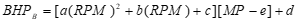
\includegraphics[width=6.5in,height=3.40632in]{media/01/image2.png}

Translational displacements, rates, accelerations, \& forces are positive along the positive body axes directions. In spite of the simplicity of this logic, it is important to recognize that lift and normal load factor are positive in the \emph{negative z} direction and the drag is positive in the \emph{negative x} direction.

Angular displacements, rates, accelerations \& moments, are positive according to the ``right hand rule'' (a clockwise rotation while looking in the direction of the positive axis) as shown in the figure.

The body axes, forces \& translations along them, and moments \& rotations about them are shown with arrows indicating the positive direction.

Angular displacements, rates, accelerations \& moments, are positive according to the ``right hand rule'' (a clockwise rotation while looking in the direction of the positive axis) as shown in the figure.

The body axes, forces \& translations along them, and moments \& rotations about them are shown with arrows indicating the positive direction.

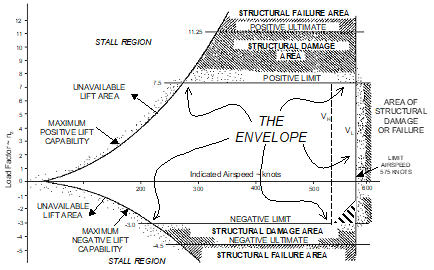
\includegraphics[width=6.5in,height=4.87431in]{media/01/image3.png}

Angle of attack is positive clockwise from the projection of the velocity vector on the \emph{xz} plane to the reference \emph{x} body axis. The angle of sideslip is positive clockwise from the \emph{xz} plane to the velocity vector (wind in the pilot's right ear).

Aircraft \emph{true} heading is the angle between \emph{true} North and the projection of the x-body axis onto the horizontal plane. Mag. heading refers to mag North

The velocity vector is measured relative to the air mass while the flightpath is measured relative to the ground. They are equivalent only when winds are zero.

Flightpath heading angle (ground track heading)~\(\sigma_g\),~is the horizontal angle between true North and the projection of the flightpath on the horizontal plane. Positive rotation is from north to east.

Flightpath elevation angle;~\emph{γ}, is the vertical angle between the flightpath and the horizontal plane. Positive rotation is up. During a descent, this parameter is commonly known as glide path angle.

Flightpath bank angle;~\(\mu\), is the angle between the plane formed by the velocity vector and the lift vector and the vertical plane containing the velocity vector. Positive rotation is clockwise about the velocity vector, looking forward.

Fuselage reference station (FRS), Water line (WL), and Buttock line (BL) are reference coordinates established by the design group.

\begin{longtable}[]{@{}lll@{}}
\toprule
\textbf{Summary of Generally Accepted Body Axes Sign Convention} & &\tabularnewline
\midrule
\endhead
\textbf{Parameter Name} & \textbf{Symbol} & \textbf{Positive Direction}\tabularnewline
Translational Measurements & &\tabularnewline
Longitudinal axis & \(x\) & from ref \emph{cg} towards nose\tabularnewline
Lateral axis & \(y\) & from reference \emph{cg} towards right wing tip\tabularnewline
Vertical axis & \(z\) & from reference \emph{cg} towards vehicle bottom (body axis)\tabularnewline
Longitudinal velocity & \(u\) & along +x axis\tabularnewline
Lateral velocity & \(v\) & along +y axis\tabularnewline
Vertical velocity & \(w\) & along +z axis\tabularnewline
Longitudinal acceleration & \(a_x\) & along +x axis\tabularnewline
Lateral acceleration & \(a_y\) & along +y axis\tabularnewline
Vertical acceleration & \(a_z\) & along +z axis\tabularnewline
Longitudinal load factor & \(N_x\) & along +x axis\tabularnewline
Lateral load factor & \(N_y\) & along +y-axis\tabularnewline
Normal load factor & \(N_z\) & along -z axis\tabularnewline
Longitudinal force & \(F_x\) & along the +x axis\tabularnewline
Lateral force & \(F_y\) & along the +y axis\tabularnewline
Normal force & \(F_z\) & along the + z axis\tabularnewline
Drag force & \(D\) & along the -x axis\tabularnewline
Side force & \(Y\) & along the + y axis\tabularnewline
Lift Force & \(L\) & along the -z axis\tabularnewline
\bottomrule
\end{longtable}

\textbf{Summary of Generally Accepted Body Axes Sign Convention}

\begin{longtable}[]{@{}lcl@{}}
\toprule
\begin{minipage}[b]{0.56\columnwidth}\raggedright
\textbf{Parameter Name}\strut
\end{minipage} & \begin{minipage}[b]{0.12\columnwidth}\centering
\textbf{Symbol}\strut
\end{minipage} & \begin{minipage}[b]{0.23\columnwidth}\raggedright
\textbf{Positive Direction}\strut
\end{minipage}\tabularnewline
\midrule
\endhead
\begin{minipage}[t]{0.56\columnwidth}\raggedright
Angular Measurements\strut
\end{minipage} & \begin{minipage}[t]{0.12\columnwidth}\centering
\strut
\end{minipage} & \begin{minipage}[t]{0.23\columnwidth}\raggedright
\strut
\end{minipage}\tabularnewline
\begin{minipage}[t]{0.56\columnwidth}\raggedright
Bank angle\strut
\end{minipage} & \begin{minipage}[t]{0.12\columnwidth}\centering
\(\phi\)\strut
\end{minipage} & \begin{minipage}[t]{0.23\columnwidth}\raggedright
right wing down\strut
\end{minipage}\tabularnewline
\begin{minipage}[t]{0.56\columnwidth}\raggedright
Pitch angle\strut
\end{minipage} & \begin{minipage}[t]{0.12\columnwidth}\centering
\(\theta\)\strut
\end{minipage} & \begin{minipage}[t]{0.23\columnwidth}\raggedright
nose-up\strut
\end{minipage}\tabularnewline
\begin{minipage}[t]{0.56\columnwidth}\raggedright
Heading\strut
\end{minipage} & \begin{minipage}[t]{0.12\columnwidth}\centering
\(\psi\)\strut
\end{minipage} & \begin{minipage}[t]{0.23\columnwidth}\raggedright
0 North, +Eastward\strut
\end{minipage}\tabularnewline
\begin{minipage}[t]{0.56\columnwidth}\raggedright
Angle of attack\strut
\end{minipage} & \begin{minipage}[t]{0.12\columnwidth}\centering
\(\alpha\)\strut
\end{minipage} & \begin{minipage}[t]{0.23\columnwidth}\raggedright
normal flight attitude\strut
\end{minipage}\tabularnewline
\begin{minipage}[t]{0.56\columnwidth}\raggedright
Angle of sideslip\strut
\end{minipage} & \begin{minipage}[t]{0.12\columnwidth}\centering
\(\beta\)\strut
\end{minipage} & \begin{minipage}[t]{0.23\columnwidth}\raggedright
``wind in the right ear''\strut
\end{minipage}\tabularnewline
\begin{minipage}[t]{0.56\columnwidth}\raggedright
Roll rate\strut
\end{minipage} & \begin{minipage}[t]{0.12\columnwidth}\centering
\(p\)\strut
\end{minipage} & \begin{minipage}[t]{0.23\columnwidth}\raggedright
right wing down\strut
\end{minipage}\tabularnewline
\begin{minipage}[t]{0.56\columnwidth}\raggedright
Pitch rate\strut
\end{minipage} & \begin{minipage}[t]{0.12\columnwidth}\centering
\(q\)\strut
\end{minipage} & \begin{minipage}[t]{0.23\columnwidth}\raggedright
nose up\strut
\end{minipage}\tabularnewline
\begin{minipage}[t]{0.56\columnwidth}\raggedright
Yaw rate\strut
\end{minipage} & \begin{minipage}[t]{0.12\columnwidth}\centering
\(r\)\strut
\end{minipage} & \begin{minipage}[t]{0.23\columnwidth}\raggedright
nose right\strut
\end{minipage}\tabularnewline
\begin{minipage}[t]{0.56\columnwidth}\raggedright
Roll moment\strut
\end{minipage} & \begin{minipage}[t]{0.12\columnwidth}\centering
\(L\)\strut
\end{minipage} & \begin{minipage}[t]{0.23\columnwidth}\raggedright
right wing down\strut
\end{minipage}\tabularnewline
\begin{minipage}[t]{0.56\columnwidth}\raggedright
Pitch moment\strut
\end{minipage} & \begin{minipage}[t]{0.12\columnwidth}\centering
\(M\)\strut
\end{minipage} & \begin{minipage}[t]{0.23\columnwidth}\raggedright
nose up\strut
\end{minipage}\tabularnewline
\begin{minipage}[t]{0.56\columnwidth}\raggedright
Yaw moment\strut
\end{minipage} & \begin{minipage}[t]{0.12\columnwidth}\centering
\(N\)\strut
\end{minipage} & \begin{minipage}[t]{0.23\columnwidth}\raggedright
nose right\strut
\end{minipage}\tabularnewline
\begin{minipage}[t]{0.56\columnwidth}\raggedright
Flightpath bank angle\strut
\end{minipage} & \begin{minipage}[t]{0.12\columnwidth}\centering
\(\mu\)\strut
\end{minipage} & \begin{minipage}[t]{0.23\columnwidth}\raggedright
right wing down\strut
\end{minipage}\tabularnewline
\begin{minipage}[t]{0.56\columnwidth}\raggedright
Flightpath elevation\strut
\end{minipage} & \begin{minipage}[t]{0.12\columnwidth}\centering
\(\gamma\)\strut
\end{minipage} & \begin{minipage}[t]{0.23\columnwidth}\raggedright
climb\strut
\end{minipage}\tabularnewline
\begin{minipage}[t]{0.56\columnwidth}\raggedright
Flightpath heading\strut
\end{minipage} & \begin{minipage}[t]{0.12\columnwidth}\centering
\(\sigma_g\)\strut
\end{minipage} & \begin{minipage}[t]{0.23\columnwidth}\raggedright
0 true North, + East-

ward\strut
\end{minipage}\tabularnewline
\bottomrule
\end{longtable}

Discussion of ``Input \& Deflection'' Conventions

The debate regarding proper inputs and deflections stems from the user's viewpoint. From the body axis convention above, flight testers recognize that a climbing right turn generates positive angular measurements. Logically then, pull, right roll and right yaw pilot inputs and subsequent surface deflections should also be positive. The traditional flight tester's convention follows as ``All input forces \& displacements, surface deflections, and motions that cause a climbing right turn are positive.''

Due to differential nature of aileron deflections, they require more discussion. The flight tester's logic implies (but does not dictate) positive deflections are right aileron up and left aileron down. It is, however, equally acceptable to assign downward (or upward) deflection as positive for \underline{both} ailerons and calculate the difference between the two as a measure of rolling moment.

The rationale within the wind tunnel community is also logical: any control surface deflection that increases lift is positive. From this, positive deflections are trailing edge down (TED) for each: trailing edge flap, stabilizer, elevator, stabilator, rollervator, ruddervator, canard, aileron, flaperon, and all their tabs. Leading edge flap down is also positive. Similarly, since side force is positive to the right, then positive rudder and rudder tab deflections are trailing left (TEL). The only exception to this straightforward logic is for spoilers and speed brakes that extend only in one direction: this deflection is positive even though it might decrease the lift.

Since the above rationale defines downward deflection as positive for both ailerons, a measurement of rolling moments requires calculation of the differential aileron deflection. This rationale does not, however, specifically dictate whether a ``positive'' differential deflection should generate right wing down (RWD) or left wing down (LWD) moments. Differential aileron can be calculated as either.

\(\delta_{a} = \frac{\delta_{\mathrm{a_R}} - \delta_{\mathrm{a_L}}}{2}\) or \(\delta_{a} = \frac{\delta_{\mathrm{a_L}} - \delta_{\mathrm{a_R}}}{2}\)

Selection of the RWD convention is obvious from the flight tester's viewpoint since deflections that generate right rolls are positive. An alternative interpretation is that a positive differential aileron deflection is one that lifts the positive (right) wing lifts more than the left (LWD).

Another common convention for ailerons is one that gives the same sign to both ailerons for any input. The ``right hand screw'' convention is opposite to the flight tester's convention, but may be more common:

\(\delta_{a_R} = +\mathrm{TED}\), \(\delta_{a_L} = +\mathrm{TEU}\).

The above wind tunnel rationale dictates only the polarity for individual control surface deflections, and leaves open the sign convention debate about controller (inceptor) input forces \& displacements. One approach is that positive inputs should generate positive \emph{motions} while an alternate approach is that positive inputs generate positive \emph{surface deflections}. Only the flight tester's convention states that positive inputs yield positive motions \emph{and} deflections. All approaches are mathematically connected to the hinge moment sign convention discussed below.

The simplest control surface hinge moment convention is that \emph{all} positive hinge moments (generated by the pilot and the aerodynamics) move the surface in a positive direction, i.e., positive input forces yield positive deflections. This has different implications for the different sign conventions:

•~According to the above flight tester's sign convention, a positive pull force is required to generate a positive (TEU) elevator deflection (positive stick force generates a climb).

•~According to wind tunnel sign convention, a positive \emph{push} force is required to generate a positive (\emph{TED}) elevator deflection (positive stick force generates a \emph{dive}).

The alternate viewpoint defines a positive inceptor hinge moment as one that \emph{opposes} the aerodynamic moments. In other words, a positive inceptor hinge moment moves the surface to a position which generates positive aerodynamic hinge moments or ``positive input forces \& displacements generate negative surface deflections.''

Based on the above background, the SFTE technical council proposes the following standard convention for inceptor \& surface forces \& deflections:

•~Due to its widespread use and its simple \& robust nature, use the wind tunnel convention for control surface deflections.

•~Due to widespread test pilot \& FTE familiarity and logical nature, use the flight tester's convention that positive inceptor forces \& displacements generate a climbing right turn.

•~A fallout from these conventions is that positive inceptor hinge moments generate positive aerodynamic hinge moments (negative surface deflections).

•~Consistent use of the above logic requires that the calculated value for aileron deflection be negative for right wing down moments. Similarly, differential ruddervator deflections generating nose right yawing moments should have negative values.

\textbf{~}

\textbf{Conventions for Positive Control Surface Deflections}

\begin{longtable}[]{@{}lccc@{}}
\toprule
\begin{minipage}[b]{0.19\columnwidth}\raggedright
\textbf{Parameter}\strut
\end{minipage} & \begin{minipage}[b]{0.14\columnwidth}\centering
\textbf{Symbol}\strut
\end{minipage} & \begin{minipage}[b]{0.29\columnwidth}\centering
\textbf{Flight Test}\strut
\end{minipage} & \begin{minipage}[b]{0.27\columnwidth}\centering
\textbf{SFTE/}
\textbf{Wind Tunnel}\strut
\end{minipage}\tabularnewline
\midrule
\endhead
\begin{minipage}[t]{0.19\columnwidth}\raggedright
Horizontal Stabilizer\strut
\end{minipage} & \begin{minipage}[t]{0.14\columnwidth}\centering
\(\delta_i\)\strut
\end{minipage} & \begin{minipage}[t]{0.29\columnwidth}\centering
TEU\strut
\end{minipage} & \begin{minipage}[t]{0.27\columnwidth}\centering
TED\strut
\end{minipage}\tabularnewline
\begin{minipage}[t]{0.19\columnwidth}\raggedright
Elevator\strut
\end{minipage} & \begin{minipage}[t]{0.14\columnwidth}\centering
\(\delta_e\)\strut
\end{minipage} & \begin{minipage}[t]{0.29\columnwidth}\centering
TEU\strut
\end{minipage} & \begin{minipage}[t]{0.27\columnwidth}\centering
TED\strut
\end{minipage}\tabularnewline
\begin{minipage}[t]{0.19\columnwidth}\raggedright
Elev. Tab\strut
\end{minipage} & \begin{minipage}[t]{0.14\columnwidth}\centering
\(\delta_{et}\)\strut
\end{minipage} & \begin{minipage}[t]{0.29\columnwidth}\centering
TED\strut
\end{minipage} & \begin{minipage}[t]{0.27\columnwidth}\centering
TED\strut
\end{minipage}\tabularnewline
\begin{minipage}[t]{0.19\columnwidth}\raggedright
Stabilators or Rollervators,\strut
\end{minipage} & \begin{minipage}[t]{0.14\columnwidth}\centering
\(\delta_{eL}\),
\(\delta_{eR}\)\strut
\end{minipage} & \begin{minipage}[t]{0.29\columnwidth}\centering
TEU\strut
\end{minipage} & \begin{minipage}[t]{0.27\columnwidth}\centering
TED\strut
\end{minipage}\tabularnewline
\begin{minipage}[t]{0.19\columnwidth}\raggedright
average:\strut
\end{minipage} & \begin{minipage}[t]{0.14\columnwidth}\centering
\(\delta_e\)\strut
\end{minipage} & \begin{minipage}[t]{0.29\columnwidth}\centering
\[\frac{\delta_{eR} + \delta_{eL}}{2}\]\strut
\end{minipage} & \begin{minipage}[t]{0.27\columnwidth}\centering
\strut
\end{minipage}\tabularnewline
\begin{minipage}[t]{0.19\columnwidth}\raggedright
differential:\strut
\end{minipage} & \begin{minipage}[t]{0.14\columnwidth}\centering
\(\Delta\delta_e\)\strut
\end{minipage} & \begin{minipage}[t]{0.29\columnwidth}\centering
\[\frac{\delta_{eR} - \delta_{eL}}{2}\]\strut
\end{minipage} & \begin{minipage}[t]{0.27\columnwidth}\centering
\strut
\end{minipage}\tabularnewline
\begin{minipage}[t]{0.19\columnwidth}\raggedright
Elevons\strut
\end{minipage} & \begin{minipage}[t]{0.14\columnwidth}\centering
\(\delta_{vL}\),
\(\delta_{vR}\)\strut
\end{minipage} & \begin{minipage}[t]{0.29\columnwidth}\centering
TEU\strut
\end{minipage} & \begin{minipage}[t]{0.27\columnwidth}\centering
TED\strut
\end{minipage}\tabularnewline
\begin{minipage}[t]{0.19\columnwidth}\raggedright
average:\strut
\end{minipage} & \begin{minipage}[t]{0.14\columnwidth}\centering
\(\delta_v\)\strut
\end{minipage} & \begin{minipage}[t]{0.29\columnwidth}\centering
\[\frac{\delta_{vR} + \delta_{vL}}{2}\]\strut
\end{minipage} & \begin{minipage}[t]{0.27\columnwidth}\centering
\strut
\end{minipage}\tabularnewline
\begin{minipage}[t]{0.19\columnwidth}\raggedright
differential:\strut
\end{minipage} & \begin{minipage}[t]{0.14\columnwidth}\centering
\(\Delta\delta_v\)\strut
\end{minipage} & \begin{minipage}[t]{0.29\columnwidth}\centering
\[\frac{\delta_{vR} - \delta_{vL}}{2}\]\strut
\end{minipage} & \begin{minipage}[t]{0.27\columnwidth}\centering
\strut
\end{minipage}\tabularnewline
\begin{minipage}[t]{0.19\columnwidth}\raggedright
Flaperons or trailing edge flap\strut
\end{minipage} & \begin{minipage}[t]{0.14\columnwidth}\centering
\(\delta_{fL}\),
\(\delta_{fR}\)\strut
\end{minipage} & \begin{minipage}[t]{0.29\columnwidth}\centering
TED\strut
\end{minipage} & \begin{minipage}[t]{0.27\columnwidth}\centering
TED\strut
\end{minipage}\tabularnewline
\begin{minipage}[t]{0.19\columnwidth}\raggedright
average:\strut
\end{minipage} & \begin{minipage}[t]{0.14\columnwidth}\centering
\(\delta_f\)\strut
\end{minipage} & \begin{minipage}[t]{0.29\columnwidth}\centering
\[\frac{\delta_{fR} + \delta_{fL}}{2}\]\strut
\end{minipage} & \begin{minipage}[t]{0.27\columnwidth}\centering
\strut
\end{minipage}\tabularnewline
\begin{minipage}[t]{0.19\columnwidth}\raggedright
differential:\strut
\end{minipage} & \begin{minipage}[t]{0.14\columnwidth}\centering
\(\Delta\delta_f\)\strut
\end{minipage} & \begin{minipage}[t]{0.29\columnwidth}\centering
\[-\frac{\delta_{fR} - \delta_{fL}}{2}\]\strut
\end{minipage} & \begin{minipage}[t]{0.27\columnwidth}\centering
\[\frac{\delta_{fR} - \delta_{fL}}{2}\]\strut
\end{minipage}\tabularnewline
\begin{minipage}[t]{0.19\columnwidth}\raggedright
Canards\strut
\end{minipage} & \begin{minipage}[t]{0.14\columnwidth}\centering
\(\delta_{cL}\),
\(\delta_{cR}\)\strut
\end{minipage} & \begin{minipage}[t]{0.29\columnwidth}\centering
TED\strut
\end{minipage} & \begin{minipage}[t]{0.27\columnwidth}\centering
TED\strut
\end{minipage}\tabularnewline
\begin{minipage}[t]{0.19\columnwidth}\raggedright
average:\strut
\end{minipage} & \begin{minipage}[t]{0.14\columnwidth}\centering
\(\delta_c\)\strut
\end{minipage} & \begin{minipage}[t]{0.29\columnwidth}\centering
\[\frac{\delta_{cR} + \delta_{cL}}{2}\]\strut
\end{minipage} & \begin{minipage}[t]{0.27\columnwidth}\centering
\strut
\end{minipage}\tabularnewline
\begin{minipage}[t]{0.19\columnwidth}\raggedright
differential:\strut
\end{minipage} & \begin{minipage}[t]{0.14\columnwidth}\centering
\(\Delta\delta_c\)\strut
\end{minipage} & \begin{minipage}[t]{0.29\columnwidth}\centering
\[-\frac{\delta_{cR} - \delta_{cL}}{2}\]\strut
\end{minipage} & \begin{minipage}[t]{0.27\columnwidth}\centering
\[\frac{\delta_{cR} - \delta_{cL}}{2}\]\strut
\end{minipage}\tabularnewline
\begin{minipage}[t]{0.19\columnwidth}\raggedright
Leading edge flap\strut
\end{minipage} & \begin{minipage}[t]{0.14\columnwidth}\centering
\(\delta_{lefL}\),
\(\delta_{lefR}\)\strut
\end{minipage} & \begin{minipage}[t]{0.29\columnwidth}\centering
Leading Edge Down\strut
\end{minipage} & \begin{minipage}[t]{0.27\columnwidth}\centering
Leading Edge Down\strut
\end{minipage}\tabularnewline
\begin{minipage}[t]{0.19\columnwidth}\raggedright
Ruddervators\strut
\end{minipage} & \begin{minipage}[t]{0.14\columnwidth}\centering
\(\delta_{rvL}\),
\(\delta_{rvR}\)\strut
\end{minipage} & \begin{minipage}[t]{0.29\columnwidth}\centering
TEU\strut
\end{minipage} & \begin{minipage}[t]{0.27\columnwidth}\centering
TED\strut
\end{minipage}\tabularnewline
\begin{minipage}[t]{0.19\columnwidth}\raggedright
average:\strut
\end{minipage} & \begin{minipage}[t]{0.14\columnwidth}\centering
\(\delta_{rv}\)\strut
\end{minipage} & \begin{minipage}[t]{0.29\columnwidth}\centering
\[\frac{\delta_{rvR}+\delta_{rvL}}{2}\]\strut
\end{minipage} & \begin{minipage}[t]{0.27\columnwidth}\centering
\strut
\end{minipage}\tabularnewline
\begin{minipage}[t]{0.19\columnwidth}\raggedright
differential:\strut
\end{minipage} & \begin{minipage}[t]{0.14\columnwidth}\centering
\(\Delta\delta_{rv}\)\strut
\end{minipage} & \begin{minipage}[t]{0.29\columnwidth}\centering
\[-\frac{\delta_{rvR} - \delta_{rvL}}{2}\]\strut
\end{minipage} & \begin{minipage}[t]{0.27\columnwidth}\centering
\strut
\end{minipage}\tabularnewline
\begin{minipage}[t]{0.19\columnwidth}\raggedright
Ailerons\strut
\end{minipage} & \begin{minipage}[t]{0.14\columnwidth}\centering
\(\delta_{aL}\),
\(\delta_{aR}\)\strut
\end{minipage} & \begin{minipage}[t]{0.29\columnwidth}\centering
\(\delta_{aR}\) TEU \&~\(\delta_{aL}\) TED

or

\(\delta_{aR}\) \& \(\delta_{aL}\) TED\strut
\end{minipage} & \begin{minipage}[t]{0.27\columnwidth}\centering
\(\delta_{aR}\) \& \(\delta_{aL}\) TED\strut
\end{minipage}\tabularnewline
\begin{minipage}[t]{0.19\columnwidth}\raggedright
Aileron Tab\strut
\end{minipage} & \begin{minipage}[t]{0.14\columnwidth}\centering
\(\delta_{at}\)\strut
\end{minipage} & \begin{minipage}[t]{0.29\columnwidth}\centering
\[\frac{\delta_{aR}+\delta_{aL}}{2}\]\strut
\end{minipage} & \begin{minipage}[t]{0.27\columnwidth}\centering
\(\delta_{at}\) TED\strut
\end{minipage}\tabularnewline
\begin{minipage}[t]{0.19\columnwidth}\raggedright
average:\strut
\end{minipage} & \begin{minipage}[t]{0.14\columnwidth}\centering
\(\delta_{a}\)\strut
\end{minipage} & \begin{minipage}[t]{0.29\columnwidth}\centering
\[-\frac{\delta_{aR} - \delta_{aL}}{2}\]\strut
\end{minipage} & \begin{minipage}[t]{0.27\columnwidth}\centering
\[\frac{\delta_{aR} - \delta_{aL}}{2}\]\strut
\end{minipage}\tabularnewline
\begin{minipage}[t]{0.19\columnwidth}\raggedright
Spoilers\strut
\end{minipage} & \begin{minipage}[t]{0.14\columnwidth}\centering
\(\delta_{sL}\),
\(\delta_{sR}\)\strut
\end{minipage} & \begin{minipage}[t]{0.29\columnwidth}\centering
Extended\strut
\end{minipage} & \begin{minipage}[t]{0.27\columnwidth}\centering
Extended\strut
\end{minipage}\tabularnewline
\begin{minipage}[t]{0.19\columnwidth}\raggedright
average:\strut
\end{minipage} & \begin{minipage}[t]{0.14\columnwidth}\centering
\(\delta_{s}\)\strut
\end{minipage} & \begin{minipage}[t]{0.29\columnwidth}\centering
\[\frac{\delta_{sR}+\delta_{sL}}{2}\]\strut
\end{minipage} & \begin{minipage}[t]{0.27\columnwidth}\centering
\strut
\end{minipage}\tabularnewline
\begin{minipage}[t]{0.19\columnwidth}\raggedright
differential:\strut
\end{minipage} & \begin{minipage}[t]{0.14\columnwidth}\centering
\(\Delta\delta_{s}\)\strut
\end{minipage} & \begin{minipage}[t]{0.29\columnwidth}\centering
\[\frac{\delta_{sR} - \delta_{sL}}{2}\]\strut
\end{minipage} & \begin{minipage}[t]{0.27\columnwidth}\centering
\[-\frac{\delta_{sR} - \delta_{sL}}{2}\]\strut
\end{minipage}\tabularnewline
\begin{minipage}[t]{0.19\columnwidth}\raggedright
Rudders\strut
\end{minipage} & \begin{minipage}[t]{0.14\columnwidth}\centering
\(\delta_{rL}\),
\(\delta_{rR}\)\strut
\end{minipage} & \begin{minipage}[t]{0.29\columnwidth}\centering
TER\strut
\end{minipage} & \begin{minipage}[t]{0.27\columnwidth}\centering
TEL\strut
\end{minipage}\tabularnewline
\begin{minipage}[t]{0.19\columnwidth}\raggedright
average:\strut
\end{minipage} & \begin{minipage}[t]{0.14\columnwidth}\centering
\(\delta_{r}\)\strut
\end{minipage} & \begin{minipage}[t]{0.29\columnwidth}\centering
\[\frac{\delta_{rR}+\delta_{rL}}{2}\]\strut
\end{minipage} & \begin{minipage}[t]{0.27\columnwidth}\centering
\strut
\end{minipage}\tabularnewline
\begin{minipage}[t]{0.19\columnwidth}\raggedright
Rudder tab\strut
\end{minipage} & \begin{minipage}[t]{0.14\columnwidth}\centering
\(\delta_{rt}\)\strut
\end{minipage} & \begin{minipage}[t]{0.29\columnwidth}\centering
TEL\strut
\end{minipage} & \begin{minipage}[t]{0.27\columnwidth}\centering
\strut
\end{minipage}\tabularnewline
\begin{minipage}[t]{0.19\columnwidth}\raggedright
Speed brake\strut
\end{minipage} & \begin{minipage}[t]{0.14\columnwidth}\centering
\(\delta_{sb}\)\strut
\end{minipage} & \begin{minipage}[t]{0.29\columnwidth}\centering
Extended\strut
\end{minipage} & \begin{minipage}[t]{0.27\columnwidth}\centering
\strut
\end{minipage}\tabularnewline
\bottomrule
\end{longtable}

\textbf{Conventions for Positive Inputs and Hinge Moments}

\begin{longtable}[]{@{}lccc@{}}
\toprule
\begin{minipage}[b]{0.38\columnwidth}\raggedright
\textbf{Parameter}\strut
\end{minipage} & \begin{minipage}[b]{0.20\columnwidth}\centering
\textbf{Symbol}\strut
\end{minipage} & \begin{minipage}[b]{0.15\columnwidth}\centering
\textbf{Flight Test}\strut
\end{minipage} & \begin{minipage}[b]{0.15\columnwidth}\centering
\textbf{SFTE/}
\textbf{Wind Tunnel}\strut
\end{minipage}\tabularnewline
\midrule
\endhead
\begin{minipage}[t]{0.38\columnwidth}\raggedright
Stick/Wheel

Long Force\strut
\end{minipage} & \begin{minipage}[t]{0.20\columnwidth}\centering
\(F_e\)\strut
\end{minipage} & \begin{minipage}[t]{0.15\columnwidth}\centering
Pull\strut
\end{minipage} & \begin{minipage}[t]{0.15\columnwidth}\centering
\strut
\end{minipage}\tabularnewline
\begin{minipage}[t]{0.38\columnwidth}\raggedright
Stick/Wheel

Lateral Force\strut
\end{minipage} & \begin{minipage}[t]{0.20\columnwidth}\centering
\(F_a\)\strut
\end{minipage} & \begin{minipage}[t]{0.15\columnwidth}\centering
Right\strut
\end{minipage} & \begin{minipage}[t]{0.15\columnwidth}\centering
\strut
\end{minipage}\tabularnewline
\begin{minipage}[t]{0.38\columnwidth}\raggedright
Pedal Force\strut
\end{minipage} & \begin{minipage}[t]{0.20\columnwidth}\centering
\(F_r\)\strut
\end{minipage} & \begin{minipage}[t]{0.15\columnwidth}\centering
Right pedal push\strut
\end{minipage} & \begin{minipage}[t]{0.15\columnwidth}\centering
\strut
\end{minipage}\tabularnewline
\begin{minipage}[t]{0.38\columnwidth}\raggedright
Stick/Wheel

Longitudinal deflection\strut
\end{minipage} & \begin{minipage}[t]{0.20\columnwidth}\centering
\(\delta_{s_e}\)\strut
\end{minipage} & \begin{minipage}[t]{0.15\columnwidth}\centering
Aft\strut
\end{minipage} & \begin{minipage}[t]{0.15\columnwidth}\centering
\strut
\end{minipage}\tabularnewline
\begin{minipage}[t]{0.38\columnwidth}\raggedright
Stick/wheel

Lateral deflection\strut
\end{minipage} & \begin{minipage}[t]{0.20\columnwidth}\centering
\(\delta_{s_a}\)\strut
\end{minipage} & \begin{minipage}[t]{0.15\columnwidth}\centering
Right\strut
\end{minipage} & \begin{minipage}[t]{0.15\columnwidth}\centering
\strut
\end{minipage}\tabularnewline
\begin{minipage}[t]{0.38\columnwidth}\raggedright
Pedal deflection\strut
\end{minipage} & \begin{minipage}[t]{0.20\columnwidth}\centering
\(\delta_{pR}\),
\(\delta_{pL}\)\strut
\end{minipage} & \begin{minipage}[t]{0.15\columnwidth}\centering
Right pedal push\strut
\end{minipage} & \begin{minipage}[t]{0.15\columnwidth}\centering
\strut
\end{minipage}\tabularnewline
\begin{minipage}[t]{0.38\columnwidth}\raggedright
Aerodynamic Hinge Moments\strut
\end{minipage} & \begin{minipage}[t]{0.20\columnwidth}\centering
\(C_{h_\delta}\)

\(C_{h_\alpha}\)

\(C_{h_{\delta_o}}\)

\(C_{h_{\delta_\text{tab}}}\)\strut
\end{minipage} & \begin{minipage}[t]{0.15\columnwidth}\centering
positive moments

generate

positive deflections\strut
\end{minipage} & \begin{minipage}[t]{0.15\columnwidth}\centering
\strut
\end{minipage}\tabularnewline
\begin{minipage}[t]{0.38\columnwidth}\raggedright
Inceptor

Hinge Moments\strut
\end{minipage} & \begin{minipage}[t]{0.20\columnwidth}\centering
\(C_{h_{F_e}}\)

\(C_{h_{F_a}}\)

\(C_{h_{F_r}}\)\strut
\end{minipage} & \begin{minipage}[t]{0.15\columnwidth}\centering
+ moments generate

+ deflections\strut
\end{minipage} & \begin{minipage}[t]{0.15\columnwidth}\centering
+ moments generate

- deflections\strut
\end{minipage}\tabularnewline
\bottomrule
\end{longtable}

*The wind tunnel rationale does not inherently define the polarity for control surface differential deflections.

\#The wind tunnel rationale does not specify a convention for positive inputs or hinge moments. Historically, Dutch, U.S. and some British aircraft use a climbing right turn, while it is a diving left turn for Canadian, Australian, and some British aircraft.

\emph{The SFTE Technical Council recognizes that several combinations of the above possibilities are currently in use around the world, and invites comments, additions, or corrections to the above summary and proposal. Although SFTE does not expect all organizations to adopt this standard, it still \textbf{provides a cornerstone for reference purposes}}

\hypertarget{thermodynamics-relations}{%
\section{Thermodynamics Relations}\label{thermodynamics-relations}}

(references 1.3, 1.4, 1.5, 1.6)

\hypertarget{thermodynamic-definitions}{%
\subsection{Thermodynamic Definitions}\label{thermodynamic-definitions}}

A \textbf{Process} is an event with a redistribution of energy within a system.

A \textbf{Reversible} process is one that can be reversed such that the system returns to its original state (form, location \& amount).

An \textbf{Irreversible} process cannot return to its original state due to heat flow from higher to lower temperatures, fluid turbulence, friction, or inelastic deformation. The change in entropy is non-zero.

An \textbf{Isothermal} process is one in which the temperature of the fluid is constant.

An \textbf{Adiabatic} process is one in which heat is not transferred to or from the fluid.

\textbf{Work} is the energy \emph{transfer} by way of changing mechanical energy.

\textbf{Heat} is the energy \emph{transfer} from one body to another by virtue of a temperature difference between them.

An \textbf{Isentropic} process has constant entropy.

\textbf{Conduction} is the energy transfer from a warmer body by tangible contact (transfer of some internal molecular kinetic energy).

\textbf{Convection} is the repositioning the energy of a fluid without state changes or energy transformations (e.g.~heated air moving from one room to another room).

\textbf{Radiation} is the energy transmission through space.

\hypertarget{thermodynamic-symbols}{%
\subsection{Thermodynamic Symbols}\label{thermodynamic-symbols}}

\begin{longtable}[]{@{}ll@{}}
\toprule
\begin{minipage}[b]{0.58\columnwidth}\raggedright
Symbol\strut
\end{minipage} & \begin{minipage}[b]{0.36\columnwidth}\raggedright
Use\strut
\end{minipage}\tabularnewline
\midrule
\endhead
\begin{minipage}[t]{0.58\columnwidth}\raggedright
\(A\)\strut
\end{minipage} & \begin{minipage}[t]{0.36\columnwidth}\raggedright
area\strut
\end{minipage}\tabularnewline
\begin{minipage}[t]{0.58\columnwidth}\raggedright
\(C\)\strut
\end{minipage} & \begin{minipage}[t]{0.36\columnwidth}\raggedright
compressibility factor\strut
\end{minipage}\tabularnewline
\begin{minipage}[t]{0.58\columnwidth}\raggedright
\(c\)\strut
\end{minipage} & \begin{minipage}[t]{0.36\columnwidth}\raggedright
speed of sound\strut
\end{minipage}\tabularnewline
\begin{minipage}[t]{0.58\columnwidth}\raggedright
\(E = u\)\strut
\end{minipage} & \begin{minipage}[t]{0.36\columnwidth}\raggedright
specific internal energy (e.g.~Btu/lb)\strut
\end{minipage}\tabularnewline
\begin{minipage}[t]{0.58\columnwidth}\raggedright
\(H\)\strut
\end{minipage} & \begin{minipage}[t]{0.36\columnwidth}\raggedright
specific \textbf{enthalpy} (e.g.~Btu/lb)\strut
\end{minipage}\tabularnewline
\begin{minipage}[t]{0.58\columnwidth}\raggedright
\(J\)\strut
\end{minipage} & \begin{minipage}[t]{0.36\columnwidth}\raggedright
Joule\strut
\end{minipage}\tabularnewline
\begin{minipage}[t]{0.58\columnwidth}\raggedright
\(Q\)\strut
\end{minipage} & \begin{minipage}[t]{0.36\columnwidth}\raggedright
energy supplied to a system or region as heat (e.g.~Btu/lb)\strut
\end{minipage}\tabularnewline
\begin{minipage}[t]{0.58\columnwidth}\raggedright
\(P\)\strut
\end{minipage} & \begin{minipage}[t]{0.36\columnwidth}\raggedright
absolute pressure (e.g.~lbs/ft\textsuperscript{2})\strut
\end{minipage}\tabularnewline
\begin{minipage}[t]{0.58\columnwidth}\raggedright
\(V\)\strut
\end{minipage} & \begin{minipage}[t]{0.36\columnwidth}\raggedright
specific volume (e.g.~ft\textsuperscript{3}/lb)\strut
\end{minipage}\tabularnewline
\begin{minipage}[t]{0.58\columnwidth}\raggedright
\(W\)\strut
\end{minipage} & \begin{minipage}[t]{0.36\columnwidth}\raggedright
work (+ if entering)\strut
\end{minipage}\tabularnewline
\begin{minipage}[t]{0.58\columnwidth}\raggedright
\(\overline{V}\)\strut
\end{minipage} & \begin{minipage}[t]{0.36\columnwidth}\raggedright
velocity\strut
\end{minipage}\tabularnewline
\begin{minipage}[t]{0.58\columnwidth}\raggedright
\(\Delta\)\strut
\end{minipage} & \begin{minipage}[t]{0.36\columnwidth}\raggedright
change ( final - initial value)\strut
\end{minipage}\tabularnewline
\begin{minipage}[t]{0.58\columnwidth}\raggedright
\(Z\)\strut
\end{minipage} & \begin{minipage}[t]{0.36\columnwidth}\raggedright
altitude\strut
\end{minipage}\tabularnewline
\begin{minipage}[t]{0.58\columnwidth}\raggedright
\(S\)\strut
\end{minipage} & \begin{minipage}[t]{0.36\columnwidth}\raggedright
specific entropy\strut
\end{minipage}\tabularnewline
\begin{minipage}[t]{0.58\columnwidth}\raggedright
\(R\)\strut
\end{minipage} & \begin{minipage}[t]{0.36\columnwidth}\raggedright
gas constant for each gas (for air = 287 J/kg/K = 53.35 ft-lb/lb\textsubscript{m}R)\strut
\end{minipage}\tabularnewline
\begin{minipage}[t]{0.58\columnwidth}\raggedright
\(\overline{R}\)\strut
\end{minipage} & \begin{minipage}[t]{0.36\columnwidth}\raggedright
universal gas constant = 8.314 kJ/kmol/K = 1545 ft lb/lbmol/R\strut
\end{minipage}\tabularnewline
\begin{minipage}[t]{0.58\columnwidth}\raggedright
\(M\)\strut
\end{minipage} & \begin{minipage}[t]{0.36\columnwidth}\raggedright
molar mass (for air = 28.97 kg/kmol)\strut
\end{minipage}\tabularnewline
\begin{minipage}[t]{0.58\columnwidth}\raggedright
\(N\)\strut
\end{minipage} & \begin{minipage}[t]{0.36\columnwidth}\raggedright
number of moles\strut
\end{minipage}\tabularnewline
\begin{minipage}[t]{0.58\columnwidth}\raggedright
\(\rho\)\strut
\end{minipage} & \begin{minipage}[t]{0.36\columnwidth}\raggedright
density\strut
\end{minipage}\tabularnewline
\bottomrule
\end{longtable}

\hypertarget{thermodynamic-laws}{%
\subsection{Thermodynamic Laws}\label{thermodynamic-laws}}

The \textbf{First Law of Thermodynamics} shows that the net amount of energy added to a system equals the net change in energy within the system (Principle of Conservation of Energy): \(W + Q = (E_2 - E_1)\)

The \textbf{Second Law of Thermodynamics} states that entropy increases during any irreversible process: \(S_2 > S_1\)

\textbf{Ideal Gas Equation of State} (a.k.a. Perfect gas law):

\begin{align}
PV&=RT\\
P &= \rho RT\\
PV &= mRT\\
PV &= nRT\\
\end{align}

\[\delta = \sigma \theta\]

where

\begin{align}
\delta &= \frac{P_a}{P_0}\\
\sigma &= \frac{\rho_a}{\rho_0}\\
\theta &= \frac{T_a}{T_0}
\end{align}

\textbf{Boyle's Law} states that when the temperature of a given mass of gas is held constant, then the volume and pressure vary inversely.

\[P_1 V_1 = P_2 V_2\]

where \[T_1 = T_2\]

\textbf{Charles' Law} states that when a volume of a given mass is held constant, then the change in pressure of the gas is proportional to the change in temperature.

\[\frac{P_1}{T_1} = \frac{P_2}{T_2}\]

where \[V_1 = V_2\]

\textbf{Real Gas} Relation:

\[PV = CRT\]

For reversible processes:

\begin{align}
W &= −\int_{}^{}{PdV}\\
Q &= \int_{}^{}{TdS}
\end{align}

For reversible adiabatic processes:

\begin{align}
\frac{P_1}{P_2} &= \Bigg[ \frac{V_2}{V_1} \Bigg]^{\gamma} \\
\frac{T_1}{T_2} &= \Bigg[ \frac{V_2}{V_1} \Bigg]^{\gamma - 1} \\
\frac{T_1}{T_2} &= \Bigg[ \frac{P_1}{P_2} \Bigg]^{\frac{\gamma - 1}{\gamma}} \\
\frac{P_1}{P_2} &= \Bigg[ \frac{\rho_1}{\rho_2} \Bigg]^{\gamma} \\
\end{align}

Steady Flow Energy Equation

\[
Q + H_1 + \frac{\overline{V}_1^2}{2g} + Z_1 = W + H_2 + \frac{\overline{V}_2^2}{2g} + Z_2
\]~

Bernoulli Equation:

\[
\frac{\Delta P}{\rho g} + \frac{\overline{V}_2^2 - \overline{V}_1^2}{2g} + \Delta Z = 0
\]

Flow per Unit Area:

\[
\frac{W}{A} = \sqrt{\frac{\gamma}{R} \frac{P}{\sqrt{T}} \frac{M}{
  \Big( 1 + \frac{\gamma - 1}{2} M^2 \Big) \frac{\gamma + 1}{2 (\gamma - 1)}
}}
\]

Velocity of sound in a perfect gas:

\[
c = \sqrt{\gamma g R T}
\]

Development of \textbf{Specific Heat Relations}:

Specific heat at constant pressure (for air = 1004.76 J/kg/K)
\[
c_p \equiv \frac{\partial H}{\partial T} \Bigg\rvert_{P}
\]

Specific heat at constant volume (for air = 717.986 J/kg/K)
\[
c_v \equiv \frac{\partial u}{\partial T} \Bigg\rvert_{V}
\]

Ratio of specific heats
\[
\kappa = \gamma \equiv \frac{c_p}{c_v}
\]

Enthalpy equation in differential form is: \[dH = du + d(PV)\]

Substituting definitions and ideal gas law gives

\begin{align}
c_p \, dT &= c_v \, dT + R \, dt\\
&\;\;\mathrm{or} \\
c_p &= c_v + R
\end{align}

Rearranging gives

\begin{align}
c_p &= R \frac{\kappa}{\kappa - 1}\\
&\;\;\mathrm{and} \\
c_v &= R \frac{1}{\kappa - 1}
\end{align}

Development of \textbf{Poisson's Equation}:

1)~From the 1st law: \[W+Q = E_2-E_1\]

2)~Substitution for each term gives: \[T\,dS - P\,dV = du\]

3)~Divide through by T: \[dS = \frac{du}{T} + \frac{P\,dV}{T}\]

4)~Recall: \[du = c_v\,dT\] and \[PV = RT\]

5)~Substitution gives: \[dS = c_v\frac{dT}{T} + R \frac{dV}{V}\]

6)~Assume constant specific heat and integrate: \[s_2 - s_1 = c_v\,\ln \frac{T_2}{T_1} + R\,\ln \frac{V_2}{V_1}\]

7)~Assuming a reversible adiabatic process: \[c_v\,\ln \frac{T_2}{T_1} = - R\,\ln \frac{V_2}{V_1}\]

8)~Substitute \[c_v = R\frac{1}{\kappa - 1}\] to get: \[\frac{T_2}{T_1} = \Big( \frac{V_1}{V_2} \Big)^{\kappa -1}\]

9)~Differentiate H: \[dH = du + P\,dV + V\,dP\]

10)~Substitution into step \#2: \[T\,dS = dH - V\,dP\]

11)~Integrate: \[s_2 - s_1 = c_p\,\ln \frac{T_2}{T_1} + R\,\ln \frac{P_2}{P_1}\]

12)~Assuming a reversible adiabatic process: \[c_p\,\ln \frac{T_2}{T_1} = - R\,\ln \frac{P_2}{P_1}\]

13)~Substitute \[c_v = R\frac{\kappa}{\kappa - 1}\] to get: \[\frac{T_2}{T_1} = \Big( \frac{P_2}{P_1} \Big)^{\frac{\kappa -1}{\kappa}}\]

14)~Combine steps \#8, \#13 to get: \[\frac{P_2}{P_1}=\Big( \frac{V_1}{V_2} \Big)^{\kappa}\] or \[(PV)^{\kappa} = \mathrm{const}\]

\hypertarget{mechanics-relations}{%
\section{Mechanics Relations}\label{mechanics-relations}}

\hypertarget{mechanics-symbols}{%
\subsection{Mechanics Symbols}\label{mechanics-symbols}}

\begin{longtable}[]{@{}ll@{}}
\toprule
Symbol & Use\tabularnewline
\midrule
\endhead
\(a\) & linear acceleration\tabularnewline
\(a_r\) & centripetal (radial) acceleration\tabularnewline
\(a_T\) & tangential acceleration\tabularnewline
\(F\) & force\tabularnewline
\(g\) & acceleration due to gravity\tabularnewline
\(G\) & moment\tabularnewline
\(H\) & angular momentum\tabularnewline
\(H\) & height\tabularnewline
\(Hp\) & horsepower\tabularnewline
\(I\) & rotational moment of inertia (see section 10)\tabularnewline
\(J\) & impulse = change in momentum\tabularnewline
\(k\) & radius of gyration\tabularnewline
\(m\) & mass\tabularnewline
\(N_r\) & radial load factor\tabularnewline
\(P\) & power\tabularnewline
\(L\) & linear momentum\tabularnewline
\(Q\) & moment (a.k.a. torque)\tabularnewline
\(r\) & radius\tabularnewline
\(S\) & distance, displacement\tabularnewline
\(s\) & seconds\tabularnewline
\(t\) & time\tabularnewline
\(V\) & true inertial velocity\tabularnewline
\(V_0\) & initial inertial velocity\tabularnewline
\(W\) & work\tabularnewline
\(q\) & angular displacement\tabularnewline
\(\mathrm{Vol}\) & volume\tabularnewline
\(\omega\) & angular velocity (radians/second)\tabularnewline
\(\dot{\omega}\) & angular acceleration\tabularnewline
\bottomrule
\end{longtable}

\hypertarget{newtons-laws}{%
\subsection{Newton's Laws}\label{newtons-laws}}

\textbf{1\textsuperscript{st} law} (law of inertia):

``Every body persists in its state of rest or uniform motion in a straight line unless it is compelled to change that state by forces impressed on it.''

\textbf{2\textsuperscript{nd} Law}:

``The change in motion is proportional to the motive force impressed and is made in the direction of the straight line in which that force is impressed'' (motion defined as velocity \emph{x} quantity of matter or linear momentum, \(m\,V\) ).

\[
dF = \frac{d(mV)}{dt}
\]

For constant mass in rectilinear motion: \[F = ma\]

For constant mass distribution in curvilinear motion: \[G = \dot{\omega} I\]

\textbf{3\textsuperscript{rd} Law}:

``Every action has an equal and opposite reaction; or, the mutual attraction of two bodies upon each other are always equal and directed to contrary parts.(opposite directions)''

\hypertarget{planar-kinetics-work-power-and-energy}{%
\subsection{Planar Kinetics, Work, Power and Energy}\label{planar-kinetics-work-power-and-energy}}

\begin{longtable}[]{@{}llll@{}}
\toprule
\begin{minipage}[b]{0.17\columnwidth}\raggedright
Rectilinear motion\strut
\end{minipage} & \begin{minipage}[b]{0.21\columnwidth}\raggedright
\strut
\end{minipage} & \begin{minipage}[b]{0.19\columnwidth}\raggedright
Curvilinear motion\strut
\end{minipage} & \begin{minipage}[b]{0.31\columnwidth}\raggedright
\strut
\end{minipage}\tabularnewline
\midrule
\endhead
\begin{minipage}[t]{0.17\columnwidth}\raggedright
displacement\strut
\end{minipage} & \begin{minipage}[t]{0.21\columnwidth}\raggedright
\[S\]\strut
\end{minipage} & \begin{minipage}[t]{0.19\columnwidth}\raggedright
angular displacement\strut
\end{minipage} & \begin{minipage}[t]{0.31\columnwidth}\raggedright
\[\theta\]\strut
\end{minipage}\tabularnewline
\begin{minipage}[t]{0.17\columnwidth}\raggedright
velocity\strut
\end{minipage} & \begin{minipage}[t]{0.21\columnwidth}\raggedright
\[V = \frac{dS}{dt}\]\strut
\end{minipage} & \begin{minipage}[t]{0.19\columnwidth}\raggedright
angular velocity\strut
\end{minipage} & \begin{minipage}[t]{0.31\columnwidth}\raggedright
\[\omega = \frac{d\theta}{dt}\]\strut
\end{minipage}\tabularnewline
\begin{minipage}[t]{0.17\columnwidth}\raggedright
acceleration\strut
\end{minipage} & \begin{minipage}[t]{0.21\columnwidth}\raggedright
\[a = \frac{dV}{dt}\]\strut
\end{minipage} & \begin{minipage}[t]{0.19\columnwidth}\raggedright
angular acceleration\strut
\end{minipage} & \begin{minipage}[t]{0.31\columnwidth}\raggedright
\[\dot{\omega} = \frac{d\omega}{dt}\]\strut
\end{minipage}\tabularnewline
\begin{minipage}[t]{0.17\columnwidth}\raggedright
inertia\strut
\end{minipage} & \begin{minipage}[t]{0.21\columnwidth}\raggedright
\[m\]\strut
\end{minipage} & \begin{minipage}[t]{0.19\columnwidth}\raggedright
rotational inertia\strut
\end{minipage} & \begin{minipage}[t]{0.31\columnwidth}\raggedright
\[I = \int_{}^{}{r^2 dm}\]\strut
\end{minipage}\tabularnewline
\begin{minipage}[t]{0.17\columnwidth}\raggedright
momentum\strut
\end{minipage} & \begin{minipage}[t]{0.21\columnwidth}\raggedright
\[L = m\,V\]\strut
\end{minipage} & \begin{minipage}[t]{0.19\columnwidth}\raggedright
angular momentum\strut
\end{minipage} & \begin{minipage}[t]{0.31\columnwidth}\raggedright
\[H = I \omega\]\strut
\end{minipage}\tabularnewline
\begin{minipage}[t]{0.17\columnwidth}\raggedright
force\strut
\end{minipage} & \begin{minipage}[t]{0.21\columnwidth}\raggedright
\[F = m\,a\]\strut
\end{minipage} & \begin{minipage}[t]{0.19\columnwidth}\raggedright
torque\strut
\end{minipage} & \begin{minipage}[t]{0.31\columnwidth}\raggedright
\[Q = I \dot{\omega}\]\strut
\end{minipage}\tabularnewline
\begin{minipage}[t]{0.17\columnwidth}\raggedright
work\strut
\end{minipage} & \begin{minipage}[t]{0.21\columnwidth}\raggedright
\[W = \int_{}^{}{F\,dS}\]\strut
\end{minipage} & \begin{minipage}[t]{0.19\columnwidth}\raggedright
work\strut
\end{minipage} & \begin{minipage}[t]{0.31\columnwidth}\raggedright
\[W = \int_{}^{}{Qd\theta}\]\strut
\end{minipage}\tabularnewline
\begin{minipage}[t]{0.17\columnwidth}\raggedright
power\strut
\end{minipage} & \begin{minipage}[t]{0.21\columnwidth}\raggedright
\[P = F\,V\]\strut
\end{minipage} & \begin{minipage}[t]{0.19\columnwidth}\raggedright
power\strut
\end{minipage} & \begin{minipage}[t]{0.31\columnwidth}\raggedright
\[P = Q \omega\]\strut
\end{minipage}\tabularnewline
\begin{minipage}[t]{0.17\columnwidth}\raggedright
kinetic energy\strut
\end{minipage} & \begin{minipage}[t]{0.21\columnwidth}\raggedright
\[\frac{1}{2} mV^2\]\strut
\end{minipage} & \begin{minipage}[t]{0.19\columnwidth}\raggedright
kinetic energy\strut
\end{minipage} & \begin{minipage}[t]{0.31\columnwidth}\raggedright
\[\frac{1}{2} I \omega^2\]\strut
\end{minipage}\tabularnewline
\begin{minipage}[t]{0.17\columnwidth}\raggedright
potential energy\strut
\end{minipage} & \begin{minipage}[t]{0.21\columnwidth}\raggedright
\[mgH\]\strut
\end{minipage} & \begin{minipage}[t]{0.19\columnwidth}\raggedright
n/a\strut
\end{minipage} & \begin{minipage}[t]{0.31\columnwidth}\raggedright
\strut
\end{minipage}\tabularnewline
\bottomrule
\end{longtable}

\hypertarget{planar-kinematics-at-constant-acceleration}{%
\subsection{Planar Kinematics at Constant Acceleration}\label{planar-kinematics-at-constant-acceleration}}

\begin{longtable}[]{@{}ll@{}}
\toprule
\begin{minipage}[b]{0.37\columnwidth}\raggedright
Rectilinear motion\strut
\end{minipage} & \begin{minipage}[b]{0.57\columnwidth}\raggedright
Curvilinear motion\strut
\end{minipage}\tabularnewline
\midrule
\endhead
\begin{minipage}[t]{0.37\columnwidth}\raggedright
\[V = V_0 + at\]\strut
\end{minipage} & \begin{minipage}[t]{0.57\columnwidth}\raggedright
\[\omega = \omega_0 + \dot{\omega} t\]\strut
\end{minipage}\tabularnewline
\begin{minipage}[t]{0.37\columnwidth}\raggedright
\[V^2 = V_0^2 + 2aS\]\strut
\end{minipage} & \begin{minipage}[t]{0.57\columnwidth}\raggedright
\[\omega^2 = \omega_0^2 + 2 \dot{\omega}\theta\]\strut
\end{minipage}\tabularnewline
\begin{minipage}[t]{0.37\columnwidth}\raggedright
\[S = V_0 t + \frac{1}{2} a t^2\]\strut
\end{minipage} & \begin{minipage}[t]{0.57\columnwidth}\raggedright
\[\theta = \omega_0 t + \frac{1}{2} \dot{\omega} t^2\]\strut
\end{minipage}\tabularnewline
\begin{minipage}[t]{0.37\columnwidth}\raggedright
\[S = \frac{1}{2}(V + V_0) t\]\strut
\end{minipage} & \begin{minipage}[t]{0.57\columnwidth}\raggedright
\[\theta = \frac{1}{2}(\omega + \omega_0)t\]\strut
\end{minipage}\tabularnewline
\begin{minipage}[t]{0.37\columnwidth}\raggedright
\[S = \frac{\left( V^{2} - V_{0}^{2} \right)}{2a}\]\strut
\end{minipage} & \begin{minipage}[t]{0.57\columnwidth}\raggedright
\[\theta = \frac{\left( \omega^{2} - \omega_{0}^{2} \right)}{2\dot{\omega}}\]\strut
\end{minipage}\tabularnewline
\begin{minipage}[t]{0.37\columnwidth}\raggedright
\[t = \frac{- V_{0} + \sqrt{V_{0}^{2} + 2\text{aS}}}{a}\]\strut
\end{minipage} & \begin{minipage}[t]{0.57\columnwidth}\raggedright
\[t = \frac{- \omega_{0} + \sqrt{\omega_{0}^{2} - 2\dot{\omega}\theta}}{\dot{\omega}}\]\strut
\end{minipage}\tabularnewline
\begin{minipage}[t]{0.37\columnwidth}\raggedright
\[a = \frac{2\left( S - V_{0}t \right)}{t^{2}}\]\strut
\end{minipage} & \begin{minipage}[t]{0.57\columnwidth}\raggedright
\[\dot{\omega} = \frac{2(\theta - \omega_{0}t)}{t^{2}}\]\strut
\end{minipage}\tabularnewline
\bottomrule
\end{longtable}

\hypertarget{curvilinear-motion-with-constant-acceleration-and-radius}{%
\subsection{Curvilinear motion with constant acceleration and radius}\label{curvilinear-motion-with-constant-acceleration-and-radius}}

\begin{longtable}[]{@{}c@{}}
\toprule
\endhead
\(r = \frac{V^2}{g N_r}\)\tabularnewline
\(V = \omega r\)\tabularnewline
\(N_r = \frac{a_r}{g}\)\tabularnewline
\(\omega = \frac{g N_r}{V}\)\tabularnewline
\(\dot{\omega} = \frac{\dot{V}}{R}\)\tabularnewline
\(a_r = r \omega^2 = \frac{V^2}{r}\)\tabularnewline
\(a_{r} = \dot{\omega}r\)\tabularnewline
\bottomrule
\end{longtable}

\hypertarget{aircraft-in-level-turn}{%
\subsection{Aircraft in level turn}\label{aircraft-in-level-turn}}

\begin{longtable}[]{@{}c@{}}
\toprule
\endhead
\(N_{z_w}\) = load factor normal to flight path\tabularnewline
\(r\) = turn radius\tabularnewline
\(\Omega\) = turn rate (rad/sec)\tabularnewline
\(r = \frac{V^{2}}{g\sqrt{N_{\mathrm{zw}}^{2} - 1}}\)\tabularnewline
\(\omega = \frac{g\sqrt{N_{\mathrm{zw}}^{2} - 1}}{V}\)\tabularnewline
\(N_{z_w} = \sqrt{\frac{\omega V}{g} + 1}\)\tabularnewline
\(V = \mathrm{inertial velocity} \)\tabularnewline
\bottomrule
\end{longtable}

\hypertarget{level-turn-kinematics-character}{%
\subsection{Level Turn Kinematics Character}\label{level-turn-kinematics-character}}

~\includegraphics[width=6.08125in,height=8.9375in]{media/01/image24.jpeg}

\hypertarget{gyroscopic-motion}{%
\subsection{Gyroscopic Motion}\label{gyroscopic-motion}}

(reference 1.7)

For bodies spinning about an axisymmetric axis

\begin{longtable}[]{@{}l@{}}
\toprule
\endhead
\begin{minipage}[t]{0.97\columnwidth}\raggedright
\(\dot{\psi}\) = spin rate\strut
\end{minipage}\tabularnewline
\begin{minipage}[t]{0.97\columnwidth}\raggedright
\(\dot{\phi}\) = precession rate\strut
\end{minipage}\tabularnewline
\begin{minipage}[t]{0.97\columnwidth}\raggedright
\(\dot{\theta}\) = nutation rate\strut
\end{minipage}\tabularnewline
\begin{minipage}[t]{0.97\columnwidth}\raggedright
\strut
\end{minipage}\tabularnewline
\begin{minipage}[t]{0.97\columnwidth}\raggedright
\(I_z\) = moment of inertia about spin axis\strut
\end{minipage}\tabularnewline
\begin{minipage}[t]{0.97\columnwidth}\raggedright
\(I_t\) = transverse moment of inertia about the spin point (perpendicular to spin axis)\strut
\end{minipage}\tabularnewline
\begin{minipage}[t]{0.97\columnwidth}\raggedright
\(I_{\mathrm{cg}}\) = moment of inertia about the \(\mathrm{cg}\) (perpendicular to spin axis)\strut
\end{minipage}\tabularnewline
\begin{minipage}[t]{0.97\columnwidth}\raggedright
\(M_x\) = moment about spin point (acting along plane that defines \(\theta\) )\strut
\end{minipage}\tabularnewline
\bottomrule
\end{longtable}

For steady precession (constant \(\dot{\theta}\), \(\dot{\phi}\) , \(\dot{\psi}\) )

\[ \sum M_{x} = - I_{t}\dot{\phi^{2}}\sin\theta\cos\theta + I_{z}\dot{\theta}\sin\theta\left( \dot{\phi}\cos\theta + \dot{\psi} \right) \]

For torque free motion (gravity is only external force)

\[\dot{\psi} = \frac{I_{\mathrm{cg}} - I_{z}}{I_{z}}\dot{\phi}\cos\theta\]

note that \(I_{\mathrm{cg}} > I_z\) yields regular precession

while \(I_{\mathrm{cg}} < I_z\) yields retrograde precession

\hypertarget{international-phonetic-alphabet-and-morse-code}{%
\section{International Phonetic Alphabet and Morse Code}\label{international-phonetic-alphabet-and-morse-code}}

\begin{longtable}[]{@{}lll@{}}
\toprule
Character & Say & Morse Code\tabularnewline
\midrule
\endhead
A & Alpha & • ---\tabularnewline
B & Bravo & --- • • •\tabularnewline
C & Charlie & --- • --- •\tabularnewline
D & Delta & --- • •\tabularnewline
E & Echo & •\tabularnewline
F & Foxtrot & • • --- •\tabularnewline
G & Golf & --- --- •\tabularnewline
H & Hotel & • • • •\tabularnewline
I & India & • •\tabularnewline
J & Juliet & • --- --- ---\tabularnewline
K & Kilo & --- • ---\tabularnewline
L & Lima & • --- • •\tabularnewline
M & Mike & --- ---\tabularnewline
N & November & --- •\tabularnewline
O & Oscar & --- --- ---\tabularnewline
P & Papa & • --- --- •\tabularnewline
Q & Quebec & --- --- • ---\tabularnewline
R & Romeo & • --- •\tabularnewline
S & Sierra & • • •\tabularnewline
T & Tango & ---\tabularnewline
U & Uniform & • • ---\tabularnewline
V & Victor & • • • ---\tabularnewline
W & Whiskey & • --- ---\tabularnewline
X & X-ray & --- • • ---\tabularnewline
Y & Yankee & --- • --- ---\tabularnewline
Z & Zulu & --- --- • •\tabularnewline
& &\tabularnewline
1 & One & • --- --- --- ---\tabularnewline
2 & Two & • • --- --- ---\tabularnewline
3 & Tree & • • • --- ---\tabularnewline
4 & Four & • • • • ---\tabularnewline
5 & Fife & • • • • •\tabularnewline
6 & Six & --- • • • •\tabularnewline
7 & Seven & --- --- • • •\tabularnewline
8 & Eight & --- --- --- • •\tabularnewline
9 & Niner & --- --- --- --- •\tabularnewline
0 & Zee-ro & --- --- --- --- ---\tabularnewline
\bottomrule
\end{longtable}

\hypertarget{references}{%
\section{References}\label{references}}

\url{http://www.onlineconversion.com/}

\begin{longtable}[]{@{}ll@{}}
\toprule
\endhead
\begin{minipage}[t]{0.06\columnwidth}\raggedright
1.1\strut
\end{minipage} & \begin{minipage}[t]{0.88\columnwidth}\raggedright
Anon., ``Weight Engineers Handbook,'' Society of Weight Engineers, P.O.Box 60024 Los Angeles, CA 90060,1976.\strut
\end{minipage}\tabularnewline
\begin{minipage}[t]{0.06\columnwidth}\raggedright
1.2\strut
\end{minipage} & \begin{minipage}[t]{0.88\columnwidth}\raggedright
Anon., ``Aeronautical Vestpocket Handbook,'' United Technologies Pratt \& Whitney Canada, 1000 Marie Victorin Blvd. E. P.O.B. 10 Longueuil, Quebec Canada J4K 4X9.\strut
\end{minipage}\tabularnewline
\begin{minipage}[t]{0.06\columnwidth}\raggedright
1.3\strut
\end{minipage} & \begin{minipage}[t]{0.88\columnwidth}\raggedright
Jones, J. P., Hawkins, G.A., ``Engineering Thermodynamics'' John Wiley \& Sons, 1960.\strut
\end{minipage}\tabularnewline
\begin{minipage}[t]{0.06\columnwidth}\raggedright
1.4\strut
\end{minipage} & \begin{minipage}[t]{0.88\columnwidth}\raggedright
Esbach, Ovid W., ``Handbook of Engineering Fundamentals,'' John Wiley and Sons Inc., 1963.\strut
\end{minipage}\tabularnewline
\begin{minipage}[t]{0.06\columnwidth}\raggedright
1.5\strut
\end{minipage} & \begin{minipage}[t]{0.88\columnwidth}\raggedright
Potter, M.C., Somerton, C.W., ``Engineering Thermodynamics'' Shaum's Outline Series, McGraw-Hill, Inc.,1993.\strut
\end{minipage}\tabularnewline
\begin{minipage}[t]{0.06\columnwidth}\raggedright
1.6\strut
\end{minipage} & \begin{minipage}[t]{0.88\columnwidth}\raggedright
Abbott, M. M., Van Ness, H. C., ``Thermodynamics,'' Shaum's Outline Series, McGraw-Hill, Inc., 1989.\strut
\end{minipage}\tabularnewline
\begin{minipage}[t]{0.06\columnwidth}\raggedright
1.7\strut
\end{minipage} & \begin{minipage}[t]{0.88\columnwidth}\raggedright
Halliday, D., Resnick, R., ``Fundamentals of Physics,'' John Wiley \& Sons, New York, 1981.\strut
\end{minipage}\tabularnewline
\begin{minipage}[t]{0.06\columnwidth}\raggedright
1.8\strut
\end{minipage} & \begin{minipage}[t]{0.88\columnwidth}\raggedright
Roberts, S.C., \emph{Chapter 3 Aircraft Control Sytems} , ``Aircraft Flying Qualities Testing,'' National Test Pilot School, 1997. P.O.B. 658, Mojave, CA, 93501.\strut
\end{minipage}\tabularnewline
\begin{minipage}[t]{0.06\columnwidth}\raggedright
1.9\strut
\end{minipage} & \begin{minipage}[t]{0.88\columnwidth}\raggedright
Unit Conversion Website Link \url{http://www.digitaldutch.com/atmoscalc/}.\strut
\end{minipage}\tabularnewline
\bottomrule
\end{longtable}

\hypertarget{mathematics}{%
\chapter{Mathematics}\label{mathematics}}

\hypertarget{algebra}{%
\section{Algebra}\label{algebra}}

(reference 2.1)

\hypertarget{laws}{%
\subsection{Laws}\label{laws}}

\begin{longtable}[]{@{}ll@{}}
\toprule
\endhead
Commutative & \( a+b = b+a ,\, ab = ba \)\tabularnewline
Associative & \(a+(b+c) = (a+b)+c\)\tabularnewline
Distributive & \(a(b+c) = ab+ac\)\tabularnewline
\bottomrule
\end{longtable}

\hypertarget{identities}{%
\subsection{Identities}\label{identities}}

\begin{longtable}[]{@{}cc@{}}
\toprule
\begin{minipage}[b]{0.47\columnwidth}\centering
Exponents\strut
\end{minipage} & \begin{minipage}[b]{0.47\columnwidth}\centering
Logarithms\footnote{If M, N,b are positive}\strut
\end{minipage}\tabularnewline
\midrule
\endhead
\begin{minipage}[t]{0.47\columnwidth}\centering
\[a^x a^y = a^{x+y}\]\strut
\end{minipage} & \begin{minipage}[t]{0.47\columnwidth}\centering
\[\log_b{b} = 1\]\strut
\end{minipage}\tabularnewline
\begin{minipage}[t]{0.47\columnwidth}\centering
\[\left( ab \right) ^x = a^x b^x \]\strut
\end{minipage} & \begin{minipage}[t]{0.47\columnwidth}\centering
\[\log_b{1} = 0\]\strut
\end{minipage}\tabularnewline
\begin{minipage}[t]{0.47\columnwidth}\centering
\[\left( a^x \right) y = a^xy \]\strut
\end{minipage} & \begin{minipage}[t]{0.47\columnwidth}\centering
\[ \log_b \left( MN \right) = log_b{M} + log_b{N}\]\strut
\end{minipage}\tabularnewline
\begin{minipage}[t]{0.47\columnwidth}\centering
\[a^{mn}  = \left( a^m \right) ^n \]\strut
\end{minipage} & \begin{minipage}[t]{0.47\columnwidth}\centering
\[\log_b \left( \frac{M}{N} \right) = \log_b{M} - \log_b{N}\]\strut
\end{minipage}\tabularnewline
\begin{minipage}[t]{0.47\columnwidth}\centering
\[a^0 = 1\] If \(a \neq 0\)\strut
\end{minipage} & \begin{minipage}[t]{0.47\columnwidth}\centering
\[\log_b \left( M^p \right)   = p \log_b{M}\]\strut
\end{minipage}\tabularnewline
\begin{minipage}[t]{0.47\columnwidth}\centering
\[a^{-x} = \frac{1}{a^x} \]\strut
\end{minipage} & \begin{minipage}[t]{0.47\columnwidth}\centering
\[\log_b \left( \frac{1}{M} \right) = -\log_b{M} \]\strut
\end{minipage}\tabularnewline
\begin{minipage}[t]{0.47\columnwidth}\centering
\[ \frac{a^x}{a^y} = a^{x-y} \]\strut
\end{minipage} & \begin{minipage}[t]{0.47\columnwidth}\centering
\[ \log_b{\sqrt[q]{M}} = \frac{1}{q} \log_b{M} \]\strut
\end{minipage}\tabularnewline
\begin{minipage}[t]{0.47\columnwidth}\centering
\[ \sqrt[x]{ab} = \left( \sqrt[x]{a} \right) \left( \sqrt[x]{b} \right) \]\strut
\end{minipage} & \begin{minipage}[t]{0.47\columnwidth}\centering
\[ \log_b{M} = \left(\log_c{M} \right) \left(\log_b{c} \right)= \frac{\log_c{M}}{\log_c{b}} \]\strut
\end{minipage}\tabularnewline
\begin{minipage}[t]{0.47\columnwidth}\centering
\[ a^{\frac{x}{y}} = \sqrt[y]{a^x} = \left( \sqrt[y]{a} \right)^x \]\strut
\end{minipage} & \begin{minipage}[t]{0.47\columnwidth}\centering
\strut
\end{minipage}\tabularnewline
\begin{minipage}[t]{0.47\columnwidth}\centering
\[ a^{\frac{1}{y}} = \sqrt[y]{a} \]\strut
\end{minipage} & \begin{minipage}[t]{0.47\columnwidth}\centering
\strut
\end{minipage}\tabularnewline
\begin{minipage}[t]{0.47\columnwidth}\centering
\[ \left( \sqrt[x]{a} \right) \left( \sqrt[y]{a} \right) = a^{\left( \frac{1}{x} + \frac{1}{y} \right)} = \sqrt[xy]{a^{x+y}} \]\strut
\end{minipage} & \begin{minipage}[t]{0.47\columnwidth}\centering
\strut
\end{minipage}\tabularnewline
\begin{minipage}[t]{0.47\columnwidth}\centering
\[ \sqrt{a} + \sqrt{b} = \sqrt{a + b + 2\sqrt{ab}}\]\strut
\end{minipage} & \begin{minipage}[t]{0.47\columnwidth}\centering
\strut
\end{minipage}\tabularnewline
\bottomrule
\end{longtable}

Examples:

\[
\begin{array}{lllll}
\log (6.54) =  0.8156 &&&&\\
& \log (6540)         &= \log (6.54 \times 10^3 )   &=  0.8156 + 3 &= \fbox{3.8156}\\
& \log ( 0.6540)      &= \log (6.54 \times 10^{-1}) &=  0.8156 - 1 &= \fbox{9.8156 - 10}\\
& \log ( 0.000\,6540) &= \log (6.54 \times 10^{-4}) &=  0.8156 - 4 &= \fbox{6.8156 - 10}\\
\end{array}
\]

\[
\begin{array}{lllll}
\text{calculate } 68.31 \times  0.2754 &&&&\\
&\log (68.31) &= 1.8354&&\\
&\log ( 0.2754) &= - 0.56&&\\
&1.8354 +(- 0.56) &= 1.2745&&\\
&\log^{-1} (1.2745) &= \fbox{18.81}&&\\
\end{array}
\]

\[
\begin{array}{lllll}
\text{calculate } ( 0.6831)^{1.53} &&&&\\
& log ( 0.6831) &= - 0.1655&&\\
& 1.53 \times - 0.1655 &= - 0.253&&\\
& log^{-1} (- 0.253) &= \fbox{ 0.5582}&&
\end{array}
\]

\[
\begin{array}{lllll}
\text{calculate } ( 0.6831)^{\frac{1}{5}} &&&&\\
& log ( 0.6831) &= - 0.1655&&\\
& \frac{1}{5} \times - 0.1655 &= - 0.0331&&\\
& log^{-1} (- 0.0331) &= \fbox{ 0.9266}&&
\end{array}
\]

\[
\begin{array}{lllll}
\text{solve for \(x\) in \( 0.6931^x = 27.54\) }&&&&\\
& log ( 0.6931^x) &= log (27.54)&&\\
& x log ( 0.6931) &= log (27.54)&&\\
& x &= \frac{log (27.54 )}{log ( 0.6931)}&&\\
& x &= \frac{1.44}{- 0.1655} &= \fbox{-8.701}
\end{array}
\]

\hypertarget{equations}{%
\subsection{Equations}\label{equations}}

\hypertarget{quadratic-equation}{%
\subsubsection*{Quadratic Equation}\label{quadratic-equation}}
\addcontentsline{toc}{subsubsection}{Quadratic Equation}

\[ax^2 + bx + c =0\]

Two roots, both real or both complex

\[x_{1,2} = \frac{-b \pm \sqrt{b^2 - 4ac}}{2a}\]

\hypertarget{cubic-equation}{%
\subsubsection*{Cubic Equation}\label{cubic-equation}}
\addcontentsline{toc}{subsubsection}{Cubic Equation}

\[y^3 + py^2 + qy + r = 0\]

Three roots, all real or one real \& two complex

Let \(y = x - \frac{p}{3}\) to rewrite equation in form of \(x^3 + ax + b = 0\)

where \(a = \frac{3q - p^2}{3}\) and \(b = \frac{2p^3 - 9pq - 27r}{27}\)

let

\[ A = \sqrt[3]{-\frac{b}{2} + \sqrt{\frac{b^2}{4} + \frac{a^3}{27}}}\]

and

\[B =\sqrt[3]{-\frac{b}{2} - \sqrt{\frac{b^2}{4} + \frac{a^3}{27}}} \]

then

\begin{align}
x_1 &= A + B\\
x_2 &= \frac{-(A + B)}{2} + \frac{\sqrt{-3}}{2} (A - B)\\
x_3 &= \frac{-(A + B)}{2} - \frac{\sqrt{-3}}{2} (A - B)
\end{align}

Special cases:

If \(\frac{b^2}{4} + \frac{a^3}{27} < 0\) , then the real roots are

\[x_{1,2,3} = 2 \sqrt{\frac{-a}{3}} cos \left( \frac{\phi}{3} + 120° k \right)\]

where \(k = 0,1,2\)

and

\[cos\phi = + \sqrt{\frac{ \frac{b^2}{4} }{ \frac{-a^3}{27} }} \;\;\;\text{if}\; b < 0\]

or

\[cos\phi = - \sqrt{\frac{ \frac{b^2}{4} }{ \frac{-a^3}{27} }} \;\;\;\text{if}\; b > 0\]

If \(\frac{b^2}{4} + \frac{a^3}{27} > 0\) and \(a > 0\) , the single real root is

\[x = 2 \sqrt{\frac{a}{3}} cot \left( 2\phi \right)\]

where \(tan\phi = \sqrt[3]{tan\psi}\)

and

\[ cot \left( 2\psi \right) = + \sqrt{\frac{ \frac{b^2}{4} }{ \frac{-a^3}{27} }} \;\;\;\text{if}\; b < 0\]

or

\[ cot \left( 2\psi \right) = - \sqrt{\frac{ \frac{b^2}{4} }{ \frac{-a^3}{27} }} \;\;\;\text{if}\; b < 0\]

If \(\frac{b^2}{4} + \frac{a^3}{27} = 0\), the three real roots are

\[ x_{1} = -2 \sqrt{\frac{-a}{3}}, \; x_{2,3} = +\sqrt{\frac{-a}{3}} \;\;\; \text{if} \; b > 0 \]

or

\[ x_{1} = +2 \sqrt{\frac{-a}{3}}, \; x_{2,3} = -\sqrt{\frac{-a}{3}} \;\;\; \text{if} \; b < 0 \]

\hypertarget{quartic-biquadratic-equation}{%
\subsubsection*{Quartic (biquadratic) Equation}\label{quartic-biquadratic-equation}}
\addcontentsline{toc}{subsubsection}{Quartic (biquadratic) Equation}

For

\[y^4 + py^3 + qy^2 + ry + s = 0\]

let \(y = x - \frac{p}{4}\) to rewrite equation as

\[x^4 + ax^2 + bx + c = 0\]

let \(l\), \(m\), \(n\) denote roots of the following resolvent cubic:

\[ t^3 + \frac{1}{2} at^2 +  \frac{1}{16} \left( a^2 - 4c \right) t -  \frac{1}{64}b^2 = 0 \]

The roots of the quartic are

\[ x_{1} = + \sqrt{l} + \sqrt{m} + \sqrt{n} \]
\[ x_{2} = + \sqrt{l} - \sqrt{m} - \sqrt{n} \]
\[ x_{3} = - \sqrt{l} + \sqrt{m} - \sqrt{n} \]
\[ x_{4} = - \sqrt{l} - \sqrt{m} + \sqrt{n} \]

\hypertarget{interest-and-annuities}{%
\subsection{Interest And Annuities}\label{interest-and-annuities}}

(reference 2.3)

Amount:

\(P\) principal at \(i\) interest for \(n\) time accumulates to amount \(A_{n}\).

Simple interest:

\[A_{n} = P(1 + ni)\]

at interest compounded each \(n\) interval:

\[A_{n} = P(1 + i)^n \]

at interest compounded \(q\) times per \(n\) interval:

\[A_{n} = P(1 + \frac{r}{q})^{nq} \]

where \(r\) is the nominal (quoted) rate of interest

Effective Interest:

The rate per time period at which interest is earned during each period is called the effective rate \(i\).

\[i = \left( 1 + \frac{r}{q} \right)^q -1\]

Solve above equations for \(P\) to determine investment required now to accumulate to amount \(A_{n}\)

True discount,

\[D = A_{n} - P\]

Annuities:

rent \(R\) is consistent payment at each period \(n\)

let

\[s_n \equiv \frac{\left( 1 + i \right)^n - 1}{i}\]

and let

\[r_n \equiv \frac{1 - \left( 1 + i \right)^{-n}}{i} \]

then \(A_n = R\,s_{n}\)

or

\[n = \frac{\log \left( A_n + R \right) - \log R }{\log \left(1 + i \right)} \]

Present value of an annuity, \(A\) is the sum of the present values of all the future payments. \(A = R\,r_{n}\)

Monthly interest rate = \(\mathrm{MIR} = \frac{ \text{annual interest rate} }{12}\)

Month Term = \# months in loan

Monthly payment = \(\left[ \text{amount financed} \right] \left[ \frac{\mathrm{MIR}}{1 - \left( 1 + \mathrm{MIR} \right)^{-\#months}} \right]\)

Final value (\(FV\)) of an investment is a function of the initial principal invested (P), interest rate (\(r\) expressed as \(0.05\) for \(5%
\), \(0.1\) for \(10%
\), etc.), time invested (\(Y\) typically years), and compounding periods per year (\(n\) typically \(n = 1\) for yearly or \(n = 12\) for monthly).

\[FV   =   P (1  +  \frac{r}{n})^{Y_n}\]

\hypertarget{geometry}{%
\section{Geometry}\label{geometry}}

(references 2.1, 2.2)

\hypertarget{general-definitions}{%
\subsection*{General definitions}\label{general-definitions}}
\addcontentsline{toc}{subsection}{General definitions}

\begin{longtable}[]{@{}ll@{}}
\toprule
Symbol & Definition\tabularnewline
\midrule
\endhead
\(A\) & area\tabularnewline
\(a\) & side length\tabularnewline
\(b\) & base length\tabularnewline
\(C\) & circumference\tabularnewline
\(D\) & diameter\tabularnewline
\(h\) & height\tabularnewline
\(n\) & number of sides\tabularnewline
\(R\) & radius\tabularnewline
\(V\) & volume\tabularnewline
\(x, y, z\) & distances along orthogonal coordinate system\tabularnewline
\(\beta\) & interior vertex angle\tabularnewline
\bottomrule
\end{longtable}

\hypertarget{triangle}{%
\subsubsection*{Triangle}\label{triangle}}
\addcontentsline{toc}{subsubsection}{Triangle}

\begin{align}
A &= \frac{bh}{2}\\
\text{sum of interior angles} &= 180°
\end{align}

\hypertarget{rectangle}{%
\subsubsection*{Rectangle}\label{rectangle}}
\addcontentsline{toc}{subsubsection}{Rectangle}

\begin{align}
A &= bh\\
\text{sum of interior angles} &= 360°
\end{align}

\hypertarget{parallelogram-opposite-sides-parallel}{%
\subsubsection*{Parallelogram (opposite sides parallel)}\label{parallelogram-opposite-sides-parallel}}
\addcontentsline{toc}{subsubsection}{Parallelogram (opposite sides parallel)}

\[ A = ah = ab \sin \beta \]

\hypertarget{trapezoid-4-sides-2-parallel}{%
\subsubsection*{Trapezoid (4 sides, 2 parallel)}\label{trapezoid-4-sides-2-parallel}}
\addcontentsline{toc}{subsubsection}{Trapezoid (4 sides, 2 parallel)}

\[ A = \frac{h \left(a + b \right)}{2} \]

\hypertarget{pentagon-hexagon-and-other-n-sided-polygons}{%
\subsubsection*{\texorpdfstring{Pentagon, Hexagon, and other \(n\)-sided Polygons}{Pentagon, Hexagon, and other n-sided Polygons}}\label{pentagon-hexagon-and-other-n-sided-polygons}}
\addcontentsline{toc}{subsubsection}{Pentagon, Hexagon, and other \(n\)-sided Polygons}

\begin{align}
A &= \frac{1}{4} n a^2 \cot \left( \frac{180°}{n} \right) \\
R &= \text{radius of circumscribed circle} = \frac{1}{2} a^2 \csc \left( \frac{180°}{n} \right) \\
r &= \text{radius of inscribed circle} = \frac{1}{2} a \cot \left( \frac{180°}{n} \right) \\
\beta &= 180° - \frac{360°}{n} \\
\text{sum of interior angles} &= n 180° - 360° \\
\end{align}

\hypertarget{circle}{%
\subsubsection*{Circle}\label{circle}}
\addcontentsline{toc}{subsubsection}{Circle}

\begin{align}
A &= \pi R^2 \\
C &= 2 \pi R = \pi D \\
\text{perimeter of n-sided polygon inscribed within a circle} &= 2 n R \sin \left(\frac{\pi}{n} \right) \\
\text{area of circumscribed polygon} &= n R^2 \tan \left( \frac{\pi}{n} \right) \\
\text{area of inscribed polygon} &= \frac{1}{2} n R^2 \sin \left( \frac{2\pi}{n} \right) \\
\text{equation for a circle with center at (h,k):} \\
R^2  &= \left(x-h \right)^2  + \left(y-k \right)^2 \\
\end{align}

\hypertarget{ellipse}{%
\subsubsection*{Ellipse}\label{ellipse}}
\addcontentsline{toc}{subsubsection}{Ellipse}

\begin{align}
f &= \text{semimajor axis} \\
g &= \text{semiminor axis} \\
e &= \text{eccentricity} = \frac{ \sqrt{f^2 -g^2} }{f} \\
A &= \pi e f \\
\text{equation for ellipse with center at (h,k):} \\
\frac{(x-h)^2 }{f^2}  + \frac{(y-k)^2}{g^2}  &= 1 \text{ if major axis along x-axis} \\
\text{or } \frac{(y-k)^2 }{f^2}  + \frac{(x-h)^2}{g^2}  &= 1 \text{ if major axis along y-axis} \\
\text{distance from center to either focus} &= \sqrt{f^2 -g^2} \\
\text{latus rectum} &= \frac{2g^2}{a} \\
\end{align}

\hypertarget{parabola}{%
\subsubsection*{Parabola}\label{parabola}}
\addcontentsline{toc}{subsubsection}{Parabola}

\begin{align}
p &= \text{distance from vertex to focus} \\
e &= \text{eccentricity} = 1 \\
\text{equation for parabola with vertex at (h,k), focus at (h+p,k):} \\
(y-k)^2  = 4j(x-h) \text{ if } j > 0 \\
\text{equation for parabola with vertex at (h,k), focus at (h,k+p):} \\
(x-h)^2  = 4j(y-k) \text{ if } j < 0 \\
\end{align}

\begin{figure}
\centering
\includegraphics{media/02/image22.png}
\caption{Parabola Diagram}
\end{figure}

\hypertarget{hyperbola}{%
\subsubsection*{Hyperbola}\label{hyperbola}}
\addcontentsline{toc}{subsubsection}{Hyperbola}

\begin{align}
p &= \text{distance between center and vertex} \\
q &= \text{distance between center and conjugate axis} \\
e &= \text{eccentricity} = \frac{ \sqrt{p^2 +q^2} }{p} \\
\text{equation for hyperbola centered at (h, k):} \\
\frac{(x-h)^2}{p^2} - \frac{(y-k)^2}{q^2} &= 1 \text{ if asymptotes slopes} = \pm \frac{q}{p} \\
\text{or } \frac{(y-k)^2}{p^2} - \frac{(x-h)^2}{q^2} &= 1 \text{ if asymptotes slopes} = \pm \frac{p}{q} \\
\end{align}

\begin{figure}
\centering
\includegraphics{media/02/image23.png}
\caption{Hyperbola Diagram}
\end{figure}

\hypertarget{sphere}{%
\subsubsection*{Sphere}\label{sphere}}
\addcontentsline{toc}{subsubsection}{Sphere}

\begin{align}
A &= 4 \pi R^2 \\
V &= \frac{4}{3} \pi R^3 \\
\text{equation for sphere centered at origin:} \\
x^2 + y^2 + z^2 &= R^2 \\
\end{align}

\hypertarget{torus}{%
\subsubsection*{Torus}\label{torus}}
\addcontentsline{toc}{subsubsection}{Torus}

\begin{align}
\rho &= \text{smaller radius} \\
A &= 4 \pi ^2 R \rho \\
V &= 2 \pi ^2 R \rho^2 \\
\end{align}

\hypertarget{trigonometery}{%
\section{Trigonometery}\label{trigonometery}}

(references 2.1, 2.2)

\begin{figure}
\centering
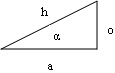
\includegraphics{media/02/image24.png}
\caption{Right Triangle}
\end{figure}

For any right triangle with hypotenuse \(h\), an acute angle \(\alpha\), side length \(o\) opposite from \(\alpha\), and side length \(a\) adjacent to \(\alpha\), the following terms are defined:

\begin{align}
\text{sine } \alpha &= \sin{\alpha} = \frac{o}{h} \\
\text{cosine } \alpha &= \cos{\alpha} = \frac{a}{h} \\
\text{tangent } \alpha &= \tan{\alpha} = \frac{o}{a} = \frac{\sin{\alpha}}{cos{\alpha}} \\
\text{cotangent } \alpha &= \cot{\alpha} = \text{ctn } \alpha = \frac{a}{o} = \frac{1}{\tan{\alpha}} = \frac{\cos{\alpha}}{\sin{\alpha}} \\
\text{secant } \alpha &= \sec{\alpha} = \frac{h}{a} = \frac{1}{\cos{\alpha}} \\
\text{cosecant } \alpha &= \csc{\alpha} = \frac{h}{o} = \frac{1}{\sin{\alpha}} \\
\text{exsecant } \alpha &= \text{exsec } \alpha = \sec{\alpha} - 1 \\
\text{versine } \alpha &= \text{vers } \alpha = 1 - \cos{\alpha} \\
\text{coversine } \alpha &= \text{covers } \alpha = 1 - \sin{\alpha} \\
\text{haversine } \alpha &= \text{hav } \alpha = \frac{\text{vers } \alpha}{2} \\
\end{align}

also defined are the following\ldots{}

\begin{align}
\text{hyperbolic sine of } x &= \sinh{x} = \frac{\mathrm{e}^x - \mathrm{e}^{-x}}{2} \\
\text{hyperbolic cosine of } x &= \cosh{x} = \frac{\mathrm{e}^x + \mathrm{e}^{-x}}{2} \\
\text{hyperbolic tangent of } x &= \tanh{x} = \frac{\sinh{x}}{\cosh{x}} = \frac{\mathrm{e}^x - \mathrm{e}^{-x}}{\mathrm{e}^x + \mathrm{e}^{-x}} \\
\text{csch } x &= \frac{1}{\sinh{x}} \\
\text{sech } x &= \frac{1}{\cosh{x}} \\
\text{coth } x &= \frac{1}{\tanh{x}} \\
\end{align}

\hypertarget{identities-1}{%
\subsection*{Identities}\label{identities-1}}
\addcontentsline{toc}{subsection}{Identities}

\hypertarget{pythagorean-identities}{%
\subsubsection*{Pythagorean Identities:}\label{pythagorean-identities}}
\addcontentsline{toc}{subsubsection}{Pythagorean Identities:}

\begin{align}
\sin^2{\alpha} + \cos^2{\alpha} &= 1 \\
1 + \tan^2{\alpha} &= \sec^2{\alpha} \\
1 + \cot^2{\alpha} &= \csc^2{\alpha} \\
\end{align}

\hypertarget{half-angle-identities}{%
\subsubsection*{Half Angle Identities:}\label{half-angle-identities}}
\addcontentsline{toc}{subsubsection}{Half Angle Identities:}

\begin{align}
\sin{\frac{\alpha}{2}} &= \pm \sqrt{\frac{1 - \cos{\alpha}}{2}} \text{ (negative if } \frac{\alpha}{2} \text{ is in quadrant III or IV)}\\
\cos{\frac{\alpha}{2}} &= \pm \sqrt{\frac{1 + \cos{\alpha}}{2}} \text{ (negative if } \frac{\alpha}{2} \text{ is in quadrant II or III)}\\
\tan{\frac{\alpha}{2}} &= \pm \sqrt{\frac{1 - \cos{\alpha}}{1 + \cos{\alpha}}} \text{ (negative if } \frac{\alpha}{2} \text{ is in quadrant II or IV)}\\
\end{align}

\hypertarget{double-angle-identities}{%
\subsubsection*{Double-Angle Identities:}\label{double-angle-identities}}
\addcontentsline{toc}{subsubsection}{Double-Angle Identities:}

\begin{align}
\sin{2\alpha} &= 2\sin{\alpha}\cos{\alpha}\\
\cos{2\alpha} &= 2\cos^2{\alpha} - 1 = 1 - 2\sin^2{\alpha} = \cos^2{\alpha} - \sin^2{\alpha}\\
\tan{2\alpha} &= \frac{2\tan{\alpha}}{1 - \tan^2{\alpha}}\\
\end{align}

\hypertarget{n-angle-identities}{%
\subsubsection*{n-Angle Identities:}\label{n-angle-identities}}
\addcontentsline{toc}{subsubsection}{n-Angle Identities:}

\begin{align}
\sin{3\alpha} &= 3\sin{\alpha} - 4\sin^3{\alpha}\\
\cos{3\alpha} &= 4\cos^3{\alpha} - 3\cos{\alpha}\\
\sin{n\alpha} &= 2\sin\big(\left(n-1\right)\alpha\big) \cos{\alpha} - \sin(n-2)\alpha\\
\cos{n\alpha} &= 2\cos\big(\left(n-1\right)\alpha\big) \cos{\alpha} - \cos\left(n-2\right)\alpha\\
\end{align}

\hypertarget{two-angle-identities}{%
\subsubsection*{Two-Angle Identities:}\label{two-angle-identities}}
\addcontentsline{toc}{subsubsection}{Two-Angle Identities:}

\begin{align}
\sin\left(\alpha + \beta\right) &= \sin{\alpha}\cos{\beta} + \cos{\alpha}\sin{\beta}\\
\cos\left(\alpha + \beta\right) &= \cos{\alpha}\cos{\beta} - \sin{\alpha}\sin{\beta}\\
\tan\left(\alpha + \beta\right) &= \frac{\tan{\alpha} + \tan{\beta}}{1 - \tan{\alpha}\tan{\beta}}\\
\sin\left(\alpha - \beta\right) &= \sin{\alpha}\cos{\beta} - \cos{\alpha}\sin{\beta}\\
\cos\left(\alpha - \beta\right) &= \cos{\alpha}\cos{\beta} + \sin{\alpha}\sin{\beta}\\
\tan\left(\alpha - \beta\right) &= \frac{\tan{\alpha} - \tan{\beta}}{1 + \tan{\alpha}\tan{\beta}}\\
\end{align}

\hypertarget{sum-and-difference-identities}{%
\subsubsection*{Sum and Difference Identities:}\label{sum-and-difference-identities}}
\addcontentsline{toc}{subsubsection}{Sum and Difference Identities:}

\begin{align}
\sin{\alpha} + \sin{\beta} &=  2\sin{\frac{\alpha + \beta}{2}}\cos{\frac{\alpha - \beta}{2}}\\
\sin{\alpha} - \sin{\beta} &=  2\cos{\frac{\alpha + \beta}{2}}\sin{\frac{\alpha - \beta}{2}}\\
\cos{\alpha} + \cos{\beta} &=  2\cos{\frac{\alpha + \beta}{2}}\sin{\frac{\alpha - \beta}{2}}\\
\cos{\alpha} - \cos{\beta} &= -2\cos{\frac{\alpha + \beta}{2}}\sin{\frac{\alpha - \beta}{2}}\\
\tan{\alpha} + \tan{\beta} &=  \frac{\sin\left(\alpha + \beta\right)}{\cos{\alpha}\cos{\beta}}\\
\cot{\alpha} + \cot{\beta} &=  \frac{\sin\left(\alpha + \beta\right)}{\sin{\alpha}\sin{\beta}}\\
\tan{\alpha} - \tan{\beta} &=  \frac{\sin\left(\alpha - \beta\right)}{\cos{\alpha}\cos{\beta}}\\
\cot{\alpha} - \cot{\beta} &= -\frac{\sin\left(\alpha - \beta\right)}{\sin{\alpha}\sin{\beta}}\\
\sin^2{\alpha} - \sin^2{\beta} &=  \sin\left(\alpha + \beta\right) \sin\left(\alpha - \beta\right)\\
\cos^2{\alpha} - \cos^2{\beta} &= -\sin\left(\alpha + \beta\right) \sin\left(\alpha - \beta\right)\\
\cos^2{\alpha} - \sin^2{\beta} &=  \cos\left(\alpha + \beta\right) \cos\left(\alpha - \beta\right)\\
\end{align}

\hypertarget{power-identities}{%
\subsubsection*{Power Identities:}\label{power-identities}}
\addcontentsline{toc}{subsubsection}{Power Identities:}

\begin{align}
\sin{\alpha}\sin{\beta} &= \frac{\cos\left(\alpha - \beta\right) - \cos\left(\alpha + \beta\right)}{2}\\
\cos{\alpha}\cos{\beta} &= \frac{\cos\left(\alpha - \beta\right) + \cos\left(\alpha + \beta\right)}{2}\\
\sin{\alpha}\cos{\beta} &= \frac{\sin\left(\alpha + \beta\right) + \sin\left(\alpha - \beta\right)}{2}\\
\cos{\alpha}\sin{\beta} &= \frac{\sin\left(\alpha + \beta\right) - \sin\left(\alpha - \beta\right)}{2}\\
\tan{\alpha}\cot{\alpha} &= \sin{\alpha}\csc{\alpha} = \cos{\alpha}\sec{\alpha} = 1\\
\sin^2{\alpha} &= \frac{1 - \cos{2\alpha}}{2}\\
\cos^2{\alpha} &= \frac{1 + \cos{2\alpha}}{2}\\
\sin^3{\alpha} &= \frac{3\sin{\alpha} - \sin{3\alpha}}{4}\\
\cos^3{\alpha} &= \frac{3\cos{\alpha} + \cos{3\alpha}}{4}\\
\sin^4{\alpha} &= \frac{3 - 4\cos{2\alpha} + \cos{4\alpha}}{8}\\
\cos^4{\alpha} &= \frac{3 + 4\cos{2\alpha} + \cos{4\alpha}}{8}\\
\sin^5{\alpha} &= \frac{10\sin{\alpha} - 5\sin{3\alpha} + \sin{5\alpha}}{16}\\
\cos^5{\alpha} &= \frac{10\cos{\alpha} + 5\cos{3\alpha} + \cos{5\alpha}}{16}\\
\end{align}

\hypertarget{oblique-triangles}{%
\subsubsection*{OBLIQUE TRIANGLES}\label{oblique-triangles}}
\addcontentsline{toc}{subsubsection}{OBLIQUE TRIANGLES}

(no right angle, angles A,B,C are opposite of legs a,b,c)

\begin{figure}
\centering
\includegraphics{media/02/image25.png}
\caption{Oblique Triangle}
\end{figure}

\hypertarget{law-of-sines}{%
\paragraph*{Law of Sines:}\label{law-of-sines}}
\addcontentsline{toc}{paragraph}{Law of Sines:}

\[\frac{a}{\sin{A}} = \frac{b}{\sin{B}} = \frac{c}{\sin{C}}\]

\hypertarget{law-of-cosines}{%
\paragraph*{Law of Cosines:}\label{law-of-cosines}}
\addcontentsline{toc}{paragraph}{Law of Cosines:}

\begin{align}
a^2  &= b^2  + c^2  - 2bc\cos{A}\\
b^2  &= a^2  + c^2  - 2ac\cos{B}\\
c^2  &= a^2  + b^2  - 2ab\cos{C}\\
\cos{C} &= \frac{a^2 +b^2 -c^2}{2ab}\\
\end{align}

\hypertarget{law-of-tangents}{%
\paragraph*{Law of Tangents:}\label{law-of-tangents}}
\addcontentsline{toc}{paragraph}{Law of Tangents:}

\[\frac{a-b}{a+b} = \frac{\tan\frac{a-b}{2}}{\tan\frac{a+b}{2}}\]

\hypertarget{projection-formulas}{%
\paragraph*{Projection Formulas:}\label{projection-formulas}}
\addcontentsline{toc}{paragraph}{Projection Formulas:}

\begin{align}
a &= b\cos{C} + c\cos{B}\\
b &= c\cos{A} + a\cos{C}\\
c &= a\cos{B} + b\cos{A}\\
\end{align}

\hypertarget{mollweides-check-formulas}{%
\paragraph*{Mollweide's Check Formulas:}\label{mollweides-check-formulas}}
\addcontentsline{toc}{paragraph}{Mollweide's Check Formulas:}

\begin{align}
\frac{a-b}{c} &= \frac{\sin\frac{A-B}{2}}{\cos\frac{C}{2}}\\
\frac{a+b}{c} &= \frac{\cos\frac{A-B}{2}}{\sin\frac{C}{2}}\\
\end{align}

\hypertarget{matrix-algebra}{%
\section{Matrix Algebra}\label{matrix-algebra}}

\hypertarget{fundamentals}{%
\subsection{Fundamentals}\label{fundamentals}}

(reference 2.5)

Given two matrices, \(A, B\) where \(A\) is an \(i \times m\) matrix and \(B\) is an \(m \times j\) matrix, that is, the numbers of columns of the first matrix equals the number of rows of the second matrix, we define matrix multiplication as follows:
\[A \times B = A B = C\] where the entry in the \emph{i}th row and \emph{j}th column is given by \(c_{ij}\) where:
\[c_{ij} = \sum_{k=1}^m (a_{ik}b_{kj}).\]
In other words, we take the dot product of the \emph{i}th row and the \emph{j}th column.

For example, the product of a pair of, \(2 \times 2\) matrices is:

\[
\begin{bmatrix} 
a_{11} & a_{12} \\ 
a_{21} & a_{22} 
\end{bmatrix} 
\begin{bmatrix} 
b_{11} & b_{12} \\ 
b_{21} & b_{22} 
\end{bmatrix} 
= 
\begin{bmatrix} 
a_{11}b_{11}+a_{12}b_{21} & a_{11}b_{12}+a_{12}b_{22} \\ 
a_{21}b_{11}+a_{22}b_{21} & a_{21}b_{12}+a_{22}b_{22} 
\end{bmatrix} 
\]

The \emph{identity} matrix \(I\) occupies the same position in matrix algebra that the value of unity does in ordinary algebra. It is a square matrix consisting of ones on the principle diagonal and zeros everywhere else:
\[I =
\begin{bmatrix}
1 & 0 & \dots & 0 \\
0 & 1 & \dots & 0 \\
\vdots & \vdots & \ddots & \vdots\\
0 & 0 & \dots & 1
\end{bmatrix}
\]

For any matrix \(A\), \(A I = I A = A\).

The \emph{inverse} matrix \(A^{-1}\), if it exists, is the multiplicative inverse under matrix multiplication. That is,
\[A A^{-1} = A^{-1}A = I.\]

\hypertarget{cofactors-and-determinants}{%
\subsection{Cofactors and Determinants}\label{cofactors-and-determinants}}

We denote the \emph{determinant} of a square matrix by \(|A|\). For a two-by-two matrix, the determinant is as follows:
\[
\begin{vmatrix}
a & b \\
c & d
\end{vmatrix} = ad - bc.
\]

Formally, for any \(n \times n\) matrix, the determinant is:
\[|A| = \sum_{i=1}^{k}a_{ij} C_{ij} \] where
\[C_{ij} = (-1)^{i+j}M_{ij}\] where
the minor matrix \(M_{ij}\) is in the \((n-1) \times (n-1)\) matrix resulting when the \emph{i}th row and \emph{j}th column are removed from \(A\). This holds when the sum above is taken over any row, \(i\), or column \(j\). The \emph{cofactor} is \(C_{ij}\) above.

Arbitrarily expanding about the first row of a 3 x 3 matrix gives the determinant:

\[|A| = (-1)^{1+1} a_{11} \begin{vmatrix}
a_{22} & a_{23} \\
a_{32} & a_{33}
\end{vmatrix} 
+ (-1)^{1+2}a_{12} \begin{vmatrix}
a_{21} & a_{23} \\
a_{22} & a_{33}
\end{vmatrix} 
+ (-1)^{1+3}a_{13}\begin{vmatrix}
a_{21} & a_{22} \\
a_{22} & a_{23}
\end{vmatrix}.\]

\hypertarget{computing-the-inverse-of-a-matrix}{%
\subsection{Computing the Inverse of a Matrix}\label{computing-the-inverse-of-a-matrix}}

There is a straightforward (but computationally inefficient and intensive) four-step method for computing the \emph{inverse} of a matrix \(A\).

\textbf{Step 1} Compute the determinant of \(A\). If the determinant is zero or does not exist, the matrix is said to be \emph{singular} and an inverse does not exist.

\textbf{Step 2} Transpose matrix \(A\), denoted \(A^T\).

\textbf{Step 3} Replace each element \(a_{ij}\) of the transposed matrix by its \emph{cofactor}, \(A_{ij}\). The resulting matrix is called the \emph{adjoint} matrix, \(adj\left[A\right]\).

\textbf{Step 4} Divide the adjoint matrix by the determinant.

\emph{Example.} Solve the following set of simultaneous equations.
\[
3x_1 + 2x_2 - 2x_3 = y_1 \\
-x_1 +x_2 +4x_3 = y_2 \\
2x_1 -3x_2 +4x_3 = y_3
\]
We can express this as \(Ax = y\). If the matrix is invertible, then the solution of the system is given by \(x = A^{-1} y\).

\textbf{Step 1.} Compute the determinant: \(|A| = 70\).

\textbf{Step 2.} Transpose the matrix.
\[
A^T = \begin{bmatrix} 
3 & -1 & -2 \\ 
2 & 1 & -3 \\
-2 & 4 & 4
\end{bmatrix} 
\]

\textbf{Step 3.} Determine the adjoint matrix by replacing each element in \(A^T\) by its Cofactor.

\[
  adj\left[A\right] =
\begin{bmatrix}
\begin{vmatrix} 1 & -3 \\ 4 & 4 \end{vmatrix} 
& - \begin{vmatrix} 2 & -3 \\ -2 & 4 \end{vmatrix}  
& \begin{vmatrix} 2 & 1 \\ -2 & 4 \end{vmatrix} \\
- \begin{vmatrix} -1 & 2 \\ 4 & 4 \end{vmatrix} 
& \begin{vmatrix} 3 & 2 \\ -2 & 4 \end{vmatrix}  
& - \begin{vmatrix} 3 & -1 \\ -2 & 4\end{vmatrix} \\
\begin{vmatrix} -1 & 2 \\ 1 & -3 \end{vmatrix} 
& - \begin{vmatrix} 3 & 2 \\ 2 & -3 \end{vmatrix}  
& \begin{vmatrix} 3 & -1 \\ 2 & 1\end{vmatrix} \\
\end{bmatrix}
=
\begin{bmatrix}
16 & -2 & 10 \\
12 & 16 & -10 \\
1 & 13 & 5 \\
\end{bmatrix}
\]

\textbf{Step 4.} Divide by the determinant.

\[
\left[ A \right]^{-1} = \frac{1}{70}
\begin{bmatrix}
16 & -2 & 10 \\
12 & 16 & -10 \\
1 & 13 & 5 \\
\end{bmatrix}
\]

Then, if \(y_1 = 1, y_2 = 13\), and \(y_3 = 8\):

\[
\begin{bmatrix} x_1 \\ x_2 \\ x_3 \end{bmatrix} = \frac{1}{70}
\begin{bmatrix}
16 & -2 & 10 \\
12 & 16 & -10 \\
1 & 13 & 5 \\
\end{bmatrix}
\begin{bmatrix}
1 \\ 13 \\ 8
\end{bmatrix} 
\]

\begin{align}
x_1 &= \frac{1}{70} \left( 16 - 26 + 80 \right) = \frac{70}{70} &= 1 \\
x_2 &= \frac{1}{70} \left( 12 0 208 - 80 \right) = \frac{140}{70} &= 2 \\
x_3 &= \frac{1}{70} \left( 1 + 169 + 40 \right) = \frac{210}{70} &= 3 \\
\end{align}

\hypertarget{cramers-rule}{%
\subsection{Cramer's Rule}\label{cramers-rule}}

Given a matrix, \(A\) and vectors, \(x, b\), we have a system of equations \(A x = b\). If the determinant of the matrix exists, then let \(A_r\) be the matrix obtained from \(A\) by replacing the \(r\)th column with the vector \(b\). Then the system of equations has a unique solution:
\[x_r = \det(A)/ \det(A_r).\]

Example of Cramer's Rule

\[
\begin{bmatrix}
1 & 0 & 2\\
-3 & 4 & 6 \\
-1 & -2 & 3 \\
\end{bmatrix}
\begin{bmatrix}
x_1 \\ x_2 \\ x_3
\end{bmatrix}
=
\begin{bmatrix}
6 \\ 30 \\ 8
\end{bmatrix}
\]

\begin{align}
A &= \begin{bmatrix} 1 & 0 & 2 \\ -3 & 4 & 6 \\ -1 & -2 & 3 \end{bmatrix} & A_1 = \begin{bmatrix} 6 & 0 & 2 \\ 30 & 4 & 6 \\ 8 & -2 & 3 \end{bmatrix} \\
A_2 &= \begin{bmatrix} 1 & 6 & 2 \\ -3 & 30 & 6 \\ -1 & 8 & 3 \end{bmatrix} & A_3 = \begin{bmatrix} 1 & 0 & 6 \\ -1 & 4 & 30 \\ -3 & -2 & 8 \end{bmatrix} \\
\end{align}

\begin{align}
x_1 &= \frac{\det\left( A_1 \right)}{\det\left( A \right)} = \frac{-40}{44} = \frac{-10}{11} \\
x_2 &= \frac{\det\left( A_2 \right)}{\det\left( A \right)} = \frac{72}{44} = \frac{18}{11} \\
x_3 &= \frac{\det\left( A_3 \right)}{\det\left( A \right)} = \frac{152}{44} = \frac{38}{11} \\
\end{align}

\hypertarget{vector-algebra}{%
\section{Vector Algebra}\label{vector-algebra}}

(reference 2.5)

\hypertarget{addition}{%
\subsection{Addition}\label{addition}}

Given vectors \(\bar{A}\) and \(\bar{B}\), where the \(i\)th component of \(\bar{A}\) is given by \(a_i\), we define addition \(\bar{A} + \bar{B}\) component-wise, such that the \(i\)th component of \(\bar{A} + \bar{B}\) is given by \(a_i + b_i\).

\begin{figure}
\centering
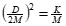
\includegraphics{media/02/image39.png}
\caption{Vector Addition}
\end{figure}

\hypertarget{subtraction}{%
\subsection{Subtraction}\label{subtraction}}

We define vector subtraction just as we defined vector addition above.

\begin{figure}
\centering
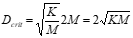
\includegraphics{media/02/image40.png}
\caption{Vector Subtraction}
\end{figure}

\hypertarget{scalar-multiplication}{%
\subsection{Scalar Multiplication}\label{scalar-multiplication}}

Given a real number, \(m\), and vectors \(\bar{A}\) and \(\bar{B}\), where the \emph{i}th component of \(\bar{A}\) is given by \(a_i\), we define scalar multiplication \(m \bar{A}\) component-wise, such that the \emph{i}th component of \(m \bar{A}\) is given by \(m a_i\).

When \(m\) and \(a+i\) are real numbers, the usual properties apply:

\textbf{Commutative} \(m \bar{A} = \bar{A} m\).

\textbf{Associative} \(m (n \bar{A}) = (mn) \bar{A}\).

\textbf{Distributive} \((m + n) \bar{A} = m \bar{A} + n \bar{A}\).

When \(a+i\) are real numbers, we have the following properties that apply to \emph{vectors}:

\textbf{Commutative} \(\bar{A} + \bar{B} = \bar{B} + \bar{A}\).

\textbf{Associative} \(\bar{A} + (\bar{B} + \bar{C}) = (\bar{A} + \bar{B}) + \bar{C}\).

\textbf{Distributive} \(m (\bar{A} + \bar{B}) = m \bar{A} + m \bar{B}\).

\hypertarget{dot-product}{%
\subsection{Dot Product}\label{dot-product}}

Given vectors \(\bar{A}\) and \(\bar{B}\), where the \(i\)th component of \(\bar{A}\) is given by \(a_i\) and the vectors have the same dimension, \(n\), we define the dot product \(\bar{A} \cdot \bar{B}\) as follows:
\[\bar{A} \cdot \bar{B} = \sum_{i=1}^{n}a_i b_i .\]
For example, given three-dimensional vectors, we have:
\[\bar{A} \cdot \bar{B} = a_1 b_1 + a_2 b_2 + a_3 b_3 .\]
The terms dot product, scalar product, and inner product usually mean the same thing.

\hypertarget{norm}{%
\subsection{Norm}\label{norm}}

The norm or vector norm, denoted
\[ \left| \bar{A} \right|,\]
is the magnitude of the vector. We compute it thus:
\[ \left| \bar{A} \right| = \sqrt{\sum_{i=1}^{n} a_i^2} .\].
For example, given a three-dimensional vector in the \(xyz\) plane, we have:
\[ \left| \bar{A} \right| = \sqrt{a_x^2 + a_y^2 + a_z^2} .\]
The two types of notation, \(| \bar{A} |\) and \(|| \bar{A} ||\) are equivalent.

With this additional notation, we can also define the \textbf{dot product} this way:
\[\bar{A} \cdot \bar{B} = \left| \bar{A} \right| \left| \bar{B} \right| \cos{\theta} ,\]
where \(\theta\) is the angle between the vectors.

\hypertarget{vector-cross-product}{%
\subsection{Vector Cross Product}\label{vector-cross-product}}

The cross product is an operation on vectors in three dimensional space denoted \(\bar{A} \times \bar{B} .\) We can define it in terms of matrix determinants in the following way.
\[ \bar{A} \times \bar{B} = \begin{vmatrix}
\hat{i} & \hat{j} & \hat{k}\\
a_x & a_y & a_z\\
b_x & b_y & b_z
\end{vmatrix}
.\]

Expanding this expression gives us:
\[ \bar{A} \times \bar{B} = \begin{vmatrix}
a_y & a_z\\
b_y & b_z
\end{vmatrix} \hat{i}
+ \begin{vmatrix}
a_x & a_z\\
b_x & b_z
\end{vmatrix} \hat{j}
+ \begin{vmatrix}
a_x & a_y\\
b_x & b_y
\end{vmatrix} \hat{k}
.\]

\begin{figure}
\centering
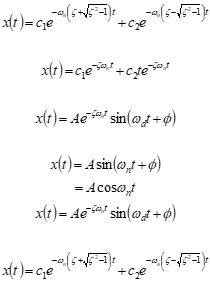
\includegraphics{media/02/image49.png}
\caption{Cross Product}
\end{figure}

\[\hat{i} \times \hat{i} = \hat{j} \times \hat{j} = \hat{k} \times \hat{k} = 0 \]
\[\hat{i} \times \hat{j} = \hat{k} \quad \hat{j} \times \hat{k} = \hat{i} \quad \hat{k} \times \hat{i} = \hat{j} \]
\[\hat{j} \times \hat{i} = -\hat{k} \quad \hat{k} \times \hat{j} = -\hat{i} \quad \hat{i} \times \hat{k} = -\hat{j} \]

\hypertarget{vector-differentiation}{%
\subsection{Vector Differentiation}\label{vector-differentiation}}

Let \(\vec{r}(t)\) be a vector-valued function, denoted in this way: \(\vec{r}(t) = (x(t),y(t))\), which is an example of a function that returns a position vector. A similar and equivalent notation is as follows: \(\vec{r}(t) = x(t)\hat{i} + y(t)\hat{j}\).

The first derivative of \(\vec{r}(t)\) with respect to time, \(t\), is a vector-valued function that denotes velocity. This function returns a vector tangential to the trajectory with a magnitude equal to the speed of the particle.

The second derivative of \(\vec{r}(t)\) with respect to time, \(t\), is a vector-valued function that denotes acceleration. This function returns a vector tangential to the velocity vector with a magnitude equal to the acceleration of the particle.

With this notation, the normal differenation operations hold for vector-valued \emph{functions} along with the following.

\textbf{Derivative of a Sum}
\[\frac{d}{dt}\left( \vec{r}(t) + \vec{s}(t) \right) = \frac{d}{dt}\vec{r}(t) + \frac{d}{dt}\vec{s}(t).\]

\textbf{Derivative of a Dot Product}
\[\frac{d}{dt}\left( \vec{r}(t) \cdot \vec{s}(t) \right) = \vec{r}(t) \cdot \frac{d}{dt}\vec{s}(t) + \frac{d}{dt}\vec{r}(t) \cdot \vec{s}(t).\]

\textbf{Derivative of a Cross Product}
\[\frac{d}{dt}\left( \vec{r}(t) \times \vec{s}(t) \right) = \vec{r}(t) \times \frac{d}{dt}\vec{s}(t) +  \frac{d}{dt}\vec{r}(t) \times \vec{s}(t).\]

\textbf{Derivative of a Scalar Product}
If \(f(t)\) is a scalar-valued function, then
\[\frac{d}{dt}\left( f(t)\vec{r}(t) \right) = f(t)\frac{d}{dt}\vec{r}(t) + \left(\frac{d}{dt} f(t)\right) \vec{r}(t).\]

\hypertarget{motion-of-a-point-using-two-reference-systems}{%
\subsection{Motion of a point using two reference systems}\label{motion-of-a-point-using-two-reference-systems}}

Reference A can be considered the inertial frame while Rotation of the B reference relative to the A reference must be considered when observing motion with respect to the A reference system.

\begin{figure}
\centering
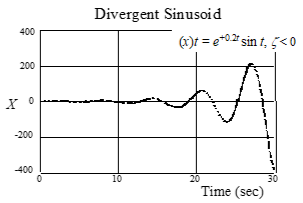
\includegraphics{media/02/image52.png}
\caption{Trajectory with Two Reference Systems}
\end{figure}

Note: Unit vectors are along the B system axes. Subscripts denote reference system. Reference B can be equivalent to a maneuvering aircraft.

\[\bar{\rho} = x \hat{i} + y \hat{j} + z \hat{k}\]

\[\left( \frac{d \bar{\rho}}{dt} \right)_B = \dot{x} \hat{i} + \dot{y} \hat{j} + \dot{z} \hat{k}\]

\[\left( \frac{d \bar{\rho}}{dt} \right)_A = \left( \dot{x}\hat{i} + \dot{y}\hat{j} + \dot{z}\hat{k} \right) + \left( x \dot{\hat{i}} + y \dot{\hat{j}} + z \dot{\hat{k}} \right)\]

\[\left( \frac{d \bar{\rho}}{dt} \right)_A = \left( \frac{d \bar{\rho}}{dt} \right)_B + \bar{\omega} \times \bar{\rho}\]

The velocities of the particle \(P\) relative to the \(A\) and to the \(B\) references, respectively, are as follows:

\[\bar{V}_A = \left( \frac{d\bar{r}}{dt} \right)_A\]

\[\bar{V}_B = \left( \frac{d\bar{\rho}}{dt} \right)_B\]

These velocities can be related by noting that \(\bar{r} = \bar{R} + \bar{\rho}\).

Taking the derivative with respect to time for the \(A\) reference:
\[\bar{V}_A = \left(\frac{d \bar{r}}{dt}  \right)_A = \left( \frac{d \bar{R}}{dt} \right)_A + \left( \frac{d \bar{\rho}}{dt} \right)_A\]

The term \(\left(\frac{d \bar{r}}{dt} \right)_A\) is the velocity of the origin of \(B\) reference relative to the \(A\) reference. We denote
\[\left(\frac{d \bar{r}}{dt}  \right)_A = \dot{\overline{R}}.\]

Substituting for \(\left( \frac{d \bar{\rho}}{dt} \right)_A\) gives the following:
\[\bar{V}_A  = \dot{\overline{R}} + \bar{V}_B + \bar{\omega} \times \bar{\rho}.\]

The term is the ``transport velocity'' and is the only velocity if point P is rigidly attached to reference B.

A similar derivation for acceleration gives the following:
\[\bar{a}_A = \bar{a}_B + 2(\bar{\omega} \times \bar{V}_B) + \ddot{\overline{R}} + (\dot{\bar{\omega}} \times \bar{\rho}) + \bar{\omega} \times (\bar{\omega} \times \bar{\rho}).\]

Here \(\bar{\omega} \times (\bar{\omega} \times \bar{\rho})\) is the centripetal acceleration, \(2(\bar{\omega} \times \bar{V}_B)\) is the Coriolis acceleration, and the transport acceleration, which is the only acceleration if point P is rigidly attached to reference B, is given by the following:
\[\ddot{\overline{R}} + (\dot{\bar{\omega}} \times \bar{\rho}) + \bar{\omega} \times (\bar{\omega} \times \bar{\rho}).\]

\hypertarget{motion-of-a-point-using-one-reference-system}{%
\subsection{Motion of a point using one reference system}\label{motion-of-a-point-using-one-reference-system}}

Reference A can be considered the inertial frame while the body can be equivalent to a maneuvering aircraft.

\begin{figure}
\centering
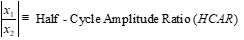
\includegraphics{media/02/image65.png}
\caption{Motion with One Reference System}
\end{figure}

A derivation similar to the previous gives us the following for
velocity:
\[\dot{\bar{\rho}} = \bar{\omega} \times \bar{\rho},\]

and acceleration:
\[\bar{a}_b = \bar{a}_a + (\dot{\bar{\omega}} \times \bar{\rho}) + \bar{\omega} \times (\bar{\omega} \times \bar{\rho}).\]

\hypertarget{probability-and-statistics}{%
\section{Probability and Statistics}\label{probability-and-statistics}}

(reference 2.6)

\textbf{\emph{Definitions:}}

Population: The set of all possible observations

Sample: Any subset of a population

Homogeneous Sample: The sample comes from 1 population only

Random Sample: Equal probability of selecting any member of the population

Independence (of events A and B): P(A and B) = P(A)*P(B)

Sample and Population Mean (Average value):
\[\mu = \bar{x} = \frac{1}{N} \sum_{i=1}^N{x_i} \]

Mode (Most commonly occurring value in a sample)

Median (middle value, 50th percentile. Half of the sample values are greater and half are smaller)

Deviation:
\[d_i = x_i - \bar{x} \]

Population Variance:
\[\sigma^2 =  \frac{1}{N} \sum_{i=1}^N{(x_i - \bar{x}})^2 = \frac{1}{N} \sum_{i=1}^N{d_i^2}\]

Population Standard Deviation (square root of variance):
\[\sigma = \sqrt{\frac{1}{N} \sum_{i=1}^N{(x_i - \bar{x}})^2} \]

Sample Standard Deviation:
\[s = \sqrt{\frac{1}{N-1} \sum_{i=1}^N{(x_i - \bar{x}})^2} \]

\textbf{\emph{Discrete Probability Distributions:}}

\textbf{\emph{Uniform}}
The probability of any outcome in a given set is the same. If there are \(N\) possible outcomes in a set, then the probability of a given outcome is \(p=1/N\). For example, when rolling a fair dice with \(N=6\) sides, the probability that the toss will result in any given side is \(p = 1/6\).

\textbf{\emph{Binomial}}
The probability that the random variable \(X = x\) in \(N\) independent events, each having probability \(p\) of success, and \(1-p\) of failure.
\[P(X = k) = \binom{N}{k}p^x (1-p)^{N-x}\] where
\[\binom{N}{k} = \frac{N!}{k!(N-k)!}.\]

For example, tossing a fair coin N times where \(p = 1/2\) is the probability of getting a head on any toss. If \(X\) indicates the number of heads in \(N\) tosses, then we have \(P(X = x) = (1/2)^x (1/2)^{N-x}\). For \(N = 4\) we have the following table:

\begin{longtable}[]{@{}cc@{}}
\toprule
x & P(X=x)\tabularnewline
\midrule
\endhead
\(0\) & \(1/16\)\tabularnewline
\(1\) & \(1/4\)\tabularnewline
\(2\) & \(3/8\)\tabularnewline
\(3\) & \(1/4\)\tabularnewline
\(4\) & \(1/16\)\tabularnewline
\bottomrule
\end{longtable}

\textbf{Continuous Distributions}
Continuous distributions are defined for all \(x \in [a,b]\), where \(a, b \in \mathbb{R}\) or for all \(x \in (-\infty, \infty)\), that is, the whole real number line. The probability for any single point is zero; that is, \(P(X=x) = 0\). Instead, one must work with probability on an interval, e.g., \(P(0 < x)\) or \(P(a < x < b)\).

\textbf{The Normal Distribution}
The probability density function of the Normal Distribution is given by:
\[f(x) = \frac{1}{\sqrt{2 \pi \sigma}}\mathrm{e}^{\frac{-(x-\mu)^2}{2\sigma^2}}\]

\textbf{The Standard Normal Distribution}
The Standard Normal Distribution is simply the Normal Distribution with \(\mu = 0\) and \(\sigma=1\).

\textbf{Error Probable}
An interval centered at the mean that contains one-half of the distribution.

\textbf{Circular Error Probable}
A circle centered at the mean, in a bivariate normal distribution, that contains one-half of the distribution.

\textbf{Confidence Intervals}
An interval estimate of a statistic.

\textbf{Central Limit Theorem}
The sample mean of data sampled from a normally distributed population is itself normally distributed with mean, \(\mu\), and variance, \(\sigma^2/\sqrt{n}\), where the population distribution is \(N(\mu,\sigma^2)\) and \(n\) is the sample size and usually \(n \geq 30\).

\textbf{Hypothesis Testing} Begins with an assumption (hypothesis), usually about the underlying population distribution of some measured quantity or computed error. Select values for the hypothesis and alternate hypothesis(es) that partition the sample space. Collect N samples of the population test statistic or parameter. There are two types of errors: Type 1 errors reject the hypothesis when it is true; Type II accept the hypothesis when it is false.

\hypertarget{standard-series}{%
\section{Standard Series}\label{standard-series}}

(reference 2.4)

A \emph{Taylor Series} is the expansion of a function about a point, \(a\), given only the value of the function and all of its derivatives at that point. It is used to estimate functions when other analytical techniques will not work.
\[f(x) = \sum_{i=0}^{\infty} \frac{{f(a)(x-a)^i}}{i!} = f(a) + f'(x-a) + \frac{f''(a)(x-a)^2}{2} + \dots + \frac{f^{(n)}(a)(x-a)^n}{n!} + \dots\]

The \emph{Maclaurin Series} is a Taylor Series with \(a = 0\).

The \emph{Binomial Series} is a Taylor Series with \(f(x)=(a + x)^n\). When n is a natural number, the result is a polynomial as follows:
\[(a+x)^n = a^n + na^{n-1}x + \frac{n(n-1)a^{n-2}x^2}{2} + \frac{n(n-1)(n-2)a^{n-3}x^3}{3!} + \dots + x^n\]

The Taylor Series expansion of an \emph{Exponential} function gives the following:
\[a^x = 1 + x \ln a + \frac{(x \ln a)^2}{2} + \frac{(x \ln a)^3}{3!} + \dots\]

In the special case when \(a = e\):
\[\mathrm{e}^x = 1 + x + \frac{x^2}{2} + \frac{x^3}{3!}+ \dots\]

Hyperbolic \(\sin\) and \(\cos\) functions are another special case:
\[\cosh x = \frac{(\mathrm{e}^x + \mathrm{e}^{-x})}{2} = 1 + \frac{x^2}{2} + \frac{x^4}{4!}+ \dots\]
\[\sinh x = \frac{(\mathrm{e}^x - \mathrm{e}^{-x})}{2} = x + \frac{x^3}{3!} + \frac{x^5}{5!}+ \dots\]

The Taylor Series expansion of an \emph{Logarithmic} function gives the following. When \(0 < x < 2\):
\[\ln x = (x-1) - \frac{(x-1)^2}{2} + \frac{(x-1)^3}{3} + \dots\]
When \(x > 1/2\):
\[\ln x = \frac{(x-1)}{x} - \frac{(x-1)^2}{2x^2} + \frac{(x-1)^3}{3x^3} + \dots\]
When \(0 < x\):
\[\ln x = 2 \left[ \frac{(x-1)}{x+1} - \frac{(x-1)^3}{3(x+1)^3} + \frac{(x-1)^5}{5(x-1)^5} + \dots \right]\]

The following are Taylor Series expansion of \emph{Trigonometric} functions:
\[\sin x = x - \frac{x^3}{3!} + \frac{x^5}{5!} -\frac{x^7}{7!}+ \dots\]
\[\cos x = x - \frac{x^2}{2!} + \frac{x^4}{4!} -\frac{x^6}{6!}+ \dots\]
\[\tan x = x + \frac{x^3}{3} + \frac{2x^5}{15} + \frac{17x^7}{315}+ \dots \text{ whenever } (x^2 < \pi^2/4)\]
\[\sin^{-1} x = x + \frac{1}{2}\frac{x^3}{3} + \frac{1}{2}\frac{3}{4}\frac{x^5}{5} + \frac{1}{2}\frac{3}{4}\frac{5}{6}\frac{x^7}{7!} + \dots \text{for } |x|<1\]
\[\cos^{-1} x = \frac{\pi}{2} - \sin^{-1}x \text{ for } |x|<1\]
\[\tan^{-1} x = x - \frac{x^3}{3!} + \frac{x^5}{5!} -\frac{x^7}{7!} + \dots\text{ for } |x|<1\]
\[\ln(\sin x) = \ln x - \frac{x^2}{6} - \frac{x^4}{180} - \frac{x^6}{2835}- \dots \text{for } x^2 < \pi^2\]
\[\ln(\cos x) = - \frac{x^2}{s} - \frac{x^4}{12} - \frac{x^6}{45} - \frac{x^8}{2520} \dots \text{for } x^2 < \frac{\pi^2}{4}\]
\[\ln(\tan x) = \ln x + \frac{x^2}{3} - \frac{7x^4}{90} - \frac{62x^6}{2835}+ \dots \text{for } x^2 < \frac{\pi^2}{4}\]
\[\mathrm{e}^{\sin x} = 1 + x + \frac{x^2}{2!} - \frac{3x^4}{4!} -\frac{8x^5}{5!} + \frac{3x^2}{6!} + \dots\]
\[\mathrm{e}^{\cos x} = e \left(1 - \frac{x^2}{2!} +\frac{4x^2}{4!} - \frac{31x^6}{6!} + \dots \right)\]
\[\mathrm{e}^{\tan x} = 1 + x + \frac{x^2}{2!} + \frac{3x^3}{3!} + \frac{9x^4}{4!} + \frac{37x^5}{5!} + \dots \text{for } x^2 < \frac{\pi^2}{4}\]

\hypertarget{derivative-table}{%
\section{Derivative Table}\label{derivative-table}}

(references 2.2, 2.3)

\begin{itemize}
\tightlist
\item
  \(x\) is the independent variable
\item
  \(u\) and \(v\) are dependent on \(x\)
\item
  \(w\) is dependent on \(u\)
\item
  \(a\) and \(n\) are constants
\item
  \(\log{x}\) is the common logarithm to base 10, \(\log_{10}{x}\)
\item
  \(\ln{x}\) is logarithm to the base \(e\), \(\log_e{x}\)
\end{itemize}

\begin{longtable}[]{@{}l@{}}
\toprule
\endhead
\emph{Fundamental Derivatives}\tabularnewline
\(\frac{da}{dx} = 0\)\tabularnewline
\(\frac{d\left(ax\right)}{dx} = a\)\tabularnewline
\(\frac{dx^n}{dx} = nx^{n-1}\)\tabularnewline
\(\frac{d\left(u + v \right)}{dx} = \frac{du}{dx} + \frac{dv}{dx}\)\tabularnewline
\(\frac{d\left(uv \right)}{dx} = u\frac{dv}{dx} + v\frac{du}{dx}\)\tabularnewline
\(\frac{d\left(\frac{u}{v} \right)}{dx} = \frac{1}{v^2} \left( v\frac{du}{dx} - u\frac{dv}{dx} \right)\)\tabularnewline
\(\frac{dw}{dx} = \frac{dw}{du}\frac{du}{dx}\)\tabularnewline
\(\frac{du^n}{dx} = nu^{n-1}\frac{du}{dx}\)\tabularnewline
\emph{Expressions Containing Exponential and Logarithmic Functions}\tabularnewline
\(\frac{d \ln{x}}{dx} = \frac{1}{x}\)\tabularnewline
\(\frac{d \ln{u}}{dx} = \frac{1}{u}\frac{du}{dx}\)\tabularnewline
\(\frac{d \log{u}}{dx} = \frac{\log{e}}{u}\frac{du}{dx}\)\tabularnewline
\(\frac{d\mathrm{e}^x}{dx} = \mathrm{e}^x\)\tabularnewline
\(\frac{da^x}{dx} = a^x \ln{a}\)\tabularnewline
\(\frac{da^u}{dx} = a^u \ln{a}\frac{du}{dx}\)\tabularnewline
\(\frac{du^v}{dx} = vu^{v-1}\frac{du}{dx} + u^v \ln{u}\frac{dv}{dx}\)\tabularnewline
\emph{Expressions Containing Trigonometric Functions}\tabularnewline
\(\frac{d \sin{x}}{dx} = \cos{x} \text{ or } \frac{d \sin{u}}{dx} = \cos{u}\frac{du}{dx}\)\tabularnewline
\(\frac{d \cos{x}}{dx} = -\sin{x} \text{ or } \frac{d \cos{u}}{dx} = -\sin{u}\frac{du}{dx}\)\tabularnewline
\(\frac{d \tan{x}}{dx} = \sec^2{x} \text{ or } \frac{d \tan{u}}{dx} = \sec^2{u}\frac{du}{dx}\)\tabularnewline
\(\frac{d \sec{x}}{dx} = \sec{x}\tan{x} \text{ or } \frac{d \sec{u}}{dx} = \sec{u}\tan{u}\frac{du}{dx}\)\tabularnewline
\(\frac{d \cot{x}}{dx} = -\csc^2{x} \text{ or } \frac{d \cot{u}}{dx} = -\csc^2{u}\frac{du}{dx}\)\tabularnewline
\(\frac{d \sin^{-1}{x}}{dx} = \frac{1}{\sqrt{1-x^2}} \text{ or } \frac{d \sin^{-1}{u}}{dx} = \frac{1}{\sqrt{1-u^2}}\frac{du}{dx}\)\tabularnewline
\(\frac{d \cos^{-1}{x}}{dx} = -\frac{1}{\sqrt{1-x^2}} \text{ or } \frac{d \cos^{-1}{u}}{dx} = -\frac{1}{\sqrt{1-u^2}}\frac{du}{dx}\)\tabularnewline
\(\frac{d \tan^{-1}{x}}{dx} = \frac{1}{1+x^2} \text{ or } \frac{d \tan^{-1}{u}}{dx} = \frac{1}{1+u^2}\frac{du}{dx}\)\tabularnewline
\(\frac{d \cot^{-1}{x}}{dx} = -\frac{1}{1+x^2} \text{ or } \frac{d \cot^{-1}{u}}{dx} = -\frac{1}{1+u^2}\frac{du}{dx}\)\tabularnewline
\bottomrule
\end{longtable}

\hypertarget{integral-table}{%
\section{Integral Table}\label{integral-table}}

(references 2.2, 2.3)

\begin{itemize}
\tightlist
\item
  \(x\) is any variable
\item
  \(u\) is any function of \(x\)
\item
  \(w\) is dependent on \(u\)
\item
  \(a\) and \(b\) are arbitrary constants
\item
  \(C\), the constant of integration, has been omitted from this table, but
  should be added to the result of every integration
\end{itemize}

\begin{longtable}[]{@{}l@{}}
\toprule
\endhead
\emph{Fundamental Integrals}\tabularnewline
\( \int_{}{} a \, dx = ax \)\tabularnewline
\( \int_{}{} a \, f\left(x\right) dx = a \int_{}{} f\left(x\right) dx \)\tabularnewline
\( \int_{}{} \left(u+v\right) dx = \int_{}{} u\,dx + \int_{}{}v\,dx \)\tabularnewline
\( \int_{}{} u\,dv = uv - \int_{}{}v\,du \)\tabularnewline
\( \int_{}{} \frac{u\,dv}{dx} dx = uv - \int_{}{} v \frac{du}{dx} dx\)\tabularnewline
\( \int_{}{} x^n dx = \frac{x^{n+1}}{n+1} \text{, } n \neq -1\)\tabularnewline
\( \int_{}{} x^{-1} dx = \ln{x}  \)\tabularnewline
\( \int_{}{} w \left( u \right) dx = \int_{}{} w\left( u \right) \frac{dx}{du} u \)\tabularnewline
\( \int_{}{} \frac{dx}{a^2 + x^2} = \frac{1}{a} \tan^{-1} \frac{x}{a} \)\tabularnewline
\( \int_{}{} \frac{dx}{\sqrt{a^2 - x^2}} = \sin^{-1} \frac{x}{a} \)\tabularnewline
\( \int_{}{} \frac{dx}{\sqrt{a^2 \pm x^2}} = \ln \left( x - \sqrt{a^2 \pm x^2} \right) \)\tabularnewline
\( \int_{}{} \sqrt{a^2 - u^2} = \frac{1}{2} \left( u \sqrt{a^2 - x^2} + a^2 \sin^{-1} \frac{u}{a} \right) \)\tabularnewline
\( \int_{}{} \frac{du}{a^2 + u^2} = \frac{1}{a} \tan^{-1} \frac{u}{a} \text{, } a  >  0 \)\tabularnewline
\emph{Expressions Containing Exponential and Logarithmic Functions}\tabularnewline
\( \int_{}{} \frac{dx}{x} = \ln{x} \)\tabularnewline
\( \int_{}{} \mathrm{e}^{x} dx = \mathrm{e}^{x} \)\tabularnewline
\( \int_{}{} \mathrm{e}^{ax} dx = \frac{\mathrm{e}^{ax}}{a} \)\tabularnewline
\( \int_{}{} b^{ax} dx = \frac{b^ax}{a \ln{b}} \)\tabularnewline
\( \int_{}{} \ln{x} dx = x \ln{x} - x \)\tabularnewline
\( \int_{}{} b^{u} du = \frac{b^u}{\ln{u}} \)\tabularnewline
\( \int_{}{} x \mathrm{e}^{ax} dx = \frac{\mathrm{e}^ax}{a^2} \left( ax - 1 \right) \)\tabularnewline
\( \int_{}{} x b^{ax} dx = \frac{x b^{ax}}{a \ln{b} } - \frac{b^{ax}}{a^2 \left( \ln{b} \right) } \)\tabularnewline
\( \int_{}{} x^2 \mathrm{e}^{ax} dx = \frac{\mathrm{e}^{ax}}{a^3} \left(a^2 x^2 - 2ax + 2 \right) \)\tabularnewline
\( \int_{}{} \ln{ax} dx = x \ln{ax} - x \)\tabularnewline
\( \int_{}{} x \ln{ax} dx = \frac{x^2}{2} \ln{ax} - \frac{x^2}{4} \)\tabularnewline
\( \int_{}{} x^2 \ln{ax} dx = \frac{x^3}{3} \ln{ax} - \frac{x^3}{9} \)\tabularnewline
\( \int_{}{} \left( \ln{ax} \right)^2 dx = x \left( \ln{ax} \right)^2 - 2x \ln{ax} + 2x \)\tabularnewline
\( \int_{}{} \frac{dx}{x \ln{ax}} = \ln{\left( \ln{ax} \right)} \)\tabularnewline
\( \int_{}{} \frac{x^n}{\ln{ax}} dx = \frac{1}{a^{n+1}} \int_{}{} \frac{\mathrm{e}^{y} dy}{y} \text{, where } y = \left(n + 1\right) \ln{ax} \)\tabularnewline
\emph{Expressions Containing Trigonometric Functions}\tabularnewline
\( \int_{}{} \sin{x} dx = -\cos{x} \)\tabularnewline
\( \int_{}{} \cos{x} dx = \sin{x} \)\tabularnewline
\( \int_{}{} \tan{x} dx = -\ln{ \left( \cos{x} \right)} \)\tabularnewline
\( \int_{}{} \cot{x} dx = \ln{\left( \sin{x} \right)} \)\tabularnewline
\( \int_{}{} \sec{x} dx = \ln{ \left( \sec{x} + \tan{x} \right)} \)\tabularnewline
\( \int_{}{} \csc{x} dx = \ln{ \left( \csc{x} - \cot{x} \right)} \)\tabularnewline
\( \int_{}{} \sin^2{u} du = \frac{1}{2} u - \frac{1}{2} \sin{u} \cos{u} \)\tabularnewline
\( \int_{}{} \cos^2{u} du = \frac{1}{2} u + \frac{1}{2} \sin{u} \cos{u} \)\tabularnewline
\( \int_{}{} \csc^2{u} du = -\cot{u} \)\tabularnewline
\( \int_{}{} \tan^2{u} du = \tan{u} - u \)\tabularnewline
\( \int_{}{} \cot^2{u} du = -\cot{u} - u \)\tabularnewline
\( \int_{}{} \sin{ax} dx = -\frac{1}{a} \cos{ax} \)\tabularnewline
\( \int_{}{} \sin^2{ax} dx = \frac{x}{2}-\frac{\sin{2ax}}{4a}  \)\tabularnewline
\( \int_{}{} \frac{dx}{\sin{ax}} = \frac{1}{a} \ln{ \tan{\frac{ax}{2}}} \)\tabularnewline
\( \int_{}{} \frac{dx}{\sin^2{ax}} = -\frac{1}{a} \cot{ax} \)\tabularnewline
\( \int_{}{} \frac{dx}{1 \pm \sin{ax}} = \mp \frac{1}{a} \tan{\left( \frac{\pi}{4} \mp \frac{ax}{2} \right) } \)\tabularnewline
\( \int_{}{} \sin{x} \cos{x} dx = \frac{1}{2} \sin^2{x} \)\tabularnewline
\bottomrule
\end{longtable}

\hypertarget{laplace-table}{%
\section{Laplace Table}\label{laplace-table}}

(references 2.2, 2.3)

\begin{longtable}[]{@{}ll@{}}
\toprule
\begin{minipage}[b]{0.42\columnwidth}\raggedright
Time Domain \(f(t) = \mathcal{L}^{-1} \left\{ F \left( s \right) \right\}\)\strut
\end{minipage} & \begin{minipage}[b]{0.52\columnwidth}\raggedright
Frequency Domain \(F\left( s \right) = \mathcal{L} \left\{ f \left( t \right) \right\}\)\strut
\end{minipage}\tabularnewline
\midrule
\endhead
\begin{minipage}[t]{0.42\columnwidth}\raggedright
\[1 \text{ (step function)}\]\strut
\end{minipage} & \begin{minipage}[t]{0.52\columnwidth}\raggedright
\[\frac{1}{s} \text{, where } \left(s >  0\right) \]\strut
\end{minipage}\tabularnewline
\begin{minipage}[t]{0.42\columnwidth}\raggedright
\[t\]\strut
\end{minipage} & \begin{minipage}[t]{0.52\columnwidth}\raggedright
\[\frac{1}{s^2} \text{, where } \left(s >  0\right) \]\strut
\end{minipage}\tabularnewline
\begin{minipage}[t]{0.42\columnwidth}\raggedright
\[t^{n-1}\]\strut
\end{minipage} & \begin{minipage}[t]{0.52\columnwidth}\raggedright
\[\frac{\left( n-1 \right)!}{s^n} \text{, where } \left(s >  0\right) \]\strut
\end{minipage}\tabularnewline
\begin{minipage}[t]{0.42\columnwidth}\raggedright
\[\sqrt{t}\]\strut
\end{minipage} & \begin{minipage}[t]{0.52\columnwidth}\raggedright
\[\frac{{\sqrt \pi  }}{{2{s^{\frac{3}{2}}}}} \text{, where } \left(s >  0\right) \]\strut
\end{minipage}\tabularnewline
\begin{minipage}[t]{0.42\columnwidth}\raggedright
\[\frac{1}{\sqrt{t}}\]\strut
\end{minipage} & \begin{minipage}[t]{0.52\columnwidth}\raggedright
\[\frac{{\sqrt \pi  }}{{{s^{\frac{1}{2}}}}} \text{, where } \left(s >  0\right) \]\strut
\end{minipage}\tabularnewline
\begin{minipage}[t]{0.42\columnwidth}\raggedright
\[{t^{n - \frac{1}{2}}},\,\,\,\,\,n = 1,2,3, \ldots\]\strut
\end{minipage} & \begin{minipage}[t]{0.52\columnwidth}\raggedright
\[\frac{{1 \cdot 3 \cdot 5 \cdots \left( {2n - 1} \right)\sqrt \pi  }}{{{2^n}{s^{n + \frac{1}{2}}}}} {, where } \left(s >  0\right) \]\strut
\end{minipage}\tabularnewline
\begin{minipage}[t]{0.42\columnwidth}\raggedright
\[\mathrm{e}^{at}\]\strut
\end{minipage} & \begin{minipage}[t]{0.52\columnwidth}\raggedright
\[ \frac{1}{s-a} \text{, where } \left(s >  a \right) \]\strut
\end{minipage}\tabularnewline
\begin{minipage}[t]{0.42\columnwidth}\raggedright
\[t\mathrm{e}^{at}\]\strut
\end{minipage} & \begin{minipage}[t]{0.52\columnwidth}\raggedright
\[\frac{1}{{\left( {s - a} \right)}^{2}} \text{, where } \left(s >  a \right) \]\strut
\end{minipage}\tabularnewline
\begin{minipage}[t]{0.42\columnwidth}\raggedright
\[{t^n}{{e}^{at}},\,\,\,\,\,n = 1,2,3, \ldots\]\strut
\end{minipage} & \begin{minipage}[t]{0.52\columnwidth}\raggedright
\[\frac{{n!}}{{{{\left( {s - a} \right)}^{n + 1}}}} \text{, where } \left(s >  a \right) \]\strut
\end{minipage}\tabularnewline
\begin{minipage}[t]{0.42\columnwidth}\raggedright
\[\sin{at} \]\strut
\end{minipage} & \begin{minipage}[t]{0.52\columnwidth}\raggedright
\[\frac{a}{s^2 + a^2} \text{, where } \left(s >  0 \right) \]\strut
\end{minipage}\tabularnewline
\begin{minipage}[t]{0.42\columnwidth}\raggedright
\[\cos{at}\]\strut
\end{minipage} & \begin{minipage}[t]{0.52\columnwidth}\raggedright
\[\frac{s}{s^2 + a^2} \text{, where } \left(s >  0 \right) \]\strut
\end{minipage}\tabularnewline
\begin{minipage}[t]{0.42\columnwidth}\raggedright
\[\mathrm{e}^{bt} \sin{at}\]\strut
\end{minipage} & \begin{minipage}[t]{0.52\columnwidth}\raggedright
\[\frac{a}{\left(s - b \right)^2 + a^2} \text{, where } \left(s >  b \right) \]\strut
\end{minipage}\tabularnewline
\begin{minipage}[t]{0.42\columnwidth}\raggedright
\[\mathrm{e}^{bt} \cos{at}\]\strut
\end{minipage} & \begin{minipage}[t]{0.52\columnwidth}\raggedright
\[\frac{s-b}{\left(s - b \right)^2 + a^2} \text{, where } \left(s >  b \right) \]\strut
\end{minipage}\tabularnewline
\begin{minipage}[t]{0.42\columnwidth}\raggedright
\[t \sin{at}\]\strut
\end{minipage} & \begin{minipage}[t]{0.52\columnwidth}\raggedright
\[\frac{2as}{\left(s^2  - a^2\right)^2} \text{, where } \left(s >  a \right) \]\strut
\end{minipage}\tabularnewline
\begin{minipage}[t]{0.42\columnwidth}\raggedright
\[t \cos{at}\]\strut
\end{minipage} & \begin{minipage}[t]{0.52\columnwidth}\raggedright
\[\frac{s^2  - a^2}{\left(s^2  + a^2\right)^2} \text{, where } \left(s >  0 \right) \]\strut
\end{minipage}\tabularnewline
\begin{minipage}[t]{0.42\columnwidth}\raggedright
\[\sinh{at}\]\strut
\end{minipage} & \begin{minipage}[t]{0.52\columnwidth}\raggedright
\[\frac{a}{\left(s^2  - a^2\right)^2} \text{, where } \left(s >  \lvert a \rvert \right) \]\strut
\end{minipage}\tabularnewline
\begin{minipage}[t]{0.42\columnwidth}\raggedright
\[\cosh{at}\]\strut
\end{minipage} & \begin{minipage}[t]{0.52\columnwidth}\raggedright
\[\frac{s}{\left(s^2  - a^2\right)^2} \text{, where } \left(s >  \lvert a \rvert \right) \]\strut
\end{minipage}\tabularnewline
\begin{minipage}[t]{0.42\columnwidth}\raggedright
\[\sin \left(at + b\right)\]\strut
\end{minipage} & \begin{minipage}[t]{0.52\columnwidth}\raggedright
\[\frac{s\sin{b} + a \cos{b}}{\left(s^2  + a^2\right)^2} \]\strut
\end{minipage}\tabularnewline
\begin{minipage}[t]{0.42\columnwidth}\raggedright
\[\cos \left(at + b\right)\]\strut
\end{minipage} & \begin{minipage}[t]{0.52\columnwidth}\raggedright
\[\frac{s\cos{b} - a \sin{b}}{\left(s^2  + a^2\right)^2} \]\strut
\end{minipage}\tabularnewline
\begin{minipage}[t]{0.42\columnwidth}\raggedright
\[\frac{\mathrm{e}^{at} - \mathrm{e}^{bt}}{a - b}\]\strut
\end{minipage} & \begin{minipage}[t]{0.52\columnwidth}\raggedright
\[\frac{1}{\left(s-a\right)\left(s-b\right)} \]\strut
\end{minipage}\tabularnewline
\begin{minipage}[t]{0.42\columnwidth}\raggedright
\[\frac{a\mathrm{e}^{at} - b\mathrm{e}^{bt}}{a - b}\]\strut
\end{minipage} & \begin{minipage}[t]{0.52\columnwidth}\raggedright
\[\frac{s}{\left(s-a\right)\left(s-b\right)} \]\strut
\end{minipage}\tabularnewline
\begin{minipage}[t]{0.42\columnwidth}\raggedright
\[\delta \text{ (impulse function)}\]\strut
\end{minipage} & \begin{minipage}[t]{0.52\columnwidth}\raggedright
\[1\]\strut
\end{minipage}\tabularnewline
\begin{minipage}[t]{0.42\columnwidth}\raggedright
\[\text{square wave, period }=2c\]\strut
\end{minipage} & \begin{minipage}[t]{0.52\columnwidth}\raggedright
\[\frac{1}{s \left( 1 + \mathrm{e}^{-cs} \right)} \]\strut
\end{minipage}\tabularnewline
\begin{minipage}[t]{0.42\columnwidth}\raggedright
\[\text{triangular wave, period }=2c\]\strut
\end{minipage} & \begin{minipage}[t]{0.52\columnwidth}\raggedright
\[\frac{1 - \mathrm{e}^{-cs}}{s^2 \left( 1 + \mathrm{e}^{-cs} \right)} \]\strut
\end{minipage}\tabularnewline
\begin{minipage}[t]{0.42\columnwidth}\raggedright
\begin{align} at \text{ for } 0 \leq t  <  c \\ \text{sawtooth wave, period } = c \end{align}\strut
\end{minipage} & \begin{minipage}[t]{0.52\columnwidth}\raggedright
\[ \frac{a \left( 1 + cs - \mathrm{e}^{-cs} \right) }{s^2 \left( 1 - \mathrm{e}^{-cs} \right) }\]\strut
\end{minipage}\tabularnewline
\begin{minipage}[t]{0.42\columnwidth}\raggedright
\[\sin{at} \sin{bt} \]\strut
\end{minipage} & \begin{minipage}[t]{0.52\columnwidth}\raggedright
\[ \frac{2abs}{\left( s^2 + \left(a+b\right)^2\right) \left( s^2 + \left(a-b\right)^2\right)} \]\strut
\end{minipage}\tabularnewline
\begin{minipage}[t]{0.42\columnwidth}\raggedright
\[\frac{1 - \cos{at}}{a^2}  \]\strut
\end{minipage} & \begin{minipage}[t]{0.52\columnwidth}\raggedright
\[ \frac{1}{s \left( s^2 + a^2 \right) } \]\strut
\end{minipage}\tabularnewline
\begin{minipage}[t]{0.42\columnwidth}\raggedright
\[\frac{at - \sin{at}}{a^3}  \]\strut
\end{minipage} & \begin{minipage}[t]{0.52\columnwidth}\raggedright
\[ \frac{1}{s^2 \left( s^2 + a^2 \right) } \]\strut
\end{minipage}\tabularnewline
\begin{minipage}[t]{0.42\columnwidth}\raggedright
\[\frac{\sin{at} - at\cos{at}}{2a^3}  \]\strut
\end{minipage} & \begin{minipage}[t]{0.52\columnwidth}\raggedright
\[ \frac{1}{\left( s^2 + a^2 \right)^2 } \]\strut
\end{minipage}\tabularnewline
\bottomrule
\end{longtable}

\hypertarget{references-1}{%
\section{References}\label{references-1}}

\begin{longtable}[]{@{}ll@{}}
\toprule
\endhead
\begin{minipage}[t]{0.06\columnwidth}\raggedright
2.1\strut
\end{minipage} & \begin{minipage}[t]{0.88\columnwidth}\raggedright
Burington, Richard S., ``Handbook of Mathematical Tables and Formulas,'' McGraw-Hill Inc., 1973.\strut
\end{minipage}\tabularnewline
\begin{minipage}[t]{0.06\columnwidth}\raggedright
2.2\strut
\end{minipage} & \begin{minipage}[t]{0.88\columnwidth}\raggedright
Ayers, F., Moyer, R., ``Trigonometry,'' Schaum's Outline series, McGraw-Hill Inc., 1990.\strut
\end{minipage}\tabularnewline
\begin{minipage}[t]{0.06\columnwidth}\raggedright
2.3\strut
\end{minipage} & \begin{minipage}[t]{0.88\columnwidth}\raggedright
Esbach, Ovid W., ``Handbook of Engineering Fundamentals,'' John Wiley and Sons Inc., 1963.\strut
\end{minipage}\tabularnewline
\begin{minipage}[t]{0.06\columnwidth}\raggedright
2.4\strut
\end{minipage} & \begin{minipage}[t]{0.88\columnwidth}\raggedright
Hudson, Ralph G., ``The Engineers' Manual,'' John Wiley and Sons Inc., 1944.\strut
\end{minipage}\tabularnewline
\begin{minipage}[t]{0.06\columnwidth}\raggedright
2.5\strut
\end{minipage} & \begin{minipage}[t]{0.88\columnwidth}\raggedright
Jones, G., \emph{Chapter 14, Vectors and Matrices}, from ``Flying Qualities Testing, Vol II'' , National Test Pilot School, P.O. Box 658, Mojave CA, 93501.\strut
\end{minipage}\tabularnewline
\begin{minipage}[t]{0.06\columnwidth}\raggedright
2.6\strut
\end{minipage} & \begin{minipage}[t]{0.88\columnwidth}\raggedright
``Flying Qualities Testing, Vol II,'' 1997, National Test Pilot School, P.O. Box 658, Mojave CA, 93501.\strut
\end{minipage}\tabularnewline
\begin{minipage}[t]{0.06\columnwidth}\raggedright
2.7\strut
\end{minipage} & \begin{minipage}[t]{0.88\columnwidth}\raggedright
Lewis, G., \emph{Chapter 2, Data Analysis}, from ``Crew station Evaluation and Data Analysis, Vol IV,'' 1997, National Test Pilot School, P.O. Box 658, Mojave CA, 93501.\strut
\end{minipage}\tabularnewline
\bottomrule
\end{longtable}

\hypertarget{universe-earth-atmospheric}{%
\chapter{Universe Earth Atmospheric}\label{universe-earth-atmospheric}}

\hypertarget{recurring-nomenclature}{%
\section*{Recurring Nomenclature}\label{recurring-nomenclature}}
\addcontentsline{toc}{section}{Recurring Nomenclature}

\begin{longtable}[]{@{}ll@{}}
\toprule
\begin{minipage}[b]{0.21\columnwidth}\raggedright
Symbol\strut
\end{minipage} & \begin{minipage}[b]{0.73\columnwidth}\raggedright
Definition\strut
\end{minipage}\tabularnewline
\midrule
\endhead
\begin{minipage}[t]{0.21\columnwidth}\raggedright
\(H_p\)\strut
\end{minipage} & \begin{minipage}[t]{0.73\columnwidth}\raggedright
pressure altitude. The pressure associate with geopotential altitude on a standard day\strut
\end{minipage}\tabularnewline
\begin{minipage}[t]{0.21\columnwidth}\raggedright
\(a_0\)\strut
\end{minipage} & \begin{minipage}[t]{0.73\columnwidth}\raggedright
speed of sound at std day sea level temperature\strut
\end{minipage}\tabularnewline
\begin{minipage}[t]{0.21\columnwidth}\raggedright
\(P\)\strut
\end{minipage} & \begin{minipage}[t]{0.73\columnwidth}\raggedright
ambient pressure\strut
\end{minipage}\tabularnewline
\begin{minipage}[t]{0.21\columnwidth}\raggedright
\(P_0\)\strut
\end{minipage} & \begin{minipage}[t]{0.73\columnwidth}\raggedright
standard day seal level ambient pressure\strut
\end{minipage}\tabularnewline
\begin{minipage}[t]{0.21\columnwidth}\raggedright
\(T\)\strut
\end{minipage} & \begin{minipage}[t]{0.73\columnwidth}\raggedright
absolute temperature (Rankine or Kelvin)\strut
\end{minipage}\tabularnewline
\begin{minipage}[t]{0.21\columnwidth}\raggedright
\(T_0\)\strut
\end{minipage} & \begin{minipage}[t]{0.73\columnwidth}\raggedright
standard day seal level absolute temperature\strut
\end{minipage}\tabularnewline
\begin{minipage}[t]{0.21\columnwidth}\raggedright
\(T_R\)\strut
\end{minipage} & \begin{minipage}[t]{0.73\columnwidth}\raggedright
absolute temperature, Rankine scale\strut
\end{minipage}\tabularnewline
\begin{minipage}[t]{0.21\columnwidth}\raggedright
\(\rho_ο\)\strut
\end{minipage} & \begin{minipage}[t]{0.73\columnwidth}\raggedright
standard day seal level ambient density\strut
\end{minipage}\tabularnewline
\begin{minipage}[t]{0.21\columnwidth}\raggedright
\(\rho\)\strut
\end{minipage} & \begin{minipage}[t]{0.73\columnwidth}\raggedright
ambient density\strut
\end{minipage}\tabularnewline
\begin{minipage}[t]{0.21\columnwidth}\raggedright
\(g\)\strut
\end{minipage} & \begin{minipage}[t]{0.73\columnwidth}\raggedright
acceleration due to gravity\strut
\end{minipage}\tabularnewline
\begin{minipage}[t]{0.21\columnwidth}\raggedright
\(g_0\)\strut
\end{minipage} & \begin{minipage}[t]{0.73\columnwidth}\raggedright
standard earth acceleration due to gravity\strut
\end{minipage}\tabularnewline
\begin{minipage}[t]{0.21\columnwidth}\raggedright
\(\delta = P/P_0\)\strut
\end{minipage} & \begin{minipage}[t]{0.73\columnwidth}\raggedright
atmospheric pressure/std day sea level pressure\strut
\end{minipage}\tabularnewline
\begin{minipage}[t]{0.21\columnwidth}\raggedright
\(\theta = T/T_0\)\strut
\end{minipage} & \begin{minipage}[t]{0.73\columnwidth}\raggedright
atmospheric absolute temp/std day sea level absolute temp\strut
\end{minipage}\tabularnewline
\begin{minipage}[t]{0.21\columnwidth}\raggedright
\(\sigma = \rho/\rho_ο\)\strut
\end{minipage} & \begin{minipage}[t]{0.73\columnwidth}\raggedright
atmospheric density/std day sea level density\strut
\end{minipage}\tabularnewline
\bottomrule
\end{longtable}

\hypertarget{universal-constants}{%
\section{Universal Constants}\label{universal-constants}}

(reference 3.1)

\begin{longtable}[]{@{}llll@{}}
\toprule
Constant & Symbol & Value & Units\tabularnewline
\midrule
\endhead
Avogadro's number & \(N_A\) & \(6.022\,169 \times 10^{23}\) & molecules/mole\tabularnewline
Boltzmann constant & \(k\) & \(1.380 \times 10^{-23}\) & J/K\tabularnewline
electron charge & \(e\) & \(1.602 \times 10^{-19}\) & Coulomb\tabularnewline
electron mass & \(m_e\) & \(9.109 \times 10^{-31}\) & kg\tabularnewline
gas constant & \(R\) & \(8.314\,34\) & J/K mole\tabularnewline
gravitational constant & \(G\) & \(6.673 \times 10^{-11}\) & Nm\textsuperscript{2}/kg\textsuperscript{2}\tabularnewline
neutron mass & \(m_n\) & \(1.674 \times 10^{-27}\) & kg\tabularnewline
Planck constant & \(h\) & \(6.625 \times 10^{-34}\) & J sec\tabularnewline
proton mass & \(m_p\) & \(1.672 \times 10^{-27}\) & kg\tabularnewline
speed of light in a vacuum & \(c\) & \(2.998 \times 10^8\) & m/sec\tabularnewline
unified atomic mass constant & \(m_u\) & \(1.660 \times 10^{-27}\) & kg\tabularnewline
volume of ideal gas (std temp \& press) & \(V\) & \(2.241 \times 10\) & m\textsuperscript{3}/mol\tabularnewline
\bottomrule
\end{longtable}

\hypertarget{newtonian-gravity}{%
\subsection*{Newtonian Gravity}\label{newtonian-gravity}}
\addcontentsline{toc}{subsection}{Newtonian Gravity}

The gravitational field (\(g\)) near any mass can be calculated as
\[ g = \frac{GM}{R_A^2} \]

where \(G\) is the universal gravitational constant and \(R_A\) is the absolute distance from the center of mass \(M\)

\hypertarget{earth-properties}{%
\section{Earth Properties}\label{earth-properties}}

(references 3.9.2, 3.9.3 )

\begin{longtable}[]{@{}llll@{}}
\toprule
\begin{minipage}[b]{0.34\columnwidth}\raggedright
Property\strut
\end{minipage} & \begin{minipage}[b]{0.06\columnwidth}\raggedright
Symbol\strut
\end{minipage} & \begin{minipage}[b]{0.44\columnwidth}\raggedright
Value\strut
\end{minipage} & \begin{minipage}[b]{0.05\columnwidth}\raggedright
Units\strut
\end{minipage}\tabularnewline
\midrule
\endhead
\begin{minipage}[t]{0.34\columnwidth}\raggedright
Std Earth gravitational acceleration\strut
\end{minipage} & \begin{minipage}[t]{0.06\columnwidth}\raggedright
\(g_0\)\strut
\end{minipage} & \begin{minipage}[t]{0.44\columnwidth}\raggedright
9.8066\strut
\end{minipage} & \begin{minipage}[t]{0.05\columnwidth}\raggedright
m/s\textsuperscript{2}\strut
\end{minipage}\tabularnewline
\begin{minipage}[t]{0.34\columnwidth}\raggedright
\strut
\end{minipage} & \begin{minipage}[t]{0.06\columnwidth}\raggedright
\strut
\end{minipage} & \begin{minipage}[t]{0.44\columnwidth}\raggedright
32.174\strut
\end{minipage} & \begin{minipage}[t]{0.05\columnwidth}\raggedright
ft/s\textsuperscript{2}\strut
\end{minipage}\tabularnewline
\begin{minipage}[t]{0.34\columnwidth}\raggedright
mass\strut
\end{minipage} & \begin{minipage}[t]{0.06\columnwidth}\raggedright
\strut
\end{minipage} & \begin{minipage}[t]{0.44\columnwidth}\raggedright
\(5.9722 \times 10^{24}\)\strut
\end{minipage} & \begin{minipage}[t]{0.05\columnwidth}\raggedright
kg\strut
\end{minipage}\tabularnewline
\begin{minipage}[t]{0.34\columnwidth}\raggedright
\strut
\end{minipage} & \begin{minipage}[t]{0.06\columnwidth}\raggedright
\strut
\end{minipage} & \begin{minipage}[t]{0.44\columnwidth}\raggedright
\(13.22 \times 10^{24}\)\strut
\end{minipage} & \begin{minipage}[t]{0.05\columnwidth}\raggedright
lb\strut
\end{minipage}\tabularnewline
\begin{minipage}[t]{0.34\columnwidth}\raggedright
rotation rate\strut
\end{minipage} & \begin{minipage}[t]{0.06\columnwidth}\raggedright
\(\omega\)\strut
\end{minipage} & \begin{minipage}[t]{0.44\columnwidth}\raggedright
\(7.292\,115 \times 10^{−5}\)\strut
\end{minipage} & \begin{minipage}[t]{0.05\columnwidth}\raggedright
rad/sec\strut
\end{minipage}\tabularnewline
\begin{minipage}[t]{0.34\columnwidth}\raggedright
average density\strut
\end{minipage} & \begin{minipage}[t]{0.06\columnwidth}\raggedright
\strut
\end{minipage} & \begin{minipage}[t]{0.44\columnwidth}\raggedright
\(5.522\)\strut
\end{minipage} & \begin{minipage}[t]{0.05\columnwidth}\raggedright
g/cm\textsuperscript{3}\strut
\end{minipage}\tabularnewline
\begin{minipage}[t]{0.34\columnwidth}\raggedright
\strut
\end{minipage} & \begin{minipage}[t]{0.06\columnwidth}\raggedright
\strut
\end{minipage} & \begin{minipage}[t]{0.44\columnwidth}\raggedright
\(344.7\)\strut
\end{minipage} & \begin{minipage}[t]{0.05\columnwidth}\raggedright
lb/ft\textsuperscript{3}\strut
\end{minipage}\tabularnewline
\begin{minipage}[t]{0.34\columnwidth}\raggedright
radius average\strut
\end{minipage} & \begin{minipage}[t]{0.06\columnwidth}\raggedright
\(R_{\mathrm{avg}}\)\strut
\end{minipage} & \begin{minipage}[t]{0.44\columnwidth}\raggedright
\(6\,367\,444\)\strut
\end{minipage} & \begin{minipage}[t]{0.05\columnwidth}\raggedright
m\strut
\end{minipage}\tabularnewline
\begin{minipage}[t]{0.34\columnwidth}\raggedright
\strut
\end{minipage} & \begin{minipage}[t]{0.06\columnwidth}\raggedright
\strut
\end{minipage} & \begin{minipage}[t]{0.44\columnwidth}\raggedright
\(3956.538\)\strut
\end{minipage} & \begin{minipage}[t]{0.05\columnwidth}\raggedright
st. miles\strut
\end{minipage}\tabularnewline
\begin{minipage}[t]{0.34\columnwidth}\raggedright
\strut
\end{minipage} & \begin{minipage}[t]{0.06\columnwidth}\raggedright
\strut
\end{minipage} & \begin{minipage}[t]{0.44\columnwidth}\raggedright
\(20\,890\,522\)\strut
\end{minipage} & \begin{minipage}[t]{0.05\columnwidth}\raggedright
ft\strut
\end{minipage}\tabularnewline
\begin{minipage}[t]{0.34\columnwidth}\raggedright
radius at the equator\strut
\end{minipage} & \begin{minipage}[t]{0.06\columnwidth}\raggedright
\(R_e\)\strut
\end{minipage} & \begin{minipage}[t]{0.44\columnwidth}\raggedright
\(6\,378\,137\)\strut
\end{minipage} & \begin{minipage}[t]{0.05\columnwidth}\raggedright
m\strut
\end{minipage}\tabularnewline
\begin{minipage}[t]{0.34\columnwidth}\raggedright
radius at the poles\strut
\end{minipage} & \begin{minipage}[t]{0.06\columnwidth}\raggedright
\(R_p\)\strut
\end{minipage} & \begin{minipage}[t]{0.44\columnwidth}\raggedright
\(6\,356\,752\)\strut
\end{minipage} & \begin{minipage}[t]{0.05\columnwidth}\raggedright
m\strut
\end{minipage}\tabularnewline
\begin{minipage}[t]{0.34\columnwidth}\raggedright
radius as a function of latitude, \(\phi\) (assumes perfect ellipsoid)\strut
\end{minipage} & \begin{minipage}[t]{0.06\columnwidth}\raggedright
\strut
\end{minipage} & \begin{minipage}[t]{0.44\columnwidth}\raggedright
\[R = \sqrt{\left(\frac{\cos{\phi}}{R_e}\right)^2 + \left(\frac{\sin{\phi}}{R_p}\right)^2} \]\strut
\end{minipage} & \begin{minipage}[t]{0.05\columnwidth}\raggedright
\strut
\end{minipage}\tabularnewline
\bottomrule
\end{longtable}

\hypertarget{centrifugal-relief-from-gravity}{%
\subsection*{Centrifugal Relief from Gravity}\label{centrifugal-relief-from-gravity}}
\addcontentsline{toc}{subsection}{Centrifugal Relief from Gravity}

The earth's ``normal'' gravity field includes both the Newtonian Law and a correction for the centrifugal force caused by the earth's rotation. The centrifugal relief correction is
\[
\Delta C R = -\frac{V^2}{R_x} = -\frac{\left( R_x \omega \right)^2}{R_x} = R_x \omega^2
\]

where \(\omega\) is the earth's rotation rate and \(R_x\) is the perpendicular distance from the earth's axis to the surface and can be calculated as \(R_x =R \cos{\phi}\)~(see figure below).

\begin{figure}
\centering
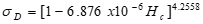
\includegraphics[width=2.07292in,height=1.375in]{media/03/image5.png}
\caption{Rx determination}
\end{figure}

For any centrifugal relief calculations associated with aircraft performance, it is sufficiently exact (g ±0.000 04 {[}m/s\textsuperscript{2}{]}) to use the average earth radius. An aircraft flying eastward contributes to centrifugal relief while a westbound aircraft diminishes it.

The International Association of Geodesy publishes the following equation (accurate to 0.005\%) to calculate (local sea level gravity including the effects of centrifugal relief for* \emph{any point fixed to the earth's surface}

\[
g_{\mathrm{lsl}} = 9.780 327 \left( 1 + 0.005 300 224 \sin^2{\phi} - 0.000\,058 \sin^2{2 \phi} \right) \left[ \frac{m}{s^2} \right]
\]

The above equation is tabulated below for quick reference.

\begin{longtable}[]{@{}lll@{}}
\toprule
\begin{minipage}[b]{0.18\columnwidth}\raggedright
\textbf{Latitude\\
(deg)}\strut
\end{minipage} & \begin{minipage}[b]{0.30\columnwidth}\raggedright
\textbf{Normal}
\(g_{\mathrm{local}}\)\strut
\end{minipage} & \begin{minipage}[b]{0.25\columnwidth}\raggedright
\strut
\end{minipage}\tabularnewline
\midrule
\endhead
\begin{minipage}[t]{0.18\columnwidth}\raggedright
\strut
\end{minipage} & \begin{minipage}[t]{0.30\columnwidth}\raggedright
\((m/s^2)\)\strut
\end{minipage} & \begin{minipage}[t]{0.25\columnwidth}\raggedright
\((ft/s^2)\)\strut
\end{minipage}\tabularnewline
\begin{minipage}[t]{0.18\columnwidth}\raggedright
\textbf{0}\strut
\end{minipage} & \begin{minipage}[t]{0.30\columnwidth}\raggedright
9.780 327\strut
\end{minipage} & \begin{minipage}[t]{0.25\columnwidth}\raggedright
32.088\strut
\end{minipage}\tabularnewline
\begin{minipage}[t]{0.18\columnwidth}\raggedright
\textbf{15}\strut
\end{minipage} & \begin{minipage}[t]{0.30\columnwidth}\raggedright
9.783 659\strut
\end{minipage} & \begin{minipage}[t]{0.25\columnwidth}\raggedright
32.098\strut
\end{minipage}\tabularnewline
\begin{minipage}[t]{0.18\columnwidth}\raggedright
\textbf{30}\strut
\end{minipage} & \begin{minipage}[t]{0.30\columnwidth}\raggedright
9.792 866\strut
\end{minipage} & \begin{minipage}[t]{0.25\columnwidth}\raggedright
32.188\strut
\end{minipage}\tabularnewline
\begin{minipage}[t]{0.18\columnwidth}\raggedright
\textbf{45}\strut
\end{minipage} & \begin{minipage}[t]{0.30\columnwidth}\raggedright
9.805 689\strut
\end{minipage} & \begin{minipage}[t]{0.25\columnwidth}\raggedright
32.171\strut
\end{minipage}\tabularnewline
\begin{minipage}[t]{0.18\columnwidth}\raggedright
\textbf{60}\strut
\end{minipage} & \begin{minipage}[t]{0.30\columnwidth}\raggedright
9.818 795\strut
\end{minipage} & \begin{minipage}[t]{0.25\columnwidth}\raggedright
32.214\strut
\end{minipage}\tabularnewline
\begin{minipage}[t]{0.18\columnwidth}\raggedright
\textbf{75}\strut
\end{minipage} & \begin{minipage}[t]{0.30\columnwidth}\raggedright
9.828 569\strut
\end{minipage} & \begin{minipage}[t]{0.25\columnwidth}\raggedright
32.249\strut
\end{minipage}\tabularnewline
\begin{minipage}[t]{0.18\columnwidth}\raggedright
\textbf{90}\strut
\end{minipage} & \begin{minipage}[t]{0.30\columnwidth}\raggedright
9.832 185\strut
\end{minipage} & \begin{minipage}[t]{0.25\columnwidth}\raggedright
32.258\strut
\end{minipage}\tabularnewline
\bottomrule
\end{longtable}

The standard acceleration (\(g_0\)) corresponds to a latitude of \(46.0625°\).

\(g_{\mathrm{lsl}}\)* at the equator and the poles varies ±0.27\% from \(g_0\).

\hypertarget{altitude-effect-on-gravitational-acceleration}{%
\subsection*{Altitude Effect on Gravitational Acceleration}\label{altitude-effect-on-gravitational-acceleration}}
\addcontentsline{toc}{subsection}{Altitude Effect on Gravitational Acceleration}

\(R_A\) is the sum of the earth's local radius and the geometric distance, \(h_G\) above the surface: \(R_A = R + h_G\)

\[
g_{\mathrm{alt}} = g_{\mathrm{lsl}}\left( \frac{R}{R + h_G} \right)^2
\]

Gravitational acceleration at any geometric altitude:

\begin{longtable}[]{@{}ll@{}}
\toprule
\begin{minipage}[b]{0.16\columnwidth}\raggedright
\(h_G\)
(1000 ft)\strut
\end{minipage} & \begin{minipage}[b]{0.26\columnwidth}\raggedright
\(g_{\mathrm{alt}}/g_{\mathrm{lsl}}\)\strut
\end{minipage}\tabularnewline
\midrule
\endhead
\begin{minipage}[t]{0.16\columnwidth}\raggedright
0\strut
\end{minipage} & \begin{minipage}[t]{0.26\columnwidth}\raggedright
1\strut
\end{minipage}\tabularnewline
\begin{minipage}[t]{0.16\columnwidth}\raggedright
10\strut
\end{minipage} & \begin{minipage}[t]{0.26\columnwidth}\raggedright
0.999 04\strut
\end{minipage}\tabularnewline
\begin{minipage}[t]{0.16\columnwidth}\raggedright
20\strut
\end{minipage} & \begin{minipage}[t]{0.26\columnwidth}\raggedright
0.998 09\strut
\end{minipage}\tabularnewline
\begin{minipage}[t]{0.16\columnwidth}\raggedright
40\strut
\end{minipage} & \begin{minipage}[t]{0.26\columnwidth}\raggedright
0.996 18\strut
\end{minipage}\tabularnewline
\begin{minipage}[t]{0.16\columnwidth}\raggedright
60\strut
\end{minipage} & \begin{minipage}[t]{0.26\columnwidth}\raggedright
0.994 28\strut
\end{minipage}\tabularnewline
\begin{minipage}[t]{0.16\columnwidth}\raggedright
80\strut
\end{minipage} & \begin{minipage}[t]{0.26\columnwidth}\raggedright
0.992 38\strut
\end{minipage}\tabularnewline
\begin{minipage}[t]{0.16\columnwidth}\raggedright
100\strut
\end{minipage} & \begin{minipage}[t]{0.26\columnwidth}\raggedright
0.990 49\strut
\end{minipage}\tabularnewline
\bottomrule
\end{longtable}

\hypertarget{actual-gravitational-pull-on-an-aircraft}{%
\subsection*{Actual Gravitational Pull on an Aircraft}\label{actual-gravitational-pull-on-an-aircraft}}
\addcontentsline{toc}{subsection}{Actual Gravitational Pull on an Aircraft}

Adding a centrifugal relief correction due to the aircraft's velocity, a complete calculation for its gravitational acceleration is
\[
g_{A/C} = \left[ g_{\mathrm{lsl}} + \omega^2 R \cos{\phi} \right] \left[ \frac{R}{R + h_G} \right]^2 - \left( \omega + \frac{V_G \sin{\sigma}}{R + h_G} \right)^2 \left(R + h_G\right) \cos{\phi}
\]

where \(V_G\) = ground speed and \(\sigma\) = ground track angle (\(0°\) = true North, \(90°\) = East, etc.).

\hypertarget{gravity-influence-on-aircraft-cruise-performance}{%
\subsection*{Gravity Influence on Aircraft Cruise Performance}\label{gravity-influence-on-aircraft-cruise-performance}}
\addcontentsline{toc}{subsection}{Gravity Influence on Aircraft Cruise Performance}

Even at the same altitude, changes in gravity due to latitude or centrifugal relief directly alter the required lift, drag, and fuel flow. For example, with sufficiently precise instrumentation, data collected heading West could show about 0.5\% more drag and fuel flow than data collected heading East (centrifugal relief effect). After determining test and standard (or mission) values for \(g\), flight test values for \(C_L\), \(C_D\), drag, and fuel flow can be corrected to standard as follows:

\[C_{L_{\mathrm{std}}} = C_{L_t} \frac{N_{z_{\omega_{\mathrm{std}}}}}{N_{Z_{\omega_t}}} \left[\frac{g_{\mathrm{std}}}{g_{A/C}} \right] \]

\[C_{D_{\mathrm{std}}} = \frac{C^2_{L_{\mathrm{std}}}}{\pi \mathrm{AR}e} \]

\[\Delta D = D_{\mathrm{std}} - D_t = qS\left[C_{D_{i_{\mathrm{std}}}} - C_{D_{i_t}} \right] \]

\[\dot{W}_{f_{\mathrm{std}}} = \dot{W}_{f_t} + \Delta D \cdot TFSC \]

where \(N_z\) = normal load factor,

\(C_L\) = lift coefficient, \(C_D\) = drag coefficient,

\(\mathrm{AR}\) = aspect ratio, \(e\) = Oswald efficiency factor,

\(\Delta D\) = change in drag force,

\(TSFC\) = thrust specific fuel consumption, and
\(\dot{W}_{f_{\mathrm{std}}}\) = standard day fuel flow

\hypertarget{general-properties-of-air}{%
\section{General Properties of Air}\label{general-properties-of-air}}

(reference 3.9.1)

\begin{longtable}[]{@{}llll@{}}
\toprule
Property & Symbol & Value & Unit\tabularnewline
\midrule
\endhead
Gas constant & \(R\) & 53.35 & ft lb/R lbm\tabularnewline
& & 287.074 & J/kg K\tabularnewline
& & 1716 & lb(ft)/slgs(R)\tabularnewline
& & 3089.7 & lb(ft)/slgs(K)\tabularnewline
Speed of sound & \(a_0 \sqrt{\theta}\) & 49.02 \(\sqrt{T_R}\) & ft/sec\tabularnewline
& & 33.42 \(\sqrt{T_R}\) & miles/hr\tabularnewline
& & 29.04 \(\sqrt{T_R}\) & knots\tabularnewline
& & 20.05 \(\sqrt{T_R}\) & m/sec\tabularnewline
Density & \(\rho\) & 0.002 3769 & slug/ft\textsuperscript{3}\tabularnewline
& & 1.225 & kg/m\textsuperscript{3} (at \(15°\)C)\tabularnewline
Specific weight & \(g_\rho\) & 0.076 47 & sec\textsuperscript{2}/ft\textsuperscript{4}\tabularnewline
Specific heat capacity at \(59°\)F (=\(T_0\)) & & &\tabularnewline
at constant pressure & \(c_p\) & 0.240 & BTU/lb R\tabularnewline
& & 1004.76 & J/kg K\tabularnewline
at constant volume & \(c_v\) & 0.1715 & BTU/lb R\tabularnewline
\bottomrule
\end{longtable}

\hypertarget{normal-composition-of-clean-dry-atmospheric-air-near-sea-level-by-volume}{%
\subsection*{Normal Composition of clean, dry atmospheric air near sea level, by volume}\label{normal-composition-of-clean-dry-atmospheric-air-near-sea-level-by-volume}}
\addcontentsline{toc}{subsection}{Normal Composition of clean, dry atmospheric air near sea level, by volume}

\begin{longtable}[]{@{}lll@{}}
\toprule
Gas & Symbol & Proportion\tabularnewline
\midrule
\endhead
Nitrogen & N\textsubscript{2} & 78.084 \%\tabularnewline
Oxygen & O\textsubscript{2} & 0.948 \%\tabularnewline
Argon & A & 0.934 \%\tabularnewline
Carbon Dioxide & CO\textsubscript{2} & 0.031 \%\tabularnewline
Neon & Ne & 0.002 \%\tabularnewline
\textbf{TOTAL} & & 99.9988 \%\tabularnewline
\bottomrule
\end{longtable}

plus traces of helium, kryton, xenon, hydrogen, methane, nitrous oxide, ozone, sulfur dioxide, nitrogen dioxide, ammonia, carbon monoxide, and iodine.

\hypertarget{viscosities-of-air}{%
\subsection*{Viscosities of Air}\label{viscosities-of-air}}
\addcontentsline{toc}{subsection}{Viscosities of Air}

Coefficient of Viscosity
\[ \mu_c = \frac{7.3025 \times 10^{-7} \left(T_R \right)^{3/2}}{T_R + 198.72} \text{ lb/ft sec}\]

Kinematic viscosity
\[ \nu = \frac{\mu_c}{g\rho} \text{ ft}^{2}\text{/sec} \]

Absolute Viscosity
\[ \mu = \rho\nu = \left[ 0.317 \left(T_R\right)^{3/2} \left( \frac{734.7}{T_R + 216} \right) \right] \times 10^{-10} \text{ lb sec/ft}^{2} \]

\hypertarget{atmospheric-viscosity-u.s.-standard-atmosphere}{%
\subsection*{Atmospheric Viscosity (U.S. Standard Atmosphere)}\label{atmospheric-viscosity-u.s.-standard-atmosphere}}
\addcontentsline{toc}{subsection}{Atmospheric Viscosity (U.S. Standard Atmosphere)}

\begin{longtable}[]{@{}lll@{}}
\toprule
\begin{minipage}[b]{0.25\columnwidth}\raggedright
Pressure Altitude

\emph{ft}\strut
\end{minipage} & \begin{minipage}[b]{0.28\columnwidth}\raggedright
Kinematic Viscosity

\emph{υ (} \emph{ft\textsuperscript{2}/sec)}\strut
\end{minipage} & \begin{minipage}[b]{0.28\columnwidth}\raggedright
Absolute Viscosity

\emph{μ~(lb sec/ft\textsuperscript{2})}\strut
\end{minipage}\tabularnewline
\midrule
\endhead
\begin{minipage}[t]{0.25\columnwidth}\raggedright
0\strut
\end{minipage} & \begin{minipage}[t]{0.28\columnwidth}\raggedright
1.572 x 10\textsuperscript{-4}\strut
\end{minipage} & \begin{minipage}[t]{0.28\columnwidth}\raggedright
3.737 x 10\textsuperscript{-7}\strut
\end{minipage}\tabularnewline
\begin{minipage}[t]{0.25\columnwidth}\raggedright
5000\strut
\end{minipage} & \begin{minipage}[t]{0.28\columnwidth}\raggedright
1.776\strut
\end{minipage} & \begin{minipage}[t]{0.28\columnwidth}\raggedright
3.638\strut
\end{minipage}\tabularnewline
\begin{minipage}[t]{0.25\columnwidth}\raggedright
10 000\strut
\end{minipage} & \begin{minipage}[t]{0.28\columnwidth}\raggedright
2.013\strut
\end{minipage} & \begin{minipage}[t]{0.28\columnwidth}\raggedright
3.538\strut
\end{minipage}\tabularnewline
\begin{minipage}[t]{0.25\columnwidth}\raggedright
15 000\strut
\end{minipage} & \begin{minipage}[t]{0.28\columnwidth}\raggedright
2.293\strut
\end{minipage} & \begin{minipage}[t]{0.28\columnwidth}\raggedright
3.435\strut
\end{minipage}\tabularnewline
\begin{minipage}[t]{0.25\columnwidth}\raggedright
20 000\strut
\end{minipage} & \begin{minipage}[t]{0.28\columnwidth}\raggedright
2.625\strut
\end{minipage} & \begin{minipage}[t]{0.28\columnwidth}\raggedright
3.330\strut
\end{minipage}\tabularnewline
\begin{minipage}[t]{0.25\columnwidth}\raggedright
25 000\strut
\end{minipage} & \begin{minipage}[t]{0.28\columnwidth}\raggedright
3.019\strut
\end{minipage} & \begin{minipage}[t]{0.28\columnwidth}\raggedright
3.224\strut
\end{minipage}\tabularnewline
\begin{minipage}[t]{0.25\columnwidth}\raggedright
30 000\strut
\end{minipage} & \begin{minipage}[t]{0.28\columnwidth}\raggedright
3.493\strut
\end{minipage} & \begin{minipage}[t]{0.28\columnwidth}\raggedright
3.115\strut
\end{minipage}\tabularnewline
\begin{minipage}[t]{0.25\columnwidth}\raggedright
35 000\strut
\end{minipage} & \begin{minipage}[t]{0.28\columnwidth}\raggedright
4.065\strut
\end{minipage} & \begin{minipage}[t]{0.28\columnwidth}\raggedright
3.004\strut
\end{minipage}\tabularnewline
\begin{minipage}[t]{0.25\columnwidth}\raggedright
40 000\strut
\end{minipage} & \begin{minipage}[t]{0.28\columnwidth}\raggedright
5.074\strut
\end{minipage} & \begin{minipage}[t]{0.28\columnwidth}\raggedright
2.981\strut
\end{minipage}\tabularnewline
\begin{minipage}[t]{0.25\columnwidth}\raggedright
45 000\strut
\end{minipage} & \begin{minipage}[t]{0.28\columnwidth}\raggedright
6.453\strut
\end{minipage} & \begin{minipage}[t]{0.28\columnwidth}\raggedright
2.982\strut
\end{minipage}\tabularnewline
\begin{minipage}[t]{0.25\columnwidth}\raggedright
50 000\strut
\end{minipage} & \begin{minipage}[t]{0.28\columnwidth}\raggedright
8.206\strut
\end{minipage} & \begin{minipage}[t]{0.28\columnwidth}\raggedright
2.983\strut
\end{minipage}\tabularnewline
\begin{minipage}[t]{0.25\columnwidth}\raggedright
55 000\strut
\end{minipage} & \begin{minipage}[t]{0.28\columnwidth}\raggedright
10.44\strut
\end{minipage} & \begin{minipage}[t]{0.28\columnwidth}\raggedright
2.985\strut
\end{minipage}\tabularnewline
\begin{minipage}[t]{0.25\columnwidth}\raggedright
60 000\strut
\end{minipage} & \begin{minipage}[t]{0.28\columnwidth}\raggedright
13.27\strut
\end{minipage} & \begin{minipage}[t]{0.28\columnwidth}\raggedright
2.986\strut
\end{minipage}\tabularnewline
\begin{minipage}[t]{0.25\columnwidth}\raggedright
70 000\strut
\end{minipage} & \begin{minipage}[t]{0.28\columnwidth}\raggedright
21.69\strut
\end{minipage} & \begin{minipage}[t]{0.28\columnwidth}\raggedright
3.005\strut
\end{minipage}\tabularnewline
\begin{minipage}[t]{0.25\columnwidth}\raggedright
80 000\strut
\end{minipage} & \begin{minipage}[t]{0.28\columnwidth}\raggedright
35.75\strut
\end{minipage} & \begin{minipage}[t]{0.28\columnwidth}\raggedright
3.043\strut
\end{minipage}\tabularnewline
\begin{minipage}[t]{0.25\columnwidth}\raggedright
90 000\strut
\end{minipage} & \begin{minipage}[t]{0.28\columnwidth}\raggedright
58.53\strut
\end{minipage} & \begin{minipage}[t]{0.28\columnwidth}\raggedright
3.080\strut
\end{minipage}\tabularnewline
\begin{minipage}[t]{0.25\columnwidth}\raggedright
100 000\strut
\end{minipage} & \begin{minipage}[t]{0.28\columnwidth}\raggedright
95.19\strut
\end{minipage} & \begin{minipage}[t]{0.28\columnwidth}\raggedright
3.118\strut
\end{minipage}\tabularnewline
\begin{minipage}[t]{0.25\columnwidth}\raggedright
150 000\strut
\end{minipage} & \begin{minipage}[t]{0.28\columnwidth}\raggedright
1066\strut
\end{minipage} & \begin{minipage}[t]{0.28\columnwidth}\raggedright
3.572\strut
\end{minipage}\tabularnewline
\begin{minipage}[t]{0.25\columnwidth}\raggedright
200 000\strut
\end{minipage} & \begin{minipage}[t]{0.28\columnwidth}\raggedright
6880\strut
\end{minipage} & \begin{minipage}[t]{0.28\columnwidth}\raggedright
3.435\strut
\end{minipage}\tabularnewline
\bottomrule
\end{longtable}

\hypertarget{psychrometric-chart-for-seal-level-barometric-pressure}{%
\subsection*{Psychrometric Chart for Seal Level Barometric Pressure}\label{psychrometric-chart-for-seal-level-barometric-pressure}}
\addcontentsline{toc}{subsection}{Psychrometric Chart for Seal Level Barometric Pressure}

\includegraphics[width=6.98681in,height=9in]{media/03/image17.jpg}

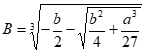
\includegraphics[width=6.98681in,height=9in]{media/03/image18.jpg}

\hypertarget{standard-atmosphere}{%
\section{Standard Atmosphere}\label{standard-atmosphere}}

\hypertarget{divisions-of-the-atmosphere}{%
\subsection*{Divisions of the Atmosphere}\label{divisions-of-the-atmosphere}}
\addcontentsline{toc}{subsection}{Divisions of the Atmosphere}

\begin{figure}
\centering
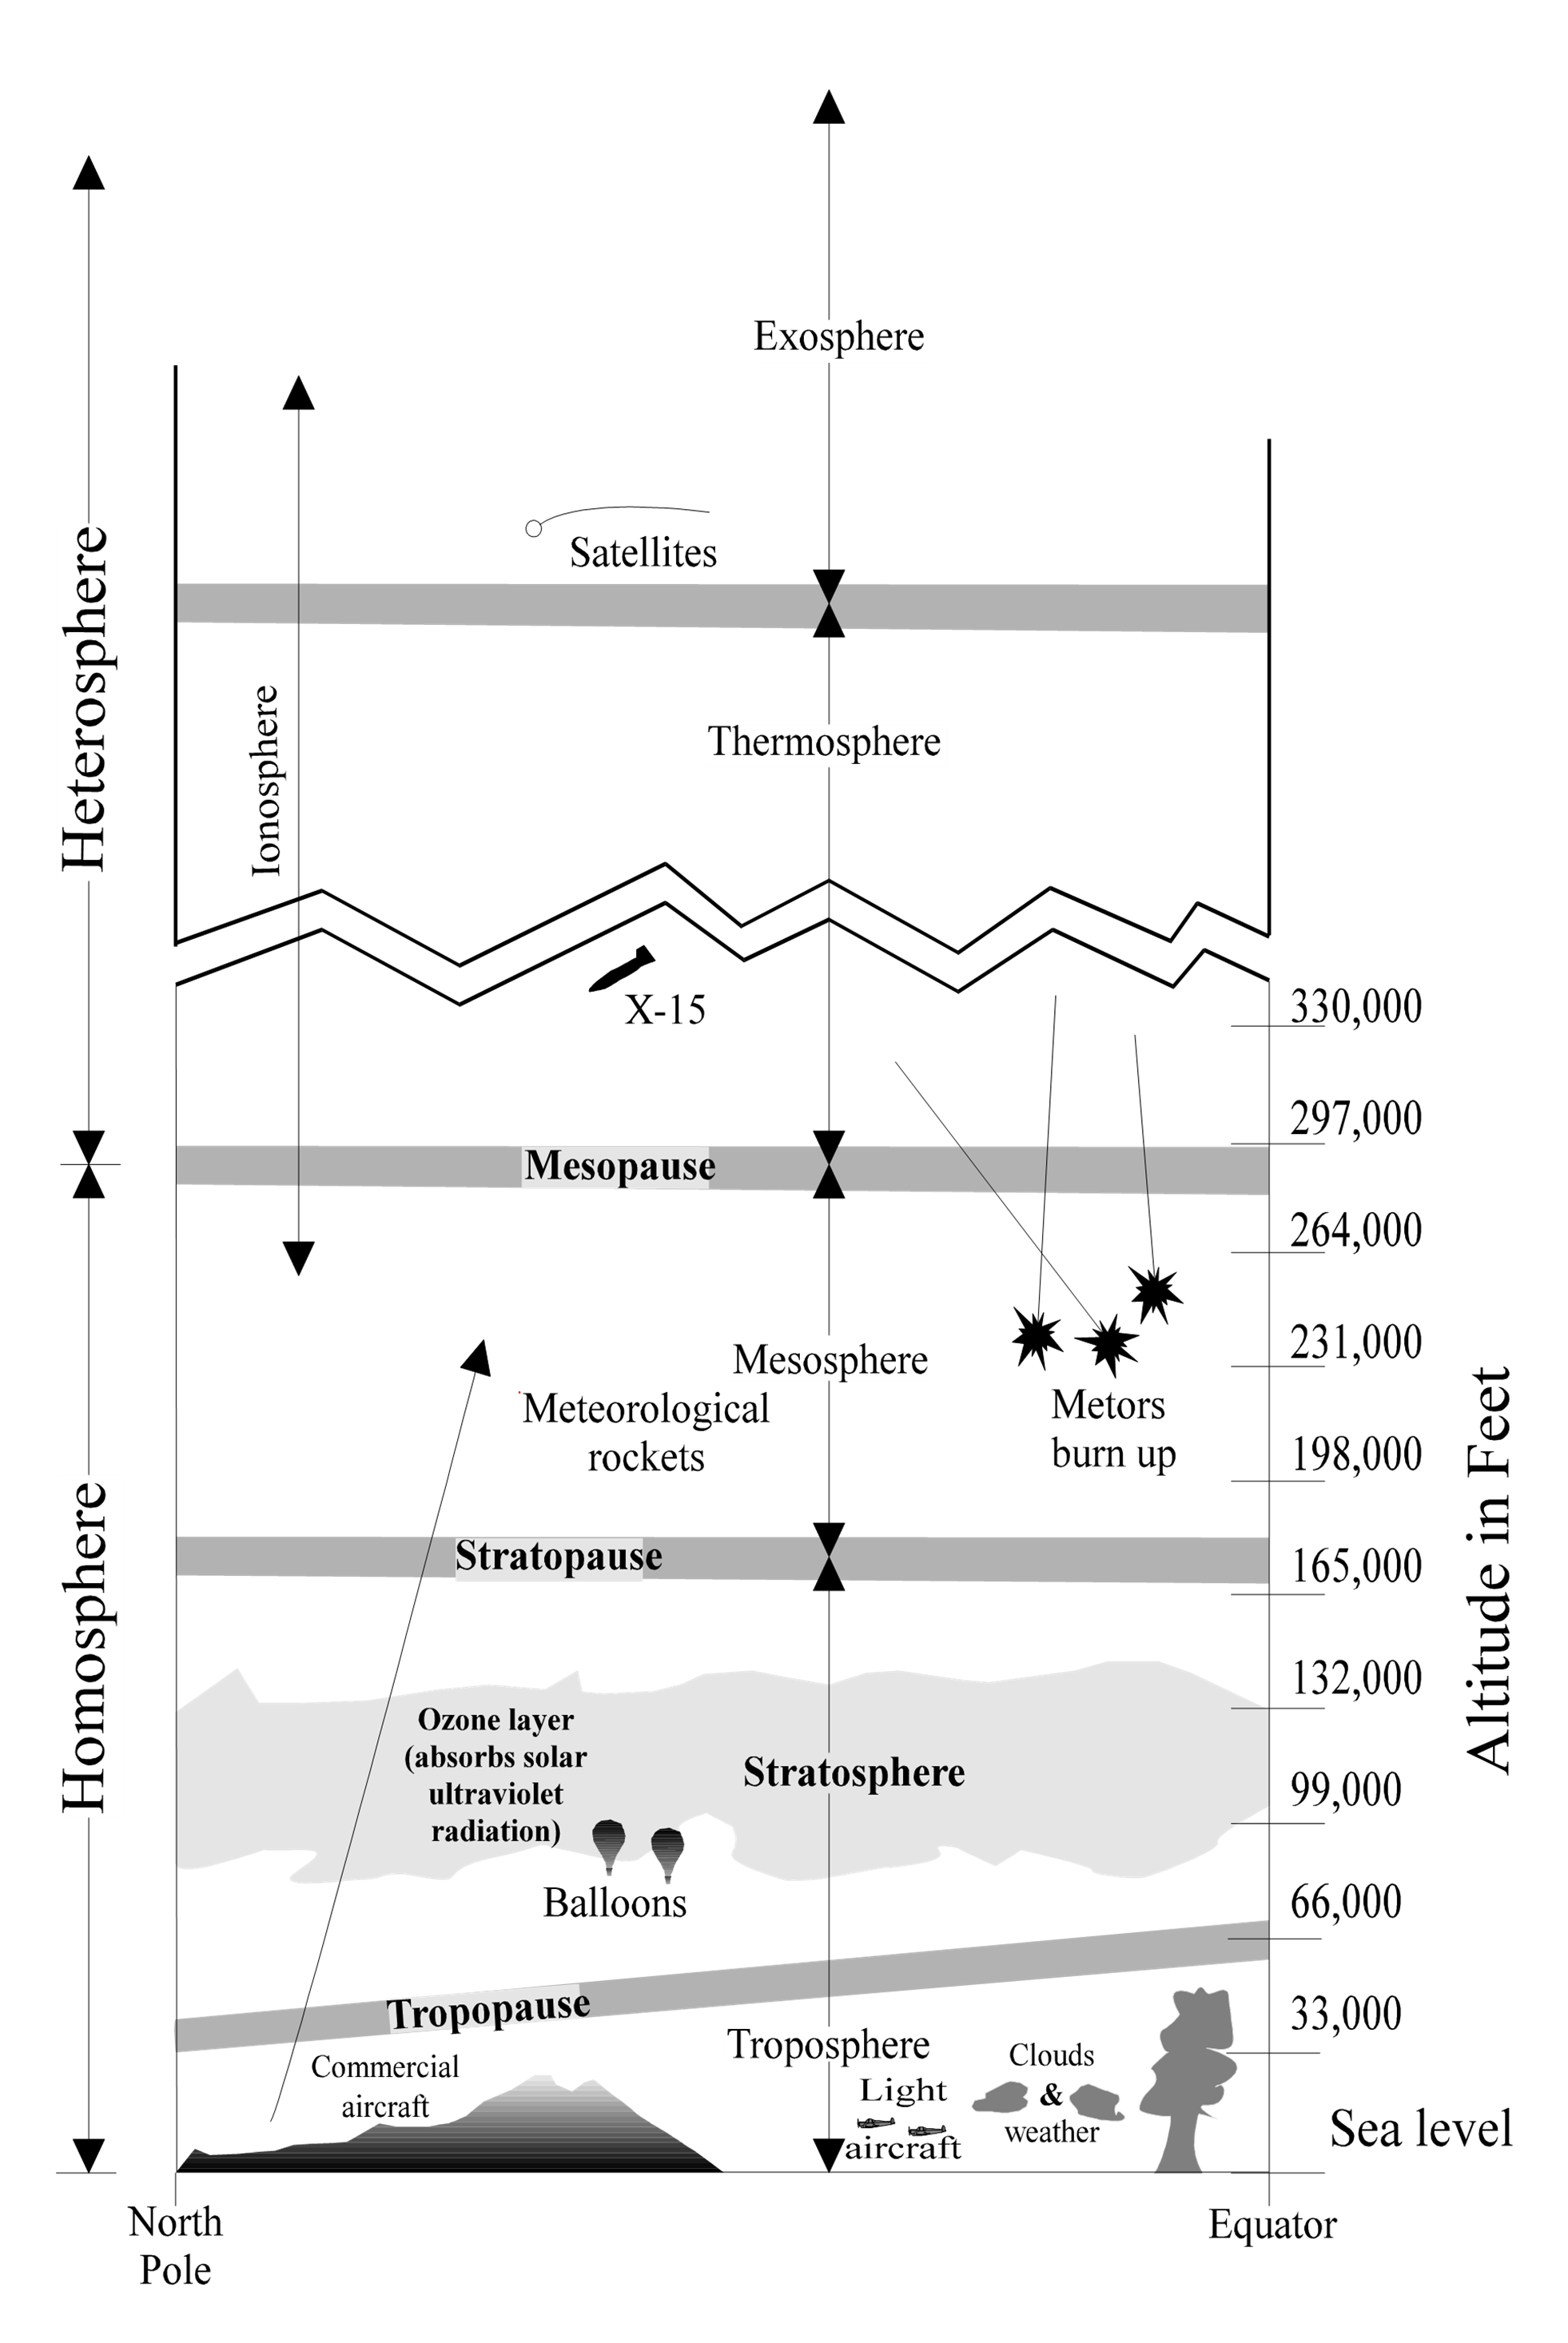
\includegraphics[width=7in,height=8.25in]{media/03/image19.png}
\caption{Divisions of the Atmosphere}
\end{figure}

Constantly changing atmospheric conditions cannot be duplicated at will to provide the exact environment in which a flight takes place. A standard atmosphere provides a common basis to relate all flight test, wind tunnel results, aircraft design and general performance. Several models of ``standard atmosphere'' exist with minor differences based on mathematical constants used in the calculations.

\begin{longtable}[]{@{}lll@{}}
\toprule
\begin{minipage}[b]{0.07\columnwidth}\raggedright
Type of Altitude\strut
\end{minipage} & \begin{minipage}[b]{0.03\columnwidth}\raggedright
Symbol\strut
\end{minipage} & \begin{minipage}[b]{0.81\columnwidth}\raggedright
Definition\strut
\end{minipage}\tabularnewline
\midrule
\endhead
\begin{minipage}[t]{0.07\columnwidth}\raggedright
Geometric\strut
\end{minipage} & \begin{minipage}[t]{0.03\columnwidth}\raggedright
\(h_G\)\strut
\end{minipage} & \begin{minipage}[t]{0.81\columnwidth}\raggedright
The height of an aircraft above sea level (also called \textbf{tapeline} altitude)\strut
\end{minipage}\tabularnewline
\begin{minipage}[t]{0.07\columnwidth}\raggedright
Absolute\strut
\end{minipage} & \begin{minipage}[t]{0.03\columnwidth}\raggedright
\(h_a\)\strut
\end{minipage} & \begin{minipage}[t]{0.81\columnwidth}\raggedright
The height of an aircraft above the center of the earth: (geometric altitude + radius of the earth)\strut
\end{minipage}\tabularnewline
\begin{minipage}[t]{0.07\columnwidth}\raggedright
Geopotential\strut
\end{minipage} & \begin{minipage}[t]{0.03\columnwidth}\raggedright
\(h\)\strut
\end{minipage} & \begin{minipage}[t]{0.81\columnwidth}\raggedright
Required because \(g\) changes with height. If potential energy is calculated using sea level weight ( \(W_{\mathrm{SL}} = mg_0\)) instead of actual weight (\(W = mg\)), then the altitude must be lower. \(h = W/W_{\mathrm{SL}} h_G\)\strut
\end{minipage}\tabularnewline
\begin{minipage}[t]{0.07\columnwidth}\raggedright
Pressure\strut
\end{minipage} & \begin{minipage}[t]{0.03\columnwidth}\raggedright
\(H_p\)\strut
\end{minipage} & \begin{minipage}[t]{0.81\columnwidth}\raggedright
The altitude, on a standard day, at which the test day pressure would be found\strut
\end{minipage}\tabularnewline
\begin{minipage}[t]{0.07\columnwidth}\raggedright
Density\strut
\end{minipage} & \begin{minipage}[t]{0.03\columnwidth}\raggedright
\(H_D\)\strut
\end{minipage} & \begin{minipage}[t]{0.81\columnwidth}\raggedright
The altitude, on a standard day, at which the test day density would be found\strut
\end{minipage}\tabularnewline
\begin{minipage}[t]{0.07\columnwidth}\raggedright
Temperature\strut
\end{minipage} & \begin{minipage}[t]{0.03\columnwidth}\raggedright
\strut
\end{minipage} & \begin{minipage}[t]{0.81\columnwidth}\raggedright
The altitude, on a standard day, at which the test day temperature would be found\strut
\end{minipage}\tabularnewline
\bottomrule
\end{longtable}

\hypertarget{assumptions-on-which-the-standard-atmosphere-is-built}{%
\subsection*{Assumptions on which the standard atmosphere is built}\label{assumptions-on-which-the-standard-atmosphere-is-built}}
\addcontentsline{toc}{subsection}{Assumptions on which the standard atmosphere is built}

\begin{enumerate}
\def\labelenumi{\arabic{enumi}.}
\tightlist
\item
  The air is dry (only 0.4\% per volume of water vapor)
\item
  The air is a perfect gas and obeys the equation of state, \(P = \rho gRT\), where \(R = 53.35 \text{ft lb/°R lbm}\)
\item
  The gravitational field decreases with altitude
\item
  Hydrostatic equilibrium exists (\(\Delta p = −\rho g_0 \Delta h\))
\end{enumerate}

\hypertarget{standard-day-sea-level-atmospheric-conditions}{%
\subsection*{Standard Day Sea Level Atmospheric Conditions}\label{standard-day-sea-level-atmospheric-conditions}}
\addcontentsline{toc}{subsection}{Standard Day Sea Level Atmospheric Conditions}

\begin{longtable}[]{@{}llll@{}}
\toprule
Parameter & Symbol & Value & Unit\tabularnewline
\midrule
\endhead
Pressure & \(P_0\) & \(2116.22\) & lb/ft\textsuperscript{2}\tabularnewline
& & \(14.696\) & lb/in\textsuperscript{2}\tabularnewline
& & \(29.921\) & in Hg\tabularnewline
& & \(1013.25\) & HPa (mb)\tabularnewline
& & \(101,325\) & Pa\tabularnewline
Temperature & \(T_0\) & \(288.15\) & K\tabularnewline
& & \(518.67\) & R\tabularnewline
& & \(59\) & °F\tabularnewline
& & \(15\) & °C\tabularnewline
Density & \(\rho_0\) & \(0.002\,3769\) & slgs/ft\textsuperscript{3}\tabularnewline
(at \(15°\)C) & & \(0.076\,47\) & lbm/in\textsuperscript{3}\tabularnewline
& & \(1.255\) & kg/m\textsuperscript{3}\tabularnewline
Speed of Sound & \(a_0\) & \(1116.45\) & ft/sec\tabularnewline
& & \(661.478\) & KTAS\tabularnewline
& & \(761.14\) & mph\tabularnewline
& & \(340.294\) & m/sec\tabularnewline
Acceleration Due to Gravity & \(g_0\) & \(32.174\) & ft/sec\textsuperscript{2}\tabularnewline
& & \(9.806,65\) & m/sec\textsuperscript{2}\tabularnewline
Temperature Lapse Rate & \(L\) & \(1.98\) & K/kft or °C/kft\tabularnewline
(up to \(36\,000\) ft or \(11\) km) & & \(3.56\) & °F/kft\tabularnewline
& & \(6.49\) & K/km\tabularnewline
\bottomrule
\end{longtable}

\hypertarget{u.s-standard-atmosphere-equations}{%
\subsection*{1976 U.S Standard Atmosphere Equations}\label{u.s-standard-atmosphere-equations}}
\addcontentsline{toc}{subsection}{1976 U.S Standard Atmosphere Equations}

\hypertarget{troposphere}{%
\subsubsection*{Troposphere}\label{troposphere}}
\addcontentsline{toc}{subsubsection}{Troposphere}

Below \(36\,089\) ft (\(11\,000\) m) and pressure less than \(22\,636\) Pa

\begin{align}
\theta &= 1 − \left( L/Τ_ο \right) h = 1 - \left( 6.875\,5856 \times 10^{-6} \right) h \\
\sigma &= \theta^{n-1} \\
\delta &= \theta^n \\
\end{align}

where \(n = 5.255\,876\), \(h\) = geopotential altitude {[}ft{]}

\hypertarget{stratosphere}{%
\subsubsection*{Stratosphere}\label{stratosphere}}
\addcontentsline{toc}{subsubsection}{Stratosphere}

Between \(36\,089\) ft and \(65\,616\) ft (\(11\,000\) m and \(20\,000\) m) the standard day temperature is a constant \(216.65\) K, therefore:

\begin{align}
\theta &= 0.751\,865 \\
\sigma &= 0.297\,076\, \mathrm{e}^{0.000\,048\,063 \left[ h - 36\,089 \right]} \\
\delta &= 0.223\,361\, \mathrm{e}^{0.000\,048\,063 \left[ h - 36\,089 \right]} \\
\end{align}

The above relations characterize the standard atmosphere table in this handbook.
They may be re-written to solve for pressure altitude (\(H_p\)) for any ambient pressure.

Below the tropopause (ambient pressure greater than \(472.683\) psf or \(22\,632\) Pa)

\[
H_p \left[ \text{ft} \right] = \frac{ 1-\left( \frac{P_a}{P_0} \right)^{0.190\,2632} }{6.875\,5856 \times 10^{-6}}
\]

In the troposphere (ambient pressure between \(114.347\) and \(472.683\) psf or between \(5475\) and \(22\,632.1\) Pascal)

\[
H_p \left[ \text{ft} \right] = 36\,089+ \frac{ \ln \left( \frac{P_a}{P_0} \right) + 1.498\,966 }{ 0.000\,048\,063 }
\]

\hypertarget{u.s.-standard-atmosphere-graph}{%
\subsubsection*{1976 U.S. Standard Atmosphere Graph}\label{u.s.-standard-atmosphere-graph}}
\addcontentsline{toc}{subsubsection}{1976 U.S. Standard Atmosphere Graph}

\begin{figure}
\centering
\includegraphics[width=5.33403in,height=5.33403in]{media/03/image22.png}
\caption{1976 US Standard Atmosphere Graph}
\end{figure}

\includegraphics[width=6.64028in,height=7.99167in]{media/03/image23.jpeg}

\includegraphics[width=6.43194in,height=9in]{media/03/image24.jpeg}

\includegraphics[width=1.98125in,height=9in]{media/03/image25.jpeg}

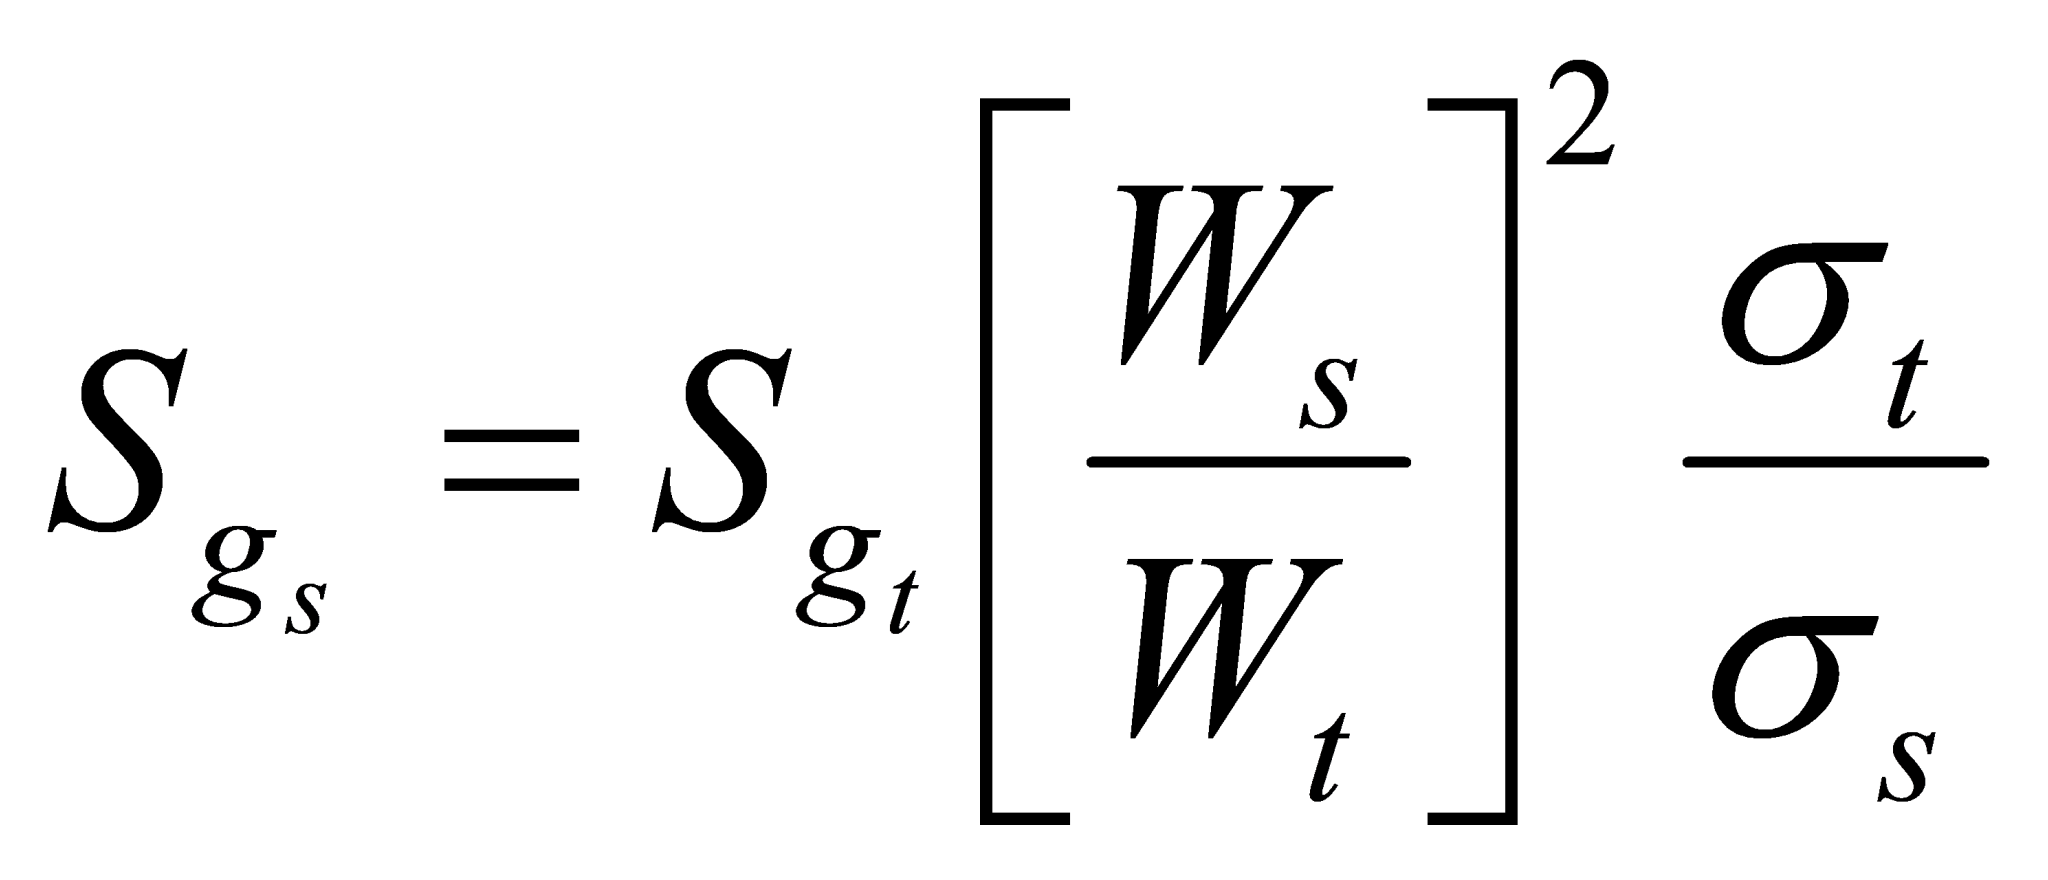
\includegraphics[width=6.99028in,height=8.99514in]{media/03/image26.jpeg}

Standard Atmosphere Calculator Website Link \url{http://www.digitaldutch.com/atmoscalc/}

\hypertarget{sea-states}{%
\section{Sea States}\label{sea-states}}

(ref 3.3)

\hypertarget{sea-scale}{%
\subsection*{Sea Scale}\label{sea-scale}}
\addcontentsline{toc}{subsection}{Sea Scale}

\begin{longtable}[]{@{}lll@{}}
\toprule
\begin{minipage}[b]{0.08\columnwidth}\raggedright
Code\strut
\end{minipage} & \begin{minipage}[b]{0.56\columnwidth}\raggedright
Sea\strut
\end{minipage} & \begin{minipage}[b]{0.27\columnwidth}\raggedright
Wave Height,

Crest to Trough {[}ft{]}\strut
\end{minipage}\tabularnewline
\midrule
\endhead
\begin{minipage}[t]{0.08\columnwidth}\raggedright
0\strut
\end{minipage} & \begin{minipage}[t]{0.56\columnwidth}\raggedright
Calm\strut
\end{minipage} & \begin{minipage}[t]{0.27\columnwidth}\raggedright
0\strut
\end{minipage}\tabularnewline
\begin{minipage}[t]{0.08\columnwidth}\raggedright
1\strut
\end{minipage} & \begin{minipage}[t]{0.56\columnwidth}\raggedright
Smooth\strut
\end{minipage} & \begin{minipage}[t]{0.27\columnwidth}\raggedright
Less than 1\strut
\end{minipage}\tabularnewline
\begin{minipage}[t]{0.08\columnwidth}\raggedright
2\strut
\end{minipage} & \begin{minipage}[t]{0.56\columnwidth}\raggedright
Slight\strut
\end{minipage} & \begin{minipage}[t]{0.27\columnwidth}\raggedright
1-3\strut
\end{minipage}\tabularnewline
\begin{minipage}[t]{0.08\columnwidth}\raggedright
3\strut
\end{minipage} & \begin{minipage}[t]{0.56\columnwidth}\raggedright
Moderate\strut
\end{minipage} & \begin{minipage}[t]{0.27\columnwidth}\raggedright
3-5\strut
\end{minipage}\tabularnewline
\begin{minipage}[t]{0.08\columnwidth}\raggedright
4\strut
\end{minipage} & \begin{minipage}[t]{0.56\columnwidth}\raggedright
Rough\strut
\end{minipage} & \begin{minipage}[t]{0.27\columnwidth}\raggedright
5-8\strut
\end{minipage}\tabularnewline
\begin{minipage}[t]{0.08\columnwidth}\raggedright
5\strut
\end{minipage} & \begin{minipage}[t]{0.56\columnwidth}\raggedright
Very rough\strut
\end{minipage} & \begin{minipage}[t]{0.27\columnwidth}\raggedright
8-12\strut
\end{minipage}\tabularnewline
\begin{minipage}[t]{0.08\columnwidth}\raggedright
6\strut
\end{minipage} & \begin{minipage}[t]{0.56\columnwidth}\raggedright
High\strut
\end{minipage} & \begin{minipage}[t]{0.27\columnwidth}\raggedright
12-20\strut
\end{minipage}\tabularnewline
\begin{minipage}[t]{0.08\columnwidth}\raggedright
7\strut
\end{minipage} & \begin{minipage}[t]{0.56\columnwidth}\raggedright
Very high\strut
\end{minipage} & \begin{minipage}[t]{0.27\columnwidth}\raggedright
20-40\strut
\end{minipage}\tabularnewline
\begin{minipage}[t]{0.08\columnwidth}\raggedright
8\strut
\end{minipage} & \begin{minipage}[t]{0.56\columnwidth}\raggedright
Mountainous\strut
\end{minipage} & \begin{minipage}[t]{0.27\columnwidth}\raggedright
40+\strut
\end{minipage}\tabularnewline
\begin{minipage}[t]{0.08\columnwidth}\raggedright
9\strut
\end{minipage} & \begin{minipage}[t]{0.56\columnwidth}\raggedright
Confused, Used as additional description 1-8\strut
\end{minipage} & \begin{minipage}[t]{0.27\columnwidth}\raggedright
\strut
\end{minipage}\tabularnewline
\bottomrule
\end{longtable}

\hypertarget{international-swell-scale}{%
\subsection*{International Swell Scale}\label{international-swell-scale}}
\addcontentsline{toc}{subsection}{International Swell Scale}

\begin{longtable}[]{@{}lll@{}}
\toprule
Code & Swell & In Open Sea\tabularnewline
\midrule
\endhead
0 & None & low\tabularnewline
1 & Short or average &\tabularnewline
2 & Long &\tabularnewline
3 & Short & Moderate height\tabularnewline
4 & Average &\tabularnewline
5 & Long &\tabularnewline
6 & Short & heavy\tabularnewline
7 & Average &\tabularnewline
8 & Long &\tabularnewline
9 & Confused, Used as additional description 1-8 &\tabularnewline
\bottomrule
\end{longtable}

\hypertarget{sunrise-sunset-times}{%
\section{Sunrise Sunset Times}\label{sunrise-sunset-times}}

\begin{figure}
\centering
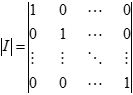
\includegraphics[width=6.99931in,height=8.74861in]{media/03/image27.png}
\caption{Sunrise Sunset Times}
\end{figure}

\hypertarget{crosswind-components}{%
\section{Crosswind Components}\label{crosswind-components}}

\begin{figure}
\centering
\includegraphics[width=6.99931in,height=6.99931in]{media/03/image28.png}
\caption{Crosswind Components}
\end{figure}

\hypertarget{geodetic-measurements}{%
\section{Geodetic Measurements}\label{geodetic-measurements}}

\hypertarget{acronyms-abbreviations-and-symbols}{%
\subsection*{Acronyms, Abbreviations and Symbols}\label{acronyms-abbreviations-and-symbols}}
\addcontentsline{toc}{subsection}{Acronyms, Abbreviations and Symbols}

\begin{longtable}[]{@{}ll@{}}
\toprule
\begin{minipage}[b]{0.43\columnwidth}\raggedright
Notation\strut
\end{minipage} & \begin{minipage}[b]{0.51\columnwidth}\raggedright
Definition\strut
\end{minipage}\tabularnewline
\midrule
\endhead
\begin{minipage}[t]{0.43\columnwidth}\raggedright
DGPS\strut
\end{minipage} & \begin{minipage}[t]{0.51\columnwidth}\raggedright
Differential Global Positioning System\strut
\end{minipage}\tabularnewline
\begin{minipage}[t]{0.43\columnwidth}\raggedright
ECEF\strut
\end{minipage} & \begin{minipage}[t]{0.51\columnwidth}\raggedright
Earth Centered Earth Fixed coordinate system\strut
\end{minipage}\tabularnewline
\begin{minipage}[t]{0.43\columnwidth}\raggedright
GPS\strut
\end{minipage} & \begin{minipage}[t]{0.51\columnwidth}\raggedright
Global Positioning System\strut
\end{minipage}\tabularnewline
\begin{minipage}[t]{0.43\columnwidth}\raggedright
INS\strut
\end{minipage} & \begin{minipage}[t]{0.51\columnwidth}\raggedright
Inertial Navigation System\strut
\end{minipage}\tabularnewline
\begin{minipage}[t]{0.43\columnwidth}\raggedright
WGS84\strut
\end{minipage} & \begin{minipage}[t]{0.51\columnwidth}\raggedright
World Geodetic System 1984\strut
\end{minipage}\tabularnewline
\begin{minipage}[t]{0.43\columnwidth}\raggedright
\(a\)\strut
\end{minipage} & \begin{minipage}[t]{0.51\columnwidth}\raggedright
Earth's semi-major axis radius\strut
\end{minipage}\tabularnewline
\begin{minipage}[t]{0.43\columnwidth}\raggedright
\(b\)\strut
\end{minipage} & \begin{minipage}[t]{0.51\columnwidth}\raggedright
Earth's semi-minor axis radius\strut
\end{minipage}\tabularnewline
\begin{minipage}[t]{0.43\columnwidth}\raggedright
\(D\)\strut
\end{minipage} & \begin{minipage}[t]{0.51\columnwidth}\raggedright
Great circle distance between two points\strut
\end{minipage}\tabularnewline
\begin{minipage}[t]{0.43\columnwidth}\raggedright
\(e\)\strut
\end{minipage} & \begin{minipage}[t]{0.51\columnwidth}\raggedright
eccentricity of the Earth square\strut
\end{minipage}\tabularnewline
\begin{minipage}[t]{0.43\columnwidth}\raggedright
\(f\)\strut
\end{minipage} & \begin{minipage}[t]{0.51\columnwidth}\raggedright
Earth's flatness factor\strut
\end{minipage}\tabularnewline
\begin{minipage}[t]{0.43\columnwidth}\raggedright
\(h\)\strut
\end{minipage} & \begin{minipage}[t]{0.51\columnwidth}\raggedright
geodetic height\strut
\end{minipage}\tabularnewline
\begin{minipage}[t]{0.43\columnwidth}\raggedright
\(N\)\strut
\end{minipage} & \begin{minipage}[t]{0.51\columnwidth}\raggedright
radius of curvature in prime vertical\strut
\end{minipage}\tabularnewline
\begin{minipage}[t]{0.43\columnwidth}\raggedright
\(P\)\strut
\end{minipage} & \begin{minipage}[t]{0.51\columnwidth}\raggedright
radius of curvature in prime vertical\strut
\end{minipage}\tabularnewline
\begin{minipage}[t]{0.43\columnwidth}\raggedright
\(\overset{\rightarrow}{P}\)\strut
\end{minipage} & \begin{minipage}[t]{0.51\columnwidth}\raggedright
Vector from earth center extending to coordinates\strut
\end{minipage}\tabularnewline
\begin{minipage}[t]{0.43\columnwidth}\raggedright
\(r\)\strut
\end{minipage} & \begin{minipage}[t]{0.51\columnwidth}\raggedright
Earth's radius\strut
\end{minipage}\tabularnewline
\begin{minipage}[t]{0.43\columnwidth}\raggedright
\(X\)\strut
\end{minipage} & \begin{minipage}[t]{0.51\columnwidth}\raggedright
ECEF x coordinate\strut
\end{minipage}\tabularnewline
\begin{minipage}[t]{0.43\columnwidth}\raggedright
\(Y\)\strut
\end{minipage} & \begin{minipage}[t]{0.51\columnwidth}\raggedright
ECEF y coordinate\strut
\end{minipage}\tabularnewline
\begin{minipage}[t]{0.43\columnwidth}\raggedright
\(Z\)\strut
\end{minipage} & \begin{minipage}[t]{0.51\columnwidth}\raggedright
ECEF z coordinate\strut
\end{minipage}\tabularnewline
\begin{minipage}[t]{0.43\columnwidth}\raggedright
\(\phi\)\strut
\end{minipage} & \begin{minipage}[t]{0.51\columnwidth}\raggedright
Geodetic latitude\strut
\end{minipage}\tabularnewline
\begin{minipage}[t]{0.43\columnwidth}\raggedright
\(\varphi\)\strut
\end{minipage} & \begin{minipage}[t]{0.51\columnwidth}\raggedright
Angle between the two \(\overset{\rightarrow}{P}\) vectors originating at the Earth's center and extending to their respective coordinates at the start and end points.\strut
\end{minipage}\tabularnewline
\begin{minipage}[t]{0.43\columnwidth}\raggedright
\(\lambda\)\strut
\end{minipage} & \begin{minipage}[t]{0.51\columnwidth}\raggedright
Geodetic longitude\strut
\end{minipage}\tabularnewline
\begin{minipage}[t]{0.43\columnwidth}\raggedright
\(\psi\)\strut
\end{minipage} & \begin{minipage}[t]{0.51\columnwidth}\raggedright
Runway heading with respect to true North.\strut
\end{minipage}\tabularnewline
\bottomrule
\end{longtable}

\hypertarget{earth-modeling}{%
\subsection*{Earth Modeling}\label{earth-modeling}}
\addcontentsline{toc}{subsection}{Earth Modeling}

The Geodetic System defines the location of any point relative to the earth using latitude, longitude and height (Figure 3.8-1, point P). Longitude and latitude are expressed in degrees, minutes, seconds. Longitude lines extend \(\pm\) 180 degrees from the Prime Meridian, run north to south, and converge at the poles. Latitude lines are parallel to the equator and extend \(\pm\) 90°.

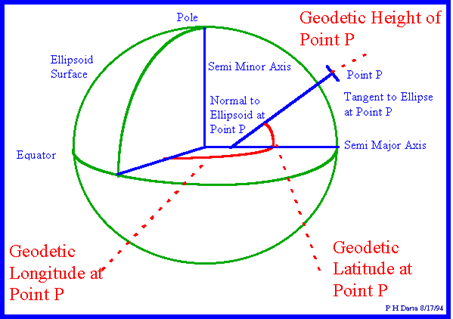
\includegraphics[width=4.71665in,height=3.32292in]{media/03/image29.png}

\texttt{http://www.colorado.edu/geography/gcraft/notes/coordsys/gif/latlon2.gif}

\textbf{Figure 3.8-1 Geodetic Coordinate System}

The 1984 world geodetic system, WGS84, models the earth's surface as an oblate spheroid - an ellipsoid rotated about its semi-minor axis. In this model, used by global positioning systems, the earth's semi-major axis, \(a\) is 6 378 137.0 meters and the semi-minor axis, \emph{b is} 6 356 752.314 meters.

The flatness factor (\(f\)) is defined as:

\[f = \frac{a - b}{a}\]

For the WGS84 model, \(f = \frac{1}{298.257\,223\,563}\)

Because the earth is not perfectly spherical, there are various methods for defining latitude. Unlike the geocentric latitude which uses the earth's center for determining a point's latitude, the \textbf{geodetic latitude} (used herein) is the angle between the equatorial plane and a line \emph{normal to the reference ellipsoid}. Figure 3.8-1 exaggerates this with a normal line being well offset from the earth's center. This definition leads to a degree of latitude being longer at the pole than at the equator: 111 694 m (60.3 nm) vs.~110 574 m (59.7 nm).

The \textbf{geodetic longitude} of a point is the angle between a reference plane and a plane passing through the point, both planes being perpendicular to the equatorial plane.

Mathematically, the geodetic surface is a smooth ellipsoid modeling the earth's surface. Clearly, the topography (actual surface height) deviates from this model whenever land is above or below sea level. Less evident is that the actual sea level also deviates from the geodetic model due to local changes in the earth's gravity. Specifically, mass variations caused by changes in earth density and topography, such as mountains or trenches, change local gravity vectors and therefore sea level relative to the ellipsoid.

Reference to \textbf{Mean Sea Level} (MSL) served as the traditional way to express topographic or bathymetric height. Geodesists once considered the sea in balance with the earth's gravity and formed a perfectly regular figure. MSL is usually described as a tidal datum that is the arithmetic mean of hourly water elevations observed over a 19-year (Metonic) cycle. This definition averages out tidal highs and lows caused by the changing effects of the gravitational forces from the moon and sun. MSL defines the zero elevation (vertical datum) for a local area. Because the sea surface conforms to the earth's gravitational field, MSL also has slight hills and valleys similar to the land surface but much smoother. Zero elevation as defined by one nation is often not the same zero elevation defined by another, thus locally defined vertical datums differ from each other.

The \textbf{Geoid} is the equipotential surface in the earth's gravity field that coincides most closely with the mean sea level extended continuously under the continents. In other words, it approximates the level of any non-flowing water connected (actually or theoretically) to the seas by waterway or via trenches or tunnels. The geoid surface undulates relative to the geodetic ellipsoid and is perpendicular to the local gravity vector -- as seen with a plumb line. Similarly, a spirit level defines the local surface parallel to the geoid, which is tangent to the local horizon. Because the geoid is an equipotential surface, it is the best datum for measuring potential energy and is the true zero surface for measuring elevations. Previously, there was no way to accurately measure the geoid, so heights were measured relative to the similar MSL. \textbf{EGM96} (Earth Gravity Model 1996) represents the best geoid model currently available and shows smoothly changing surface undulations ranging from +85 to -107 meters relative to the WGS84 ellipsoid.

The geoid surface cannot be directly observed, thus heights above or below it can't be directly measured. Instead the geoid surface is modeled mathematically using gravitational measurements. Although for practical purposes, at the coastline the geoid and MSL surfaces are assumed to be essentially the same, at some spots the geoid can actually differ from MSL by several meters.

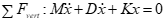
\includegraphics[width=4.69963in,height=2.63208in]{media/03/image30.jpeg}

\texttt{http://principles.ou.edu/earth\textbackslash{}\_figure\textbackslash{}\_gravity/geoid/geoid-ellipsoidal-orthometric\textbackslash{}\_height.jpg}

\textbf{Figure 3.8-2 Height Comparisons}

\textbf{Ellipsoidal height (h)} is the same as geodetic height and is the geometric distance between an object and the earth ellipsoid (Figure 3.8-2). This may be a GPS output.

\textbf{Geoid height (N)} is the height of the geoid above or below the ellipsoid. Some GPS devices output this undulation value in the data stream.

\textbf{Orthometric height (H)} is the geometric distance along a gravitational force line from a given point P to the geoid. This is essentially the conventional height measurement because the geoid approximates MSL- the traditional method for determining height.

Modern GPS units typically include a geoid model (e.g.~EGM-96) that provides N (geoid height over the WGS ellipsoid) at the current position. Such a unit can provide the height above geoid. If GPS height output is only available relative to the ellipsoid (h), then traditional Orthometric height (H) above the geoid can be obtained by subtracting the geoid height above the ellipsoid. \[http://www.esri.com/news/arcuser/0703/geoid1of3.html\]

\hypertarget{ecef-transformations}{%
\subsection*{ECEF Transformations}\label{ecef-transformations}}
\addcontentsline{toc}{subsection}{ECEF Transformations}

For the purpose of performance, navigation, or noise analysis, flight testers may require distances between two points (the shortest being along the great circle arc) and the average heading of that arc. Calculating these from typical Geodetic System Lat/Long inputs requires conversion to the Earth Centered Earth Fixed (ECEF) coordinate system as shown in Figure 3.8-3.

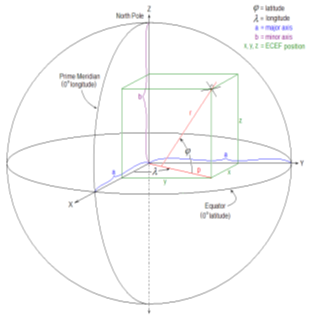
\includegraphics[width=4.37408in,height=4.46226in]{media/03/image31.png}

\textbf{Figure 3.8-3 Earth Centered Earth Fixed Coordinate System}

The ECEF coordinate system is a Cartesian system with the origin at the earth's center. In this system, the X-axis is defined by the intersection of the Prime Meridian and equatorial planes. The Z-axis goes through the North Pole. The Y-axis completes a right-handed orthogonal system by a plane 90 degrees east of the X-axis and its intersection with the equator.

Geodetic System (lat/long/height) data converts to ECEF as follows:

\begin{align}
x &= \left(N + h \right)\cos{\varphi}\cos{\lambda} \\
y &= \left(N + h \right)\cos{\varphi}\sin{\lambda} \\
z &= \left(N \left[ 1-e^2 \right] + h \right) \sin{\varphi} \\
\end{align}

where,

\(x\) = ECEF coordinate parallel to the X-axis

\(y\) = ECEF coordinate parallel to the Y-axis

\(z\) = ECEF coordinate parallel to the Z-axis

\(\varphi\) = geodetic latitude

\(\lambda\) = geodetic longitude

\(h\) = height above geodetic (ellipsoid) surface

\(N\) = Normal radius of curvature; distance from earth axis to any point on the geodetic surface at that latitude (extension of r to axis shown in Figure 3.8-3).

\[N = \frac{a}{\sqrt{ \left(1 - e^2 \right) \sin^{2}{\phi}}}\]

where,

\(a\) = semi-major axis radius (\(6\,378,137\) m; \(20\,925\,647\) ft)

\(e^2\) = eccentricity squared; \(e^{2} = 1 - \left( \frac{a}{b} \right)^{2} = 2f - f^{2}\) = 0.006 694 380 02290 (Earth, per WGS84).

Also useful is

\(M\) = Meridian radius of curvature; distance from earth axis to any point on the geodetic surface at that longitude.

\[M = \frac{a \left(1 - e^{2} \right)}{\left\lbrack \left( 1 - e^{2} \right)  \sin^{2}(\phi) \right\rbrack^{1.5}}\]

\hypertarget{great-circle-calculations}{%
\subsection*{Great Circle Calculations}\label{great-circle-calculations}}
\addcontentsline{toc}{subsection}{Great Circle Calculations}

Any plane passing through the center of a spheroid traces a \textbf{Great Circle} around the perimeter of that spheroid. The shortest distance between two points on the surface is that portion of the great circle arc encompassing both points (Figure 3.8-3).

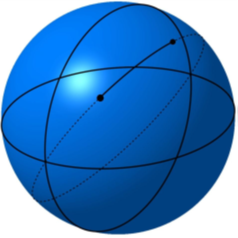
\includegraphics[width=3.30506in,height=3.31132in]{media/03/image32.png}

\textbf{Figure 3.8-3 Great Circle Arc}

Except when moving around the equator, navigating along a great circle route has the characteristic of intercepting longitude lines at different angles. In other words, the heading (or bearing) changes along the route. Analysis shows bearing \underline{change} along a great circle route:

\begin{itemize}
\tightlist
\item
  Is never greater than the longitude difference between the end points.
\item
  Approaches the value of the longitude change as the final latitude approaches a pole (regardless of initial latitude).
\item
  Is smallest when the final latitude is at the equator (for this case, bearing change ≈ longitude change x initial latitude/100).
\end{itemize}

Calculate the \textbf{great circle distance (D)} between points (subscripts 1 and 2) as

\begin{align}
P_{1} &= \sqrt{x_{1}^{2} + y_{1}^{2} + z_{1}^{2}} \\
P_{2} &= \sqrt{x_{2}^{2} + y_{2}^{2} + z_{2}^{2}} \\
\overset{\rightarrow}{P}_{1}  \overset{\rightarrow}P_{2} &= P_{1} P_{2}\cos{\varphi} = x_{1} \cdot x_{2} + y_{1} \cdot y_{2} + z_{1} \cdot z_{2} \\
\varphi &= \arccos\left( \frac{x_{1} \cdot x_{2} + y_{1} \cdot y_{2} + z_{1} \cdot z_{2}}{P_{1} \cdot P_{2}} \right) \\
D &= P_{\mathrm{avg}} \cdot \varphi
\end{align}

where
\(P\) = distance from earth center to any point (including height above the spheroid surface).

\(\overset{\rightarrow}{P}\) = Vector from the Earth's center to point P.

ϕ~= Angle between the two \(\overset{\rightarrow}{P}\) vectors

\url{http://www.movable-type.co.uk/scripts/latlong.html} provides equations an online tool for calculating great circle initial \& final bearings (headings).

For shorter distances typical of local flight testing, the Great Circle model matches the following two-dimensional approximations.

\begin{longtable}[]{@{}ll@{}}
\toprule
\endhead
Distance North-South (Northing) & \(dy = N \cdot \sin\left( \Delta\phi \right)\)\tabularnewline
Earth's radius East-West & \(r = N \cdot \cos{\phi}\)\tabularnewline
Distance East-West (Easting) & \(dx = r \cdot \sin\left(\Delta\lambda\right)\)\tabularnewline
2-D distance between two points & \(D = \sqrt{dx^2 + dy^2}\)\tabularnewline
Heading between two points (relative to true north) & \(\Phi = \arctan \left( dy/dx \right)\)\tabularnewline
\bottomrule
\end{longtable}

An error analysis of the above 2-D \textbf{heading} approximation shows it consistently lies between the initial and final headings transpiring during great circle navigation and is closest to the final heading.
This occurs when considering up to \(10\) degrees longitude change and is therefore sufficiently accurate for lesser changes that arise in flight testing (e.g.~radial from a navigation transmitter).

An error analysis of the above 2-D \textbf{distance} approximation shows accuracy within \(0.6\%\) of the great circle distance when changing latitude and longitude \(1\) degree, and within \(3\%\) when changing latitude and longitude \(10\) degrees.
It is accurate to within \(0.4\%\) when changing only latitude or longitude \(10\) degrees.

\hypertarget{local-distance-transformation}{%
\subsection*{Local Distance Transformation}\label{local-distance-transformation}}
\addcontentsline{toc}{subsection}{Local Distance Transformation}

Latitude \(\phi\), longitude \(\lambda\), and height (typical GPS output data) can be transformed into rectangular (X,Y,Z) coordinates. The following presents a method for applying this to two different coordinate systems, both with the X-Y axes defining the horizontal plane. This is useful when working with local distances associated with typical flight testing such as noise measurement, local navigation, or field performance.

Figure 3.8-4a shows a case where the X-Y coordinate system aligns with the latitude \& longitude grid. Figure 3.8-4b shows a case where the X-Y coordinate system aligns with a runway, with Y=0 defining the centerline. In both cases, a designated primary reference datum \(\phi_0, \lambda_0\), such as the runway centerline threshold, coincides with X=0, Y=0. With the example shown in Figure 3.8-4b, the opposite end of the runway centerline \(\phi_1, \lambda_1\), coincides with X = runway length and Y = 0.

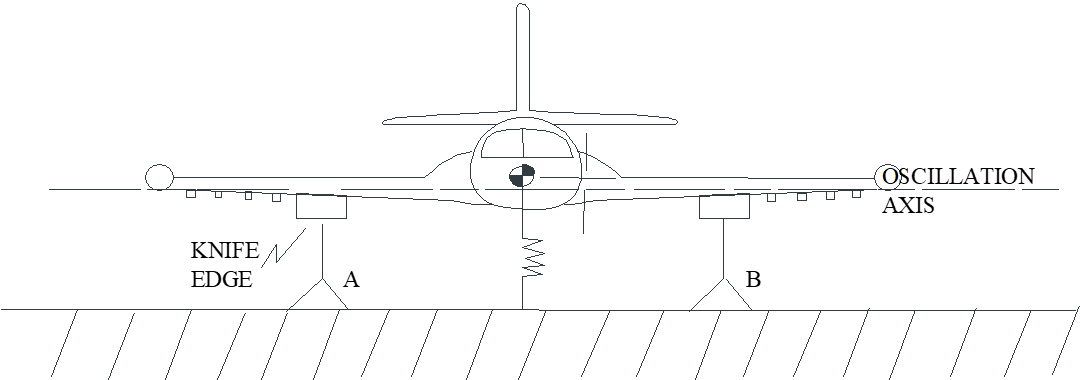
\includegraphics[width=6in,height=2.44167in]{media/03/image33.png}

\textbf{Figure 3.8-4: Local X-Y Coordinate System Aligned with (a) \(\phi\), \(\lambda\) Grid; (b) Runway}

Because each degree of latitude change is not always exactly \(60\) nm and because the spacing between degrees of longitude changes markedly with latitude, converting from degrees latitude \& longitude change to distance requires scaling factors.
First select equatorial distances for each degree change

\begin{align}
\phi_{\mathrm{scale}} \left\{ \phi = 0 \right\} &= 110\,574 \text{m} = 362\,776.6 \text{ft} = 59.705\,18 \text{nm} \\
\lambda_{\mathrm{scale}} \left\{ \phi = 0 \right\} &= 111\,319.5 \text{m} = 365\,221.4 \text{ft} = 60.107\,72 \text{nm} \\
\end{align}

Use average latitude to calculate latitude and longitude scaling factors

\begin{align}
\phi_{\mathrm{scale}} &= \frac{\phi_{\mathrm{scale}} \left\{ \phi = 0 \right\} }{ \left\lbrack \left( 1 - e^{2} \right)  \sin^{2}(\phi) \right\rbrack^{1.5} } \\
\\
\lambda_{\mathrm{scale}} &= \frac{\lbrack \lambda_{\mathrm{scale}} \left\{ \phi = 0 \right\} \rbrack \cdot \cos{\phi}}{\sqrt{ \left(1 - e^2 \right) \sin^{2}{\phi}}} \\
\end{align}

Calculate X and Y components of distances aligned with the latitude \& longitude~grid (Figure 3.8-4a)

\begin{align}
Y = \phi_{\mathrm{scale}} \left(\phi_1 - \phi_0 \right) \\
X = \lambda_{\mathrm{scale}} \left(\lambda_1 - \lambda_0 \right) \\
\end{align}

The 2-D \emph{local} (vice great circle) distance between any two points on the X-Y plane is

\[D = \sqrt{X^2 + Y^2} \]

For field performance work, it is preferable to align X \& Y with the runway as shown in Figure 3.8-4b. To convert from grid-aligned to runway-aligned coordinates, apply a rotation matrix that ensures X remains positive when going from point \(\phi_0, \lambda_0\) towards \(\phi_1, \lambda_1\). The rotation angle, \(\psi\), is positive counter-clockwise from true East to the direction of the runway. {[}Note: do not confuse \(\psi\) with runway heading measured relative to magnetic north{]}.

The function \(\psi = \mathrm{atan2} \left( X,Y \right)\) returns rotation angles from \(-\pi\) to \(\pi\), so that rotating to headings between \(90°\) and \(270°\) results in negative rotation angles.

For any point (\(\phi, \lambda\)),~calculate runway-aligned X \& Y distances using

\begin{align}
X &= \phi_{\mathrm{scale}} \left(\phi - \phi_0 \right)\sin{\psi} + \lambda_{\mathrm{scale}} \left(\lambda - \lambda_0 \right)\cos{\psi} \\
Y &= \phi_{\mathrm{scale}} \left(\phi - \phi_0 \right)\cos{\psi} - \lambda_{\mathrm{scale}} \left(\lambda - \lambda_0 \right)\sin{\psi} \\
\end{align}

This provides a right-handed rectangular coordinate system where X is positive from (\(\phi_0, \lambda_0\)) towards (\(\phi_1, \lambda_1\)) and Y is positive left of the runway centerline (Figure 3.8-4b).

Calculating aircraft height Z above the X-Y plane requires defining where the X-Y plane lies. An analyst may define Z=0 at some arbitrary height (i.e.~GPS altitude at the beginning of a maneuver) and consider only changes from that reference.

For field performance, it is typical to use the runway altitude as the reference. Because runway altitudes vary however, height should be surveyed and modeled or tabulated as a function runway centerline position, H\{X\}. For best accuracy, the runway survey accounts for GPS antenna height above the surface. Airplane height above the X-Y plane (Z) is then

\[Z = \zeta - H\{X\}\]

where \(\zeta\) is the test GPS antenna's altitude.

Note: Analysts can determine Z using either Orthometric height above the geoid (H) or above the geodetic surface (h) -- as long as the runway surface model H\{X\} uses the same reference.

\hypertarget{temperature-compensated-barometric-altitude}{%
\section{Temperature Compensated Barometric Altitude}\label{temperature-compensated-barometric-altitude}}

\textbf{Background:} Pressure altitude is the geopotential height above mean sea level (MSL) associated with atmospheric pressure on a theoretical standard day. Geopotential height is almost identical to geometric (a.k.a. tapeline) altitude, as seen in page 03-5. Altimeters set at 29.92 in Hg (or 1013 HPa) display pressure altitude. An altimeter's baro-set knob allows pilots to bias the pressure vs.~altitude relation so it matches sea level pressure for non-standard conditions. Matching the local altimeter setting (known as setting QNH in many parts of the world) adjusts the altimeter so it displays nearly the same altitude above MSL for non-standard pressure conditions. The correct setting is critical for terrain \& obstacle clearance when the pilot's visibility is low.

Note: When operating well above terrain and obstacles, it is more critical to ensure all aircraft use the same altimeter setting so they de-conflict with each other. Because chances are high that pilots might not know of or properly re-set the altimeter numerous times during high altitude flights, aviation authorities established transition altitudes. When climbing above the transition altitude, all pilots must set altimeters to read pressure altitude (baro setting at 29.92 or 10113 HPa, known as QNE or standard baro setting). Different countries use different transition altitudes (e.g.~18,000 ft MSL in U.S. and Canada; 14,000 ft MSL in Japan; 3,000 ft MSL in The Netherlands). Regardless of the transition altitude, pilots and air traffic controllers refer to altitudes above it as a ``Flight Level.'' Flight level is abbreviated as FL and is quoted in hundreds of feet above MSL. For example operating at 36,000 ft (always pressure altitude above MSL) is abbreviated as FL360.

Although the long-used practice of matching the local altimeter setting has been sufficiently safe in the vast majority of operations, it in fact does not account for temperature deviation from standard conditions. Extreme temperature deviations cause a classic mechanical altimeter to display an MSL altitude erring by hundreds of feet. Modern technology allows calculating and displaying a more accurate altitude that corrects for temperature deviations. The following equation yields temperature-compensated altitude which better estimates geometric altitude above MSL, (h\_G. Calculations require knowledge of aircraft's baro and pressure altitudes and the terminal airport's temperature and pressure altitude. In lieu of pressure altitudes, calculations allow for implementing the field elevation (depicted on airport approach plates, etc.) and so-called baro bias. Baro bias is the displayed altitude shift when switching from local to standard altimeter setting.

\[h_G = H_b + \frac{T_{\mathrm{apt}} - T_0}{L - Hp_{\mathrm{apt}} } \ln \left[ 1 + \frac{L \left( H_p - H_{p_{\mathrm{apt}}} \right) }{T_0 + L H_{p_{\mathrm{apt}}}} \right]\]

where
\(h_G\) = temperature-compensated altitude

\(H_b\) = baro altitude (displayed when altimeter is set to local value)

\(T_{\mathrm{apt}}\) = airport temperature (Kelvin)

\(T_0\) = standard day sea level temperature = 15 deg C = 288.15 K

\(L\) = standard temperature lapse rate = -0.0065 K/m = -0.001 9812 K/ft

\(H_{p_{\mathrm{apt}}}\) = airport pressure altitude ( = airport field elevation - baro bias)

\(H_p\) = aircraft pressure altitude ( = H\_b - baro bias)

Note: ensure altitude units are consistent with lapse rate units.

In lieu of the pilot adjusting the baro set knob to determine baro bias, it may be calculated using

Baro bias = \(H_b - H_p = H_b - \frac{29.92^{0.1903} - PA^{0.1903}}{0.000\,013\,13}\) {[}ft{]}

where

PA = ambient pressure = \{altimeter setting {[}in Hg{]}\textsuperscript{0.1903} - \(H_b\)(0.000 013 13)\}\textsuperscript{1/0.1903}

Flight testers can use the above to verify the aircraft's temperature compensation system is working correctly. Data analysts can use these equations to more precisely determine geometric height above the ground--potentially useful for performance or pitot-static flyby testing.

\hypertarget{references-2}{%
\section{References}\label{references-2}}

\begin{longtable}[]{@{}ll@{}}
\toprule
\endhead
\begin{minipage}[t]{0.06\columnwidth}\raggedright
3.1\strut
\end{minipage} & \begin{minipage}[t]{0.88\columnwidth}\raggedright
Anon., ``Aeronautical Vestpocket Handbook'' ,Part No.~P\&W 079500, United Technologies Pratt \& Whitney, Canada, 1990.\strut
\end{minipage}\tabularnewline
\begin{minipage}[t]{0.06\columnwidth}\raggedright
3.2\strut
\end{minipage} & \begin{minipage}[t]{0.88\columnwidth}\raggedright
Lawless, Alan. R. et al, ``Aerodynamics for Flight Testers,'' National Test Pilot School, P.O. Box 658, Mojave CA, 93501, 1999.\strut
\end{minipage}\tabularnewline
\begin{minipage}[t]{0.06\columnwidth}\raggedright
3.3\strut
\end{minipage} & \begin{minipage}[t]{0.88\columnwidth}\raggedright
Denno, Richard R., et al ``AIAA Aerospace Design Engineers Guide'' ISBN 0-930403-21-5, AIAA, 1987.\strut
\end{minipage}\tabularnewline
\begin{minipage}[t]{0.06\columnwidth}\raggedright
3.4\strut
\end{minipage} & \begin{minipage}[t]{0.88\columnwidth}\raggedright
Global Positioning System Overview, Peter H. Dana, Department of Geography, University of Texas at Austin, 1994. {[}\url{www.colorado.edu/geography/gcraft/notes/gps/gps_f.html}{]}\strut
\end{minipage}\tabularnewline
\begin{minipage}[t]{0.06\columnwidth}\raggedright
3.5\strut
\end{minipage} & \begin{minipage}[t]{0.88\columnwidth}\raggedright
Charles D Ghilani, Penn State College of Engineering, 2008 {[}\url{http://surveying.wb.psu.edu/sur351/georef/Ellip4.htm}{]} {[}\url{www.colorado.edu/geography/gcraft/notes/gps/gps_f.html}{]}\strut
\end{minipage}\tabularnewline
\begin{minipage}[t]{0.06\columnwidth}\raggedright
3.6\strut
\end{minipage} & \begin{minipage}[t]{0.88\columnwidth}\raggedright
Standard Atmosphere Calculator Website Link {[}\url{http://www.digitaldutch.com/atmoscalc/}{]}.\strut
\end{minipage}\tabularnewline
\begin{minipage}[t]{0.06\columnwidth}\raggedright
3.7\strut
\end{minipage} & \begin{minipage}[t]{0.88\columnwidth}\raggedright
Movable Type Scripts. {[}\url{http://www.movable-type.co.uk/scripts/latlong.html}{]}. {[}Calculate distance, bearing and more between Latitude/Longitude points{]}\strut
\end{minipage}\tabularnewline
\bottomrule
\end{longtable}

\hypertarget{pitot-statics}{%
\chapter{Pitot Statics}\label{pitot-statics}}

\emph{Editor's Note}

\emph{In an effort to reduce confusion and conflict regarding pitot and static pressure nomenclature, SFTE has elected to change two definitions and symbols since the first edition of this handbook was released. Henceforth, \(\Delta Ps\) shall indicate static pressure ERROR (\(\Delta P_s = P_s - P_a)\) and \(\Delta P_T\) shall indicate total (i.e.~pitot) pressure ERROR (\(\Delta P_T = P_p - P_T\)). This nomenclature eliminates the \(\Delta P_p\) symbol and confusion as to whether it indicates position error or pitot error.}

\hypertarget{common-nomenclature}{%
\section*{Common Nomenclature}\label{common-nomenclature}}
\addcontentsline{toc}{section}{Common Nomenclature}

\begin{longtable}[]{@{}ll@{}}
\toprule
\begin{minipage}[b]{0.22\columnwidth}\raggedright
Symbol\strut
\end{minipage} & \begin{minipage}[b]{0.72\columnwidth}\raggedright
Definition\strut
\end{minipage}\tabularnewline
\midrule
\endhead
\begin{minipage}[t]{0.22\columnwidth}\raggedright
\(a\)\strut
\end{minipage} & \begin{minipage}[t]{0.72\columnwidth}\raggedright
speed of sound\strut
\end{minipage}\tabularnewline
\begin{minipage}[t]{0.22\columnwidth}\raggedright
\(a_0\)\strut
\end{minipage} & \begin{minipage}[t]{0.72\columnwidth}\raggedright
speed of sound at sea level on a standard day\strut
\end{minipage}\tabularnewline
\begin{minipage}[t]{0.22\columnwidth}\raggedright
\(M\)\strut
\end{minipage} & \begin{minipage}[t]{0.72\columnwidth}\raggedright
Mach number\strut
\end{minipage}\tabularnewline
\begin{minipage}[t]{0.22\columnwidth}\raggedright
\(P_a\)\strut
\end{minipage} & \begin{minipage}[t]{0.72\columnwidth}\raggedright
ambient pressure\strut
\end{minipage}\tabularnewline
\begin{minipage}[t]{0.22\columnwidth}\raggedright
\(P_0\)\strut
\end{minipage} & \begin{minipage}[t]{0.72\columnwidth}\raggedright
ambient pressure at sea level on a standard day (\(=2116.2 lb/ft^2 = 29.92 in Hg\))\strut
\end{minipage}\tabularnewline
\begin{minipage}[t]{0.22\columnwidth}\raggedright
\(P_p\)\strut
\end{minipage} & \begin{minipage}[t]{0.72\columnwidth}\raggedright
pitot pressure corrected for instrument error only\strut
\end{minipage}\tabularnewline
\begin{minipage}[t]{0.22\columnwidth}\raggedright
\(P_s\)\strut
\end{minipage} & \begin{minipage}[t]{0.72\columnwidth}\raggedright
static pressure (indicated at static port)\strut
\end{minipage}\tabularnewline
\begin{minipage}[t]{0.22\columnwidth}\raggedright
\(P_T\)\strut
\end{minipage} & \begin{minipage}[t]{0.72\columnwidth}\raggedright
total pressure\strut
\end{minipage}\tabularnewline
\begin{minipage}[t]{0.22\columnwidth}\raggedright
\(q\)\strut
\end{minipage} & \begin{minipage}[t]{0.72\columnwidth}\raggedright
incompressible dynamic pressure\strut
\end{minipage}\tabularnewline
\begin{minipage}[t]{0.22\columnwidth}\raggedright
\(q_c\)\strut
\end{minipage} & \begin{minipage}[t]{0.72\columnwidth}\raggedright
compressible dynamic pressure (\(=P_T-P_a\))\strut
\end{minipage}\tabularnewline
\begin{minipage}[t]{0.22\columnwidth}\raggedright
\(q_{\mathrm{cic}}\)\strut
\end{minipage} & \begin{minipage}[t]{0.72\columnwidth}\raggedright
instrument corrected differential pressure (\(=P_p-P_s\))\strut
\end{minipage}\tabularnewline
\begin{minipage}[t]{0.22\columnwidth}\raggedright
\(T_a\)\strut
\end{minipage} & \begin{minipage}[t]{0.72\columnwidth}\raggedright
ambient temperature (absolute scale)\strut
\end{minipage}\tabularnewline
\begin{minipage}[t]{0.22\columnwidth}\raggedright
\(T_0\)\strut
\end{minipage} & \begin{minipage}[t]{0.72\columnwidth}\raggedright
ambient temperature at sea level on a standard day (\(=288.15 K = 15° C = 518.7°R=59.0°F\))\strut
\end{minipage}\tabularnewline
\begin{minipage}[t]{0.22\columnwidth}\raggedright
\(T_T\)\strut
\end{minipage} & \begin{minipage}[t]{0.72\columnwidth}\raggedright
total temperature (absolute scale)\strut
\end{minipage}\tabularnewline
\begin{minipage}[t]{0.22\columnwidth}\raggedright
\(V_c\)\strut
\end{minipage} & \begin{minipage}[t]{0.72\columnwidth}\raggedright
calibrated airspeed\strut
\end{minipage}\tabularnewline
\begin{minipage}[t]{0.22\columnwidth}\raggedright
\(V_e\)\strut
\end{minipage} & \begin{minipage}[t]{0.72\columnwidth}\raggedright
equivalent airspeed\strut
\end{minipage}\tabularnewline
\begin{minipage}[t]{0.22\columnwidth}\raggedright
\(V_g\)\strut
\end{minipage} & \begin{minipage}[t]{0.72\columnwidth}\raggedright
ground speed\strut
\end{minipage}\tabularnewline
\begin{minipage}[t]{0.22\columnwidth}\raggedright
\(V_i\)\strut
\end{minipage} & \begin{minipage}[t]{0.72\columnwidth}\raggedright
indicated airspeed\strut
\end{minipage}\tabularnewline
\begin{minipage}[t]{0.22\columnwidth}\raggedright
\(V_T\)\strut
\end{minipage} & \begin{minipage}[t]{0.72\columnwidth}\raggedright
true airspeed\strut
\end{minipage}\tabularnewline
\begin{minipage}[t]{0.22\columnwidth}\raggedright
\(\Delta H_{\mathrm{ic}}\)\strut
\end{minipage} & \begin{minipage}[t]{0.72\columnwidth}\raggedright
altimeter instrument correction\strut
\end{minipage}\tabularnewline
\begin{minipage}[t]{0.22\columnwidth}\raggedright
\(\Delta H_{\mathrm{pc}}\)\strut
\end{minipage} & \begin{minipage}[t]{0.72\columnwidth}\raggedright
altimeter position error correction\strut
\end{minipage}\tabularnewline
\begin{minipage}[t]{0.22\columnwidth}\raggedright
\(\Delta P_D\)\strut
\end{minipage} & \begin{minipage}[t]{0.72\columnwidth}\raggedright
dynamic pressure error (\(=P_T-\Delta P_s\))\strut
\end{minipage}\tabularnewline
\begin{minipage}[t]{0.22\columnwidth}\raggedright
\(\Delta P_T\)\strut
\end{minipage} & \begin{minipage}[t]{0.72\columnwidth}\raggedright
total (pitot) pressure error (\(=P_P-P_T\))\strut
\end{minipage}\tabularnewline
\begin{minipage}[t]{0.22\columnwidth}\raggedright
\(\Delta P_s\)\strut
\end{minipage} & \begin{minipage}[t]{0.72\columnwidth}\raggedright
static pressure error (\(=P_s-P_a\))\strut
\end{minipage}\tabularnewline
\begin{minipage}[t]{0.22\columnwidth}\raggedright
\(\Delta V_{\mathrm{ic}}\)\strut
\end{minipage} & \begin{minipage}[t]{0.72\columnwidth}\raggedright
airspeed instrument correction\strut
\end{minipage}\tabularnewline
\begin{minipage}[t]{0.22\columnwidth}\raggedright
\(\Delta V_{\mathrm{pc}}\)\strut
\end{minipage} & \begin{minipage}[t]{0.72\columnwidth}\raggedright
airspeed position error correction\strut
\end{minipage}\tabularnewline
\begin{minipage}[t]{0.22\columnwidth}\raggedright
\(\delta\)\strut
\end{minipage} & \begin{minipage}[t]{0.72\columnwidth}\raggedright
pressure ratio between ambient and sea level std (\(=P_a/P_0\))\strut
\end{minipage}\tabularnewline
\begin{minipage}[t]{0.22\columnwidth}\raggedright
\(\theta\)\strut
\end{minipage} & \begin{minipage}[t]{0.72\columnwidth}\raggedright
temperature ratio between ambient and sea level std (\(=T_a/T_0\))\strut
\end{minipage}\tabularnewline
\begin{minipage}[t]{0.22\columnwidth}\raggedright
\(\rho_0\)\strut
\end{minipage} & \begin{minipage}[t]{0.72\columnwidth}\raggedright
ambient density at sea level on a std day (\(=0.002 377 slg/ft^3\))\strut
\end{minipage}\tabularnewline
\begin{minipage}[t]{0.22\columnwidth}\raggedright
\(\sigma\)\strut
\end{minipage} & \begin{minipage}[t]{0.72\columnwidth}\raggedright
density ratio between ambient and sea level std (\(=P_a/P_0\))\strut
\end{minipage}\tabularnewline
\begin{minipage}[t]{0.22\columnwidth}\raggedright
\(\gamma\)\strut
\end{minipage} & \begin{minipage}[t]{0.72\columnwidth}\raggedright
ratio of specific heats (\(=1.4\) for air)\strut
\end{minipage}\tabularnewline
\bottomrule
\end{longtable}

\hypertarget{subsonic-airspeed-and-mach-equation}{%
\section{Subsonic Airspeed and Mach Equation}\label{subsonic-airspeed-and-mach-equation}}

True Airspeed

\[V_{T} = \left\lbrack \frac{2\gamma}{\gamma-1} \frac{P_a}{\rho_a} \left( \left\lbrack \frac{P_T - P_a}{P_a} + 1 \right\rbrack^\frac{\gamma-1}{\gamma} - 1 \right) \right\rbrack ^{1/2}\]

Equivalent Airspeed

(= \(V_T\) equation with assumption of std day sea level density)

\[V_{e} = \sqrt{7\frac{P_{a}}{\rho_0}\left( \left\lbrack \frac{P_{T} - P_{a}}{P_{a}} + 1 \right\rbrack^{\frac{2}{7}} - 1 \right)} = V_{T}\sqrt{\frac{\rho_{a}}{\rho_0}} = V_{T}\sqrt{\sigma}\]

Calibrated Airspeed

(= \(V_e\) equation with assumption of std day sea level pressure)

\[V_{c} = \left\lbrack \frac{2\gamma}{\gamma - 1}\frac{P_0}{\rho_0}\left( \left\lbrack \frac{P_{T} - P_{a}}{P_0} + 1 \right\rbrack^{\frac{\gamma - 1}{\gamma}} - 1 \right) \right\rbrack^{\frac{1}{2}}\]

\[\sqrt{7 \frac{P_0}{\rho_0}\left( \left\lbrack \frac{q_c}{P_0} + 1 \right\rbrack^{\frac{2}{7}} - 1 \right)}\]

Applying British units (\(lb/ft^2\)) and converting from \emph{ft/sec} to knots yields

\[ V_{c} = 1479\sqrt{\left\lbrack \frac{P_{T} - P_{a}}{2116} + 1 \right\rbrack^{\frac{2}{7}} - 1} ~(kts)\]

Mach Number

\[M = \frac{V_{T}}{a} = \sqrt{\frac{2}{\gamma - 1}\left\lbrack \left( \frac{P_{T} - P_{a}}{P_{a}} + 1 \right)^{\frac{\gamma - 1}{\gamma}} - 1 \right\rbrack} = \sqrt{5\left( \left\lbrack \frac{q_{c}}{P_{a}} + 1 \right\rbrack^{\frac{2}{7}} - 1 \right)}\]

\hypertarget{scale-altitude-compressibility-correction}{%
\section{Scale Altitude (Compressibility ) Correction}\label{scale-altitude-compressibility-correction}}

The name comes from the fact that although the equivalent airspeed equation does correct for compressibility, the sea level pressure assumption used for calibrated airspeed makes the compressibility correction valid only for that (sea level) pressure. Above sea level, the calibrated airspeed must be re-scaled for pressure effects on compressibility. The mathematical method for determining \(V_e\) from \(V_c\) is to first solve the calibrated airspeed equation for \(q_c\).

\[q_c = P_0  \left\lbrack \left( \frac{\rho_0}{P_0} \frac{V_c^2}{7} + 1 \right)^{3.5} - 1 \right\rbrack\]

Next, substitute this value and the ambient pressure (\(P_a\)) into the equivalent airspeed equation. (\(q_c = P_T - P_a\))

\[V_e = \sqrt{7 \frac{P_a}{\rho_0} \left( \left\lbrack \frac{q_c}{P_a}+1 \right\rbrack^{2/7} - 1 \right) } \]

The adjacent chart does this graphically for all subsonic airspeeds.

\[V_e = V_c + \Delta V_c\]

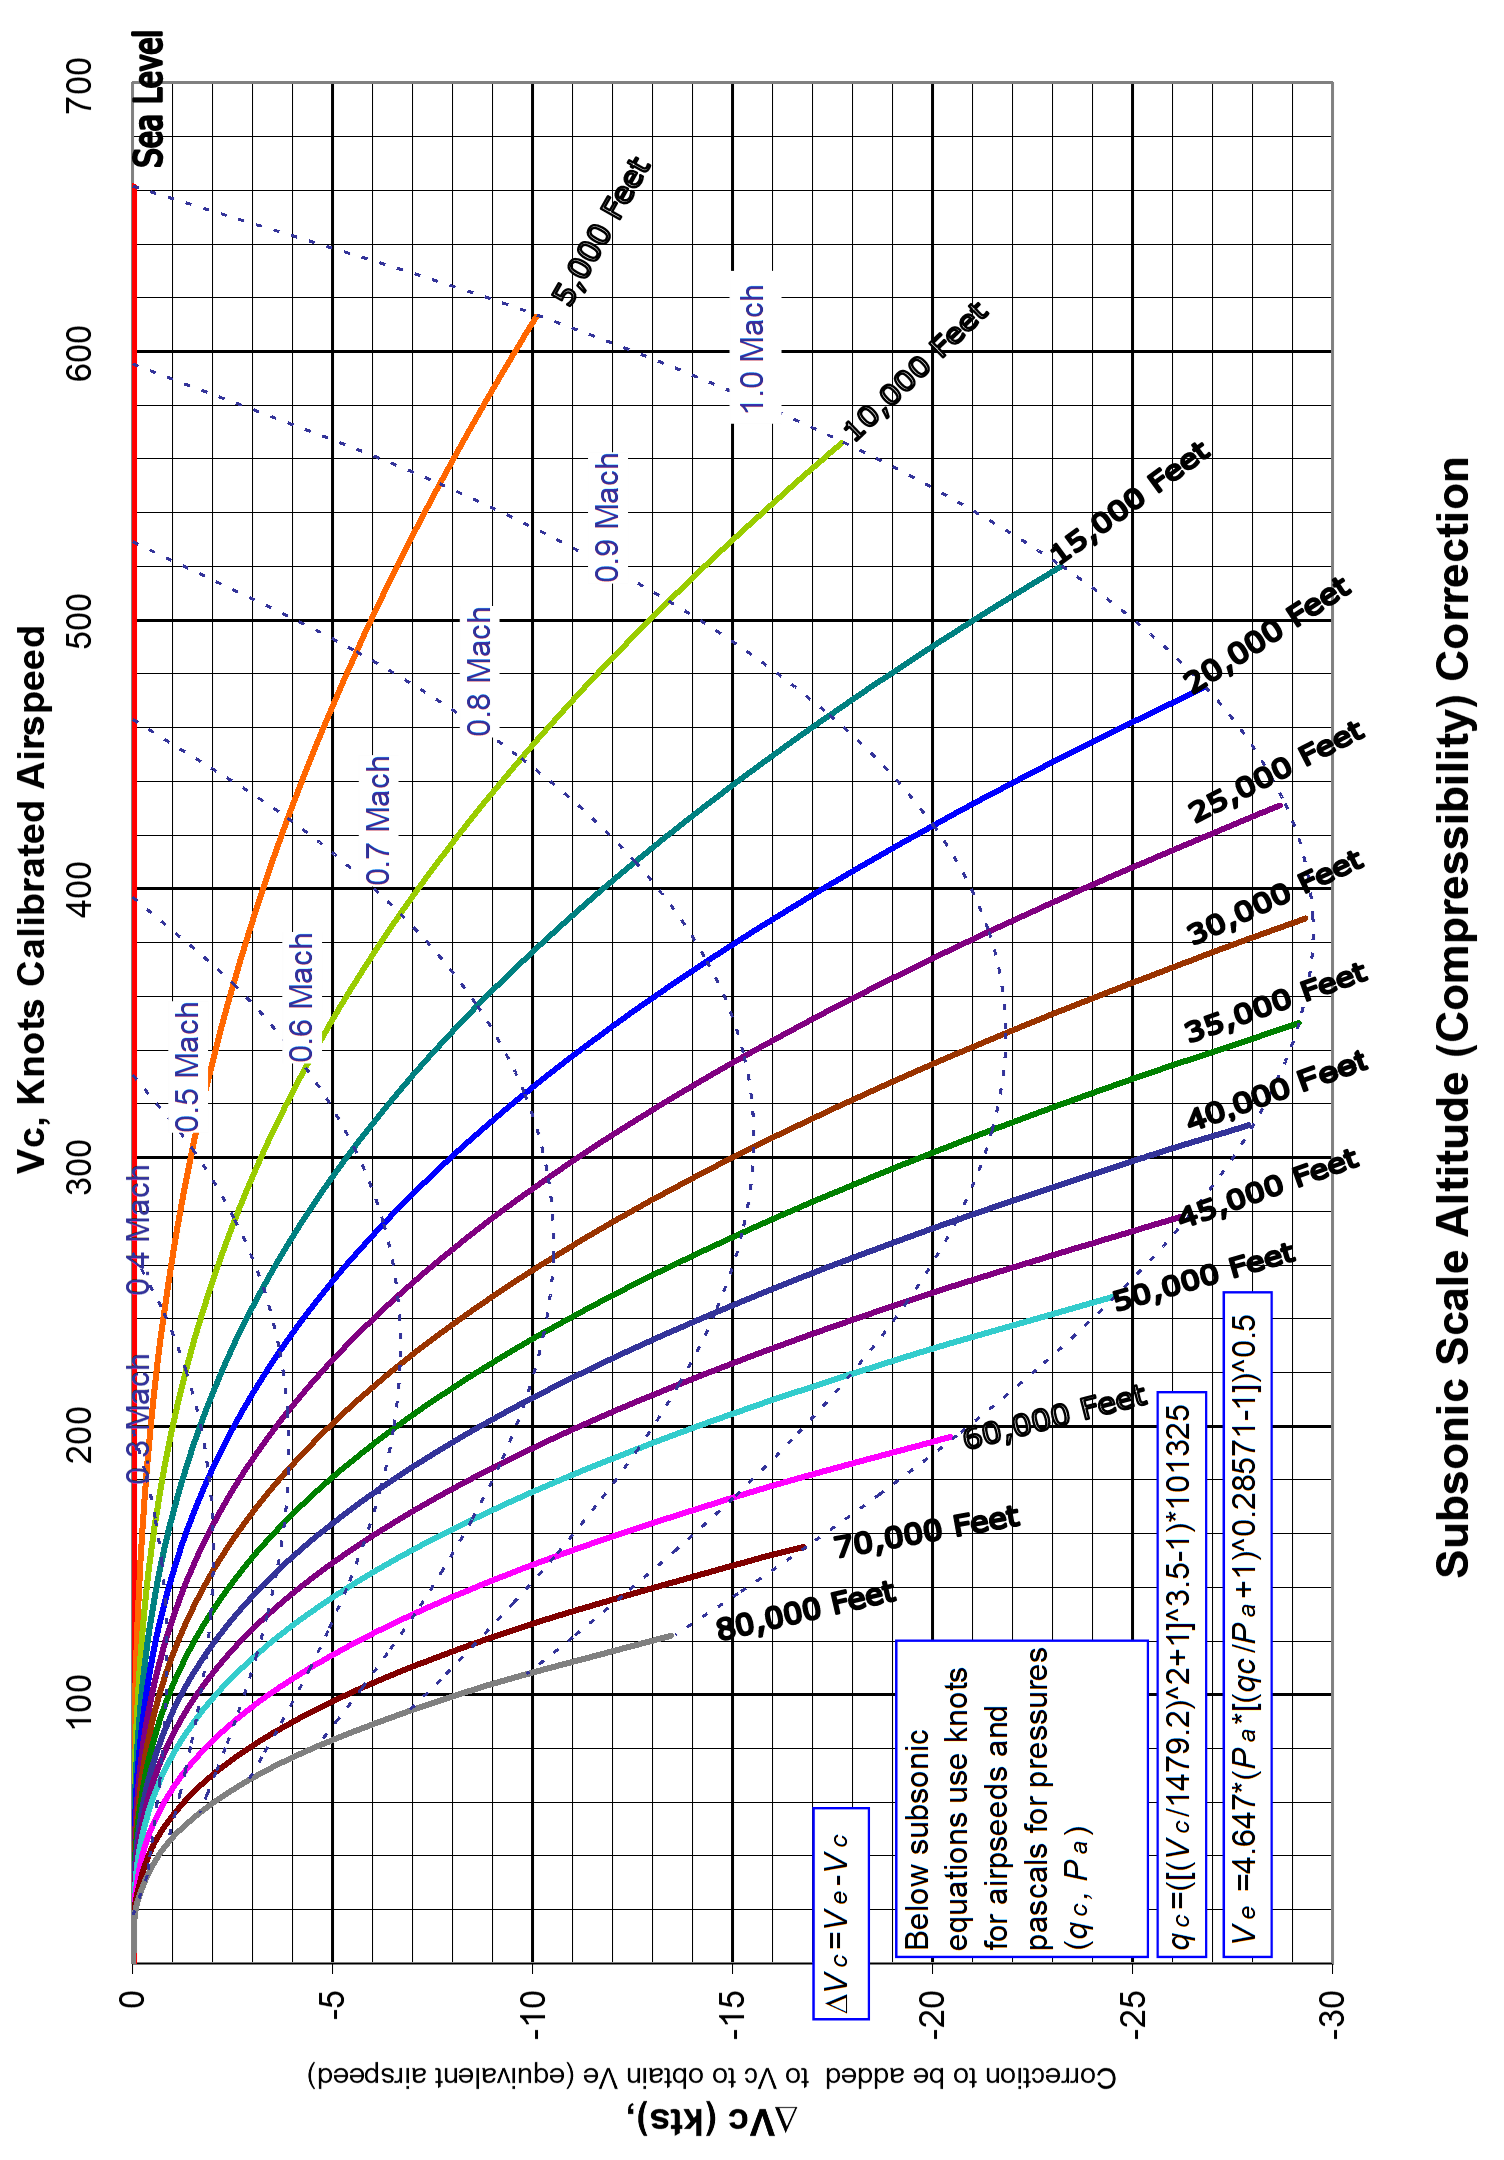
\includegraphics[width=6.20764in,height=8.91528in]{media/04/image3.png}

\hypertarget{subsonic-relations-between-compressible-and-incompressible-dynamic-pressure}{%
\section{Subsonic Relations Between Compressible and Incompressible Dynamic Pressure}\label{subsonic-relations-between-compressible-and-incompressible-dynamic-pressure}}

For constant density (incompressible) flow Bernoulli's equation reduces to

\[V_T = \sqrt{\frac{2}{\rho_a}(P_T - P_a)} = \sqrt{\frac{2q}{\rho_a}} \]

Where incompressible dynamic pressure \(q\) is defined as \(P_T-P_a\).

As airflow speed increases, its density at the stagnation point increases thereby increasing the sensed pressure. The ratio between compressible \& incompressible dynamic pressure can be written as a function of Mach number

\[q_c = q \left\lbrack 1 + \frac{M^2}{4} + \frac{M^4}{40} + \frac{M^6}{1600} + ... \right\rbrack \]

True dynamic pressure \(q\) (as used in modeling) is defined in dimensional analysis as:

\[q = \frac{1}{2} \rho_a V_T^2 = \frac{1}{2}\rho_0V_e^2\]

This value for \(q\) should not be confused with compressible (a.k.a. impact or differential) pressure, \(q_c (= P_T - P_a)\)

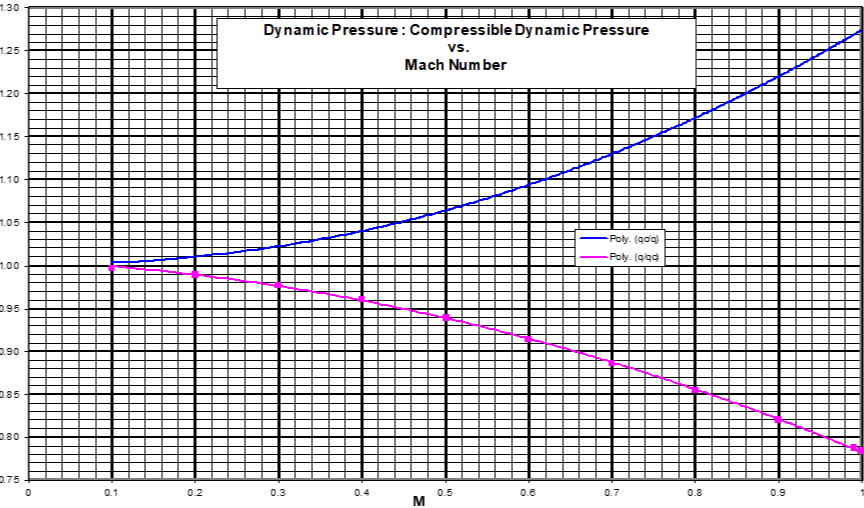
\includegraphics[width=8.99861in,height=5.29097in]{media/04/image8.png}

\hypertarget{supersonic-airspeed-and-mach-equations}{%
\section{Supersonic Airspeed and Mach Equations}\label{supersonic-airspeed-and-mach-equations}}

\(P_T'\) denotes pitot pressure behind shock wave

True Airspeed

\[ \frac{P_T' - P_a}{P_a} = \frac{q_c}{P_a} = \left[ \frac{\gamma + 1}{2} \left(  \frac{V}{a} \right)^2  \right]^\frac{\gamma}{\gamma-1} \left[ \frac{1}{ \frac{2\gamma}{\gamma+1} \left( \frac{V}{a} \right)^2 - \frac{\gamma-1}{\gamma+1} }  \right]^\frac{1}{\gamma-1} - 1 \]

Equivalent Airspeed (valid if \(q_c/P_a > 0.892 929 158\))

\[ \frac{q_c}{P_a} = \frac{166.92 \left[ \frac{V_e}{a_0 \sqrt{\sigma}} \right]^7} {\left( 7 \left[ \frac{V_e}{a_0 \sqrt{\sigma}} \right]^2 - 1 \right)^{2.5}} - 1 \]

Calibrated Airspeed (valid if \(V_c > a_0\))

\[ \frac{q_c}{P_0} = \frac{166.92 \left[ \frac{V_c}{a_0} \right]^7} {\left( 7 \left[ \frac{V_c}{a_0} \right]^2 - 1 \right)^{2.5}} - 1\]

Mach Number

\[ \frac{q_c}{P_a} = \frac{166.92 M^7} {\left( 7 M^2 - 1 \right)^{2.5}} -1 \]

\hypertarget{total-temperature-equation}{%
\section{Total Temperature Equation}\label{total-temperature-equation}}

Since stagnation exists at the probe, it absorbs the energy of the air

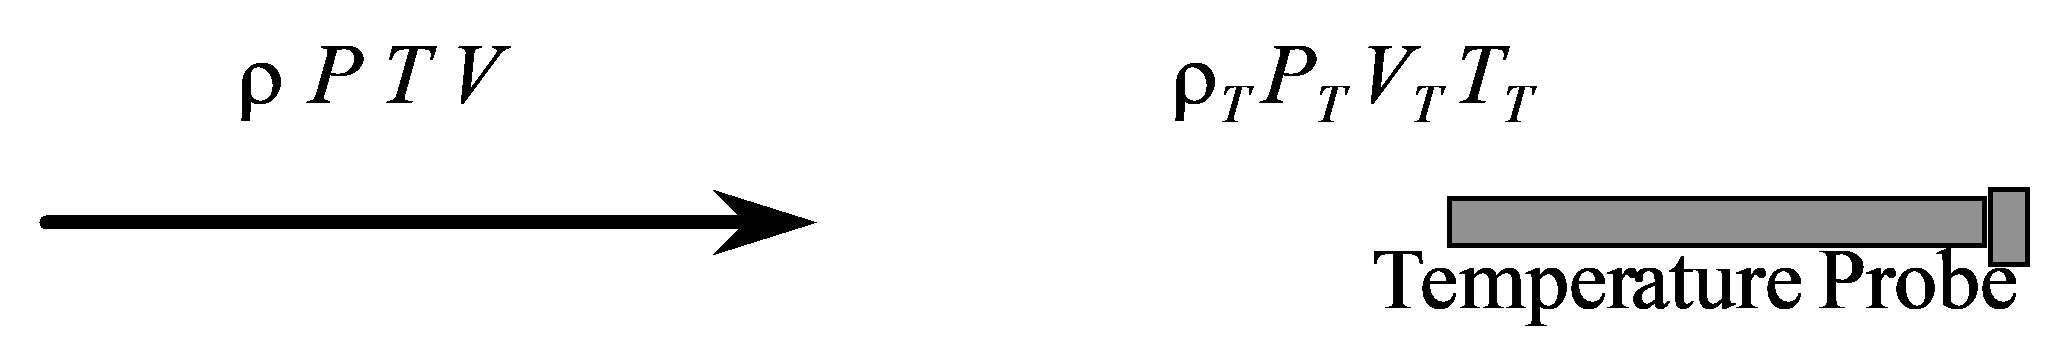
\includegraphics[width=5in,height=0.82in]{media/04/image13.png}

Apply Bernoulli:

\[ \frac{V^2}{2} + \frac{\gamma}{\gamma - 1}  \frac{P_s}{\rho_s} = \frac{\gamma}{\gamma - 1} \frac{P_p}{\rho_p} \]

Also \(\frac{P}{\rho} = RT\) and \(a^2 = \gamma RT\) therefore

\[ \frac{T_T}{T_a} = 1 + \left[ \frac{\gamma - 1}{2} \right] M^2 \]

Use \emph{K} (probe recovery factor) to account for heat losses:

\[ \frac{T_T}{T_a} = 1 + \left[ \frac{K(\gamma - 1)}{2} \right] M^2 \]

During position error flight testing, measure \(T_i\). From \(V_c\) and \(H_{\mathrm{pc}}\) determine M

\[ T_i + \Delta T_{\mathrm{ic}} = T_T = T_a + T_aKM^2 \]

Plot \(T_i\) vs \(M^2\)

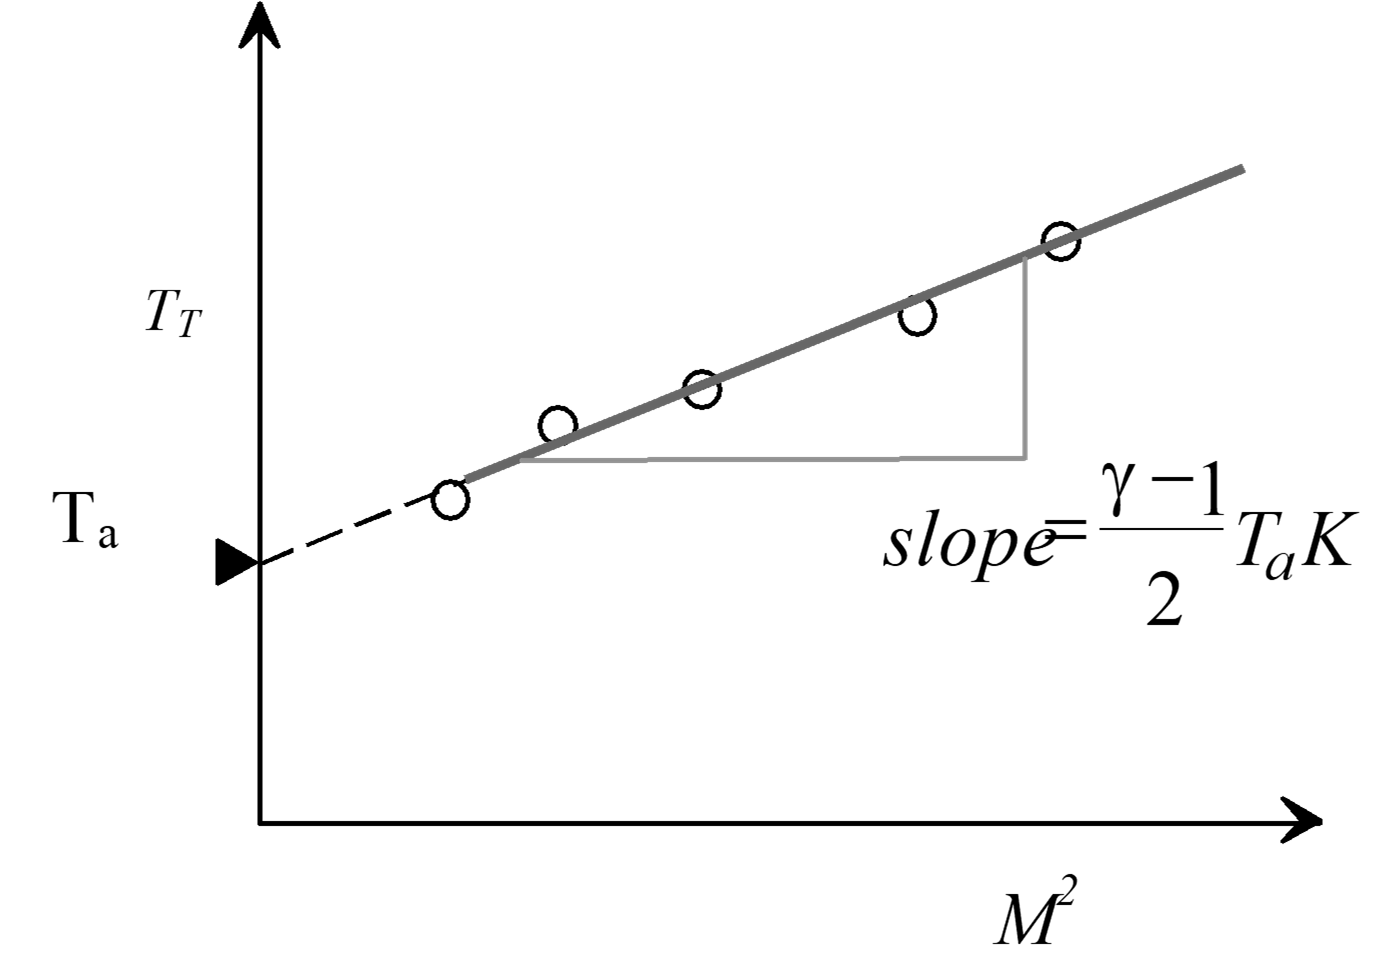
\includegraphics[width=4.3125in,height=3in]{media/04/image14.png}

\hypertarget{altimeter-equation}{%
\section{Altimeter Equation}\label{altimeter-equation}}

\(P_a = P_0 \left(1-6.875 35 \times 10^{-6} H\right)^{5.256}\) below 36,089 ft

\(P_a = P_0 \left(0.223 35 \right) \textrm{e}^{-0.000 048 06[H-36089]}\) above 36,089 ft

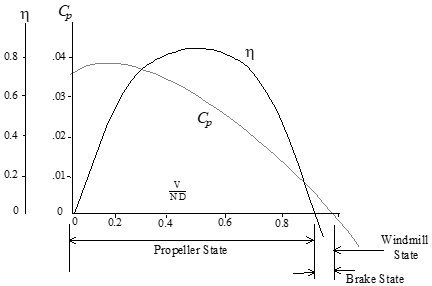
\includegraphics[width=4.20347in,height=4.11319in]{media/04/image15.png}

\begin{longtable}[]{@{}ll@{}}
\toprule
Symbol & Definition\tabularnewline
\midrule
\endhead
\(H_i\) & indicated pressure altituide (29.92" Hg)\tabularnewline
\(\Delta H_{\mathrm{ic}}\) & instrument error correction\tabularnewline
\(H_{\mathrm{ic}}\) & altimeter corrected of instrument error\tabularnewline
\(\Delta H_{\mathrm{pc}}\) & position error correction\tabularnewline
\(H_c\) & calibrated pressure altitude\tabularnewline
\bottomrule
\end{longtable}

\hypertarget{position-error-test-methods}{%
\section{Position Error Test Methods}\label{position-error-test-methods}}

\hypertarget{fly-by}{%
\subsection{Fly-by}\label{fly-by}}

As depicted below, the flyby method originally used some sort of viewing platform with surveyed distances and a grid or other device for determining the aircraft's relative angle above the platform's altimeter. This information combined to give the aircraft's actual pressure altitude. Modern methods replace the tower system with a radar altimeter or GPS unit to determine tapeline height above the flyby line (\(H_g\)). This geometric height is converted to a pressure altitude change using a temperature correction. When added to the aircraft's pressure altitude on the runway, this change provides the actual pressure altitude during the flyby (\(\textrm{Actual } H_c = \textrm{runway pressure altitude} + H_g (T_s/T_t)\)).

\includegraphics[width=5.28681in,height=1.76042in]{media/04/image17.png}

\[\text{Actual } H_{c} = H_{c_{\mathrm{tower}}} + \left( D\tan\theta \cdot \frac{T_{s}}{T_{t}} \right) \]

\[ \Delta H_{\mathrm{pc}} = \text{Actual } H_c - \left( H_i + \Delta H_{\mathrm{ic}} \right) \]

\[ \Delta P_s = \rho g \Delta H_{\mathrm{pc}} \]

\[ \Delta P_{S} = q_{c} - q_{\mathrm{cic}} \]

\[ \Delta P_{S} = \frac{1}{2}\rho_{0}{V_{c}^{2} - \frac{1}{2}\rho_{0}{V_{\mathrm{ic}}}^{2} \text{ (low Mach only)}} \]

Solve for \(V_c\)

\[ \Delta V_{\mathrm{pc}} = V_c - V_{\mathrm{ic}} \]

See flowchart for high mach or \(P_T \ne 0\) cases.

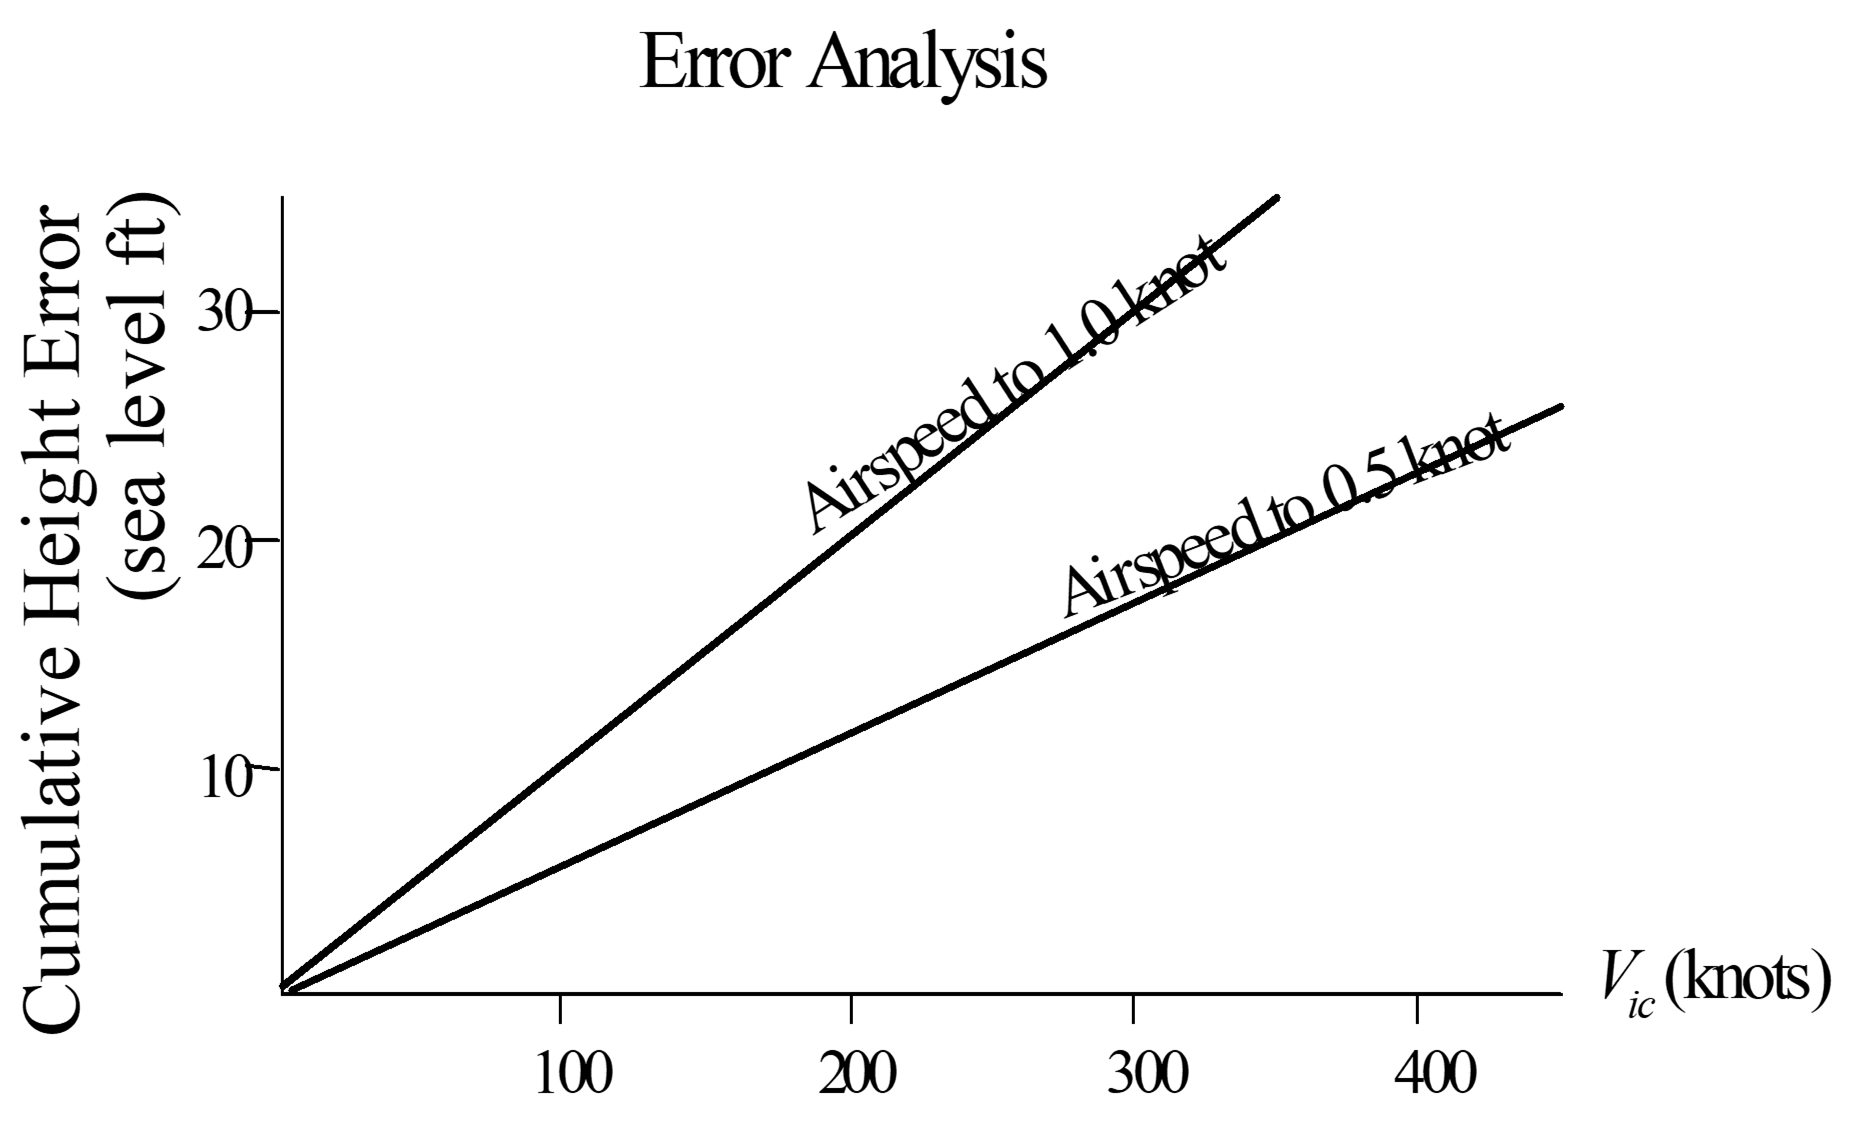
\includegraphics[width=5.1875in,height=3.15in]{media/04/image18.png}

Note: A check on basic instrument calibration is easily accomplished using a ``ground block'' where a parked test aircraft compares altimeters with tower. Any error can be treated as a bias.

This altitude-based test method determines altimeter corrections and therefore static error directly. Accurately converting this static source error to an airspeed correction also requires knowledge of the test pitot tube's total pressure error (\(\Delta P_T\) ). This can be determined either through direct comparison with a calibrated noseboom pitot pressure or from one of the airspeed-based methods that directly yield airspeed corrections (pace, ground course, GPS). In lieu of these options, the pitot error may assumed to be zero, but this will reduce confidence in the calculated value for airspeed correction.

\hypertarget{ground-course-method}{%
\subsection{Ground Course Method}\label{ground-course-method}}

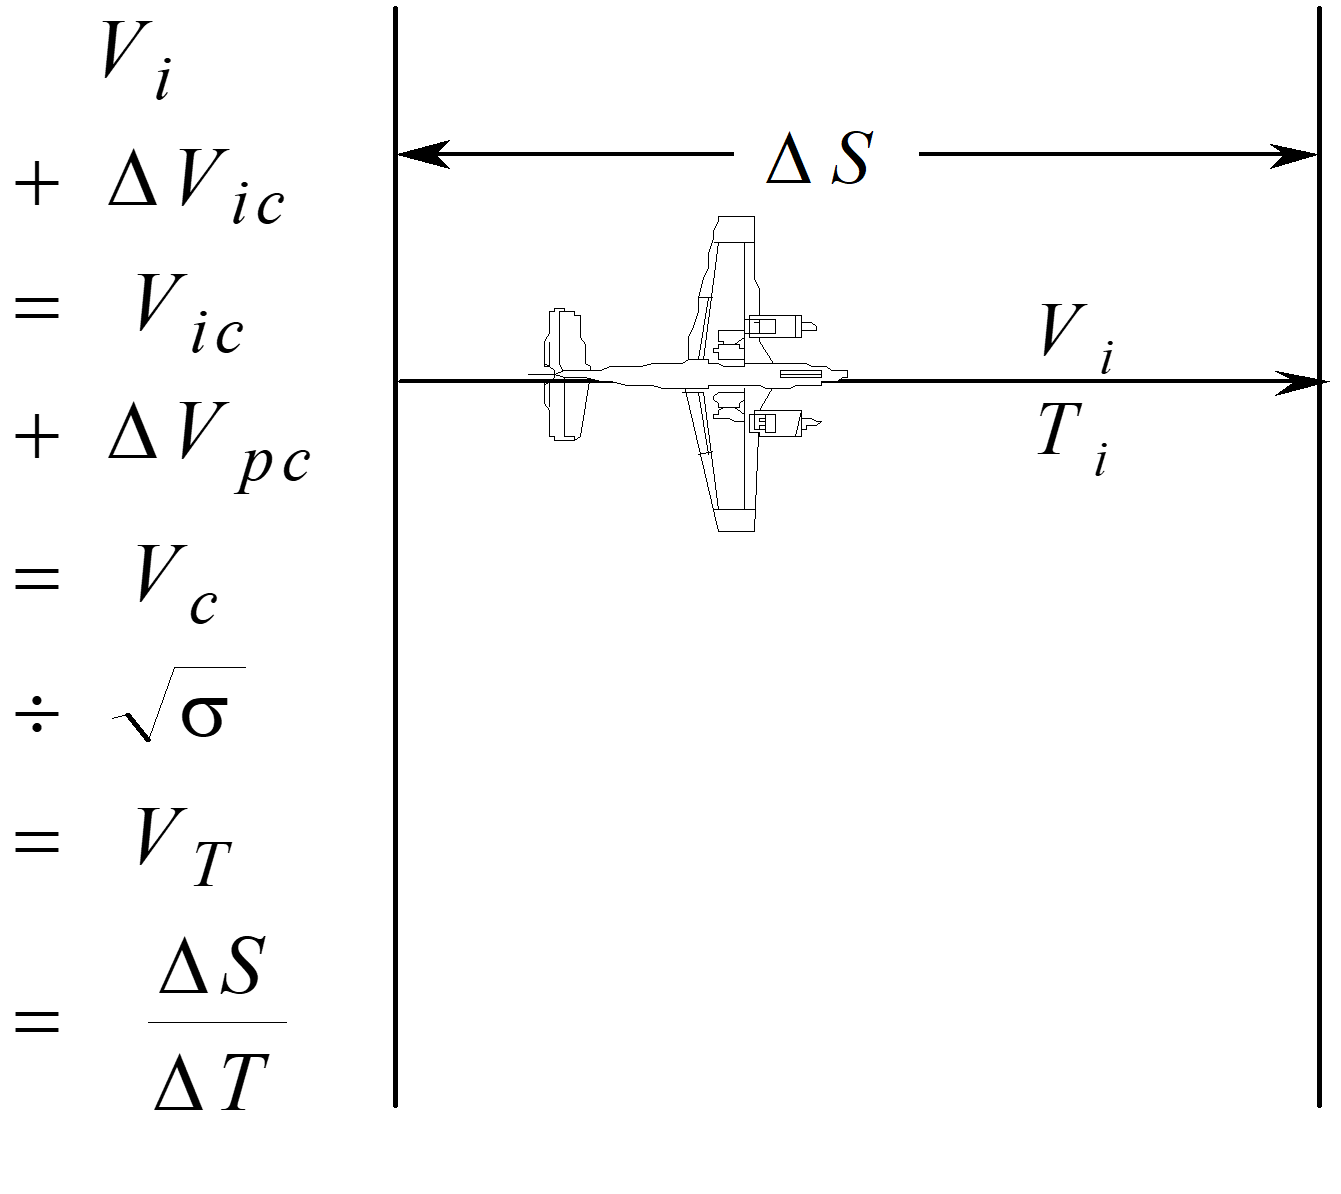
\includegraphics[width=4.5625in,height=4.0625in]{media/04/image19.png}

Fly known course at constant \(V_i\)

Elapsed time = \(\Delta T\), therefore \(V_T = \frac{\Delta S}{\Delta T}\)

Use \(H_i\) and \(T_i\) to compute \(V_e = V_T \left(\sqrt{\sigma} \right) = V_c\) for low altitude

Correct \(V_i\) for instrument error corrections (\(\Delta V_{\mathrm{ic}}\)) using

\[V_{\mathrm{ic}} = V_i + \Delta V_{\mathrm{ic}} \]

\[\Delta V_{\mathrm{pc}} = V_c - V_{\mathrm{ic}} \]

To determine altimeter error assume \(\Delta P_T = 0\)

\[\frac{1}{2} \rho_0 \left[ V_c^2 - V_{\mathrm{ic}}^2 \right] = +\Delta P_s \]

\[\Delta P_s = +\rho g \Delta H \]

If \(\Delta P_T \ne 0\), then \(\Delta H_{\mathrm{pc}} = + \frac{\Delta P_s - \Delta P_T}{\rho g}\)

Error resulting from a \(\frac{1}{2}\) sec timing error

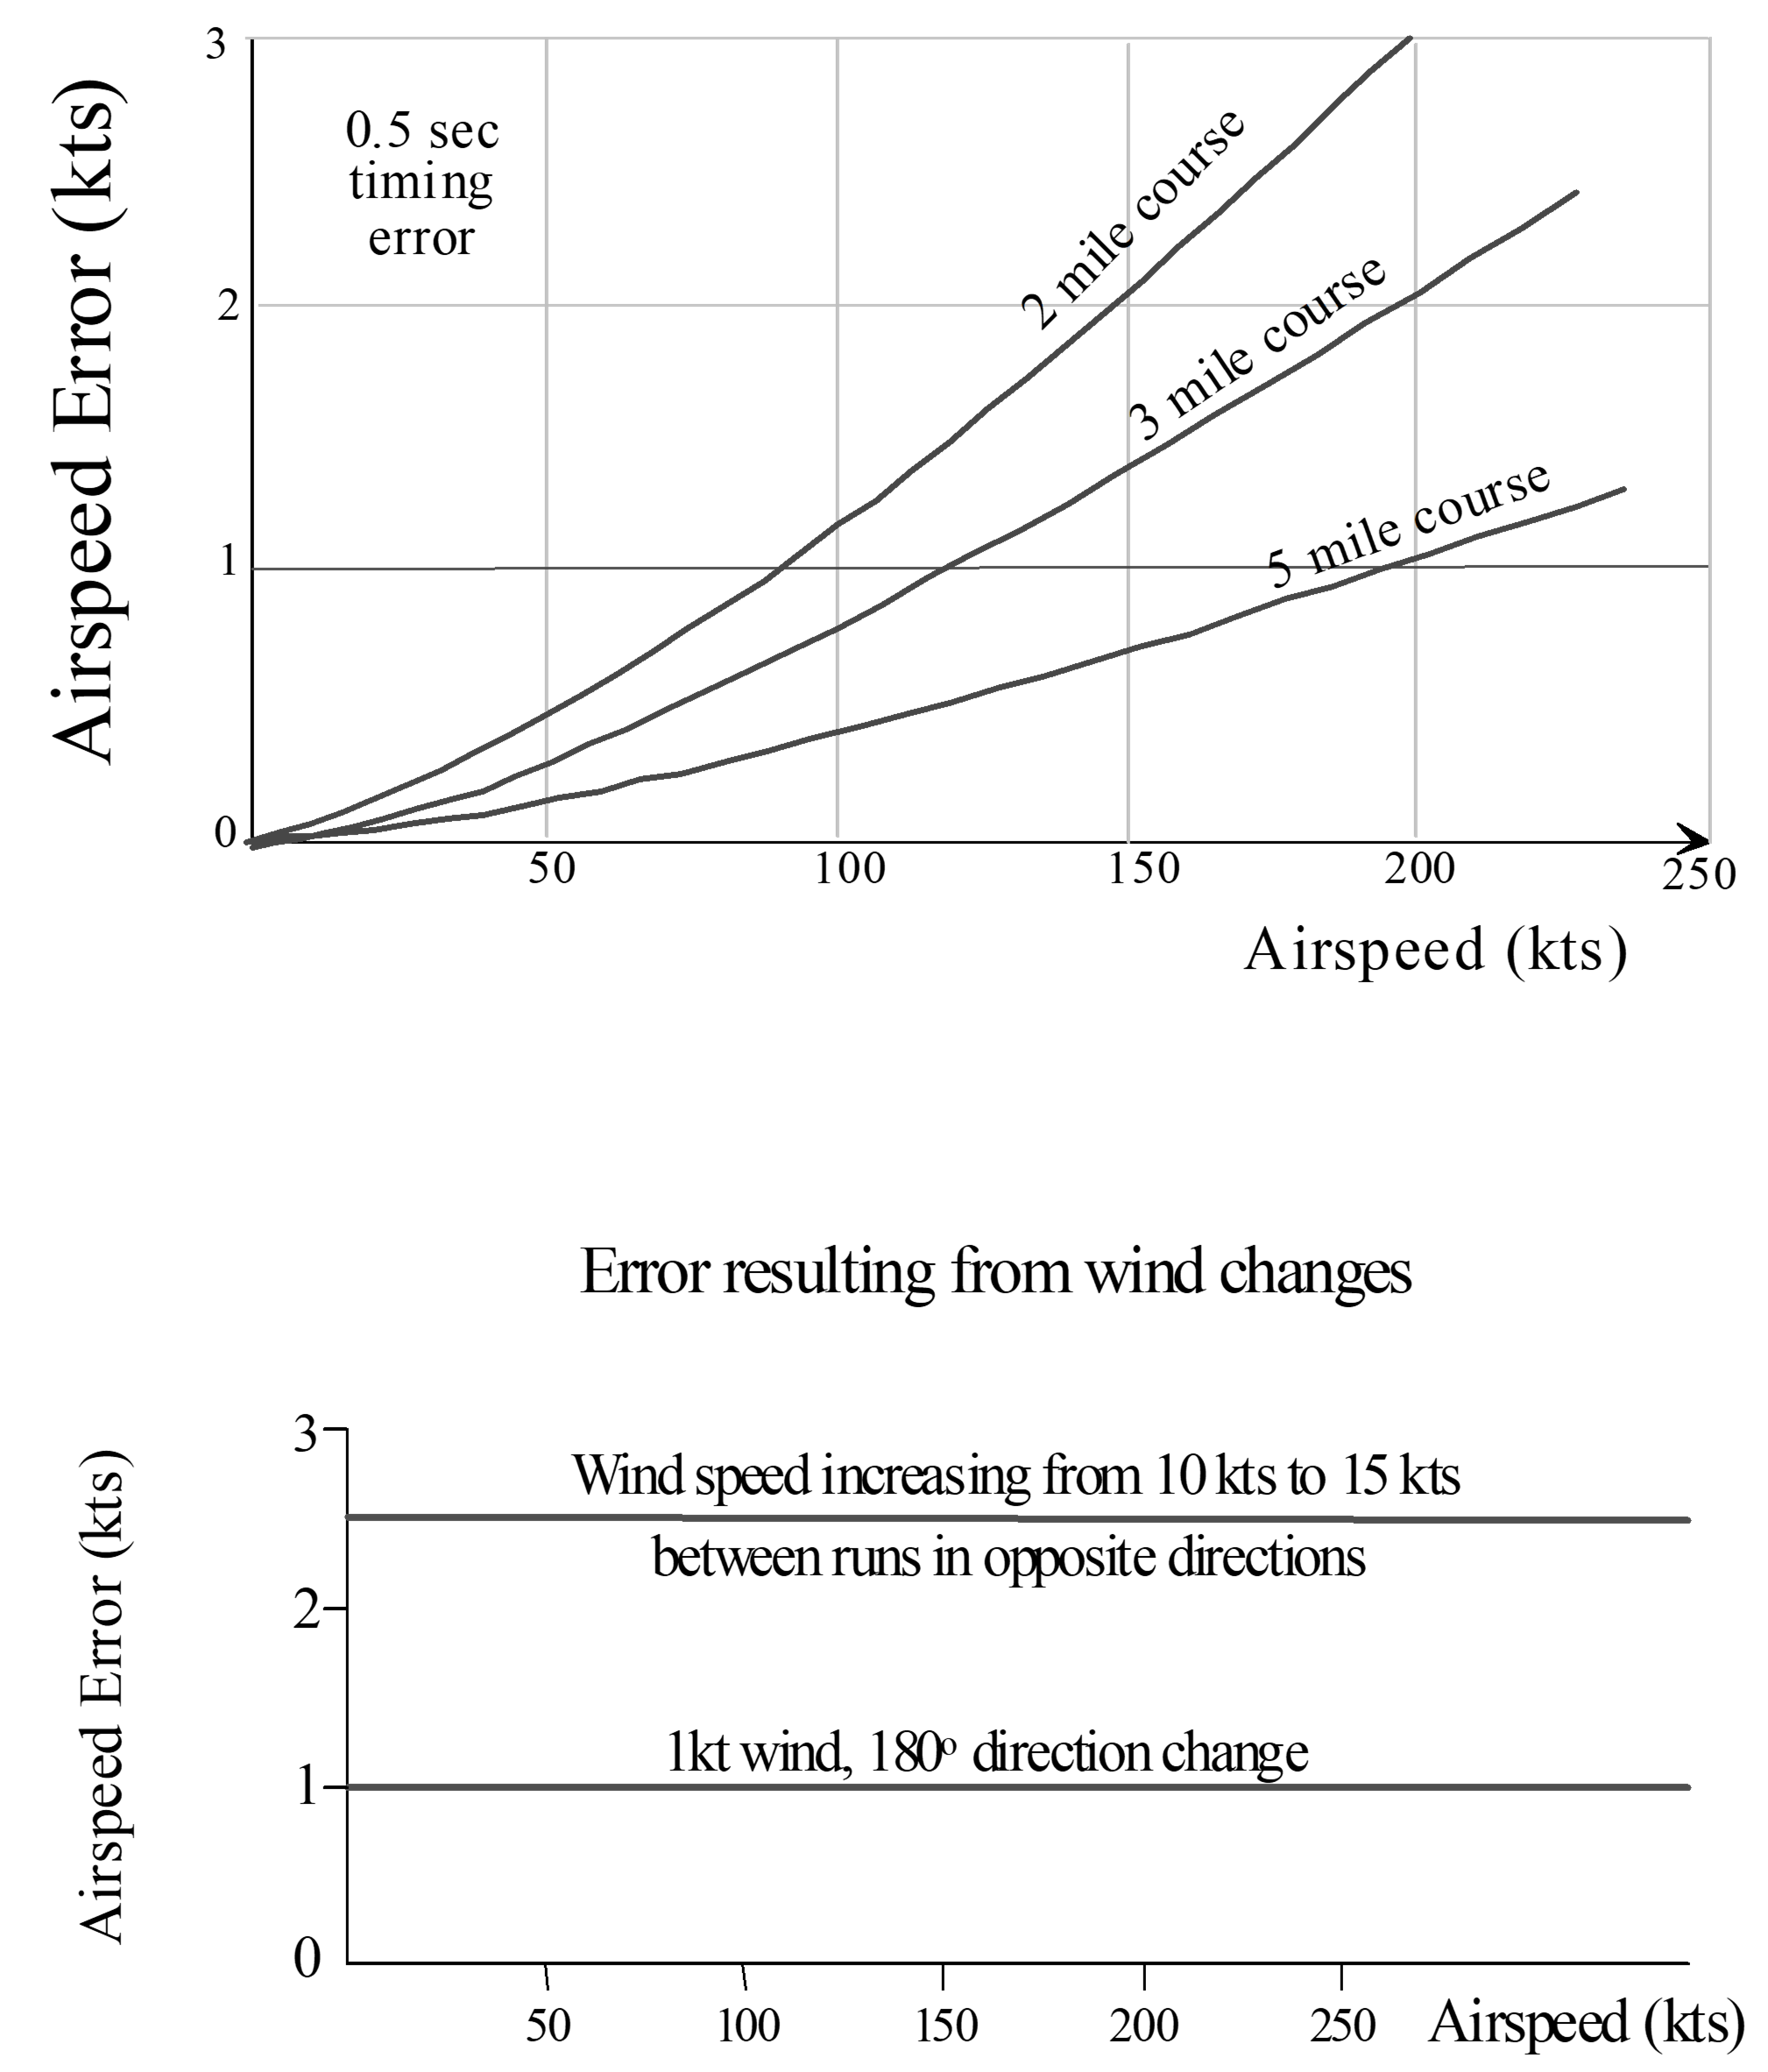
\includegraphics[width=5.5125in,height=6.4625in]{media/04/image21.png}

This airspeed-based test method determines airspeed corrections directly. Accurately converting this airspeed error to a static source error requires knowledge of the test pitot tube's total pressure error (\(\Delta P_T\)). This can be determined using one of the altitude-based methods that directly yield altitude corrections (tower fly-by, trailing cone or bomb). In lieu of these options, the pitot error may assumed to be zero, but this will reduce confidence in the calculated values for static pressure error and altimeter correction.

\hypertarget{trailing-conebomb-method}{%
\subsection{Trailing Cone/Bomb Method}\label{trailing-conebomb-method}}

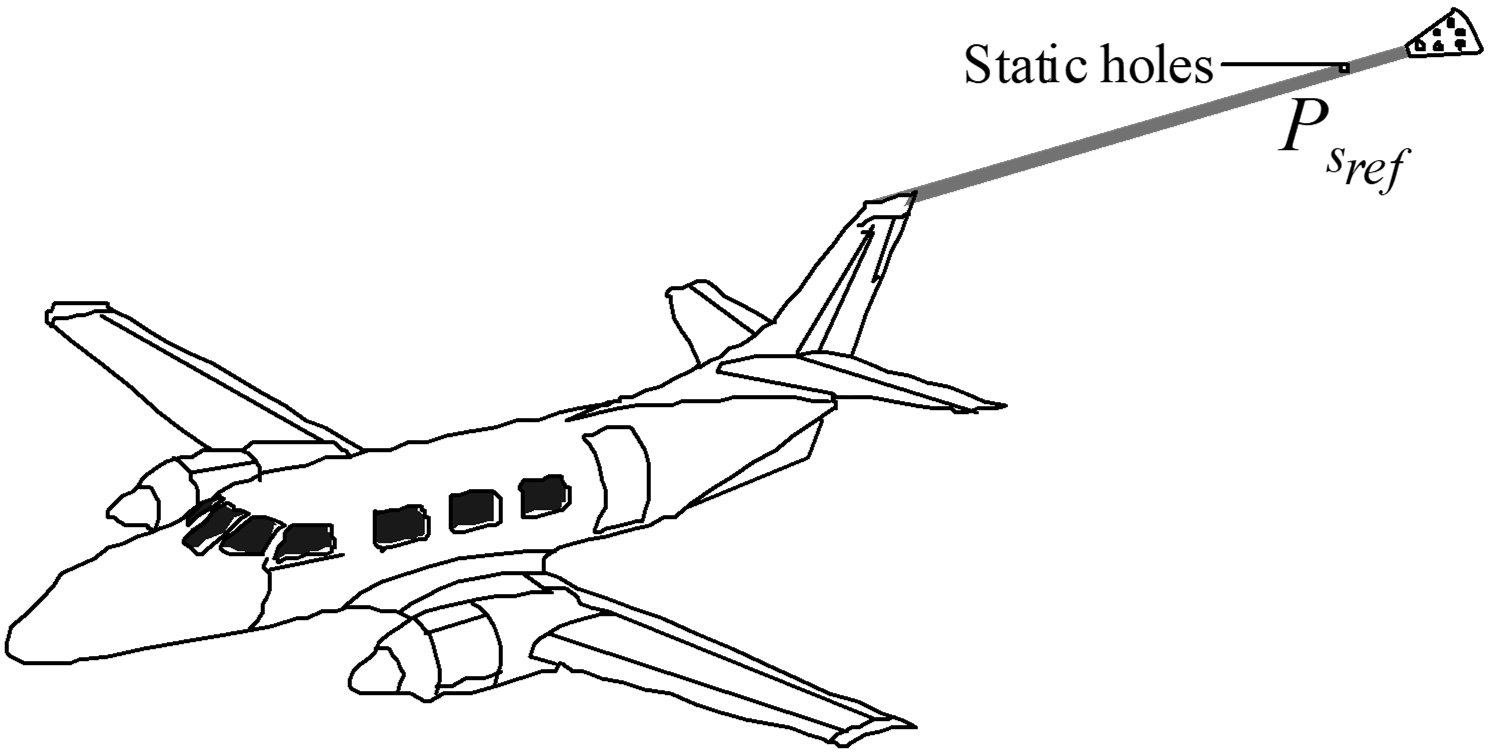
\includegraphics[width=5.9375in,height=3in]{media/04/image23.png}

\begin{enumerate}
\def\labelenumi{\arabic{enumi}.}
\tightlist
\item
  Measure \(P_s\) (ref) away from pressure field of aircraft
\item
  Cone is used to stabilize static line
\item
  No speed limitations
\item
  Inexpensive---can be trailed on landing
\item
  Consider lag effects during rapid altitude changes
\end{enumerate}

\(\Delta P_s = \Delta P_{s_{\mathrm{A/C}}} - \Delta P_{s_{\mathrm{REF}}}\)

\(\Delta H_{\mathrm{pc}} = +\frac{\Delta P_s}{\rho g} = \textrm{altimeter correction}\)

\(\Delta P_T - \Delta P_s = \Delta P_D = q_{\mathrm{ic}} - q_c \text{ assuming } \Delta P_T = 0 \text{ , } M < 0.2\)

If pitot errors do exist, then they must be included in calculations for \(\Delta V_{\mathrm{pc}}\) (see flowchart).

Using a trailing cone during stall testing may give airspeed errors due to lag errors during the deceleration.

This altitude-based test method determines altimeter corrections and therefore static error directly. Accurately converting this static source error to an airspeed correction also requires knowledge of the test pitot tube's total pressure error (\(\Delta P_T\)). This can be determined either through direct comparison with a calibrated noseboom pitot pressure or from one of the airspeed-based methods that directly yield airspeed corrections (pace, ground course, GPS). In lieu of these options, the pitot error may assumed to be zero, but this will reduce confidence in the calculated value for airspeed correction.

\hypertarget{gps-methods}{%
\subsection{GPS Methods}\label{gps-methods}}

The attraction

\begin{itemize}
\tightlist
\item
  no aircraft modifcations required

  \begin{itemize}
  \tightlist
  \item
    no trailing cone or aircraft plumbing mod
  \item
    no flight test boom
  \end{itemize}
\item
  no limitation on speed or altitude

  \begin{itemize}
  \tightlist
  \item
    can be done down to near stall
  \item
    any altitude
  \end{itemize}
\item
  easy data reduction

  \begin{itemize}
  \tightlist
  \item
    no correlation with pace aircraft, ground radar, or other references required
  \end{itemize}
\end{itemize}

Various methods available, all assume \textbf{steady} winds and ambient temperature. You must determine wind speed and direction to calculate \(V_T\) and \(T_0\) and to ensure steady winds existed during test series.

GPS accuracies are variable. Know tolerances before accepting GPS as a truth model.

If exact (\(\pm 10°\)) winds are calculated inflight, you can fly one pass directly into/away from the wind

\[V_T = V_G + V_{Headwind}\]

This airspeed-based test method determines airspeed corrections directly. Accurately converting this airspeed error to a static source error requires knowledge of the test pitot tube's total pressure error (\(\Delta P_T\)). This can be determined using one of the altitude-based methods that directly yield altitude corrections (tower fly-by, trailing cone or bomb). In lieu of these options, the pitot error may assumed to be zero, but this will reduce confidence in the calculated values for static pressure error and altimeter correction.

\emph{Graphs in Section 4.11 separately show the effect of measurement errors in \(\Delta P_T\), air temperature, or true airspeed on \(\Delta V_c\) calculations . The last chart of this Section shows how each knot of accumulated \(\Delta V_c\) uncertainty affects the \(\Delta H_c\) uncertainty at various altitudes and temperatures.}

Flying four legs instead of three allows four separate calculations of wind speed \& direction to confirm stable winds at that test airspeed. If several real-time calculations of winds confirm constant direction and velocity, then testing may be shortened by flying only one pass directly into or away from the wind. If this is done, an end-of-test wind calibration must be performed to confirm steady winds throughout the test series. To minimize temperature and wind variations, testing should be accomplished within a relatively small area.

\hypertarget{horseshoe-track-gps-method}{%
\subsubsection*{Horseshoe Track GPS Method}\label{horseshoe-track-gps-method}}
\addcontentsline{toc}{subsubsection}{Horseshoe Track GPS Method}

\begin{itemize}
\tightlist
\item
  Horseshoe track method

  \begin{itemize}
  \tightlist
  \item
    fly three legs with each perpedicular ground tracks, noting GPS ground speed on each
  \item
    determine true airspeed by solving three equations in three unknowns
  \end{itemize}
\item
  Practical problem

  \begin{itemize}
  \tightlist
  \item
    need to fly close to the ground, tracking perpendicular ground references
  \end{itemize}
\end{itemize}

\includegraphics[width=2.7in,height=2.49514in]{media/04/image28.png}

True airspeed: \(V_T = \frac{1}{2} \sqrt{V_1^2 + V_2^2 + V_3^2 + V_1^2 \times \frac{V_3^2}{V_2^2}}\)

Wind velocity: \(V_W = \sqrt{\left( \frac{V_1 - V_3}{2} \right)^2 + \left( \frac{V_2 - V_1 \times V_3 / V_2}{2} \right) ^2 }\)

Wind direction: \(\psi_W = \tan^{-1} \frac{V_2 - V_1 \times V_3 / V_2}{V_1 - V_3}\)

\hypertarget{horseshoe-heading-gps-method}{%
\subsubsection*{Horseshoe Heading GPS Method}\label{horseshoe-heading-gps-method}}
\addcontentsline{toc}{subsubsection}{Horseshoe Heading GPS Method}

\begin{itemize}
\tightlist
\item
  Horseshoe Heading Method

  \begin{itemize}
  \tightlist
  \item
    Fly three legs with perpendicular headings, noting GPS ground speed on each
  \item
    Determine true airspeed by solving three equations in three unknowns
  \end{itemize}
\end{itemize}

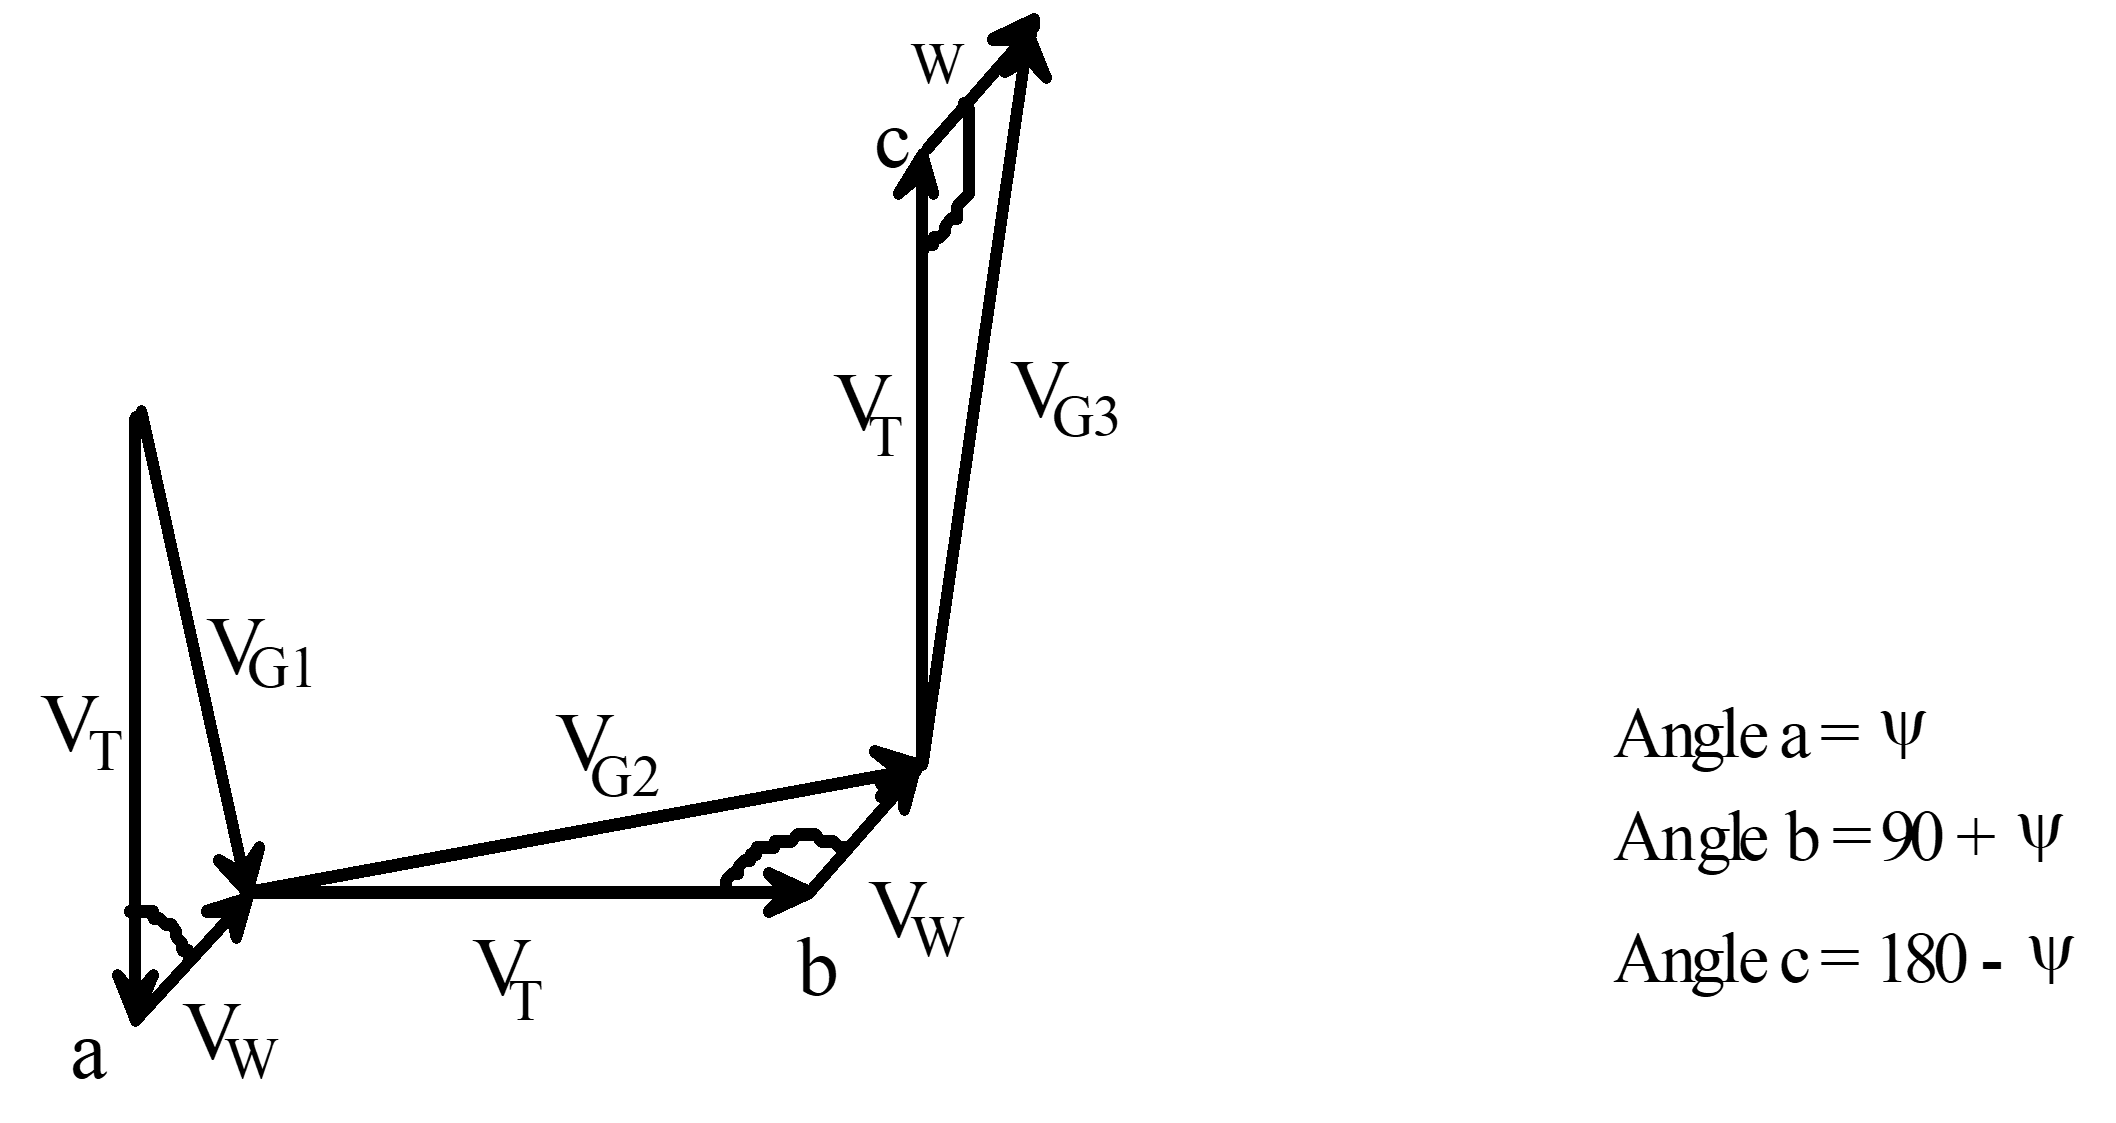
\includegraphics[width=5.0625in,height=2.6875in]{media/04/image31.png}

Wind direction: \(\psi = \tan^{-1} \frac{-V_{G1}^2 + 2V_{G2}^2 - V_{G3}^2}{V_{G3}^2 - V_{G1}^2}\)

Wind velocity: \(V_W = \frac{1}{2} \left[ V_{G3}^2 + V_{G1}^2 \pm \sqrt{ \left(V_{G3}^2 + V_{G1}^2 \right)^2 \pm \left( \frac{-V_{G1}^2 + 2V_{G2}^2 - V_{G3}^2}{\sin{\psi}} \right)^2 } \right]^{1/2}\)

True airspeed: \(V_T = \sqrt{\frac{V_{G3}^2 + V_{G1}^2}{2} - V_W^2}\)

The ``Windbox'' method consists of flying four legs instead of three. The extra leg provides a fourfold increase in wind calculations to improve result confidence. The ``Orbis'' method extends this advantage by collecting data at every heading throughout a level turn.

\hypertarget{cloverleaf-method}{%
\subsubsection*{Cloverleaf Method}\label{cloverleaf-method}}
\addcontentsline{toc}{subsubsection}{Cloverleaf Method}

(Microsoft Excel spreadsheet adapted from Doug Gray, NSW Australia)

\begin{itemize}
\tightlist
\item
  Fly three legs with approximately 90-120 degree difference between headings.

  \begin{itemize}
  \tightlist
  \item
    Can be accomplished in a broad turn as with the horseshoe method, or
  \item
    Directly over a single point (cloverleaf maneuver).
  \end{itemize}
\item
  Accurate results require

  \begin{itemize}
  \tightlist
  \item
    Identical values for indicated airspeed (and TAS) for all legs.
  \item
    Constant winds throughout data collection (single W/S vector in figure).
  \item
    Approx. 10 seconds stable ground speed, Vg, (G/S in figure) during each leg.
  \end{itemize}
\item
  Aircraft heading results for each leg entail an airborne compass swing.
\end{itemize}

\begin{longtable}[]{@{}l@{}}
\toprule
Inputs for each 3-leg data set\tabularnewline
\midrule
\endhead
\(V_{g_1}\) \(V_{g_2}\) \(V_{g_3}\)\tabularnewline
\(Trk_{1}\) \(Trk_{2}\) \(Trk_{3}\)\tabularnewline
\bottomrule
\end{longtable}

\begin{longtable}[]{@{}l@{}}
\toprule
Intermediate calculations\tabularnewline
\midrule
\endhead
\(X_1 = V_{g_1} * \sin(\pi * (360 - Trk_1) / 180)\)\tabularnewline
\(Y_1 = V_{g_1} * \cos(\pi * (360 - Trk_1) / 180)\)\tabularnewline
\(X_2 = V_{g_2} * \sin(\pi * (360 - Trk_2) / 180)\)\tabularnewline
\(Y_2 = V_{g_2} * \cos(\pi * (360 - Trk_2) / 180)\)\tabularnewline
\(X_3 = V_{g_3} * \sin(\pi * (360 - Trk_3) / 180)\)\tabularnewline
\(Y_3 = V_{g_3} * \cos(\pi * (360 - Trk_3) / 180)\)\tabularnewline
\(M_1 = -(X_2 - X_1) / (Y_2 - Y_1)\)\tabularnewline
\(M_2 = -(X_3 - X_1) / (Y_3 - Y_1)\)\tabularnewline
\(B_1 = (Y_1 + Y_2)/2 - M_1 * (X_1 + X_2) / 2\)\tabularnewline
\(B_2 = (Y_1 + Y_3)/2 - M_2 * (X_1 + X_3) / 2\)\tabularnewline
\(V_{W_x} = (B_1 - B_2) / (M_2 - M_1)\)\tabularnewline
\(V_{w_y} = M_1 * V_{W_x} + B_1\)\tabularnewline
\bottomrule
\end{longtable}

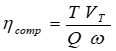
\includegraphics[width=5in,height=3.4in]{media/04/image32.png}

\begin{longtable}[]{@{}l@{}}
\toprule
\begin{minipage}[b]{0.97\columnwidth}\raggedright
Results\strut
\end{minipage}\tabularnewline
\midrule
\endhead
\begin{minipage}[t]{0.97\columnwidth}\raggedright
Aircraft true airspeed \(= V_T = \left[\left(X_1 - V_{W_x}\right)^2 + \left(Y_1 - V_{W_y}\right)^2 \right]^{0.5}\)\strut
\end{minipage}\tabularnewline
\begin{minipage}[t]{0.97\columnwidth}\raggedright
Total wind speed \(= V_W = \left[\left(V_{W_x}^2 + V_{W_y}^2\right)\right]^{0.5}\)\strut
\end{minipage}\tabularnewline
\begin{minipage}[t]{0.97\columnwidth}\raggedright
Wind direction \(= \psi_W = Psi_W = \mod(540 - (180/\pi * \textrm{ATAN2}(V_{W_y}, V_{W_x})), 360)\)\strut
\end{minipage}\tabularnewline
\begin{minipage}[t]{0.97\columnwidth}\raggedright
1\textsuperscript{st} leg a/c heading \(= \psi_1 = Psi_1 = \mod(540 - (180/\pi * \textrm{ATAN2}(V_{W_y}-Y_1, V_{W_x}-X_1)), 360)\)\strut
\end{minipage}\tabularnewline
\begin{minipage}[t]{0.97\columnwidth}\raggedright
2\textsuperscript{nd} leg a/c heading \(= \psi_2 = Psi_2 = \mod(540 - (180/\pi * \textrm{ATAN2}(V_{W_y}-Y_2, V_{W_x}-X_2)), 360)\)\strut
\end{minipage}\tabularnewline
\begin{minipage}[t]{0.97\columnwidth}\raggedright
3\textsuperscript{rd} leg a/c heading \(= \psi_3 = Psi_3 = \mod(540 - (180/\pi * \textrm{ATAN2}(V_{W_y}-Y_3, V_{W_x}-X_3)), 360)\)\strut
\end{minipage}\tabularnewline
\bottomrule
\end{longtable}

\hypertarget{position-error-far-2325.1323-and-.1325jar-certification}{%
\section{Position Error FAR 23/25.1323 and .1325/JAR Certification}\label{position-error-far-2325.1323-and-.1325jar-certification}}

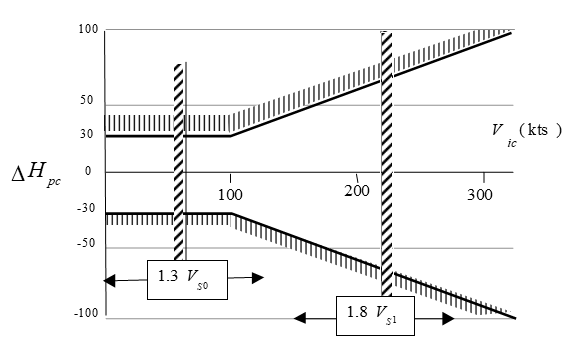
\includegraphics{media/04/image47.png}

\begin{itemize}
\tightlist
\item
  Requirements

  \begin{itemize}
  \tightlist
  \item
    Maximum error at sea level must be less than \(\pm 30 \text{ft}/100 \text{kts}\) between \(1.3 V_{\mathrm{SO}}\) and \(1.8 V_{S1}\)
  \item
    \(V_{S0} =\) Full flap, gear down, power off, stall speed )
  \item
    \(V_{S1} =\) Stall speed in a specific configuration )
  \end{itemize}
\end{itemize}

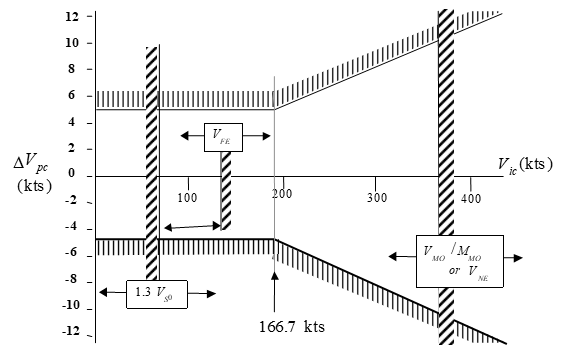
\includegraphics{media/04/image48.png}

Errors must be equal to or less than \(\pm3\%\) of \(V_c\) or \(\pm5\text{kts}\) whichever is greater

\hypertarget{mil-spec-p-26292-c-usaf}{%
\subsubsection*{Mil Spec P-26292 C (USAF)}\label{mil-spec-p-26292-c-usaf}}
\addcontentsline{toc}{subsubsection}{Mil Spec P-26292 C (USAF)}

Landing configuration: \(\Delta H_{\mathrm{pc}} \pm 30\) ft.

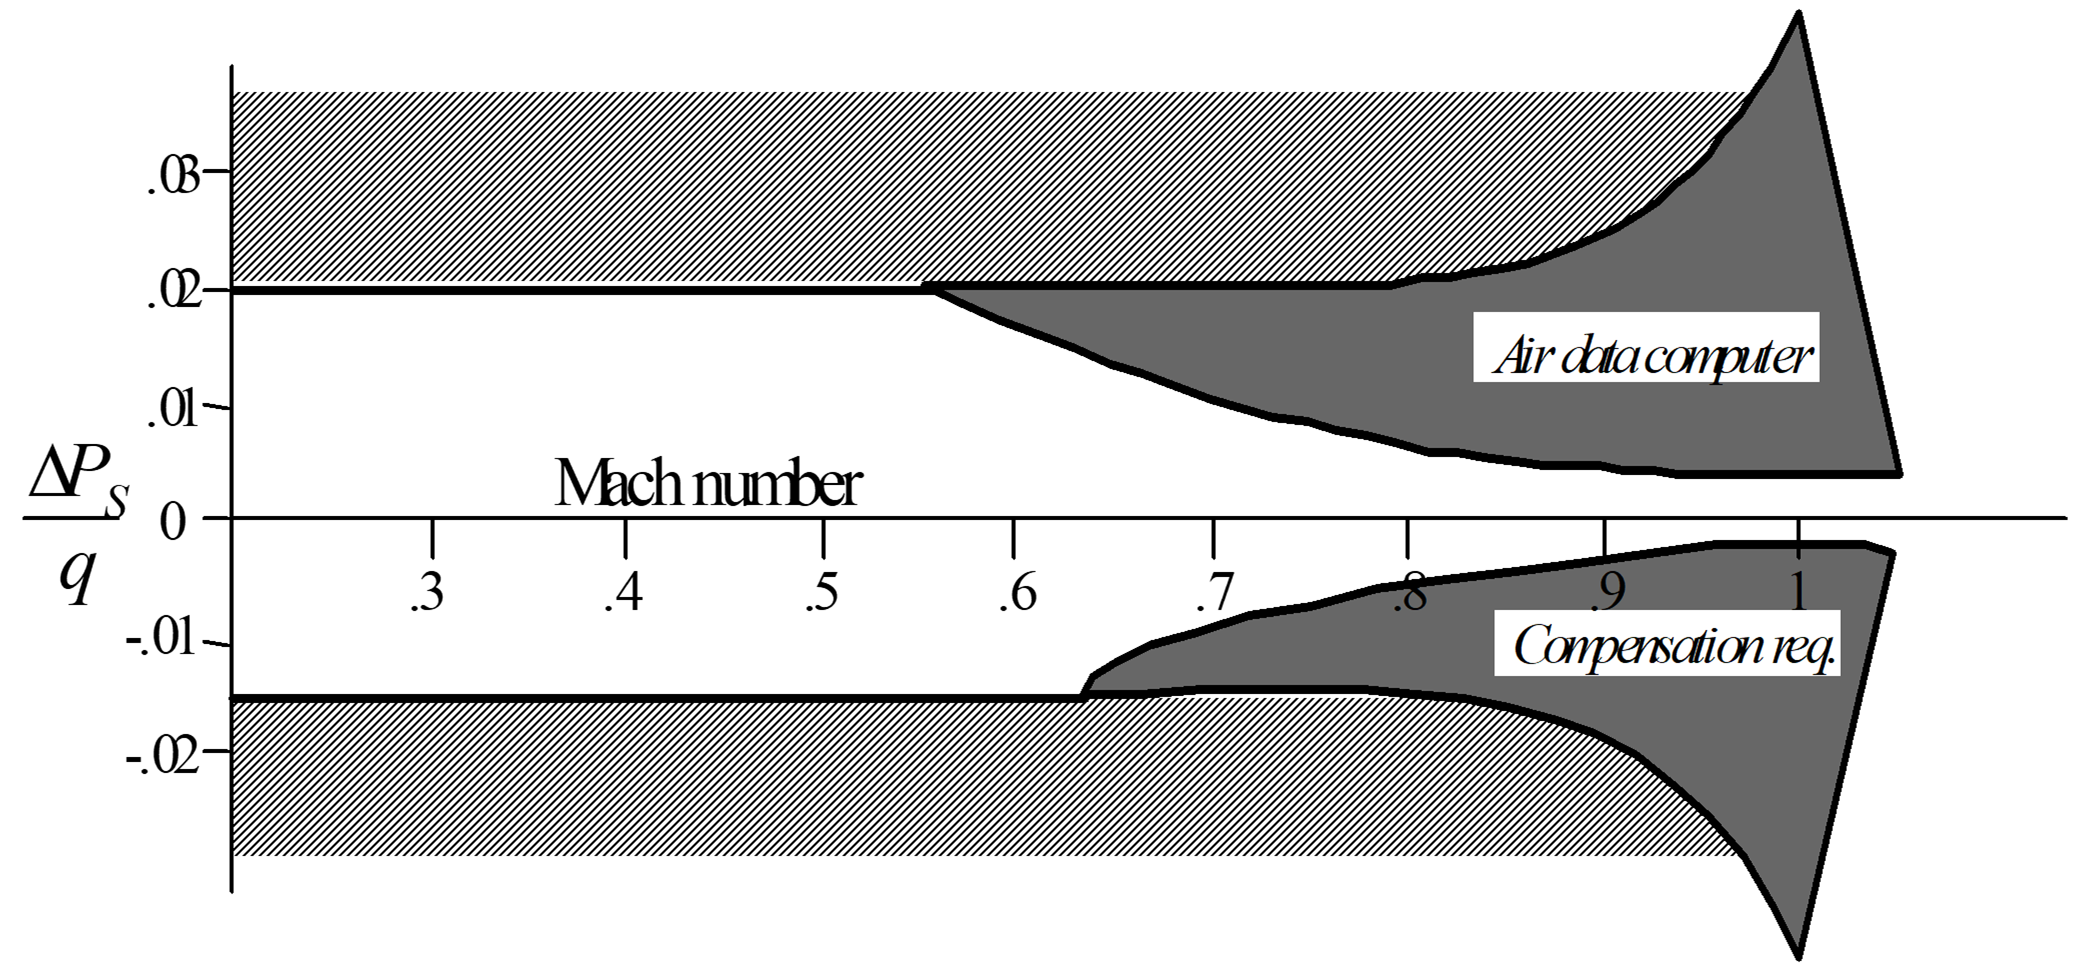
\includegraphics[width=5.75in,height=2.6875in]{media/04/image50.png}

\hypertarget{pec-correction-process-flow-chart}{%
\section{PEC Correction Process Flow Chart}\label{pec-correction-process-flow-chart}}

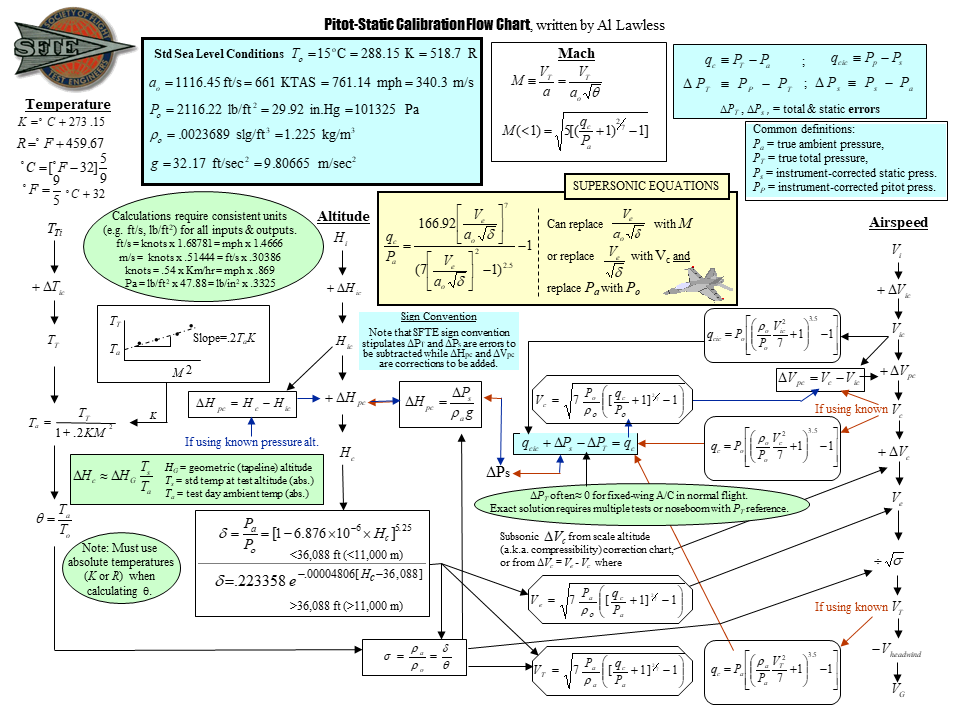
\includegraphics[width=8.63072in,height=6.4465in]{media/04/image52.png}

\hypertarget{airspeedaltitudemach-graphic-relation}{%
\section{Airspeed/Altitude/Mach Graphic Relation}\label{airspeedaltitudemach-graphic-relation}}

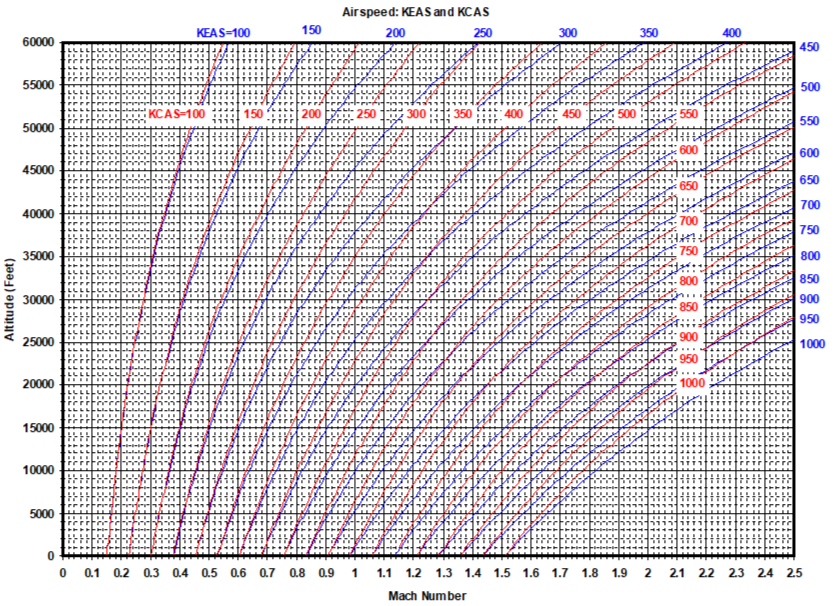
\includegraphics[width=8.68611in,height=6.31181in]{media/04/image53.png}

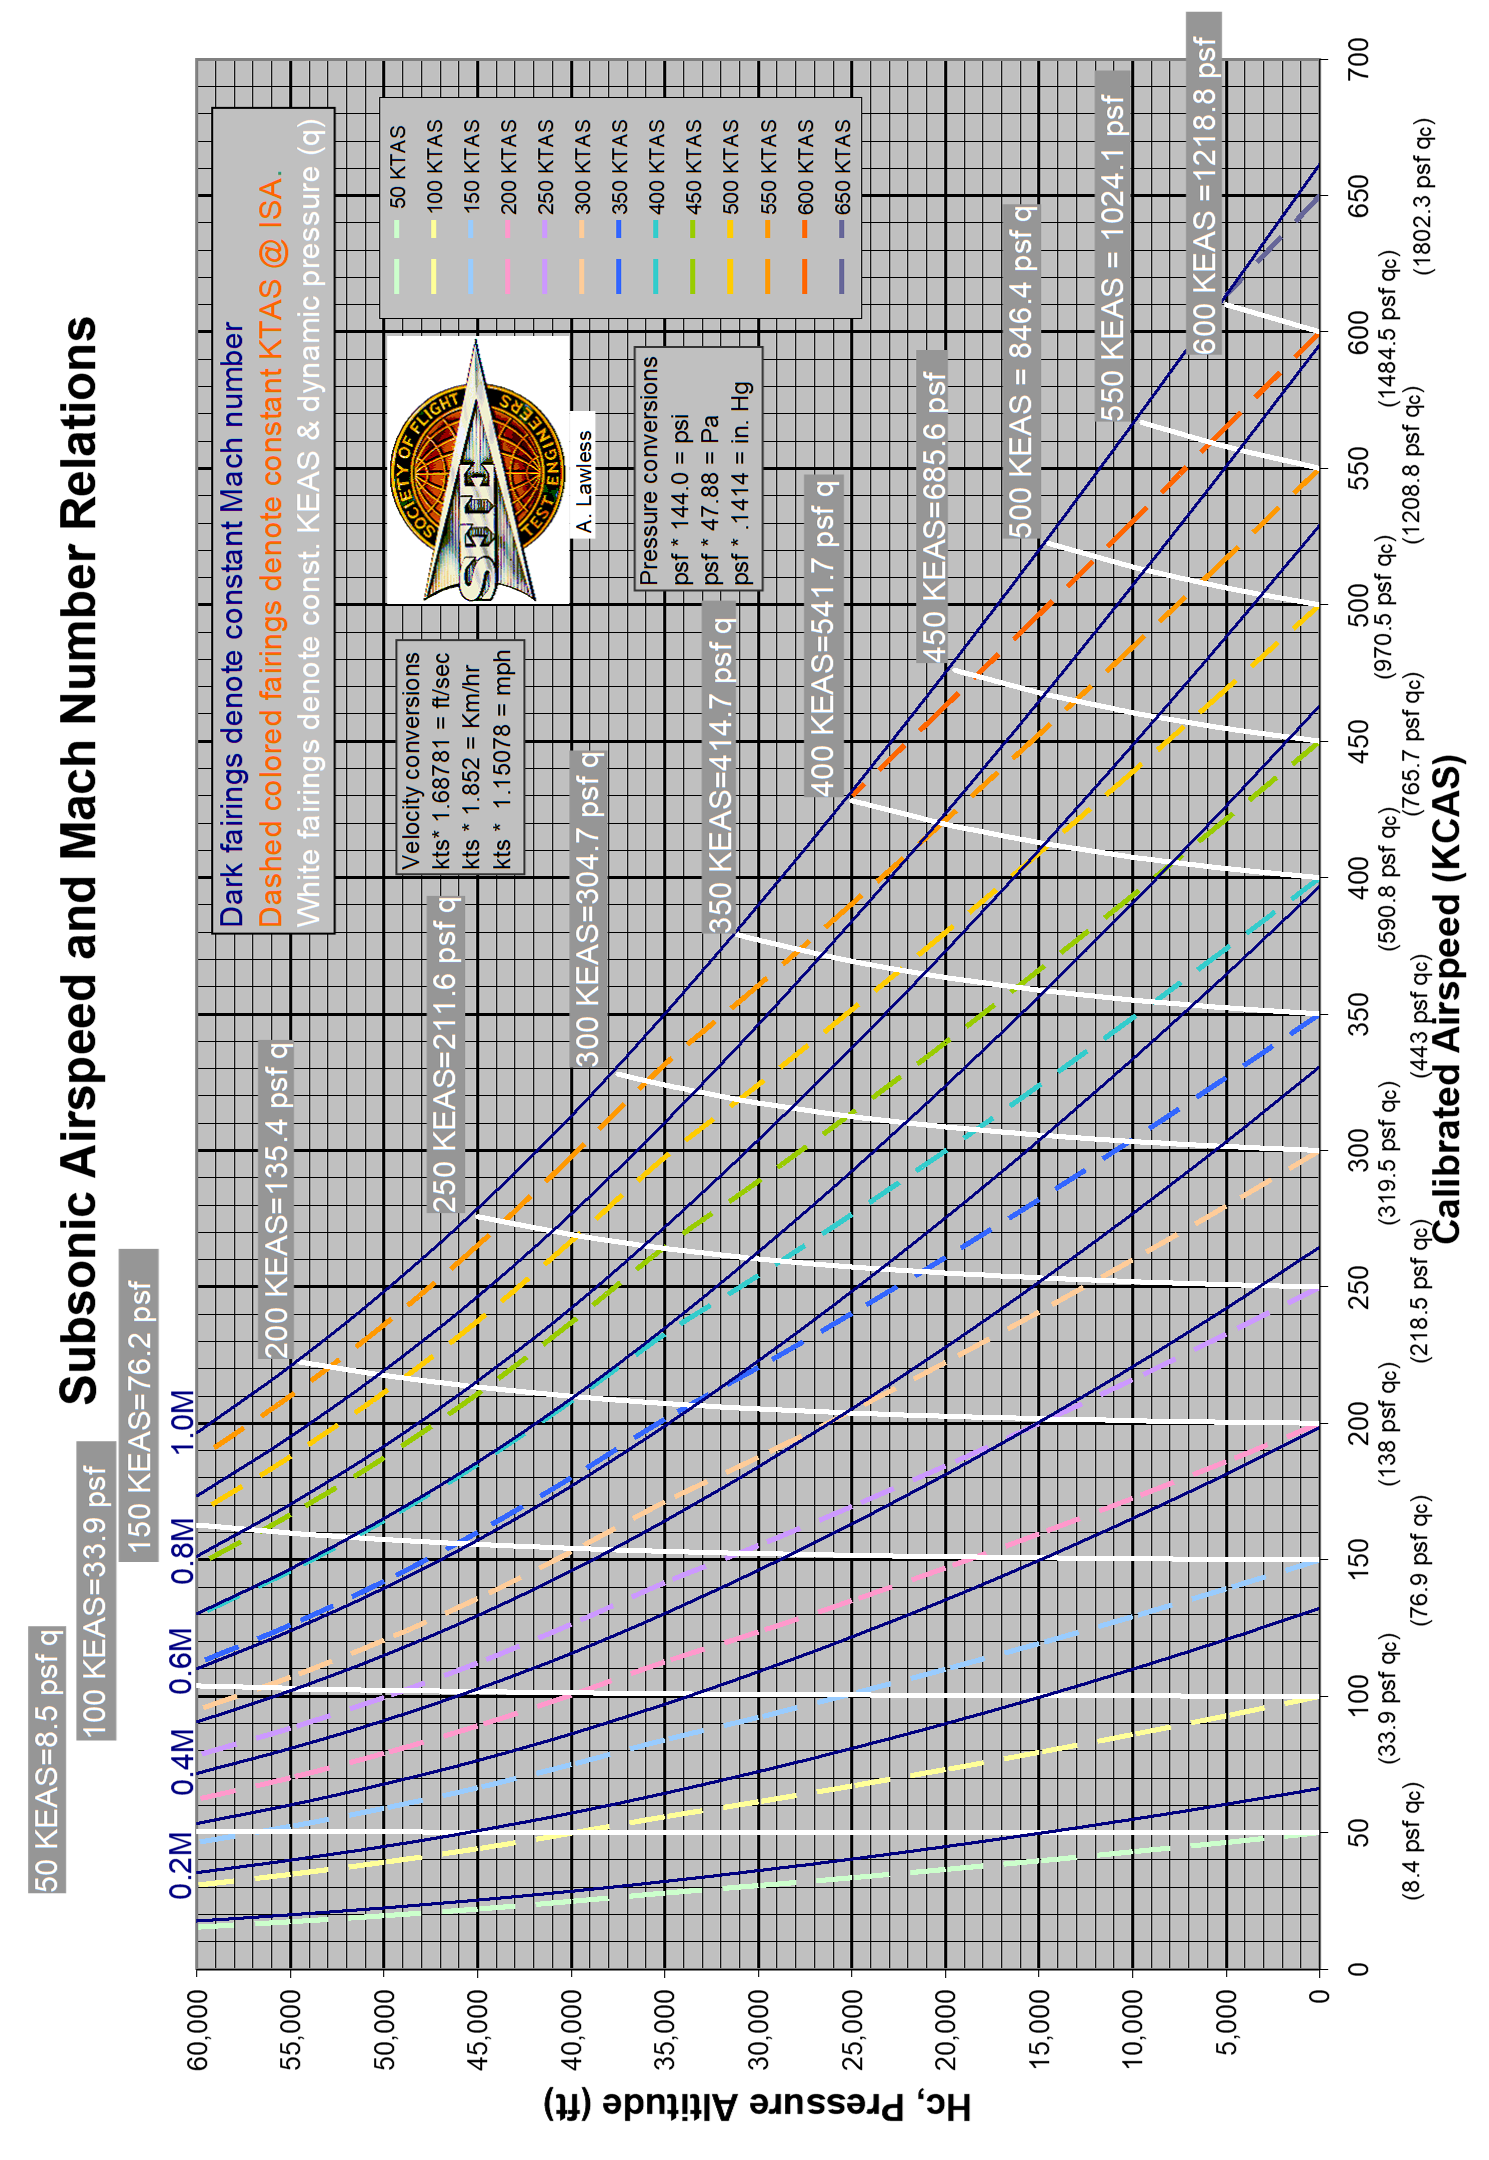
\includegraphics[width=6.42153in,height=9.31667in]{media/04/image54.png}

\hypertarget{effect-of-errors-on-calibrated-airspeed-and-altitude}{%
\section{Effect of Errors on Calibrated Airspeed and Altitude}\label{effect-of-errors-on-calibrated-airspeed-and-altitude}}

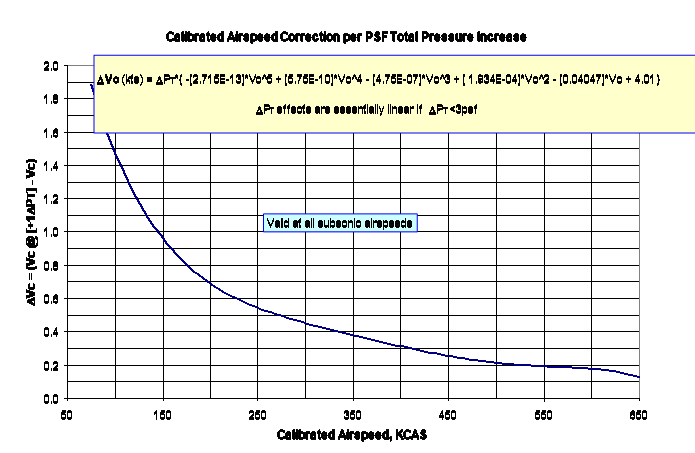
\includegraphics[width=8.6875in,height=5.73819in]{media/04/image55.png}

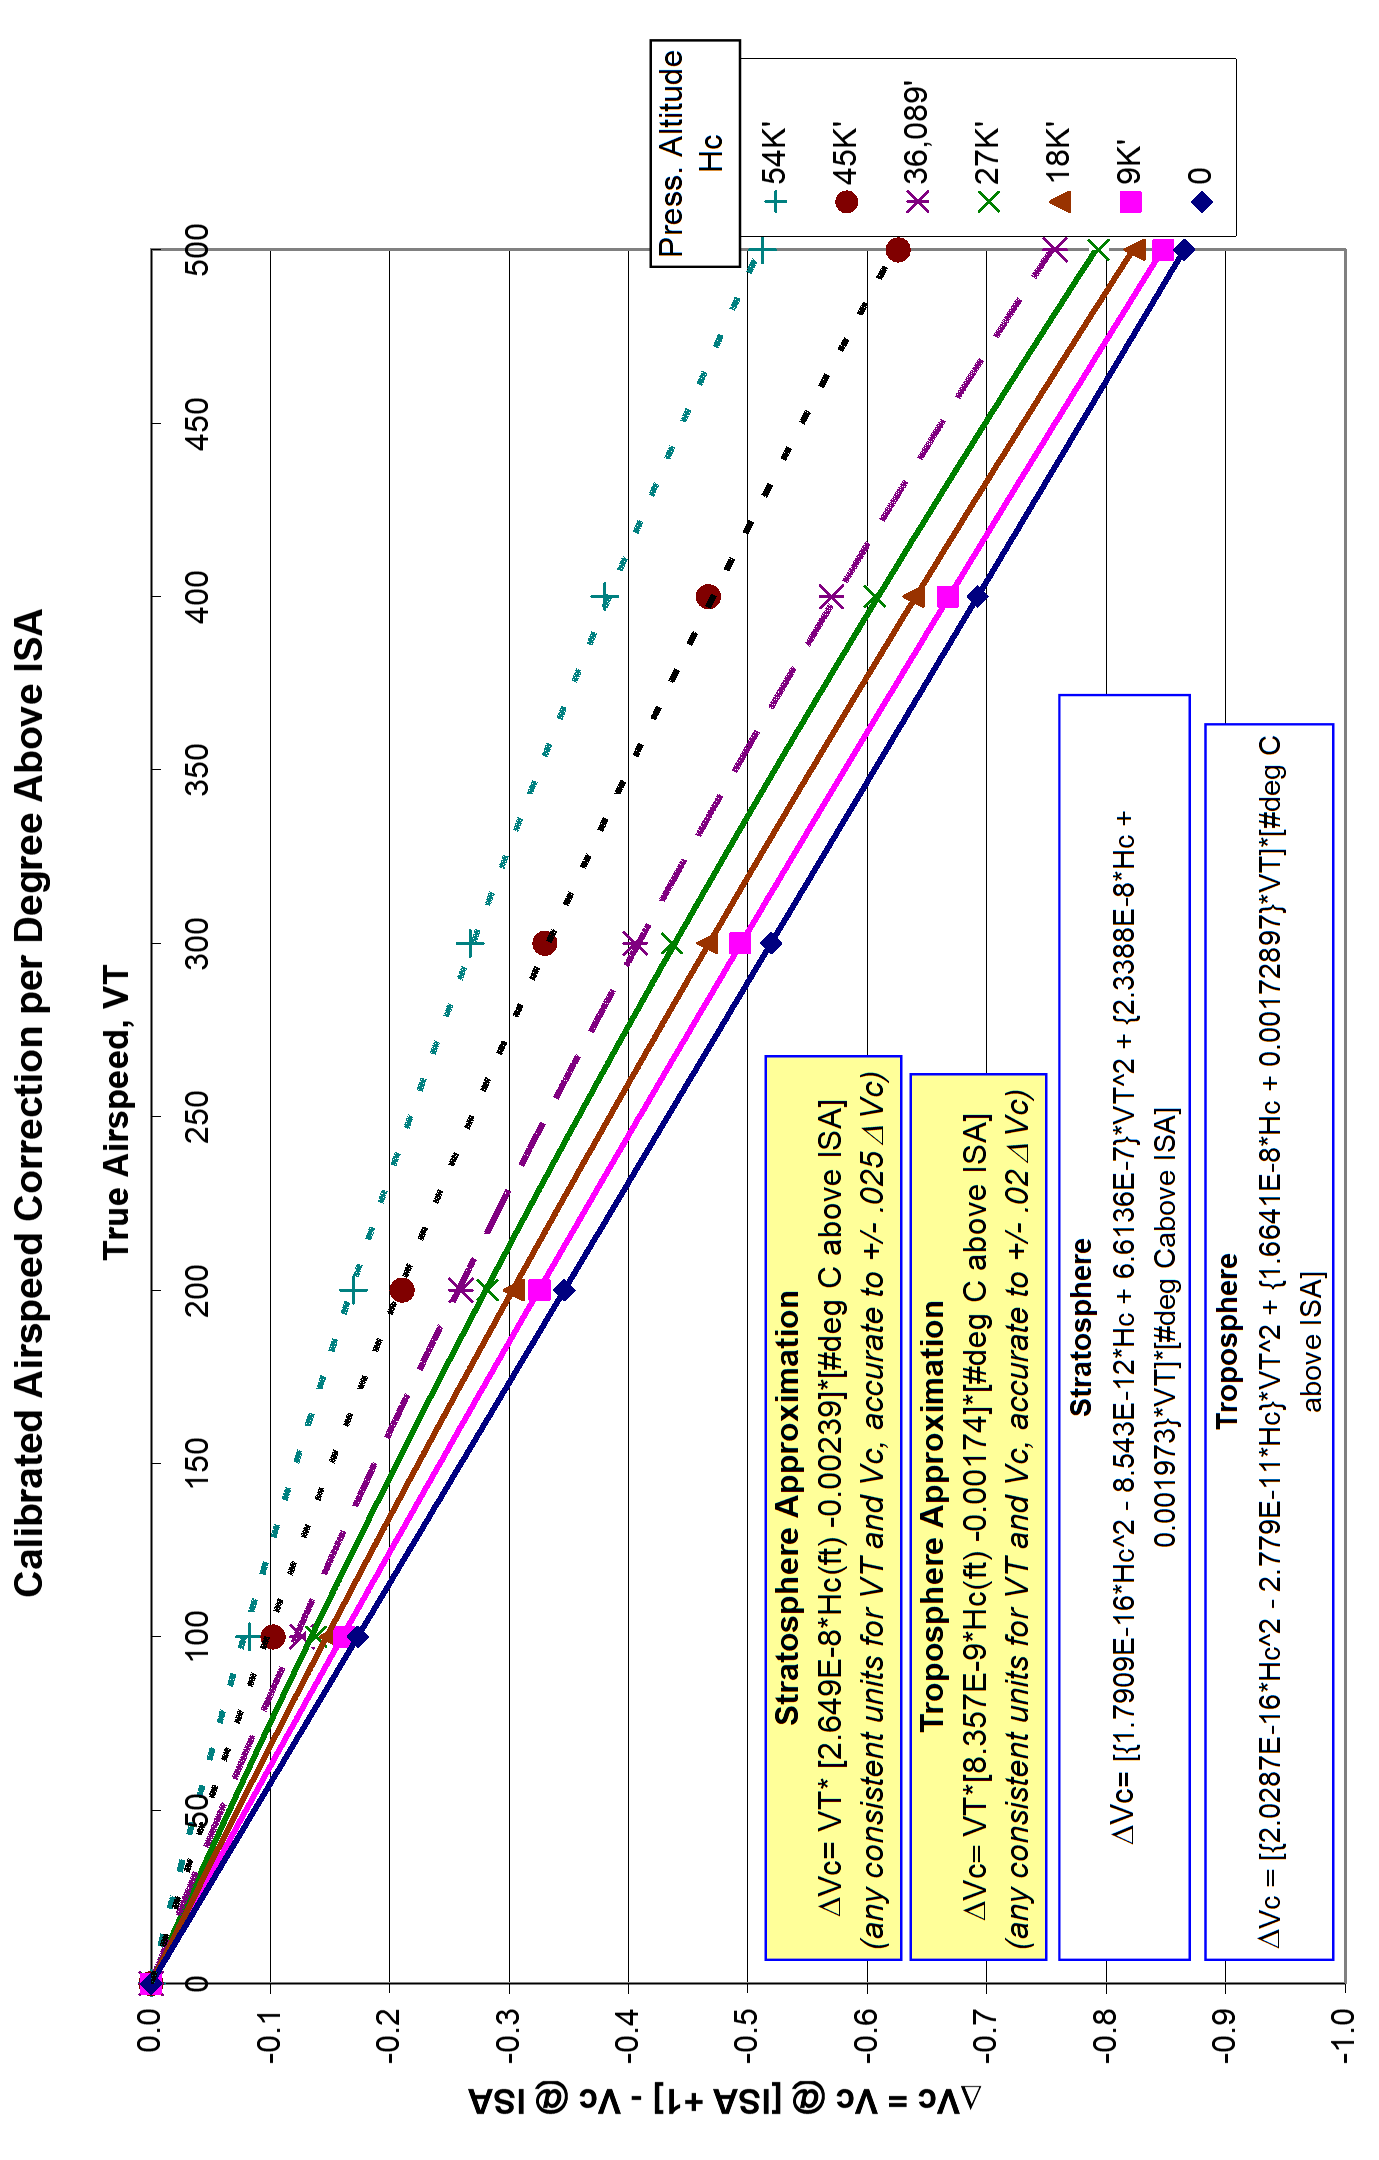
\includegraphics[width=5.74444in,height=9in]{media/04/image56.png}

\includegraphics[width=5.33889in,height=9in]{media/04/image57.png}

\includegraphics[width=6.51111in,height=9in]{media/04/image58.png}

\hypertarget{aerodynamics}{%
\chapter{Aerodynamics}\label{aerodynamics}}

\hypertarget{recurring-terminology}{%
\section*{Recurring Terminology}\label{recurring-terminology}}
\addcontentsline{toc}{section}{Recurring Terminology}

\begin{longtable}[]{@{}ll@{}}
\toprule
\begin{minipage}[b]{0.22\columnwidth}\raggedright
Symbol\strut
\end{minipage} & \begin{minipage}[b]{0.72\columnwidth}\raggedright
Definition\strut
\end{minipage}\tabularnewline
\midrule
\endhead
\begin{minipage}[t]{0.22\columnwidth}\raggedright
\(a\)\strut
\end{minipage} & \begin{minipage}[t]{0.72\columnwidth}\raggedright
slope of lift curve, \(dC_L/d\alpha\)\strut
\end{minipage}\tabularnewline
\begin{minipage}[t]{0.22\columnwidth}\raggedright
\(\mathrm{ac}\)\strut
\end{minipage} & \begin{minipage}[t]{0.72\columnwidth}\raggedright
aerodynamic center, location along the chord where pitching moments about this center do not change with angle of attack (25\% \(\mathrm{MAC}\) for airfoils in subsonic flow, 50\% \(\mathrm{MAC}\) for airfoils in supersonic flow)\strut
\end{minipage}\tabularnewline
\begin{minipage}[t]{0.22\columnwidth}\raggedright
\(\mathrm{AOA}\)\strut
\end{minipage} & \begin{minipage}[t]{0.72\columnwidth}\raggedright
angle of attack\strut
\end{minipage}\tabularnewline
\begin{minipage}[t]{0.22\columnwidth}\raggedright
\(\mathrm{AR}\)\strut
\end{minipage} & \begin{minipage}[t]{0.72\columnwidth}\raggedright
aspect ratio \(= [\text{wing span}]^2 / [\text{reference wing area}] = b^2/S\)\strut
\end{minipage}\tabularnewline
\begin{minipage}[t]{0.22\columnwidth}\raggedright
\(B\)\strut
\end{minipage} & \begin{minipage}[t]{0.72\columnwidth}\raggedright
wing span\strut
\end{minipage}\tabularnewline
\begin{minipage}[t]{0.22\columnwidth}\raggedright
\(b_t\)\strut
\end{minipage} & \begin{minipage}[t]{0.72\columnwidth}\raggedright
horizontal tail span\strut
\end{minipage}\tabularnewline
\begin{minipage}[t]{0.22\columnwidth}\raggedright
\(C\)\strut
\end{minipage} & \begin{minipage}[t]{0.72\columnwidth}\raggedright
coefficient, a non-dimensional representation of an aerodynamic property\strut
\end{minipage}\tabularnewline
\begin{minipage}[t]{0.22\columnwidth}\raggedright
\(c\)\strut
\end{minipage} & \begin{minipage}[t]{0.72\columnwidth}\raggedright
wing chord length Camber maximum curvature of an airfoil, measured at maximum distance between chord line and amber line, expressed in \% of \(\mathrm{MAC}\). Camber line theoretical line extending from an airfoil's leading edge to the trailing edge, located halfway between the upper and lower surfaces.\strut
\end{minipage}\tabularnewline
\begin{minipage}[t]{0.22\columnwidth}\raggedright
\(C_D\)\strut
\end{minipage} & \begin{minipage}[t]{0.72\columnwidth}\raggedright
drag coefficient\strut
\end{minipage}\tabularnewline
\begin{minipage}[t]{0.22\columnwidth}\raggedright
\(C_{D_i}\)\strut
\end{minipage} & \begin{minipage}[t]{0.72\columnwidth}\raggedright
induced drag coefficient\strut
\end{minipage}\tabularnewline
\begin{minipage}[t]{0.22\columnwidth}\raggedright
\(C_{D_0}\text{, }C_{D_{\mathrm{PE}}}\)\strut
\end{minipage} & \begin{minipage}[t]{0.72\columnwidth}\raggedright
parasitic drag coefficient\strut
\end{minipage}\tabularnewline
\begin{minipage}[t]{0.22\columnwidth}\raggedright
\(c_f\)\strut
\end{minipage} & \begin{minipage}[t]{0.72\columnwidth}\raggedright
friction coefficient\strut
\end{minipage}\tabularnewline
\begin{minipage}[t]{0.22\columnwidth}\raggedright
Chord\strut
\end{minipage} & \begin{minipage}[t]{0.72\columnwidth}\raggedright
straight-line distance from an airfoil's leading edge to its trailing edge\strut
\end{minipage}\tabularnewline
\begin{minipage}[t]{0.22\columnwidth}\raggedright
\(C_L\)\strut
\end{minipage} & \begin{minipage}[t]{0.72\columnwidth}\raggedright
lift coefficient\strut
\end{minipage}\tabularnewline
\begin{minipage}[t]{0.22\columnwidth}\raggedright
\(C_p\)\strut
\end{minipage} & \begin{minipage}[t]{0.72\columnwidth}\raggedright
pressure coefficient = \(\Delta p/q\)\strut
\end{minipage}\tabularnewline
\begin{minipage}[t]{0.22\columnwidth}\raggedright
\(e\)\strut
\end{minipage} & \begin{minipage}[t]{0.72\columnwidth}\raggedright
Oswald efficiency factor\strut
\end{minipage}\tabularnewline
\begin{minipage}[t]{0.22\columnwidth}\raggedright
\(l\)\strut
\end{minipage} & \begin{minipage}[t]{0.72\columnwidth}\raggedright
distance traveled by flow, or characteristic length of surface\strut
\end{minipage}\tabularnewline
\begin{minipage}[t]{0.22\columnwidth}\raggedright
\(M\)\strut
\end{minipage} & \begin{minipage}[t]{0.72\columnwidth}\raggedright
Mach number\strut
\end{minipage}\tabularnewline
\begin{minipage}[t]{0.22\columnwidth}\raggedright
\(\mathrm{MAC}\)\strut
\end{minipage} & \begin{minipage}[t]{0.72\columnwidth}\raggedright
mean aerodynamic chord, chord length of location on wing where total aerodynamic forces can be concentrated.\strut
\end{minipage}\tabularnewline
\begin{minipage}[t]{0.22\columnwidth}\raggedright
\(\mathrm{MGC}\)\strut
\end{minipage} & \begin{minipage}[t]{0.72\columnwidth}\raggedright
mean geometric chord, the average chord length, derived only from a plan form view of a wing (similar to \(\mathrm{MAC}\) if wing has no twist and constant cross section \& thickness-to-chord ratio).\strut
\end{minipage}\tabularnewline
\begin{minipage}[t]{0.22\columnwidth}\raggedright
\(P\)\strut
\end{minipage} & \begin{minipage}[t]{0.72\columnwidth}\raggedright
pressure\strut
\end{minipage}\tabularnewline
\begin{minipage}[t]{0.22\columnwidth}\raggedright
\(P_\text{req'd}\)\strut
\end{minipage} & \begin{minipage}[t]{0.72\columnwidth}\raggedright
power required\strut
\end{minipage}\tabularnewline
\begin{minipage}[t]{0.22\columnwidth}\raggedright
\(q\)\strut
\end{minipage} & \begin{minipage}[t]{0.72\columnwidth}\raggedright
dynamic pressure = \(\frac{1}{2} \rho_a V_T^2 = \frac{1}{2} \rho_0 V_T^2\)\strut
\end{minipage}\tabularnewline
\begin{minipage}[t]{0.22\columnwidth}\raggedright
\(R\)\strut
\end{minipage} & \begin{minipage}[t]{0.72\columnwidth}\raggedright
gas constant\strut
\end{minipage}\tabularnewline
\begin{minipage}[t]{0.22\columnwidth}\raggedright
\(\mathrm{Rn},\mathrm{Re}\)\strut
\end{minipage} & \begin{minipage}[t]{0.72\columnwidth}\raggedright
Reynolds number\strut
\end{minipage}\tabularnewline
\begin{minipage}[t]{0.22\columnwidth}\raggedright
\(S\)\strut
\end{minipage} & \begin{minipage}[t]{0.72\columnwidth}\raggedright
reference wing area, includes extension of wing to fuselage centerline.\strut
\end{minipage}\tabularnewline
\begin{minipage}[t]{0.22\columnwidth}\raggedright
\(S_t\)\strut
\end{minipage} & \begin{minipage}[t]{0.72\columnwidth}\raggedright
horizontal tail surface area\strut
\end{minipage}\tabularnewline
\begin{minipage}[t]{0.22\columnwidth}\raggedright
\(S_W\)\strut
\end{minipage} & \begin{minipage}[t]{0.72\columnwidth}\raggedright
wetted area of surface\strut
\end{minipage}\tabularnewline
\begin{minipage}[t]{0.22\columnwidth}\raggedright
\(T\)\strut
\end{minipage} & \begin{minipage}[t]{0.72\columnwidth}\raggedright
temperature\strut
\end{minipage}\tabularnewline
\begin{minipage}[t]{0.22\columnwidth}\raggedright
\(V\)\strut
\end{minipage} & \begin{minipage}[t]{0.72\columnwidth}\raggedright
true velocity\strut
\end{minipage}\tabularnewline
\begin{minipage}[t]{0.22\columnwidth}\raggedright
\(V_e\)\strut
\end{minipage} & \begin{minipage}[t]{0.72\columnwidth}\raggedright
equivalent velocity\strut
\end{minipage}\tabularnewline
\begin{minipage}[t]{0.22\columnwidth}\raggedright
\(\alpha\)\strut
\end{minipage} & \begin{minipage}[t]{0.72\columnwidth}\raggedright
angle of attack\strut
\end{minipage}\tabularnewline
\begin{minipage}[t]{0.22\columnwidth}\raggedright
\(\alpha_i\)\strut
\end{minipage} & \begin{minipage}[t]{0.72\columnwidth}\raggedright
induced angle of attack\strut
\end{minipage}\tabularnewline
\begin{minipage}[t]{0.22\columnwidth}\raggedright
\(\delta\)\strut
\end{minipage} & \begin{minipage}[t]{0.72\columnwidth}\raggedright
depth of boundary layer, or surface wedge angle\strut
\end{minipage}\tabularnewline
\begin{minipage}[t]{0.22\columnwidth}\raggedright
\(\mu\)\strut
\end{minipage} & \begin{minipage}[t]{0.72\columnwidth}\raggedright
viscosity, or wave angle\strut
\end{minipage}\tabularnewline
\begin{minipage}[t]{0.22\columnwidth}\raggedright
\(\nu\)\strut
\end{minipage} & \begin{minipage}[t]{0.72\columnwidth}\raggedright
flow turning angle\strut
\end{minipage}\tabularnewline
\begin{minipage}[t]{0.22\columnwidth}\raggedright
\(\theta\)\strut
\end{minipage} & \begin{minipage}[t]{0.72\columnwidth}\raggedright
shock wave angle\strut
\end{minipage}\tabularnewline
\begin{minipage}[t]{0.22\columnwidth}\raggedright
\(\rho\)\strut
\end{minipage} & \begin{minipage}[t]{0.72\columnwidth}\raggedright
density\strut
\end{minipage}\tabularnewline
\bottomrule
\end{longtable}

\begin{itemize}
\tightlist
\item
  Perfect Fluid

  \begin{itemize}
  \tightlist
  \item
    incompressible, inelastic, and non-viscous
  \item
    used in flow outside of boundary layers at \(M\) \textless{} .7
  \end{itemize}
\item
  Incompressible, inelastic, viscous

  \begin{itemize}
  \tightlist
  \item
    used for boundary layer studies at \(M\) \textless{} .7
  \end{itemize}
\item
  Compressible, non-viscous, elastic fluid

  \begin{itemize}
  \tightlist
  \item
    used outside boundary layers up to \(M\) = 5
  \end{itemize}
\end{itemize}

\hypertarget{dimensional-analysis-interpretations}{%
\section{Dimensional Analysis Interpretations}\label{dimensional-analysis-interpretations}}

(ref 5.2)

Aerodynamic force = \(F\)

\begin{itemize}
\tightlist
\item
  \(F = f \left( \rho \text{, } \mu, T \text{, } V \text{, shape, orientation, size, roughness, gravity} \right)\)
\item
  For aircraft ignore \(R\), \(K\) \& hypersonic effects
\end{itemize}

\includegraphics[width=5.8in,height=3.481in]{media/05/image1.png}

\begin{itemize}
\tightlist
\item
  Initially assume similar body orientations, shapes \& roughness.
\item
  Dimensional Analysis reveals four non-dimensional (\(\pi\)) parameters:

  \begin{itemize}
  \tightlist
  \item
    Force Coefficient \(\pi_1 = \frac{F}{\rho V^2 l^2}\)
  \item
    Reynolds Number \(\pi_2 = \frac{\rho V l}{\mu}\)
  \item
    Mach Number \(\pi_3 = \frac{V}{a}\)
  \item
    Froude Number \(\pi_4 = \frac{V}{\sqrt{lg}}\)
  \end{itemize}
\end{itemize}

A closer look at the force coefficient:

\[C_F = \frac{F}{\rho V^2 l^2} => \frac{F}{\frac{1}{2} \rho V^2 S} \]

where \(\frac{1}{2} \rho_a V_T^2 = \frac{1}{2} \rho_0 V_e^2 = \text{dynamic pressure}\text{, }q\)

Dimensions of reference wing area, \(S\) are the same

\textbf{A feel for \(q\)}

\begin{itemize}
\tightlist
\item
  Kinetic energy of a moving object = \(\frac{1}{2} m V_T^2\)
\item
  Block of moving air kinetic energy = \(\frac{1}{2} \rho \text{ (volume) } V_T^2\)
\item
  Dividing through by volume yields \(\mathrm{KE}\) per volume of moving air = \(\frac{1}{2} \rho V_T^2\)
\item
  ``Dynamic pressure'' or ``\(q\)'' = potential for converting each cubic foot of the airflow's kinetic energy into frontal stagnation pressure
\item
  Feel \(q\) by extending your hand out the window of a moving car
\end{itemize}

\textbf{A feel for coefficients}

\begin{itemize}
\tightlist
\item
  \(C_F = (F/S)/q\) = the ratio between the total force pressure and the flow's dynamic pressure
\item
  Lift is the component of the total force perpendicular to the free stream flow
\item
  Drag is the component along the flow
\item
  Break total into lift and drag coefficients:

  \begin{itemize}
  \tightlist
  \item
    \(C_L = (L/S)/q\)
  \item
    \(C_D = (D/S)/q\)
  \end{itemize}
\item
  Increasing dynamic pressure generates a larger total force, lift and drag
\end{itemize}

\includegraphics[width=\textwidth,height=2.75in]{media/05/image5.png}

\begin{itemize}
\tightlist
\item
  Froude number is not significant in aerodynamic phenomena
\item
  Recall that forces are also a function of angle of attack, shape \& surface roughness, therefore
\end{itemize}

\[C_L,C_D = f \left[ M \text{, } \mathrm{Re} \text{, } \alpha \right] \text{ for a given shape, roughness} \]

\includegraphics[width=5.854in,height=3.863in]{media/05/image7.png}

\emph{Note in the figure above the Reynolds effects are exaggerated}

To compare test day and standard day aircraft or to match wind tunnel \(C_F\) data to actual aircraft; the shape, roughness, \(M\), \(\mathrm{Rn}\) and \(\alpha\) must be equal for both aircraft

\includegraphics[width=8.8in,height=2.25in]{media/05/image9.png}

\[\frac{L_A}{q_A S_A} = C_L = \frac{L_M}{q_M S_M} \]

\hypertarget{general-aerodynamic-relations}{%
\section{General Aerodynamic Relations}\label{general-aerodynamic-relations}}

(refs 5.1, 5.2, 5.10)

Lift \& Drag forces can be described using two approaches:

\begin{enumerate}
\def\labelenumi{\arabic{enumi}.}
\tightlist
\item
  Change in momentum of airstream, \(F=d[mv]/dt\)
\item
  ``Bernoulli'' approach which requires the continuity and conservation of energy equations
\end{enumerate}

\textbf{Continuity Equation}

Fluid Mass in = Fluid Mass out

\[\rho_1 V_1 A_1 = \rho_2 V_2 A_2\]

For subsonic (incompressible) flow \(\rho_1 = \rho_2\)

\[V_1 A_1 = V_2 A_2\]

\textbf{Conservation of Energy} (Bernoulli) \textbf{Equation:}

Potential + Kinetic + Pressure = constant (changes in Potential energy are negligible)

Energy per unit volume is pressure then Dynamic Pressure + Static Pressure = Total Pressure

\[\frac{1}{2}\rho V^2 + p_s = \text{constant} \]
\[\frac{1}{2}\rho V^2 + p_s = p_t \]

\begin{itemize}
\tightlist
\item
  This classic approach only applies in the ``potential flow'' region and not in the boundary layer where energy losses occur
\item
  Pressures around a surface can be calculated or measured from tests and converted into pressure coefficients,
\end{itemize}

\[c_p = \left( p_{\mathrm{local}} - p_{\mathrm{ambient}} \right) / \text{dynamic pressure} = \Delta p/q \]

\begin{itemize}
\tightlist
\item
  \(c_p\) values can be mapped out for all surfaces
\end{itemize}

\includegraphics[width=5.333in,height=4.625in]{media/05/image11.png}

\begin{itemize}
\tightlist
\item
  Summation of all pressures perpendicular to surface yield the pitching moments and the ``\textbf{Resultant Aerodynamic Force}'' which is broken into lift and drag components
\end{itemize}

\includegraphics[width=7.1in,height=3.44in]{media/05/image12.png}

\begin{itemize}
\tightlist
\item
  Lift \& drag forces are referred to the aerodynamic center (\(\mathrm{ac}\)) where the pitching moment is constant for reasonable angles of attack.
\item
  Pitching moments increase with airfoil camber, are zero if symmetric.
\item
  Aerodynamic center is located at 25\% \(\mathrm{MAC}\) for fully subsonic flow and at 50\% \(\mathrm{MAC}\) for fully supersonic flow.
\end{itemize}

\hypertarget{wing-design-effects-on-lift-curve-slope}{%
\section{Wing Design Effects on Lift Curve Slope}\label{wing-design-effects-on-lift-curve-slope}}

(refs 5.1, 5.2, 5.10)

\hypertarget{aspect-ratio-effect}{%
\subsection*{Aspect Ratio Effect}\label{aspect-ratio-effect}}
\addcontentsline{toc}{subsection}{Aspect Ratio Effect}

\begin{itemize}
\tightlist
\item
  Pressure differential at wingtip causes tip vortex
\end{itemize}

\includegraphics[width=4.231in,height=2.375in]{media/05/image13.png}

\includegraphics[width=3.875in,height=2.249in]{media/05/image14.png}

\begin{itemize}
\tightlist
\item
  Vortex creates flow field that reduces \(\mathrm{AOA}\) across wingspan
\end{itemize}

\includegraphics[width=8.8in,height=2.882in]{media/05/image15.png}

\begin{itemize}
\tightlist
\item
  Local \(\mathrm{AOA}\) reductions decrease average lift curve slope
\end{itemize}

\includegraphics[width=5.715in,height=5.024in]{media/05/image16.png}

\emph{2D wing = wind tunnel airfoil extending to walls (infinite aspect ratio).}

\(a_0 = \text{Lift curve slope for an infinite wing}\)

\(a = \text{Lift curve slope for a finite wing}\)

\begin{itemize}
\tightlist
\item
  Above relationship estimated as \(\alpha = \frac{dC_L}{d \alpha} = \frac{a_0}{1+\frac{57.3 a_0}{\pi \mathrm{AR}}}\)
\end{itemize}

\hypertarget{trailing-edge-flap-effects}{%
\subsection*{Trailing Edge Flap Effects}\label{trailing-edge-flap-effects}}
\addcontentsline{toc}{subsection}{Trailing Edge Flap Effects}

\includegraphics[width=7in,height=3.438in]{media/05/image18.png}

\includegraphics[width=5.3in,height=5.3in]{media/05/image19.png}

\hypertarget{leading-edge-flap-effects}{%
\subsection*{Leading Edge Flap Effects}\label{leading-edge-flap-effects}}
\addcontentsline{toc}{subsection}{Leading Edge Flap Effects}

\includegraphics[width=6.385in,height=1.393in]{media/05/image20.png}

\includegraphics[width=5.4in,height=5.29in]{media/05/image21.png}

\hypertarget{boundary-layer-control-effects}{%
\subsection*{Boundary Layer Control Effects}\label{boundary-layer-control-effects}}
\addcontentsline{toc}{subsection}{Boundary Layer Control Effects}

\includegraphics[width=6.294in,height=2.349in]{media/05/image22.png}

\includegraphics[width=4.625in,height=3.738in]{media/05/image23.png}

\hypertarget{elements-of-drag}{%
\section{Elements of Drag}\label{elements-of-drag}}

(refs 5.1, 5.2, 5.10)

\includegraphics[width=8.8in,height=3.5in]{media/05/image24.png}

\begin{itemize}
\tightlist
\item
  Skin friction shear stress is a function of velocity profile at surface
\end{itemize}

\includegraphics[width=7.825in,height=3.25in]{media/05/image25.png}

Shear stress \(\tau_w = \mu \left( \frac{dv}{dy} \right)_{y=0}\)

\begin{itemize}
\tightlist
\item
  Viscosity \(\mu\) increases with temperature (ref 5.9)
\end{itemize}

Sutherland law: \(\mu = \mu_0 \frac{\left( \frac{T}{T_0} \right)^{1.5} \left( T_0 + S \right)}{\left( T + S \right)}\)

Power law: \(\mu = \mu_0 \left( \frac{T}{T_0} \right)^n\)

Where \(T_0 = 273.15 \text{K} = 518.67 \text{R}\)

For air: \(S = 110.4 \text{K} = 199 \text{R} \text{; n=0.67}\)

For air at \(273\) K : \(\mu_0 = 1.717 \times 10^{-5} \left[\text{kg/m s}\right] = 3.59 \times 10^{-7} \left[\text{slug/ft s}\right]\)

Inserting air values (\(T_K=\)Kelvin and \(T_R=\)Rankin) into Sutherland law gives

\[\mu = 1.458 \times 10^{-6} \frac{T_K^{1.5}}{T_K+110.4} \left[\frac{\text{kg}}{\text{s m}}\right] = 2.2 \times 10^{-8} \frac{T_R^{1.5}}{T_R+199} \left[\frac{\text{slug}}{\text{s ft}}\right]\]

\hypertarget{reynolds-number-effects}{%
\subsection{Reynolds Number Effects}\label{reynolds-number-effects}}

(ref 5.10)

\begin{itemize}
\tightlist
\item
  Laminar boundary layers have more gradual change in velocity near surface than turbulent boundary layers.
\item
  High Reynolds numbers help propagate turbulent flow.
\end{itemize}

\includegraphics[width=4.033in,height=1.625in]{media/05/image38.png}

Shearing stress: \(\tau_w = \mu \left(\frac{dv}{dy}\right)_{y=0}\)

Skin friction coefficient: \(C_f = \frac{\tau_w}{\frac{1}{2}\rho_{\infty} V_{\infty}^2} = \frac{\tau_w}{q_{\infty}}\)

Laminar boundary layer: \(\text{Total } C_f = \frac{1.328}{\left(\mathrm{Re}_L \right)^{1/2}}\)

Turbulent boundary layer: \(\text{Total } C_f = \frac{0.455}{\left(\log(\mathrm{Re}_L)\right)^{2.58}} \approx \frac{0.074}{\left(\mathrm{Re}_L\right)^{1/5}}\)

\includegraphics[width=6.699in,height=3.906in]{media/05/image43.png}

\(\mathrm{Re}_L\) based on total length of flat plate

\begin{itemize}
\tightlist
\item
  Depth of boundary layer \((\delta)\) depends on local Reynolds number \((\mathrm{Re}_x)\) and whether the flow is turbulent or laminar.
\end{itemize}

\[\mathrm{Re}_x = \frac{\rho_{\infty} V_{\infty} x}{\mu_{\infty}} \equiv \frac{\text{Inertia Forces}}{\text{Viscous Forces}} \]

\(x =\) distance traveled to point in question

\[\delta_{\mathrm{lam}} = \frac{5.2x}{\sqrt{\mathrm{Re}_x}} \]

\[\delta_{\mathrm{turb}} = \frac{0.37x}{\mathrm{Re}_x^{0.2}} \]

\hypertarget{pressure-drag}{%
\subsection{Pressure Drag}\label{pressure-drag}}

\begin{itemize}
\tightlist
\item
  Ideal frictionless flow has no losses and leads to zero pressure drag
\item
  Real fluids have friction and energy losses along surface
\item
  Energy losses negate total pressure recovery, lead to decreasing total pressure along surface
\end{itemize}

\includegraphics[width=8.8in,height=2.875in]{media/05/image46.png}

\begin{itemize}
\tightlist
\item
  Imbalance of pressures on surfaces causes pressure drag
\end{itemize}

\includegraphics[width=5.5in,height=2.644in]{media/05/image47.png}

\includegraphics[width=5.192in,height=2.75in]{media/05/image48.png}

\begin{itemize}
\tightlist
\item
  Profile streamlining reduces pressure drag
\end{itemize}

\includegraphics[width=8.8in,height=6in]{media/05/image49.png}

\hypertarget{interference-drag}{%
\subsection{Interference Drag}\label{interference-drag}}

\begin{itemize}
\tightlist
\item
  Occurs with multiple surfaces approximately parallel to flow
\item
  Caused by flow's interference with itself or by excessive adverse pressure gradient due to rapidly decreasing vehicle cross section
\item
  Most severe with surfaces at acute angles to each other
\item
  Effects often reduced by fillets around contracting surfaces
\end{itemize}

\includegraphics[width=5.563in,height=2.5in]{media/05/image50.png}

\hypertarget{induced-drag}{%
\subsection{Induced Drag}\label{induced-drag}}

\begin{itemize}
\tightlist
\item
  Wingtip vortex reduces local \(\mathrm{AOA}\) at each station along wing
\item
  Local lift vector is perpendicular to local \(\mathrm{AOA}\)
\item
  Local lift vector is therefore tilted back relative to freestream lift
\item
  Induced drag defined as rearward component of local lift vector
\end{itemize}

\includegraphics[width=8.8in,height=4.25in]{media/05/image51.png}

Induced Drag \[\left(D_i\right)=L\left(\alpha_i\right)\]

For elliptical lift distributions \(\alpha_i = \frac{C_L}{\pi \mathrm{AR}}\)

\[\therefore D_i = L \left(\frac{C_L}{\pi \mathrm{AR}}\right) \text{ but } L=qSC_L \]

\[C_{D_i} = \frac{D_i}{qS} = \frac{C_L^2}{\pi \mathrm{AR}}\]

Oswald efficiency factor, \(e\), accounts for losses in excess of those predicted above (due to uneven downwash and changing interference drag effects).

\[\therefore C_{D_i} = \frac{C_L^2}{\pi \mathrm{AR} e}\]

\hypertarget{aerodynamic-compressibility-relations}{%
\section{Aerodynamic Compressibility Relations}\label{aerodynamic-compressibility-relations}}

(ref 5.8)

\textbf{Prandtl/Glauert Approximation}

Approximates Mach effects on aerodynamics below critical Mach

\[C_{P_{\mathrm{compressible}}} = \frac{1}{\sqrt{1-M^2}}C_{P_{\mathrm{incompressible}}} \]

\textbf{Total vs Ambient Property Relations for Adiabatic Flow}

\[\frac{T_T}{T} = 1 + \frac{\gamma -1}{2}M^2 \text{   Isentropic flow not required}\]
\[\frac{P_T}{P} = \left[1 + \frac{\gamma - 1}{2}M^2 \right]^{\frac{\gamma}{\gamma-1}} \text{   Isentropic (shockless) flow required}\]
\[\frac{\rho_T}{\rho} = \left[1 + \frac{\gamma - 1}{2} M^2 \right]^{\frac{1}{\gamma -1}} \text{   Isentropic flow required} \]

\textbf{Normal Shock Relations}

Assumes isentropic flow on each side of the shock
Assumes flow across shock is adiabatic
Property changes occur in a constant area (throat)

\[\frac{P_2}{P_1} = \frac{1 - \gamma + 2\gamma M_1^2}{1+\gamma} \]
\[\frac{\rho_2}{\rho_1} = \left[\frac{2 + \left(\gamma - 1\right) M_1^2}{\left(\gamma+1\right) M_1^2} \right]^{-1} \]
\[\frac{T_2}{T_1} = \left[\frac{1 - \gamma + 2\gamma M_1^2}{1 + \gamma} \right]\left[\frac{2 + \left(\gamma - 1\right) M_1^2}{\left(1 + \gamma\right) M_1^2} \right] \]
\[M_2^2 = \frac{M_1^2 + \frac{2}{\gamma - 1}}{\frac{2\gamma}{\gamma-1} M_1^2-1} \]

Normal shock summary

\(P_{T_1} > P_{T_2}\)

\(P_{1} < P_{2}\)

\(\rho_{T_1} > \rho_{T_2}\)

\(\rho_{1} < \rho_{2}\)

\(T_{T_1} > T_{T_2}\)

\(T_{1} < T_{2}\)

\(M_1 > M_2\)

\(s_1 < s_2\)

\hypertarget{oblique-shocks}{%
\subsection{Oblique Shocks}\label{oblique-shocks}}

\textbf{Oblique Shock Description}

\includegraphics[width=7.124in,height=4.5in]{media/05/image59.png}

\[\delta = \text{surface turning angle}\]

\[\theta = \text{shock wave angle}\]

\[\text{Subscript 1 denotes upstream conditions}\]

\[\text{Subscript 2 denotes downstream conditions}\]

\textbf{Oblique Shock Relations}

\begin{itemize}
\tightlist
\item
  Calculate \(P_2/P_1\), \(T_2/T_1\), and \(\rho_2/\rho_1\) across oblique shocks by using normal shock equations and substituting \(M_1 \sin\theta\) in place of \(M_1\)
\item
  Calculate total pressure loss across oblique shock as
\end{itemize}

\[\frac{P_{T_2}}{P_{T_1}} = \left[\left[\frac{\gamma - 1}{\gamma + 1} + \frac{2}{{\left(\gamma + 1\right)M_1^2\sin^2\theta}}\right]^{\gamma} \left[\frac{2\gamma}{\gamma+1} M_1^2\sin^2\theta - \frac{\gamma - 1}{\gamma + 1} \right]\right]^{\frac{1}{1 - \gamma}}  \]

\begin{itemize}
\tightlist
\item
  Calculate relation between Mach number and angles as
\end{itemize}

\[M_2^2\sin^2\left(\delta - \theta\right) = \frac{M_1^2 \sin^2\theta + \frac{2}{\gamma-1}}{\frac{2\gamma}{\gamma - 1} M_1^2\sin^2\theta - 1} \]

\textbf{Oblique Shock Turning Angle as a Function of Wave Angle}

\includegraphics[width=8.8in,height=7in]{media/05/image62.png}

\begin{itemize}
\tightlist
\item
  Two \(\theta\) solutions exist for every \(M_1\) \& \(\delta\) combination

  \begin{itemize}
  \tightlist
  \item
    These represent the strong and weak shock solutions
  \item
    Weak shocks normally occur in nature
  \end{itemize}
\item
  There is a minimum Mach number for each turning angle
\item
  The wave angle of a weak shock decreases with increased Mach
\item
  For a given Mach number, \(\theta\) approaches \(\mu\) as \(\delta\) decreases
\end{itemize}

\textbf{Mach Cone Angle}

\includegraphics[width=5.163in,height=4.068in]{media/05/image63.png}

Minimum Wave Angle: \(\mu = \sin^{-1}\left(1/M\right)\)

\hypertarget{supersonic-isentropic-expansion-relation}{%
\subsection{Supersonic Isentropic Expansion Relation}\label{supersonic-isentropic-expansion-relation}}

\includegraphics[width=7.2in,height=5.311in]{media/05/image64.png}

\begin{itemize}
\tightlist
\item
  The wave angle \(\mu\) determines where the lower pressure can be felt and thus where the flow can be accelerated
\item
  As the flow accelerates, a new wave angle forms and the subsequent lower pressure further accelerates the flow
\item
  Results in a series of Mach waves forming a ``fan'' until the flow turns and accelerates so that it is parallel to the new boundary
\end{itemize}

\textbf{Prandtl-Meyer Function}

Shows flow's required turning angle (\(\nu\)) to accelerate from one Mach number to another

\[\nu_M = \sqrt{\frac{\gamma + 1}{\gamma - 1}} \left[\tan^{-1}\sqrt{\frac{\gamma - 1}{\gamma + 1} \left(M^2 - 1\right)} \right] - \tan^{-1}\sqrt{M^2-1} \]

\begin{itemize}
\tightlist
\item
  If upstream Mach \((M_1) = 1\), then \(\nu_1 = 0\), and equation directly relates downstream Mach (\(M_2\)) to surface turning angle (\(\Delta \nu\))
\item
  If \(M_1 > 1\), determine \(M_2\) as follows:

  \begin{itemize}
  \tightlist
  \item
    Calculate upstream ν\textsubscript{1} from above equation
  \item
    Calculate \(\nu_2 = \nu_1 + \Delta \nu\)
  \item
    Reverse above equation to obtain corresponding \(M_2\)
  \end{itemize}
\item
  Above equation is tabulated in NACA TR 1135 and is plotted below
\end{itemize}

\includegraphics[width=8.8in,height=7.5in]{media/05/image66.png}

Example: Flow initially at \(M_1 = 2.0\) accelerates through an expansion corner of 24 deg. Exit Mach number is 3.0

\hypertarget{two-dimensional-supersonic-airfoil-approximations}{%
\subsection{Two-Dimensional Supersonic Airfoil Approximations}\label{two-dimensional-supersonic-airfoil-approximations}}

\begin{itemize}
\tightlist
\item
  Determine surface static pressures by calculating changes through obliques shocks and expansion fans
\end{itemize}

\includegraphics[width=5.075in,height=4.25in]{media/05/image67.png}

\begin{itemize}
\tightlist
\item
  Ackert approximations for thin wings are based on
\end{itemize}

\[C_p = \frac{\Delta P}{q} \cong \pm\frac{2 \delta}{\sqrt{M^2 - 1}} \]

\begin{itemize}
\tightlist
\item
  Double wedge airfoil approximations
\end{itemize}

\includegraphics[width=3.531in,height=1in]{media/05/image69.png}

\[C_L \cong \frac{4 \alpha}{\sqrt{M^2 - 1} }\]

\[C_D \cong \frac{4 \alpha^2}{\sqrt{M^2 - 1}} + \frac{4}{\sqrt{M^2 - 1}}\left(\frac{t}{c}\right)^2\]

\begin{itemize}
\tightlist
\item
  Biconvex wing approximations
\end{itemize}

\includegraphics[width=4.596in,height=1.444in]{media/05/image72.png}

\[C_L \cong \frac{4 \alpha}{\sqrt{M^2 - 1} }\]

\[C_D \cong \frac{4 \alpha^2}{\sqrt{M^2 - 1}} + \frac{5.33}{\sqrt{M^2 - 1}}\left(\frac{t}{c}\right)^2\]

\hypertarget{drag-polars}{%
\section{Drag Polars}\label{drag-polars}}

(ref 5.2)

\hypertarget{drag-polar-construction-and-terminology}{%
\subsection{Drag Polar Construction and Terminology}\label{drag-polar-construction-and-terminology}}

\(C_L = \text{lift coefficient}\)

\(C_D = \text{drag coefficient}\)

\(C_{D_i} = \text{induced drag coefficient}\)

\(C_{D_0} = \text{parasitic drag coefficient}\)

\(\mathrm{AR} = \text{aspect ratio}\)

\(e = \text{Oswald efficiency factor}\)

\(l = \text{length flow has traveled}\)

\(S_{\mathrm{wet}} = \text{wetted area of surface}\)

\(S = \text{reference wing area}\)

\textbf{Simple Drag Polar Equation Limitations}

\begin{itemize}
\tightlist
\item
  No separated flow losses
\item
  Symmetric Camber
\item
  Applies at one Mach, Altitude, \(\mathrm{cg}\)
\end{itemize}

\[C_D = C_{D_0} + \frac{C_L^2}{\pi \mathrm{AR} e} = C_{D_0} + C_{D_i}\]

``Polar'' form of simple drag polar:

\includegraphics[width=4.203in,height=3.513in]{media/05/image73.png}

Linearized form of simple drag polar:

\includegraphics[width=4.272in,height=3.725in]{media/05/image75.png}

\hypertarget{complicating-factors}{%
\subsection{Complicating Factors}\label{complicating-factors}}

\hypertarget{airflow-separation-effects}{%
\subsubsection*{Airflow Separation Effects}\label{airflow-separation-effects}}
\addcontentsline{toc}{subsubsection}{Airflow Separation Effects}

\includegraphics[width=4.75in,height=3.46in]{media/05/image76.png}

Drag Polar Equation Accounting for Flow Separation:

\[C_D = C_{D_{\mathrm{min}}} + \frac{\left(C_L - C_{L_{\mathrm{min}}}\right)^2}{\pi \mathrm{AR} e} +k_2\left(C_L - C_{L_{\mathrm{break}}}\right)\]

\begin{itemize}
\tightlist
\item
  Delete last term if \(C_L < C_{L_{\mathrm{break}}}\)
\item
  Determine \(k_2\) from flight test
\end{itemize}

\hypertarget{reynolds-number-effects-1}{%
\subsubsection*{Reynolds Number Effects}\label{reynolds-number-effects-1}}
\addcontentsline{toc}{subsubsection}{Reynolds Number Effects}

(refs 5.4, 5.11)

\begin{itemize}
\tightlist
\item
  Calculate length \(\mathrm{Re}_L\) and friction coefficient (\(c_f\)) for each surface as
\end{itemize}

\[\mathrm{Re}_L = \frac{\rho Vl}{\mu} = 7.101 \times10^6 \left[\frac{\delta}{\theta^2} \right]\left[\frac{T_K + 110}{398}\right] l \]

\(T_K = \text{Kelvin}\)

\(l = \text{total length, ft}\)

\[c_f = \left[\frac{1.328}{\sqrt{\mathrm{Re}_L}}\right] \left[1 + 0.1305 M^2 \right]^{-0.12} \text{ laminar}\]
or
\[c_f = \left[\frac{0.074}{\left(\mathrm{Re}_L\right)^2} - \frac{1700}{\mathrm{Re}_L}  \right] \text{ transition}\]
or
\[c_f = 0.455\left[\log \mathrm{Re}_L\right]^{-258} \left[1 + 0.144 M^2\right]^{-0.65} \text{ turbulent}\]

\begin{itemize}
\tightlist
\item
  In general, \(c_f\) decreases as \(\mathrm{Rn}\) increases (unless transitioning from laminar to turbulent flow)
\item
  Friction drag \(= c_f q S_{\mathrm{wet}}\) for each component (\(S_{\mathrm{wet}} = \text{wetted area}\))
\item
  Correct from test day to standard day aircraft drag coefficient by summing differences of each component's drag change
\end{itemize}

\[\Delta C_D = \frac{\sum\left(c_{f_s} - c_{f_t} \right) S_{\mathrm{wet}}}{S} \]

\hypertarget{wing-camber-or-incidence-angle-effects}{%
\subsubsection*{Wing Camber or Incidence Angle Effects}\label{wing-camber-or-incidence-angle-effects}}
\addcontentsline{toc}{subsubsection}{Wing Camber or Incidence Angle Effects}

Note slight increase in drag as lift decreases towards zero

\includegraphics[width=5.271in,height=6.875in]{media/05/image80.png}

Linearized drag polar for aircraft with wing camber and/or incidence

\includegraphics[width=6.325in,height=3.274in]{media/05/image81.png}

Revised drag polar equation accounting for wing camber or incidence

\[C_D = C_{D_{\mathrm{min}}} + \frac{\left(C_L - C_{L_{\mathrm{min}}} \right)^2}{\pi \mathrm{AR} e} \]

\begin{itemize}
\tightlist
\item
  Generally not necessary since most flight occurs above \(C_{L_{\mathrm{min}}}\)
\end{itemize}

\hypertarget{mach-number-effects}{%
\subsubsection*{Mach Number Effects}\label{mach-number-effects}}
\addcontentsline{toc}{subsubsection}{Mach Number Effects}

\begin{itemize}
\tightlist
\item
  Aircraft with low parasitic drag coefficients and high fineness ratios pay a relatively small ``wave drag'' penalty.
\end{itemize}

\includegraphics[width=5.851in,height=6.075in]{media/05/image83.png}

\begin{itemize}
\tightlist
\item
  With external stores, same aircraft pays larger Mach penalty
\end{itemize}

\includegraphics[width=6.528in,height=6.229in]{media/05/image84.png}

\hypertarget{propeller-slipstream-effects}{%
\subsubsection*{Propeller Slipstream Effects}\label{propeller-slipstream-effects}}
\addcontentsline{toc}{subsubsection}{Propeller Slipstream Effects}

\begin{itemize}
\tightlist
\item
  a.k.a ``scrubbing'' drag
\item
  Propwash increases flow speed over surface within slipstream
\item
  More drag is created by higher \(q\) and vorticity.
\item
  Function of prop speed and power absorbed (\(C_p\)) or thrust (\(C_T\))
\item
  Problem should be addressed in airframe or propeller models
\end{itemize}

\hypertarget{trim-drag-effects}{%
\subsubsection*{Trim Drag Effects}\label{trim-drag-effects}}
\addcontentsline{toc}{subsubsection}{Trim Drag Effects}

(ref 5.4)

\(e = \text{wing Oswald efficiency factor}\)

\(e_t = \text{tail Oswald efficiency factor}\)

\(b = \text{span}\)

\(b_t = \text{tail span}\)

\(x = \text{wing ac-to-cg distance}\)

\(l = \text{wing ac to tail ac distance}\)

\(S = \text{Area}\)

\includegraphics[width=7.75in,height=2.844in]{media/05/image86.png}

\[C_{D_{\mathrm{trim}}} = \frac{W^2}{\pi q^2 Sb^2e} \left[\frac{2}{lW}\left[x_0 - x_1\right] + \frac{1}{l^2} \left[1 + \frac{S}{S_t} \frac{e}{e_t} \left(\frac{b}{b_t}\right)^2\right] \left[x_0^2 - x_1^2\right] \right]\]

Trim drag change relative to total induced drag:

\[\frac{\Delta C_{D_{\mathrm{trim}}}}{\Delta C_{D_i}} = \frac{x}{l} \left[\frac{x}{l} \left(\frac{b}{b_t}\right)^2 \frac{e}{e_t} - 2 \right] \]

Plot of above equation

\includegraphics[width=6.5in,height=7.507in]{media/05/image89.png}

\hypertarget{drag-polar-analysis}{%
\subsection{Drag Polar Analysis}\label{drag-polar-analysis}}

\[D = \bar{q}SC_D = \bar{q}S \left[C_{D_0} + \frac{C_L^2}{\pi \mathrm{AR} e} \right] = \frac{1}{2}\rho_0 V_e^2 S\left[C_{D_0} + \frac{W^2}{\pi \mathrm{AR} e \left(\frac{1}{2} \rho_0 V_e^2 S \right)^2} \right]\]

\begin{itemize}
\tightlist
\item
  For a given configuration (\(C_{D_0} \text{, } S \text{, } \mathrm{AR} \text{, } e\))
\end{itemize}

\[D = k_1 V_e^2 + k_2 \frac{W^2}{V_e^2} \]

first term = parasitic drag, second term = induced drag

\begin{itemize}
\tightlist
\item
  For any given weight, \(D = f(\text{equivalent airspeed})\) only
\end{itemize}

\includegraphics[width=6.7143in,height=3.875in]{media/05/image95.png}

\begin{itemize}
\tightlist
\item
  Minimum total drag occurs when \(D_{\mathrm{induced}} = D_{\mathrm{parasitic}}\)

  \begin{itemize}
  \tightlist
  \item
    same as speed where \(C_{D_i} = C_{D_0}\)
  \item
    occurs at max \(C_L/C_D\) ratio (same as max \(L/D\) ratio)
  \end{itemize}
\item
  Minimum drag/velocity occurs at min slope of Drag vs V curve

  \begin{itemize}
  \tightlist
  \item
    same as speed where \(3C_{D_i} = C_{D_0}\)
  \item
    occurs at max \(C_L^{1/2}/C_D\) ratio
  \end{itemize}
\end{itemize}

Power required = drag x true airspeed

\[P_{\mathrm{req}} = DV_T = D\frac{V_e}{\sqrt{\sigma}} = k_1\frac{V_e^3}{\sqrt{\sigma}} + k_2\frac{W^2}{\sqrt{\sigma}V_e} \]

Minimum total \(P_{\mathrm{req'd}}\) occurs when \(P_{\mathrm{induced}} = P_{\mathrm{parasitic}}\)

\begin{itemize}
\tightlist
\item
  same as speed where \(C_{D_i} = 3C_{D_0}\)
\item
  occurs at max \(C_L^{3/2}/C_D\) ratio
\end{itemize}

Minimum power/velocity occurs at min slope of \(P_{\mathrm{req'd}}\) vs \(V\) curve

\begin{itemize}
\tightlist
\item
  same as speed where \(C_{D_i} = C_{D_0}\)
\item
  occurs at max \(C_L /C_D\) ratio
\end{itemize}

\textbf{Optimum Aerodynamic Flight Conditions}

\emph{Gliders/ Engine-Out Flight}

\begin{itemize}
\tightlist
\item
  Max range (minimum glide slope) occurs at max \(C_L/C_D\)

  \begin{itemize}
  \tightlist
  \item
    same as condition where \(C_{D_0} = C_{D_i}\) \emph{if} drag polar is parabolic
  \end{itemize}
\item
  Min sink rate (minimum power req'd) occurs at max \(C_L^{3/2} /C_D\) ratio same as condition where \(3C_{D_0} = C_{D_i}\) \emph{if} drag polar is parabolic
\end{itemize}

\emph{Reciprocating Engine Aircraft (assuming constant \(\mathrm{BSFC}\) \& prop \(\eta\))}

\begin{itemize}
\tightlist
\item
  Max range (minimum power/velocity) occurs at max \(C_L/C_D\) ratio

  \begin{itemize}
  \tightlist
  \item
    same as condition where \(C_{D_0} = C_{D_i}\) \emph{if} drag polar is parabolic
  \end{itemize}
\item
  Max endurance (minimum power req'd) occurs at max \(C_L^{3/2} / C_D\)

  \begin{itemize}
  \tightlist
  \item
    same as condition where \(3C_{D_0} = C_{D_i}\) \emph{if} drag polar is parabolic
  \end{itemize}
\end{itemize}

\emph{Turbine Jet Engine Aircraft (assuming constant \(\mathrm{TSFC}\))}

\begin{itemize}
\tightlist
\item
  Max range at constant altitude (minimum drag/velocity)

  \begin{itemize}
  \tightlist
  \item
    occurs at max \(C_L^{1/2} / C_D\) ratio
  \item
    same as condition where \(C_{D_0} = 3C_{D_i}\) \emph{if} drag polar is parabolic
  \end{itemize}
\item
  Best cruise/climb range (maximum \(\left[M \times L/D \right]\) ratio)

  \begin{itemize}
  \tightlist
  \item
    occurs at max \(C_L/C_D^{3/2}\) ratio
  \item
    same as condition where \(C_{D_0} = 2C_{D_i}\) \emph{if} drag polar is parabolic
  \end{itemize}
\item
  Best endurance (minimum drag)

  \begin{itemize}
  \tightlist
  \item
    occurs at max \(C_L/C_D\) ratio
  \item
    same as condition where \(C_{D_0} = C_{D_i}\) \emph{if} drag polar is parabolic
  \end{itemize}
\end{itemize}

\includegraphics[width=5.75in,height=4.174in]{media/05/image97.png}

To calculate optimum speed \(V_2\) for configuration\textsubscript{2} \& weight\textsubscript{2} based on optimum speed \(V_1\) at configuration\textsubscript{1} \& weight\textsubscript{1}

\hypertarget{references-3}{%
\section{References}\label{references-3}}

\begin{longtable}[]{@{}ll@{}}
\toprule
\endhead
\begin{minipage}[t]{0.06\columnwidth}\raggedright
5.1\strut
\end{minipage} & \begin{minipage}[t]{0.88\columnwidth}\raggedright
Roberts, Sean ``Aerodynamics for Flight Testers'' \emph{Chapter 3, Subsonic Aerodynamics}, National Test Pilot School, Mojave, CA, 1999\strut
\end{minipage}\tabularnewline
\begin{minipage}[t]{0.06\columnwidth}\raggedright
5.2\strut
\end{minipage} & \begin{minipage}[t]{0.88\columnwidth}\raggedright
Lawless, Alan R., et al, ``Aerodynamics for Flight Testers'' \emph{Chapter 4, Drag Polars}, National Test Pilot School, Mojave ,CA, 1999\strut
\end{minipage}\tabularnewline
\begin{minipage}[t]{0.06\columnwidth}\raggedright
5.3\strut
\end{minipage} & \begin{minipage}[t]{0.88\columnwidth}\raggedright
Hurt Hugh H., ``Aerodynamics for Naval Aviators,'' University of Southern California, Los Angeles, CA, 1959.\strut
\end{minipage}\tabularnewline
\begin{minipage}[t]{0.06\columnwidth}\raggedright
5.4\strut
\end{minipage} & \begin{minipage}[t]{0.88\columnwidth}\raggedright
McCormick, Barnes W., ``Aerodynamics, Aeronautics, and Flight Mechanics,'' Wilet \&Sons, 1979\strut
\end{minipage}\tabularnewline
\begin{minipage}[t]{0.06\columnwidth}\raggedright
5.5\strut
\end{minipage} & \begin{minipage}[t]{0.88\columnwidth}\raggedright
Stinton, Darryl, ``The Design of the Aeroplane,'' BSP Professional Books, Oxford, 1983\strut
\end{minipage}\tabularnewline
\begin{minipage}[t]{0.06\columnwidth}\raggedright
5.6\strut
\end{minipage} & \begin{minipage}[t]{0.88\columnwidth}\raggedright
Roskam, Jan Dr., ``Airplane Design, Part VI,'' Roskam Aviation and Engineering Corp.~1990\strut
\end{minipage}\tabularnewline
\begin{minipage}[t]{0.06\columnwidth}\raggedright
5.7\strut
\end{minipage} & \begin{minipage}[t]{0.88\columnwidth}\raggedright
Anon, ``Equations, Tables, and Charts for Compressible Flow'' NACA Report 1135, 1953\strut
\end{minipage}\tabularnewline
\begin{minipage}[t]{0.06\columnwidth}\raggedright
5.8\strut
\end{minipage} & \begin{minipage}[t]{0.88\columnwidth}\raggedright
Lewis, Gregory, ``Aerodynamics for Flight Testers'' \emph{Chapter 6, Supersonic Aerodynamics}, National Test Pilot School, Mojave CA, 1999\strut
\end{minipage}\tabularnewline
\begin{minipage}[t]{0.06\columnwidth}\raggedright
5.9\strut
\end{minipage} & \begin{minipage}[t]{0.88\columnwidth}\raggedright
White, Frank M. ``Fluid Mechanics'' pg 29, McGraw-Hill, 1979, ISBN 0-07-069667-5.\strut
\end{minipage}\tabularnewline
\begin{minipage}[t]{0.06\columnwidth}\raggedright
5.10\strut
\end{minipage} & \begin{minipage}[t]{0.88\columnwidth}\raggedright
Anderson, John D. Jr, ``Introduction to Flight'' pg 142, McGraw-Hill, 1989, ISBN 0-07-001641-0.\strut
\end{minipage}\tabularnewline
\begin{minipage}[t]{0.06\columnwidth}\raggedright
5.11\strut
\end{minipage} & \begin{minipage}[t]{0.88\columnwidth}\raggedright
Twaites, Bryan, Editor, ``Incompressible Aerodynamics: An Account of the steady flow of incompressible Fluid Past Aerofoils, Wings, and Other Bodies,'' Dover Publications, 1960.\strut
\end{minipage}\tabularnewline
\bottomrule
\end{longtable}

\hypertarget{axis-systems-and-transformations}{%
\chapter{Axis Systems and Transformations}\label{axis-systems-and-transformations}}

\hypertarget{earth-axis-systems}{%
\section{Earth Axis Systems}\label{earth-axis-systems}}

(Reference 6.6.1)

Both fixed-earth and moving-earth axis systems keep constant \emph{orientation} with respect to the Earth. The \(z\)-axis point towards the center of the Earth.
\emph{The origin of a fixed-earth system does not move relative to the Earth (such as a ground radar site).
}The origin of a moving-earth system does not move relative to its host (such as an aircraft inertial reference unit).

\includegraphics[width=4.70903in,height=3.83958in]{media/06/image1.png}

\hypertarget{aircraft-axis-systems}{%
\section{Aircraft Axis Systems}\label{aircraft-axis-systems}}

(Reference 6.6.2)

\hypertarget{body-axis-system}{%
\subsection{Body Axis System}\label{body-axis-system}}

The \emph{body axis} system, denoted by a subscript \(b\), originates at the aircraft center of gravity. The positive direction of the \(x_b\)-axis is towards the front. The positive direction of the \(y_b\)-axis is towards the right wing tip, and the positive direction of the \(z_b\)-axis is towards the bottom of the aircraft.

\includegraphics[width=3.65625in,height=3.03125in]{media/06/image2.png}

\hypertarget{stability-axis-system}{%
\subsection{Stability Axis System}\label{stability-axis-system}}

The \emph{stability axis} system is similar to the body axis system except that it is rotated about the \(y\)-axis through the angle of attack \(\alpha\).

\includegraphics[width=4.5in,height=1.625in]{media/06/image4.png}

Forces, velocities or accelerations along the stability axes are related to the body axes as follows.
\begin{align}
x_b =& x_s \cos \alpha − z_s \sin \alpha \\
y_b =& y_s \\
z_b =& z_s \cos \alpha + x_s \sin \alpha
\end{align}

For cases where the z axis is defined positive upward (typical for normal-axis accelerometers), we have the following.
\begin{align}
x_b =& x_s \cos \alpha + z_s \sin \alpha \\
z_b =& z_x \cos \alpha - x_s \sin \alpha
\end{align}

\hypertarget{wind-axis-system}{%
\subsection{Wind Axis System}\label{wind-axis-system}}

The \emph{wind axis} system is similar to the stability axis system except it is rotated about the \(z_s\)-axis through the angle of sideslip, \(\beta\).

The term ``wind'' refers to the fact that the freestream relative wind approaches the aircraft directly along the \(x_w\)-axis. This dictates that the true airspeed also lies along the same axis.

\includegraphics[width=1.69931in,height=2.07014in]{media/06/image5.png}

Forces, velocities, or accelerations along the wind axes are related to the stability axes as follows
\begin{align}
x_s =&x_w \cos \beta - y_w \sin \beta \\
y_s =& y_w \cos \beta + x_w \sin \beta \\
z_s =& z_w
\end{align}

The geometric relations between body, stability and wind axis velocities are defined and illustrated here. In general,
\[ \sin \alpha = \frac{w}{V_T \cos \beta}\] and
\[\sin \beta = \frac{V}{V_T}.\]
If \(\beta\) is small, then \(\sin \alpha = w/V_T\) and \(\beta = V / V_T\). If \(alpha\) is small, then \(\alpha = w/V_T\).

\includegraphics[width=2.45903in,height=2.21875in]{media/06/image6.png}

Most aircraft sideslip vanes do not measure \(\beta\) directly. They measure the flanking angle, which is the projection of the relative wind into the aircraft's \(x-y\) plane. The difference between these two angles increases with angle of attack. Ignoring upwash, boom bending, and body axis rate corrections, calculate true sideslip as a function of vane \(\alpha\) and \(\beta\) as follows:
\[\beta_{\mathrm{true}} = \tan^{-1} (an\beta_{\mathrm{vane}})).\]

\hypertarget{wind-body-axis-transformations}{%
\subsection{Wind-Body Axis Transformations}\label{wind-body-axis-transformations}}

(Reference 6.6.1)

Combining the two previous transformations, we see that forces, velocities, or accelerations along the wind axes are related to the body axes as follows.
\[
\begin{bmatrix}
x_b \\
y_b \\
z_b
\end{bmatrix} = 
\begin{bmatrix}
\cos \alpha & 0 & -\sin \alpha \\
0 & 1 & 0 \\
\sin \alpha & 0 & \cos \alpha
\end{bmatrix}
\begin{bmatrix}
\cos \beta & -\sin \beta & 0 \\
\sin \beta & \cos \beta & 0 \\
0 & 0 & 1
\end{bmatrix}
\begin{bmatrix}
x_w \\
y_w \\
z_w 
\end{bmatrix}
\]

After expansion,
\begin{align}
x_b =& \cos \alpha (x_w \cos \beta - y_w \sin \beta) - z_w \sin \alpha \\
y_b =& x_w \sin \beta + y_w \cos \beta \\
z_b =& \sin \alpha (x_w \cos \beta - y_w \cos \beta) + z_w \cos \alpha 
\end{align}

The inverse transform, converting from the body to the wind axis system is as follows.
\[
\begin{bmatrix}
x_w \\
y_w \\
z_w
\end{bmatrix} = 
\begin{bmatrix}
\cos \beta & \sin \beta & 0 \\
-\sin \beta & \cos \beta & 0 \\
0 & 0 & 1
\end{bmatrix}
\begin{bmatrix}
\cos \alpha & 0 & \sin \alpha \\
0 & 1 & 0 \\
-\sin \alpha & 0 & \cos \alpha
\end{bmatrix}
\begin{bmatrix}
x_b \\
y_b \\
z_b 
\end{bmatrix}
\]

After expansion,
\begin{align}
x_w =& \cos \beta (x_b \cos \alpha + z_b \sin \alpha) + y_b \sin \beta \\
y_w =& -\sin \beta(x_b \cos \alpha + z_b \sin \alpha) + y_b \cos \beta \\
z_w =& -x_b \sin \alpha + z_b \cos \alpha 
\end{align}

Note that these equations apply to the sign convention with z+ down. If sign convention (and instrumentation calibration) use z+ upward, then the above equations become:
\begin{align}
x_w =& \cos \beta (x_b \cos \alpha - z_b \sin \alpha) + y_b \sin \beta \\
y_w =& -\sin \beta(x_b \cos \alpha + z_b \sin \alpha) + y_b \cos \beta \\
z_w =& x_b \sin \alpha + z_b \cos \alpha 
\end{align}

\hypertarget{principle-axes}{%
\subsection{Principle Axes}\label{principle-axes}}

The \emph{principle axes} are those about which the products of inertia are zero. They can be equated to the axis of ``dumbells'' which represent concentrated mass elements. Neglecting aerodynamic and gyroscopic effects, an aircraft rotating about one of its principle axes will not tend to cross-couple into motion about any other axis.

\includegraphics[width=4.5in,height=2.375in]{media/06/image11.png}

\hypertarget{euler-angles}{%
\section{Euler Angles}\label{euler-angles}}

(Reference 6.6.1)

\emph{Euler angles} are expressed as yaw, pitch, and roll. The sequence--first yaw, then pitch, then roll--must be maintained to arrive at the proper orientation angles. The Euler angles are defined as follows:

\begin{description}
\tightlist
\item[Yaw Angle]
\(\psi\) - The angle between the projection of the vehicle \(x_b\)-axis onto the horizontal reference plane and some initial reference position of the Earth \(x\)-axis. Yaw angle equals the vehicle heading only if the initial reference is North.
\item[Pitch Angle]
\(\theta\) - The angle in the vertical plane between \(x_b\) and the horizon.
\item[Bank Angle]
\(\phi\) - The angle measured in the \(y-z\) plane of the body-axis system between the \(y\)-axis and the horizontal reference plane. Also known as the roll angle, it is a measure of the rotation about the \(x\)-axis.
\end{description}

\includegraphics[width=4in,height=4.125in]{media/06/image12.png}

\hypertarget{flight-path-angles}{%
\section{Flight Path Angles}\label{flight-path-angles}}

(Reference 6.6.3)

Just as the Euler angles define the attitude of the aircraft with respect to the Earth, three flight path angles describe the vehicle's \emph{cg} trajectory relative to the Earth, not the air mass.

\begin{description}
\tightlist
\item[Flight path heading angle]
\(\sigma\) - This angle, also known as ground track heading, is the horizontal angle between some reference direction (usually North) and the projection of the velocity vector on the horizontal plane. Positive rotation is clockwise, from North to East.
\item[Flight path elevation angle]
\(\gamma\) - The vertical angle between the flightpath and the horizontal plane. Positive angle is above the horizon. During a descent, this is commonly referred to as \emph{glide path angle}.
\item[Flight path bank angle]
\(\mu\) - The angle between the plane formed by the velocity vector and the lift vector and the vertical plane containing the velocity vector. Positive angle is clockwise about the velocity vector, looking forward.
\end{description}

The first two angles above are easily measured using ground-based radar, onboard GPS, or inertial reference systems. If only \(\alpha, \beta\), andthe Euler angles are available, then we can calculate the flightpath angles, assuming zero wind, as follows.
\begin{align}
\gamma =& \arcsin [(\sin\theta  \cos\alpha - \cos\theta  \cos\phi  \sin\alpha) \cos\beta - \cos\theta  \sin\phi  \sin\beta] \\
\sigma =& \psi + \arcsin \left[\frac{\cos\phi \sin\beta - \sin\phi \sin\alpha \cos\beta}{\cos\gamma} \right]\\
\mu =& \arcsin\left[ \frac{\cos\theta \sin\phi \cos\beta + 
(\sin\theta \cos\alpha -\cos\theta \cos\phi \sin\alpha)}{\cos\gamma}  \right]
\end{align}

Technically, the above equations describe the \emph{velocity vector}, that is, the angles relative to the air mass. If the air mass is moving relative to the Earth, as is usually the case, the above equations \emph{do not} describe the true flight path.

Ignorance of the difference between flight path and velocity vector angles can cause considerable confusion when analyzing data from different sources.

\hypertarget{axis-system-transformations}{%
\section{Axis System Transformations}\label{axis-system-transformations}}

(Reference 6.6.2)

Transformation matrix for converting forces, velocities or accelerations from \emph{earth axis system}, also known as inertial, \([X, Y, Z]\), to body coordinates \([x, y, z]\).
\[
\begin{bmatrix}
x_b \\
y_b \\
z_b
\end{bmatrix} = 
\begin{bmatrix}
1 & 0 & 0 \\
0 & \cos\phi & \sin\phi \\
0 & -\sin\phi & \cos\phi
\end{bmatrix}
\begin{bmatrix}
\cos\theta & 0 & -\sin\theta \\
0 & 1 & 0 \\
\sin\theta & 0 & \cos\theta
\end{bmatrix}
\begin{bmatrix}
\cos\psi & \sin\psi & 0 \\
-\sin\psi & \cos\psi & 0 \\
0 & 0 & 1
\end{bmatrix}
\begin{bmatrix}
X \\
Y \\
Z 
\end{bmatrix}
\]

This yields
\[
\begin{bmatrix}
x_b \\
y_b \\
z_b
\end{bmatrix} = 
\begin{bmatrix}
\cos\theta \cos\psi & \cos\theta \sin\psi & -\sin\theta \\
-\cos\theta \sin\psi + \sin\phi \sin\theta \cos\psi & \cos\phi \cos\psi + \sin\phi \sin\theta \sin\psi  & \sin\phi \cos\theta \\
\sin\phi \sin\psi + \cos\phi \sin\theta \cos\psi & -\sin\phi \cos\psi + \cos\phi \sin\theta \sin\psi & \cos\phi \cos\theta
\end{bmatrix}
\begin{bmatrix}
X \\
Y \\
Z 
\end{bmatrix}
\]

The inverse of the above transform matrix converts from the body axis to the inertial axis coordinate system.
\[
\begin{bmatrix}
X \\
Y \\
Z
\end{bmatrix} = 
\begin{bmatrix}
\cos\theta \cos\psi & - \cos\phi \sin\psi + \sin\phi \sin\theta \cos\psi & \sin\phi \sin\psi + \cos\phi \sin\theta \cos\psi \\
\cos\theta \sin\psi & \cos\phi \cos\psi + \sin\phi \sin\theta \sin\psi & -\sin\phi \cos\psi + \cos\phi \sin\theta \sin\psi  \\
-\sin\theta & \sin\phi \cos\theta & \cos\phi \cos\theta
\end{bmatrix}
\begin{bmatrix}
x_b \\
y_b \\
z_b 
\end{bmatrix}
\]

\hypertarget{acceleration-transformations}{%
\subsection{Acceleration Transformations}\label{acceleration-transformations}}

First, we convert body-axis angular rates and linear accelerations into total accelerations along the body axes.
\begin{align}
a_x =& \dot{u} + qw - rv \\
a_y =& \dot{v} + ru -pw \\
a_z =& \dot{w} + pv - qu
\end{align}

We also convert the location and rates of mass elements, \(m_1\), into specific angular momentum.
\begin{align}
\frac{H}{m_1} =& \, \bar{r_1} \times [\bar{\omega} \times \bar{r_1}] \\
\left[ \frac{H}{m_1} \right]\hat{i} =& \, p(y^2 + z^2) - q(xy) - r(xz)\\
\left[ \frac{H}{m_1} \right]\hat{j} =& \, q(x^2+z^2) - r(yz) - p(xy)\\
\left[ \frac{H}{m_1} \right] \hat{k} =& \, r(x^2+y^2) - p(xz) - q(yz)
\end{align}

\hypertarget{transformations-between-body-axis-rates-and-euler-angle-rates}{%
\subsection{Transformations between body axis rates and Euler angle rates}\label{transformations-between-body-axis-rates-and-euler-angle-rates}}

\begin{align}
p =& \, \dot{\phi} -\dot{\psi} \sin\theta\\
q =& \, \dot{\theta} \cos\phi + \dot{\psi} \cos{\theta} \sin{\phi}\\
r =& \, \dot{\psi} \cos\theta \cos\phi - \dot{\theta} \sin\phi\\
\dot{\phi} =& \, p + \tan\theta(q \sin\phi + r\cos\phi) \\
\dot{\theta}=& \, q \cos\phi - r\sin\phi\\
\dot{\psi} =& \frac{q \sin\phi + r \cos\phi}{\cos\theta} \, 
\end{align}

\hypertarget{transformations-from-aerodynamic-angles-to-aircraft-stability-axis-angular-rates}{%
\subsection{Transformations from aerodynamic angles to aircraft stability axis angular rates}\label{transformations-from-aerodynamic-angles-to-aircraft-stability-axis-angular-rates}}

Subscripts \(b, s,\) and \(w\) denote the body, stability and wind axis systems.
\begin{align}
p_s =& p_b \cos\alpha + r_b \sin\alpha\, \\
q_s =& \, q_b\\
r_s =& \, r_b \cos\alpha - p_b \sin\alpha
\end{align}

\hypertarget{transformations-from-aerodynamic-angles-to-the-aircraft-wind-axis-angular-rates}{%
\subsection{Transformations from aerodynamic angles to the aircraft wind axis angular rates}\label{transformations-from-aerodynamic-angles-to-the-aircraft-wind-axis-angular-rates}}

Subscripts \(b, s,\) and \(w\) denote the body, stability and wind axis systems.
\begin{align}
p_w =& p_s \cos\beta + q_s \sin\beta\, \\
q_w =& \, q_s \cos\beta - p_s\sin\beta\\
r_w =& \, r_s
\end{align}

\hypertarget{transformations-from-euler-angles-to-aircraft-body-axis-angular-rates}{%
\subsection{Transformations from Euler angles to aircraft body axis angular rates}\label{transformations-from-euler-angles-to-aircraft-body-axis-angular-rates}}

(Reference 6.6.3)
\begin{align}
\dot{p_b} =& \, \ddot{\phi} - \ddot{\psi}\sin\theta - \dot{\psi} \, \dot{\theta} \cos\theta  \\
\dot{q_b} =& \, \ddot{\theta} \cos\phi - \dot{\theta} \, \dot{\phi} \sin{\phi} + \ddot{\phi} \cos\theta \sin\phi - \dot{\psi} \, \dot{\theta} \sin\theta \sin\phi + \dot{\psi} \, \dot{phi} \cos\theta \cos\phi \\
\dot{r_b} =& \, \ddot{\psi} \cos\theta \cos\phi - \dot{\psi} \, \dot{\theta} \sin\theta \cos\phi - \dot{\psi} \, \dot{\theta} \cos\theta \sin\phi - \ddot{\theta} \sin\phi - \dot{\theta} \, \dot{\phi} \cos\phi
\end{align}

\hypertarget{transformations-from-aerodynamic-angles-and-body-axis-angular-rates-to-aircraft-stability-axis-angular-rates}{%
\subsection{Transformations from aerodynamic angles and body axis angular rates to aircraft stability axis angular rates}\label{transformations-from-aerodynamic-angles-and-body-axis-angular-rates-to-aircraft-stability-axis-angular-rates}}

\begin{align}
\dot{p_s} =& \, \dot{p_b} \cos\alpha + \dot{\alpha} \, p_b \sin\alpha + \dot{r_b}\sin\alpha + \dot{\alpha} \, r_b \cos\alpha  \\
\dot{q_s} =& \, \dot{q_b} \\
\dot{r_s} =& \, \dot{r_b} \cos\alpha - \dot{\alpha} \, r_b \sin\alpha - \dot{p_b}\sin\alpha - \dot{\alpha} \, p_b \cos\alpha
\end{align}

\hypertarget{transformations-from-aerodynamic-angles-and-aircraft-stability-axis-to-aircraft-wind-axis-angular-rates}{%
\subsection{Transformations from aerodynamic angles and aircraft stability axis to aircraft wind axis angular rates}\label{transformations-from-aerodynamic-angles-and-aircraft-stability-axis-to-aircraft-wind-axis-angular-rates}}

\begin{align}
\dot{p_w} =& \, \dot{p_b} \cos\beta + \dot{\beta} \, p_s \sin\beta + \dot{q_s}\sin\beta + \dot{\beta} \, q_s \cos\beta  \\
\dot{q_w} =& \,  \dot{q_s} \cos\beta - \dot{\beta} \, q_s \sin\beta - \dot{p_s} \sin\beta - \dot{\beta} \, p_s \cos\beta\\
\dot{r_w} =& \, \dot{r_s}
\end{align}

\hypertarget{references-4}{%
\section{References}\label{references-4}}

\begin{longtable}[]{@{}ll@{}}
\toprule
\endhead
\begin{minipage}[t]{0.06\columnwidth}\raggedright
6.6.1\strut
\end{minipage} & \begin{minipage}[t]{0.88\columnwidth}\raggedright
Lawless, Alan R., \emph{Math and Physics for Flight Testers} ``Chapter 7, Axis Systems and Transformations,'' National Test Pilot School, Mojave CA, 1998.\strut
\end{minipage}\tabularnewline
\begin{minipage}[t]{0.06\columnwidth}\raggedright
6.6.2\strut
\end{minipage} & \begin{minipage}[t]{0.88\columnwidth}\raggedright
Anon., \emph{Aircraft Flying Qualities, Chapter 4, Equations of Motion}, USAF TestPilot School notes, AFFTC Edwards AFB CA, March 1991.\strut
\end{minipage}\tabularnewline
\begin{minipage}[t]{0.06\columnwidth}\raggedright
6.6.3\strut
\end{minipage} & \begin{minipage}[t]{0.88\columnwidth}\raggedright
Kalviste, Juri, \emph{Flight Dynamics Reference Handbook}, Northrop Corp.~Aircraft Division, April 1988.\strut
\end{minipage}\tabularnewline
\bottomrule
\end{longtable}

\hypertarget{mass-properties}{%
\chapter{Mass Properties}\label{mass-properties}}

\hypertarget{abbreviations-and-terminology-abbreviations}{%
\section{Abbreviations and Terminology Abbreviations}\label{abbreviations-and-terminology-abbreviations}}

\begin{longtable}[]{@{}lll@{}}
\toprule
\begin{minipage}[b]{0.14\columnwidth}\raggedright
Symbol\strut
\end{minipage} & \begin{minipage}[b]{0.68\columnwidth}\raggedright
Definition\strut
\end{minipage} & \begin{minipage}[b]{0.10\columnwidth}\raggedright
Unit\strut
\end{minipage}\tabularnewline
\midrule
\endhead
\begin{minipage}[t]{0.14\columnwidth}\raggedright
\(\Delta I_{\mathrm{am}}\)\strut
\end{minipage} & \begin{minipage}[t]{0.68\columnwidth}\raggedright
equivalent moment of inertia contribution of the air\strut
\end{minipage} & \begin{minipage}[t]{0.10\columnwidth}\raggedright
{[}slug-ft\textsuperscript{2}{]}\strut
\end{minipage}\tabularnewline
\begin{minipage}[t]{0.14\columnwidth}\raggedright
\(\Delta I_{\mathrm{te}}\)\strut
\end{minipage} & \begin{minipage}[t]{0.68\columnwidth}\raggedright
correction for test equipment mass\strut
\end{minipage} & \begin{minipage}[t]{0.10\columnwidth}\raggedright
{[}slug-ft\textsuperscript{2}{]}\strut
\end{minipage}\tabularnewline
\begin{minipage}[t]{0.14\columnwidth}\raggedright
\(\delta\)\strut
\end{minipage} & \begin{minipage}[t]{0.68\columnwidth}\raggedright
tilt of spring assembly (measured positive if tilted nose-down relative to local horizontal).\strut
\end{minipage} & \begin{minipage}[t]{0.10\columnwidth}\raggedright
\strut
\end{minipage}\tabularnewline
\begin{minipage}[t]{0.14\columnwidth}\raggedright
\(\varepsilon\)\strut
\end{minipage} & \begin{minipage}[t]{0.68\columnwidth}\raggedright
inclination of principle axis (positive if tilted down).\strut
\end{minipage} & \begin{minipage}[t]{0.10\columnwidth}\raggedright
\strut
\end{minipage}\tabularnewline
\begin{minipage}[t]{0.14\columnwidth}\raggedright
\(\omega_d\)\strut
\end{minipage} & \begin{minipage}[t]{0.68\columnwidth}\raggedright
damped frequency of oscillation\strut
\end{minipage} & \begin{minipage}[t]{0.10\columnwidth}\raggedright
{[}rad/sec{]}\strut
\end{minipage}\tabularnewline
\begin{minipage}[t]{0.14\columnwidth}\raggedright
\(\omega_n\)\strut
\end{minipage} & \begin{minipage}[t]{0.68\columnwidth}\raggedright
natural frequency of oscillation\strut
\end{minipage} & \begin{minipage}[t]{0.10\columnwidth}\raggedright
{[}rad/sec{]}\strut
\end{minipage}\tabularnewline
\begin{minipage}[t]{0.14\columnwidth}\raggedright
\(\phi\)\strut
\end{minipage} & \begin{minipage}[t]{0.68\columnwidth}\raggedright
angle between aircraft y-axis and line connecting aircraft \(\mathrm{cg}\) with spring attach points.\strut
\end{minipage} & \begin{minipage}[t]{0.10\columnwidth}\raggedright
\strut
\end{minipage}\tabularnewline
\begin{minipage}[t]{0.14\columnwidth}\raggedright
\(a\)\strut
\end{minipage} & \begin{minipage}[t]{0.68\columnwidth}\raggedright
perpendicular distance from the spring line of action to the oscillation axis\strut
\end{minipage} & \begin{minipage}[t]{0.10\columnwidth}\raggedright
{[}ft{]}\strut
\end{minipage}\tabularnewline
\begin{minipage}[t]{0.14\columnwidth}\raggedright
\(\mathrm{cg}\)\strut
\end{minipage} & \begin{minipage}[t]{0.68\columnwidth}\raggedright
center of gravity\strut
\end{minipage} & \begin{minipage}[t]{0.10\columnwidth}\raggedright
\strut
\end{minipage}\tabularnewline
\begin{minipage}[t]{0.14\columnwidth}\raggedright
\(f\)\strut
\end{minipage} & \begin{minipage}[t]{0.68\columnwidth}\raggedright
measured frequency of oscillation\strut
\end{minipage} & \begin{minipage}[t]{0.10\columnwidth}\raggedright
{[}cycles/sec{]}\strut
\end{minipage}\tabularnewline
\begin{minipage}[t]{0.14\columnwidth}\raggedright
\(g\)\strut
\end{minipage} & \begin{minipage}[t]{0.68\columnwidth}\raggedright
Earth's acceleration due to gravity\strut
\end{minipage} & \begin{minipage}[t]{0.10\columnwidth}\raggedright
\strut
\end{minipage}\tabularnewline
\begin{minipage}[t]{0.14\columnwidth}\raggedright
\(h\)\strut
\end{minipage} & \begin{minipage}[t]{0.68\columnwidth}\raggedright
vertical component of the perpendicular distance from the \(\mathrm{cg}\) to the oscillation axis.\strut
\end{minipage} & \begin{minipage}[t]{0.10\columnwidth}\raggedright
\strut
\end{minipage}\tabularnewline
\begin{minipage}[t]{0.14\columnwidth}\raggedright
\(I_{\mathrm{cg}}\)\strut
\end{minipage} & \begin{minipage}[t]{0.68\columnwidth}\raggedright
moment of inertia any axis passing through the \(\mathrm{cg}\)\strut
\end{minipage} & \begin{minipage}[t]{0.10\columnwidth}\raggedright
\strut
\end{minipage}\tabularnewline
\begin{minipage}[t]{0.14\columnwidth}\raggedright
\(I_{x_b}\)\strut
\end{minipage} & \begin{minipage}[t]{0.68\columnwidth}\raggedright
moment of inertia about aircraft body x-axis\strut
\end{minipage} & \begin{minipage}[t]{0.10\columnwidth}\raggedright
\strut
\end{minipage}\tabularnewline
\begin{minipage}[t]{0.14\columnwidth}\raggedright
\(I_{xz}\)\strut
\end{minipage} & \begin{minipage}[t]{0.68\columnwidth}\raggedright
product of inertia in aircraft body x-z plane\strut
\end{minipage} & \begin{minipage}[t]{0.10\columnwidth}\raggedright
\strut
\end{minipage}\tabularnewline
\begin{minipage}[t]{0.14\columnwidth}\raggedright
\(I_{y_b}\)\strut
\end{minipage} & \begin{minipage}[t]{0.68\columnwidth}\raggedright
moment of inertia about aircraft body y-axis\strut
\end{minipage} & \begin{minipage}[t]{0.10\columnwidth}\raggedright
\strut
\end{minipage}\tabularnewline
\begin{minipage}[t]{0.14\columnwidth}\raggedright
\(I_{z_b}\)\strut
\end{minipage} & \begin{minipage}[t]{0.68\columnwidth}\raggedright
moment of inertia about aircraft body z-axis\strut
\end{minipage} & \begin{minipage}[t]{0.10\columnwidth}\raggedright
\strut
\end{minipage}\tabularnewline
\begin{minipage}[t]{0.14\columnwidth}\raggedright
\(I_o\)\strut
\end{minipage} & \begin{minipage}[t]{0.68\columnwidth}\raggedright
moment of inertia about oscillation axis\strut
\end{minipage} & \begin{minipage}[t]{0.10\columnwidth}\raggedright
\strut
\end{minipage}\tabularnewline
\begin{minipage}[t]{0.14\columnwidth}\raggedright
\(K_{\mathrm{tot}}\)\strut
\end{minipage} & \begin{minipage}[t]{0.68\columnwidth}\raggedright
total radius of gyration (includes effect of offset pivot)\strut
\end{minipage} & \begin{minipage}[t]{0.10\columnwidth}\raggedright
\strut
\end{minipage}\tabularnewline
\begin{minipage}[t]{0.14\columnwidth}\raggedright
\(K_o\)\strut
\end{minipage} & \begin{minipage}[t]{0.68\columnwidth}\raggedright
component of spring stiffness perpendicular to vehicle motion\strut
\end{minipage} & \begin{minipage}[t]{0.10\columnwidth}\raggedright
\strut
\end{minipage}\tabularnewline
\begin{minipage}[t]{0.14\columnwidth}\raggedright
\(k\)\strut
\end{minipage} & \begin{minipage}[t]{0.68\columnwidth}\raggedright
spring constant\strut
\end{minipage} & \begin{minipage}[t]{0.10\columnwidth}\raggedright
{[}lb/ft{]}\strut
\end{minipage}\tabularnewline
\begin{minipage}[t]{0.14\columnwidth}\raggedright
\(L\)\strut
\end{minipage} & \begin{minipage}[t]{0.68\columnwidth}\raggedright
rolling moment\strut
\end{minipage} & \begin{minipage}[t]{0.10\columnwidth}\raggedright
\strut
\end{minipage}\tabularnewline
\begin{minipage}[t]{0.14\columnwidth}\raggedright
\(l_{\mathrm{eff}}\)\strut
\end{minipage} & \begin{minipage}[t]{0.68\columnwidth}\raggedright
effective pendulum length\strut
\end{minipage} & \begin{minipage}[t]{0.10\columnwidth}\raggedright
\strut
\end{minipage}\tabularnewline
\begin{minipage}[t]{0.14\columnwidth}\raggedright
\(m\)\strut
\end{minipage} & \begin{minipage}[t]{0.68\columnwidth}\raggedright
mass\strut
\end{minipage} & \begin{minipage}[t]{0.10\columnwidth}\raggedright
\strut
\end{minipage}\tabularnewline
\begin{minipage}[t]{0.14\columnwidth}\raggedright
\(\mathrm{MAC}\)\strut
\end{minipage} & \begin{minipage}[t]{0.68\columnwidth}\raggedright
mean aerodynamic chord\strut
\end{minipage} & \begin{minipage}[t]{0.10\columnwidth}\raggedright
\strut
\end{minipage}\tabularnewline
\begin{minipage}[t]{0.14\columnwidth}\raggedright
\(\mathrm{METO}\)\strut
\end{minipage} & \begin{minipage}[t]{0.68\columnwidth}\raggedright
maximum power (except for takeoff)\strut
\end{minipage} & \begin{minipage}[t]{0.10\columnwidth}\raggedright
\strut
\end{minipage}\tabularnewline
\begin{minipage}[t]{0.14\columnwidth}\raggedright
\(N\)\strut
\end{minipage} & \begin{minipage}[t]{0.68\columnwidth}\raggedright
yawing moment\strut
\end{minipage} & \begin{minipage}[t]{0.10\columnwidth}\raggedright
\strut
\end{minipage}\tabularnewline
\begin{minipage}[t]{0.14\columnwidth}\raggedright
\(p\)\strut
\end{minipage} & \begin{minipage}[t]{0.68\columnwidth}\raggedright
roll rate\strut
\end{minipage} & \begin{minipage}[t]{0.10\columnwidth}\raggedright
\strut
\end{minipage}\tabularnewline
\begin{minipage}[t]{0.14\columnwidth}\raggedright
\(r\)\strut
\end{minipage} & \begin{minipage}[t]{0.68\columnwidth}\raggedright
yaw rate\strut
\end{minipage} & \begin{minipage}[t]{0.10\columnwidth}\raggedright
\strut
\end{minipage}\tabularnewline
\begin{minipage}[t]{0.14\columnwidth}\raggedright
\(T\)\strut
\end{minipage} & \begin{minipage}[t]{0.68\columnwidth}\raggedright
period of oscillation\strut
\end{minipage} & \begin{minipage}[t]{0.10\columnwidth}\raggedright
\strut
\end{minipage}\tabularnewline
\bottomrule
\end{longtable}

\hypertarget{terminology}{%
\subsection*{Terminology}\label{terminology}}
\addcontentsline{toc}{subsection}{Terminology}

\begin{longtable}[]{@{}ll@{}}
\toprule
\begin{minipage}[b]{0.11\columnwidth}\raggedright
Term\strut
\end{minipage} & \begin{minipage}[b]{0.83\columnwidth}\raggedright
Definition\strut
\end{minipage}\tabularnewline
\midrule
\endhead
\begin{minipage}[t]{0.11\columnwidth}\raggedright
allowable \(\mathrm{cg}\) range\strut
\end{minipage} & \begin{minipage}[t]{0.83\columnwidth}\raggedright
Documented on Type Certificate Data Sheet. May be different for takeoff vs landing. Forward limit usually determined by control power limitations, aft limit usually determined by stability requirements.\strut
\end{minipage}\tabularnewline
\begin{minipage}[t]{0.11\columnwidth}\raggedright
datum\strut
\end{minipage} & \begin{minipage}[t]{0.83\columnwidth}\raggedright
The manufacturer defined reference plane used for distance calculations.\strut
\end{minipage}\tabularnewline
\begin{minipage}[t]{0.11\columnwidth}\raggedright
empty weight\strut
\end{minipage} & \begin{minipage}[t]{0.83\columnwidth}\raggedright
Basic aircraft weight with only equipment on board. (without crew, passengers, or fuel). This weight may or may not include oil weight, depending on civil certification date.\strut
\end{minipage}\tabularnewline
\begin{minipage}[t]{0.11\columnwidth}\raggedright
empty weight \(\mathrm{cg}\) range\strut
\end{minipage} & \begin{minipage}[t]{0.83\columnwidth}\raggedright
The allowable \(\mathrm{cg}\) locations for an empty aircraft. This is defined by the manufacturer to help assure that a normally loaded aircraft will have an acceptable total \(\mathrm{cg}\) location.\strut
\end{minipage}\tabularnewline
\begin{minipage}[t]{0.11\columnwidth}\raggedright
lateral\strut
\end{minipage} & \begin{minipage}[t]{0.83\columnwidth}\raggedright
Along the aircraft y-axis.\strut
\end{minipage}\tabularnewline
\begin{minipage}[t]{0.11\columnwidth}\raggedright
longitudinal\strut
\end{minipage} & \begin{minipage}[t]{0.83\columnwidth}\raggedright
Along the aircraft x-axis\strut
\end{minipage}\tabularnewline
\begin{minipage}[t]{0.11\columnwidth}\raggedright
maximum weight\strut
\end{minipage} & \begin{minipage}[t]{0.83\columnwidth}\raggedright
Maximum allowable weight. Usually implies takeoff weight, but may apply to landing or in-flight weight. conditions after aerial refueling.\strut
\end{minipage}\tabularnewline
\begin{minipage}[t]{0.11\columnwidth}\raggedright
minimum fuel\strut
\end{minipage} & \begin{minipage}[t]{0.83\columnwidth}\raggedright
A calculated value that represents the minimum amount of fuel any airplane should have while retaining appropriate flight reserves. Calculated as: min fuel {[}lbs{]} = \(0.5 \, \mathrm{METO}\) {[}hp{]}\strut
\end{minipage}\tabularnewline
\begin{minipage}[t]{0.11\columnwidth}\raggedright
moment arm\strut
\end{minipage} & \begin{minipage}[t]{0.83\columnwidth}\raggedright
Distance between datum plane and \(\mathrm{cg}\) of object\strut
\end{minipage}\tabularnewline
\begin{minipage}[t]{0.11\columnwidth}\raggedright
moment\strut
\end{minipage} & \begin{minipage}[t]{0.83\columnwidth}\raggedright
Product of moment arm and force (weight)\strut
\end{minipage}\tabularnewline
\begin{minipage}[t]{0.11\columnwidth}\raggedright
tare\strut
\end{minipage} & \begin{minipage}[t]{0.83\columnwidth}\raggedright
The bias in weight scales due to test equipment weight or due to scale calibration errors\strut
\end{minipage}\tabularnewline
\begin{minipage}[t]{0.11\columnwidth}\raggedright
useful load\strut
\end{minipage} & \begin{minipage}[t]{0.83\columnwidth}\raggedright
Maximum takeoff weight minus empty weight\strut
\end{minipage}\tabularnewline
\begin{minipage}[t]{0.11\columnwidth}\raggedright
weighing point\strut
\end{minipage} & \begin{minipage}[t]{0.83\columnwidth}\raggedright
Location where aircraft is supported during the \(\mathrm{cg}\) measurement.\strut
\end{minipage}\tabularnewline
\bottomrule
\end{longtable}

\hypertarget{longitudinal-lateral-center-of-gravity-measurement}{%
\section{Longitudinal \& Lateral Center of Gravity Measurement}\label{longitudinal-lateral-center-of-gravity-measurement}}

\hypertarget{test-set-up-procedures-for-empty-weight-mathrmcg-determination}{%
\subsection*{\texorpdfstring{Test set-up procedures for empty weight \(\mathrm{cg}\) determination}{Test set-up procedures for empty weight \textbackslash mathrm\{cg\} determination}}\label{test-set-up-procedures-for-empty-weight-mathrmcg-determination}}
\addcontentsline{toc}{subsection}{Test set-up procedures for empty weight \(\mathrm{cg}\) determination}

\begin{enumerate}
\def\labelenumi{\arabic{enumi}.}
\tightlist
\item
  Clean aircraft including any mud or water seepage.
\item
  Ensure all aircraft equipment in place.
\item
  Drain to only residual oil (for older aircraft that include only residual oil as part of empty weight calculations) or fill to full oil (newer aircraft include full oil for calculations).
\item
  Drain to residual fuel only.
\item
  Rig all equipment in a closed building to eliminate wind effects.
\item
  Calibrate scales.
\item
  Record tare (bias in scale readings, may be due to wheel chocks, jack stands, or other test equipment)
\item
  Place aircraft on scales and level according to manufacturer's specifications.
\item
  Measure longitudinal and lateral distances between scale centers and datum. NOTE: distances behind datum are positive, distances ahead of datum are negative.
\item
  Record each scale weight
\end{enumerate}

\hypertarget{calculating-longitudinal-center-of-gravity}{%
\subsection*{Calculating longitudinal center of gravity}\label{calculating-longitudinal-center-of-gravity}}
\addcontentsline{toc}{subsection}{Calculating longitudinal center of gravity}

\begin{enumerate}
\def\labelenumi{\arabic{enumi}.}
\setcounter{enumi}{10}
\tightlist
\item
  Subtract the tare from each scale reading to get the correct weight.
\item
  Multiply each scale's corrected weight by its distance to the datum. This product is the moment for each scale.
\item
  Sum the moments in step 12.
\item
  Sum the corrected weights.
\item
  Divide the total moment by the total weight,step 13/step 14, to obtain the distance from the datum to the \(\mathrm{cg}\). Some aircraft use this distance for all \(\mathrm{cg}\) references (typically presented in inches).
\item
  Other aircraft refer \(\mathrm{cg}\) location to a percent of the mean aerodynamic chord, \(\mathrm{MAC}\). In this case, subtract the distance between the datum and the leading edge of the \(\mathrm{MAC}\) from the distance in step 15.
\item
  Divide the distance in step 16 by the length of the \(\mathrm{MAC}\). This number is the fraction of the \(\mathrm{cg}\) location along the \(\mathrm{MAC}\).
\item
  To present the above fraction in terms of \% \(\mathrm{MAC}\), multiply by 100.
\end{enumerate}

\hypertarget{example-mathrmcg-calculations}{%
\subsubsection*{\texorpdfstring{Example \(\mathrm{cg}\) calculations}{Example \textbackslash mathrm\{cg\} calculations}}\label{example-mathrmcg-calculations}}
\addcontentsline{toc}{subsubsection}{Example \(\mathrm{cg}\) calculations}

\begin{figure}
\centering
\includegraphics[width=3.38889in,height=1.77083in]{media/07/image1.png}
\caption{Example \(\mathrm{cg}\) calculations}
\end{figure}

Scales read:

\begin{itemize}
\tightlist
\item
  \(320\) lbs @ Nose wheel
\item
  \(816\) lbs @ Right main
\item
  \(810\) lbs @ Left main
\end{itemize}

\hypertarget{example-using-datum-at-main-landing-gear}{%
\paragraph*{Example Using Datum at Main Landing Gear}\label{example-using-datum-at-main-landing-gear}}
\addcontentsline{toc}{paragraph}{Example Using Datum at Main Landing Gear}

\begin{longtable}[]{@{}lrrrrr@{}}
\toprule
Item & Weight & \(\times\) & Arm & \(=\) & Moment\tabularnewline
\midrule
\endhead
Right Wheel & \(816\) lbs & \(\times\) & \(0\) in & \(=\) & \(0\) in-lb\tabularnewline
Left Wheel & \(810\) lbs & \(\times\) & \(0\) in & \(=\) & \(0\) in-lb\tabularnewline
Nose Wheel & \(320\) lbs & \(\times\) & \(-75\) in & \(=\) & \(-24\,000\) in-lb\tabularnewline
\textbf{Total} & \textbf{\(1946\) lbs} & & & & \textbf{\(-24\,000\) in-lb}\tabularnewline
\bottomrule
\end{longtable}

\[\frac{-24\,000 \text{ in-lb}}{1946 \text{ lbs}} = 12.33 \text{ in (Forward of Main Wheel Centerline)} \]

\hypertarget{example-using-datum-at-prop-spinner}{%
\paragraph*{Example Using Datum at Prop Spinner}\label{example-using-datum-at-prop-spinner}}
\addcontentsline{toc}{paragraph}{Example Using Datum at Prop Spinner}

\begin{longtable}[]{@{}lrrrrr@{}}
\toprule
Item & Weight & \(\times\) & Arm & \(=\) & Moment\tabularnewline
\midrule
\endhead
Right Wheel & \(816\) lbs & \(\times\) & \(115\) in & \(=\) & \(93\,840\) in-lb\tabularnewline
Left Wheel & \(810\) lbs & \(\times\) & \(115\) in & \(=\) & \(93\,150\) in-lb\tabularnewline
Nose Wheel & \(320\) lbs & \(\times\) & \(40\) in & \(=\) & \(12\,800\) in-lb\tabularnewline
\textbf{Total} & \textbf{\(1946\) lbs} & & & & \textbf{\(199\,790\) in-lb}\tabularnewline
\bottomrule
\end{longtable}

\[\frac{199\,790 \text{ in-lb}}{1946 \text{ lbs}} = 102.67 \text{ in (Aft of Prop Spinner)} \]

\hypertarget{example-lateral-mathrmcg-calculation}{%
\paragraph*{\texorpdfstring{Example Lateral \(\mathrm{cg}\) Calculation}{Example Lateral \textbackslash mathrm\{cg\} Calculation}}\label{example-lateral-mathrmcg-calculation}}
\addcontentsline{toc}{paragraph}{Example Lateral \(\mathrm{cg}\) Calculation}

\begin{longtable}[]{@{}lrrrrr@{}}
\toprule
Item & Weight & \(\times\) & Arm & \(=\) & Moment\tabularnewline
\midrule
\endhead
Right Wheel & \(816\) lbs & \(\times\) & \(+70\) in & \(=\) & \(57\,120\) in-lb\tabularnewline
Left Wheel & \(810\) lbs & \(\times\) & \(-70\) in & \(=\) & \(-56\,700\) in-lb\tabularnewline
Nose Wheel & \(320\) lbs & \(\times\) & \(0\) in & \(=\) & \(0\) in-lb\tabularnewline
\textbf{Total} & \textbf{\(1946\) lbs} & & & & \textbf{\(420\) in-lb}\tabularnewline
\bottomrule
\end{longtable}

\[\frac{420 \text{ in-lb}}{1946 \text{ lbs}} = 0.216 \text{ in (Right of Centerline)} \]

\hypertarget{correcting-empty-weight-mathrmcg-for-changes-in-fuel-passengers-equipment-or-stores.}{%
\subsection*{\texorpdfstring{Correcting empty weight \(\mathrm{cg}\) for changes in fuel, passengers, equipment or stores.}{Correcting empty weight \textbackslash mathrm\{cg\} for changes in fuel, passengers, equipment or stores.}}\label{correcting-empty-weight-mathrmcg-for-changes-in-fuel-passengers-equipment-or-stores.}}
\addcontentsline{toc}{subsection}{Correcting empty weight \(\mathrm{cg}\) for changes in fuel, passengers, equipment or stores.}

\begin{enumerate}
\def\labelenumi{\arabic{enumi}.}
\tightlist
\item
  Note aircraft empty weight \& empty weight \(\mathrm{cg}\). Multiply these values to obtain the empty weight moment.
\item
  Note the weight and moment arm for each item added to or subtracted from the aircraft (items subtracted are listed as negative weights).
\item
  Multiply each item's weight and arm to determine its moment.
\item
  Sum each item's moment in step 3 with the aircraft empty weight moment.
\item
  Sum each item's weight with the aircraft empty weight.
\item
  Calculate the new \(\mathrm{cg}\), step 4/step 5.
\end{enumerate}

\hypertarget{example-mathrmcg-corrections}{%
\subsubsection*{\texorpdfstring{Example \(\mathrm{cg}\) corrections}{Example \textbackslash mathrm\{cg\} corrections}}\label{example-mathrmcg-corrections}}
\addcontentsline{toc}{subsubsection}{Example \(\mathrm{cg}\) corrections}

Given aircraft with empty weight = \(1075\) lbs and \(\mathrm{cg}\) @ \(84\) inches. Add pilot (\(170\) lbs @ \(85.5\)``), fuel ( \(75\) lbs @ \(94\)''), and oil (\(15\) lbs @ \(31.7\)").

\begin{longtable}[]{@{}lrrrrr@{}}
\toprule
Item & Weight & \(\times\) & Arm & \(=\) & Moment\tabularnewline
\midrule
\endhead
Airplane\textsubscript{(empty)} & \(1075\) lbs & \(\times\) & \(84.0\) in & \(=\) & \(90\,300.0\) in-lb\tabularnewline
Pilot & \(170\) lbs & \(\times\) & \(85.5\) in & \(=\) & \(14\,535.0\) in-lb\tabularnewline
Fuel & \(75\) lbs & \(\times\) & \(94.0\) in & \(=\) & \(7050.0\) in-lb\tabularnewline
Oil & \(15\) lbs & \(\times\) & \(31.7\) in & \(=\) & \(475.5\) in-lb\tabularnewline
\textbf{Total} & \textbf{\(1335\) lbs} & & & & \textbf{\(112\,360.5\) in-lb}\tabularnewline
\bottomrule
\end{longtable}

\[\frac{112\,360.5 \text{ in-lb}}{1335 \text{ lbs}} = 84.16 \text{ in} \]

Given aircraft with empty weight = \(1220\) lbs and \(\mathrm{cg}\) @ 25 inches. Add radio (\(15\) lbs @ \(65\)``), and replace \(11\) lb generator with \(14\) lb generator at same \(21.5\)'' location (in front of datum-located on firewall).

\begin{longtable}[]{@{}lrrrrr@{}}
\toprule
Item & Weight & \(\times\) & Arm & \(=\) & Moment\tabularnewline
\midrule
\endhead
Airplane\textsubscript{(empty)} & \(1220\) lbs & \(\times\) & \(25.0\) in & \(=\) & \(30\,500.0\) in-lb\tabularnewline
Pilot & \(15\) lbs & \(\times\) & \(65.0\) in & \(=\) & \(975.0\) in-lb\tabularnewline
Generator\textsubscript{(removed)} & \(-11\) lbs & \(\times\) & \(-21.5\) in & \(=\) & \(236.5\) in-lb\tabularnewline
Generator\textsubscript{(installed)} & \(+14\) lbs & \(\times\) & \(-21.5\) in & \(=\) & \(-294.0\) in-lb\tabularnewline
\textbf{Total} & \textbf{\(1238\) lbs} & & & & \textbf{\(31\,417.5\) in-lb}\tabularnewline
\bottomrule
\end{longtable}

\[\frac{31\,417.5 \text{ in-lb}}{1238 \text{ lbs}} = 25.38 \text{ in} \]

\hypertarget{vertical-center-of-gravity-measurement}{%
\section{Vertical Center of Gravity Measurement}\label{vertical-center-of-gravity-measurement}}

\begin{enumerate}
\def\labelenumi{\arabic{enumi}.}
\tightlist
\item
  Drain or block landing gear struts to keep distances \(G\), \(J\), and \(V\) constant.
\item
  Level the fuselage and measure the weight on the nose wheel (\(F_o\)).
\item
  Tilt the aircraft at various (\(\theta\)) measure nose wheel weight (\(F\)).
\end{enumerate}

~\includegraphics[width=6.5in,height=2.58542in]{media/07/image7.png}

The change in nose wheel force can be written as

\[ F_0 - F = \left[ V + \frac{B G}{C} \right] \left( \frac{W}{C \cot \theta + G}  \right)\]

\begin{enumerate}
\def\labelenumi{\arabic{enumi}.}
\setcounter{enumi}{3}
\tightlist
\item
  Plot (\(F_o-F\)) vs the term in parenthesis.
\item
  Slope of line equals term in brackets.
\item
  Solve for \(V\) after measuring \(B\), \(C\), \(G\), and the slope.

  \begin{itemize}
  \tightlist
  \item
    This method applies to ``gear down'' \(\mathrm{cg}\).
  \item
    For ``gear up'' add the manufacturer's prediction of the \(\mathrm{cg}\) shift to this result.
    ~
    \includegraphics[width=3.17083in,height=2.69792in]{media/07/image9.png}
  \end{itemize}
\end{enumerate}

\hypertarget{moment-product-of-inertia-measurement}{%
\section{Moment \& Product of Inertia Measurement~}\label{moment-product-of-inertia-measurement}}

The moment of inertia about any axis of a body is the summation of the product of every element's mass and distance squared. Moments of inertia represent the resistance to rotational momentum changes.

\includegraphics[width=2.16458in,height=1.28264in]{media/07/image13.png}

\begin{align}
I_{x_b} &\equiv \int \left( y^2 + z^2 \right) dm \\
I_{y_b} &\equiv \int \left( x^2 + z^2 \right) dm \\
I_{z_b} &\equiv \int \left( x^2 + y^2 \right) dm \\
\end{align}

Products of inertia are also calculated about any body axes. They represent the symmetry of mass distribution (comparing opposing quadrants).

\includegraphics[width=1.79236in,height=1.07083in]{media/07/image16.png}

\begin{align}
I_{xy} &= I_{yx} \equiv \int xy dm \\
I_{yz} &= I_{zy} \equiv \int yz dm \\
I_{zx} &= I_{xz} \equiv \int zx dm \\
\end{align}

\begin{itemize}
\tightlist
\item
  Aircraft moments and products of inertia are calculated using body axes as the reference system.
\item
  Careful documentation can yield inertial predictions within about 1-5\% of actual.
\end{itemize}

\includegraphics[width=3.37222in,height=2.33681in]{media/07/image17.png}

\hypertarget{radius-of-gyration}{%
\subsection{Radius of Gyration}\label{radius-of-gyration}}

\begin{itemize}
\tightlist
\item
  Dimensions of all \(I\) terms are {[}slugs-ft\textsuperscript{2}{]}
\item
  Aircraft moments \& products of inertia are generally assumed to be constant.
\item
  For moments of inertia, mathematically replace \(I\) with the product of total mass times some constant with the dimensions of square feet.
\item
  This constant is called the ``radius of gyration'' (\(k\)).
\item
  If all the mass were concentrated at this radius, it would have the same moment of inertia as the actual body.
\end{itemize}

\[ I_x \equiv \int \left( y^2 + z^2 \right) dm = mk^2_{yz} \]

\textbf{Aircraft moment of inertia summary}

\(I_{z_b}\) is always the largest value.

\(I_{y_b} > I_{x_b}\) for fuselage-loaded aircraft.

\(I_{x_b} > I_{y_b}\ \)for wing-loaded aircraft.

\includegraphics[width=4.5in,height=2.375in]{media/07/image19.png}

\begin{itemize}
\tightlist
\item
  Vehicle mass distribution can be represented with concentrated ``dumbbell'' masses.
\item
  The lines connecting the opposing dumbbells are the \textbf{principle axes}.
\item
  When the principle axis lies along some line different from the body axis, the products of inertia are non-zero.
\item
  If the orientation of the principle axes and the moments of inertia about theses axes are known, then the moments of inertia about any other axis system can be calculated.
\end{itemize}

\hypertarget{parallel-axis-theorem-applications}{%
\subsection{Parallel Axis Theorem Applications}\label{parallel-axis-theorem-applications}}

Shows how to \textbf{determine modified moment of inertia} after some component alterations.

Example: Correct original aircraft roll inertia, \(I_{x_b}\), to a modified value that accounts for the addition of wingtip fuel tanks.

\[ I_{x_{b_{\text{mod}}}} = I_{x_{b_{\text{orig}}}} + \Delta I_{x_{\text{comp}}} \]

*~\(\Delta I_{x_{\text{comp}}}\) is composed of two components

\[ \Delta I_{x_{\text{comp}}} = I_{x_{\text{comp}}} + m_{\text{comp}} r^2 \]

\begin{itemize}
\tightlist
\item
  \(I_{x_{\text{comp}}}\) is the moment of inertia of just the new component about an axis which is parallel to the aircraft axis in question (this axis should run through the component's \(\mathrm{cg}\)).
\item
  \(I_{x_{\text{comp}}}\) can be determined analytically by summing the inertias of every mass element throughout the component (documented for simple shapes in various engineering handbooks).
\item
  \(I_{x_{\text{comp}}}\) can be determined experimentally by ``swinging.'' (\protect\hyperlink{swing-method}{Swing Method})
\item
  \(I_{x_{\text{comp}}}\) is usually much smaller than \(m_{\text{comp}} r^2\) and can often be omitted.
\item
  \(m_{\text{comp}}\) is the component's mass
\item
  \(r\) is the distance from the axis in question to the component's \(\mathrm{cg}\).
\end{itemize}

Similarly, the parallel axis theorem shows how to \textbf{determine modified products of inertia} after some component alterations.

\[ I_{xz_{\text{mod}}} = I_{xz_{\text{orig}}} + \left[ I_{xz_{\text{comp}}} + m_{\text{comp}} xz \right] \]

\(x\) and \(z\) are the distances from the component \(\mathrm{cg}\) to the reference axes.

Moments of inertia are calculated about a set of reference axes which all intersect at the reference \(\mathrm{cg}\). In general, however, the actual \(\mathrm{cg}\) does not lie exactly at this reference \(cg\). The parallel axis theorem shows how to \textbf{correct the moment of inertia to the actual \(\mathrm{cg}\) axis}. As an example, the rolling moment of inertia about the actual \(\mathrm{cg}\) ( \(I_{x_{\mathrm{cg}}}\) ) is calculated from the reference \(I_{x_b}\) as follows.

\[ I_{x_{\mathrm{cg}}} = I_{x_b} - m \left[ y^2 + z^2 \right] \]

where

\begin{itemize}
\tightlist
\item
  \(m\) = total mass
\item
  \(y\) = lateral distance between \(\mathrm{cg}\) and aircraft x-axis.
\item
  \(z\) = vertical distance between \(\mathrm{cg}\) and aircraft x-axis.
\end{itemize}

\hypertarget{measuring-roll-inertia-i_x_b-spring-oscillation-method}{%
\subsection{\texorpdfstring{Measuring Roll Inertia, \(I_{x_b}\) (spring oscillation method)}{Measuring Roll Inertia, I\_\{x\_b\} (spring oscillation method)}}\label{measuring-roll-inertia-i_x_b-spring-oscillation-method}}

\begin{enumerate}
\def\labelenumi{\arabic{enumi}.}
\tightlist
\item
  Balance aircraft on prism-like ``knife edges'' that support wooden cradles that conform to aircraft shape.
\item
  Attach springs (tension springs illustrated here) so they are parallel to line \(a\) as shown.
\end{enumerate}

\includegraphics[width=4.47917in,height=1.52847in]{media/07/image24.png}~

\includegraphics[width=4.45278in,height=1.69375in]{media/07/image25.png}~

\begin{enumerate}
\def\labelenumi{\arabic{enumi}.}
\setcounter{enumi}{2}
\tightlist
\item
  Allow aircraft to oscillate freely in roll after a small disturbance.
\item
  Use \textbf{automatic recording} to determine period of oscillations (\(T\)).
\item
  Calculate damped frequency as
\end{enumerate}

\[ \omega_d = \frac{2\pi}{T} \]

\begin{enumerate}
\def\labelenumi{\arabic{enumi}.}
\setcounter{enumi}{5}
\tightlist
\item
  Record peak magnitude of each oscillation.
\item
  Calculate \(\zeta\) using transient peak ratio method (see {[}Motion and Vibration Analysis{]}).
\item
  Calculate natural frequency as
\end{enumerate}

\[ \omega_n = \frac{\omega_d}{\sqrt{1 - \zeta^2}} \]

\begin{enumerate}
\def\labelenumi{\arabic{enumi}.}
\setcounter{enumi}{8}
\tightlist
\item
  Measure the spring's stiffness (\(K_0\))
\item
  Calculate inertia about oscillation axis (\(I_0\)) as
\end{enumerate}

\[ I_o = \frac{K_o}{\omega_n^2} \]

\begin{enumerate}
\def\labelenumi{\arabic{enumi}.}
\setcounter{enumi}{10}
\tightlist
\item
  Use parallel axis theorem to correct \(I_o\) to a parallel axis passing through the \(cg\).
\item
  Springs, cradles and attachments hardware will change the moment of inertia. Sum their total into a combined ``test equipment inertia'' (\Delta\(I_{\mathrm{te}}\)) and subtract this from the above result.
\end{enumerate}

Combining steps 10-12 gives the complete \textbf{moment of inertia equation}

\[ I_{\mathrm{cg}} = \frac{K_o a^2 - mgh}{\omega_n^2} - md^2 - \Delta I_{\mathrm{te}} \]

where \(h\) is the vertical distance between the \(\mathrm{cg}\) and axis of oscillation and \(d\) is the total distance between the \(\mathrm{cg}\) and the axis of oscillation (\(d\) = \(h\) in the illustrated roll inertia test setup).

\textbf{If automatic recording is not available...}

Accomplish steps 1-3 as described for automatic recording case.

\begin{enumerate}
\def\labelenumi{\arabic{enumi}.}
\setcounter{enumi}{3}
\tightlist
\item
  Use a stopwatch to time several oscillations and calculate \(\omega_d\) as before
\item
  Measure the spring's rotational stiffness (\(K_o\))
\item
  Approximate inertia using the damped frequency using
\end{enumerate}

\[ I_o \approx \frac{K_o}{\omega_d^2}  \]

\begin{enumerate}
\def\labelenumi{\arabic{enumi}.}
\setcounter{enumi}{6}
\tightlist
\item
  Use parallel axis theorem to correct \(I_o\) to a parallel axis passing through the \(cg\).
\item
  Correct for effects of test hardware moment of inertia (\(\Delta I_{\mathrm{te}}\)).
\item
  To correct for errors in the \(I_o\) approximation, apply an "additional mass correction" (\(\Delta I_{\mathrm{am}}\)) which equates the flate plate area damping effect to additional inertia. This correction is detailed in ref. 7.5.3.
\end{enumerate}

Combining steps 6-9 gives

\[ I_{\mathrm{cg}} = \frac{K_o a^2 - mgh}{\omega_d^2} - md^2 - \left(\Delta I_{\mathrm{te}} + \Delta I_{\mathrm{am}} \right) \]

Above methods can also be used to determine \(I_{y_b}\) and \(I_{z_b}\)

\hypertarget{measuring-pitch-inertia-i_y_b-spring-oscillation-method}{%
\subsection{\texorpdfstring{Measuring Pitch Inertia, \(I_{y_b}\) (spring oscillation method)}{Measuring Pitch Inertia, I\_\{y\_b\} (spring oscillation method)}}\label{measuring-pitch-inertia-i_y_b-spring-oscillation-method}}

\begin{enumerate}
\def\labelenumi{\arabic{enumi}.}
\tightlist
\item
  Balance aircraft on knife edges as shown.
\item
  Attach spring perpendicular to line \(a\). Only one spring is required since the aircraft \(\mathrm{cg}\) is off-center. Spring must be stiff enough to hold the aircraft in equilibrium as well as provide a restoring moment during oscillations.
\end{enumerate}

\includegraphics[width=4.5in,height=1.66667in]{media/07/image32.png}

\includegraphics[width=4.5in,height=1.58333in]{media/07/image33.png}

Repeat steps 3-12 and apply the moment of inertia equation to determine \(I_{y_b}\)

\[ I_{\mathrm{cg}} = \frac{K_o a^2 - mgh}{\omega_n^2} - md^2 - \Delta I_{\mathrm{te}} \]

or, for an uninstrumented aircraft,

\[ I_{\mathrm{cg}} = \frac{K_o a^2 - mgh}{\omega_d^2} - md^2 - \left(\Delta I_{\mathrm{te}} + \Delta I_{\mathrm{am}} \right) \]

\hypertarget{measuring-yaw-inertia-i_z_b-spring-oscillation-method}{%
\subsection{\texorpdfstring{Measuring Yaw Inertia, \(I_{z_b}\) (spring oscillation method)}{Measuring Yaw Inertia, I\_\{z\_b\} (spring oscillation method)}}\label{measuring-yaw-inertia-i_z_b-spring-oscillation-method}}

\begin{enumerate}
\def\labelenumi{\arabic{enumi}.}
\tightlist
\item
  Suspend aircraft as shown: fuselage reference line parallel with floor, \(z\)-body axis coincides with the oscillation axis (\(h = d = 0\)). For \(I_{z_b}\) test, set spring assembly tilt angle parallel to floor (\(\delta = 0\)).
\end{enumerate}

\includegraphics[width=4.5in,height=2.57292in]{media/07/image36.png}~

\begin{enumerate}
\def\labelenumi{\arabic{enumi}.}
\setcounter{enumi}{1}
\tightlist
\item
  Ideal case is where the wing attach points are in line with the aircraft \(\mathrm{cg}\) as shown. Springs are perpendicular to the AB line and are parallel.
\end{enumerate}

\includegraphics[width=3.83194in,height=3.08333in]{media/07/image37.png}

If not possible to rig wing attach points in line with the \(\mathrm{cg}\), then keep the springs parallel to each other and measure the angle \(\phi\).~~

•~Calculate \(K_o = k \cos{\phi}\), where \(k\) is the actual spring constant

\includegraphics[width=3.15625in,height=3.08333in]{media/07/image38.png}

Repeat steps 3-12 and apply the moment of inertia equation to determine \(I_{z_b}\). Note that distances \(h\) and \(d\) are zero for a properly suspended aircraft.

\[ I_{\mathrm{cg}} = \frac{K_o a^2 - mgh}{\omega_n^2} - md^2 - \Delta I_{\mathrm{te}} \]

or, for an uninstrumented aircraft,

\[ I_{\mathrm{cg}} = \frac{K_o a^2 - mgh}{\omega_d^2} - md^2 - \left(\Delta I_{\mathrm{te}} + \Delta I_{\mathrm{am}} \right) \]

\hypertarget{measuring-axis-of-inclination-and-i_xz}{%
\subsection{\texorpdfstring{Measuring Axis of Inclination and \(I_{xz}\)}{Measuring Axis of Inclination and I\_\{xz\}}}\label{measuring-axis-of-inclination-and-i_xz}}

\begin{itemize}
\tightlist
\item
  Inclination of principle axis (\(\varepsilon\)) is positive if it lies in the \(+xz\) plane as shown.
\item
  \(I_{xz}\) positive if \(\varepsilon\) is positive.
\end{itemize}

\includegraphics[width=4.5in,height=2.67708in]{media/07/image41.png}

\begin{itemize}
\tightlist
\item
  From equations of motion
\end{itemize}

{[}
\begin{align}
L &= I_x \dot{p} - I_{xz} \left( \dot{r} + pq \right) + \left( I_z - I_y \right) qr \text{and} \\
N &= I_z \dot{r} - I_{xz} \left( \dot{p} - qr \right) + \left( I_y - I_x \right) pq \\
\end{align}

\begin{itemize}
\tightlist
\item
  When forcing small motions about only the yaw axis, \(pq\) and \(qr\) are negligible, giving
\end{itemize}

{[}
\begin{align}
L &= I_x \dot{p} - I_{xz} \dot{r} \text{and} \\
N &=  I_z \dot{r} - I_{xz} \dot{p} \\
\end{align}

\begin{itemize}
\tightlist
\item
  If \(\varepsilon\) (and therefore \(I_{xz}\)) is positive, then yawing to the right will generate a left rolling moment.
\item
  If \(\varepsilon\) and \(I_{xz}\) are negative, a right yaw will generate a \emph{right} moment.
\end{itemize}

\begin{enumerate}
\def\labelenumi{\arabic{enumi}.}
\tightlist
\item
  Determine \(I_{xz}\) and \(\varepsilon\) by repeating yaw experiment for different spring angles (\(\delta\)). Use instrumentation to note for each \(\delta\).
\item
  Graphically determine the angle \(\delta_0\) at which the restoring vector produced by the springs completely counteracts the roll motion.
\end{enumerate}

Plot \(\tan{\delta}\) vs \(\frac{\dot{p}}{\dot{r}}\) as shown.

\includegraphics[width=4.5in,height=2.5in]{media/07/image47.png}

\begin{enumerate}
\def\labelenumi{\arabic{enumi}.}
\setcounter{enumi}{2}
\tightlist
\item
  Determine the point where \(\frac{\dot{p}}{\dot{r}}\) equals zero. This occurs at \(\tan{\delta_0}\).
\item
  Calculate the product of inertia using
\end{enumerate}

\[ I_{xz} = I_z \tan{\delta_0} \]

\begin{enumerate}
\def\labelenumi{\arabic{enumi}.}
\setcounter{enumi}{4}
\tightlist
\item
  Calculate the inclination of the principle axis using
\end{enumerate}

\[ \tan{2\varepsilon} = \frac{2I_{xz}}{I_{z_b} - I_{x_b}} \]

Note: Since the \(I_{xz}\) test objective is to interpolate to a condition where \(\frac{\dot{p}}{\dot{r}}\) equals zero, only the ratio is necessary and the absolute magnitudes of the accelerations are not required. In other words, the roll acceleration sensitivity can be increased to allow for easier measurement of the ratio.

\hypertarget{guidelines-for-spring-oscillation-method}{%
\subsection{Guidelines for Spring Oscillation Method}\label{guidelines-for-spring-oscillation-method}}

\begin{itemize}
\tightlist
\item
  Use only small magnitude oscillations.
\item
  Keep size and radius of knife edges as small as practical.
\item
  Springs are typically linear except around zero load. Best results occur if springs are pre-loaded.
\item
  Choose spring stiffness so oscillation frequency will be within instrumentation limits.
\item
  If using a hand recorded stopwatch, best spring stiffness gives about one cycle per second (\(f = 1\)).
\item
  Estimate the desired spring rate using
\end{itemize}

\[ k = \frac{ \left( I_{\mathrm{cg}} + md^2 \right) \left( 2 \pi f \right)^2 + hmg}{a^2} \]

\begin{itemize}
\tightlist
\item
  The purpose of instrumentation is to provide a means for measuring frequency and magnitude. Any of several parameters will be sufficient, including angular displacement, rate or acceleration, or linear acceleration.
\end{itemize}

\hypertarget{swing-method}{%
\subsection{Swing Method}\label{swing-method}}

\begin{enumerate}
\def\labelenumi{\arabic{enumi}.}
\tightlist
\item
  Suspend component as shown.
\end{enumerate}

\includegraphics[width=2.98264in,height=2.15625in]{media/07/image54.png}~

\begin{enumerate}
\def\labelenumi{\arabic{enumi}.}
\setcounter{enumi}{1}
\tightlist
\item
  Measure pendulum length (\(l\)), component mass (\(m\) ), and the period of oscillation (\(T\)).
\end{enumerate}

\begin{itemize}
\tightlist
\item
  The observed period is a function of the effective pendulum length.
\end{itemize}

\[ \omega = \sqrt{\frac{g}{l_{\mathrm{eff}}}} \;\;\;\;\text{and}\;\;\;\; T = \frac{2 \pi}{\omega} = 2 \pi \sqrt{\frac{l_{\mathrm{eff}}}{g}} \;\;\;\;\text{or}\;\;\;\; l_{\mathrm{eff}} = \left( \frac{T}{2 \pi} \right)^2 g \]

\begin{itemize}
\tightlist
\item
  This effective length is the total radius of gyration \(l_{\mathrm{eff}} = K_{\mathrm{tot}}\)
\item
  The total moment of inertia about the pivot point is the product of mass and radius of gyration squared. The parallel axis theorem states that this also is the sum of the component's moment of inertia about its \(\mathrm{cg}\) plus its mass times the distance between the pivot and the component's \(\mathrm{cg}\).
\end{itemize}

\[ I_{\mathrm{eff}} = m K_{\mathrm{tot}}^2 = I_{\mathrm{cg}} + ml^2 \]

\begin{enumerate}
\def\labelenumi{\arabic{enumi}.}
\setcounter{enumi}{2}
\tightlist
\item
  Solving for the component's moment of inertia about its own \(\mathrm{cg}\) gives
\end{enumerate}

\[ I_{\mathrm{cg}} = m K_{\mathrm{tot}}^2 - ml^2 = m \left( K_{\mathrm{tot}}^2 - l^2 \right) = m \left( \left[ \left( \frac{T}{2 \pi} \right)^2 g \right]^2 - l^2 \right) \]

\hypertarget{references-5}{%
\section{References}\label{references-5}}

\begin{longtable}[]{@{}ll@{}}
\toprule
\endhead
\begin{minipage}[t]{0.05\columnwidth}\raggedright
7.5.1\strut
\end{minipage} & \begin{minipage}[t]{0.89\columnwidth}\raggedright
Lawless, Alan R. et al, ``Special Topics and Aircraft Subsystems Flight Testing,'' \emph{Chapter 1, Mass Properties}, National Test Pilot School, Mojave, CA, 1999.\strut
\end{minipage}\tabularnewline
\begin{minipage}[t]{0.05\columnwidth}\raggedright
7.5.2\strut
\end{minipage} & \begin{minipage}[t]{0.89\columnwidth}\raggedright
Bradfield, Edward N., ``Experimental Determination of the Moments of Inertia, Product of Inertia, and Inclination of the Principle Axis of Conventional Aircraft by the Spring Oscillation Method'' FTC-TIM-1001, AFFTC, Edwards AFB, CA, 1971.\strut
\end{minipage}\tabularnewline
\begin{minipage}[t]{0.05\columnwidth}\raggedright
7.5.3\strut
\end{minipage} & \begin{minipage}[t]{0.89\columnwidth}\raggedright
Malvestuto, S. F., et al, ``Formulas for Additional Mass Corrections to the Moments of Inertia of Airplanes'' TN 1187, Langley Memorial Aeronautical Laboratory, Langley Field Virginia, 1947.\strut
\end{minipage}\tabularnewline
\begin{minipage}[t]{0.05\columnwidth}\raggedright
7.5.4\strut
\end{minipage} & \begin{minipage}[t]{0.89\columnwidth}\raggedright
Lawless, Alan R., ``Fixed Wing Flying Qualities Flight Testing'' \emph{Chapter 7, Equations of Motion}, National Test Pilot School Mojave CA, 1998.\strut
\end{minipage}\tabularnewline
\bottomrule
\end{longtable}

\textbf{Additional Reading}

\begin{longtable}[]{@{}ll@{}}
\toprule
\endhead
\begin{minipage}[t]{0.05\columnwidth}\raggedright
7.5.5\strut
\end{minipage} & \begin{minipage}[t]{0.89\columnwidth}\raggedright
Tanner H.L., ``Measurement of the Moments of Inertia of an Airplane by a Simplified Method'' NACA2201, Ames Aeronautical Laboratory, Moffet Field, CA, 1950.\strut
\end{minipage}\tabularnewline
\begin{minipage}[t]{0.05\columnwidth}\raggedright
7.5.6\strut
\end{minipage} & \begin{minipage}[t]{0.89\columnwidth}\raggedright
Woodward, C.R., et al ``Handbook of Instructions for Experimentally Determining the Moments of Inertia of Aircraft by the Spring Oscillation Method'' TB-822-F-2, ASTIA AD97104, Cornell Aeronautical Laboratory, Buffalo, New York, 1955.\strut
\end{minipage}\tabularnewline
\bottomrule
\end{longtable}

\hypertarget{motion-vibration-analysis}{%
\chapter{Motion \& Vibration Analysis}\label{motion-vibration-analysis}}

\hypertarget{recurring-abbreviations}{%
\section{Recurring Abbreviations}\label{recurring-abbreviations}}

\begin{longtable}[]{@{}ll@{}}
\toprule
\endhead
\(C_{\frac{1}{x}}\) & number of cycles to achieve \(\frac{1}{x}\) amplitude\tabularnewline
\(D\) & damping\tabularnewline
\(D_1,D_2\) & peak-to-peak displacement (subsequent)\tabularnewline
\(\mathrm{FV}\) & final value\tabularnewline
\(F(t)\) & forcing function\tabularnewline
\(f\) & frequency, cycles/sec = \(\omega / \left( 2\pi \right)\)\tabularnewline
\(\mathrm{HCAR}\) & half cycle amplitude ratio (i.e., \(x_2/x_1\), \(x_3/x_2\), etc.)\tabularnewline
\(\mathrm{Im}\) & imaginary axis\tabularnewline
\(M\) & mass\tabularnewline
\(\mathrm{MP}\) & peak overshoot\tabularnewline
\(\mathrm{Re}\) & real axis\tabularnewline
\(\mathrm{rms}\) & root mean square\tabularnewline
\(s_1\), \(s_2\) & equation roots of second order\tabularnewline
\(T\) & period = \(1/f\) = \(2\pi/\omega_d\) (seconds)\tabularnewline
\(T_d\) & delay time (i.e., time to 50\% of \(\mathrm{FV}\) )\tabularnewline
\(T_r\) & rise time (i.e., time from 10\% to 90\% of \(\mathrm{FV}\) )\tabularnewline
\(T_p\) & time to peak amplitude\tabularnewline
\(\mathrm{TPR}\) & transient peak ratio\tabularnewline
\(T_s\) & settling time (time to settle within \(x\%\) of \(\mathrm{FV}\) )\tabularnewline
\(T_{\frac{1}{x}}\) & time to achieve \(\frac{1}{x}\) amplitude\tabularnewline
\(x\) & displacement\tabularnewline
\(x_1\), \(x_2\) & peak displacements (subsequent)\tabularnewline
\(v\) & velocity\tabularnewline
\(v_0\) & peak velocity\tabularnewline
\(\varepsilon\) & \(= \zeta \omega_n / \omega_d = \zeta / \sqrt{1 - \zeta^2}\)\tabularnewline
\(\phi\) & phase lag (radians)\tabularnewline
\(\zeta\) & damping coefficient (non-dimensional)\tabularnewline
\(\sigma\) & damping rate \(=\zeta \omega_n = 1/\tau\)\tabularnewline
\(\tau\) & time constant \(=1/\zeta \omega_n\)\tabularnewline
\(\omega\) & frequency, radians/sec\tabularnewline
\(\omega_d\) & damped natural frequency (rad/sec)\tabularnewline
\(\omega_n\) & natural frequency (rad/sec)\tabularnewline
\bottomrule
\end{longtable}

\hypertarget{first-order-motion}{%
\section{First Order Motion}\label{first-order-motion}}

Found in classical aircraft roll and spiral modes. Named first-order because the motions are described by mathematics using the first derivative of a parameter.

\hypertarget{elements-of-first-order-motion}{%
\subsection{Elements of First Order Motion}\label{elements-of-first-order-motion}}

Mechanical analogy contains elements of mass, damping and sometimes a forcing function.

\textbf{Example 1:} Determine the vertical velocity of a diver as she hits the water at \(10\) ft/s (assume constant body position \& neutral buoyancy)

Summing vertical forces gives

{[}
\begin{align}
\sum F_{\mathrm{vert}} : &M \frac{dV}{dt} + DV = 0 \\
&\frac{dV}{V} + \frac{D}{M} dt = 0 \\
&\int{}{} \frac{dV}{V} = -\int{}{} \frac{D}{M} dt
\end{align}

Since \(D\) \& \(M\) are constant

{[}
\begin{align}
\ln V &= -\frac{D}{M} t + C =  -\frac{D}{M} t + \ln c\\
V_c &= c e^{-\frac{D}{M} t} \;\;\text{complementary solution}\\
\end{align}
~
Apply initial condition

{[}
\begin{align}
V(t=0) &= 10 \mathrm{ft/s} \Rightarrow \\
10 &= C \\
V_T &= 10 e^{-\frac{D}{M} t}
\end{align}

Plot response over time

\includegraphics{media/08/image5.png}

Exponential rate of decay described by \(\frac{D}{M}\) ratio

~

\textbf{Example 2:} Diver with \(20\) lb submerged weight releases from zero velocity at top of pool (quiescent condition).

Solve using Laplace analysis methods:

\begin{align}
M\dot{V} + DV &= 20 \;\;\text{step input} \\
M\left[ sV(s) - V(0) \right] + D V(s) &= \frac{20}{s} \\
sV(s) - V(0) + \frac{D}{M} V(s) &= \frac{20}{M} \frac{1}{s} \\
V(s) \left(s + \frac{D}{M} \right) &= \frac{20}{M} \frac{1}{s} + V(0) \\
V(s) &= \frac{ \frac{20}{M} \frac{1}{s} + V(0) }{s + \frac{D}{M} } \\
&= \left\{
          \frac{
                \frac{20}{M}
                }
                {s \left(
                          s + \frac{D}{M}
                        \right)
                } 
  \right\} + \frac{V(0)}{s + \frac{D}{M}} \\
\end{align}

Use partial fraction:

\begin{align}
\frac{ \frac{20}{M} }{s \left( s + \frac{D}{M} \right) } &= \frac{A}{s} + \frac{B}{s + \frac{D}{M}}\\
&= \frac{A \left( s + \frac{D}{M} \right)}{s \left( s + \frac{D}{M} \right) } + \frac{B s}{s \left( s + \frac{D}{M} \right) }\\
&= \frac{A \left( s + \frac{D}{M} \right) + B s}{s \left( s + \frac{D}{M} \right) }\\
\therefore \frac{20}{M} &= A \left( s + \frac{D}{M} \right) + B s
\end{align}\\
{]}

let \(s = -\frac{D}{M}\):

\[\frac{20}{M} = 0 + B \left(-\frac{D}{M}\right) \Rightarrow B = -\frac{20}{D} \]

let \(s = 0\):

\[\frac{20}{M} = A \left( 0 + \frac{D}{M} \right) + 0 \Rightarrow A = \frac{20}{D} \]

\begin{align}
V(s) &= \left\{ \frac{A}{s} + \frac{B}{s + \frac{D}{M}} \right\} + \frac{V(0)}{s + \frac{D}{M}} \\
&= \left\{ \frac{\frac{20}{D}}{s} + \frac{-\frac{20}{D}}{s + \frac{D}{M}} \right\} + \frac{V(0)}{s + \frac{D}{M}} \\
V(t) &= \left\{ \frac{20}{D} -\frac{20}{D}e^{-\frac{D}{M}t} \right\} + V(0)e^{-\frac{D}{M}t} \\
\end{align}

since \(V(0) = 0\) then

\[ V(t) = \frac{20}{D} \left[ 1  -e^{-\frac{D}{M}t} \right] \]

Note that the steady state value, \(V_{\mathrm{ss}} = \frac{20}{D}\), i.e.

\[ V(t) = V_{\mathrm{ss}} \left[1  -e^{-\frac{D}{M}t} \right] \]

This ``force/damping'' ratio is merely a scaling factor for the steady state.

\includegraphics{media/08/image9.png}

Several methods can be used to describe the quickness of convergence toward steady state (e.g., time to \(99.999\%\) of \(V_{\mathrm{ss}}\), time to \(1/2\) \(V_{\mathrm{ss}}\)).

By convention, we use a \(\%\) that directly reflects the exponent.

Establish a time constant \(\tau\) based on \(\frac{D}{M}\).

\[\frac{D}{M} \equiv \frac{1}{\tau} \]

so

\[e^{-\frac{D}{M}t} = e^{-\frac{t}{\tau}}\]

when

\[t = \tau\]

then

\[e^{-\frac{t}{\tau}} = e^{-\frac{\tau}{\tau}} = e^{-1} = 0.36788\]

so, after \(\frac{M}{D}\) seconds have elapsed, \(V = V_{\mathrm{ss}} \left[1 0.36788 \right] = 63.212\% V_{\mathrm{ss}}\)

\(\tau =\) time constant (time for parameter to reach \(~63\%\) of it's steady state value)

\hypertarget{first-order-motion-descriptive-parameters}{%
\subsection{First Order Motion Descriptive Parameters}\label{first-order-motion-descriptive-parameters}}

\[ x(t) = e^{-\zeta \omega_n t} = e^{-\frac{t}{\tau}} \]

\includegraphics{media/08/image12.png}

\begin{longtable}[]{@{}lll@{}}
\toprule
\endhead
when \(t = 0.6931\tau\): & \(x = e^{−0.6931}\) & \(= 0.5\) (time to half amplitude)\tabularnewline
when \(t = \tau\): & \(x = e^{−1}\) & \(= 0.37\)\tabularnewline
when \(t = 3\tau\):~~~~ & \(x = e^{−3}\) & \(= 0.05\)\tabularnewline
when \(t = 4\tau\): & \(x = e^{−4}\) & \(= 0.02\)\tabularnewline
\bottomrule
\end{longtable}

If exponent \(> 0\), then motion is divergent.

\[x(t) = ce^{mt}\]

where \(m > 0\)

\includegraphics{media/08/image15.png}

\(\tau\) again describes the exponential rate of divergence.

By convention, the ``time to double amplitude'' (\(t_2\)) is usually applied as the evaluation metric.

\(x_{t_2} = 2x_0\) where \(x_0 = ce^{m\cdot 0}\)

Therefore

\begin{align}
x_2 &= 2c \\
2c &= ce^{mt_2} \\
2 &= e^{mt_2} \\
\ln 2 &= mt_2 \\
\therefore \text{Time to double amplitude } \frac{0.6931}{m} = t_2 = 0.693\tau \\
\end{align}

\hypertarget{determining-tau-from-step-input-time-history}{%
\subsection{\texorpdfstring{Determining \(\tau\) from Step Input Time History}{Determining \textbackslash tau from Step Input Time History}}\label{determining-tau-from-step-input-time-history}}

\textbf{Method \#1}

\(\tau\) = time to reach \(0.632 x_{\mathrm{ss}}\)

\includegraphics{media/08/image18.png}

\textbf{Method \#2}

\begin{enumerate}
\def\labelenumi{\arabic{enumi}.}
\tightlist
\item
  Define \(x_{\mathrm{ss}}\)
\item
  Measure \(x_1\) at some time \(t_1\)
\item
  Calculate \(x_2 = 0.632 \left( x_{\mathrm{ss}} + 0.58 x_1 \right)\)
\item
  Find \(t_2\) corresponding to \(x_2\)
\item
  \(t_2 - t_1 = \tau\)
\end{enumerate}

\includegraphics{media/08/image21.png}

\textbf{Method \#3}

\begin{enumerate}
\def\labelenumi{\arabic{enumi}.}
\tightlist
\item
  Pick any time \(t_1\).
\item
  Draw tangent at \(t_1\).
\item
  Note \(t_2\) where tangent intercepts \(x_{\mathrm{ss}}\).
\item
  \(\tau = t_2 -t_1\)
\end{enumerate}

\includegraphics{media/08/image22.png}

\textbf{Method \#4}

When \(X_{\mathrm{SS}}\) is unknown use

\[\tau = \frac{\Delta t}{\ln \left( \frac{A_1}{A_2} \right)} \]

\includegraphics{media/08/image24.png}

\textbf{Method \#5}

When \(X_{\mathrm{SS}}\) is known, use

\[\tau = \frac{-\Delta t}{\ln \left[ \frac{X_{\mathrm{SS}} - X_1}{X_{\mathrm{SS}} - X_2} \right]} \]

\textbf{Linearity check:}

Note parameter change between even time increments.

Plot parameter changes vs elapsed time on semi-log scale

\includegraphics{media/08/image26.png}

Slope of line equals \(\tau\)

\includegraphics{media/08/image27.png}

\hypertarget{second-order-motion}{%
\section{Second Order Motion}\label{second-order-motion}}

Found in classical aircraft phugoid, Dutch roll and short period modes as well as noise filter and vibration testing. Named second-order because the motions are described by mathematics using the second derivative of a parameter.

\hypertarget{elements-of-second-order-motion}{%
\subsection{Elements of Second Order Motion}\label{elements-of-second-order-motion}}

Mechanical systems have elements of spring, mass, and usually damping. Forcing functions can be included (see illustration).

\includegraphics{media/08/image28.png}

\begin{longtable}[]{@{}ll@{}}
\toprule
\endhead
\(K\) & spring stiffness ( \(F/x\) )\tabularnewline
\(x\) & displacement from equilibrium\tabularnewline
\(M\) & mass\tabularnewline
\(F\left(t\right)\) & forcing function\tabularnewline
\(D\) & damping\tabularnewline
\bottomrule
\end{longtable}

\[\sum{}{} F_{\mathrm{vert}} : M\ddot{x} + D\dot{x} + Kx = F(t) \]

Natural character is observed when system is allowed to move with no external input {[}\(F(t) = 0\){]}

\[\sum{}{} F_{\mathrm{vert}} : M\ddot{x} + D\dot{x} + Kx = 0 \]

Apply operator technique:

Let

\[
x = e^{st} \text{, } \dot{x} = s e^{st} \text{, } \ddot{x} = s^2 e^{st} \\
\Rightarrow e^{st} \left( M s^2 + D s + K \right) = 0 \\
\]

Divide out \(e^{st}\), since it never equals zero, the characteristic equation remains:

\[
M s^2 + D s + K = 0 \text{ or } s^2 + \frac{D}{M} s + \frac{K}{M} = 0\\
\]

The values of \(s\) that satisfy this equation are called the roots

\[ x = c_1 e^{s_1 t} + c_2 e^{s_2 t} \]

Solve for the roots using the quadratic equation

\hypertarget{second-order-motion-descriptive-parameters}{%
\subsection{Second Order Motion Descriptive Parameters}\label{second-order-motion-descriptive-parameters}}

Solution (\(x\)) calculated as

\[
x = c_1 e^{\tau_1 t} + c_2 e^{\tau_2 t} \text{ where } s_1\text{, } s_2 = -\frac{D}{2M} \pm j \sqrt{ \frac{K}{M} - \left( \frac{D}{2M} \right)^2 }  
\]

Apply Euler's identity for complex conjugate roots

\[
x = A e^{-\frac{D}{2M} t} \sin \left( \sqrt{\frac{K}{M} - \left(\frac{D}{2M} \right)^2} t + \phi  \right)
\]

\begin{itemize}
\tightlist
\item
  \(\phi\) defines the \textbf{phase shift}.
\item
  \(A\) defines the \textbf{initial amplitude}.
\item
  The real part of the root \(\frac{D}{2M}\) defines the \textbf{envelope} of the motion.
\item
  The imaginary part of the root identifies the \textbf{damped frequency} of the oscillations, \(\omega_d\) {[}rad/sec{]}.
\end{itemize}

\[
\omega_d = \sqrt{\frac{K}{M} - \left(\frac{D}{2M} \right)^2}
\]

\begin{itemize}
\tightlist
\item
  If damping is reduced to \(D= 0\) then only \(\sqrt{\frac{K}{M}}\) remains.
\item
  This is the undamped or \textbf{``natural'' frequency} ( \(\omega_n\) ).
\end{itemize}

\[
\omega_n \equiv \sqrt{\frac{K}{M}}
\]

\begin{itemize}
\tightlist
\item
  If \(\left( \frac{D}{2M} \right)^2 = \frac{K}{M}\) then \(D\) is considered to be critical (just enough to prevent oscillations)
\end{itemize}

\[
D_{\mathrm{crit}} = \sqrt{\frac{K}{M}} 2M = 2 \sqrt{KM}
\]

\begin{itemize}
\tightlist
\item
  For oscillatory motion, actual system damping is typically expressed as a fraction critical damping. Define \textbf{damping ratio} as
\end{itemize}

\[
\zeta \equiv \frac{D}{ D_{ \mathrm{crit} } } = \frac{D}{ 2 \sqrt{KM} }
\]

Combining

\[
\omega_d \equiv \sqrt{\frac{K}{M} - \left(\frac{D}{2M} \right)^2}
\]

with

\[
\omega_n \equiv \sqrt{\frac{K}{M}}
\]

and

\[
\zeta = \frac{D}{ 2 \sqrt{KM} }
\]

gives

\[
\omega_d \equiv \omega_n \sqrt{1 - \zeta^2}
\]

and

\[
\frac{D}{2M} = \zeta \omega_n
\]

The values can be substituted to gives

\begin{align}
x &= A e^{-\frac{D}{2M} t} \sin \left( \sqrt{\frac{K}{M} - \left(\frac{D}{2M} \right)^2} t + \phi  \right) \\
&= A e^{-\zeta \omega_n t} \sin \left( \omega_d t + \phi  \right) \\
&= A e^{-\zeta \omega_n t} \sin \left( \omega_n \sqrt{1 - \zeta^2} t + \phi  \right) \\
\text{where } \phi &= \tan^{-1} \frac{\omega_d}{\zeta \omega_n} =  \tan^{-1} \frac{\omega_n \sqrt{1 - \zeta^2}}{\zeta \omega_n} =  \tan^{-1} \frac{\sqrt{1 - \zeta^2}}{\zeta} \\
\end{align}

\includegraphics{media/08/image43.png}

\includegraphics{media/08/image44.png}

\includegraphics{media/08/image45.png}

\[\text{Roots } s_{1,2} = -\frac{D}{2M} \pm j \sqrt{\frac{K}{M} - \left( \frac{D}{2M} \right)^2} = -\zeta \omega_n \pm j\omega_n\sqrt{1 - \zeta^2} \]

Possible Solutions:

\includegraphics{media/08/image47.png}

•~The various combination of \(K\), \(M\), and \(D\) and their effects on system response can be related to damping ratio \(\zeta\) as follows:

\begin{longtable}[]{@{}lll@{}}
\toprule
\endhead
\begin{minipage}[t]{0.13\columnwidth}\raggedright
\(+1 < \zeta\)\strut
\end{minipage} & \begin{minipage}[t]{0.39\columnwidth}\raggedright
Real \& unequal roots: exponential, convergent\strut
\end{minipage} & \begin{minipage}[t]{0.39\columnwidth}\raggedright
\[ x\left(t\right) = c_1 e^{-\omega_n \left( \zeta + \sqrt{\zeta^2 - 1} \right)t} + c_2 e^{-\omega_n \left( \zeta - \sqrt{\zeta^2 - 1} \right)t} \]\strut
\end{minipage}\tabularnewline
\begin{minipage}[t]{0.13\columnwidth}\raggedright
\(\zeta = +1\)\strut
\end{minipage} & \begin{minipage}[t]{0.39\columnwidth}\raggedright
Real \& equal roots: exponential, convergent\strut
\end{minipage} & \begin{minipage}[t]{0.39\columnwidth}\raggedright
\[ x\left(t\right) = c_1 e^{-\omega_n \zeta t} + c_2 t e^{-\omega_n \zeta t} \]\strut
\end{minipage}\tabularnewline
\begin{minipage}[t]{0.13\columnwidth}\raggedright
\(0 < \zeta < +1\)\strut
\end{minipage} & \begin{minipage}[t]{0.39\columnwidth}\raggedright
Complex pair roots: sinusoidal, convergent\strut
\end{minipage} & \begin{minipage}[t]{0.39\columnwidth}\raggedright
\[ x\left(t\right) =  A e^{-\zeta \omega_n t} \sin \left( \omega_d + \phi \right) \]\strut
\end{minipage}\tabularnewline
\begin{minipage}[t]{0.13\columnwidth}\raggedright
\(\zeta = 0\)\strut
\end{minipage} & \begin{minipage}[t]{0.39\columnwidth}\raggedright
Imaginary pair roots: sinusoidal, neutral\strut
\end{minipage} & \begin{minipage}[t]{0.39\columnwidth}\raggedright
\[ x\left(t\right) =  A \sin \left( \omega_n t + \phi \right) = A \cos \left( \omega_n t \right) \]\strut
\end{minipage}\tabularnewline
\begin{minipage}[t]{0.13\columnwidth}\raggedright
\(-1 < \zeta < 0\)\strut
\end{minipage} & \begin{minipage}[t]{0.39\columnwidth}\raggedright
Complex pair roots: sinusoidal, divergent\strut
\end{minipage} & \begin{minipage}[t]{0.39\columnwidth}\raggedright
\[ x\left(t\right) =  A e^{-\zeta \omega_n t} \sin \left( \omega_d + \phi \right) \]\strut
\end{minipage}\tabularnewline
\begin{minipage}[t]{0.13\columnwidth}\raggedright
\(\zeta = -1\)\strut
\end{minipage} & \begin{minipage}[t]{0.39\columnwidth}\raggedright
Real \& equal roots: exponential, divergent\strut
\end{minipage} & \begin{minipage}[t]{0.39\columnwidth}\raggedright
\[ x\left(t\right) = c_1 e^{-\omega_n \zeta t} + c_2 t e^{-\omega_n \zeta t} \]\strut
\end{minipage}\tabularnewline
\begin{minipage}[t]{0.13\columnwidth}\raggedright
\(\zeta < -1\)\strut
\end{minipage} & \begin{minipage}[t]{0.39\columnwidth}\raggedright
Real \& unequal roots: exponential, divergent\strut
\end{minipage} & \begin{minipage}[t]{0.39\columnwidth}\raggedright
\[ x\left(t\right) = c_1 e^{-\omega_n \left( \zeta + \sqrt{\zeta^2 - 1} \right)t} + c_2 e^{-\omega_n \left( \zeta - \sqrt{\zeta^2 - 1} \right)t} \]\strut
\end{minipage}\tabularnewline
\bottomrule
\end{longtable}

\textbf{Damping ratio effect on second order system}

Response of various second order systems to an impulse input.

Second-order systems are oscillatory if \(-1 < \zeta < +1\).

Motion typically described by \(\omega_n\) and \(\zeta\)

\(T\), \(\omega_d\), \(\omega_n\), and \(\zeta\) are linked such that knowledge of any two will yield the other two.

\includegraphics{media/08/image50.png}

\includegraphics{media/08/image51.png}

\includegraphics{media/08/image52.png}

2nd order system response to \textbf{unit step input} for \textbf{underdamped systems} ( \(0 < \zeta < +1\) )

\includegraphics{media/08/image53.png}

\textbf{Decay rates (for \(0 < \zeta < +1\) ) and Useful Insights}

\begin{longtable}[]{@{}ll@{}}
\toprule
\endhead
\begin{minipage}[t]{0.24\columnwidth}\raggedright
\textbf{Time to decay}\strut
\end{minipage} & \begin{minipage}[t]{0.71\columnwidth}\raggedright
\[\zeta \omega_n = \frac{\ln \frac{x_1}{x_2} }{t_2 - t_1} \Rightarrow \Delta t = \frac{\ln \frac{x_1}{x_2}}{\zeta \omega_n} \]\strut
\end{minipage}\tabularnewline
\begin{minipage}[t]{0.24\columnwidth}\raggedright
Time to \(\frac{1}{2}\) amplitude\strut
\end{minipage} & \begin{minipage}[t]{0.71\columnwidth}\raggedright
\[ \equiv \Delta t_{\frac{1}{2}} = \frac{\ln \frac{2}{1}}{\zeta \omega_n} = \frac{0.6931}{\zeta \omega_n}  \]\strut
\end{minipage}\tabularnewline
\begin{minipage}[t]{0.24\columnwidth}\raggedright
Time to \(\frac{1}{10}\) amplitude\strut
\end{minipage} & \begin{minipage}[t]{0.71\columnwidth}\raggedright
\[ \equiv \Delta t_{\frac{1}{10}} = \frac{\ln \frac{10}{1}}{\zeta \omega_n} = \frac{2.3026}{\zeta \omega_n}  \]\strut
\end{minipage}\tabularnewline
\begin{minipage}[t]{0.24\columnwidth}\raggedright
Time to \(\frac{1}{x}\) amplitude\strut
\end{minipage} & \begin{minipage}[t]{0.71\columnwidth}\raggedright
\[ \equiv \Delta t_{\frac{1}{x}} = \frac{\ln x }{\zeta \omega_n}  \]\strut
\end{minipage}\tabularnewline
\begin{minipage}[t]{0.24\columnwidth}\raggedright
\textbf{\# cycles to decay}\strut
\end{minipage} & \begin{minipage}[t]{0.71\columnwidth}\raggedright
\[\text{\# cycles} = \frac{\Delta t }{T} = \frac{\Delta t \omega_d}{2 \pi} \]\strut
\end{minipage}\tabularnewline
\begin{minipage}[t]{0.24\columnwidth}\raggedright
\# cycles to \(\frac{1}{2}\) amplitude\strut
\end{minipage} & \begin{minipage}[t]{0.71\columnwidth}\raggedright
\[\equiv C_{\frac{1}{2}} = \frac{0.6931}{\zeta \omega_n}\frac{\omega_d}{2 \pi} = \frac{0.6931}{2 \pi  }\frac{\omega_d}{\zeta \omega_n} = \frac{0.1103}{\varepsilon} \]\strut
\end{minipage}\tabularnewline
\begin{minipage}[t]{0.24\columnwidth}\raggedright
\# cycles to \(\frac{1}{10}\) amplitude\strut
\end{minipage} & \begin{minipage}[t]{0.71\columnwidth}\raggedright
\[\equiv C_{\frac{1}{10}} = \frac{2.3026}{\zeta \omega_n}\frac{\omega_d}{2 \pi} = \frac{2.3026}{2 \pi  }\frac{\omega_d}{\zeta \omega_n} = \frac{0.3665}{\varepsilon} \]\strut
\end{minipage}\tabularnewline
\begin{minipage}[t]{0.24\columnwidth}\raggedright
\# cycles to \(\frac{1}{x}\) amplitude\strut
\end{minipage} & \begin{minipage}[t]{0.71\columnwidth}\raggedright
\[\equiv C_{\frac{1}{x}} = \frac{\ln x }{2 \pi }\frac{\omega_d}{\zeta \omega_n} \]\strut
\end{minipage}\tabularnewline
\bottomrule
\end{longtable}

Same analysis applies for exponential growth

For same \(\Delta t\)

\[ \frac{x_1}{x_2} = \frac{x_2}{x_3} = \frac{x_3}{x_4} = \dots \]

Therefore

\[ \frac{x_1}{x_3} = \frac{x_1}{x_2} \frac{x_2}{x_3} = \left( \frac{x_1}{x_2} \right)^2 \Rightarrow \mathrm{HCAR} = \sqrt{\text{full cycle amplitude ratio}}\]

\begin{align}
\mathrm{HCAR} &\equiv \frac{x_1}{x_2} =  e^{\zeta \omega_n \left( t_2 - t_1 \right)} =  e^{\zeta \omega_n \left( \Delta t \right)} =  e^{\zeta \omega_n \left( \frac{T}{2} \right)} =  e^{\zeta \omega_n \left( \frac{2\pi}{2\omega_d} \right)} \\
&=  e^{\zeta \omega_n \left( \frac{\pi}{\omega_n \sqrt{1 - \zeta^2}} \right)} =  e^{\zeta \omega_n \left( \frac{\pi \zeta}{ \sqrt{1 - \zeta^2}} \right)} \\
&\Rightarrow \ln \frac{x_1}{x_2} = \frac{\pi \zeta}{ \sqrt{1 - \zeta^2}} \Rightarrow \zeta = \sqrt{\frac{\left( \ln \frac{x_1}{x_2} \right)^2}{\pi^2 + \left( \ln \frac{x_1}{x_2} \right)^2}} \\
\end{align}

This can be applied in graphical form (transient peak ratio method)

\hypertarget{determining-descriptive-parameters}{%
\subsection{Determining Descriptive Parameters}\label{determining-descriptive-parameters}}

Time domain metrics

\includegraphics{media/08/image55.png}

\begin{longtable}[]{@{}lll@{}}
\toprule
\endhead
\begin{minipage}[t]{0.30\columnwidth}\raggedright
Peak Value\strut
\end{minipage} & \begin{minipage}[t]{0.30\columnwidth}\raggedright
\(\mathrm{MP}\)\strut
\end{minipage} & \begin{minipage}[t]{0.30\columnwidth}\raggedright
largest value\strut
\end{minipage}\tabularnewline
\begin{minipage}[t]{0.30\columnwidth}\raggedright
Final Value\strut
\end{minipage} & \begin{minipage}[t]{0.30\columnwidth}\raggedright
\(\mathrm{FV}\)\strut
\end{minipage} & \begin{minipage}[t]{0.30\columnwidth}\raggedright
steady state value\strut
\end{minipage}\tabularnewline
\begin{minipage}[t]{0.30\columnwidth}\raggedright
Delay Time\strut
\end{minipage} & \begin{minipage}[t]{0.30\columnwidth}\raggedright
\(T_d\)\strut
\end{minipage} & \begin{minipage}[t]{0.30\columnwidth}\raggedright
\(50%
\) of final value\strut
\end{minipage}\tabularnewline
\begin{minipage}[t]{0.30\columnwidth}\raggedright
Rise Time\strut
\end{minipage} & \begin{minipage}[t]{0.30\columnwidth}\raggedright
\(T_r\)\strut
\end{minipage} & \begin{minipage}[t]{0.30\columnwidth}\raggedright
\(10% - 90%
\) of FV\strut
\end{minipage}\tabularnewline
\begin{minipage}[t]{0.30\columnwidth}\raggedright
Peak Time\strut
\end{minipage} & \begin{minipage}[t]{0.30\columnwidth}\raggedright
\(T_p\)\strut
\end{minipage} & \begin{minipage}[t]{0.30\columnwidth}\raggedright
time to MP\strut
\end{minipage}\tabularnewline
\begin{minipage}[t]{0.30\columnwidth}\raggedright
\% Overshoot\strut
\end{minipage} & \begin{minipage}[t]{0.30\columnwidth}\raggedright
\(\mathrm{PO}\)\strut
\end{minipage} & \begin{minipage}[t]{0.30\columnwidth}\raggedright
\(\frac{\mathrm{MP} - 1}{1} \times 100% \text{target value} = \text{unity}
\) \emph{target value = unity}\strut
\end{minipage}\tabularnewline
\bottomrule
\end{longtable}

\textbf{Method \#1} Basic Analysis

Note

\[ x\left(t\right) = A e^{-\zeta \omega_n t} \sin \left( \omega_d t + 0 \right) \]

\(\zeta \omega_n\) and \(\omega_d\) describe a time history

\includegraphics{media/08/image58.png}

\[f_d = \frac{1}{T}\]

\[\omega_d = \frac{2\pi}{T} \]

\[\zeta \omega_n = \frac{\ln \frac{x_1}{x_2}}{\left(t_2 - t_1 \right)} \]

Easily measured values: can use any points on envelope

Define

\[\varepsilon \equiv \frac{\zeta \omega_n}{\omega_d} = \frac{\frac{\ln \frac{x_1}{x_2}}{\left(t_2 - t_1 \right)} }{\frac{2\pi}{T}} = \frac{T\ln \frac{x_1}{x_2}}{2\pi \left(t_2 - t_1 \right)} \]

where

\[ \left(t_2 - t_1 \right) = \frac{T}{2} \Rightarrow \frac{\zeta \omega_n}{\omega_d} = \frac{\ln \frac{x_1}{x_2}}{\pi} = \varepsilon = \ln \left[ x_1 / x_2 \right] / \pi \]

recall

\[\omega_d = \omega_n \sqrt{1 - \zeta^2} \]

\[\varepsilon = \frac{\zeta \omega_n}{\omega_n \sqrt{1 - \zeta^2}} =  \frac{\zeta}{ \sqrt{1 - \zeta^2}} \Rightarrow \varepsilon^2 = \frac{\zeta^2}{ 1 - \zeta^2} \Rightarrow \varepsilon^2 \left( 1 - \zeta^2 \right) = \zeta^2 \Rightarrow \varepsilon^2 = \zeta^2 \left[ 1 + \varepsilon^2 \right] \]

\[ \zeta = \sqrt{\frac{\varepsilon^2}{1 + \varepsilon^2}} \]

\[\omega_n = \frac{\zeta \omega_n}{\zeta} = \frac{\omega_d}{\sqrt{1 - \zeta^2}} \]

\[ \left| \frac{x_1}{x_2} \right| = \text{Half-Cycle Amplitude Ratio } \left( \mathrm{HCAR} \right) = e^{\zeta \omega_n \left(t_2 - t_1\right)}\]

\textbf{Method \#2} Transient Peak Ratio Analysis

\begin{enumerate}
\def\labelenumi{\arabic{enumi}.}
\tightlist
\item
  Measure either *\(D\) or \(x\) distances as shown.
\end{enumerate}

\includegraphics{media/08/image67.png}

Example Calculation

\includegraphics{media/08/image68.png}

\begin{enumerate}
\def\labelenumi{\arabic{enumi}.}
\setcounter{enumi}{1}
\tightlist
\item
  Note ratio of adjacent peak values (transient peak ratios).
\end{enumerate}

\begin{longtable}[]{@{}rl@{}}
\toprule
\endhead
\begin{minipage}[t]{0.31\columnwidth}\raggedleft
First \(\mathrm{TPR}\)\strut
\end{minipage} & \begin{minipage}[t]{0.63\columnwidth}\raggedright
\[\frac{D_2}{D_1} = \frac{117-86}{117-80}=\frac{31}{37}=0.8378\]\strut
\end{minipage}\tabularnewline
\begin{minipage}[t]{0.31\columnwidth}\raggedleft
Second \(\mathrm{TPR}\)\strut
\end{minipage} & \begin{minipage}[t]{0.63\columnwidth}\raggedright
\[\frac{D_3}{D_2} = \frac{112-86}{117-86}=\frac{26}{31}=0.8387\]\strut
\end{minipage}\tabularnewline
\begin{minipage}[t]{0.31\columnwidth}\raggedleft
Third \(\mathrm{TPR}\)\strut
\end{minipage} & \begin{minipage}[t]{0.63\columnwidth}\raggedright
\[\frac{D_4}{D_3} = \frac{112-90}{112-86}=\frac{22}{26}=0.8462\]\strut
\end{minipage}\tabularnewline
\bottomrule
\end{longtable}

\begin{enumerate}
\def\labelenumi{\arabic{enumi}.}
\setcounter{enumi}{2}
\tightlist
\item
  Average several TPRs.
\end{enumerate}

Average \(\mathrm{TPR} = 0.8409\)

\begin{enumerate}
\def\labelenumi{\arabic{enumi}.}
\setcounter{enumi}{3}
\tightlist
\item
  Use equation to find \(\zeta\):
\end{enumerate}

\[ \zeta = \sqrt{\frac{\left( \ln \frac{x_1}{x_2} \right)^2}{\pi^2 + \left( \ln \frac{x_1}{x_2} \right)^2}} \]~

\begin{enumerate}
\def\labelenumi{\alph{enumi}.}
\item
  Can use \(D_1/D_2\) or \(x_1/x_2\) ratios in above equation.
\item
  In lieu of equation, use adjacent look-up curve to find \(\zeta\).
\item
  Time ratio method works better with heavy damping.
\end{enumerate}

\includegraphics{media/08/image71.png}

\textbf{Method \#3} Multiple \emph{TPR} Analysis

\includegraphics{media/08/image72.png}

To determine damping ratio

\begin{itemize}
\tightlist
\item
  Use the \(m = 1\) line when comparing the next ratio.
\end{itemize}

\begin{align}
\frac{\Delta x_1}{\Delta x_0} &= \frac{2.5}{4.5} = 0.56 & \zeta = 0.16 \\
\frac{\Delta x_2}{\Delta x_1} &= \frac{1.5}{2.5} = 0.60 & \zeta = 0.14 \\
\end{align}

\begin{itemize}
\tightlist
\item
  Use the \(m = 2\) line for comparing every other peak ratio.
\end{itemize}

\begin{align}
\frac{\Delta x_2}{\Delta x_0} &= \frac{1.5}{4.5} = 0.33 & \zeta = 0.16 \\
\frac{\Delta x_3}{\Delta x_1} &= \frac{1.0}{2.5} = 0.40 & \zeta = 0.14 \\
\end{align}

\textbf{Method \#4} Time Ratio Analysis

\begin{itemize}
\tightlist
\item
  If the damping ratio is between \(0.5\) and \(1.0\) (two or less overshoots), then the time ratio method can be used to determine frequency and damping ratio. Select a peak where the response if free.
\item
  Note times for amplitude to reduce to \(73.6%
  \), \(40.9%
  \), and \(19.9%
  \) of the peak value.
\end{itemize}

\includegraphics{media/08/image75.png}

\begin{itemize}
\tightlist
\item
  Form the time ratios \(\frac{t_2}{t_1}\), \(\frac{t_3}{t_1}\), and \(\frac{t_3 - t_2}{t_2 - t_1}\)
\item
  Enter the next figure at the time ratio side to find \(\zeta\) for each time ratio.
\item
  This technique is valid if the system transfer function has no zeros.
\item
  If recorded measurements are not available and if the number of overshoots is between \(2\) and \(6\), then
\end{itemize}

\[
\zeta \approx \frac{7 - \mathrm{\# overshoots}}{10}
\]
~
Time Ratio

\includegraphics{media/08/image78.png}
\textbf{Frequency Time Products (\(\omega_n \Delta t_3\)), (\(\omega_n \Delta t_2\)), (\(\omega_n \Delta t_1\))}

\textbf{Method \#5} Maximum Slope Analysis

\includegraphics{media/08/image79.png}

\includegraphics{media/08/image80.png}

\begin{itemize}
\tightlist
\item
  Calculation of \(\zeta\) somewhat sensitive to \(\Delta x_1\) measurement
\item
  \(\omega_n = \frac{\omega_n \Delta t}{\Delta t}\) not too sensitive to \(\Delta x_1\)
\item
  Best if \(0.5 \leq \zeta \leq 1.4\)
\item
  Initial overshoot approximation: let (step inputs only) \(\mathcal{K} \equiv \frac{x_{\mathrm{peak}}}{x_{\mathrm{ss}}} - 1\)
\end{itemize}

\[
\zeta = \sqrt{\frac{\left( - \frac{\ln \mathcal{K}}{\pi} \right)^2}{1 + \left( - \frac{\ln \mathcal{K}}{\pi} \right)^2}}
\]

\textbf{Method \#6} Separated Real Root Analysis (when \(\zeta > 1\))

\begin{enumerate}
\def\labelenumi{\arabic{enumi}.}
\tightlist
\item
  Determine several steady state \(\Delta X \left(t\right)\) values from time history
\end{enumerate}

\includegraphics{media/08/image84.png}

\begin{enumerate}
\def\labelenumi{\arabic{enumi}.}
\setcounter{enumi}{1}
\tightlist
\item
  Plot \(\Delta X\) vs \(t\) on semi-log scale
\end{enumerate}

\includegraphics{media/08/image85.png}

\begin{enumerate}
\def\labelenumi{\arabic{enumi}.}
\setcounter{enumi}{2}
\tightlist
\item
  After the faster root has decayed, the semi-log plot will be a straight line whose slope determines the slower root \(\left( \frac{1}{\tau_1} \right)\)
\end{enumerate}

\[
\tau_1 = \frac{t_1 - t_2}{\ln \left(\frac{\Delta X_1}{\Delta X_2} \right)}
\]

\begin{enumerate}
\def\labelenumi{\arabic{enumi}.}
\setcounter{enumi}{3}
\tightlist
\item
  Determine by extrapolating the straight line portion of the response to establish the values \(\left( \frac{1}{\tau_1} \right)\), \(\Delta\overline{X}_0\), \& \(\Delta X_0^{\prime}\)
\end{enumerate}

\[
\tau_2 = \tau_1 \left( \frac{\Delta\overline{X}_0}{\Delta X_0^{\prime}} \right)
\]

\[
\omega_n = \sqrt{\frac{1}{\tau_1}\frac{1}{\tau_2}} \text{ and } \zeta = - \frac{\left(\frac{1}{\tau_1} + \frac{1}{\tau_2} \right)}{2 \omega_n} = - \frac{\left( \frac{1}{\tau_1} + \frac{1}{\tau_2} \right)}{2 \sqrt{\frac{1}{\tau_1}\frac{1}{\tau_2}}}
\]

\textbf{Method \#7} Modified Separated Real Root Analysis

\begin{itemize}
\tightlist
\item
  Method \#6 is sensitive to errors in determining steady state values
\item
  Alternate method is to avoid need for steady state value
\item
  Define \(\Delta X \left(t \right) \equiv \left[ x \left(t + \Delta T \right) - x \left(t \right) \right]\) where \(\Delta T\) is a time increment
\end{itemize}

\begin{enumerate}
\def\labelenumi{\arabic{enumi}.}
\tightlist
\item
  From time history, measure \(\Delta X\) values according to definition
\end{enumerate}

\includegraphics{media/08/image91.png}

\[
\Delta T = \left( t_1 - t_0 \right) = \left( t_2 - t_1 \right) \text{ , etc.}
\]

\begin{enumerate}
\def\labelenumi{\arabic{enumi}.}
\setcounter{enumi}{1}
\tightlist
\item
  Plot\(\Delta X \left(t \right)\) vs time on semi-log scale
\end{enumerate}

\includegraphics{media/08/image92.png}

\begin{enumerate}
\def\labelenumi{\arabic{enumi}.}
\setcounter{enumi}{2}
\tightlist
\item
  Use previous method to determine roots and characteristics
\end{enumerate}

\begin{itemize}
\tightlist
\item
  Gross error will result if \(\zeta\) is actually \(< 1\)
\item
  If \(\zeta\) is near \(1\), check results using time ratio or slope method
\end{itemize}

\textbf{Method \#8} Frequency Sweep Analysis

Determine \(\omega_n\) and \(\zeta\) using sinusoidal inputs.

\begin{itemize}
\tightlist
\item
  This ``forced response'' method is most useful when damping is heavy.
\item
  For a second order system, output/input amplitude ratio and phase shift are a function of input frequency.
\end{itemize}

\includegraphics{media/08/image93.png}

\begin{itemize}
\tightlist
\item
  Amplitude ratio peaks at ``resonant'' frequency, \(\omega_r\).
\item
  Resonant peaks increase as \(\zeta\) decreases below \(0.707\).
\item
  Peak amplitude ratio ``rolls off'' as \(\zeta\) increases above \(0.707\).
\item
  Resonant frequency approaches natural frequency as damping decreases:
\end{itemize}

\[
  \omega_r = \omega_n \sqrt{ 1 - 2 \zeta^2 }
\]

\begin{itemize}
\tightlist
\item
  Phase shift = \(90°\) if excited at \(\omega_n\), regardless of damping ratio.
\end{itemize}

\[
  \zeta = \frac{1}{2} \frac{ \left( \omega_2 - \omega_1 \right) }{\omega_n}
\]

\includegraphics{media/08/image94.png}

\begin{enumerate}
\def\labelenumi{\arabic{enumi}.}
\tightlist
\item
  Using sinusoidal inputs excite system at \(\omega\) near \(\omega_n\)
\item
  Measure phase lag \(\left( \phi \right)\) of \(\frac{\text{output}}{\text{input}}\)
\end{enumerate}

\includegraphics{media/08/image96.png}

\begin{enumerate}
\def\labelenumi{\arabic{enumi}.}
\setcounter{enumi}{2}
\tightlist
\item
  Excite system at another \(\omega\) near \(\omega_n\)
\item
  Again measure phase lag \(\left( \phi \right)\)
\end{enumerate}

\includegraphics{media/08/image97.png}

\begin{enumerate}
\def\labelenumi{\arabic{enumi}.}
\setcounter{enumi}{4}
\tightlist
\item
  Plot \(\phi\) vs input frequency
\end{enumerate}

\includegraphics{media/08/image98.png}

\begin{enumerate}
\def\labelenumi{\arabic{enumi}.}
\setcounter{enumi}{5}
\tightlist
\item
  \(\omega_n\) occurs at \(\phi = 90°\)
\end{enumerate}

\textbf{Linearity Check /Accuracy Improvement}

\begin{enumerate}
\def\labelenumi{\arabic{enumi}.}
\tightlist
\item
  On semi-log scale, plot ratio of initial amplitude to subsequent peak amplitudes at each half cycle \(\left( \text{points } a-e \right)\).
\item
  Fair straight line \(\left( f \right)\) through these points.
\end{enumerate}

\includegraphics{media/08/image99.png}

\begin{enumerate}
\def\labelenumi{\arabic{enumi}.}
\setcounter{enumi}{2}
\tightlist
\item
  Draw line \(\left( g \right)\) parallel \(\left( f \right)\) intercepting the ordinate at \(\mathrm{TPR} = 1\)
\item
  Average \(\mathrm{TPR}\) occurs at \(\frac{T}{2}\) on line \(\left( g \right)\)
\end{enumerate}

\hypertarget{complex-plane}{%
\section{Complex Plane}\label{complex-plane}}

Begin with sum of forces in spring-mass-damper example

\begin{align}
  M \ddot{x} + D \dot{x} + K x &= f \left( t \right) \\
  \text{let } x &= e^{st}, \;\; \text{find transient solution} \\
  \left( Ms^2 + Ds + K \right) e^{st} &= 0  \\
\end{align}

Apply quadratic equation to solve for roots

\[
  s_{1,2} = -\frac{D}{2M} \pm \sqrt{ \left( \frac{D}{2M} \right)^2 - \frac{K}{M} }
\]

Recall previous analogy

\[
  s_{1,2} = -\zeta \omega_n \pm j \omega_n \sqrt{ 1 - \zeta^2 }
\]

\[
  \tau = \frac{1}{\zeta \omega_n}
\]

\[
  - \frac{1}{\tau} \pm j \omega_d
\]

\includegraphics{media/08/image104.png}

Location of Roots on Complex Plane

\begin{enumerate}
\def\labelenumi{\arabic{enumi}.}
\tightlist
\item
  Line of constant damping ratio \(\zeta\), varying \(C_{\frac{1}{n}}\) and \(\omega_n\)
\item
  Line of constant \(\omega_n\),~varying \(\zeta\)
\item
  Line of constant \(\omega_d\) and period \(\left( T \right)\)
\item
  Line of constant real part \(\left( \zeta\omega_n \right)\) and time to damp \(\left( T_{\frac{1}{n}} \right)\)
\end{enumerate}

\[
  \sigma = \zeta \omega_n = \frac{1}{\tau} = \text{ damping rate}
\]

\includegraphics{media/08/image106.png}

\textbf{Sample second order root plots and corresponding time histories}
(time histories represent trends only)

Examples of ``two real roots''

\includegraphics{media/08/image107.png}

\textbf{More sample second order root plots and corresponding time histories}

Examples of ``imaginary roots''

\includegraphics{media/08/image108.png}

\hypertarget{parameter-conversions}{%
\section{Parameter Conversions}\label{parameter-conversions}}

For conversion of accelerometer measurements.

\begin{itemize}
\tightlist
\item
  For magnitude conversion substitute \(2 \pi f\) for \(j \omega\) .
\item
  Assumes linear spectra.
\item
  Conversion factor should be squared for power spectra.
\end{itemize}

\emph{Acceleration to velocity}

\begin{longtable}[]{@{}lll@{}}
\toprule
\begin{minipage}[b]{0.44\columnwidth}\raggedright
to convert from\strut
\end{minipage} & \begin{minipage}[b]{0.11\columnwidth}\raggedright
to\strut
\end{minipage} & \begin{minipage}[b]{0.36\columnwidth}\raggedright
multiply by\strut
\end{minipage}\tabularnewline
\midrule
\endhead
\begin{minipage}[t]{0.44\columnwidth}\raggedright
\(\frac{\text{ft}}{\text{s}^2} \text{rms}\)\strut
\end{minipage} & \begin{minipage}[t]{0.11\columnwidth}\raggedright
\(\frac{\text{ft}}{\text{s}} \text{rms}\)\strut
\end{minipage} & \begin{minipage}[t]{0.36\columnwidth}\raggedright
\(\frac{1}{j\omega}\)\strut
\end{minipage}\tabularnewline
\begin{minipage}[t]{0.44\columnwidth}\raggedright
\(\frac{\text{ft}}{\text{s}^2} \text{rms}\)\strut
\end{minipage} & \begin{minipage}[t]{0.11\columnwidth}\raggedright
\(\frac{\text{in}}{\text{s}} \text{rms}\)\strut
\end{minipage} & \begin{minipage}[t]{0.36\columnwidth}\raggedright
\(\frac{12}{j\omega}\)\strut
\end{minipage}\tabularnewline
\begin{minipage}[t]{0.44\columnwidth}\raggedright
\(\frac{\text{ft}}{\text{s}^2} \text{rms}\)\strut
\end{minipage} & \begin{minipage}[t]{0.11\columnwidth}\raggedright
\(\frac{\text{in}}{\text{s}} \text{peak}\)\strut
\end{minipage} & \begin{minipage}[t]{0.36\columnwidth}\raggedright
\(\frac{16.97}{j\omega}\)\strut
\end{minipage}\tabularnewline
\begin{minipage}[t]{0.44\columnwidth}\raggedright
\(\text{g rms}\)\strut
\end{minipage} & \begin{minipage}[t]{0.11\columnwidth}\raggedright
\(\frac{\text{in}}{\text{s}} \text{rms}\)\strut
\end{minipage} & \begin{minipage}[t]{0.36\columnwidth}\raggedright
\(\frac{386}{j\omega}\)\strut
\end{minipage}\tabularnewline
\begin{minipage}[t]{0.44\columnwidth}\raggedright
\(\text{g rms}\)\strut
\end{minipage} & \begin{minipage}[t]{0.11\columnwidth}\raggedright
\(\frac{\text{in}}{\text{s}} \text{peak}\)\strut
\end{minipage} & \begin{minipage}[t]{0.36\columnwidth}\raggedright
\(\frac{545.8}{j\omega}\)\strut
\end{minipage}\tabularnewline
\begin{minipage}[t]{0.44\columnwidth}\raggedright
\(\frac{\text{m}}{\text{s}^2} \text{rms}\)\strut
\end{minipage} & \begin{minipage}[t]{0.11\columnwidth}\raggedright
\(\frac{\text{mm}}{\text{s}} \text{rms}\)\strut
\end{minipage} & \begin{minipage}[t]{0.36\columnwidth}\raggedright
\(\frac{1000}{j\omega}\)\strut
\end{minipage}\tabularnewline
\begin{minipage}[t]{0.44\columnwidth}\raggedright
\(\frac{\text{m}}{\text{s}^2} \text{rms}\)\strut
\end{minipage} & \begin{minipage}[t]{0.11\columnwidth}\raggedright
\(\frac{\text{mm}}{\text{s}} \text{rms}\)\strut
\end{minipage} & \begin{minipage}[t]{0.36\columnwidth}\raggedright
\(\frac{1414}{j\omega}\)\strut
\end{minipage}\tabularnewline
\begin{minipage}[t]{0.44\columnwidth}\raggedright
\(\text{g rms}\)\strut
\end{minipage} & \begin{minipage}[t]{0.11\columnwidth}\raggedright
\(\frac{\text{mm}}{\text{s}} \text{peak}\)\strut
\end{minipage} & \begin{minipage}[t]{0.36\columnwidth}\raggedright
\(\frac{13865.7}{j\omega}\)\strut
\end{minipage}\tabularnewline
\bottomrule
\end{longtable}

\emph{Acceleration to Displacement}

\begin{longtable}[]{@{}lll@{}}
\toprule
\begin{minipage}[b]{0.44\columnwidth}\raggedright
to convert from\strut
\end{minipage} & \begin{minipage}[b]{0.11\columnwidth}\raggedright
to\strut
\end{minipage} & \begin{minipage}[b]{0.36\columnwidth}\raggedright
multiply by\strut
\end{minipage}\tabularnewline
\midrule
\endhead
\begin{minipage}[t]{0.44\columnwidth}\raggedright
\(\frac{\text{ft}}{\text{s}^2} \text{rms}\)\strut
\end{minipage} & \begin{minipage}[t]{0.11\columnwidth}\raggedright
\(\text{in rms}\)\strut
\end{minipage} & \begin{minipage}[t]{0.36\columnwidth}\raggedright
\(\frac{12}{ \left( j\omega \right)^2}\)\strut
\end{minipage}\tabularnewline
\begin{minipage}[t]{0.44\columnwidth}\raggedright
\(\frac{\text{ft}}{\text{s}^2} \text{rms}\)\strut
\end{minipage} & \begin{minipage}[t]{0.11\columnwidth}\raggedright
\(\text{in p-p}\)\strut
\end{minipage} & \begin{minipage}[t]{0.36\columnwidth}\raggedright
\(\frac{33.9}{ \left( j\omega \right)^2}\)\strut
\end{minipage}\tabularnewline
\begin{minipage}[t]{0.44\columnwidth}\raggedright
\(\frac{\text{ft}}{\text{s}^2} \text{rms}\)\strut
\end{minipage} & \begin{minipage}[t]{0.11\columnwidth}\raggedright
\(\text{mil p-p}\)\strut
\end{minipage} & \begin{minipage}[t]{0.36\columnwidth}\raggedright
\(\frac{33.9\mathrm{E}03}{ \left( j\omega \right)^2}\)\strut
\end{minipage}\tabularnewline
\begin{minipage}[t]{0.44\columnwidth}\raggedright
\(\text{g rms}\)\strut
\end{minipage} & \begin{minipage}[t]{0.11\columnwidth}\raggedright
\(\text{in rms}\)\strut
\end{minipage} & \begin{minipage}[t]{0.36\columnwidth}\raggedright
\(\frac{386}{ \left( j\omega \right)^2}\)\strut
\end{minipage}\tabularnewline
\begin{minipage}[t]{0.44\columnwidth}\raggedright
\(\text{g rms}\)\strut
\end{minipage} & \begin{minipage}[t]{0.11\columnwidth}\raggedright
\(\text{in p-p}\)\strut
\end{minipage} & \begin{minipage}[t]{0.36\columnwidth}\raggedright
\(\frac{1091.6\mathrm{E}03}{ \left( j\omega \right)^2}\)\strut
\end{minipage}\tabularnewline
\begin{minipage}[t]{0.44\columnwidth}\raggedright
\(\text{g rms}\)\strut
\end{minipage} & \begin{minipage}[t]{0.11\columnwidth}\raggedright
\(\text{mil p-p}\)\strut
\end{minipage} & \begin{minipage}[t]{0.36\columnwidth}\raggedright
\(\frac{1091.6\mathrm{E}06}{ \left( j\omega \right)^2}\)\strut
\end{minipage}\tabularnewline
\begin{minipage}[t]{0.44\columnwidth}\raggedright
\(\frac{\text{m}}{\text{s}^2} \text{rms}\)\strut
\end{minipage} & \begin{minipage}[t]{0.11\columnwidth}\raggedright
\(\text{mm rms}\)\strut
\end{minipage} & \begin{minipage}[t]{0.36\columnwidth}\raggedright
\(\frac{1000}{ \left( j\omega \right)^2}\)\strut
\end{minipage}\tabularnewline
\begin{minipage}[t]{0.44\columnwidth}\raggedright
\(\frac{\text{m}}{\text{s}^2} \text{rms}\)\strut
\end{minipage} & \begin{minipage}[t]{0.11\columnwidth}\raggedright
\(\text{mm p-p}\)\strut
\end{minipage} & \begin{minipage}[t]{0.36\columnwidth}\raggedright
\(\frac{2828}{ \left( j\omega \right)^2}\)\strut
\end{minipage}\tabularnewline
\begin{minipage}[t]{0.44\columnwidth}\raggedright
\(\frac{\text{m}}{\text{s}^2} \text{rms}\)\strut
\end{minipage} & \begin{minipage}[t]{0.11\columnwidth}\raggedright
\(\text{micron p-p}\)\strut
\end{minipage} & \begin{minipage}[t]{0.36\columnwidth}\raggedright
\(\frac{2828\mathrm{E}03}{ \left( j\omega \right)^2}\)\strut
\end{minipage}\tabularnewline
\bottomrule
\end{longtable}

\(\mathrm{E} = \text{engineering exponent} \left(\times 10 \_\_ \right)\)

\(\text{g} = 32.174 \frac{\text{ft}}{\text{s}^2}\)

\(\text{in} = \text{inches}\)

\(\text{mil} = \text{thousandths of an inch}\)

\(\text{mm} = \text{millimeters}\)

\(\text{p-p} = \text{peak-to-peak}\)

\(\text{rms} = \text{root mean square}\)

\hypertarget{vibration-nomographs}{%
\section{Vibration Nomographs}\label{vibration-nomographs}}

\textbf{Vibration Nomograph equations}

\textbf{For British} {[}\(V\) in \(\frac{\text{inches}}{\text{sec}}\) {]}, {[}\(d\) in \(\text{inches}\){]}

\begin{align}
V &= \frac{386 g}{2 \pi f} \\
d &= \frac{386 g}{\left( 2 \pi f \right)^2} \\
&\text{where } 386 = \text{earth's gravitational pull} \left[ \frac{\text{in}}{\text{sec}^2}  \right] \\
\end{align}

\textbf{For metric} {[}\(V\) in \(\frac{\text{mm}}{\text{sec}}\) {]}, {[}\(d\) in \(\text{mm}\){]}

\begin{align}
V &= \frac{9800 g}{2 \pi f} \\
d &= \frac{9800 g}{\left( 2 \pi f \right)^2} \\
&\text{where } 9800 = \text{earth's gravitational pull} \left[ \frac{\text{mm}}{\text{sec}^2}  \right] \\
\end{align}

\textbf{Nomograph - British Units}

\includegraphics{media/08/image109.png}

\textbf{Nomograph - Metric Units}

\includegraphics{media/08/image110.png}

\hypertarget{references-6}{%
\section{References}\label{references-6}}

\begin{longtable}[]{@{}ll@{}}
\toprule
\endhead
\begin{minipage}[t]{0.06\columnwidth}\raggedright
8.7.1\strut
\end{minipage} & \begin{minipage}[t]{0.88\columnwidth}\raggedright
Lawless, Alan R., \emph{Math and Physics for Flight Testers}, ``Chapter 9, Motion Analysis,'' National Test Pilot School, Mojave CA, 1999.\strut
\end{minipage}\tabularnewline
\begin{minipage}[t]{0.06\columnwidth}\raggedright
8.7.2\strut
\end{minipage} & \begin{minipage}[t]{0.88\columnwidth}\raggedright
Ward, Don, \emph{Introduction to Flight Testing}, Texas A\&M, Elsevier, 1993.\strut
\end{minipage}\tabularnewline
\begin{minipage}[t]{0.06\columnwidth}\raggedright
8.7.3\strut
\end{minipage} & \begin{minipage}[t]{0.88\columnwidth}\raggedright
Lang, George F., \emph{Understanding Vibration Measurements}, Application Note 9, Rockland Scientific Corporation, Rockleigh, New Jersey, December 1978.\strut
\end{minipage}\tabularnewline
\begin{minipage}[t]{0.06\columnwidth}\raggedright
8.7.4\strut
\end{minipage} & \begin{minipage}[t]{0.88\columnwidth}\raggedright
\emph{The Fundamentals of Modal Testing}, Application Note 243-3, Hewlett-Packard Company,\strut
\end{minipage}\tabularnewline
\bottomrule
\end{longtable}

\textbf{Additional Reading}

\begin{longtable}[]{@{}l@{}}
\toprule
\endhead
\begin{minipage}[t]{0.97\columnwidth}\raggedright
Hartog, J.P. Den, \emph{Mechanical Vibrations}, Dover Publications, New York, New York, 1984.\strut
\end{minipage}\tabularnewline
\begin{minipage}[t]{0.97\columnwidth}\raggedright
Jacobsen, Ludik S. and Ayre, Robert S., \emph{Engineering Vibrations}, McGraw-Hill Book Company, New York, New York, 1958.\strut
\end{minipage}\tabularnewline
\begin{minipage}[t]{0.97\columnwidth}\raggedright
Meirovitch, Leonard, \emph{Elements of Vibration Analysis}, McGraw-Hill Book Company, New York, New York, 1986.\strut
\end{minipage}\tabularnewline
\begin{minipage}[t]{0.97\columnwidth}\raggedright
Meirovitch, Leonard, \emph{Analytical Methods in Vibrations}, Macmillan Publishing Company, New York, New York, 1967.\strut
\end{minipage}\tabularnewline
\begin{minipage}[t]{0.97\columnwidth}\raggedright
Myklestad, N.O., \emph{Vibration Analysis}, McGraw-Hill Book Company, New York, New York, 1944.\strut
\end{minipage}\tabularnewline
\bottomrule
\end{longtable}

\hypertarget{material-strength}{%
\chapter{Material Strength}\label{material-strength}}

~

\textbf{Abbreviations}

\begin{longtable}[]{@{}ll@{}}
\toprule
\endhead
\begin{minipage}[t]{0.14\columnwidth}\raggedright
\(A\)\strut
\end{minipage} & \begin{minipage}[t]{0.80\columnwidth}\raggedright
cross-sectional area \(\left[\text{ft}^2\right]\)\strut
\end{minipage}\tabularnewline
\begin{minipage}[t]{0.14\columnwidth}\raggedright
\(\mathrm{DLL}\)\strut
\end{minipage} & \begin{minipage}[t]{0.80\columnwidth}\raggedright
design load limit\strut
\end{minipage}\tabularnewline
\begin{minipage}[t]{0.14\columnwidth}\raggedright
\(E\)\strut
\end{minipage} & \begin{minipage}[t]{0.80\columnwidth}\raggedright
modulus of elasticity or Young's Modulus \(\left[\frac{\text{lb}}{\text{ft}^2}\right]\)\strut
\end{minipage}\tabularnewline
\begin{minipage}[t]{0.14\columnwidth}\raggedright
\(e\)\strut
\end{minipage} & \begin{minipage}[t]{0.80\columnwidth}\raggedright
strain (non-dimensional)\strut
\end{minipage}\tabularnewline
\begin{minipage}[t]{0.14\columnwidth}\raggedright
\(\mathrm{EK}\)\strut
\end{minipage} & \begin{minipage}[t]{0.80\columnwidth}\raggedright
gage factor\strut
\end{minipage}\tabularnewline
\begin{minipage}[t]{0.14\columnwidth}\raggedright
\(\mathrm{GW}\)\strut
\end{minipage} & \begin{minipage}[t]{0.80\columnwidth}\raggedright
gross weight\strut
\end{minipage}\tabularnewline
\begin{minipage}[t]{0.14\columnwidth}\raggedright
\(\mathrm{KU}\)\strut
\end{minipage} & \begin{minipage}[t]{0.80\columnwidth}\raggedright
effective gust velocity \(\left[\frac{\text{ft}}{\text{sec}}\right]\)\strut
\end{minipage}\tabularnewline
\begin{minipage}[t]{0.14\columnwidth}\raggedright
\(L\)\strut
\end{minipage} & \begin{minipage}[t]{0.80\columnwidth}\raggedright
length \(\left[\text{ft}\right]\)\strut
\end{minipage}\tabularnewline
\begin{minipage}[t]{0.14\columnwidth}\raggedright
\(L\)\strut
\end{minipage} & \begin{minipage}[t]{0.80\columnwidth}\raggedright
lift force\strut
\end{minipage}\tabularnewline
\begin{minipage}[t]{0.14\columnwidth}\raggedright
\(N_{zb}\)\strut
\end{minipage} & \begin{minipage}[t]{0.80\columnwidth}\raggedright
normal load factor, along aircraft z-axis\strut
\end{minipage}\tabularnewline
\begin{minipage}[t]{0.14\columnwidth}\raggedright
\(P\)\strut
\end{minipage} & \begin{minipage}[t]{0.80\columnwidth}\raggedright
applied load \(\left[\text{lb}\right]\)\strut
\end{minipage}\tabularnewline
\begin{minipage}[t]{0.14\columnwidth}\raggedright
\(R\)\strut
\end{minipage} & \begin{minipage}[t]{0.80\columnwidth}\raggedright
unstrained resistance\strut
\end{minipage}\tabularnewline
\begin{minipage}[t]{0.14\columnwidth}\raggedright
\(\Delta R\)\strut
\end{minipage} & \begin{minipage}[t]{0.80\columnwidth}\raggedright
change in resistance due to load\strut
\end{minipage}\tabularnewline
\begin{minipage}[t]{0.14\columnwidth}\raggedright
\(S\)\strut
\end{minipage} & \begin{minipage}[t]{0.80\columnwidth}\raggedright
wing area \(\left[\text{ft}^2\right]\)\strut
\end{minipage}\tabularnewline
\begin{minipage}[t]{0.14\columnwidth}\raggedright
\(V\)\strut
\end{minipage} & \begin{minipage}[t]{0.80\columnwidth}\raggedright
flight speed\strut
\end{minipage}\tabularnewline
\begin{minipage}[t]{0.14\columnwidth}\raggedright
\(V_e\)\strut
\end{minipage} & \begin{minipage}[t]{0.80\columnwidth}\raggedright
equivalent airspeed\strut
\end{minipage}\tabularnewline
\begin{minipage}[t]{0.14\columnwidth}\raggedright
\(V_s\)\strut
\end{minipage} & \begin{minipage}[t]{0.80\columnwidth}\raggedright
stall speed\strut
\end{minipage}\tabularnewline
\begin{minipage}[t]{0.14\columnwidth}\raggedright
\(W\)\strut
\end{minipage} & \begin{minipage}[t]{0.80\columnwidth}\raggedright
aircraft weight\strut
\end{minipage}\tabularnewline
\begin{minipage}[t]{0.14\columnwidth}\raggedright
\(\frac{W}{S}\)\strut
\end{minipage} & \begin{minipage}[t]{0.80\columnwidth}\raggedright
wing loading\strut
\end{minipage}\tabularnewline
\begin{minipage}[t]{0.14\columnwidth}\raggedright
\(\sigma\)\strut
\end{minipage} & \begin{minipage}[t]{0.80\columnwidth}\raggedright
air density \(\left[\frac{\text{slugs}}{\text{ft}^3}\right]\)\strut
\end{minipage}\tabularnewline
\begin{minipage}[t]{0.14\columnwidth}\raggedright
\(\sigma\)\strut
\end{minipage} & \begin{minipage}[t]{0.80\columnwidth}\raggedright
stress \(\left[\frac{\text{lb}}{\text{ft}^2}\right]\)\strut
\end{minipage}\tabularnewline
\begin{minipage}[t]{0.14\columnwidth}\raggedright
\(\nu\)\strut
\end{minipage} & \begin{minipage}[t]{0.80\columnwidth}\raggedright
Poisson's ratio\strut
\end{minipage}\tabularnewline
\bottomrule
\end{longtable}

\hypertarget{loads-terminology}{%
\section{Loads Terminology}\label{loads-terminology}}

\begin{longtable}[]{@{}ll@{}}
\toprule
\endhead
\begin{minipage}[t]{0.14\columnwidth}\raggedright
Annealing\strut
\end{minipage} & \begin{minipage}[t]{0.80\columnwidth}\raggedright
A heat treatment that eliminates the effects of cold working.\strut
\end{minipage}\tabularnewline
\begin{minipage}[t]{0.14\columnwidth}\raggedright
Brittleness\strut
\end{minipage} & \begin{minipage}[t]{0.80\columnwidth}\raggedright
Measure of a material's lack of ductility (by one definition breakage at five percent or less strain implies brittleness).\strut
\end{minipage}\tabularnewline
\begin{minipage}[t]{0.14\columnwidth}\raggedright
Cold Working\strut
\end{minipage} & \begin{minipage}[t]{0.80\columnwidth}\raggedright
Deformation of a metal below its recrystallization temp., thereby strengthening and reshaping it.\strut
\end{minipage}\tabularnewline
\begin{minipage}[t]{0.14\columnwidth}\raggedright
Creep Rate\strut
\end{minipage} & \begin{minipage}[t]{0.80\columnwidth}\raggedright
The rate at which a material continues to stretch when stress is applied at high temperature.\strut
\end{minipage}\tabularnewline
\begin{minipage}[t]{0.14\columnwidth}\raggedright
Design Load Limit\strut
\end{minipage} & \begin{minipage}[t]{0.80\columnwidth}\raggedright
Maximum loads expected in normal service.\strut
\end{minipage}\tabularnewline
\begin{minipage}[t]{0.14\columnwidth}\raggedright
Ductility\strut
\end{minipage} & \begin{minipage}[t]{0.80\columnwidth}\raggedright
Ability of a material to deform without breaking.\strut
\end{minipage}\tabularnewline
\begin{minipage}[t]{0.14\columnwidth}\raggedright
Durability\strut
\end{minipage} & \begin{minipage}[t]{0.80\columnwidth}\raggedright
Ability to resist cracking, corrosion, thermal degradation, delamination, wear, and the effects of foreign object damage over time.\strut
\end{minipage}\tabularnewline
\begin{minipage}[t]{0.14\columnwidth}\raggedright
Elastic Deformation\strut
\end{minipage} & \begin{minipage}[t]{0.80\columnwidth}\raggedright
Deformation of the material that is recovered when the applied load is removed.\strut
\end{minipage}\tabularnewline
\begin{minipage}[t]{0.14\columnwidth}\raggedright
Elasticity\strut
\end{minipage} & \begin{minipage}[t]{0.80\columnwidth}\raggedright
Ability of a material to return to its undeformed shape after all loads have been removed.\strut
\end{minipage}\tabularnewline
\begin{minipage}[t]{0.14\columnwidth}\raggedright
Endurance Limit\strut
\end{minipage} & \begin{minipage}[t]{0.80\columnwidth}\raggedright
The stress below which a material will not fail in a fatigue test.\strut
\end{minipage}\tabularnewline
\begin{minipage}[t]{0.14\columnwidth}\raggedright
Factor of Safety\strut
\end{minipage} & \begin{minipage}[t]{0.80\columnwidth}\raggedright
Ratio of the predicted failure stress to the maximum stress anticipated in normal operation (\(\mathrm{DLL}\)). For aircraft, the Factor of Safety is typically 1.5 \(\mathrm{DLL}\).\strut
\end{minipage}\tabularnewline
\begin{minipage}[t]{0.14\columnwidth}\raggedright
Fatigue\strut
\end{minipage} & \begin{minipage}[t]{0.80\columnwidth}\raggedright
The failure of a material when subjected to repeated loads less than the ultimate sustainable load. This effect is presented in an \(S-N\) diagram such as \includegraphics[width=2.90556in,height=1.60417in]{media/09/image1.png}\strut
\end{minipage}\tabularnewline
\begin{minipage}[t]{0.14\columnwidth}\raggedright
Fatigue Life\strut
\end{minipage} & \begin{minipage}[t]{0.80\columnwidth}\raggedright
The number of cycles at a particular stress before a material fails by fatigue.\strut
\end{minipage}\tabularnewline
\begin{minipage}[t]{0.14\columnwidth}\raggedright
Hardness\strut
\end{minipage} & \begin{minipage}[t]{0.80\columnwidth}\raggedright
Resistance to plastic deformation resulting from impact loads.\strut
\end{minipage}\tabularnewline
\begin{minipage}[t]{0.14\columnwidth}\raggedright
Impact Energy\strut
\end{minipage} & \begin{minipage}[t]{0.80\columnwidth}\raggedright
The energy required to fracture a specimen when the load is suddenly applied.\strut
\end{minipage}\tabularnewline
\begin{minipage}[t]{0.14\columnwidth}\raggedright
Limit Stress\strut
\end{minipage} & \begin{minipage}[t]{0.80\columnwidth}\raggedright
The maximum stress where the Modulus of Elasticity remains constant (proportional limit).\strut
\end{minipage}\tabularnewline
\begin{minipage}[t]{0.14\columnwidth}\raggedright
Margin of Safety\strut
\end{minipage} & \begin{minipage}[t]{0.80\columnwidth}\raggedright
Any load-bearing capability greater that the ultimate load, calculated as \(\frac{\text{Failure load as a factor of } \mathrm{DLL}}{1.5 \mathrm{ DLL}} - 1\)\strut
\end{minipage}\tabularnewline
\begin{minipage}[t]{0.14\columnwidth}\raggedright
Notch Sensitivity\strut
\end{minipage} & \begin{minipage}[t]{0.80\columnwidth}\raggedright
Measure the effect of a notch on impact energy\strut
\end{minipage}\tabularnewline
\begin{minipage}[t]{0.14\columnwidth}\raggedright
Plastic Deformation\strut
\end{minipage} & \begin{minipage}[t]{0.80\columnwidth}\raggedright
Permanent deformation of a material applied load. Plasticity Material deformation characteristics beyond its elastic limit.\strut
\end{minipage}\tabularnewline
\begin{minipage}[t]{0.14\columnwidth}\raggedright
Resilience\strut
\end{minipage} & \begin{minipage}[t]{0.80\columnwidth}\raggedright
A measure of the amount of energy a material can absorb elastically in a unit volume of the material.\strut
\end{minipage}\tabularnewline
\begin{minipage}[t]{0.14\columnwidth}\raggedright
Rupture Time\strut
\end{minipage} & \begin{minipage}[t]{0.80\columnwidth}\raggedright
The time required for a specimen to fail by creep at a particular temperature and stress.\strut
\end{minipage}\tabularnewline
\begin{minipage}[t]{0.14\columnwidth}\raggedright
Stiffness\strut
\end{minipage} & \begin{minipage}[t]{0.80\columnwidth}\raggedright
A qualitative of the elastic deformation produced.\strut
\end{minipage}\tabularnewline
\begin{minipage}[t]{0.14\columnwidth}\raggedright
Strain (\(e\))\strut
\end{minipage} & \begin{minipage}[t]{0.80\columnwidth}\raggedright
The deformation of a material under an applied load.\strut
\end{minipage}\tabularnewline
\begin{minipage}[t]{0.14\columnwidth}\raggedright
Strength\strut
\end{minipage} & \begin{minipage}[t]{0.80\columnwidth}\raggedright
Ability to withstand external loads without failure.\strut
\end{minipage}\tabularnewline
\begin{minipage}[t]{0.14\columnwidth}\raggedright
Stress (\(\sigma\))\strut
\end{minipage} & \begin{minipage}[t]{0.80\columnwidth}\raggedright
The ability of a material to react a force distributed over some area.\strut
\end{minipage}\tabularnewline
\begin{minipage}[t]{0.14\columnwidth}\raggedright
Tempering\strut
\end{minipage} & \begin{minipage}[t]{0.80\columnwidth}\raggedright
A low-temperature heat treatment which reduces hardness.\strut
\end{minipage}\tabularnewline
\begin{minipage}[t]{0.14\columnwidth}\raggedright
Tensile Strength\strut
\end{minipage} & \begin{minipage}[t]{0.80\columnwidth}\raggedright
The stress that corresponds to the maximum load in a tensile test.\strut
\end{minipage}\tabularnewline
\begin{minipage}[t]{0.14\columnwidth}\raggedright
Thermal Stress\strut
\end{minipage} & \begin{minipage}[t]{0.80\columnwidth}\raggedright
Stress resulting from expansion (strain) of a material subjected to heating.\strut
\end{minipage}\tabularnewline
\begin{minipage}[t]{0.14\columnwidth}\raggedright
Toughness\strut
\end{minipage} & \begin{minipage}[t]{0.80\columnwidth}\raggedright
Total energy absorbed before failure occurs (area under the stress-strain curve).\strut
\end{minipage}\tabularnewline
\begin{minipage}[t]{0.14\columnwidth}\raggedright
Transition\strut
\end{minipage} & \begin{minipage}[t]{0.80\columnwidth}\raggedright
Temperature The temperature below which a material behaves in a brittle manner in an impact test.\strut
\end{minipage}\tabularnewline
\begin{minipage}[t]{0.14\columnwidth}\raggedright
True Strain\strut
\end{minipage} & \begin{minipage}[t]{0.80\columnwidth}\raggedright
The actual strain produces when a load is applied.\strut
\end{minipage}\tabularnewline
\begin{minipage}[t]{0.14\columnwidth}\raggedright
Ultimate Stress\strut
\end{minipage} & \begin{minipage}[t]{0.80\columnwidth}\raggedright
The stress point at which additional load cannot be reacted.\strut
\end{minipage}\tabularnewline
\begin{minipage}[t]{0.14\columnwidth}\raggedright
Wing Loading\strut
\end{minipage} & \begin{minipage}[t]{0.80\columnwidth}\raggedright
Aircraft weight per wing area, \(\frac{W}{S}\), a ready measure of air loads for steady level flight.\strut
\end{minipage}\tabularnewline
\begin{minipage}[t]{0.14\columnwidth}\raggedright
Yield Stress\strut
\end{minipage} & \begin{minipage}[t]{0.80\columnwidth}\raggedright
The stress applied to a material that just causes permanent plastic deformation.\strut
\end{minipage}\tabularnewline
\bottomrule
\end{longtable}

\hypertarget{material-stress-strain}{%
\section{Material Stress \& Strain}\label{material-stress-strain}}

\textbf{Stress} (\(\sigma\)) is the ability of a material to react a force distributed over some area. In the simple axial load case this can be presented as

\[
  \sigma = \frac{P}{A}
\]

{[}
\begin{align}
  \text{where } \sigma &= \text{the applied axial load} \\
  A &= \text{cross-sectional area over which the load is applied} \\
  \end{align}

\textbf{Strain} (\(e\)) is the deformation of a material under an applied load. In the basic form this can be presented as

\[
  e = \frac{\Delta L}{L}
\]

where \(\Delta L\) is the change in dimension due to some load, and \(L\) is the original dimension

The \textbf{stress-strain relationship} is linear (proportional) for a large percentage of the applied load to the maximum, as expressed by the \textbf{Modulus of Elasticity} (\textbf{Young's Modulus})

\[
  E = \frac{\sigma}{e}
\]

A typical stress \& strain relationship for a material is illustrated as

\includegraphics[width=4.39514in,height=2.57292in]{media/09/image2.png}

\hypertarget{v-n-diagram}{%
\section{V-n Diagram}\label{v-n-diagram}}

\textbf{Flight Path Normal Load Factor} \(\left(N_{zw} \right)\) can be expressed during level flight, as

{[}
\begin{align}
  N_{zw} &= \frac{1}{\cos \phi} = \frac{L}{W} \\
  \text{where } C_L &= \text{lift coefficient} \\
  F_n &= \text{net thrust} \\
  L &= \text{lift force} = \text{wing lift} + \text{thrust lift} = C_L qS + F_n \sin \alpha_F \\
  q &= \text{dynamic pressure} \\
  S &= \text{wing area} \\
  W &= \text{gross weight} \\
  \alpha_F &= \text{incidence angle between thrust line and relative wind} \\
  \phi &= \text{angle of bank}
  \end{align}

\textbf{Body Axis Normal Load Factor} \(\left(N_{zb} \right)\) is calculated as

{[}
\begin{align}
  N_{zb} &= \frac{N_{zw} - N_{xb} \sin \alpha}{\cos \alpha} \\
  \text{where } N_{xb} &= \text{load factor along aircraft body x-axis} \\
  \alpha &= \text{angle of attack} \\
  \end{align}

For the simplified case of negligible thrust lift, the maximum achievable \(N_{zb}\) at any flight speed can be calculated as

{[}
\begin{align}
  N_{zb} &= \left( \frac{V}{V_s} \right)^2 \\
  \text{where } &\text{both speeds must be the same units} \\
  &\text{(i.e., true, equivalent, calibrated)} \\
  V &= \text{flight airspeed} \\
  V_s &= \text{stall airspeed} \\
  \end{align}~

A general normal load flight envelope (V-n diagram) would appear as

\begin{itemize}
\tightlist
\item
  The envelope typically varies with:

  \begin{itemize}
  \tightlist
  \item
    asymmetric loading
  \item
    aircraft configuration
  \item
    for air loads other than along the normal axis
  \item
    and other structural, system, and safety considerations.
  \end{itemize}
\end{itemize}

\includegraphics[width=4.52014in,height=2.81181in]{media/09/image3.png}

\begin{itemize}
\tightlist
\item
  It is frequently desirable to correct measured (test) \(N_{zb}\) data to a standard weight or design gross weight ( \(\mathrm{GW}\) ) using the relationship
\end{itemize}

{[}
\begin{align}
  N_{zb} &= N_{zw_{\text{test}}} \frac{W_t}{W_s} \\
  \text{where } W_t &= \text{test weight} \\
  W_s &= \text{standard weight} \\
  \end{align}

\begin{itemize}
\tightlist
\item
  The increase in load factor due to a vertical gust \(\Delta n\) is calculated as
\end{itemize}

{[}
\begin{align}
  \Delta n &= \frac{0.155 m V_e \left( \mathrm{KU} \right) }{\frac{W}{S}} \\
  \text{where } m &= \text{slope of } C_{L_{\alpha}} \text{ curve} \\
  V_e &= \text{equivalent airspeed (knots)} \\
  \mathrm{KU} &= \text{effective gust velocity (fps)} \\
  \frac{W}{S} &= \text{wing loading (psf)} \\
  \end{align}

\hypertarget{strain-gages}{%
\section{Strain Gages}\label{strain-gages}}

The three strain gage configurations most commonly used are

\includegraphics[width=4.36389in,height=2.02083in]{media/09/image4.png}

Strain \(\left( e \right)\) is measured using the electrical resistance measured via the strain gage in a material subject to load. For the uniaxial gauge

{[}
\begin{align}
  K &= \frac{ \left( \frac{\Delta R}{R} \right) }{e} \\
  \text{where } K &= \text{gage factor (provided by manufacturer)} \\
  R &= \text{unstrained resistance} \\
  \Delta R &= \text{change in resistance due to load} \\
  & + \Delta R \text{ for tension} \\
  \end{align}

\begin{itemize}
\tightlist
\item
  For the bi-axial gage oriented coincident with the principal axes (maximum strain), each leg of the gage is analyzed as a uniaxial gage using the above equation for the principle strains. The associated stresses are
\end{itemize}

{[}
\begin{align}
  \sigma_{\text{max}} &= E \frac{e_{\text{max}} + \nu e_{\text{min}}}{1 - \nu^2} \\
  \sigma_{\text{min}} &= E \frac{e_{\text{min}} + \nu e_{\text{max}}}{1 - \nu^2} \\
  \text{where } & e_{\text{max}} \text{ and } e_{\text{min}} \text{ are the measured principal strains in the appropriate legs of the bi-axial gage} \\
  E &= \text{Young's Modulus of the material} \\
  \nu &= \text{Poisson's ratio for the material (ratio of compression and tension strains)} \\
  \end{align}

\begin{itemize}
\tightlist
\item
  For the Rosette gage, the principal strains and stresses are derived as
\end{itemize}

{[}
\begin{align}
  e_{\text{max,min}} &= 0.5 \left(e_a + e_c \right) \pm 0.5 \sqrt{\left(e_a - e_c \right)^2 + \left(2e_b - e_a - e_c \right)^2  } \\
  \sigma_{\text{max,min}} &= 0.5 E \left[ \frac{e_a + e_c}{1 - \nu} \right] \pm 0.5 \frac{\sqrt{\left(e_a - e_c \right)^2 + \left(2e_b - e_a - e_c \right)^2  }}{1 - \nu} \\
  \text{where } & e \text{ denotes the strain in each of the three legs of the Rosette} \\
  &\text{(+ is used for the maximum and - for the minimum)} \\
\end{align}

To accurately measure the very small resistance changes in a strain gage, a \emph{Wheatstone Bridge} is typically used

\includegraphics[width=4.49931in,height=2.3125in]{media/09/image7.png}

\hypertarget{references-7}{%
\section{References}\label{references-7}}

\begin{longtable}[]{@{}ll@{}}
\toprule
\endhead
\begin{minipage}[t]{0.06\columnwidth}\raggedright
9.1\strut
\end{minipage} & \begin{minipage}[t]{0.88\columnwidth}\raggedright
Dole, Charles E., \emph{Fundamentals of Aircraft Material Factors}, University of Southern California, Los Angeles, California, 1987.\strut
\end{minipage}\tabularnewline
\begin{minipage}[t]{0.06\columnwidth}\raggedright
9.2\strut
\end{minipage} & \begin{minipage}[t]{0.88\columnwidth}\raggedright
Norton, William J., \emph{Structures Flight Test Handbook}, AFFTC-TIH-90-001, Air Force Flight Test Center, Edwards AFB, California, November 1990.\strut
\end{minipage}\tabularnewline
\bottomrule
\end{longtable}

\textbf{Additional Reading}

\begin{longtable}[]{@{}l@{}}
\toprule
\endhead
\begin{minipage}[t]{0.97\columnwidth}\raggedright
\emph{Military Specification Airplane Strength and Rigidity - General Specification}, MIL-A-8860.\strut
\end{minipage}\tabularnewline
\begin{minipage}[t]{0.97\columnwidth}\raggedright
\emph{Military Specification Airplane Strength and Rigidity, Sonic Fatigue}, MIL-A-008893.\strut
\end{minipage}\tabularnewline
\bottomrule
\end{longtable}

~

\hypertarget{reciprocating-engines}{%
\chapter{Reciprocating Engines}\label{reciprocating-engines}}

\hypertarget{recurring-abbreviations-and-terminology}{%
\section{Recurring Abbreviations and Terminology}\label{recurring-abbreviations-and-terminology}}

\textbf{Abbreviations}

\begin{longtable}[]{@{}ll@{}}
\toprule
\endhead
\begin{minipage}[t]{0.13\columnwidth}\raggedright
\(\mathrm{BHP}_{\text{alt}}\)\strut
\end{minipage} & \begin{minipage}[t]{0.81\columnwidth}\raggedright
brake horsepower at maximum altitude where test RPM and MP can be maintained.\strut
\end{minipage}\tabularnewline
\begin{minipage}[t]{0.13\columnwidth}\raggedright
\(\mathrm{BHP}\)\strut
\end{minipage} & \begin{minipage}[t]{0.81\columnwidth}\raggedright
brake horsepower (measured at engine crankshaft)\strut
\end{minipage}\tabularnewline
\begin{minipage}[t]{0.13\columnwidth}\raggedright
\(\mathrm{BHP}_{c}\)\strut
\end{minipage} & \begin{minipage}[t]{0.81\columnwidth}\raggedright
chart brake horsepower\strut
\end{minipage}\tabularnewline
\begin{minipage}[t]{0.13\columnwidth}\raggedright
\(\mathrm{BHP}_{s}\)\strut
\end{minipage} & \begin{minipage}[t]{0.81\columnwidth}\raggedright
brake horsepower at standard conditions\strut
\end{minipage}\tabularnewline
\begin{minipage}[t]{0.13\columnwidth}\raggedright
\(\mathrm{BHP}_{\text{sl max}}\)\strut
\end{minipage} & \begin{minipage}[t]{0.81\columnwidth}\raggedright
maximum brake horsepower at standard sea level conditions (for any given RPM)\strut
\end{minipage}\tabularnewline
\begin{minipage}[t]{0.13\columnwidth}\raggedright
\(\mathrm{BHP}_{t}\)\strut
\end{minipage} & \begin{minipage}[t]{0.81\columnwidth}\raggedright
brake horsepower at test conditions\strut
\end{minipage}\tabularnewline
\begin{minipage}[t]{0.13\columnwidth}\raggedright
\(\mathrm{BSFC}\)\strut
\end{minipage} & \begin{minipage}[t]{0.81\columnwidth}\raggedright
brake specific fuel consumption (fuel flow/horsepower/ hour)\strut
\end{minipage}\tabularnewline
\begin{minipage}[t]{0.13\columnwidth}\raggedright
\(\mathrm{HP}\)\strut
\end{minipage} & \begin{minipage}[t]{0.81\columnwidth}\raggedright
horsepower \(\left( = 550 \frac{\text{ft-lb}}{\text{sec}} \right)\)\strut
\end{minipage}\tabularnewline
\begin{minipage}[t]{0.13\columnwidth}\raggedright
\(M\)\strut
\end{minipage} & \begin{minipage}[t]{0.81\columnwidth}\raggedright
freestream Mach number\strut
\end{minipage}\tabularnewline
\begin{minipage}[t]{0.13\columnwidth}\raggedright
\(\mathrm{MP}\)\strut
\end{minipage} & \begin{minipage}[t]{0.81\columnwidth}\raggedright
manifold pressure, also \(\mathrm{MAP}\)\strut
\end{minipage}\tabularnewline
\begin{minipage}[t]{0.13\columnwidth}\raggedright
\(P\)\strut
\end{minipage} & \begin{minipage}[t]{0.81\columnwidth}\raggedright
power output \(\left[ \frac{\text{ft-lb}}{\text{sec}} \text{ or HP} \right]\)\strut
\end{minipage}\tabularnewline
\begin{minipage}[t]{0.13\columnwidth}\raggedright
\(P_a\)\strut
\end{minipage} & \begin{minipage}[t]{0.81\columnwidth}\raggedright
ambient pressure\strut
\end{minipage}\tabularnewline
\begin{minipage}[t]{0.13\columnwidth}\raggedright
\(P_{ts}\)\strut
\end{minipage} & \begin{minipage}[t]{0.81\columnwidth}\raggedright
standard day total (ram) pressure\strut
\end{minipage}\tabularnewline
\begin{minipage}[t]{0.13\columnwidth}\raggedright
\(P_{tt}\)\strut
\end{minipage} & \begin{minipage}[t]{0.81\columnwidth}\raggedright
test day total (ram) pressure\strut
\end{minipage}\tabularnewline
\begin{minipage}[t]{0.13\columnwidth}\raggedright
\(q\)\strut
\end{minipage} & \begin{minipage}[t]{0.81\columnwidth}\raggedright
dynamic pressure\strut
\end{minipage}\tabularnewline
\begin{minipage}[t]{0.13\columnwidth}\raggedright
\(Q\)\strut
\end{minipage} & \begin{minipage}[t]{0.81\columnwidth}\raggedright
torque \(\left[ \frac{\text{ft-lb}}{\text{sec}} \right]\)\strut
\end{minipage}\tabularnewline
\begin{minipage}[t]{0.13\columnwidth}\raggedright
\(\mathrm{SHP}\)\strut
\end{minipage} & \begin{minipage}[t]{0.81\columnwidth}\raggedright
shaft horsepower (measured at propeller shaft)\strut
\end{minipage}\tabularnewline
\begin{minipage}[t]{0.13\columnwidth}\raggedright
\(T_{as}\)\strut
\end{minipage} & \begin{minipage}[t]{0.81\columnwidth}\raggedright
standard day ambient temperature (absolute)\strut
\end{minipage}\tabularnewline
\begin{minipage}[t]{0.13\columnwidth}\raggedright
\(T_{at}\)\strut
\end{minipage} & \begin{minipage}[t]{0.81\columnwidth}\raggedright
test day ambient temperature (absolute)\strut
\end{minipage}\tabularnewline
\begin{minipage}[t]{0.13\columnwidth}\raggedright
\(T_{cs}\)\strut
\end{minipage} & \begin{minipage}[t]{0.81\columnwidth}\raggedright
standard day carburetor temperature (absolute)\strut
\end{minipage}\tabularnewline
\begin{minipage}[t]{0.13\columnwidth}\raggedright
\(T_{ct}\)\strut
\end{minipage} & \begin{minipage}[t]{0.81\columnwidth}\raggedright
test day carburetor temperature (absolute)\strut
\end{minipage}\tabularnewline
\begin{minipage}[t]{0.13\columnwidth}\raggedright
\(V_T\)\strut
\end{minipage} & \begin{minipage}[t]{0.81\columnwidth}\raggedright
freestream true velocity\strut
\end{minipage}\tabularnewline
\begin{minipage}[t]{0.13\columnwidth}\raggedright
\(\eta_r\)\strut
\end{minipage} & \begin{minipage}[t]{0.81\columnwidth}\raggedright
carburetor ram inlet efficiency\strut
\end{minipage}\tabularnewline
\begin{minipage}[t]{0.13\columnwidth}\raggedright
\(\rho_a\)\strut
\end{minipage} & \begin{minipage}[t]{0.81\columnwidth}\raggedright
ambient density\strut
\end{minipage}\tabularnewline
\begin{minipage}[t]{0.13\columnwidth}\raggedright
\(\Delta \mathrm{BHP}_{\text{cat}}\)\strut
\end{minipage} & \begin{minipage}[t]{0.81\columnwidth}\raggedright
change in brake horsepower due to carb. temp. change\strut
\end{minipage}\tabularnewline
\begin{minipage}[t]{0.13\columnwidth}\raggedright
\(\Delta \mathrm{BHP}_{\text{mp}}\)\strut
\end{minipage} & \begin{minipage}[t]{0.81\columnwidth}\raggedright
change in brake horsepower due to manifold pressure change\strut
\end{minipage}\tabularnewline
\begin{minipage}[t]{0.13\columnwidth}\raggedright
\(\Delta \mathrm{MP}_{\Delta t}\)\strut
\end{minipage} & \begin{minipage}[t]{0.81\columnwidth}\raggedright
change in manifold pressure due to temperature change\strut
\end{minipage}\tabularnewline
\begin{minipage}[t]{0.13\columnwidth}\raggedright
\(\Delta t\)\strut
\end{minipage} & \begin{minipage}[t]{0.81\columnwidth}\raggedright
change between test and standard temperature \(\left( T_{at} - T_{as} \right)\)\strut
\end{minipage}\tabularnewline
\begin{minipage}[t]{0.13\columnwidth}\raggedright
\(C\)\strut
\end{minipage} & \begin{minipage}[t]{0.81\columnwidth}\raggedright
manifold pressure correction factor\strut
\end{minipage}\tabularnewline
\begin{minipage}[t]{0.13\columnwidth}\raggedright
\(\text{In Hg}\)\strut
\end{minipage} & \begin{minipage}[t]{0.81\columnwidth}\raggedright
inches of mercury (manifold pressure)\strut
\end{minipage}\tabularnewline
\begin{minipage}[t]{0.13\columnwidth}\raggedright
\(\mathrm{RPM}\)\strut
\end{minipage} & \begin{minipage}[t]{0.81\columnwidth}\raggedright
revolutions per minute\strut
\end{minipage}\tabularnewline
\bottomrule
\end{longtable}

~

\textbf{Terminology}

\begin{longtable}[]{@{}ll@{}}
\toprule
\endhead
\begin{minipage}[t]{0.21\columnwidth}\raggedright
Bore\strut
\end{minipage} & \begin{minipage}[t]{0.73\columnwidth}\raggedright
Piston diameter\strut
\end{minipage}\tabularnewline
\begin{minipage}[t]{0.21\columnwidth}\raggedright
Critical Altitude\strut
\end{minipage} & \begin{minipage}[t]{0.73\columnwidth}\raggedright
The altitude at which a supercharged (or turbocharged) engine can no longer: a) maintain sea level manifold pressure, or b) maximum allowable horsepower.\strut
\end{minipage}\tabularnewline
\begin{minipage}[t]{0.21\columnwidth}\raggedright
Detonation\strut
\end{minipage} & \begin{minipage}[t]{0.73\columnwidth}\raggedright
An operating condition where combinations of excessive temperature, high manifold pressure, and low RPM cause explosive fuel burn, large internal pressure pulses, and subsequent engine damage.\strut
\end{minipage}\tabularnewline
\begin{minipage}[t]{0.21\columnwidth}\raggedright
Displacement\strut
\end{minipage} & \begin{minipage}[t]{0.73\columnwidth}\raggedright
Total volume swept by all cylinders, measured in either cubic inches or liters.\strut
\end{minipage}\tabularnewline
\begin{minipage}[t]{0.21\columnwidth}\raggedright
Manifold Pressure\strut
\end{minipage} & \begin{minipage}[t]{0.73\columnwidth}\raggedright
Pressure of fuel-air mixture passing through intake manifold, typically measured in absolute gauge pressure \(\left( \text{In Hg or } \frac{\text{lb}}{\text{in}^2} \right)\).\strut
\end{minipage}\tabularnewline
\begin{minipage}[t]{0.21\columnwidth}\raggedright
Mixture Ratio\strut
\end{minipage} & \begin{minipage}[t]{0.73\columnwidth}\raggedright
Ratio of \(\left[ \frac{\text{fuel weight}}{\text{air weight}} \right]\) passing through the intake manifold. This ratio must be between \(0.05\) and \(0.125\) to burn. Best power typically occurs at mixture ratio of \(0.075\) to \(0.08\). Best economy typically occurs at a ratio of \(0.0625\). To provide sufficient cooling, the mixture ratio is usually greatly increased from best economy when operating at very high or very low power settings (a.k.a. auto rich).\strut
\end{minipage}\tabularnewline
\begin{minipage}[t]{0.21\columnwidth}\raggedright
Reduction Gear\strut
\end{minipage} & \begin{minipage}[t]{0.73\columnwidth}\raggedright
Gearing between the engine crankshaft and propeller shaft that reduces the rotation speed going to the propeller.\strut
\end{minipage}\tabularnewline
\begin{minipage}[t]{0.21\columnwidth}\raggedright
Stroke\strut
\end{minipage} & \begin{minipage}[t]{0.73\columnwidth}\raggedright
Linear distance traveled by piston.\strut
\end{minipage}\tabularnewline
\begin{minipage}[t]{0.21\columnwidth}\raggedright
Supercharger\strut
\end{minipage} & \begin{minipage}[t]{0.73\columnwidth}\raggedright
A mechanically driven compressor that boosts the ambient air pressure to provide the engine with higher power output.\strut
\end{minipage}\tabularnewline
\begin{minipage}[t]{0.21\columnwidth}\raggedright
Turbocharger\strut
\end{minipage} & \begin{minipage}[t]{0.73\columnwidth}\raggedright
Also known as a turbo supercharger, it is similar to a super charger except that the compressor is driven by engine exhaust pressure.\strut
\end{minipage}\tabularnewline
\bottomrule
\end{longtable}

\hypertarget{reciprocating-engine-modeling}{%
\section{Reciprocating Engine Modeling}\label{reciprocating-engine-modeling}}

For any given engine design, power output is primarily a function of the product of engine speed \(\left( \mathrm{RPM} \right)\) and intake manifold pressure \(\left( \mathrm{MP} \right)\).
Smaller but significant effects are due to the fuel/air density \(\left( \rho_{f/a} \right)\) and exhaust back pressure (which is essentially ambient pressure, \(P_a\) ).
Less significant effects are due to the condition of the engine itself and include such factors as ignition quality \& timing, piston ring leakage, fuel grade, and oil viscosity.
Engine models have various levels of sophistication which can account for the four most significant factors listed above.
These models can be presented graphically or analytically.
Figure 10.2a shows a typical \textbf{graphic power model} for determining reciprocating engine \(\mathrm{BHP}\).

\begin{enumerate}
\def\labelenumi{\arabic{enumi}.}
\tightlist
\item
  The left-hand chart shows the fundamental relation between \(\mathrm{BHP}\) and the product of \(\mathrm{RPM}\) and \(\mathrm{MP}.\) Enter with \(\mathrm{MP}\) and \(\mathrm{RPM}\) to obtain point \(B\) and the associated ``base brake horse power'' \(\left( \mathrm{BHP}_B \right)\) at sea level standard day pressure and temperature.
\item
  Transfer this \(\left( \mathrm{BHP}_B \right)\) value to point \(B^1\) on the ordinate of the right hand chart.
\item
  Enter the right hand chart with the same \(\mathrm{MP}\) \& \(\mathrm{RPM}\) to obtain point \(A\) and the associated brake horsepower at altitude \(\left( \mathrm{BHP}_A \right)\).
\item
  Connect points \(B^1\) and \(A\) with a straight line.
\item
  Enter the abscissa at the test pressure altitude, locate point \(C\), and read the corresponding ``chart horsepower'' \(\left( \mathrm{BHP}_C \right)\). \(\mathrm{BHP}_C\) is the sea level power corrected to the reduced back pressure conditions at altitude. It does not account for non-standard temperatures.
\item
  To correct for non-standard air temperature, subtract \(1%
  \) from \(\mathrm{BHP}_C\) for each \(6°\text{C}\) warmer than test altitude standard temperature. Conversely, add \(1%
  \) to \(\mathrm{BHP}_\text{C}\) for each \(6°\text{C}\) cooler than standard. For convenience, the lower right hand chart of Figure 10.2a illustrates standard temperature as a function of pressure altitude.
\end{enumerate}

\includegraphics[width=4.89514in,height=8.68611in]{media/10/image1.png}

Figure 10.2a Engine Performance Chart for Continental IO360D

An \textbf{analytic power model} of a reciprocating engine should match the graphic model.
Its principle application is in automating the power determination process rather than manually performing graphic lookups.

\begin{enumerate}
\def\labelenumi{\arabic{enumi}.}
\tightlist
\item
  The left hand chart shows that \(\mathrm{BHP}_B\) is a linear function of \(\mathrm{MP}\), but it is not necessarily a linear function of \(\mathrm{RPM}\).
  Extrapolating the \(\mathrm{RPM}\) curves towards low manifold pressure illustrates their convergence to a common point.
  This left hand chart can be summarized with the equation.
\end{enumerate}

\[
\mathrm{BHP}_B = \left[ a \left( \mathrm{RPM} \right)^2 + b \left( \mathrm{RPM} \right) + c \right] \left[ \mathrm{MP} - e \right] + d
\]

\(a\) through \(e\) are determined from the graph or from separate engine tests.

\begin{enumerate}
\def\labelenumi{\arabic{enumi}.}
\setcounter{enumi}{1}
\tightlist
\item
  In a similar fashion, calculate
\end{enumerate}

\[
\mathrm{BHP}_A = \left[ a \left( \mathrm{RPM} \right)^2 + b \left( \mathrm{RPM} \right) + c \right] \left[ \mathrm{MP} \right]
\]

\begin{enumerate}
\def\labelenumi{\arabic{enumi}.}
\setcounter{enumi}{2}
\tightlist
\item
  Based on the direct relation between available power and density, calculate chart horsepower as
\end{enumerate}

\[
\mathrm{BHP}_C = \mathrm{BHP}_B \left[\mathrm{BHP}_A + \mathrm{BHP}_B \right] \left[ \frac{1 - \sigma_A}{1 - \sigma_D} \right] 
\]

where \(\sigma_D\) is the standard atmosphere density ratio at the operating pressure altitude \(\left(H_c\right)\).
For convenience, this calculation is presented below for flight in the tropopause, with \(H_c\) in feet

\[
\sigma_D = \left[ 1 - 6.876 \times 10^{-6} H_c \right]^{4.2558}
\]

\(\sigma_A\) is the density ratio corresponding to point \(A\) and is calculated as

\[
\sigma_A = 0.117 + \frac{\mathrm{BHP}_A}{\mathrm{BHP}_{\text{sl max}}}
\]

where \(\mathrm{BHP}_{\text{sl max}}\) is the full-throttle sea level power at the \(\mathrm{RPM}\) in question.
This value is located towards the right side of the \(\mathrm{BHP}_B\) chart.

\begin{enumerate}
\def\labelenumi{\arabic{enumi}.}
\setcounter{enumi}{3}
\tightlist
\item
  The final step in determining test day power \(\left( \mathrm{BHP}_t \right)\) is to correct for non-standard ambient absolute temperature \(\left( T_a \right)\)
\end{enumerate}

\[
\mathrm{BHP}_t = \mathrm{BHP}_C \sqrt{ \frac{T_{as}}{T_{at}} }
\]

where \(T_{as}\) is the standard absolute ambient temperature at the test altitude, and, below the tropopause, is calculated as \(T_{as} = 288.15 - 0.001\,9812 H_c\).

The \textbf{fuel flow model} is centered around the brake specific fuel consumption \(\left( \mathrm{BSFC} \right)\) defined as

\[
\mathrm{BSFC} \equiv \frac{\text{fuel flow}}{\text{power}} \left( \frac{ \frac{\text{lb}}{\text{hr}} }{\mathrm{BHP}} \right)
\]

Figure 10.2b shows the basic effect of \(\mathrm{RPM}\) and \(\mathrm{BHP}\) on \(\mathrm{BSFC}\) (ref 10.5.4).

\begin{itemize}
\tightlist
\item
  At any given \(\mathrm{BHP}\), operating at lower \(\mathrm{RPM}\)s reduces mechanical friction and therefore \(\mathrm{BSFC}\).
\item
  At any given \(\mathrm{RPM}\), operating at very low \(\mathrm{BHP}\) increases the percentage of piston work overcoming friction and therefore increases \(\mathrm{BSFC}\).
\item
  Operation at high \(\mathrm{BHP}\) also increases \(\mathrm{BSFC}\), but this is due to the fuel enrichment required to prevent detonation at high loads.
\end{itemize}

\includegraphics[width=4.49931in,height=3.22847in]{media/10/image9.png}

Figure 10.2b Effect of \(\mathrm{RPM}\) and \(\mathrm{BHP}\) on \(\mathrm{BSFC}\)

The same effects can be modeled as shown in Figure 10.2c (ref 10.5.5).

\begin{itemize}
\tightlist
\item
  Not shown on these figures are the possible altitude and temperature effects. Flight testers rarely need to validate these models throughout the engine's working range. Instead, testers typically evaluate \(\mathrm{BSFC}\) only at the combinations of \(\mathrm{RPM}\) and \(\mathrm{MP}\) recommended by the manufacturer to give the desired power output.
\end{itemize}

\includegraphics[width=5.74931in,height=8.56111in]{media/10/image10.png}

Figure 10.2c \(\mathrm{BSFC}\) Curves for a Typical Supercharged Airplane Engine

\hypertarget{reciprocating-engine-power-standardization-ref-10.5.4}{%
\section{Reciprocating Engine Power Standardization (ref 10.5.4)}\label{reciprocating-engine-power-standardization-ref-10.5.4}}

Correcting from test day to standard day power available uses one of several methods, depending on the test conditions.

Some useful insights are summarized below.

\begin{itemize}
\tightlist
\item
  \textbf{In all cases, test day \(\mathrm{RPM}\) must equal standard day \(\mathrm{RPM}\).} There are no corrections if this requirement is violated.
\item
  The effect of density on power output at wide open throttle has been empirically shown to be, (ref. 10.5.6)
\end{itemize}

\[
\mathrm{BHP}_{\text{alt}} = \mathrm{BHP}_{\text{sl max}} \left( 1.1324 \sigma - 0.1324 \right)
\]

\begin{itemize}
\tightlist
\item
  The above correction is not typically applied to test data since test and standard day pressure altitudes \(\left( H_c \right)\) are usually the same. Instead, most standardization requirements center around correcting to standard temperature.
\item
  Engine power is actually related to the carburetor air temperature. The difference between test and standard day carburetor temperature equals the difference between test and standard day ambient temperature \(\left( T_{ct} - T_{cs} = T_{at} - T_{as} \right)\).
\item
  With proper design, most of the freestream dynamic pressure \(\left( q \right)\) is converted into additional pressure at the carburetor and is known as ``ram'' effect. Above the critical altitude (where full throttle operation does not generate maximum manifold pressure), ram effect can be used to increase manifold pressure and therefore power output.
\end{itemize}

The different power standardization methods are described below.

\textbf{Partial Throttle Standardization.} If the test engine is set at some partial throttle setting to achieve a specific manifold pressure, then the same \(\mathrm{MP}\) should be achievable on standard day with a slightly different throttle setting. Calculate standard day power \(\left( \mathrm{BHP}_s \right)\) as

\[
\mathrm{BHP}_s = \mathrm{BHP}_t \left( \frac{T_{ct}}{T_{cs}} \right)^n
\]

\begin{itemize}
\tightlist
\item
  \(T_{cs}\) is the standard day carburetor absolute temperature, \(T_{cs} = T_{as} - T_{at} + T_{ct}\)
\item
  \(n\) is the power exponent, usually \(0.5\)
\end{itemize}

This correction does not address changes in back pressure, so \(H_{c \text{ test}} = H_{c \text{ std}}\)

\textbf{Full Throttle Standardization} applies only if test and standard pressure altitude are equal. If the engine is operated full throttle on a test day, then the change in ambient temperature would generate a power change due to carburetor air temperature \(\left( \Delta \mathrm{BHP}_{\mathrm{cat}} \right)\) and manifold pressure changes \(\left( \Delta \mathrm{BHP}_{\mathrm{mp}} \right)\). Calculate standard day power \(\left( \Delta \mathrm{BHP}_s \right)\) as

\[
\mathrm{BHP}_s = \mathrm{BHP}_t + \mathrm{BHP}_{\mathrm{cat}} + \mathrm{BHP}_{\mathrm{mp}}
\]

The first correction is another form of the previous constant \(\mathrm{MP}\) correction

\[
\mathrm{BHP}_{\mathrm{cat}} = \mathrm{BHP}_t \left[ \left( \frac{T_{ct}}{T_{cs}} \right)^n - 1 \right]
\]

The second (manifold pressure) correction accounts for two effects:

\begin{enumerate}
\def\labelenumi{\arabic{enumi}.}
\tightlist
\item
  For supercharged engines, correct for the change in pressure ratio of the supercharger due to inlet temperature changes.
\item
  For all engines operating below maximum \(\mathrm{MP}\), correct for the change in air inlet ram pressure ratio due to flight Mach number changes.
\end{enumerate}

\[
\mathrm{BHP}_{\mathrm{mp}} = \mathrm{BHP}_t \left( \frac{\mathrm{MP}_s}{\mathrm{MP}_t} -1 \right)
\]

\(\mathrm{MP}_t\) is the test manifold pressure.

\(\mathrm{MP}_s\) is the manifold pressure corrected to standard temperature and flight Mach number:

\[
\mathrm{MP}_s = \mathrm{MP}_{\Delta t} \frac{P_{ts}}{P_{tt}}
\]

\(\mathrm{MP}_{\Delta t}\) is the correction of manifold pressure due to changes in ambient temperature and is approximated as

\[
\mathrm{MP}_{\Delta t} = \mathrm{MP}_t C \Delta t
\]

\(C\) is a constant depending upon the pressure ratio\(\left( \frac{P_2}{P_1} \right)\), carburetor air inlet temperature, and whether or not the fuel is vaporized during process.

\begin{itemize}
\tightlist
\item
  If only the air is compressed, or if the inlet temperature is measured \emph{after} fuel vaporization, then determine \(C\) using Figure 10.3a.
\item
  If the fuel is injected after the temperature is taken but \emph{before} the charge is compressed, then determine \(C\) using Figure 10.3b.
\item
  By use of Figures 10.3a and 10.3b, any combination of induction processes for air only or for a fuel air mixture may be evaluated.
\end{itemize}

\(\Delta t\) is the difference between test and standard day carburetor air temperature and was previously described as the change in ambient air temperature

\[
\Delta t = T_{at} - T_{as} 
\]

\(\frac{P_{ts}}{P_{tt}}\) is the ratio between standard and test day total (ram) inlet pressures at the standard and test Mach numbers. The first step in determining this ratio is to recognize

\[
\frac{P_{ts}}{P_{tt}} = \frac{ \frac{P_{ts}}{P_{a}} }{ \frac{P_{tt}}{P_{a}} }
\]

\(P_a\) is the pressure altitude and must be the same for test and standard days. Calculate \(\frac{P_{tt}}{P_{a}}\) using test Mach number and the equation

\[
\frac{P_{tt}}{P_{a}} = \eta_r \left[ \left( 1 + 0.2 M^2 \right)^{3.5} -1 \right] +1
\]

\(\eta_r\) is the carburetor inlet ram efficiency and is usually between \(0.7\) and \(0.75\). A more exact value may be calculated as

\[
\eta_r = \frac{ P_{t \left( \text{actual} \right)} - P_a }{ P_{t \left( \text{theoretical} \right)} - P_a }
\]

Calculate \(\frac{P_{ts}}{P_{a}}\) using the same equations and standard Mach number.

\begin{itemize}
\tightlist
\item
  This last calculation may be iterative because standard Mach number cannot be exactly determined from the drag polar until power output is known.
\item
  This correction is not normally made unless the flight Mach number is above \(0.6\) and the power change causes a speed change of more than \(3\) knots.
\item
  To get a feel for the dynamic pressure change (and therefore ram effect change) due to Mach number change, recall
\end{itemize}

\[
q \left[ \frac{\text{lb}}{\text{ft}^2} \right] = \frac{1}{2} \rho_a V_T^2 = 1481 \delta M^2
\]

\includegraphics[width=1.98958in,height=0.48958in]{media/10/image21.png}

The final standard day power curves are presented in a form similar to that shown in Figure 10.3c

\includegraphics[width=4.52014in,height=3.70764in]{media/10/image22.png}

Figure 10.3a Manifold Pressure Correction When Temperature is Measured After Fuel Vaporization

\includegraphics[width=6.87431in,height=4.37431in]{media/10/image23.png}

Figure 10.3b Manifold Pressure Correction When Temperature is Measured Before Fuel Injection

\includegraphics[width=6.24931in,height=8.62361in]{media/10/image24.png}

Figure 10.3c Example Standard Day Supercharged Engine Performance Data

\hypertarget{faa-approved-engine-temperature-corrections}{%
\section{FAA Approved Engine Temperature Corrections}\label{faa-approved-engine-temperature-corrections}}

The intent is to ensure that the critical engine parts, (i.e., cylinder head and cylinder barrel) do not exceed the engine manufacturer's specified limits during worst-case climb operating conditions on a \(100° \text{F}\) hot day.

Test procedures are detailed in AC 23-A. The basic idea is best illustrated with the single-engine airplane procedure:

\begin{enumerate}
\def\labelenumi{\arabic{enumi}.}
\tightlist
\item
  Trim in level flight at the lowest practical altitude with at least \(75%
  \) maximum continuous power. Allow temperatures to stabilize.
\item
  Increase engine power to takeoff rating and climb at a speed not greater than \(V_y\) (best climb speed). Maintain takeoff power for one minute.
\item
  At the end of one minute, reduce engine power to maximum continuous and continue climb for at least five minutes after temperatures peak or the maximum operating altitude is reached. Flight manual lean ing procedures should be used.
\end{enumerate}

Correct the peak test day cylinder barrel temperature \(\left( T_{bt} \right)\) to hot day conditions \(\left( T_{bh} \right)\) as follows

\[
T_{bh} = T_{bt} +0.7 \left[ 100 - 0.0036 H_c - T_{at} \right]
\]

Correct the peak test day cylinder head or other temperature \(\left( T_{ht} \right)\) to hot day conditions \(\left( T_{hh} \right)\) as follows

\[
T_{hh} = T_{ht} + 100 - 0.0036 H_c - T_{at}
\]

\(H_c\) is the pressure altitude in feet
\(T_{at}\) is the outside air temperature in degrees \(\text{F}\)

This method is known to be quite conservative. More satisfactory temperatures may be achieved by actually testing during hot weather.

\hypertarget{references-8}{%
\section{References}\label{references-8}}

\begin{longtable}[]{@{}ll@{}}
\toprule
\endhead
\begin{minipage}[t]{0.06\columnwidth}\raggedright
10.5.1\strut
\end{minipage} & \begin{minipage}[t]{0.88\columnwidth}\raggedright
Roberts, Sean C. ``Light Aircraft Performance,'' Flight Research Inc.~Mojave, CA, 1982.\strut
\end{minipage}\tabularnewline
\begin{minipage}[t]{0.06\columnwidth}\raggedright
10.5.2\strut
\end{minipage} & \begin{minipage}[t]{0.88\columnwidth}\raggedright
Lawless, Alan R, ``Fixed Wing Aircraft Performance Testing'' Chapters 3 and 4, National Test Pilot School, Mojave CA, 1996.\strut
\end{minipage}\tabularnewline
\begin{minipage}[t]{0.06\columnwidth}\raggedright
10.5.3\strut
\end{minipage} & \begin{minipage}[t]{0.88\columnwidth}\raggedright
Baughn, J. W., ``A Method for computing Brake Horsepower from the Performance Charts of Reciprocating Aircraft Engines,'' AIAA- 94-2148-CP, from 7th Biennial AIAA Flight Test Conf., 1994.\strut
\end{minipage}\tabularnewline
\begin{minipage}[t]{0.06\columnwidth}\raggedright
10.5.4\strut
\end{minipage} & \begin{minipage}[t]{0.88\columnwidth}\raggedright
Herrington, R. M. Major, USAF, et al, ``Flight Test Engineering Handbook,'' USAF Technical report No.~6273, AFFTC, Edwards AFB, CA, May 1951.\strut
\end{minipage}\tabularnewline
\begin{minipage}[t]{0.06\columnwidth}\raggedright
10.5.5\strut
\end{minipage} & \begin{minipage}[t]{0.88\columnwidth}\raggedright
Chatfield, C. H., et al, ``The Airplane and its Engine,'' McGraw Hill, 1949.\strut
\end{minipage}\tabularnewline
\begin{minipage}[t]{0.06\columnwidth}\raggedright
10.5.6\strut
\end{minipage} & \begin{minipage}[t]{0.88\columnwidth}\raggedright
Gagg, R.F., and Farrar, E.V., ``Altitude Performance of Aircraft Engines Equipped with Gear-Driven Superchargers,'' SAE Transcripts, Vol 29, pg 217-223, 1934.\strut
\end{minipage}\tabularnewline
\begin{minipage}[t]{0.06\columnwidth}\raggedright
10.5.7\strut
\end{minipage} & \begin{minipage}[t]{0.88\columnwidth}\raggedright
anon., ``Flight Test Guide for Certification of Part 23 Air planes,'' U.S. Department of Transportation Advisory Circular 23-8A, 1989.\strut
\end{minipage}\tabularnewline
\bottomrule
\end{longtable}

\textbf{Additional Reading and Second Generation References}

\begin{longtable}[]{@{}ll@{}}
\toprule
\endhead
\begin{minipage}[t]{0.06\columnwidth}\raggedright
10.5.8\strut
\end{minipage} & \begin{minipage}[t]{0.88\columnwidth}\raggedright
Smith, H. C., and Dreier M. E., ``A computer Technique for the Determination of Brake Horsepower Output of Normally Aspirated Reciprocating Aircraft Engines,'' SAE paper No.~770465, March 1977.\strut
\end{minipage}\tabularnewline
\begin{minipage}[t]{0.06\columnwidth}\raggedright
10.5.9\strut
\end{minipage} & \begin{minipage}[t]{0.88\columnwidth}\raggedright
Hamlin, B., ``Flight Testing Conventional and Jet-Propelled Airplanes,'' The Macmillan Co., New York, NY, 1946.\strut
\end{minipage}\tabularnewline
\begin{minipage}[t]{0.06\columnwidth}\raggedright
10.5.10\strut
\end{minipage} & \begin{minipage}[t]{0.88\columnwidth}\raggedright
Operators Manual for Series IO-360 Aircraft Engines, form No.~X-30032, FAA Approved March 1979.\strut
\end{minipage}\tabularnewline
\bottomrule
\end{longtable}

~

\hypertarget{propellers}{%
\chapter{Propellers}\label{propellers}}

\hypertarget{abbreviations-and-terminology}{%
\section{Abbreviations and Terminology}\label{abbreviations-and-terminology}}

~

\textbf{Abbreviations}

\begin{longtable}[]{@{}ll@{}}
\toprule
\endhead
\begin{minipage}[t]{0.14\columnwidth}\raggedright
\(\mathrm{AF}\)\strut
\end{minipage} & \begin{minipage}[t]{0.80\columnwidth}\raggedright
\[ \text{activity factor } = \frac{100\,000}{16} \int_{0.15}^{1.00} \left( \frac{b}{D} \right) x^3 dx \]\strut
\end{minipage}\tabularnewline
\begin{minipage}[t]{0.14\columnwidth}\raggedright
\(b\)\strut
\end{minipage} & \begin{minipage}[t]{0.80\columnwidth}\raggedright
blade section width \(\left[ \text{feet} \right]\)\strut
\end{minipage}\tabularnewline
\begin{minipage}[t]{0.14\columnwidth}\raggedright
\(B\)\strut
\end{minipage} & \begin{minipage}[t]{0.80\columnwidth}\raggedright
number of blades\strut
\end{minipage}\tabularnewline
\begin{minipage}[t]{0.14\columnwidth}\raggedright
\(\mathrm{BHP}\)\strut
\end{minipage} & \begin{minipage}[t]{0.80\columnwidth}\raggedright
brake horsepower (measured at engine crankshaft)\strut
\end{minipage}\tabularnewline
\begin{minipage}[t]{0.14\columnwidth}\raggedright
\(C_{L_D}\)\strut
\end{minipage} & \begin{minipage}[t]{0.80\columnwidth}\raggedright
blade section design lift coefficient\strut
\end{minipage}\tabularnewline
\begin{minipage}[t]{0.14\columnwidth}\raggedright
\(C_{L_i}\)\strut
\end{minipage} & \begin{minipage}[t]{0.80\columnwidth}\raggedright
\[ \text{integrated design lift coefficient } = 4 \int_{0.15}^{1.00} \left( C_{L_D} \right) x^3 dx \]\strut
\end{minipage}\tabularnewline
\begin{minipage}[t]{0.14\columnwidth}\raggedright
\(C_P\)\strut
\end{minipage} & \begin{minipage}[t]{0.80\columnwidth}\raggedright
power (absorbed) coefficient\strut
\end{minipage}\tabularnewline
\begin{minipage}[t]{0.14\columnwidth}\raggedright
\(C_T\)\strut
\end{minipage} & \begin{minipage}[t]{0.80\columnwidth}\raggedright
thrust coefficient\strut
\end{minipage}\tabularnewline
\begin{minipage}[t]{0.14\columnwidth}\raggedright
\(D\)\strut
\end{minipage} & \begin{minipage}[t]{0.80\columnwidth}\raggedright
propeller diameter \(\left[ \text{feet} \right]\)\strut
\end{minipage}\tabularnewline
\begin{minipage}[t]{0.14\columnwidth}\raggedright
\(f_c\)\strut
\end{minipage} & \begin{minipage}[t]{0.80\columnwidth}\raggedright
ratio of speed of sound at standard day sea level to speed of sound at operating condition \[ f_c = \frac{1}{\sqrt{\theta}} \]\strut
\end{minipage}\tabularnewline
\begin{minipage}[t]{0.14\columnwidth}\raggedright
\(\mathrm{GR}\)\strut
\end{minipage} & \begin{minipage}[t]{0.80\columnwidth}\raggedright
gear ratio, propeller speed/engine speed\strut
\end{minipage}\tabularnewline
\begin{minipage}[t]{0.14\columnwidth}\raggedright
\(\mathrm{HP}\)\strut
\end{minipage} & \begin{minipage}[t]{0.80\columnwidth}\raggedright
horsepower \(\left (1\mathrm{HP} = 550 \text{ ft-lb/sec} \right)\)\strut
\end{minipage}\tabularnewline
\begin{minipage}[t]{0.14\columnwidth}\raggedright
\(J\)\strut
\end{minipage} & \begin{minipage}[t]{0.80\columnwidth}\raggedright
\[ \text{Propeller advance ratio } = \frac{V_T}{nD} \left[ \text{nondimensional} \right] \]\strut
\end{minipage}\tabularnewline
\begin{minipage}[t]{0.14\columnwidth}\raggedright
\(M\)\strut
\end{minipage} & \begin{minipage}[t]{0.80\columnwidth}\raggedright
aircraft Mach number\strut
\end{minipage}\tabularnewline
\begin{minipage}[t]{0.14\columnwidth}\raggedright
\(\Delta M\)\strut
\end{minipage} & \begin{minipage}[t]{0.80\columnwidth}\raggedright
Mach number adjustment for effect of blade camber\strut
\end{minipage}\tabularnewline
\begin{minipage}[t]{0.14\columnwidth}\raggedright
\(N\)\strut
\end{minipage} & \begin{minipage}[t]{0.80\columnwidth}\raggedright
propeller speed, revolutions per minute \(\left[ \text{RPM} \right]\)\strut
\end{minipage}\tabularnewline
\begin{minipage}[t]{0.14\columnwidth}\raggedright
\(n\)\strut
\end{minipage} & \begin{minipage}[t]{0.80\columnwidth}\raggedright
propeller speed, revolutions per second\strut
\end{minipage}\tabularnewline
\begin{minipage}[t]{0.14\columnwidth}\raggedright
\(N_e\)\strut
\end{minipage} & \begin{minipage}[t]{0.80\columnwidth}\raggedright
engine speed \(\left[ \text{RPM} \right]\)\strut
\end{minipage}\tabularnewline
\begin{minipage}[t]{0.14\columnwidth}\raggedright
\(P\)\strut
\end{minipage} & \begin{minipage}[t]{0.80\columnwidth}\raggedright
power output \(\left[ \frac{\text{ft-lb}}{\text{sec}} \right]\)\strut
\end{minipage}\tabularnewline
\begin{minipage}[t]{0.14\columnwidth}\raggedright
\(P_a\)\strut
\end{minipage} & \begin{minipage}[t]{0.80\columnwidth}\raggedright
ambient pressure\strut
\end{minipage}\tabularnewline
\begin{minipage}[t]{0.14\columnwidth}\raggedright
\(q\)\strut
\end{minipage} & \begin{minipage}[t]{0.80\columnwidth}\raggedright
dynamic pressure\strut
\end{minipage}\tabularnewline
\begin{minipage}[t]{0.14\columnwidth}\raggedright
\(Q\)\strut
\end{minipage} & \begin{minipage}[t]{0.80\columnwidth}\raggedright
torque \(\left[ \text{ft-lb} \right]\)\strut
\end{minipage}\tabularnewline
\begin{minipage}[t]{0.14\columnwidth}\raggedright
\(R\)\strut
\end{minipage} & \begin{minipage}[t]{0.80\columnwidth}\raggedright
blade radius at propeller tip \(\left[ \text{feet} \right]\)\strut
\end{minipage}\tabularnewline
\begin{minipage}[t]{0.14\columnwidth}\raggedright
\(r\)\strut
\end{minipage} & \begin{minipage}[t]{0.80\columnwidth}\raggedright
radius at blade element \(\left[ \text{feet} \right]\)\strut
\end{minipage}\tabularnewline
\begin{minipage}[t]{0.14\columnwidth}\raggedright
\(\mathrm{SHP}\)\strut
\end{minipage} & \begin{minipage}[t]{0.80\columnwidth}\raggedright
shaft horsepower (measured at propeller shaft)\strut
\end{minipage}\tabularnewline
\begin{minipage}[t]{0.14\columnwidth}\raggedright
\(T\)\strut
\end{minipage} & \begin{minipage}[t]{0.80\columnwidth}\raggedright
propeller thrust \(\left[ \text{pounds} \right]\)\strut
\end{minipage}\tabularnewline
\begin{minipage}[t]{0.14\columnwidth}\raggedright
\(T\)\strut
\end{minipage} & \begin{minipage}[t]{0.80\columnwidth}\raggedright
thrust\strut
\end{minipage}\tabularnewline
\begin{minipage}[t]{0.14\columnwidth}\raggedright
\(T_a\)\strut
\end{minipage} & \begin{minipage}[t]{0.80\columnwidth}\raggedright
absolute ambient temperature\strut
\end{minipage}\tabularnewline
\begin{minipage}[t]{0.14\columnwidth}\raggedright
\(V_K\)\strut
\end{minipage} & \begin{minipage}[t]{0.80\columnwidth}\raggedright
freestream velocity \(\left[ \text{knots} \right]\)\strut
\end{minipage}\tabularnewline
\begin{minipage}[t]{0.14\columnwidth}\raggedright
\(V_R\)\strut
\end{minipage} & \begin{minipage}[t]{0.80\columnwidth}\raggedright
resultant velocity\strut
\end{minipage}\tabularnewline
\begin{minipage}[t]{0.14\columnwidth}\raggedright
\(V_T\)\strut
\end{minipage} & \begin{minipage}[t]{0.80\columnwidth}\raggedright
freestream velocity \(\left[ \frac{\text{ft}}{\text{sec}} \right]\)\strut
\end{minipage}\tabularnewline
\begin{minipage}[t]{0.14\columnwidth}\raggedright
\(V_{\text{tan}}\)\strut
\end{minipage} & \begin{minipage}[t]{0.80\columnwidth}\raggedright
tangential velocity\strut
\end{minipage}\tabularnewline
\begin{minipage}[t]{0.14\columnwidth}\raggedright
\(V_{\text{tip}}\)\strut
\end{minipage} & \begin{minipage}[t]{0.80\columnwidth}\raggedright
tip speed\strut
\end{minipage}\tabularnewline
\begin{minipage}[t]{0.14\columnwidth}\raggedright
\(x\)\strut
\end{minipage} & \begin{minipage}[t]{0.80\columnwidth}\raggedright
fraction of propeller tip radius, \(\frac{r}{R}\)\strut
\end{minipage}\tabularnewline
\begin{minipage}[t]{0.14\columnwidth}\raggedright
\(\alpha\)\strut
\end{minipage} & \begin{minipage}[t]{0.80\columnwidth}\raggedright
local angle of attack\strut
\end{minipage}\tabularnewline
\begin{minipage}[t]{0.14\columnwidth}\raggedright
\(\beta\)\strut
\end{minipage} & \begin{minipage}[t]{0.80\columnwidth}\raggedright
local blade twist angle, measured between chord and plane of rotation, same as \(\theta \left[ \text{degrees} \right]\).\strut
\end{minipage}\tabularnewline
\begin{minipage}[t]{0.14\columnwidth}\raggedright
\(\eta\)\strut
\end{minipage} & \begin{minipage}[t]{0.80\columnwidth}\raggedright
isolated propeller efficiency.\strut
\end{minipage}\tabularnewline
\begin{minipage}[t]{0.14\columnwidth}\raggedright
\(\eta_{\text{comp}}\)\strut
\end{minipage} & \begin{minipage}[t]{0.80\columnwidth}\raggedright
composite prop efficiency (includes tip and blockage corrections)\strut
\end{minipage}\tabularnewline
\begin{minipage}[t]{0.14\columnwidth}\raggedright
\(\theta^{\frac{3}{4}}\)\strut
\end{minipage} & \begin{minipage}[t]{0.80\columnwidth}\raggedright
propeller blade twist angle at \(x = \frac{3}{4} \, \left[ \text{degrees} \right]\), same as \(\beta^{\frac{3}{4}}\)\strut
\end{minipage}\tabularnewline
\begin{minipage}[t]{0.14\columnwidth}\raggedright
\(\sigma\)\strut
\end{minipage} & \begin{minipage}[t]{0.80\columnwidth}\raggedright
ratio of operating density to sea level standard density, \(\frac{\rho_a}{\rho_0}\)\strut
\end{minipage}\tabularnewline
\begin{minipage}[t]{0.14\columnwidth}\raggedright
\(\phi\)\strut
\end{minipage} & \begin{minipage}[t]{0.80\columnwidth}\raggedright
propeller disk angle of attack\strut
\end{minipage}\tabularnewline
\begin{minipage}[t]{0.14\columnwidth}\raggedright
\(\omega\)\strut
\end{minipage} & \begin{minipage}[t]{0.80\columnwidth}\raggedright
propeller rotation speed \(\left[ \frac{\text{rad}}{\text{sec}} \right]\)\strut
\end{minipage}\tabularnewline
\bottomrule
\end{longtable}

\textbf{Terminology}

\begin{longtable}[]{@{}ll@{}}
\toprule
\endhead
\begin{minipage}[t]{0.29\columnwidth}\raggedright
blade aspect ratio\strut
\end{minipage} & \begin{minipage}[t]{0.65\columnwidth}\raggedright
measured as \(\frac{R}{\text{max blade width}}\).\strut
\end{minipage}\tabularnewline
\begin{minipage}[t]{0.29\columnwidth}\raggedright
effective pitch\strut
\end{minipage} & \begin{minipage}[t]{0.65\columnwidth}\raggedright
actual advance per revolution.\strut
\end{minipage}\tabularnewline
\begin{minipage}[t]{0.29\columnwidth}\raggedright
experimental pitch\strut
\end{minipage} & \begin{minipage}[t]{0.65\columnwidth}\raggedright
necessary advance to generate zero thrust.\strut
\end{minipage}\tabularnewline
\begin{minipage}[t]{0.29\columnwidth}\raggedright
geometric pitch \(\left( p \right)\)\strut
\end{minipage} & \begin{minipage}[t]{0.65\columnwidth}\raggedright
advance per revolution if blade element moves according to \(\beta\)~(i.e., with no slip).\strut
\end{minipage}\tabularnewline
\begin{minipage}[t]{0.29\columnwidth}\raggedright
reduction gear\strut
\end{minipage} & \begin{minipage}[t]{0.65\columnwidth}\raggedright
gearing between the engine crankshaft and prop shaft that reduces the propeller rotation speed .\strut
\end{minipage}\tabularnewline
\begin{minipage}[t]{0.29\columnwidth}\raggedright
right-handed\strut
\end{minipage} & \begin{minipage}[t]{0.65\columnwidth}\raggedright
moves clockwise (viewed from the slipstream).\strut
\end{minipage}\tabularnewline
\begin{minipage}[t]{0.29\columnwidth}\raggedright
solidity\strut
\end{minipage} & \begin{minipage}[t]{0.65\columnwidth}\raggedright
fraction of prop disk covered by blade area, \(\frac{2\pi R}{Bb}\).\strut
\end{minipage}\tabularnewline
\begin{minipage}[t]{0.29\columnwidth}\raggedright
total width ratio \(\left( \mathrm{TWR} \right)\)\strut
\end{minipage} & \begin{minipage}[t]{0.65\columnwidth}\raggedright
measured as \(\textrm{WR} \times B\).\strut
\end{minipage}\tabularnewline
\begin{minipage}[t]{0.29\columnwidth}\raggedright
thickness ratio \(\left( \mathrm{TR} \right)\)\strut
\end{minipage} & \begin{minipage}[t]{0.65\columnwidth}\raggedright
blade thickness measured locally or at \(0.75 R\) to represent entire prop.\strut
\end{minipage}\tabularnewline
\begin{minipage}[t]{0.29\columnwidth}\raggedright
width ratio \(\left( \mathrm{WR} \right)\)\strut
\end{minipage} & \begin{minipage}[t]{0.65\columnwidth}\raggedright
calculated as \(\frac{ \left\{ b \text{ @ } 0.75 R \right\} }{D}\)\strut
\end{minipage}\tabularnewline
\bottomrule
\end{longtable}

\hypertarget{propeller-geometry}{%
\section{Propeller Geometry}\label{propeller-geometry}}

\includegraphics[width=2.81181in,height=1.04167in]{media/11/image4.png}

\begin{itemize}
\tightlist
\item
  \(\delta_r\) is the width of any element along blade radius.
\item
  \(x = \frac{r}{R}\), the local fraction of prop tip radius
\end{itemize}

\includegraphics[width=2.80139in,height=1.57292in]{media/11/image5.png}

\begin{itemize}
\tightlist
\item
  Prop blade chord extends from leading edge to trailing edge.
\item
  Blade twist angle, \(\theta\), measured between rotation plane and local chord.
\item
  Relative wind is the resultant velocity, \(V_R\), comprised of aircraft forward speed and tangential speed at radial location along blade.
\end{itemize}

\[
V_R = \sqrt{V_T^2 + \left( 2 \pi r n \right)^2}
\]

\[
\phi = \tan^{-1} \frac{V_T}{r \omega} = \tan^{-1} \frac{V_T}{r 2 \pi n} = \tan^{-1} \frac{V_T}{x D \pi n} : \phi_{\text{tip}} = \tan^{-1} \frac{1}{\pi} \frac{V_T}{nD}
\]

\begin{itemize}
\tightlist
\item
  Angle \(\phi\) is measured between plane of rotation and local \(V_R\)
\end{itemize}

\[
\alpha^x = \theta^x - \phi = \theta^x - \tan^{-1} \frac{V_T}{r 2 \pi n} = \theta^x - \tan^{-1} \frac{1}{\pi} \frac{V_T}{nD} = \theta^x - \tan^{-1} \frac{J}{\pi x}
\]

\begin{itemize}
\tightlist
\item
  Αdvance ratio, \(J\), is defined as \(J = \frac{V_T}{nD}\).
\item
  Local angle of attack at any fraction of radius, \(\alpha^x\), is measured between the local chord line and relative wind.
\item
  Lift and drag are perpendicular and parallel to \(V_R\), respectively
\item
  Thrust, \(T\), and torque, \(Q\), are perpendicular and parallel to the plane of rotation, respectively.
\end{itemize}

\hypertarget{propeller-coefficients}{%
\section{Propeller Coefficients}\label{propeller-coefficients}}

Integrating lift and drag along a blade gives the thrust, \(T\), and torque, \(Q\).
Multiply by number of blades, \(B\), to determine total \(T\) and \(Q\).

\begin{align}
T &= qB \int_{R_1}^{R_2} \frac{c}{\sin^2 \phi} \left( C_L \cos \phi - C_D \sin \phi \right) dr \\
Q &= qB \int_{R_1}^{R_2} \frac{cr}{\sin^2 \phi} \left( C_L \sin \phi - C_D \cos \phi \right) dr \\
\text{Thrust Coefficient, } C_T &\equiv \frac{T}{\rho n^2 D^4} \\
\text{Torque Coefficient, } C_Q &\equiv \frac{Q}{\rho n^2 D^5} \\
\text{Power Coefficient, } C_P &\equiv \frac{P}{\rho n^3 D^5} = \frac{Q \times \omega}{\rho n^3 D^5} = \frac{Q \times 2 \pi n}{\rho n^3 D^5} = 2 \pi \frac{Q}{\rho n^2 D^5} = 2 \pi C_Q \\
\end{align}

Typical effect of advance ratio on thrust and torque coefficients

\includegraphics[width=4.49931in,height=3.62431in]{media/11/image13.png}

\hypertarget{propeller-efficiency-and-states}{%
\section{Propeller Efficiency and States}\label{propeller-efficiency-and-states}}

Propeller efficiency (\(\eta\))

\[
\eta \equiv \frac{P_{\text{out}}}{P_{\text{in}}} = \frac{\text{Thrust} \times V_T}{Q \times \omega} = \frac{C_T \rho n^2 D^4 \times V_T}{C_Q \rho n^2 D^5 \times 2 \pi n} = \frac{1}{2 \pi} \frac{C_T}{C_Q} \frac{V_T}{nD} = \frac{C_T}{C_P} J
\]

\includegraphics[width=4.49931in,height=2.97847in]{media/11/image15.png}

Propeller state: positive thrust \& efficiency, power supplied by engine.

Brake state: negative thrust \& efficiency, power supplied by engine.

Windmill state: negative thrust \& \(\eta\), power supplied by freestream.

\includegraphics[width=4.49931in,height=1.875in]{media/11/image16.png}

\hypertarget{propeller-theory}{%
\section{Propeller Theory}\label{propeller-theory}}

Simple momentum theory describes pressure jump, \(\Delta P\), across propeller disk.

\begin{itemize}
\tightlist
\item
  The downstream velocity increment, \(v_1\), is twice the velocity increment at the disk, \(v\).
\item
  Thrust \(\left( \Delta P \right) = \Delta P \times \text{ disk area}\)
\item
  Froude's momentum theory:
\end{itemize}

\[
\text{efficiency} = \eta \equiv \frac{T V_T}{T \left( V_T + v \right)} = \frac{V_T}{V_T + v}
\]

\includegraphics[width=4.49931in,height=2.125in]{media/11/image18.png}

Blade element theory tends to be more complex and may include corrections for tip swirl losses, Mach effects, nacelle blockage, etc. Below is a comparison of typical calculated and measured thrust distribution.

\includegraphics[width=4.00972in,height=1.59375in]{media/11/image19.png}

\hypertarget{propeller-modeling}{%
\section{Propeller Modeling}\label{propeller-modeling}}

\begin{itemize}
\tightlist
\item
  For a specified propeller geometry; \(C_T\) , \(C_P\), \(J\), and blade angle, \(\theta\), are interrelated such that knowledge of any two defines the other two.
\item
  Calculate propeller efficiency as
\end{itemize}

\[
\eta = \frac{J C_T}{C_P}  
\]

\begin{itemize}
\tightlist
\item
  Models assume isolated conditions, i.e., without nacelle blockage.
\item
  Models assume negligible Mach effects at propeller tips.
\item
  Different models required for static and ``in-flight'' conditions.
\end{itemize}

Determine static \(C_T\) and \(C_P\) using ``\textbf{Static Thrust Chart}'' (ref 11.2)

Vertical axis is \(\frac{C_T}{C_P}\)

\includegraphics[width=4.36389in,height=4.10347in]{media/11/image21.png}

\begin{itemize}
\tightlist
\item
  Separate charts exist for each combination of \(\mathrm{AF}\) and \# of blades, \(B\).
\item
  Enter chart at appropriate \(J\) \& \(C_{L_i}\)
\end{itemize}

Static Thrust =

\[
T_{\text{static}} = \frac{C_T}{C_P} \frac{\mathrm{SHP}}{ND} 33\,000
\]

where \(N\) = Propeller \(\text{RPM}\)

Determine isolated propeller in-flight efficiency, \(\eta\), from the appropriate \textbf{``Flight Charts.''} They are typically presented in one of two forms.

\includegraphics[width=6.99931in,height=8.31181in]{media/11/image23.png}

Above example for AiResearch TPE331-3U-303G engines and Hartzell T10282HDB-4R 3-blade, constant speed, feathering propellers.

The other ``in-flight \(\eta\)'' format also requires calculation of \(C_P\) and \(J\). Below is a typical flight chart published by Hamilton Standard (Ref 11.2). This applies to a propeller with 2 blades, \(\mathrm{AF} = 80\), and \(C_{L_i} = 0.5\)

\includegraphics[width=6.62431in,height=8.31181in]{media/11/image24.png}

A \textbf{body correction factor}, \(F_{\mathrm{BC}}\), should be applied to account for reduced efficiency due to body flow blockage immediately behind the propeller. Two examples follow.

\includegraphics[width=6.49931in,height=8.56111in]{media/11/image25.png}

Hamilton Standard also publishes a generalized nacelle blocking correction for typical scoop and annual inlet nacelles used on typical turboprops.

\includegraphics[width=5.87431in,height=8.43611in]{media/11/image26.png}

To determine if tip compressibility corrections are appropriate, find the maximum integrated design lift coefficient, \(C_{L_i \text{max}}\), from the graph below.

\begin{itemize}
\tightlist
\item
  Enter at flight Mach number, and move across at appropriate \(NDf_c\).
\end{itemize}

\[
f_c = \frac{1}{\sqrt{\theta}}
\]

\begin{itemize}
\tightlist
\item
  If \(C_{L_i \text{max}}\) is below calculated \(C_{L_i}\), then corrections are required.
\end{itemize}

\includegraphics[width=6.24931in,height=7.56181in]{media/11/image27.png}

If tip compressibility corrections are necessary, then the first step is to

\begin{itemize}
\tightlist
\item
  Determine the \textbf{Mach number adjustment for the effect of blade camber}, \(\Delta M\), from the figure below.
\end{itemize}

\includegraphics[width=6.99931in,height=5.93681in]{media/11/image28.png}

\begin{itemize}
\tightlist
\item
  Next, add \(\Delta M\) from above to flight Mach number to get \(M_{\text{eff}}\).
\item
  Enter adjacent \textbf{generalized compressibility correction chart} to determine propeller efficiency tip factor, \(F_t\)
\item
  Calculate composite propeller efficiency as
\end{itemize}

\[
\eta_{\text{comp}} = \eta \times F_t \times F_{\mathrm{BC}}
\]

\begin{itemize}
\tightlist
\item
  Calculate in-flight thrust as
\end{itemize}

\[
T = \frac{\eta_{\text{comp}} \mathrm{SHP}}{V_T} = \frac{326 \eta_{\text{comp}} \mathrm{SHP}}{\mathrm{KTAS}}
\]

\includegraphics[width=5.75972in,height=8.72778in]{media/11/image30.png}

\hypertarget{propeller-flight-test}{%
\section{Propeller Flight Test}\label{propeller-flight-test}}

The best method for determining \(\eta_{\text{comp}}\) is to instrument the prop shaft and/or engine mounts to measure thrust and torque.

\includegraphics[width=3.22847in,height=1.88542in]{media/11/image31.png}

Calculate efficiency as

\[
\eta_{\text{comp}} = \frac{T V_T}{Q \omega}
\]

As an alternate, the \textbf{incremental drag method} requires an accurate engine power model, a load cell and a small drag device.

\begin{itemize}
\tightlist
\item
  Trim the aircraft at test \(\text{RPM}\), \(V_T\) , \& altitude. Note \(\mathrm{SHP}\) required.
\item
  Repeat above test with drag device and load cell attached. Note the power requirement change, \(\Delta \mathrm{SHP}\), and load cell drag, \(\Delta D\).
\end{itemize}

\begin{align}
\eta_p \cdot \mathrm{BHP}_{\mathrm{AC}} &= \frac{V_T}{550}D \\
\eta_p \cdot \mathrm{BHP}_{\mathrm{AC} + \Delta D} &= \frac{V_T}{550} \left(D + \Delta D \right) \\
\end{align}

\includegraphics[width=4.37431in,height=1.75in]{media/11/image34.png}

\begin{itemize}
\tightlist
\item
  Calculate aircraft drag and prop efficiency as
\end{itemize}

\[
D = \frac{\Delta D \left( \mathrm{SHP} \right)}{\Delta  \mathrm{SHP} } \;\;\; \eta = \frac{V_T D}{550 \mathrm{SHP}} 
\]

\begin{itemize}
\tightlist
\item
  This technique assumes the same \(\eta\) for both tests and is valid if \(J\) is constant and the \(C_P\) change is small. The drag device must therefore be small enough to not violate this assumption, yet large enough for the change in \(\mathrm{SHP}\) to be measurable on engine instruments.
\end{itemize}

\hypertarget{references-9}{%
\section{References}\label{references-9}}

\begin{longtable}[]{@{}ll@{}}
\toprule
\endhead
\begin{minipage}[t]{0.10\columnwidth}\raggedright
11.8.1\strut
\end{minipage} & \begin{minipage}[t]{0.84\columnwidth}\raggedright
Roberts, Sean, ``Light Aircraft Performance for Test Pilots and Flight Test Engineers,'' Flight Research Inc., Mojave CA, 1982.\strut
\end{minipage}\tabularnewline
\begin{minipage}[t]{0.10\columnwidth}\raggedright
11.8.2\strut
\end{minipage} & \begin{minipage}[t]{0.84\columnwidth}\raggedright
anon., Hamilton Standard Propeller Efficiency Charts (a.k.a.Redbook), PDB 6101.\strut
\end{minipage}\tabularnewline
\begin{minipage}[t]{0.10\columnwidth}\raggedright
11.8.3\strut
\end{minipage} & \begin{minipage}[t]{0.84\columnwidth}\raggedright
Von Mises, Richard, ``Theory of Flight,'' McGraw-Hill, 1945.\strut
\end{minipage}\tabularnewline
\bottomrule
\end{longtable}

~

\hypertarget{fixed-wing-performance-standardization}{%
\chapter{Fixed-Wing Performance Standardization}\label{fixed-wing-performance-standardization}}

\hypertarget{recurring-abbreviations-1}{%
\section{Recurring Abbreviations}\label{recurring-abbreviations-1}}

(references 10.5.1-10.5.5)

\begin{longtable}[]{@{}ll@{}}
\toprule
\endhead
\begin{minipage}[t]{0.14\columnwidth}\raggedright
\(a\)\strut
\end{minipage} & \begin{minipage}[t]{0.80\columnwidth}\raggedright
acceleration\strut
\end{minipage}\tabularnewline
\begin{minipage}[t]{0.14\columnwidth}\raggedright
\(\mathrm{BHP}\)\strut
\end{minipage} & \begin{minipage}[t]{0.80\columnwidth}\raggedright
brake horsepower\strut
\end{minipage}\tabularnewline
\begin{minipage}[t]{0.14\columnwidth}\raggedright
\(\mathrm{BSFC}\)\strut
\end{minipage} & \begin{minipage}[t]{0.80\columnwidth}\raggedright
brake specific fuel consumption (fuel flow per horsepower per hour)\strut
\end{minipage}\tabularnewline
\begin{minipage}[t]{0.14\columnwidth}\raggedright
\(C_D\)\strut
\end{minipage} & \begin{minipage}[t]{0.80\columnwidth}\raggedright
drag coefficient\strut
\end{minipage}\tabularnewline
\begin{minipage}[t]{0.14\columnwidth}\raggedright
\(C_{D_i \mathrm{IGE}}\)\strut
\end{minipage} & \begin{minipage}[t]{0.80\columnwidth}\raggedright
induced drag coefficient in ground effect\strut
\end{minipage}\tabularnewline
\begin{minipage}[t]{0.14\columnwidth}\raggedright
\(C_{D_i \mathrm{OGE}}\)\strut
\end{minipage} & \begin{minipage}[t]{0.80\columnwidth}\raggedright
induced drag coefficient out of ground effect\strut
\end{minipage}\tabularnewline
\begin{minipage}[t]{0.14\columnwidth}\raggedright
\(C_L\)\strut
\end{minipage} & \begin{minipage}[t]{0.80\columnwidth}\raggedright
lift coefficient\strut
\end{minipage}\tabularnewline
\begin{minipage}[t]{0.14\columnwidth}\raggedright
\(C_{L_i \mathrm{IGE}}\)\strut
\end{minipage} & \begin{minipage}[t]{0.80\columnwidth}\raggedright
lift coefficient in ground effect\strut
\end{minipage}\tabularnewline
\begin{minipage}[t]{0.14\columnwidth}\raggedright
\(C_{L_i \mathrm{OGE}}\)\strut
\end{minipage} & \begin{minipage}[t]{0.80\columnwidth}\raggedright
lift coefficient out of ground effect\strut
\end{minipage}\tabularnewline
\begin{minipage}[t]{0.14\columnwidth}\raggedright
\(\mathrm{cg}\)\strut
\end{minipage} & \begin{minipage}[t]{0.80\columnwidth}\raggedright
center of gravity\strut
\end{minipage}\tabularnewline
\begin{minipage}[t]{0.14\columnwidth}\raggedright
\(D\)\strut
\end{minipage} & \begin{minipage}[t]{0.80\columnwidth}\raggedright
drag\strut
\end{minipage}\tabularnewline
\begin{minipage}[t]{0.14\columnwidth}\raggedright
\(\frac{F}{\delta}\)\strut
\end{minipage} & \begin{minipage}[t]{0.80\columnwidth}\raggedright
corrected thrust\strut
\end{minipage}\tabularnewline
\begin{minipage}[t]{0.14\columnwidth}\raggedright
\(F_e\)\strut
\end{minipage} & \begin{minipage}[t]{0.80\columnwidth}\raggedright
ram thrust\strut
\end{minipage}\tabularnewline
\begin{minipage}[t]{0.14\columnwidth}\raggedright
\(F_{\text{e}}\)\strut
\end{minipage} & \begin{minipage}[t]{0.80\columnwidth}\raggedright
excess thrust\strut
\end{minipage}\tabularnewline
\begin{minipage}[t]{0.14\columnwidth}\raggedright
\(F_g\)\strut
\end{minipage} & \begin{minipage}[t]{0.80\columnwidth}\raggedright
gross thrust\strut
\end{minipage}\tabularnewline
\begin{minipage}[t]{0.14\columnwidth}\raggedright
\(F_n\)\strut
\end{minipage} & \begin{minipage}[t]{0.80\columnwidth}\raggedright
net thrust\strut
\end{minipage}\tabularnewline
\begin{minipage}[t]{0.14\columnwidth}\raggedright
\(g\)\strut
\end{minipage} & \begin{minipage}[t]{0.80\columnwidth}\raggedright
reference acceleration due to gravity \(\left( 32.174 \frac{\text{ft}}{\text{sec}^2} \right)\)\strut
\end{minipage}\tabularnewline
\begin{minipage}[t]{0.14\columnwidth}\raggedright
\(\mathrm{GE}_{C_D}\)\strut
\end{minipage} & \begin{minipage}[t]{0.80\columnwidth}\raggedright
ground effect correction factor for drag coefficient\strut
\end{minipage}\tabularnewline
\begin{minipage}[t]{0.14\columnwidth}\raggedright
\(\mathrm{GE}_{C_L}\)\strut
\end{minipage} & \begin{minipage}[t]{0.80\columnwidth}\raggedright
ground effect correction factor for lift coefficient\strut
\end{minipage}\tabularnewline
\begin{minipage}[t]{0.14\columnwidth}\raggedright
\(H\), \(h\)\strut
\end{minipage} & \begin{minipage}[t]{0.80\columnwidth}\raggedright
geopotential altitude\strut
\end{minipage}\tabularnewline
\begin{minipage}[t]{0.14\columnwidth}\raggedright
\(H_c\)\strut
\end{minipage} & \begin{minipage}[t]{0.80\columnwidth}\raggedright
pressure altitude\strut
\end{minipage}\tabularnewline
\begin{minipage}[t]{0.14\columnwidth}\raggedright
\(L\)\strut
\end{minipage} & \begin{minipage}[t]{0.80\columnwidth}\raggedright
lift\strut
\end{minipage}\tabularnewline
\begin{minipage}[t]{0.14\columnwidth}\raggedright
\(L_W\)\strut
\end{minipage} & \begin{minipage}[t]{0.80\columnwidth}\raggedright
lift of the wing\strut
\end{minipage}\tabularnewline
\begin{minipage}[t]{0.14\columnwidth}\raggedright
\(M\)\strut
\end{minipage} & \begin{minipage}[t]{0.80\columnwidth}\raggedright
Mach number\strut
\end{minipage}\tabularnewline
\begin{minipage}[t]{0.14\columnwidth}\raggedright
\(m\)\strut
\end{minipage} & \begin{minipage}[t]{0.80\columnwidth}\raggedright
mass\strut
\end{minipage}\tabularnewline
\begin{minipage}[t]{0.14\columnwidth}\raggedright
\(N_{x_w}\)\strut
\end{minipage} & \begin{minipage}[t]{0.80\columnwidth}\raggedright
longitudinal load factor along flight path (wind axis)\strut
\end{minipage}\tabularnewline
\begin{minipage}[t]{0.14\columnwidth}\raggedright
\(N_{z_w}\), \(n_z\)\strut
\end{minipage} & \begin{minipage}[t]{0.80\columnwidth}\raggedright
load factor normal to flight path\strut
\end{minipage}\tabularnewline
\begin{minipage}[t]{0.14\columnwidth}\raggedright
\(P\)\strut
\end{minipage} & \begin{minipage}[t]{0.80\columnwidth}\raggedright
power output\strut
\end{minipage}\tabularnewline
\begin{minipage}[t]{0.14\columnwidth}\raggedright
\(P_0\)\strut
\end{minipage} & \begin{minipage}[t]{0.80\columnwidth}\raggedright
standard ambient pressure sea level \(\left( 2116.22 \frac{\text{lb}}{\text{ft}^2} = 29.921 \text{ in Hg} \right)\)\strut
\end{minipage}\tabularnewline
\begin{minipage}[t]{0.14\columnwidth}\raggedright
\(P_a\)\strut
\end{minipage} & \begin{minipage}[t]{0.80\columnwidth}\raggedright
ambient pressure\strut
\end{minipage}\tabularnewline
\begin{minipage}[t]{0.14\columnwidth}\raggedright
\(P_{iw}\)\strut
\end{minipage} & \begin{minipage}[t]{0.80\columnwidth}\raggedright
standard day sea-level power required\strut
\end{minipage}\tabularnewline
\begin{minipage}[t]{0.14\columnwidth}\raggedright
\(P_m\)\strut
\end{minipage} & \begin{minipage}[t]{0.80\columnwidth}\raggedright
mission-day power required\strut
\end{minipage}\tabularnewline
\begin{minipage}[t]{0.14\columnwidth}\raggedright
\(P_s\)\strut
\end{minipage} & \begin{minipage}[t]{0.80\columnwidth}\raggedright
standard power required\strut
\end{minipage}\tabularnewline
\begin{minipage}[t]{0.14\columnwidth}\raggedright
\(P_s\)\strut
\end{minipage} & \begin{minipage}[t]{0.80\columnwidth}\raggedright
specific excess power\strut
\end{minipage}\tabularnewline
\begin{minipage}[t]{0.14\columnwidth}\raggedright
\(P_t\)\strut
\end{minipage} & \begin{minipage}[t]{0.80\columnwidth}\raggedright
test-day power required\strut
\end{minipage}\tabularnewline
\begin{minipage}[t]{0.14\columnwidth}\raggedright
\(q\)\strut
\end{minipage} & \begin{minipage}[t]{0.80\columnwidth}\raggedright
dynamic pressure\strut
\end{minipage}\tabularnewline
\begin{minipage}[t]{0.14\columnwidth}\raggedright
\(R\)\strut
\end{minipage} & \begin{minipage}[t]{0.80\columnwidth}\raggedright
range\strut
\end{minipage}\tabularnewline
\begin{minipage}[t]{0.14\columnwidth}\raggedright
\(R/C\)\strut
\end{minipage} & \begin{minipage}[t]{0.80\columnwidth}\raggedright
rate of climb\strut
\end{minipage}\tabularnewline
\begin{minipage}[t]{0.14\columnwidth}\raggedright
\(R_n\)\strut
\end{minipage} & \begin{minipage}[t]{0.80\columnwidth}\raggedright
Reynolds number\strut
\end{minipage}\tabularnewline
\begin{minipage}[t]{0.14\columnwidth}\raggedright
\(\mathrm{RF}\)\strut
\end{minipage} & \begin{minipage}[t]{0.80\columnwidth}\raggedright
range factor\strut
\end{minipage}\tabularnewline
\begin{minipage}[t]{0.14\columnwidth}\raggedright
\(S\)\strut
\end{minipage} & \begin{minipage}[t]{0.80\columnwidth}\raggedright
reference wing area\strut
\end{minipage}\tabularnewline
\begin{minipage}[t]{0.14\columnwidth}\raggedright
\(S_a\)\strut
\end{minipage} & \begin{minipage}[t]{0.80\columnwidth}\raggedright
horizontal air distance\strut
\end{minipage}\tabularnewline
\begin{minipage}[t]{0.14\columnwidth}\raggedright
\(S_g\)\strut
\end{minipage} & \begin{minipage}[t]{0.80\columnwidth}\raggedright
ground roll\strut
\end{minipage}\tabularnewline
\begin{minipage}[t]{0.14\columnwidth}\raggedright
\(S_{\mathrm{LD}}\)\strut
\end{minipage} & \begin{minipage}[t]{0.80\columnwidth}\raggedright
total landing distance\strut
\end{minipage}\tabularnewline
\begin{minipage}[t]{0.14\columnwidth}\raggedright
\(S_{\mathrm{TO}}\)\strut
\end{minipage} & \begin{minipage}[t]{0.80\columnwidth}\raggedright
total takeoff distance\strut
\end{minipage}\tabularnewline
\begin{minipage}[t]{0.14\columnwidth}\raggedright
\(\mathrm{SR}\)\strut
\end{minipage} & \begin{minipage}[t]{0.80\columnwidth}\raggedright
specific range\strut
\end{minipage}\tabularnewline
\begin{minipage}[t]{0.14\columnwidth}\raggedright
\(T\)\strut
\end{minipage} & \begin{minipage}[t]{0.80\columnwidth}\raggedright
ambient air temperature (absolute)\strut
\end{minipage}\tabularnewline
\begin{minipage}[t]{0.14\columnwidth}\raggedright
\(T\)\strut
\end{minipage} & \begin{minipage}[t]{0.80\columnwidth}\raggedright
thrust\strut
\end{minipage}\tabularnewline
\begin{minipage}[t]{0.14\columnwidth}\raggedright
\(T_0\)\strut
\end{minipage} & \begin{minipage}[t]{0.80\columnwidth}\raggedright
ambient temperature sea level standard \(\left( 288.15\text{ K} = 15.0°\text{C} \right)\)\strut
\end{minipage}\tabularnewline
\begin{minipage}[t]{0.14\columnwidth}\raggedright
\(V\)\strut
\end{minipage} & \begin{minipage}[t]{0.80\columnwidth}\raggedright
inertial speed\strut
\end{minipage}\tabularnewline
\begin{minipage}[t]{0.14\columnwidth}\raggedright
\(V_c\)\strut
\end{minipage} & \begin{minipage}[t]{0.80\columnwidth}\raggedright
calibrated airspeed\strut
\end{minipage}\tabularnewline
\begin{minipage}[t]{0.14\columnwidth}\raggedright
\(V_e\)\strut
\end{minipage} & \begin{minipage}[t]{0.80\columnwidth}\raggedright
equivalent airspeed\strut
\end{minipage}\tabularnewline
\begin{minipage}[t]{0.14\columnwidth}\raggedright
\(V_{iw}\)\strut
\end{minipage} & \begin{minipage}[t]{0.80\columnwidth}\raggedright
standard day sea-level true airspeed\strut
\end{minipage}\tabularnewline
\begin{minipage}[t]{0.14\columnwidth}\raggedright
\(V_T\)\strut
\end{minipage} & \begin{minipage}[t]{0.80\columnwidth}\raggedright
true airspeed\strut
\end{minipage}\tabularnewline
\begin{minipage}[t]{0.14\columnwidth}\raggedright
\(V_{T_s}\)\strut
\end{minipage} & \begin{minipage}[t]{0.80\columnwidth}\raggedright
test true airspeed\strut
\end{minipage}\tabularnewline
\begin{minipage}[t]{0.14\columnwidth}\raggedright
\(V_{T_t}\)\strut
\end{minipage} & \begin{minipage}[t]{0.80\columnwidth}\raggedright
test true airspeed\strut
\end{minipage}\tabularnewline
\begin{minipage}[t]{0.14\columnwidth}\raggedright
\(\dot{W}_f\)\strut
\end{minipage} & \begin{minipage}[t]{0.80\columnwidth}\raggedright
Fuel Flow\strut
\end{minipage}\tabularnewline
\begin{minipage}[t]{0.14\columnwidth}\raggedright
\(\dot{W}_{f_{iw}}\)\strut
\end{minipage} & \begin{minipage}[t]{0.80\columnwidth}\raggedright
standard day sea-level fuel flow\strut
\end{minipage}\tabularnewline
\begin{minipage}[t]{0.14\columnwidth}\raggedright
\(W_s\)\strut
\end{minipage} & \begin{minipage}[t]{0.80\columnwidth}\raggedright
weight standard\strut
\end{minipage}\tabularnewline
\begin{minipage}[t]{0.14\columnwidth}\raggedright
\(W_t\)\strut
\end{minipage} & \begin{minipage}[t]{0.80\columnwidth}\raggedright
test weight\strut
\end{minipage}\tabularnewline
\begin{minipage}[t]{0.14\columnwidth}\raggedright
\(\alpha\)\strut
\end{minipage} & \begin{minipage}[t]{0.80\columnwidth}\raggedright
angle of attack\strut
\end{minipage}\tabularnewline
\begin{minipage}[t]{0.14\columnwidth}\raggedright
\(\beta\)~\strut
\end{minipage} & \begin{minipage}[t]{0.80\columnwidth}\raggedright
sideslip angle\strut
\end{minipage}\tabularnewline
\begin{minipage}[t]{0.14\columnwidth}\raggedright
\(\gamma\)\strut
\end{minipage} & \begin{minipage}[t]{0.80\columnwidth}\raggedright
flightpath angle\strut
\end{minipage}\tabularnewline
\begin{minipage}[t]{0.14\columnwidth}\raggedright
\(\delta\)\strut
\end{minipage} & \begin{minipage}[t]{0.80\columnwidth}\raggedright
ambient air pressure ratio\strut
\end{minipage}\tabularnewline
\begin{minipage}[t]{0.14\columnwidth}\raggedright
\(\iota_T\)\strut
\end{minipage} & \begin{minipage}[t]{0.80\columnwidth}\raggedright
thrust incidence angle\strut
\end{minipage}\tabularnewline
\begin{minipage}[t]{0.14\columnwidth}\raggedright
\(\mu\)\strut
\end{minipage} & \begin{minipage}[t]{0.80\columnwidth}\raggedright
rolling coefficient of friction\strut
\end{minipage}\tabularnewline
\begin{minipage}[t]{0.14\columnwidth}\raggedright
\(\sigma\)\strut
\end{minipage} & \begin{minipage}[t]{0.80\columnwidth}\raggedright
ambient air density ratio\strut
\end{minipage}\tabularnewline
\begin{minipage}[t]{0.14\columnwidth}\raggedright
\(\phi\)\strut
\end{minipage} & \begin{minipage}[t]{0.80\columnwidth}\raggedright
bank angle\strut
\end{minipage}\tabularnewline
\begin{minipage}[t]{0.14\columnwidth}\raggedright
\(\omega\)~\strut
\end{minipage} & \begin{minipage}[t]{0.80\columnwidth}\raggedright
turn rate (rad/sec)\strut
\end{minipage}\tabularnewline
\bottomrule
\end{longtable}

\hypertarget{standardization-techniques}{%
\section{Standardization Techniques}\label{standardization-techniques}}

(ref 12.5)

Performance data is usually corrected to ``standard'' conditions which are specified values of weight, altitude, \(\mathrm{cg}\) and Mach number.
The process also corrects data to some standard ambient air temperature, usually defined by the \(1976\) U.S. Standard Atmosphere.
In some cases the data is corrected to ``standard hot'' day or ``standard cold'' day conditions which are a specified increment relative to the true standard conditions.

The standardization process usually relies on models of drag, thrust (or power), fuel flow, and propeller efficiency if appropriate.
The overall principle is to collect test data as near as practical to standard conditions \(\left( \pm 10\% \right)\) and correct the results to standard using the models.
Even with a \(10\%\) modeling error, correcting test data that is \(10\%\) from standard leads to only \(1\%\) total error in the standardized results.

The most common of the two standardization methods is the \textbf{difference or increment method} which adds a correction to the test day parameter.
This correction is the difference between the model predictions for standard and test conditions:

\[
P_s = P_t + \left( P_s' - P_t' \right)
\label{eq:increment}
\]

where

\begin{itemize}
\tightlist
\item
  \(P_s\) = standardized parameter
\item
  \(P_t\) = test day parameter
\item
  \(P_s'\) = standard day parameter predicted by models
\item
  \(P_t'\) = test day parameter predicted by models
\end{itemize}

The parameter of interest can be one of the basic modeling values such as thrust, drag, power, or fuel flow.
The parameter can also be the end result of the predictive process, and may include values like takeoff/landing distance, climb/sustained turning capability, or cruise range.

The \textbf{ratio method} is the other standardization process. It corrects to standard conditions by multiplying the test values by a correction factor.
This factor is the ratio of the model predictions for standard and test conditions.

\[
P_s = P_t  \left( \frac{P_s'}{P_t'} \right)
\label{eq:ratio}
\]

The preferred approach is whichever gives the lowest total error.
If the prediction models are in error by approximately a constant percentage, then the ratio method yields the least error.
If the models are in error by approximately a constant magnitude, then the increment method yields the least error.
Less exact empirical methods can also be used.

\hypertarget{takeoff-distance}{%
\section{Takeoff Distance}\label{takeoff-distance}}

(refs 12.1, 12.2, 12.5)

The total takeoff distance, \(S_{\mathrm{TO}}\), is the sum of the ground roll distance, \(S_g\), from brake release to main wheel liftoff, and the horizontal component of the air distance, \(S_a\), from liftoff to main gear reaching either \(35\) or \(50\) feet altitude-depending on the requirements.

\[
S_{\mathrm{TO}} = S_g + S_a
\label{eq:tot-takeoff}
\]

Both \(S_g\) and \(S_a\) can be standardized using the increment or ratio method, or by empirical relations.
The empirical methods are useful when detailed aircraft models are not available.
The more exact process of predicting takeoff distance using models is described in section \ref{takeoff-distance-prediction}.

\hypertarget{empirical-standardization-method}{%
\subsection{Empirical Standardization Method}\label{empirical-standardization-method}}

First correct for the effects of the test day wind.
Define headwind velocity as \(V_w\), liftoff true airspeed as \(V_{\mathrm{LO}}\), and test day ground roll as \(S_{g_w}\).
With a typical variation of thrust per headwind, estimate the test day zero-wind ground roll, \(S_{g_{zw}}\), using the following empirical equation:

\[
S_{g_{zw}} = S_{g_w} \left( \frac{V_{\mathrm{LO}}}{V_g} \right)^{1.85}
\label{eq:zero-wind-gnd-dist}
\]

If the average thrust is not appreciably affected by velocity, then the exponent should be \(2.0\) in lieu of \(1.85\). The zero-wind air distance, \(S_{a_t}\), correction is

\[
S_{a_t} = S_{a_w} + V_w t
\label{eq:zero-wind-air-dist}
\]

where \(t\) is the time from liftoff to \(35\) (or \(50\)) feet altitude.

The second correction is for the effect of runway slope (\(\theta\),~positive \emph{uphill}) and therefore applies only to the ground roll.
Correct the above zero-wind distance, \(S_{g_{zw}}\), to the test day zero-slope distance, \(S_{g_t}\), as follows:

\[
S_{g_t} = S_{g_{zw}} \left[ 1 - \frac{W \sin \theta}{\left[ F_{\text{ex}} \right]_{\text{avg}}} \right]
\label{eq:zero-slope-air-dist}
\]

If the average excess thrust is not known, then approximate \(F_{\text{ex}}\) as that at \(70\%\) of the liftoff airspeed or from the zero-wind ground roll distance:

\[
\left[ F_{\text{ex}} \right]_{\text{avg}} \approx \frac{m V_{\mathrm{LO}^2}}{2 S_{g_{zw}}}
\label{eq:approx-fex-lo}
\]

After correcting the test day distance to zero wind and slope, use the following empirical equations to correct for non-standard weight, density, and temperature.
Any desired values can be treated as the ``standard'' conditions.

\textbf{Aircraft Propulsion Type and Standard Day Distance}

Fixed pitch propellers\footnote{Neglect temp correction for constant rpm evaluation}

\begin{align} 
S_{gs} &= S_{gt} \left( \frac{W_s}{W_t} \right)^{2.4} \left( \frac{\sigma_s}{\sigma_t} \right)^{-2.4} \left( \frac{T_{as}}{T_{at}} \right)^{0.5} \\ 
S_{as} &= S_{at} \left( \frac{W_s}{W_t} \right)^{2.2} \left( \frac{\sigma_s}{\sigma_t} \right)^{-2.2} \left( \frac{T_{as}}{T_{at}} \right)^{0.6} 
\end{align}

Turbo-propeller aircraft\footnote{For heavy aircraft, replace \(2.3\) \& \(-1.2\) with \(2.6\) \& \(-1.5\), respectively}

\begin{align} 
S_{gs} &= S_{gt} \left( \frac{W_s}{W_t} \right)^{2.6} \left( \frac{\sigma_s}{\sigma_t} \right)^{-1.7} \left( \frac{N_s}{N_t} \right)^{-0.7} \left( \frac{P_s}{P_t} \right)^{-0.9} \\ 
S_{gs} &= S_{gt} \left( \frac{W_s}{W_t} \right)^{2.3} \left( \frac{\sigma_s}{\sigma_t} \right)^{-1.2} \left( \frac{N_s}{N_t} \right)^{-0.8} \left( \frac{P_s}{P_t} \right)^{-1.1} 
\end{align}

Large jet aircraft\footnote{For light jets, replace \(2.3\) \& \(-0.7\) with \(2.6\) \& \(-1.0\), respectively}

\begin{align} 
S_{gs} &= S_{gt} \left( \frac{W_s}{W_t} \right)^{2.3} \left( \frac{\sigma_s}{\sigma_t} \right)^{-1.0} \left( \frac{F_{ns}}{F_{nt}} \right)^{-1.3}  \\ 
S_{gs} &= S_{gt} \left( \frac{W_s}{W_t} \right)^{2.3} \left( \frac{\sigma_s}{\sigma_t} \right)^{-0.7} \left( \frac{F_{ns}}{F_{nt}} \right)^{-1.6} 
\end{align}

where

\begin{itemize}
\tightlist
\item
  \(P_t\) = Test day brake power at the propeller
\item
  \(P_s\) = Standard day brake power at the propeller
\item
  \(N_t\) = Test day propeller \(\text{RPM}\)
\item
  \(N_s\) = Standard day propeller \(\text{RPM}\)
\item
  \(F_{nt}\) = \(T_{at}\) = Average test net thrust (approx \(0.94 \times\)static thrust @ test conditions)
\item
  \(F_{ns}\) = \(T_{as}\) = Average standard net thrust (approx \(0.94 \times\)static thrust @ standard conditions)
\end{itemize}

\hypertarget{takeoff-distance-prediction}{%
\subsection{Takeoff Distance Prediction}\label{takeoff-distance-prediction}}

(refs 12.1, 12.5)

\textbf{Estimating takeoff ground roll without numerical methods}

Define

\begin{itemize}
\tightlist
\item
  \(V\) = airspeed
\item
  \(V_{\mathrm{TO}}\) = liftoff airspeed
\item
  \(S_g\) = ground roll distance
\item
  \(S_w\) = reference wing area
\item
  \(F_{\text{ex}}\) = excess thrust
\item
  \(F_n\) = net thrust
\item
  \(C_{L_{\mathrm{IGE}}}\) = lift coefficient in ground effect
\item
  \(C_{D_{\mathrm{IGE}}}\) = drag coefficient in ground effect
\item
  \(W\) = aircraft weight
\item
  \(m\) = rolling friction
\item
  \(g\) = acceleration due to gravity
\item
  \(A\) = acceleration = g*Fex/
\end{itemize}

Assuming zero initial speed for takeoff run, ground roll distance

\[
S_g = \frac{V_{\mathrm{TO}}^2 \cdot W}
{2 \cdot g \cdot 
  \left( 
        T_{\text{avg}} 
        - \mu \cdot W 
        + \frac{1}{6} \cdot \rho \cdot S_w \cdot V_{\mathrm{TO}}^2 \cdot 
        \left( \mu \cdot C_{L_{\mathrm{IGE}}} 
              - C_{D_{\mathrm{IGE}}} 
        \right) 
  \right)
}
\label{eq:gnd-roll-dist-to}
\]

Where

\begin{itemize}
\tightlist
\item
  \(F_{n_{\text{avg}}}\) may be estimated as the average of static thrust and net thrust at liftoff airspeed. If the initial airspeed is non-zero, its value should be inserted into Equation \eqref{eq:zero-wind-gnd-dist} in place of \(V_{\mathrm{LO}}\) and the answer subtracted from the zero-wind case.
\item
  \(\mu\) is the rolling friction coefficient (typically between \(0.015\) and \(0.025\) for hard dry runways), and
\item
  \(C_{L_{\mathrm{IGE}}}\) is the lift coefficient in ground effect while at ground roll attitude.
\end{itemize}

Estimate \(C_{L_{\mathrm{IGE}}}\) by determining the out-of-ground-effect lift coefficient, \(C_{L_{\mathrm{OGE}}}\), at the ground roll angle of attack and correcting it as follows:

\[
C_{L_{\mathrm{IGE}}} = C_{L_{\mathrm{OGE}}} \mathrm{GE}_{C_L}
\label{eq:est-c-l-ige}
\]

where

\begin{itemize}
\tightlist
\item
  the ground effect factor, \(\mathrm{GE}_{C_L} = 0.8609 - 0.6282 \log_{10} \left( \frac{h}{b} \right)\) and
\item
  \(h\) is the wing height above the surface and
\item
  \(b\) is the wingspan.
\end{itemize}

The above correction is \emph{not used} above the height that predicts

\[
\mathrm{GE}_{C_L}  <  1
\]

\(C_{D_{\mathrm{IGE}}}\) is the induced drag coefficient while in ground effect. Estimate this by determining the out-of-ground-effect drag coefficient, \(C_{D_{\mathrm{OGE}}}\), at the appropriate angle of attack and correcting it as follows:

\[
C_{D_{\mathrm{IGE}}} = C_{D_{\mathrm{OGE}}} \mathrm{GE}_{C_D}
\label{eq:est-c-d-ige}
\]
~
where the ground effect factor, \(\mathrm{GE}_{C_D} = 0.2412 \ln \left( \frac{h}{b} \right) + 1.0829\)

The above correction is \emph{not used} above the height that predicts

\[
\mathrm{GE}_{C_D}  >  1
\]

A \textbf{direct approximation of takeoff air distance} requires the desired speeds at liftoff and at 50 feet (typically \(1.1 V_s\) and \(1.2 V_s\), respectively).
It also requires an estimate of the average excess thrust as the aircraft climbs out of ground effect.

\[
S_a = \frac{W}{\left( T - D \right)_{\text{avg}}} \left[ \frac{V_{50}^2 - V_{\mathrm{LO}}^2}{2g} + 50 \right]
\label{eq:direct-to-air}
\]

A \textbf{direct approximation of the total takeoff distance}, \(S_{\mathrm{TO}}\) can be calculated as the sum of the ground and air distances or can be estimated by multiplying the ground roll distance by a ``planform factor,'' \(F_{\text{pl}}\).

\[
S_{\mathrm{TO}} = S_g F_{\text{pl}}
\label{eq:s-to-fpl-approx}
\]

\(F_{\text{pl}}\) combines the effects of wing type, thrust-to-weight ratio, and pilot technique.
The following values characterize the typical aircraft.

\begin{itemize}
\tightlist
\item
  straight wing: \(F_{\text{pl}} = 1.15\)
\item
  swept wing: \(F_{\text{pl}} = 1.36\)
\item
  delta wing: \(F_{\text{pl}} = 1.58\)
\end{itemize}

A more \textbf{exact prediction of takeoff performance} (ref 12.5) requires accurate thrust and drag models and an integration of the aircraft's velocity over the takeoff time.
This is equivalent to a double integration of the aircraft's acceleration or its specific excess thrust.

\[
S_{\mathrm{TO}} = \int V_T \mathop{dt} = \iint a \mathop{dt} = \iint \frac{F_{\text{ex}}}{m} \mathop{dt} = \frac{1}{m} \iint F_{\text{ex}} \mathop{dt}
\label{eq:s-to-fpl-exact}
\]

This double integration can be performed numerically or graphically.
Alternately, use planar kinematics and sum the distances required to accelerate between incremental true airspeeds from brake release, \(V_0\), to the true airspeed when the aircraft reaches the takeoff altitude, \(V_{50'}\).

\[
S_{\mathrm{TO}} = \frac{m}{2} \sum_{V_0}^{V_{50'}} \frac{V_2^2 - V_1^2}{F_{\text{ex}}}
\label{eq:to-dist}
\]

Both methods above are typically split into pre-rotation ground roll, rotation/post-rotation ground roll, and airborne segments.
Both methods require calculation of the excess thrust, addressed below.

Solving for the excess net thrust \emph{during the ground roll} for either takeoff or landing cases requires a simultaneous solution of the three equations of motion along the aircraft's longitudinal \& vertical axes and about the pitch axis.
These equations (in the above order) are as follows:

\[
F_{\text{ex}}+ \mu_{\text{nw}} R_{\text{nw}} + \mu_m R_m = F_g \cos \iota_T + F_e - D_{\text{wb}} - D_t - W \sin \theta_{\text{rw}}
\label{eq:eom-x}
\]

\[
R_{\text{nw}} + R_m = W \cos \theta_{\text{rw}} - L_w - L_t
\label{eq:eom-z}
\]

\[
\begin{split}
\left( X_1 + X_2 \right) R_{\text{nw}} = W& \cos \theta_{\text{rw}} X_2 \\
&+ W \sin \theta_{\text{rw}} Z_1 \\
&+ \left( F_g \cos \left( \theta + \iota_T \right) - F_e \right) Z_1 \\
&+ L_t \left( X_3 + X_4 - X_2 \right) \\&- L_w \left( X_2 - X_3 \right) \\
&- D_t \left( Z_1 + Z_2 \right)
\end{split}
\label{eq:eom-pitch}
\]

where

\begin{itemize}
\tightlist
\item
  \(F_{\text{e}}\) = excess net thrust
\item
  \(\mu_{\text{nw}}\) = nose wheel coefficient of friction (about \(0.02\) for takeoff, \(0.50\) for maximum dry runway braking)
\item
  \(R_{\text{nw}}\) = reaction force (weight) on nose wheel (positive)
\item
  \(\mu_m\) = main wheel coefficient of friction (positive)
\item
  \(R_m\) = reaction force (weight) on main wheel (positive)
\item
  \(F_g\) = gross engine thrust (positive, aligned with engine axis)
\item
  \(\iota_T\) = thrust incidence angle (positive denotes thrust that generates lift)
\item
  \(F_e\) = ram thrust (or drag) due to momentum change of the air outside the engine, measured along drag axis- aligned with relative wind (typically negative at low speed, positive at high speed)
\item
  \(D_{\text{wb}}\) = aerodynamic drag of wing and body (excludes horizontal tail drag)
\item
  \(D_t\) = aerodynamic drag of horizontal tail (positive aft)
\item
  \(W\) = aircraft weight (positive)
\item
  \(\theta_{\text{rw}}\) = runway slope (positive denotes uphill)
\item
  \(L_w\) = main wing lift (positive denotes up)
\item
  \(L_t\) = horizontal tail (positive denotes up)
\item
  \(X_1\) = distance from nose gear to aircraft cg (positive)
\item
  \(X_2\) = distance from the main gear to aircraft cg (positive)
\item
  \(Z_1\) = distance from the ground plane to the aircraft body axis (positive)
\item
  \(\theta\) = aircraft pitch attitude (positive denotes nose up)
\item
  \(X_3\) = horizontal distance from the wing's aerodynamic center to aircraft \(\mathrm{cg}\) (positive)
\item
  \(X_4\) = horizontal distance from the wing's aerodynamic center to the horizontal tail's aerodynamic center (positive)
\item
  \(Z_2\) = vertical distance from the horizontal tail's aerodynamic center to the aircraft body axis (positive)
\end{itemize}

The previous equations were arranged so that the right hand side of each can be abbreviated as \(A_1\), \(A_2\), and \(A_3\) respectively.
This step allows for a compact matrix form of the equations using a \(3 \times 3\) matrix.

\[
\begin{bmatrix}
1 & \mu_{\text{mw}} & \mu_m \\
0 & 1 & 1 \\
0 & X_1 + X_2 & 0
\end{bmatrix}
\begin{bmatrix}
F_{\text{ex}} \\
R_{\text{mw}} \\
R_m
\end{bmatrix}
=
\begin{bmatrix}
A_1 \\
A_2 \\
A_3
\end{bmatrix}
\]

Solve for \(F_{\text{ex}}\) by pre-multiplying both sides by the inverse of the first matrix.

\[
\begin{bmatrix}
F_{\text{ex}} \\
R_{\text{mw}} \\
R_m
\end{bmatrix}
=
\begin{bmatrix}
1 & \mu_{\text{mw}} & \mu_m \\
0 & 1 & 1 \\
0 & X_1 + X_2 & 0
\end{bmatrix}^{-1}
\begin{bmatrix}
A_1 \\
A_2 \\
A_3
\end{bmatrix}
\]

Although wheel reaction forces are not required for takeoff distance prediction, they are useful for accurate calculation of rotation capability and for braking effectiveness during landing ground rolls.
For takeoff calculations, several simplifying assumptions can be made such as:

\begin{align}
\mu_{\text{nw}} &= \mu_m = 0.02 \\
F_g &\gg F_e \\
D_t &= 0
\end{align}

This above approach can be repeated for the segment between rotation and liftoff.
This is slightly more complicated because the changing angle of attack alters drag and acceleration.

Precise \textbf{predictions of the takeoff air distance} can be made by applying Equation \eqref{eq:direct-to-air} in small increments using accurate models that describe thrust as a function of airspeed and the lift \& drag changes due to climbing out of ground effect.

Along with the incremental \(S_g\) and \(S_a\) calculations, the time to accelerate between the corresponding incremental velocities can be calculated as

\[
\Delta t = m \frac{V_2 - V_1}{F_{\text{ex}}}
\]

\hypertarget{landing-distance}{%
\section{Landing Distance}\label{landing-distance}}

(refs 12.1, 12.2)

The total landing distance, \(S_{\mathrm{LD}}\), is the sum of the ground roll distance (\(S_g\), from touchdown to full stop) and the horizontal component of the air distance (\(S_a\), from the screen height to touchdown).
The screen height can be either \(35\) or \(50\) feet above the surface, depending on the requirements

\[
S_{\mathrm{LD}} = S_g + S_a
\]

Both \(S_g\) and \(S_a\) can be standardized according to the increment or ratio methods described by Equations \eqref{eq:increment} and \eqref{eq:ratio}, or by empirical relations.
The empirical methods are useful when detailed aircraft models are not available.
The more exact process of predicting landing distance using models is described in section 12.4.2.

\hypertarget{empirical-standardization-method-1}{%
\subsection{Empirical Standardization Method}\label{empirical-standardization-method-1}}

First correct for the effects of the test day wind.
Define headwind velocity as \(V_w\), touchdown true airspeed as \(V_{\mathrm{TD}}\), and test day ground roll as \(S_{g_w}\).
With a typical variation of thrust per headwind, estimate the test day zero-wind ground roll, \(S_{g_{zw}}\), using the approach applied to takeoff ground roll:

\[
S_{g_{zw}} = S_{g_w} \left( \frac{V_{\mathrm{LO}}}{V_g} \right)^{1.85}
\label{eq:emp-zero-wind-gnd-roll-dist-land}
\]

If the average thrust is not appreciably affected by velocity, then the exponent should be \(2.0\) in lieu of \(1.85\).

Apply Equation \eqref{eq:zero-wind-air-dist} to correct to the zero-wind air distance (where \(t\) is the time to descend from the screen height to touchdown).

To \textbf{correct to a zero-slope runway}, apply Equation \eqref{eq:zero-slope-air-dist} to the zero-wind ground roll distance (note that \(F_{\text{ex}}\) is negative).
If the average excess thrust is not known, then approximate \(\left[ F_{\text{ex}} \right]_{\text{avg}}\) as that at \(70\%\) of the touchdown airspeed.
Alternately, approximate \(\left[ F_{\text{ex}} \right]_{\text{avg}}\) from the zero-wind ground roll distance using

\[
\left[ F_{\text{ex}} \right]_{\text{avg}} \approx \frac{m V_{\mathrm{TD}}^2}{2 S_{g_{zw}}}
\label{eq:approx-fex-td-land}
\]

After correcting the test day distance to zero wind and slope, use the following empirical equations to correct the ground roll to standard weight and air density.

\[
S_{g_s} = S_{g_t} \left[ \frac{Ws}{Wt} \right]^2 \frac{\sigma_t}{\sigma_s}
\label{eq:std-gnd-roll-dist-land}
\]

Any desired values can be treated as the ``standard'' conditions.

Correct the air distance to standard weight and air density using the zero-wind air distance as follows (for a \(50\)-foot screen height)

\[
S_{a_s} = S_{a_t} \left[ \frac{Ws}{Wt} \right]^{2 + \frac{h_v}{h_v + 50}} \left[ \frac{\sigma_t}{\sigma_s} \right]^{2 + \frac{h_v}{h_v + 50}}
\label{eq:std-air-dist-land}
\]

where \(h_v\) is the specific kinetic energy change during the air phase.
For the case of a \(50\text{-foot}\) screen height, this term is calculated as

\[
h_v = \frac{V_{50'}^2 - V_{\mathrm{TD}}^2}{2g}
\label{eq:spec-ke-chg}
\]

\hypertarget{landing-distance-prediction}{%
\subsection{Landing Distance Prediction}\label{landing-distance-prediction}}

With reasonably precise models available, the landing distance can be predicted
through calculation. Test distances can then be standardized using either the
increment or ratio method, Equations \eqref{eq:increment} and \eqref{eq:ratio}.

A \textbf{direct approximation of landing ground roll} can be obtained by applying the
same equation used for the takeoff case, Equation \eqref{eq:gnd-roll-dist-to}. This method requires a value for
the average net thrust, \(T_{\text{avg}}\) across the landing roll speed range and
reasonable values for the wheel braking friction coefficient,
\(0.35 < \mu < 0.50\) for typical dry runway max braking. The same equations
for estimating ground effect also apply.

A \textbf{direct approximation of takeoff air distance} including the flare requires
the desired lift and associated drag coefficients, the thrust, and the applied
normal load factor during the landing flare, \(n = 1.15\).

\[
S_a = \frac{50}{\left( \frac{C_D}{C_L} - \frac{T}{W} \right)} + \frac{ \frac{W}{S} \left( \frac{C_D}{C_L} \frac{T}{W} \right) }{T \rho_0  g \left( n - 1 \right) C_L }
\label{eq:approx-air-dist-land}
\]

A more \textbf{exact prediction of landing performance} requires accurate thrust and
drag models and an integration of the aircraft's velocity across the landing
time. This is equivalent to a double integration of the aircraft's acceleration
as shown in Equation \eqref{eq:s-to-fpl-exact}. This double integration can be performed
numerically or graphically. Similarly, Equation \eqref{eq:to-dist} can be adapted
for landing as follows:

\[
S_{\mathrm{LD}} = \frac{m}{2} \sum_{V_0}^{V_{50'}} \frac{V^2_2 - V^2_1}{F_{\text{ex}}}
\label{eq:land-dist}
\]

As with the takeoff case, this equation is usually broken into the air phase and
the ground roll phase. Calculation of excess thrust during the ground roll needs
to consider the changing weight on the wheels and associated braking force. This
requires a simultaneous solution of the three equations of motion along the
aircraft's longitudinal \& vertical axes and about the pitch axis, previously
shown as Equations \eqref{eq:eom-x}, \eqref{eq:eom-z}, and \eqref{eq:eom-pitch}.

Precise calculation of excess thrust during the air phase must consider the
change in normal and longitudinal load factor during the flare and the changes
in lift and drag coefficients due to entering ground effect (previously
described).

If the desired flare technique is some schedule of flight path angle,
\(\gamma\), versus altitude, then the normal load factor can be calculated from
\(\gamma\) and the rate of \(\gamma\) using

\[
N_z = \cos \gamma + \frac{\dot{\gamma} V_T}{g}
\]

The longitudinal load factor can be calculated as

\[
N_x = \frac{\dot{H}}{V_T} + \frac{\dot{V_T}}{g}
\]

where

\[
\sin \gamma = \frac{\dot{H}}{V_T}
\]

An alternate method of calculating distance is the \textbf{fixed time increment approach}.
The following air distance example is based on a \emph{constant angle of attack}
landing technique (ref 12.5).

\begin{longtable}[]{@{}ll@{}}
\toprule
\begin{minipage}[b]{0.56\columnwidth}\raggedright
Fixed inputs\strut
\end{minipage} & \begin{minipage}[b]{0.38\columnwidth}\raggedright
Initial inputs\strut
\end{minipage}\tabularnewline
\midrule
\endhead
\begin{minipage}[t]{0.56\columnwidth}\raggedright
angle of attack, \(\alpha\)\strut
\end{minipage} & \begin{minipage}[t]{0.38\columnwidth}\raggedright
initial ground speed, \(V_{g_0}\)\strut
\end{minipage}\tabularnewline
\begin{minipage}[t]{0.56\columnwidth}\raggedright
wing area, \(S\)\strut
\end{minipage} & \begin{minipage}[t]{0.38\columnwidth}\raggedright
initial air distance, \(S_{a_0} = 0\)\strut
\end{minipage}\tabularnewline
\begin{minipage}[t]{0.56\columnwidth}\raggedright
air density, \(\rho\)\strut
\end{minipage} & \begin{minipage}[t]{0.38\columnwidth}\raggedright
initial altitude, \(h_0\)\strut
\end{minipage}\tabularnewline
\begin{minipage}[t]{0.56\columnwidth}\raggedright
weight, \(W\)\strut
\end{minipage} & \begin{minipage}[t]{0.38\columnwidth}\raggedright
initial sink rate, \(\dot{h}_0\)\strut
\end{minipage}\tabularnewline
\begin{minipage}[t]{0.56\columnwidth}\raggedright
wingspan, \(b\)\strut
\end{minipage} & \begin{minipage}[t]{0.38\columnwidth}\raggedright
initial lift coefficient, \(C_{\mathrm{LOGE}}\)\strut
\end{minipage}\tabularnewline
\begin{minipage}[t]{0.56\columnwidth}\raggedright
head wind, \(V_w\)\strut
\end{minipage} & \begin{minipage}[t]{0.38\columnwidth}\raggedright
wing aspect ratio, \(\mathrm{AR}\)\strut
\end{minipage}\tabularnewline
\begin{minipage}[t]{0.56\columnwidth}\raggedright
net thrust, \(F_n \left( F_n = F_g \cos \alpha - F_e \right)\)\strut
\end{minipage} & \begin{minipage}[t]{0.38\columnwidth}\raggedright
wing Oswald efficiency factor, \(e\)\strut
\end{minipage}\tabularnewline
\begin{minipage}[t]{0.56\columnwidth}\raggedright
time increment, \(\Delta t\) (\(0.05 \text{ sec}\) works well)\strut
\end{minipage} & \begin{minipage}[t]{0.38\columnwidth}\raggedright
\strut
\end{minipage}\tabularnewline
\begin{minipage}[t]{0.56\columnwidth}\raggedright
height of wing above ground when on gear, \(h_{\text{wing}}\)\strut
\end{minipage} & \begin{minipage}[t]{0.38\columnwidth}\raggedright
\strut
\end{minipage}\tabularnewline
\bottomrule
\end{longtable}

\begin{longtable}[]{@{}l@{}}
\toprule
\begin{minipage}[b]{0.97\columnwidth}\raggedright
Initial calculations\strut
\end{minipage}\tabularnewline
\midrule
\endhead
\begin{minipage}[t]{0.97\columnwidth}\raggedright
initial true airspeed, \(V_{T_0} = V_{g_0} + V_w\)\strut
\end{minipage}\tabularnewline
\begin{minipage}[t]{0.97\columnwidth}\raggedright
initial glide slope, \(\gamma_0 = \sin^{-1} \frac{ \dot{h}_0 }{V_{T_0}}\)\strut
\end{minipage}\tabularnewline
\begin{minipage}[t]{0.97\columnwidth}\raggedright
initial load factor, \(N_z = \cos \gamma_0\) (assumes \(\frac{d \gamma_0}{dt} = 0\))\strut
\end{minipage}\tabularnewline
\begin{minipage}[t]{0.97\columnwidth}\raggedright
initial trim speed, \(V_T =\left[ \frac{2 N_z W}{\rho C_L S} \right]^{\frac{1}{2} }\)\strut
\end{minipage}\tabularnewline
\bottomrule
\end{longtable}

\underline{Incremental calculations}

(values with prime symbols represent the result of the previous iteration)

\begin{enumerate}
\def\labelenumi{\arabic{enumi}.}
\tightlist
\item
  \(C_L = C_{\mathrm{LOGE}} \mathrm{GE}_{\mathrm{CL}} = C_{\mathrm{LOGE}} \left[0.8609 - 0.6282 \log_{10} \left( \frac{h}{b} \right) \right]\)
\item
  \(L = 0.5 N_z W \rho C_L S V_T^2\)
\item
  \(N_z = \frac{L}{W}\)
\item
  \(\dot{\gamma} = \frac{g \left(N_z - \cos \gamma \right)}{V_T}\)
\item
  \(\gamma = \dot{\gamma}' \Delta t + \gamma'\)
\item
  \(\dot{h} = V_T \sin \gamma\)
\item
  \(h = \left( \dot{h} + \dot{h}' \right) \frac{\Delta t}{2} + h'\)
\item
  \(C_{D_i \mathrm{IGE}} = C_{D_i \mathrm{OGE}} \mathrm{GE}{C_D} = \left[ \frac{C_L^2}{\pi \mathrm{AR} e} \right] \left[0.2412 \ln \left( \frac{h}{b} \right) + 1.0829 \right]\)
\item
  \(C_D = C_{D_0} + C_{D_i \mathrm{IGE}}\)
\item
  drag, \(D = \frac{C_D \rho S V_T^2}{2}\)
\item
  \(F_{\text{ex}} = F_n - D\)
\item
  \(N_x = \frac{F_{\text{ex}}}{W}\)
\item
  \(\dot{V} = g \left( N_x - \sin \gamma \right)\)
\item
  \(V_g = V_g' + \dot{V} \Delta t\)
\item
  \(S_a = \left(V_g + V_g' \right) \frac{\Delta t}{2} + S_a'\)
\end{enumerate}

\hypertarget{climbdescentlevel-acceleration}{%
\section{Climb/Descent/Level Acceleration}\label{climbdescentlevel-acceleration}}

(ref 12.4)

Standard performance can be determined either by \emph{predicting} results using
(flight test validated) models or by \emph{correcting} individual flight test
climb/acceleration results to standard conditions.

Performance predictions require accurate net thrust and aerodynamic models. Net
thrust is the sum of the gross thrust and ram drag, while the aero model
includes the drag polar and lift curve.

Corrections to individual climb/accelerations tests require models that only
show the \emph{change} in thrust \& drag between test and standard conditions. The
following sections address both the prediction and correction approaches.

\hypertarget{climbdescentacceleration-prediction}{%
\subsection{Climb/Descent/Acceleration Prediction}\label{climbdescentacceleration-prediction}}

According to basic energy theory, an aircraft's specific excess power, \(P_s\),
is related to the change in kinetic and potential energy as follows:

\[
P_s = \frac{P_{\text{ex}}}{W} = \frac{\left( F_n - D \right) V}{W} = \frac{dH}{dt} + \frac{H}{W} \frac{d W}{dt} + \frac{V}{g}\frac{dV}{dt} + \frac{V^2}{2Wg} \frac{dW}{dt}
\label{eq:p-sub-s}
\]

where \(V\) is technically inertial speed. True airspeed and an assumption of
zero wind is usually used instead of inertial speed. Since aircraft typically
have negligible weight change during a maneuver, the above reduces to:

\[
P_s = \frac{\left( F_n - D \right) V}{W} = \frac{dH}{dt} + \frac{V}{g}\frac{dV}{dt}
\label{eq:p-sub-s-redux}
\]

This shows not only how climb rate \emph{or} acceleration performance can be
predicted, but also shows how the climb and acceleration capabilities can be
\emph{exchanged} at any given specific excess power. Dividing this equation through
by \(V\) shows the relation between specific excess thrust and \textbf{climb angle},
\textbf{\(\gamma\)}.

\[
\frac{P_s}{V} = {F_n - D}{W} = \frac{\dot{H}}{V} + \frac{1}{g} \frac{dV}{dt} = \sin \gamma
\label{eq:p-sub-s-over-v}
\]

When predicting climb performance capability using this approach, iterations may
be required because the resulting climb angle affects the normal load factor,
\(N_z = \cos \gamma\), and therefore the induced drag.

\hypertarget{correcting-to-standard-climb-rate}{%
\subsection{Correcting to Standard Climb Rate}\label{correcting-to-standard-climb-rate}}

\emph{The below sequence corrects results at the test q and (usually) pressure altitude}

\emph{(i.e.~\(V_{e_{\text{test}}} = V_{e_{\text{std}}}\), and \(H_{\text{test}} = H_{\text{std}}\))}

\begin{enumerate}
\def\labelenumi{\arabic{enumi}.}
\tightlist
\item
  If the test day vertical velocity is measured by timing pressure altitude
  changes, then first correct the altimeter readings for instrument error and
  then convert the indicated pressure altitude rate to geometric (tapeline) climb
  rate as follows
\end{enumerate}

\[
\left. \frac{dH}{dt} \right|_t = \left( \frac{T_t}{T_s} \right) \left. \frac{dH}{dt} \right|_{\text{indicated}} 
\]

\begin{enumerate}
\def\labelenumi{\arabic{enumi}.}
\setcounter{enumi}{1}
\tightlist
\item
  Equation \eqref{eq:p-sub-s-redux} yields the climb rate correction that
  accounts for the change in power (or thrust) between test and standard days
  (at the test weight and velocity)
\end{enumerate}

\[
\left. \Delta \dot{H} \right|_P = \Delta P_s = \frac{\Delta P}{W} = \frac{\Delta F_n V}{W}
\]

where \(\Delta P\) or \(\Delta F_n\) comes from engine models. For reciprocating
engines without models that can predict this power change, estimate the
correction using only a standard day power chart and the following equation

\[
\left. \Delta \dot{H} \right|_P = \frac{500 \eta B H P_s}{W_t} \left[ 1 - \sqrt{\frac{T_s}{T_t} } \right] = \frac{\Delta F_n V}{W}
\]

\begin{enumerate}
\def\labelenumi{\arabic{enumi}.}
\setcounter{enumi}{2}
\tightlist
\item
  A changing horizontal headwind with altitude will alter climb results. If
  this change, \(\frac{d V_w}{dH}\) is known, then add the following
  correction to the tapeline climb rate
\end{enumerate}

\[
\left. \Delta \dot{H} \right|_{\text{hw}} = \frac{V}{g} \left( \frac{dV}{dH} \right) \left( \frac{dH}{dt} \right)_s 
\]

Usually the exact wind shear profile is unknown. In this case, fly perpendicular
to the known crosswind direction and repeat each climb speed at the reciprocal
heading. After completing the remaining corrections listed below, average the
reciprocal results to obtain a standard climb rate.

\begin{enumerate}
\def\labelenumi{\arabic{enumi}.}
\setcounter{enumi}{3}
\tightlist
\item
  If the climb is flown at constant indicated airspeed or Mach, then true
  airspeed will change with air density. Correct for any change in true airspeed
  with the following ``acceleration factor'' correction
\end{enumerate}

\[
\left. \Delta \dot{H} \right|_{\text{AF}} = \frac{V}{g} \frac{dV}{dt} = \frac{V}{g} \left( \frac{V_{\text{final}} - V_{\text{initial}}}{\text{time to climb}} \right)
\]

\begin{enumerate}
\def\labelenumi{\arabic{enumi}.}
\setcounter{enumi}{4}
\tightlist
\item
  Combine the previous corrections then multiply this by the ``inertial
  correction'' factor that accounts for the inertial effects of changing the
  weight from test to standard conditions
\end{enumerate}

\[
\left. \dot{H} \right|_I = \frac{W_t}{W_s}
\]

\begin{enumerate}
\def\labelenumi{\arabic{enumi}.}
\setcounter{enumi}{5}
\tightlist
\item
  To the above result, add a correction for the change in induced drag due to
  weight change.
\end{enumerate}

\[
\left. \dot{H} \right|_{\text{Ind}} = \frac{2}{\pi \mathrm{AR} e \rho_{\text{alt}} V_T S} \left[ \frac{W_t^2 - W_s^2}{W_s} \right]
\]

\textbf{Summary of climb rate corrections}

\[
\left. \dot{H} \right|_{\text{std}} = 
\left\{
      \left( \frac{T_t}{T_s}  \right)
      \left. \frac{dH}{dt} \right|_{\text{indicated}} +
      \left. \Delta \dot{H} \right|_P + 
      \left. \Delta \dot{H} \right|_{\text{hw}} +
      \left. \Delta \dot{H} \right|_{\text{AF}}   
\right\}
\left. \dot{H} \right|_I + 
\Delta \left. \dot{H} \right|_{\text{Ind}}
\label{eq:climb-rate-corr}
\]

Equation \eqref{eq:climb-rate-corr} can also be used to correct descents, level accelerations, and level decelerations to a standard climb rate. The primary difference is that for level accelerations, the accelerations factor is the dominant term while the indicated climb rate is near zero.

\hypertarget{weightaltitudetemperature-wat-limits}{%
\subsection{Weight/Altitude/Temperature (WAT) Limits}\label{weightaltitudetemperature-wat-limits}}

To ensure safety, aviation authorities specify minimum climb gradients,
\(\gamma_{\text{req'd}}\), for many aircraft operations. The most straight
forward way to comply with the specified gradients is to document the maximum
allowable weight at various pressure altitude/temperature combinations.

Assuming the test day \(C_L\) for best \(\gamma\) equals that for any other day,
calculate the maximum allowable weight by applying the following correction to
the best test \(\gamma\)~results.

\[
W_{\text{max}} = \frac{ \left[  \sin \gamma_t + \frac{C_{D_0}}{C_L} + \frac{C_L}{\pi \mathrm{AR} e} \right] W_t + \Delta F_n}{ \sin \gamma_{\text{req'd}} + \frac{C_{D_0}}{C_L} + \frac{C_L}{\pi \mathrm{AR} e}  }
\]

where \(\Delta F_n = F_{n_{\text{std}}} - F_{n_{\text{test}}}\) comes from the
engine model. To ensure accuracy, the test configuration (i.e., one engine
inoperative) must equal the standard configuration. Level acceleration results
are not an acceptable substitute for actual climb data.~

\hypertarget{level-turn-performance}{%
\section{Level Turn Performance}\label{level-turn-performance}}

(ref 12.1)

Standard level turn performance can be determined either by \emph{predicting} results
using (flight test validated) models or by \emph{correcting} individual turn results
to standard conditions. It is possible to predict turn performance using climb
or level acceleration data, but this approach is not always accurate and should
be validated with actual turn results.

Performance predictions require accurate net thrust and aero models (drag polar
and lift curve). Corrections to test day turn results require models that only
show the \emph{change} in thrust \& drag between test and standard conditions.

The following sections address both the prediction and correction approaches.
For either approach, load factor, \(n_{\text{zw}}\), is usually determined first,
then the corresponding turn rate, \(\omega \left[ \frac{\text{radians}}{\text{sec}} \right]\),
and radius, \(R \left[ \text{ft} \right]\), are calculated using the equations
below.

\begin{align}
R &= \frac{V_T^2}{g \sqrt{n_{\text{zw}}^2 - 1}} \\
\\
\omega &= \frac{g \sqrt{n_{\text{zw}}^2 - 1}}{V_T} \\
\\
n_{\text{zw}} &= \sqrt{ \left( \frac{\omega V}{g} \right)^2 + 1  } \\
\label{eq:r-omega-n-zw}
\end{align}

\hypertarget{sustained-level-turn-performance-prediction}{%
\subsection{Sustained Level Turn Performance Prediction}\label{sustained-level-turn-performance-prediction}}

\begin{enumerate}
\def\labelenumi{\arabic{enumi}.}
\item
  At the desired speed, altitude, temperature, and throttle setting use the
  engine model to determine the gross thrust, \(F_g\). Sophisticated models may
  show this to be a function of the inlet angle of attack as well.
\item
  At the same conditions, use the engine and airframe models to determine the
  ram drag, \(F_e\).
\item
  Calculate net thrust as \(F_n = F_g \cos \alpha_F + F_e\) where
  \(\alpha_F = \left(\alpha + \iota_T \right)\) and \(\iota_T\) is the incidence angle of
  the thrust line (TED positive).
\item
  The total lift is the sum of the wing lift and the thrust lift:
\end{enumerate}

\[
L = L_W + F_g \sin \alpha_F
\]

Since \(L = n_{\text{zw}} W\), then \(L_W = n_{\text{zw}} W - F_g \sin \alpha_F\)

\begin{enumerate}
\def\labelenumi{\arabic{enumi}.}
\setcounter{enumi}{4}
\tightlist
\item
  For any sustained turn, the net thrust equals the drag
\end{enumerate}

\[
F_n = D = qSC_D = 
qS \left[ 
      C_{D_0} + 
      \frac{\left( \frac{L_W}{qS} \right)^2}{\pi \mathrm{AR}e} 
   \right] =
qS \left[
      C_{D_0} + 
      \frac{\left( n_{\text{zw}} W - F_g \sin \alpha_F \right)^2}
           {\left(qS\right)^2 \pi \mathrm{AR}e} 
   \right]
\]

Solving for load factor gives

\[
n_{\text{zw}} = \frac{1}{W}
      \left(
            \left\{
                  \left[
                        \frac{F_g \cos \left(\alpha + \iota_T \right)+F_e}
                             {qS} -
                        C_{D_0}
                  \right]
                  \left(
                        qS
                  \right)^2
                  \pi \mathrm{AR} e
            \right\}^{\frac{1}{2}} +
            F_g \sin \left(\alpha + \iota_T \right)
      \right)
\label{eq:load-factor-sus-turn}
\]

For any combination of weight, altitude, and airspeed, calculation of the
standard sustained load factor requires knowledge of the gross thrust, ram
drag, drag polar (\(C_{D_0},\,e\)), and angle of attack.

\begin{enumerate}
\def\labelenumi{\arabic{enumi}.}
\setcounter{enumi}{5}
\tightlist
\item
  To determine the standard angle of attack, start with the lift curve slope
  model
\end{enumerate}

\[
C_L = C_{L_{\alpha = 0}} + \frac{dC_L}{d\alpha} \alpha = C_{L_{\alpha = 0}} + C_{L_{\alpha}}\alpha
\]

Rearrange to solve for \(\alpha\)

\[
\alpha = \frac{C_L - C_{L_{\alpha = 0}}}{C_{L_{\alpha}}} =
      \frac{\left(
                  \frac{n_{\text{zw}}W - F_g \sin \left(\alpha + \iota_T \right)}
                       {qS}
            \right)^2 - C_{L_{\alpha = 0}}}
           {C_{L_{\alpha}}}
\label{eq:alpha-std}
\]

Because \(\alpha\) cannot be solved for explicitly, calculate it using
successive iterations of Equations \eqref{eq:load-factor-sus-turn} and \eqref{eq:alpha-std}.

In cases where

\[
\frac{F_g}{W} \sin \alpha_F  <  \frac{n_{\text{zw}}}{10}
\]

the angle of attack can be roughly estimated without significant error to the
final result.

\hypertarget{sustained-level-turn-performance-correction}{%
\subsection{Sustained Level Turn Performance Correction}\label{sustained-level-turn-performance-correction}}

The best method for obtaining standardized sustained level turn data is to
correct actual level turn results to standard conditions. It is also possible
to correct level acceleration or climb data to give standard level turn results.
This approach may not work as well since any drag polar or engine model errors
will be magnified. Additionally, inlet distortion that accompanies actual turn
thrust is different during (low angle of attack) climbs and accelerations.

The equation below corrects any combination of test day climb, turn, and
acceleration to a load factor for a sustained turn at the same dynamic pressure
but at standard conditions.

\begin{align}
n_{\text{zw}_{\text{std}}} = \frac{F_{g_{\text{std}}}}{W_s} \sin \alpha_{F_s} + 
\left\{ 
      \left(
            n_{\text{zw}_t} \frac{W_t}{W_s} -
            \frac{F_{g_t}}{W_s} \sin \alpha_{F_t}
      \right)^2 + 
      \frac{\pi \mathrm{AR}eqS}{W_s^2}
      \left[
            \frac{W_t \dot{V}_{T_t}}{g} + 
            \frac{W_t \dot{H}_t}{V_{T_t}} + 
            F_{g_{\text{std}}} \cos \alpha_{F_{\text{std}}} -
            F_{g_t} \cos \alpha_{F_t}
      \right]
\right\}^{\frac{1}{2}}
\label{eq:load-factor-corr}
\end{align}

then the above equation can be closely approximated as

\[
\text{If } \frac{F_g}{W} \sin \alpha_F  <  \frac{n_{\text{zw}}}{10}
\]

\[
n_{\text{zw}_{\text{std}}} = \frac{1}{W_S}
\sqrt{ 
      \left(
            n_{\text{zw}_t} W_t 
      \right)^2 + \pi \mathrm{AR}eqS 
      \left[
            \frac{\dot{V}_{T_t} W_t}{g} +
            \frac{\dot{H}_t W_t}{V_T} +
            \Delta F_{\text{ex}}
      \right]
 }
\label{eq:load-factor-std}
\]

where \(\Delta F_{\text{ex}} = F_{g_{\text{std}}} \cos \left( \alpha_{F_{\text{std}}} \right) - F_{g_t} \cos \left( \alpha_{F_t} \right)\)

The primary difference between using turn, accel, or climb test data is the
dominant term in the above corrections. In all cases, the test and standard day
thrust values come from engine models.

\hypertarget{level-limit-turn-performance-correction}{%
\subsection{Level Limit Turn Performance Correction}\label{level-limit-turn-performance-correction}}

A limit turn is one in which the aircraft performs a level turn beginning from
maximum speed and maximum load factor and continues to decelerate at the
\(N_{z_b}\) limit until reaching the maximum \(C_L\). At this point, the
aircraft continues its level turning deceleration at the lift limit. This
maneuver is also known as a ``slow-down'' turn.

Test day limit turn data is corrected to a standard specific excess power,
\(P_s\), for each given combination of altitude, Mach number, and load factor
(or AOA) limit. The following correction accounts for changes in trim drag,
weight, and atmospheric affects on thrust.

\[
P_{s_s} = P_{s_t} + \Delta P_s
\label{eq:std-p-sub-s}
\]

where

\[
P_{s_t} = 
\frac{F_{\text{ex}_t} V_{T_t}}{W_t} = 
\frac{m_t a_{xw_t} V_{T_t}}{W_t} =
\frac{\frac{W_t}{g} a_{xw_t} V_{T_t}}{W_t} = 
N_{xw_t} V_{T_t} =
M a_0 \sqrt{\theta_t} N_{xw_t}
\]

and

\begin{align}
\frac{\Delta P_s}{M a_0} =
      &\left(
            F_{g_s} \cos \alpha_{F_s} + F_e
      \right) \frac{\sqrt{\theta_s}}{W_s} - \\
      &\left(
            F_{g_t} \cos \alpha_{F_t} + F_e
      \right) \frac{\sqrt{\theta_t}}{W_t} + \\
      &SC_{D_0} \left[
                     \frac{q_t \sqrt{\theta_t}}{W_t} -
                     \frac{q_s \sqrt{\theta_s}}{W_s}
               \right] + \\
      &\frac{S q_t \sqrt{\theta_t}}{W_t} 
      \left(
            m \left[
                  \frac{N_{\text{zw}_t} W_t - Fg_{n_t} \sin \alpha_{F_t}}{q_t S}
            \right]^2 +
            \Delta C_{D_{\text{trim}_t}}
      \right) - \\
      &\frac{S q_s \sqrt{\theta_s}}{W_s} 
      \left(
            m \left[
                  \frac{N_{\text{zw}_s} W_s - Fg_{n_s} \sin \alpha_{F_s}}{q_s S}
            \right]^2 +
            \Delta C_{D_{\text{trim}_s}}
      \right)
\end{align}

where

\[
\alpha_{F_t} = \iota_{T_t} - \frac{C_{L_{0_\alpha}}}{a} + \frac{N_{\text{zw}_t} W_t - F{g_t} \sin \alpha_{F_t}}{a q_t S}
\]

and

\[
\alpha_{F_s} = \iota_{T_s} - \frac{C_{L_{0_\alpha}}}{a} + \frac{N_{\text{zw}_s} W_s - F{g_s} \sin \alpha_{F_s}}{a q_s S}
\]

As with the sustained level turn case, one cannot solve explicitly for
\(\alpha_F\), so either assume an approximate value or iterate until a solution
converges.

In the simplified case where \(\delta_t = \delta_s\), \(cg_t = cg_{\text{std}}\),
and \(\sin \alpha_F = 0\), then the above equation reduces to

\begin{align}
\frac{\Delta P_s}{M a_0} =
      &\frac{\sqrt{\theta_s}}{W_s}
      \left[
            F_{n_s} - qSC_{D_0} -
            \frac{\left(
                        N_{\text{zw}_s W_s}
                  \right)^2}{
                  qS\pi \mathrm{AR} e      
                  }
      \right] - \\
      &\frac{\sqrt{\theta_t}}{W_t}
      \left[
            F_{n_t} - qSC_{D_0} -
            \frac{\left(
                        N_{\text{zw}_t W_t}
                  \right)^2}{
                  qS\pi \mathrm{AR} e      
                  }
      \right]
\label{eq:delta-p-sub-s}
\end{align}

\hypertarget{reciprocating-engine-cruise-performance}{%
\section{Reciprocating Engine Cruise Performance}\label{reciprocating-engine-cruise-performance}}

(ref 12.1)

Cruise performance standardization consists of correcting test day range and
endurance results to standard conditions. Standard conditions are typically the
standard aircraft weight \& \(\mathrm{cg}\) location, the nearest
\(5\,000 \text{ft}\) increment of pressure altitude, and standard ambient
temperature at that altitude. Although not included in this section, additional
corrections can be made to adjust fuel flow to a standard heating value and to
adjust the thrust and fuel flow for the slight gravity effects due to changes
in latitude and centrifugal relief (see section 3.2). \#TODO

Although any weight can be called ``standard,'' several are quite common. General
aviation aircraft typically have the test data corrected to the maximum takeoff
weight. Transport aircraft often use a mid-mission weight (maximum payload and
one-half fuel) as standard, and fighter/attack aircraft typically use full
ordnance and half internal fuel as standard for any given configuration.

Once standard cruise results are documented, mission planning can be conducted
by reversing the standardization equations to the desired ``mission'' conditions.
If desired, test day results can be directly corrected to mission conditions by
simply treating the mission conditions as standard. These options are shown
below.

It is common practice to correct test data for only minor changes in altitude \&
temperature conditions. Because large changes in Mach and Reynolds numbers alter
drag polars and engine efficiency, it is not common practice to correct results
across altitude differences of more than 5,000 feet. This leads to a series of
results separated by altitude.

\hypertarget{power-standardization}{%
\subsection{Power Standardization}\label{power-standardization}}

If fuel flow is directly proportional to power output only, the power and
optimal velocity for cruise performance can be determined from a power required
curve as shown below.

\includegraphics[width=2.38542in,height=1.33542in]{media/12/power-speed-curve.png}

To correct the power required curve to any standard altitude/weight condition, the usual approach is to treat the lift coefficient as the anchor (\emph{C\textsubscript{L~test~}}= \emph{C\textsubscript{L~std}}). This leads to the following power and velocity standardization equations

\begin{align}
P_s = P_t \left( \frac{W_s}{W_t} \right)^{\frac{3}{2}} \left( \frac{\sigma_t}{\sigma_s} \right)^{\frac{1}{2}} \\
\\
V_{T_s} = V_{T_t} \left( \frac{W_s}{W_t} \frac{\sigma_t}{\sigma_s} \right)^{\frac{1}{2}}\\
\label{eq:pwr-vel-std}
\end{align}

Because the drag polar of low performance propeller aircraft generally collapses
(generalizes) well to a single curve, it is often acceptable to correct
\underline{all} power required data to a single standard altitude/weight
condition. When this condition is chosen to be standard day sea level at maximum
weight, the above correction simplifies to what is known as the
``\(P_{\text{iw}} \sim V_{\text{iw}}\)'' values.

\begin{align}
P_m = P_{\text{iw}} = P_t \left( \frac{W_s}{W_t} \right)^{\frac{3}{2}} \left( \sigma_t \right)^{\frac{1}{2}}  \\
\\
V_{T_s} = V_{\text{iw}}= V_{e_t} \left( \frac{W_s}{W_t} \right)^{\frac{1}{2}} \\
\label{eq:pwr-vel-std-max-wt}
\end{align}

Although all points along the test day power curve can be standardized, the most
useful points are those for best range and endurance. When corrected to standard
conditions, the performance of the test aircraft can be fairly compared to that
of another aircraft which has also been corrected to the same flight conditions.

Additionally, once the standard power and velocity are known and documented, the
required power and airspeed for any ``mission'' conditions can be predicted by
reversing Equations \eqref{eq:pwr-vel-std-max-wt} as follows

\begin{align}
P_m = P_{\text{iw}} \left( \frac{W_m}{W_s} \right)^{\frac{3}{2}} \left( \frac{1}{\sigma_m} \right)^{\frac{1}{2}} \\
\\
V_{T_m} = V_{\text{iw}} \left( \frac{W_s}{W_t} \right)^{\frac{1}{2}} \left( \frac{1}{\sigma_m} \right)^{\frac{1}{2}}\\
\label{eq:pwr-vel-msn}
\end{align}

The power \& optimal speed for best mission range (and mission endurance) are
determined by applying the above equations to correct the points noted on the
above figure. To correct directly from test conditions to mission conditions,
apply Equation \eqref{eq:pwr-vel-std} and substitute mission weight and density
in lieu of standard values.

\hypertarget{fuel-flow-standardization}{%
\subsection{Fuel Flow Standardization}\label{fuel-flow-standardization}}

Because reciprocating engine fuel flow is essentially proportional to power
output, Equations \eqref{eq:pwr-vel-std} and \eqref{eq:pwr-vel-std-max-wt} can
be modified to correct the test fuel flow to standard values. For the following
standardization equations to be accurate, the propeller efficiency and brake
specific fuel consumption, \(\mathrm{BSFC}\), must be the same for test and
standard days.

\begin{align}
\dot{W}_{f_s} = \dot{W}_{f_t} \left( \frac{W_s}{W_t} \right)^{\frac{3}{2}} \left( \frac{\sigma_t}{\sigma_s} \right)^{\frac{1}{2}} \\
\\
\text{or} \\
\\
\dot{W}_{f_{\text{iw}}} = \dot{W}_{f_t} \left( \frac{W_s}{W_t} \right)^{\frac{3}{2}} \left( \sigma_t \right)^{\frac{1}{2}} \\
\label{eq:fuel-flow-std}
\end{align}

Because \(\mathrm{BSFC}\) is affected by engine \(\mathrm{RPM}\) (due to
friction losses), fuel flow results at one engine \(\mathrm{RPM}\) are never
corrected to another \(\mathrm{RPM}\). Separate tests must be performed for each
engine speed of interest. \(\mathrm{BSFC}\) \underline{may} also be affected
by ambient air pressure and temperature. If the relation between fuel flow and
power can be represented with a model as shown, then the fuel flow is a linear
function of \(\mathrm{BSFC}\).

\includegraphics[width=2.38542in,height=1.33542in]{media/12/fuel-flow-power-curve.png}

\[
\dot{W}_f = b + \mathrm{BSFC} \cdot \mathrm{BHP}
\]

If the values for \(b\) and \(\mathrm{BSFC}\) are known for both the test and
standard conditions, then test fuel flow can be more exactly corrected to
standard weight and density conditions as follows

\[
\dot{W}_{f_s} = b_s + \left( \dot{W}_{f_t} - b_t \right) \frac{\eta_t}{\eta_s} \frac{\mathrm{BSFC}_s}{\mathrm{BSFC}_t} \left( \frac{W_s}{W_t} \right)^{\frac{3}{2}} \left( \frac{\sigma_t}{\sigma_s} \right)^{\frac{1}{2}}
\label{eq:fuel-flow-std-bsfc}
\]

Note that this correction requires only a knowledge of the \emph{ratio} of test and
standard \(\mathrm{BSFC}\) values. If both values have the same percent error,
then the effect is self-canceling. The above equation also corrects for changes
in fuel flow due to changing propeller efficiency.

\hypertarget{endurance-optimization-and-prediction}{%
\subsection{Endurance Optimization and Prediction}\label{endurance-optimization-and-prediction}}

To determine the optimum endurance flight profile and time aloft for any
condition (at the same \(\mathrm{RPM}\) as the test condition), plot the test day
specific endurance parameter, \(\mathrm{SEP}\), versus the test day lift
coefficient, \(C_L\)

\includegraphics[width=4in,height=\textheight]{media/12/sep-c-sub-l-curve.png}

The maximum endurance occurs at the peak of the \(\mathrm{SEP}\) curve. The
associated lift coefficient is the optimum endurance condition for the aircraft
(at that same \(\mathrm{RPM}\)). The results of this test change with engine
speed. If the aircraft operates at this optimum \(C_L\) or any other constant
\(C_L\), then the total endurance time, \(T\), while \emph{at constant altitude} can
be calculated from this test day data using

\[
t = \mathrm{SEP} \left( \frac{\sigma_s}{\sigma_t} \right)^{\frac{1}{2}} \left[ \frac{2}{\sqrt{W_F}} - \frac{2}{\sqrt{W_I}} \right]
\label{eq:tot-endur-time}
\]

where the \(\mathrm{SEP}\) comes from the above test day curve at whatever
\(C_L\) is chosen. \(W_I\) is the total aircraft weight at the start of the
endurance segment and \(W_F\) is the final weight of the endurance segment.

This equation accounts for the effect of how a change in air density alters the
power required and the subsequent fuel flow, but does not account for changes in
propeller efficiency, \(\mathrm{BSFC}\), or the fuel flow intercept, \(b\).
For endurance at a constant \(C_L\) and \(V_T\), use the following equation and
the \(\mathrm{SEP}\) and test weight associated with the lift coefficient at the
start of the endurance segment.

\[
t = \frac{\mathrm{SEP}}{\sqrt{W_t}} \ln \frac{W_I}{W_F}
\label{eq:tot-endur-time-const-sep-cl}
\]

\hypertarget{range-optimization-and-prediction}{%
\subsection{Range Optimization and Prediction}\label{range-optimization-and-prediction}}

(ref 12.1)

To determine the optimum range flight profile and distance for any condition (at
the same \(\mathrm{RPM}\) as the test condition), plot the test day range
factor, \(\mathrm{RF}\), versus the test day lift coefficient, \(C_L\)

\includegraphics[width=4in,height=\textheight]{media/12/rng-factor-cl-curve.png}

The maximum range occurs at the peak of the \(\mathrm{RF}\) curve. The
associated lift coefficient is the optimum range condition for the aircraft
(at that same \(mathrm{RPM}\)). The results of this test change with engine
speed. If the aircraft operates at this optimum \(C_L\) or any other constant
\(C_L\), then the range at constant \emph{altitude} can be calculated from this test
day data using

\[
R = \mathrm{RF} \ln \frac{W_I}{W_F}
\label{eq:const-alt-rng}
\]

where the \(\mathrm{RF}\) comes from the above test day curve at whatever
\(C_L\) is chosen. \(W_I\) is the total aircraft weight at the start of the
range segment and \(W_F\) is the final weight of the range segment. Although not
explicitly shown in this equation, the correction does account for changes in
air density, but does not account for changes in propeller efficiency,
\(\mathrm{BSFC}\), or the fuel flow intercept, \(b\).

For cruise at constant \emph{airspeed and altitude}, use the following equation and
the \(\mathrm{RF}\) associated with the lift coefficient at the start of the
cruise segment.

\[
R = \mathrm{RF} \cdot \tan^{-1} \left[ \frac{1 - \frac{W_F}{W_I}}{1 + \frac{W_F}{W_I}} \right]
\label{eq:const-as-alt-rng}
\]

\hypertarget{jet-aircraft-cruise-performance}{%
\section{Jet Aircraft Cruise Performance}\label{jet-aircraft-cruise-performance}}

(ref 12.1)

Refer to section \ref{reciprocating-engine-cruise-performance} for a general
discussion of cruise performance standardization.

\hypertarget{thrust-standardization}{%
\subsection{Thrust Standardization}\label{thrust-standardization}}

If fuel flow is directly proportional to net thrust output only, the thrust and
optimal velocity for cruise performance can be determined from a thrust required
curve as shown below.

\includegraphics[width=4in,height=\textheight]{media/12/thrust-speed-curve.png}

Because jet aircraft typically cruise at speeds where changes in Mach number
affect the drag polar, it is customary to treat both the lift coefficient and
Mach numbers as anchors, \(C_{L_{\text{test}}} = C_{L_{\text{std}}}, M_{\text{test}} = M_{\text{std}}\).
In terms of Mach number, cruise (\(n_z = 1\)) lift coefficient is calculated as

\[
C_L = \frac{ \frac{W}{\delta} }{1481 M^2 S}
\label{eq:cruise-cl-in-mach}
\]

From this relation, the only way to match test \& standard values for both
\(C_L\) and \(M\) is to match test \& standard values for \(\frac{W}{\delta}\).
In this case, the test day net thrust required curve can be corrected to
standard conditions as follows

\begin{align}
F_{n_s} = F_{n_t} \frac{W_s}{W_t}\\
\\
V_{T_s} = V_{T_t} \sqrt{\frac{\theta_s}{\theta_t}}\\
\label{eq:net-thrust-speed-std}
\end{align}

Although all points along the test day thrust curve can be standardized, the
most useful points are those for best range and endurance. When corrected to
standard conditions, the performance of the test aircraft can be fairly compared
to that of another aircraft which has also been corrected to the same flight
conditions. Additionally, once the standard thrust and velocity are known and
documented, the required power and airspeed for any ``mission'' conditions can be
predicted by reversing Equations \eqref{eq:net-thrust-speed-std}.

\hypertarget{fuel-flow-standardization-1}{%
\subsection{Fuel Flow Standardization}\label{fuel-flow-standardization-1}}

Both the thrust and fuel flow of a simple (fixed-geometry turbojet) turbine
engine are functions of engine speed, \(N\), Mach number, \(M\), ambient
pressure, \(\delta\), and ambient temperature, \(\theta\). Dimensional analysis
and experimental results show these parameters to be related approximately as
illustrated in the figures below.

\includegraphics[width=8in,height=\textheight]{media/12/corr-fuel-flow-thrust-rpm-m.png}

Thrust specific fuel consumption, \(\mathrm{TSFC}\), is defined as the fuel flow
per thrust. At any given level of corrected fuel flow, the above figures can be
cross-plotted onto a single figure that relates corrected thrust,
\(\frac{F}{\delta}\), to corrected fuel flow at various Mach numbers.

\includegraphics[width=4in,height=\textheight]{media/12/corr-thrust-m.png}

The slopes of the above figure exaggerate the typical case where
\(\mathrm{TSFC}\) changes with Mach number. If, at any given Mach number, steady
increments of corrected fuel flow are evenly spaced vertically, then

\[
\frac{\mathrm{TSFC}}{\sqrt{\theta}} \approx \text{ constant at that Mach number}
\]

Standard fuel flow can be determined from these relations. If flight test data
is to be corrected from test to standard conditions at the same \(C_L\) and
\(M\), then the \(C_D\) will also be the same for both test \& standard
conditions. Because thrust equals drag during cruise, the following relations
show that corrected thrust, \(\frac{F}{\delta}\), must be the same for test and standard conditions

\[
C_D = \frac{\frac{D}{\delta}}{1481 M^2 S} = \frac{\frac{F}{\delta}}{1481 M^2 S}
\]

Technically \(F_n = \cos \left( \alpha + \iota_T \right) + F_e = D\), where
\(F_n\) = net thrust, \(F_e\) = ram thrust, and \(\iota_T\) is the thrust
incidence angle.

If Mach number and \(\frac{F}{\delta}\) are equal for both test \& standard
conditions, then the previous cross plot shows that corrected fuel flow must
also be the same for both conditions.

\[
\frac{\dot{W}_{f_t}}{\delta_t \sqrt{\theta_t}} = \frac{\dot{W}_{f_s}}{\delta_s \sqrt{\theta_s}}
\]

This relation allows standard fuel flow to be calculated as

\begin{align}
\dot{W}_{f_s} = \dot{W}_{f_t} \frac{\delta_s \sqrt{\theta_s}}{\delta_t \sqrt{\theta_t}} \\
\\
\text{if } C_{L_{\text{test}}} = C_{L_{\text{std}}}, M_{\text{test}} = M_{\text{std}} \\
\label{eq:std-fuel-flow}
\end{align}

\hypertarget{endurance-optimization-and-prediction-1}{%
\subsection{Endurance Optimization and Prediction}\label{endurance-optimization-and-prediction-1}}

Test day results are corrected to standard results at the same Mach, \(C_L\)
(and therefore the same \(\frac{W}{\delta}\), according to Equation
\eqref{eq:cruise-cl-in-mach}) as the test condition. For each \(\frac{W}{\delta}\)
ratio tested, plot the test day corrected fuel flow versus the test Mach number.

\includegraphics[width=4in,height=\textheight]{media/12/test-corr-fuel-flow-m-curve.png}~

At any given \(\frac{W}{\delta}\), the maximum endurance occurs at the Mach
corresponding to the bottom of the curve. This optimal Mach and
\(\frac{W}{\delta}\) define the optimum lift coefficient for endurance
(Equation \eqref{eq:net-thrust-speed-std}).

The corrected fuel flow for any desired Mach \& \(\frac{W}{\delta}\) combination
can be interpolated from the above figure. Calculate the actual fuel flow using
Equation \eqref{eq:std-fuel-flow}.

Even with simple turbojets, experience has shown that the above curves do not
generalize well if the desired standard altitudes are more than about
\(5\,000 \text{ ft}\) away from the test altitude.

If the aircraft maintains flight at any combination of constant Mach \&
\(\frac{W}{\delta}\), then the corrected fuel flow will be constant. For flight
at a constant \(C_L\), endurance time can be calculated using

\[
t = \frac{1}{\sqrt{\theta}} \frac{\sqrt{\theta}}{c} \frac{C_L}{C_D} \ln \frac{W_I}{W_D}
\label{eq:endur-time-cl}
\]

where \(c\) is the thrust specific fuel consumption at sea level standard
conditions. \(W_I\) is the total aircraft weight at the start of the endurance
segment and \(W_F\) is the final weight of the endurance segment. Although not
explicitly shown in this equation, the correction process does account for
changes in aircraft weight, and ambient pressure \& temperature.

\hypertarget{range-optimization-and-prediction-1}{%
\subsection{Range Optimization and Prediction}\label{range-optimization-and-prediction-1}}

As with endurance analysis, test day range results are standardized at a common
Mach \& \(\frac{W}{\delta}\). Using the same corrected fuel flow versus Mach test
data illustrated in section \ref{endurance-optimization-and-prediction}, create
a cross plot of range factor, \(\mathrm{RF}\), versus Mach number for each
\(\frac{W}{\delta}\) tested.

\includegraphics[width=3in,height=\textheight]{media/12/rng-factor-m-curve.png}

where range factor can be calculated as

\[
\mathrm{RF} = \mathrm{SR}_t \cdot W_t = \frac{V_{T_t}}{\dot{W}_{f_t}} W_t = \frac{M}{ \frac{\dot{W}_{f_t}}{\delta_t \sqrt{\theta_t}} } \frac{W_t}{\delta_t} a_0
\label{eq:rng-factor-w-delta}
\]

The optimum \(C_L\) for range at any given \(\frac{W}{\delta}\) occurs at the
Mach corresponding to the top of the curve. The best overall \(\frac{W}{\delta}\)
is the highest. These curves do not usually generalize well if the desired
standard altitudes are more than about \(5\,000 \text{ft}\) away from the test
altitudes.

If the aircraft cruises at any combination of constant Mach \& \(\frac{W}{\delta}\),
then the range factor will be constant, and range is calculated as

\[
R = \mathrm{RF} \ln \frac{W_I}{W_F}
\label{eq:rng-factor-const-M-w-delta}
\]

where \(\mathrm{RF}\) comes from the above test day figure at whatever Mach \&
\(\frac{W}{\delta}\) is chosen. It is often reasonable to interpolate the above
test data to define a \(\mathrm{RF}\) for the desired standard conditions.
\(W_I\) and \(W_F\) are the total aircraft weights at the start and end of the
range segment.

For cruise at constant \emph{altitude}, fly at a constant \(C_L\) by allowing the
airspeed to decrease with weight. Calculate range from test day results using

\[
R = 2 \sqrt{W_t} \frac{V_{T_t}}{\dot{W}_{f_t}} \left( \sqrt{W_I} - \sqrt{W_F} \right)
\label{eq:rng-const-alt}
\]

For this equation to be valid, use the \(V_{T_t}\) and fuel flow corresponding
to the same \(C_L\) and altitude of the desired standard conditions. Both of the
above correction equations account for changes in aircraft weight and ambient
temperature.

\hypertarget{references-10}{%
\section{References}\label{references-10}}

\begin{longtable}[]{@{}ll@{}}
\toprule
\endhead
\begin{minipage}[t]{0.06\columnwidth}\raggedright
12.1\strut
\end{minipage} & \begin{minipage}[t]{0.88\columnwidth}\raggedright
Lawless, Alan R, ``Fixed Wing Aircraft Performance Testing,'' Volume III, Professional Textbook Series, National Test Pilot School, Mojave CA, 1998.\strut
\end{minipage}\tabularnewline
\begin{minipage}[t]{0.06\columnwidth}\raggedright
12.2\strut
\end{minipage} & \begin{minipage}[t]{0.88\columnwidth}\raggedright
anon, ``Performance Flight Testing Phase'' notes, USAF TPS , Edwards AFB, CA, 1991.\strut
\end{minipage}\tabularnewline
\begin{minipage}[t]{0.06\columnwidth}\raggedright
12.3\strut
\end{minipage} & \begin{minipage}[t]{0.88\columnwidth}\raggedright
Lush, Kenneth J ``Standardization of Take-Off Performance Measurements for Airplanes,'' AFFTC Technical Note R-12, USAF Air Research and Development Command, Edwards AFB, CA, circa 1955.\strut
\end{minipage}\tabularnewline
\begin{minipage}[t]{0.06\columnwidth}\raggedright
12.4\strut
\end{minipage} & \begin{minipage}[t]{0.88\columnwidth}\raggedright
Roberts, S.C., ``Light Aircraft Performance for Test Pilots and Flight Test Engineers,'' Flight Research, Inc., 1980.\strut
\end{minipage}\tabularnewline
\begin{minipage}[t]{0.06\columnwidth}\raggedright
12.5\strut
\end{minipage} & \begin{minipage}[t]{0.88\columnwidth}\raggedright
Olson, Wayne, ``Performance Testing Handbook,'' AFFTC-TIH-99-01, AFFTC, Edwards AFB, CA, 1999.\strut
\end{minipage}\tabularnewline
\bottomrule
\end{longtable}

~

\hypertarget{acoustics}{%
\chapter{Acoustics}\label{acoustics}}

\hypertarget{abbreviations-and-terminology-1}{%
\section{Abbreviations and Terminology}\label{abbreviations-and-terminology-1}}

\textbf{Abbreviations}

\begin{longtable}[]{@{}ll@{}}
\toprule
\endhead
ANSI & American National Standards Institute\tabularnewline
\(\text{dB}\) & decibels\tabularnewline
\(f\) & frequency, cycles/sec\tabularnewline
\(p\) & pressure\tabularnewline
\(\text{pW}\) & \(10^{-12}\) Watts\tabularnewline
\(x\) & \(\mathrm{RMS}\) value of quantity\tabularnewline
\(x_0\) & reference value of quantity\tabularnewline
\(\mu Pa\) & \(10^{-6}\) Pascals\tabularnewline
\(\text{Hz}\) & Hertz\tabularnewline
\(nm\) & \(10^{-9}\) meters\tabularnewline
\(P\) & sound power\tabularnewline
\bottomrule
\end{longtable}

\textbf{Terminology}

\begin{longtable}[]{@{}ll@{}}
\toprule
\endhead
\begin{minipage}[t]{0.21\columnwidth}\raggedright
decade\strut
\end{minipage} & \begin{minipage}[t]{0.73\columnwidth}\raggedright
band with the upper frequency x10 that of the lower\strut
\end{minipage}\tabularnewline
\begin{minipage}[t]{0.21\columnwidth}\raggedright
decibels\strut
\end{minipage} & \begin{minipage}[t]{0.73\columnwidth}\raggedright
measure of a magnitude, \(\text{dB} = 10 \log_{10}\) (mag)\strut
\end{minipage}\tabularnewline
\begin{minipage}[t]{0.21\columnwidth}\raggedright
far field\strut
\end{minipage} & \begin{minipage}[t]{0.73\columnwidth}\raggedright
beyond the near field (region where sound level drops \(-6\,\text{dB}\) as distance from the source doubles).\strut
\end{minipage}\tabularnewline
\begin{minipage}[t]{0.21\columnwidth}\raggedright
Hertz\strut
\end{minipage} & \begin{minipage}[t]{0.73\columnwidth}\raggedright
frequency in cycles/second\strut
\end{minipage}\tabularnewline
\begin{minipage}[t]{0.21\columnwidth}\raggedright
narrow band\strut
\end{minipage} & \begin{minipage}[t]{0.73\columnwidth}\raggedright
band whose width is less than one-third octave but less than \(1\%\) of the center frequency near field range within a distance equal to the wavelength of the lowest frequency emitted or twice the greatest dimension of the subject\strut
\end{minipage}\tabularnewline
\begin{minipage}[t]{0.21\columnwidth}\raggedright
octave\strut
\end{minipage} & \begin{minipage}[t]{0.73\columnwidth}\raggedright
a band with the upper frequency exactly twice the lower frequency\footnote{Common octaves include, in \(\text{kHz}\) \begin{align} 0.0375&-0.0750\\0.075&-0.15\\0.15&-0.30\\0.30&-0.60\\0.6&-1.2\\1.2&-2.4\\2.4&-4.8\\4.8&-9.6\end{align}}\strut
\end{minipage}\tabularnewline
\begin{minipage}[t]{0.21\columnwidth}\raggedright
pink noise\strut
\end{minipage} & \begin{minipage}[t]{0.73\columnwidth}\raggedright
has equal energy in each octave from \(20\) to \(20\,000\) Hz, or with an energy content inversely proportional to frequency\strut
\end{minipage}\tabularnewline
\begin{minipage}[t]{0.21\columnwidth}\raggedright
random noise\strut
\end{minipage} & \begin{minipage}[t]{0.73\columnwidth}\raggedright
does not have a uniform frequency spectrum and has an amplitude, as a function of time, consistent with a Gaussian distribution curve\strut
\end{minipage}\tabularnewline
\begin{minipage}[t]{0.21\columnwidth}\raggedright
third-octave\strut
\end{minipage} & \begin{minipage}[t]{0.73\columnwidth}\raggedright
highest frequency \(= 1.26\) x lower frequency (ratio \(= 2^{\frac{1}{3}}\))\strut
\end{minipage}\tabularnewline
\begin{minipage}[t]{0.21\columnwidth}\raggedright
white noise\strut
\end{minipage} & \begin{minipage}[t]{0.73\columnwidth}\raggedright
has a constant spectrum level over the entire band of audible frequencies (need not be random)\strut
\end{minipage}\tabularnewline
\bottomrule
\end{longtable}

\hypertarget{acoustic-velocities-spectrum-and-reference-levels}{%
\section{Acoustic Velocities, Spectrum, and Reference Levels}\label{acoustic-velocities-spectrum-and-reference-levels}}

\textbf{Acoustic Velocity (speed of sound)}

\begin{longtable}[]{@{}lr@{}}
\toprule
Medium & Approximate Velocity, \(\frac{\text{m}}{\text{s}}\)\tabularnewline
\midrule
\endhead
Air (\(20° \text{C}\)) & \(343\)\tabularnewline
Fresh water & \(1\,480\)\tabularnewline
Aluminum & \(5\,150\)\tabularnewline
Concrete & \(3\,600\)\tabularnewline
Glass & \(5\,300\)\tabularnewline
Steel & \(6\,000\)\tabularnewline
\bottomrule
\end{longtable}

\[
\text{Wavelength, } \lambda = \frac{\text{acoustic velocity}}{\text{frequency}}
\]

Human hearing range is approximately \(20\) to \(20\,000 \text{ Hz}\)

\includegraphics{media/13/image1.png}

\begin{itemize}
\tightlist
\item
  Ultrasound lies above \(20\,000 \text{ Hz}\)
\item
  Infrasound lies below \(20 \text{ Hz}\)
\end{itemize}

\textbf{Acoustic Reference Levels}

\begin{longtable}[]{@{}lll@{}}
\toprule
\begin{minipage}[b]{0.39\columnwidth}\raggedright
Quantity\strut
\end{minipage} & \begin{minipage}[b]{0.26\columnwidth}\raggedright
Formula\strut
\end{minipage} & \begin{minipage}[b]{0.26\columnwidth}\raggedright
Reference\strut
\end{minipage}\tabularnewline
\midrule
\endhead
\begin{minipage}[t]{0.39\columnwidth}\raggedright
Velocity \(\left( L_v \right)\)\strut
\end{minipage} & \begin{minipage}[t]{0.26\columnwidth}\raggedright
\(20 \log \left( \frac{v}{v_0} \right)\)\strut
\end{minipage} & \begin{minipage}[t]{0.26\columnwidth}\raggedright
\(v_0 = 10 \frac{\text{nm}}{\text{s}^2}\)\strut
\end{minipage}\tabularnewline
\begin{minipage}[t]{0.39\columnwidth}\raggedright
Intensity \(\left( L_I \right)\)\strut
\end{minipage} & \begin{minipage}[t]{0.26\columnwidth}\raggedright
\(10 \log \left( \frac{I}{I_0} \right)\)\strut
\end{minipage} & \begin{minipage}[t]{0.26\columnwidth}\raggedright
\(I_0 = 1 \frac{\text{pW}}{\text{m}^2}\)\strut
\end{minipage}\tabularnewline
\begin{minipage}[t]{0.39\columnwidth}\raggedright
Sound Power Level \(\left( L_W \right)\)\strut
\end{minipage} & \begin{minipage}[t]{0.26\columnwidth}\raggedright
\(10 \log \left( \frac{P}{P_0} \right)\)\strut
\end{minipage} & \begin{minipage}[t]{0.26\columnwidth}\raggedright
\(P_0 = 1 \text{ pW}\)\strut
\end{minipage}\tabularnewline
\begin{minipage}[t]{0.39\columnwidth}\raggedright
Sound Pressure Level, \(\mathrm{SPL}\) \(\left( L_p \right)\)\strut
\end{minipage} & \begin{minipage}[t]{0.26\columnwidth}\raggedright
\(20 \log \left( \frac{p}{p_0} \right)\)\strut
\end{minipage} & \begin{minipage}[t]{0.26\columnwidth}\raggedright
\(P_0 = 1\,\mu\text{Pa (air)}\)\strut
\end{minipage}\tabularnewline
\begin{minipage}[t]{0.39\columnwidth}\raggedright
Pressure Spectrum Level \(\left( \mathrm{PSL} \right)\)\footnote{The \(\mathrm{SPL}\) contained within a band \(1 \text{ Hz}\) wide}\strut
\end{minipage} & \begin{minipage}[t]{0.26\columnwidth}\raggedright
\(\mathrm{SPL} - 10 \log \Delta f\)\strut
\end{minipage} & \begin{minipage}[t]{0.26\columnwidth}\raggedright
\(\text{dB}\)\strut
\end{minipage}\tabularnewline
\begin{minipage}[t]{0.39\columnwidth}\raggedright
Pressure Band Level \(\left( \mathrm{PBL} \right)\)\strut
\end{minipage} & \begin{minipage}[t]{0.26\columnwidth}\raggedright
\(\mathrm{PSL} + 10 \log \Delta f\)\strut
\end{minipage} & \begin{minipage}[t]{0.26\columnwidth}\raggedright
\(\text{dB}\)\strut
\end{minipage}\tabularnewline
\begin{minipage}[t]{0.39\columnwidth}\raggedright
Overall SPL \(\left( \mathrm{OASPL} \right)\)\strut
\end{minipage} & \begin{minipage}[t]{0.26\columnwidth}\raggedright
\(10 \log_{10} \sum 10^{\frac{\mathrm{SPL}}{10}}\)\strut
\end{minipage} & \begin{minipage}[t]{0.26\columnwidth}\raggedright
\(20\,\mu\text{Pa (air)}\)\strut
\end{minipage}\tabularnewline
\bottomrule
\end{longtable}

\hypertarget{acoustic-pressure-and-intensity}{%
\section{Acoustic Pressure and Intensity}\label{acoustic-pressure-and-intensity}}

\textbf{Sound Pressure from Sound Power}

\begin{longtable}[]{@{}ll@{}}
\toprule
\endhead
Transmission Environment & \(L_p\)\tabularnewline
Free Field & \(L_W + \log Q - 20 \log r - 10.8 \text{ dB}\)\tabularnewline
Reflecting Plane & \(L_W + \log Q - 20 \log r - 7.8 \text{ dB}\)\tabularnewline
Reverberant Room & \(L_W + \log Q - 20 \log R - 6.2 \text{ dB}\)\tabularnewline
\bottomrule
\end{longtable}

where

\begin{align}
r &= \text{distance from source}\\
Q &= \text{directivity index of source}\\
R &= \text{room constant}\\
\end{align}

\textbf{Acoustic Intensity}

\[
I - \frac{\text{Imaginary} \left[ G_{yx} \left( f \right) \right]}{4 \pi \rho_0 \Delta r f} = \frac{\text{Im} \left[ G_{yx} \left( f \right) \right]}{16.25 \Delta r f} \left( \text{for air} \right)
\]

where

\begin{align}
\rho_0 &= \text{fluid density} = 1.293 \frac{\text{kg}}{\text{m}^3} \text{ for air}\\
\Delta r &= \text{microphone spacing (meters)}\\
f &= \text{frequency}
\end{align}

\textbf{Intensity Spectrum Level (ISL)}

Intensity level of a sound contained within a band 1 \(\text{Hz}\) wide

\[
\mathrm{ISL} = 10 \log \frac{I}{I_0 \Delta f} = \mathrm{IL} - 10 \log \Delta f \left( \text{dB} \right)
\]

where

\begin{align}
f &= \text{center frequency of band} \\
I &= \text{sound intensity} \left( \frac{\text{watts}}{\text{m}^2} \right) \\
I_0 &= 10^{-12} \frac{\text{watt}}{\text{m}^2} \text{reference intensity} \\
\Delta f &= \text{bandwidth} \left( \text{Hz} \right) \\
\end{align}

\hypertarget{acoustic-weighting-curves}{%
\section{Acoustic Weighting Curves}\label{acoustic-weighting-curves}}

(ANSI S1.4 1983)

Weighting for SPL

\begin{longtable}[]{@{}rrrrr@{}}
\toprule
Nominal Freq & Exact Freq & A & B & C\tabularnewline
\midrule
\endhead
\(\text{Hz}\) & \(\text{Hz}\) & \(\text{dB}\) & \(\text{dB}\) & \(\text{dB}\)\tabularnewline
\(10.0\) & \(10.00\) & \(-70.4\) & \(-38.2\) & \(-14.3\)\tabularnewline
\(12.5\) & \(12.59\) & \(-63.6\) & \(-33.3\) & \(-11.3\)\tabularnewline
\(16.0\) & \(15.85\) & \(-56.4\) & \(-28.3\) & \(-8.4\)\tabularnewline
\(20.0\) & \(19.95\) & \(-50.4\) & \(-24.2\) & \(-6.2\)\tabularnewline
\(25.0\) & \(25.12\) & \(-44.8\) & \(-20.5\) & \(-4.4\)\tabularnewline
\(31.5\) & \(31.62\) & \(-39.5\) & \(-17.1\) & \(-3.0\)\tabularnewline
\(40.0\) & \(39.81\) & \(-34.5\) & \(-14.1\) & \(-2.0\)\tabularnewline
\(50.0\) & \(50.12\) & \(-30.3\) & \(-11.6\) & \(-1.3\)\tabularnewline
\(63.0\) & \(63.10\) & \(-26.2\) & \(-9.4\) & \(-0.8\)\tabularnewline
\(80.0\) & \(79.43\) & \(-22.4\) & \(-7.3\) & \(-0.5\)\tabularnewline
\(100.0\) & \(100.00\) & \(-19.1\) & \(-5.6\) & \(-0.3\)\tabularnewline
\(125.0\) & \(126.90\) & \(-16.2\) & \(-4.2\) & \(-0.2\)\tabularnewline
\(160.0\) & \(158.50\) & \(-13.2\) & \(-2.9\) & \(-0.1\)\tabularnewline
\(200.0\) & \(199.50\) & \(-10.8\) & \(-2.0\) & \(0.0\)\tabularnewline
\(250.0\) & \(251.20\) & \(-8.7\) & \(-1.4\) & \(0.0\)\tabularnewline
\(315.0\) & \(316.20\) & \(-6.6\) & \(-0.9\) & \(0.0\)\tabularnewline
\(400.0\) & \(398.10\) & \(-4.8\) & \(-0.5\) & \(0.0\)\tabularnewline
\(500.0\) & \(501.20\) & \(-3.2\) & \(-0.3\) & \(0.0\)\tabularnewline
\(630.0\) & \(631.00\) & \(-1.9\) & \(-0.1\) & \(0.0\)\tabularnewline
\(800.0\) & \(794.30\) & \(-0.8\) & \(0.0\) & \(0.0\)\tabularnewline
\(1\,000.0\) & \(1\,000.00\) & \(0.0\) & \(0.0\) & \(0.0\)\tabularnewline
\(1\,250.0\) & \(1\,259.00\) & \(0.6\) & \(0.0\) & \(0.0\)\tabularnewline
\(1\,600.0\) & \(1\,585.00\) & \(1.0\) & \(0.0\) & \(-0.1\)\tabularnewline
\(2\,000.0\) & \(1\,995.00\) & \(1.2\) & \(-0.1\) & \(-0.2\)\tabularnewline
\(2\,500.0\) & \(2\,512.00\) & \(1.3\) & \(-0.2\) & \(-0.3\)\tabularnewline
\(3\,150.0\) & \(3\,162.00\) & \(1.2\) & \(-0.4\) & \(-0.5\)\tabularnewline
\(4\,000.0\) & \(3\,981.00\) & \(1.0\) & \(-0.7\) & \(-0.8\)\tabularnewline
\(5\,000.0\) & \(5\,012.00\) & \(0.6\) & \(-1.2\) & \(-1.3\)\tabularnewline
\(6\,300.0\) & \(6\,310.00\) & \(-0.1\) & \(-1.9\) & \(-2.0\)\tabularnewline
\(8\,000.0\) & \(7\,943.00\) & \(-1.1\) & \(-2.9\) & \(-3.0\)\tabularnewline
\(10\,000.0\) & \(10\,000.00\) & \(-2.5\) & \(-4.3\) & \(-4.4\)\tabularnewline
\(12\,500.0\) & \(12\,589.00\) & \(-4.3\) & \(-6.1\) & \(-6.2\)\tabularnewline
\(16\,000.0\) & \(15\,849.00\) & \(-6.7\) & \(-8.5\) & \(-8.6\)\tabularnewline
\(20\,000.0\) & \(19\,953.00\) & \(-9.3\) & \(-11.2\) & \(-11.3\)\tabularnewline
\bottomrule
\end{longtable}

~

\hypertarget{octave-center-frequencies}{%
\section{1/3 Octave Center Frequencies}\label{octave-center-frequencies}}

(ANSI S1.6 1984)

\begin{longtable}[]{@{}rrrr@{}}
\toprule
~Band No. & Nominal Center & Exact Center & Octave Center\tabularnewline
\midrule
\endhead
\# & \(\text{Hz}\) & \(\text{Hz}\) & \(\text{Hz}\)\tabularnewline
\(1\) & \(1.25\) & \(1.26\) &\tabularnewline
\(2\) & \(1.60\) & \(1.58\) &\tabularnewline
\(3\) & \(2.00\) & \(2.00\) & \(2\)\tabularnewline
\(4\) & \(2.50\) & \(2.51\) &\tabularnewline
\(5\) & \(3.15\) & \(3.16\) &\tabularnewline
\(6\) & \(4.00\) & \(3.98\) & \(4\)\tabularnewline
\(7\) & \(5.00\) & \(5.01\) &\tabularnewline
\(8\) & \(6.30\) & \(6.31\) &\tabularnewline
\(9\) & \(8.00\) & \(7.94\) & \(8\)\tabularnewline
\(10\) & \(10.00\) & \(10.00\) &\tabularnewline
\(11\) & \(12.50\) & \(12.59\) &\tabularnewline
\(12\) & \(16.00\) & \(15.58\) & \(16\)\tabularnewline
\(13\) & \(20.00\) & \(19.95\) &\tabularnewline
\(14\) & \(25.00\) & \(25.12\) &\tabularnewline
\(15\) & \(31.50\) & \(31.62\) & \(32\)\tabularnewline
\(16\) & \(40.00\) & \(39.81\) &\tabularnewline
\(17\) & \(50.00\) & \(50.12\) &\tabularnewline
\(18\) & \(63.00\) & \(63.10\) & \(63\)\tabularnewline
\(19\) & \(80.00\) & \(79.43\) &\tabularnewline
\(20\) & \(100.00\) & \(100.00\) &\tabularnewline
\(21\) & \(125.00\) & \(125.89\) & \(125\)\tabularnewline
\(22\) & \(160.00\) & \(158.49\) &\tabularnewline
\(23\) & \(200.00\) & \(199.53\) &\tabularnewline
\(24\) & \(250.00\) & \(251.19\) & \(250\)\tabularnewline
\(25\) & \(315.00\) & \(316.23\) &\tabularnewline
\(26\) & \(400.00\) & \(398.11\) &\tabularnewline
\(27\) & \(500.00\) & \(501.19\) & \(500\)\tabularnewline
\(28\) & \(630.00\) & \(630.96\) &\tabularnewline
\(29\) & \(800.00\) & \(794.33\) &\tabularnewline
\(30\) & \(1\,000.00\) & \(1\,000.00\) & \(1\,000\)\tabularnewline
\(31\) & \(1\,250.00\) & \(1\,258.90\) &\tabularnewline
\(32\) & \(1\,600.00\) & \(1\,584.90\) &\tabularnewline
\(33\) & \(2\,000.00\) & \(1\,995.30\) & \(2\,000\)\tabularnewline
\(34\) & \(2\,500.00\) & \(2\,511.90\) &\tabularnewline
\(35\) & \(3\,150.00\) & \(3\,162.30\) &\tabularnewline
\(36\) & \(4\,000.00\) & \(3\,981.10\) & \(4\,000\)\tabularnewline
\(37\) & \(5\,000.00\) & \(5\,011.90\) &\tabularnewline
\(38\) & \(6\,300.00\) & \(6\,309.60\) &\tabularnewline
\(39\) & \(8\,000.00\) & \(7\,943.30\) & \(8\,000\)\tabularnewline
\(40\) & \(10\,000.00\) & \(10\,000.00\) &\tabularnewline
\(41\) & \(12\,500.00\) & \(12\,589.30\) &\tabularnewline
\(42\) & \(16\,000.00\) & \(15\,848.90\) & \(16\,000\)\tabularnewline
\(43\) & \(20\,000.00\) & \(19\,952.60\) &\tabularnewline
\bottomrule
\end{longtable}

~

\hypertarget{references-11}{%
\section{References}\label{references-11}}

\begin{longtable}[]{@{}ll@{}}
\toprule
\endhead
\begin{minipage}[t]{0.06\columnwidth}\raggedright
13.1\strut
\end{minipage} & \begin{minipage}[t]{0.88\columnwidth}\raggedright
Beranek, Leo L., ``Acoustic Measurements,'' John Wiley \& Sons, New York, New York, 1956.\strut
\end{minipage}\tabularnewline
\begin{minipage}[t]{0.06\columnwidth}\raggedright
13.2\strut
\end{minipage} & \begin{minipage}[t]{0.88\columnwidth}\raggedright
Peterson, Arnold P.G. and Gross, Ervin E., Jr., ``Handbook of Noise Measurement,'' GenRag Incorporated, Concord, Massachusetts, 1978.\strut
\end{minipage}\tabularnewline
\begin{minipage}[t]{0.06\columnwidth}\raggedright
13.3\strut
\end{minipage} & \begin{minipage}[t]{0.88\columnwidth}\raggedright
``Measuring Sound,'' (Pamphlet), Bruel \& Kjaer, Naerum, Denmark, September 1984.\strut
\end{minipage}\tabularnewline
\begin{minipage}[t]{0.06\columnwidth}\raggedright
13.4\strut
\end{minipage} & \begin{minipage}[t]{0.88\columnwidth}\raggedright
``Pocket Handbook, Noise, Vibration, Light, Thermal Comfort,'' Bruel \& Kjaer, Naerum, Denmark, 1986.\strut
\end{minipage}\tabularnewline
\bottomrule
\end{longtable}

\textbf{Additional Reading}

\begin{longtable}[]{@{}l@{}}
\toprule
\endhead
\begin{minipage}[t]{0.97\columnwidth}\raggedright
Hunter, Joseph L., ``Acoustics,'' Prentice-Hall Incorporated, Englewood Cliffs, New Jersey, 1957.\strut
\end{minipage}\tabularnewline
\bottomrule
\end{longtable}

\hypertarget{electromagnetic-compatibility}{%
\chapter{Electromagnetic Compatibility}\label{electromagnetic-compatibility}}

\hypertarget{electromagnetic-compatibility-emc}{%
\section{Electromagnetic Compatibility (EMC)}\label{electromagnetic-compatibility-emc}}

This section gives the Flight Test Engineer a basic introduction to terms and
concepts used by EMC engineers and insight into good testing philosophy and
appropriate practices thus improving the interaction between the EMC and Flight
Test engineers.

\hypertarget{abbreviations}{%
\section{Abbreviations}\label{abbreviations}}

\begin{longtable}[]{@{}lll@{}}
\toprule
\endhead
\(A\) & Area & \(\text{m}^2\)\tabularnewline
\(c\) & Speed of Light & \(3.0\times 10^8 \frac{\text{m}}{\text{s}}\)\tabularnewline
\(E\) & Electric Field Intensity & Volts/meter, \(\frac{\text{V}}{\text{m}}\)\tabularnewline
\(f\) & Frequency & Hertz, \(\text{Hz}\)\tabularnewline
\(H\) & Magnetic Field Intensity & Ampere/meter, \(\frac{\text{A}}{\text{m}}\)\tabularnewline
\(I\) & Current & Ampere, \(\text{A}\)\tabularnewline
\(L\) & Inductance & Henries, \(\text{H}\)\tabularnewline
\(Q\) & Charge & Coulomb, \(\text{C}\)\tabularnewline
\(V\) & Electric Potential & Volt, \(\text{V}\)\tabularnewline
\(X_C\) & Capacitive Impedance & Ohms, \(\Omega\)\tabularnewline
\(X_L\) & Inductive Impedance & Ohms, \(\Omega\)\tabularnewline
\(\lambda\) & Wavelength & meter, \(\text{m}\)\tabularnewline
\bottomrule
\end{longtable}

\hypertarget{terms}{%
\section{Terms}\label{terms}}

\begin{longtable}[]{@{}ll@{}}
\toprule
\endhead
AC & Alternating Current\tabularnewline
DC & Direct Current\tabularnewline
EMC & Electromagnetic Compatibility\tabularnewline
EMI & Electromagnetic Interference\tabularnewline
Far Field & Distance beyond \(10 \lambda\)\tabularnewline
HIRF & High Intensity Radiated Fields\tabularnewline
RF & Radio Frequency\tabularnewline
\bottomrule
\end{longtable}

Decibel Logarithmic (base 10) expression for amplitude ratios.

\begin{align}
\text{dB(power)} &= 10 \log_10 \left( \frac{P_1}{P_2} \right) \\
\text{dB(voltage)} &= 20 \log_10 \left( \frac{V_1}{V_2} \right) \\
\text{dB(current)} &= 20 \log_10 \left( \frac{I_1}{I_2} \right) \\
\end{align}

Commonly used decibels for EMC:

\begin{longtable}[]{@{}ll@{}}
\toprule
\endhead
\(\text{dBm}\) & decibels relative to \(1 \text{ milliwatt}\)\tabularnewline
\(\text{dBW}\) & decibels relative to \(1 \text{ watt}\)\tabularnewline
\(\text{dB}\mu\text{V}\) & decibels relative to \(1 \text{ microvolt}\)\tabularnewline
\(\text{dBi}\) & antenna gain relative to an isotropic antenna\tabularnewline
\bottomrule
\end{longtable}

\begin{longtable}[]{@{}lll@{}}
\toprule
\endhead
\begin{minipage}[t]{0.11\columnwidth}\raggedright
\textbf{dB}\strut
\end{minipage} & \begin{minipage}[t]{0.14\columnwidth}\raggedright
\textbf{Power\\
Ratio}\strut
\end{minipage} & \begin{minipage}[t]{0.15\columnwidth}\raggedright
\textbf{V or I\\
Ratio}\strut
\end{minipage}\tabularnewline
\begin{minipage}[t]{0.11\columnwidth}\raggedright
0\strut
\end{minipage} & \begin{minipage}[t]{0.14\columnwidth}\raggedright
1\strut
\end{minipage} & \begin{minipage}[t]{0.15\columnwidth}\raggedright
1\strut
\end{minipage}\tabularnewline
\begin{minipage}[t]{0.11\columnwidth}\raggedright
3\strut
\end{minipage} & \begin{minipage}[t]{0.14\columnwidth}\raggedright
2.0\strut
\end{minipage} & \begin{minipage}[t]{0.15\columnwidth}\raggedright
1.4\strut
\end{minipage}\tabularnewline
\begin{minipage}[t]{0.11\columnwidth}\raggedright
6\strut
\end{minipage} & \begin{minipage}[t]{0.14\columnwidth}\raggedright
4\strut
\end{minipage} & \begin{minipage}[t]{0.15\columnwidth}\raggedright
2\strut
\end{minipage}\tabularnewline
\begin{minipage}[t]{0.11\columnwidth}\raggedright
10\strut
\end{minipage} & \begin{minipage}[t]{0.14\columnwidth}\raggedright
10\strut
\end{minipage} & \begin{minipage}[t]{0.15\columnwidth}\raggedright
3.2\strut
\end{minipage}\tabularnewline
\begin{minipage}[t]{0.11\columnwidth}\raggedright
20\strut
\end{minipage} & \begin{minipage}[t]{0.14\columnwidth}\raggedright
100\strut
\end{minipage} & \begin{minipage}[t]{0.15\columnwidth}\raggedright
10\strut
\end{minipage}\tabularnewline
\begin{minipage}[t]{0.11\columnwidth}\raggedright
30\strut
\end{minipage} & \begin{minipage}[t]{0.14\columnwidth}\raggedright
1000\strut
\end{minipage} & \begin{minipage}[t]{0.15\columnwidth}\raggedright
32\strut
\end{minipage}\tabularnewline
\bottomrule
\end{longtable}

\textbf{Common Decibel Values}

The sensitivity of a radio receiver can be on the order of
\(1 \frac{\mu \text{V}}{\text{m}}\), while RF field strengths for
HIRF can be \(1\,000 \frac{\text{V}}{\text{m}}\), a factor of a
billion or \(180 \frac{\text{dB}\mu\text{V}}{\text{m}}\).

\hypertarget{fundamentals-1}{%
\section{Fundamentals}\label{fundamentals-1}}

\hypertarget{electric-and-magnetic-fields}{%
\subsection{Electric and Magnetic Fields}\label{electric-and-magnetic-fields}}

A static charge \(Q\), creates a static electric~field,~\(E\).

\includegraphics[width=2in,height=\textheight]{media/14/charge-field.png}

A common magnet produces a static magnetic field,~\(H\).

\includegraphics[width=4in,height=\textheight]{media/14/bar-magnet-field.png}

Transferring charge \(Q\), i.e.~DC current on a wire creates both a constant
magnitude electric and magnetic field.

\includegraphics[width=5in,height=\textheight]{media/14/varying-fields.png}

An amplitude varying charge, i.e.~changing current (AC), will generate a time
varying electric and magnetic Field in different planes.

\includegraphics[width=5in,height=\textheight]{media/14/em-wave.png}

Plane waves that are self sustaining electric and magnetic Fields and combine
in the far field, are commonly called an electromagnetic wave.

\includegraphics[width=3in,height=\textheight]{media/14/em-wave-combined.png}

\hypertarget{antennas}{%
\subsection{Antennas}\label{antennas}}

Antennas can transmit and/or Receive RF equally well. Electrical length
determines effectiveness.

\(\frac{\lambda}{2}\) is an efficient antenna element length

where:

\[
\lambda = \frac{c}{f}
\]

\begin{longtable}[]{@{}ll@{}}
\toprule
\endhead
\textbf{Frequency, \(f\)} & \textbf{Wavelength, \(\lambda\)}\tabularnewline
3 MHz & 100m\tabularnewline
30 MHz & 10 m\tabularnewline
150 MHz & 2 m\tabularnewline
300 MHz & 1 m\tabularnewline
3 GHz & 0.10 m\tabularnewline
\bottomrule
\end{longtable}

\textbf{Common Wavelengths}

\textbf{Slots} that have favorable electrical lengths are effective antenna elements
also, i.e.~hatches, doors, avionics metal enclosure seams and ventilation holes.

\textbf{Loop Area} is the area encapsulated between the signal line and its return
path that can be an effective antenna. The larger the loop (capture) area, the
better the antenna effectiveness is.

\hypertarget{spectra}{%
\subsubsection{Spectra}\label{spectra}}

Spectra are the frequency content of the electronic signals and are an important
consideration in understanding EMI issues. Periodic signals contain energy at
various frequencies and as such, a frequency domain approach is needed. How much
energy at what frequency depends largely on the type of periodic signal, (i.e.~
square wave or sine wave), initial frequency and rise/fall times of the signal.
The faster the rise/fall times are, the more spectral content will be developed
in the signal, most of which will be unintentional and unwanted. This is
mathematically demonstrated by the use of a trigonometric Fourier series.

\hypertarget{non-ideal-behavior-of-components}{%
\subsubsection{Non-Ideal behavior of components}\label{non-ideal-behavior-of-components}}

Non-ideal behavior of components can exists in discrete components such as
resistors, capacitors, inductors and even wire when operated at off nominal
conditions, for example temperature. Another condition is frequency. For
example, a short grounding wire from a DC perspective is a dead short,
neglecting the extremely small inductance. But at some frequency, this
inductance gets large enough to be a factor, for example on a bonding strap for
lightning protection. A \(26 \text{ gauge}\) wire, \(1 \text{ inch}\) above a
ground plane will have \(0.028 \mu\text{H}\) per inch of inductance, \(L\).

where:

\(X_L = 2\pi f L\)

For \(f = 150 \text{ MHz}\), \(X_L = 26.4 \frac{\Omega}{\text{inch}}\) of wire
which can be significant. To reduce this, replace the ground wire with a wide
strap.

\hypertarget{electromagnetic-interference-emi}{%
\section{Electromagnetic Interference (EMI)}\label{electromagnetic-interference-emi}}

\textbf{Electromagnetic Compatibility (EMC)} is defined as systems that:

\begin{enumerate}
\def\labelenumi{\arabic{enumi}.}
\tightlist
\item
  don't interfere with other systems;
\item
  are tolerant of interference from other systems;
\item
  don't interfere with itself.
\end{enumerate}

\textbf{Broadband Interference} is interfering signals over a large range of
frequencies. These can be associated with spark producing equipment like motors
that can create signals with lots of spectral content.

\textbf{Narrowband Interference} is interfering signals that have a limited range of
frequencies, usually a single frequency along with it's harmonics. These can be
associated with digital devices that have periodic characteristics like clocks.

\hypertarget{interference-model}{%
\subsection{Interference Model}\label{interference-model}}

The classic interference model is:

Source -\textgreater{} Path -\textgreater{} Victim

To reduce the interference you can:

\begin{itemize}
\tightlist
\item
  Reduce the emissions from the \textbf{\emph{Source}}
\item
  Disrupt the \textbf{\emph{Path}}
\item
  Harden the \textbf{\emph{Victim}}
\end{itemize}

\textbf{Sources} of interference can be clocks, switching power supplies, CPUs, data
buses, network systems, relays, local oscillators, and transmitter harmonics.

\textbf{Coupling Paths} can be signal and power lines, radiating wires, apertures or
slots on LRUs, windows, door and hatch openings or antennas themselves.

\textbf{Front Door Coupling} is meant to be interference coming in the normal path to
the system, i.e.~through the antenna ports to the radio, and can cause
interference at extremely low power levels \(‑100 \text{ dBm}\).

\textbf{Back Door Coupling} is interference coming into the system with the wires
leading to the system and is of relatively higher power.

\textbf{Capacitive Coupling} primarily involves electric waves in the near field and
is due to voltages on wires.

\textbf{Inductive Coupling} primarily involves magnetic waves in the near field and
is due to current on either wires or chassis.

The aircraft fuselage is sometimes incorrectly thought of as a Faraday Cage
encapsulating the RF energy inside or preventing it from entering because of its
aluminum structure, but actually it is not. All of the windows, doors and
hatches allow RF energy to travel through quite easily.

\textbf{Victims} of interference can be radio receivers, VHF, HF, VOR, ILS, ADF,
Display systems, Audio and Passenger Address system, smoke and fire detection
circuits, fuel quantity systems. Typically, low energy systems can be
susceptible.

The reduction or elimination of EMI can be done in three areas; the systems end;
by modifying the emissions and/or susceptibility requirements; or at the
aircraft end by modifying the aircraft's wiring or structure.

\hypertarget{conducted-emissions}{%
\subsection{Conducted Emissions}\label{conducted-emissions}}

Current/signal on wires that are not the intended or primary signal is
considered conducted emissions. This `extra' current will be passed along to
other systems and/or can radiate on those wires acting like antennas.

\textbf{Differential Mode} current is made up of the intended signal or information
and/or noise that goes out on the signal wires and comes back on the return
lines.

\textbf{Common Mode} current is usually just noise that goes out on two or more
signal/return lines and returns via some other path. This is usually the most
troublesome in terms of emissions and should be eliminated whenever possible.

\hypertarget{radiated-emissions}{%
\subsection{Radiated Emissions}\label{radiated-emissions}}

RF energy emanating from the unit/LRU itself through holes, slots and apertures
or from the interconnecting wires is considered radiated emissions.

\hypertarget{aviation-frequency-spectrum}{%
\subsection{Aviation Frequency Spectrum}\label{aviation-frequency-spectrum}}

The table below lists the frequency spectrum of interest to the aviation
community. The range is from \(100 \text{ kHz}\) to \(10 \text{ GHz}\), a
factor of \(10^8\), \(\left(90 \text{ dB}\right)\). The primary interest is
with equipment that is sensitive to RF energy, i.e.~radio receivers, which are
primarily intended to detect small signals \(\left(-105 \text{ dBm}\right)\).
Emission requirements are set at a low level that will still allow proper
operation of the radio receivers. For EMI purposes, emissions from equipment
should stay clear of these frequencies.

\textbf{Aviation Frequencies of Interest}

\begin{longtable}[]{@{}ll@{}}
\toprule
\textbf{Band} & \textbf{Frequency}\tabularnewline
\midrule
\endhead
ADF & \(190-1750 \text{ kHz}\)\tabularnewline
HF & \(2-30 \text{ MHz}\)\tabularnewline
Marker Beacon & \(75 \text{ MHz}\)\tabularnewline
VHF Nav & \(108-118 \text{ MHz}\)\tabularnewline
VHF Comm & \(118-138 \text{ MHz}\)\tabularnewline
Glideslope & \(328-335 \text{ MHz}\)\tabularnewline
DME, ATC, TCAS & \(960-1220 \text{ MHz}\)\tabularnewline
GPS & \(1227, 1558, 1575 \text{ MHz}\)\tabularnewline
Glonass & \(1609 \text{ MHz}\)\tabularnewline
Radio Altitude & \(4.2-4.4 \text{ GHz}\)\tabularnewline
MLS & \(5.0-5.25 \text{ GHz}\)\tabularnewline
WXR & \(5.4, 8.8, 9.0-9.3 \text{ GHz}\)\tabularnewline
\bottomrule
\end{longtable}

\hypertarget{testing}{%
\section{Testing}\label{testing}}

\hypertarget{regulations-and-industry-guidance}{%
\subsection{Regulations and Industry Guidance}\label{regulations-and-industry-guidance}}

The following references are regulations and industry guidelines that address
procedures and acceptable limits for interference testing.

\begin{itemize}
\tightlist
\item
  RTCA DO160D, Chapter 21
\item
  FARs Part 25.1353 and 25.1431
\item
  MIL STD 461
\item
  CISPR
\item
  FCC Part 15
\item
  Aircraft manufacturers own standards
\end{itemize}

\hypertarget{lab-testing}{%
\subsection{Lab Testing}\label{lab-testing}}

Lab testing of the unit using established standards and practices is the first
and best means of testing. Not only is this where you will find the trouble
spots (i.e.~frequencies) but also is a place where some troubleshooting could
alleviate potential problem areas. Contracts with LRU vendors should be written
to require the equipment pass these tests, identified above, before delivery. A
list of frequencies that exceed an established limit is the result.

\hypertarget{aircraft-ground-testing}{%
\subsection{Aircraft Ground Testing}\label{aircraft-ground-testing}}

After lab testing, the unit should be installed in the airplane and be tested
with the installed shops wiring. Testing will consist of measuring conducted
emissions with current probes on wire bundles associated with the new equipment.

Radiated emissions are tested by using the aircraft's antennas hooked to test
equipment to determine how much RF energy is getting into these sensitive
systems. Again, a list of frequencies that exceed an established limit is the
result.

\hypertarget{aircraft-flight-testing}{%
\subsection{Aircraft Flight Testing}\label{aircraft-flight-testing}}

Only after both lab and ground testing is accomplished can a meaningful flight
test occur. The results of the ground test should produce a list of frequencies
of some exceedance or observed interference. It is usually only these
frequencies that need to be cleared in flight. The appropriate systems should be
tuned to those frequencies and with the equipment to be tested in its' operating
mode, determine if there is objectionable interference, (usually a pilots
subjective opinion). Pilots can evaluate systems only if adequate lab/ground
testing has been done beforehand. EMI issues that are found in flight test are
very difficult and expensive to fix at this stage, and can typically only reduce
or mask the problem.

\hypertarget{avionics-changes-and-emi-testing}{%
\subsection{Avionics changes and EMI testing}\label{avionics-changes-and-emi-testing}}

Changes in the hardware/wiring of a piece of avionics that could affect EMI
testing are:

\begin{itemize}
\tightlist
\item
  Processor speeds
\item
  Power Supply changes
\item
  Frequency sensitive components, capacitors and inductors
\item
  Circuit card layout and repackaging changes
\end{itemize}

Software changes typically don't affect EMI unless software controls/switches
hardware related functions, i.e.~speeds, options, peripherals etc.

\hypertarget{lightning}{%
\section{Lightning}\label{lightning}}

Lightning is a very large electrical transient that can impart thousands of
Amperes of current through an aircraft structure. The structure needs to present
a low impedance path for the lightning current so that no damage causing arcing
and/or over-heating occurs. Additionally nearby wiring needs to be shielded to
protect against the induced current produced by the ever changing magnetic
fields.

\hypertarget{aircraft-lightning-zones}{%
\subsection{Aircraft Lightning Zones}\label{aircraft-lightning-zones}}

The aircraft is divided into different areas that relate to the probability of a
lightning attachment. The nose, tail, wingtips and engine nacelles (extremities)
are more likely areas.

\hypertarget{direct-effects}{%
\subsection{Direct Effects}\label{direct-effects}}

Direct effects of a lightning attachment can be in the form of heating, arcing
and acoustic issues. Designing the structure to handle the current flow and
providing a low impedance path for the lightning current will greatly minimize
these effects.

\hypertarget{indirect-effects}{%
\subsection{Indirect Effects}\label{indirect-effects}}

Indirect effects considers the current that is induced by the transient and
coupled onto aircraft wiring that is parallel to the main lightning current
flow. The protection is two fold. Systems are designed and tested to handle
these types of transients as well as the wiring is addressed to minimize the
induced transient to these systems. Shielding and good grounding with short
pigtails at both ends is a good method to reduce the induced current.

\hypertarget{instrumentation-precaution}{%
\subsection{Instrumentation Precaution}\label{instrumentation-precaution}}

Any flight test instrumentation wiring that lies outside the protective fuselage
needs to be evaluated for both direct and indirect effects of a nearby lightning
attachment. The sensor itself must be protected from the direct attachment and
the wiring must be protected from induced current onto that wiring. This current
may damage the data system equipment and/or, other aircraft systems that are
also instrumented. Good shielding and grounding techniques will minimize these
effects. For more information see the 14.6 Reference at the end of this handbook
section.

\hypertarget{high-intensity-radiated-fields-hirf}{%
\section{High Intensity Radiated Fields (HIRF)}\label{high-intensity-radiated-fields-hirf}}

Aircraft can be exposed to large RF energy produced by high powered radio
transmitters or military/airport surveillance radars. These RF fields can
penetrate the aircraft fuselage through windows and doors/slots which could
couple with aircraft wiring and/or systems and potentially interfere. This
threat is addressed by both the aircraft and systems approach.

The systems themselves are designed and tested to be immune to a particular
level of RF. These levels are determined by the criticality of the systems and
are specified in regulatory material. Testing is usually done in a laboratory
environment.

From the aircraft side, the internal wiring for critical systems is protected
with appropriate shielding and grounding. Aircraft ground testing is done at
special facilities that can radiate the vehicle with large RF fields with
instrumentation inside to measure the penetration and to verify correct system
operation.

\hypertarget{precipitation-static-p-static}{%
\section{Precipitation Static (P-static)}\label{precipitation-static-p-static}}

This occurs due to a buildup of static charges that discharge by noisy arcing
from/to various parts of the aircraft. The static buildup is caused by
tribo-electric charging from the aircraft impacting snow/rain/ash particles in
the air while flying. This charge should gracefully exit the aircraft through
static wicks installed on the wingtips and empennage tips. If it doesn't the
problem shows up as broad banded noise (white noise) heard on receivers such as
ADF, HF and to some extent VHF as the aircraft flies through the precipitation.

Typical causes are access panels (composite and metal), cowling and fairings
that are not properly grounded. Ground straps do a good job of not isolating
parts. (Note: these straps should not be used for lightning protection as they
usually are not sized to handle the current).

\hypertarget{references-12}{%
\section{References}\label{references-12}}

\begin{longtable}[]{@{}ll@{}}
\toprule
\endhead
\begin{minipage}[t]{0.06\columnwidth}\raggedright
14.1\strut
\end{minipage} & \begin{minipage}[t]{0.88\columnwidth}\raggedright
Paul, C. R., ``Introduction to Electromagnetic Compatibility,'' John Wiley \& Sons Publishing, 1992\strut
\end{minipage}\tabularnewline
\begin{minipage}[t]{0.06\columnwidth}\raggedright
14.2\strut
\end{minipage} & \begin{minipage}[t]{0.88\columnwidth}\raggedright
Ott, H. W, ``Noise Reduction Techniques in Electronic Systems,'' John Wiley \& Sons Publishing, 1988\strut
\end{minipage}\tabularnewline
\begin{minipage}[t]{0.06\columnwidth}\raggedright
14.3\strut
\end{minipage} & \begin{minipage}[t]{0.88\columnwidth}\raggedright
Hrehov, D. W. and Walen, D. B., ``What Flight Test Crews Need to Know About EMI/EMC,'' \emph{34\textsuperscript{th} Annual SFTE Symposium Workshop,} 2003\strut
\end{minipage}\tabularnewline
\begin{minipage}[t]{0.06\columnwidth}\raggedright
14.4\strut
\end{minipage} & \begin{minipage}[t]{0.88\columnwidth}\raggedright
Federal Aviation Regulations, Part 25\strut
\end{minipage}\tabularnewline
\begin{minipage}[t]{0.06\columnwidth}\raggedright
14.5\strut
\end{minipage} & \begin{minipage}[t]{0.88\columnwidth}\raggedright
RTCA DO160D, ``Environmental Conditions and Test Procedures for Airborne Equipment,'' 1997\strut
\end{minipage}\tabularnewline
\begin{minipage}[t]{0.06\columnwidth}\raggedright
14.6\strut
\end{minipage} & \begin{minipage}[t]{0.88\columnwidth}\raggedright
Hrehov, D. W., ``What Instrumentation Engineers Need to Know About Lightning,'' \emph{31\textsuperscript{st} Annual SFTE Symposium,} 2000\strut
\end{minipage}\tabularnewline
\begin{minipage}[t]{0.06\columnwidth}\raggedright
14.7\strut
\end{minipage} & \begin{minipage}[t]{0.88\columnwidth}\raggedright
Fisher, F. A., Perala, F. A., and Plumer, J A., ``Lightning Protection for Aircraft,'' Lightning Technologies Inc., 1990\strut
\end{minipage}\tabularnewline
\bottomrule
\end{longtable}

\hypertarget{handling-qualities}{%
\chapter{Handling Qualities}\label{handling-qualities}}

\hypertarget{cooper-harper-rating-related-figures}{%
\section{Cooper-Harper Rating Related Figures}\label{cooper-harper-rating-related-figures}}

\includegraphics[width=6.5in,height=2.84444in]{media/15/image1.png}

\textbf{Figure 15.1-1 Elements of Closed-Loop Handling Qualities}

\includegraphics[width=6.80903in,height=2.03333in]{media/15/image2.png}

\textbf{Figure 15.1-2 Undesirable step input responses and pilot compensation to
achieve desired response}

\textbf{a) Lag compensation, b) lead-lag compensation.}

\includegraphics[width=6.5in,height=5.27431in]{media/15/image3.png}

\textbf{Figure 15.1-3 Optimum Short Period Frequency and Damping Based on Pilot Opinion}

\includegraphics[width=7in,height=3.03333in]{media/15/image4.png}

\textbf{Figure 15.1-4 General Pilot Ratings for Handling Qualities}

~

\textbf{Closed Loop Handling Qualities Test Requirements}

\begin{enumerate}
\def\labelenumi{\arabic{enumi}.}
\tightlist
\item
  Explicit \textbf{mission definition:} what the pilot must accomplish. Identify
  the circumstances and operating conditions.
\item
  Define mission \textbf{tasks}. Tasks should be repeatable, require sufficient
  control input frequency to stress the system, and they should be of adequate
  duration to differentiate transient from steady state responses.
\item
  Establish \textbf{desirable} and \textbf{acceptable} criteria for task performance.
  Criteria established should be quantifiable, recordable, and realistic.
  Desirable criteria specify a satisfactory level of performance. Acceptable
  criteria specify the level of performance that is marginally adequate.
\item
  Test should include realistic typical \textbf{distractions and disturbances}.
\item
  Record task \textbf{performance} relative to the criteria established (comments,
  video, audio, pipper movement, etc.)
\item
  Measuring \& record pilot \textbf{workload} and compensation.
\end{enumerate}

\includegraphics[width=8.48681in,height=6.97361in]{media/15/image5.jpeg}

\textbf{Figure 15.1-5 Cooper Harper Workload and Handling Qualities Rating Scale}

\includegraphics[width=6.05833in,height=8.62986in]{media/15/image6.png}

\textbf{Figure 15.1-6 Pilot Induced Oscillations Rating Scale}

\hypertarget{rotary-wing}{%
\chapter{Rotary Wing}\label{rotary-wing}}

\hypertarget{principal-aeroderivatives}{%
\section{Principal Aeroderivatives}\label{principal-aeroderivatives}}

\hypertarget{control-power}{%
\subsection{Control Power}\label{control-power}}

\begin{longtable}[]{@{}cllc@{}}
\toprule
\begin{minipage}[b]{0.25\columnwidth}\centering
\textbf{Derivative}\strut
\end{minipage} & \begin{minipage}[b]{0.21\columnwidth}\raggedright
\textbf{Common Name}\strut
\end{minipage} & \begin{minipage}[b]{0.27\columnwidth}\raggedright
\textbf{Principal Contributors}\strut
\end{minipage} & \begin{minipage}[b]{0.16\columnwidth}\centering
\textbf{Typical Sign}\strut
\end{minipage}\tabularnewline
\midrule
\endhead
\begin{minipage}[t]{0.25\columnwidth}\centering
\(M_{B_1}\)\strut
\end{minipage} & \begin{minipage}[t]{0.21\columnwidth}\raggedright
Pitch control power\strut
\end{minipage} & \begin{minipage}[t]{0.27\columnwidth}\raggedright
\begin{itemize}
\tightlist
\item
  MR thrust vector
\item
  Mast bending moment
\item
  Control gearing
\item
  Rotor type
\item
  Effective hinge offset
\end{itemize}\strut
\end{minipage} & \begin{minipage}[t]{0.16\columnwidth}\centering
-\strut
\end{minipage}\tabularnewline
\begin{minipage}[t]{0.25\columnwidth}\centering
\(L_{A_1}\)\strut
\end{minipage} & \begin{minipage}[t]{0.21\columnwidth}\raggedright
Roll control power\strut
\end{minipage} & \begin{minipage}[t]{0.27\columnwidth}\raggedright
\begin{itemize}
\tightlist
\item
  MR thrust vector
\item
  Mast bending moment
\item
  Control gearing
\item
  Rotor type
\item
  Effective hinge offset
\end{itemize}\strut
\end{minipage} & \begin{minipage}[t]{0.16\columnwidth}\centering
-\strut
\end{minipage}\tabularnewline
\begin{minipage}[t]{0.25\columnwidth}\centering
\(N_{\theta_{\text{TR}}}\)\strut
\end{minipage} & \begin{minipage}[t]{0.21\columnwidth}\raggedright
Yaw control power\strut
\end{minipage} & \begin{minipage}[t]{0.27\columnwidth}\raggedright
\begin{itemize}
\tightlist
\item
  TR thrust
\item
  TR moment arm
\item
  Control gearing
\end{itemize}\strut
\end{minipage} & \begin{minipage}[t]{0.16\columnwidth}\centering
-\strut
\end{minipage}\tabularnewline
\begin{minipage}[t]{0.25\columnwidth}\centering
\(Z_{\theta_C}\)\strut
\end{minipage} & \begin{minipage}[t]{0.21\columnwidth}\raggedright
Heave control power\strut
\end{minipage} & \begin{minipage}[t]{0.27\columnwidth}\raggedright
\begin{itemize}
\tightlist
\item
  MR thrust
\item
  Control gearing
\end{itemize}\strut
\end{minipage} & \begin{minipage}[t]{0.16\columnwidth}\centering
-\strut
\end{minipage}\tabularnewline
\bottomrule
\end{longtable}

\hypertarget{static-stability}{%
\subsection{Static Stability}\label{static-stability}}

\begin{longtable}[]{@{}cllc@{}}
\toprule
\begin{minipage}[b]{0.16\columnwidth}\centering
\textbf{Derivative}\strut
\end{minipage} & \begin{minipage}[b]{0.29\columnwidth}\raggedright
\textbf{Common Name}\strut
\end{minipage} & \begin{minipage}[b]{0.27\columnwidth}\raggedright
\textbf{Principal Contributors}\strut
\end{minipage} & \begin{minipage}[b]{0.18\columnwidth}\centering
\textbf{Typical Sign}\strut
\end{minipage}\tabularnewline
\midrule
\endhead
\begin{minipage}[t]{0.16\columnwidth}\centering
\(M_u\)\strut
\end{minipage} & \begin{minipage}[t]{0.29\columnwidth}\raggedright
Speed stability\strut
\end{minipage} & \begin{minipage}[t]{0.27\columnwidth}\raggedright
\begin{itemize}
\tightlist
\item
  MR flap back
\item
  Mast bending moment
\item
  Horizontal tailplane
\end{itemize}\strut
\end{minipage} & \begin{minipage}[t]{0.18\columnwidth}\centering
+\strut
\end{minipage}\tabularnewline
\begin{minipage}[t]{0.16\columnwidth}\centering
\(M_w\)\strut
\end{minipage} & \begin{minipage}[t]{0.29\columnwidth}\raggedright
Static / Incidence /
Angle of Attack stability\strut
\end{minipage} & \begin{minipage}[t]{0.27\columnwidth}\raggedright
\begin{itemize}
\tightlist
\item
  MR flap back
\item
  Mast bending moment
\item
  Horizontal tailplane
\item
  Fuselage
\end{itemize}\strut
\end{minipage} & \begin{minipage}[t]{0.18\columnwidth}\centering
~\strut
\end{minipage}\tabularnewline
\begin{minipage}[t]{0.16\columnwidth}\centering
\(L_v\)\strut
\end{minipage} & \begin{minipage}[t]{0.29\columnwidth}\raggedright
Lateral static stability
(dihedral effect)\strut
\end{minipage} & \begin{minipage}[t]{0.27\columnwidth}\raggedright
\begin{itemize}
\tightlist
\item
  MR `flap back'
\item
  TR vertical moment arm
\item
  Fuselage
\end{itemize}\strut
\end{minipage} & \begin{minipage}[t]{0.18\columnwidth}\centering
-\strut
\end{minipage}\tabularnewline
\begin{minipage}[t]{0.16\columnwidth}\centering
\(N_v\)\strut
\end{minipage} & \begin{minipage}[t]{0.29\columnwidth}\raggedright
Directional static stability
(weathercock effect)\strut
\end{minipage} & \begin{minipage}[t]{0.27\columnwidth}\raggedright
\begin{itemize}
\tightlist
\item
  TR thrust
\item
  Vertical tailplane
\item
  Fuselage
\end{itemize}\strut
\end{minipage} & \begin{minipage}[t]{0.18\columnwidth}\centering
+\strut
\end{minipage}\tabularnewline
\bottomrule
\end{longtable}

\hypertarget{damping}{%
\subsection{Damping}\label{damping}}

\begin{longtable}[]{@{}cllc@{}}
\toprule
\begin{minipage}[b]{0.18\columnwidth}\centering
\textbf{Derivative}\strut
\end{minipage} & \begin{minipage}[b]{0.19\columnwidth}\raggedright
\textbf{Common Name}\strut
\end{minipage} & \begin{minipage}[b]{0.31\columnwidth}\raggedright
\textbf{Principal Contributors}\strut
\end{minipage} & \begin{minipage}[b]{0.20\columnwidth}\centering
\textbf{Typical Sign}\strut
\end{minipage}\tabularnewline
\midrule
\endhead
\begin{minipage}[t]{0.18\columnwidth}\centering
\(X_u\)\strut
\end{minipage} & \begin{minipage}[t]{0.19\columnwidth}\raggedright
Drag damping\strut
\end{minipage} & \begin{minipage}[t]{0.31\columnwidth}\raggedright
\begin{itemize}
\tightlist
\item
  Rotor drag
\item
  Fuselage drag
\end{itemize}\strut
\end{minipage} & \begin{minipage}[t]{0.20\columnwidth}\centering
-\strut
\end{minipage}\tabularnewline
\begin{minipage}[t]{0.18\columnwidth}\centering
\(Y_v\)\strut
\end{minipage} & \begin{minipage}[t]{0.19\columnwidth}\raggedright
Side force\strut
\end{minipage} & \begin{minipage}[t]{0.31\columnwidth}\raggedright
\begin{itemize}
\tightlist
\item
  Rotor drag
\item
  Fuselage drag
\end{itemize}\strut
\end{minipage} & \begin{minipage}[t]{0.20\columnwidth}\centering
-\strut
\end{minipage}\tabularnewline
\begin{minipage}[t]{0.18\columnwidth}\centering
\(Z_w\)\strut
\end{minipage} & \begin{minipage}[t]{0.19\columnwidth}\raggedright
Heave damping\strut
\end{minipage} & \begin{minipage}[t]{0.31\columnwidth}\raggedright
\begin{itemize}
\tightlist
\item
  MR characteristics
\end{itemize}\strut
\end{minipage} & \begin{minipage}[t]{0.20\columnwidth}\centering
-\strut
\end{minipage}\tabularnewline
\begin{minipage}[t]{0.18\columnwidth}\centering
\(L_p\)\strut
\end{minipage} & \begin{minipage}[t]{0.19\columnwidth}\raggedright
Roll damping\strut
\end{minipage} & \begin{minipage}[t]{0.31\columnwidth}\raggedright
\begin{itemize}
\tightlist
\item
  Main rotor
\item
  Effective hinge offset
\end{itemize}\strut
\end{minipage} & \begin{minipage}[t]{0.20\columnwidth}\centering
-\strut
\end{minipage}\tabularnewline
\begin{minipage}[t]{0.18\columnwidth}\centering
\(M_q\)\strut
\end{minipage} & \begin{minipage}[t]{0.19\columnwidth}\raggedright
Pitch damping\strut
\end{minipage} & \begin{minipage}[t]{0.31\columnwidth}\raggedright
\begin{itemize}
\tightlist
\item
  Main rotor
\item
  Effective hinge offset
\item
  Horizontal tailplane
\end{itemize}\strut
\end{minipage} & \begin{minipage}[t]{0.20\columnwidth}\centering
-\strut
\end{minipage}\tabularnewline
\begin{minipage}[t]{0.18\columnwidth}\centering
\(N_r\)\strut
\end{minipage} & \begin{minipage}[t]{0.19\columnwidth}\raggedright
Yaw damping\strut
\end{minipage} & \begin{minipage}[t]{0.31\columnwidth}\raggedright
\begin{itemize}
\tightlist
\item
  Tail rotor
\item
  Vertical tailplane
\item
  Fuselage
\end{itemize}\strut
\end{minipage} & \begin{minipage}[t]{0.20\columnwidth}\centering
-\strut
\end{minipage}\tabularnewline
\bottomrule
\end{longtable}

\hypertarget{cross-coupling}{%
\subsection{Cross Coupling}\label{cross-coupling}}

\begin{longtable}[]{@{}cllc@{}}
\toprule
\begin{minipage}[b]{0.26\columnwidth}\centering
\textbf{Derivative}\strut
\end{minipage} & \begin{minipage}[b]{0.16\columnwidth}\raggedright
\textbf{Common Name}\strut
\end{minipage} & \begin{minipage}[b]{0.30\columnwidth}\raggedright
\textbf{Principal Contributors}\strut
\end{minipage} & \begin{minipage}[b]{0.17\columnwidth}\centering
\textbf{Typical Sign}\strut
\end{minipage}\tabularnewline
\midrule
\endhead
\begin{minipage}[t]{0.26\columnwidth}\centering
\(L_{\theta_{\text{TR}}}\)\strut
\end{minipage} & \begin{minipage}[t]{0.16\columnwidth}\raggedright
Tail rotor roll\strut
\end{minipage} & \begin{minipage}[t]{0.30\columnwidth}\raggedright
\begin{itemize}
\tightlist
\item
  Tail rotor vertical position
\end{itemize}\strut
\end{minipage} & \begin{minipage}[t]{0.17\columnwidth}\centering
+\strut
\end{minipage}\tabularnewline
\begin{minipage}[t]{0.26\columnwidth}\centering
\(M_{\theta_C}\)\strut
\end{minipage} & \begin{minipage}[t]{0.16\columnwidth}\raggedright
Pitch change
with power\strut
\end{minipage} & \begin{minipage}[t]{0.30\columnwidth}\raggedright
\begin{itemize}
\tightlist
\item
  Forward speed
\item
  Main rotor
\end{itemize}\strut
\end{minipage} & \begin{minipage}[t]{0.17\columnwidth}\centering
+\strut
\end{minipage}\tabularnewline
\begin{minipage}[t]{0.26\columnwidth}\centering
\(N_{\theta_C}\)\strut
\end{minipage} & \begin{minipage}[t]{0.16\columnwidth}\raggedright
Torque reaction\strut
\end{minipage} & \begin{minipage}[t]{0.30\columnwidth}\raggedright
\begin{itemize}
\tightlist
\item
  Torque
\end{itemize}\strut
\end{minipage} & \begin{minipage}[t]{0.17\columnwidth}\centering
~\strut
\end{minipage}\tabularnewline
\begin{minipage}[t]{0.26\columnwidth}\centering
\(Y_{\theta_{\text{TR}}}\)\strut
\end{minipage} & \begin{minipage}[t]{0.16\columnwidth}\raggedright
Tail rotor drift\strut
\end{minipage} & \begin{minipage}[t]{0.30\columnwidth}\raggedright
\begin{itemize}
\tightlist
\item
  Tail rotor
\end{itemize}\strut
\end{minipage} & \begin{minipage}[t]{0.17\columnwidth}\centering
~\strut
\end{minipage}\tabularnewline
\bottomrule
\end{longtable}

\hypertarget{forward-flight-static-and-dynamic-stability}{%
\section{Forward Flight Static And Dynamic Stability~}\label{forward-flight-static-and-dynamic-stability}}

\begin{longtable}[]{@{}llll@{}}
\toprule
\begin{minipage}[b]{0.16\columnwidth}\raggedright
\textbf{Stability Characteristic}\strut
\end{minipage} & \begin{minipage}[b]{0.14\columnwidth}\raggedright
\textbf{Principal Influences}\strut
\end{minipage} & \begin{minipage}[b]{0.27\columnwidth}\raggedright
\textbf{Typical Test}\strut
\end{minipage} & \begin{minipage}[b]{0.33\columnwidth}\raggedright
\textbf{Role Relation}\strut
\end{minipage}\tabularnewline
\midrule
\endhead
\begin{minipage}[t]{0.16\columnwidth}\raggedright
\textbf{Longitudinal}
Static Stability\strut
\end{minipage} & \begin{minipage}[t]{0.14\columnwidth}\raggedright
\begin{itemize}
\tightlist
\item
  \(M_w\)
\item
  \(M_u\)
\item
  \(M_{\theta_C}\)
\item
  \(M_{\theta_{TR}}\)
\end{itemize}\strut
\end{minipage} & \begin{minipage}[t]{0.27\columnwidth}\raggedright
\begin{itemize}
\tightlist
\item
  Trimmed flight control positions
\item
  Trimmed flight control positions - collective
\item
  Apparent static stability
\item
  Collective fixed static stability
\end{itemize}\strut
\end{minipage} & \begin{minipage}[t]{0.33\columnwidth}\raggedright
\begin{itemize}
\tightlist
\item
  Control margins
\item
  Control inputs progressive, predictable, and in correct sense
\item
  Speed selection
\item
  Speed maintenance
\end{itemize}\strut
\end{minipage}\tabularnewline
\begin{minipage}[t]{0.16\columnwidth}\raggedright
\textbf{Manoeuvre}
Stability\strut
\end{minipage} & \begin{minipage}[t]{0.14\columnwidth}\raggedright
\begin{itemize}
\tightlist
\item
  \(M_w\)
\item
  \(M_q\)
\item
  \(M_{\theta_C}\)
\end{itemize}\strut
\end{minipage} & \begin{minipage}[t]{0.27\columnwidth}\raggedright
\begin{itemize}
\tightlist
\item
  Apparent manoeuvre stability
\item
  Collective fixed manoeuvre stability
\item
  Pull-ups/push-overs
\end{itemize}\strut
\end{minipage} & \begin{minipage}[t]{0.33\columnwidth}\raggedright
\begin{itemize}
\tightlist
\item
  Aggressive turning and manoeuvring flight
\end{itemize}\strut
\end{minipage}\tabularnewline
\begin{minipage}[t]{0.16\columnwidth}\raggedright
\textbf{Longitudinal}
Dynamic Stability\strut
\end{minipage} & \begin{minipage}[t]{0.14\columnwidth}\raggedright
\begin{itemize}
\tightlist
\item
  \(M_w\)
\item
  \(M_u\)
\item
  \(M_q\)
\end{itemize}\strut
\end{minipage} & \begin{minipage}[t]{0.27\columnwidth}\raggedright
\begin{itemize}
\tightlist
\item
  Excitation of dynamic long term mode
\item
  Natural turbulence, release to trim, pulse input
\end{itemize}\strut
\end{minipage} & \begin{minipage}[t]{0.33\columnwidth}\raggedright
\begin{itemize}
\tightlist
\item
  IMC flight
\item
  Transit
\item
  Nuisance mode
\end{itemize}\strut
\end{minipage}\tabularnewline
\begin{minipage}[t]{0.16\columnwidth}\raggedright
\textbf{Lateral-Directional}
Static Stability\strut
\end{minipage} & \begin{minipage}[t]{0.14\columnwidth}\raggedright
\begin{itemize}
\tightlist
\item
  \(L_v\)
\item
  \(N_v\)
\item
  \(Y_v\)
\end{itemize}\strut
\end{minipage} & \begin{minipage}[t]{0.27\columnwidth}\raggedright
\begin{itemize}
\tightlist
\item
  Trimmed flight control positions
\item
  Steady heading sideslip (SHSS)
\end{itemize}\strut
\end{minipage} & \begin{minipage}[t]{0.33\columnwidth}\raggedright
\begin{itemize}
\tightlist
\item
  Control margins
\item
  Control inputs progressive, predictable, and in correct sense
\item
  Sideforce cues
\item
  Maintaining balanced flight
\end{itemize}\strut
\end{minipage}\tabularnewline
\begin{minipage}[t]{0.16\columnwidth}\raggedright
\textbf{Lateral}
Static Stability
(Dihedral)\strut
\end{minipage} & \begin{minipage}[t]{0.14\columnwidth}\raggedright
\begin{itemize}
\tightlist
\item
  \(L_v\)
\end{itemize}\strut
\end{minipage} & \begin{minipage}[t]{0.27\columnwidth}\raggedright
\begin{itemize}
\tightlist
\item
  SHSS
\item
  Turns on one control -- pedal
\end{itemize}\strut
\end{minipage} & \begin{minipage}[t]{0.33\columnwidth}\raggedright
\begin{itemize}
\tightlist
\item
  Transit
\item
  Lateral and out-of-wind transitions
\item
  Instrument approaches
\end{itemize}\strut
\end{minipage}\tabularnewline
\begin{minipage}[t]{0.16\columnwidth}\raggedright
\textbf{Directional}
Static Stability\strut
\end{minipage} & \begin{minipage}[t]{0.14\columnwidth}\raggedright
\begin{itemize}
\tightlist
\item
  \(N_v\)
\end{itemize}\strut
\end{minipage} & \begin{minipage}[t]{0.27\columnwidth}\raggedright
\begin{itemize}
\tightlist
\item
  SHSS
\item
  Turns on one control - cyclic
\end{itemize}\strut
\end{minipage} & \begin{minipage}[t]{0.33\columnwidth}\raggedright
\begin{itemize}
\tightlist
\item
  Transit
\item
  Instrument approaches
\end{itemize}\strut
\end{minipage}\tabularnewline
\begin{minipage}[t]{0.16\columnwidth}\raggedright
\textbf{Lateral-Directional}
Dynamic Stability
Oscillations
(Dutch Roll Mode)\strut
\end{minipage} & \begin{minipage}[t]{0.14\columnwidth}\raggedright
\begin{itemize}
\tightlist
\item
  \(L_v\)
\item
  \(N_v\)
\end{itemize}\strut
\end{minipage} & \begin{minipage}[t]{0.27\columnwidth}\raggedright
\begin{itemize}
\tightlist
\item
  Excitation of LDO via doublet, pulse,
  or SHSS release to trim
\end{itemize}\strut
\end{minipage} & \begin{minipage}[t]{0.33\columnwidth}\raggedright
\begin{itemize}
\tightlist
\item
  IMC flight
\item
  Transit
\item
  Nuisance mode
\end{itemize}\strut
\end{minipage}\tabularnewline
\begin{minipage}[t]{0.16\columnwidth}\raggedright
\textbf{Lateral-Directional}
Dynamic Stability
Spiral Stability\strut
\end{minipage} & \begin{minipage}[t]{0.14\columnwidth}\raggedright
\begin{itemize}
\tightlist
\item
  \(L_v\)
\item
  \(N_r\)
\item
  \(N_v\)
\item
  \(L_r\)
\end{itemize}\strut
\end{minipage} & \begin{minipage}[t]{0.27\columnwidth}\raggedright
\begin{itemize}
\tightlist
\item
  Turns on one control -- cyclic
\item
  Time to half/double bank angle
\end{itemize}\strut
\end{minipage} & \begin{minipage}[t]{0.33\columnwidth}\raggedright
\begin{itemize}
\tightlist
\item
  IMC flight
\item
  Turns
\item
  Lateral gust response
\end{itemize}\strut
\end{minipage}\tabularnewline
\bottomrule
\end{longtable}

\hypertarget{references-13}{%
\section{References}\label{references-13}}

\begin{longtable}[]{@{}l@{}}
\toprule
\endhead
\begin{minipage}[t]{0.97\columnwidth}\raggedright
Cooke, A., Fitzpatrick, E., (2002), \emph{Helicopter Test and Evaluation}, Wiley Blackwell, UK.\strut
\end{minipage}\tabularnewline
\begin{minipage}[t]{0.97\columnwidth}\raggedright
Leishman, J.G., (2006), \emph{Principles of Helicopter Aerodynamics}, 2\textsuperscript{nd} Edition, Cambridge University Press, UK.\strut
\end{minipage}\tabularnewline
\begin{minipage}[t]{0.97\columnwidth}\raggedright
Padfield, G.D., (2007), \emph{Helicopter Flight Dynamics}, 2\textsuperscript{nd} Edition, Blackwell Publishing, UK.\strut
\end{minipage}\tabularnewline
\bottomrule
\end{longtable}

~

\hypertarget{gas-turbine-propulsion}{%
\chapter{Gas Turbine Propulsion}\label{gas-turbine-propulsion}}

\hypertarget{turbine-engine-basics}{%
\section{Turbine Engine Basics}\label{turbine-engine-basics}}

\hypertarget{turbine-engine-types}{%
\subsection{Turbine Engine Types}\label{turbine-engine-types}}

Three basic types of aircraft turbine include turbojets, turbofans, and
turboshafts.

\begin{longtable}[]{@{}cc@{}}
\toprule
\endhead
\begin{minipage}[t]{0.46\columnwidth}\centering
Turbojet

\includegraphics{media/17/turbojet.png}\strut
\end{minipage} & \begin{minipage}[t]{0.48\columnwidth}\centering
Turboprop

\includegraphics{media/17/turboprop.png}\strut
\end{minipage}\tabularnewline
\begin{minipage}[t]{0.46\columnwidth}\centering
Low Bypass Turbofan

\includegraphics{media/17/low-bypass-turbofan.png}\strut
\end{minipage} & \begin{minipage}[t]{0.48\columnwidth}\centering
High Bypass Turbofan

\includegraphics{media/17/high-bypass-turbofan.png}\strut
\end{minipage}\tabularnewline
\bottomrule
\end{longtable}

The primary advantage of turbojets is their efficiency at high speed/altitude
and small diameter. Turbojets are less efficient at low speed and are currently
only used in older aircraft (B-52, T-38, Boeing 707).

A turbofan engine is essentially a turbojet to which a second compression system
has been added. Turbofans are further divided into low bypass and high bypass
engines, where bypass describes the amount of air used by the fan that bypasses
the compressor. In low bypass (0-1 bypass ratio) engines, most of the thrust
comes from the nozzle. In high bypass (1-11+ bypass ratio) engines, most the
thrust comes from the fan. Turbofans are the most popular engine for new medium
and large aircraft due to the range of bypass ratios available, allowing
optimization for most flight regimes. Turbofan \textbf{advantages include:}

\begin{itemize}
\tightlist
\item
  high thrust and low fuel consumption at low airspeed (subsonic),
\item
  lower engine noise compared to turbojets, and
\item
  generally lower operating temperatures allowing the use of lower cost materials.
\end{itemize}

Turbofan \textbf{disadvantages include:}

\begin{itemize}
\tightlist
\item
  large engine diameters that can increase aircraft drag and cause ground clearance issues and
\item
  slower engine response compared to turbojets.
\end{itemize}

Turboprops generate the majority of their thrust by driving an external
propeller. They generally operate at slightly higher altitudes and faster
airspeeds than conventional piston driven aircraft, but performance at higher
Mach numbers is limited due to compressibility effects at the propeller tip. The
primary advantages of turboprops compared to reciprocating engines are fuel
consumption improvements and increased reliability.

\includegraphics[width=3.79881in,height=2.85099in]{media/17/image5.png}

\textbf{Engine Type Operating Envelopes}

Some applications have unique flight envelopes and are required to support large
horsepower extractions to power on-board sensors (e.g.~Global Hawk).

\hypertarget{the-brayton-cycle}{%
\subsection{The Brayton Cycle}\label{the-brayton-cycle}}

Aircraft turbine engines generally operate on the Brayton thermodynamic cycle.
A simplistic explanation is provided using pressure-volume (P-V) and
temperature-entropy (T-S) diagrams.

Ideal thermodynamic cycles (dotted) are those where:

\begin{enumerate}
\def\labelenumi{\arabic{enumi}.}
\tightlist
\item
  The inlet and compressor (engine stations 0 to 3) isentropically compress the
  air.
\item
  The combustor (engine stations 3 to 4) provides isobaric heating.
\item
  The turbine and nozzle (engine stations 4 to 9) isentropically expand the air
  to free stream jet.
\item
  Free stream exhaust jet is at a higher velocity and temperature (and entropy)
  than the inlet.
\end{enumerate}

In the real case (solid/dashed line), the inlet and compressor induce increased
entropy (friction losses), the combustor has pressure losses, the turbine and
exhaust nozzle do not perfectly expand the air to free stream pressure, and the
exhaust jet is still at a higher velocity and temperature than the inlet. All of
these factors decrease the efficiency of real turbines.

\includegraphics{media/17/p-v-t-s.png}

\textbf{Turbojet, Real (solid/dashed) \& Ideal (dotted)}

A more complex case is the two spool turbofan with afterburning. Although
following the same trends, the additional ``reheat'' from the afterburner
(stations 5-7) provides a significant increase in free stream exhaust jet
temperature and velocity. Because the increase in temperature is never recovered
by a turbine, actual efficiency is lower.

\includegraphics{media/17/p-v-t-s-ab.png}

\textbf{Turbofan With Afterburning, Real (solid/dashed) \& Ideal (dotted)}

\hypertarget{component-descriptions}{%
\subsection{Component Descriptions}\label{component-descriptions}}

(Example Axial Dual-spool Augmented Turbofan)

\textbf{Inlet (Station 0 to 2)}

Inlets usually provide laminar, subsonic flow with minimal total pressure loss
across a variety of Mach numbers and angles of attack. Subsonic inlets are
typically simple with fixed geometry and supersonic inlets range from simple to
complex using variable bleeds and bypasses depending on the operating
conditions.

\includegraphics{media/17/inlets.png}

\textbf{Compressor (Fan/Core) (Stations 2 to 3)}

The low pressure compressor, or fan, provides increased thrust and efficiency by
accelerating a larger mass flow of air (compared to the high pressure
compressor). It consists of stators (S) and rotor blades (R). A splitter in the
duct following the fan separates airflow from the bypass duct. Below example,
the fan is coupled via an inner shaft to the low pressure turbine.

\includegraphics[width=6.19236in,height=2.33958in]{media/17/image8.png}

The high pressure compressor provides airflow to the combustor and turbines. It
can have many stages, each stage consisting of a rotor and a stator. The rotors
impart kinetic energy into the airflow, while the stators convert the kinetic
energy to a pressure rise. For improved operation, stators can also have variable
geometry. Overall compression ratios can be 10 to 40 times ambient and the
temperature rise more than 600 deg F. Bleed air from later compression stages
can also be extracted to cool the turbine blades and provide airflow for
auxiliary power or ice protection. Shaft power is also extracted through an
engine mounted gearbox attached to the high pressure spool to power electrical
and hydraulic systems.

\textbf{Combustor (Station 3 to 4)}

Fuel is injected, ignited, and burned in the combustor. Modern combustors are
annular, while older designs consisted of multiple cans surrounding the shaft.
Combustors slow the airflow entering the chamber to allow fuel-air mixture and
prevent combustion outside the chamber. If air velocities are too great in the
combustor, combustion stability is affected.

\includegraphics{media/17/combustors.png}

\textbf{Annular Combustor Combustor Cross-Section}

Combustors induce turbulence into the air to achieve proper fuel-air mixing and even burning. Approximately half of the air entering the combustor is used for the combustion process; the remainder cools the combustor panels. The exhaust gas temperature can exceed 3,100 deg F, leading to significant material challenges within the combustor and turbine sections.

\textbf{Turbine (Station 4)}

\begin{longtable}[]{@{}lc@{}}
\toprule
\endhead
\begin{minipage}[t]{0.58\columnwidth}\raggedright
Turbines extract energy from the combustor
exhaust to drive the compressors. Extreme
blade and vane temperatures drive special
materials and/or active cooling
requirements. State-of-the-art turbines
may include single crystal nickel based
alloys with thermal barrier coatings,
internal cooling passages, and external
film air cooling.

The high pressure turbine powers the high
pressure compressor, and the low pressure
turbine powers the low pressure compressor.\strut
\end{minipage} & \begin{minipage}[t]{0.36\columnwidth}\centering
\includegraphics[width=1.12986in,height=1.51875in]{media/17/image10.jpeg}\includegraphics[width=1.05417in,height=1.37708in]{media/17/image11.png}\strut
\end{minipage}\tabularnewline
\bottomrule
\end{longtable}

\textbf{Augmentor (Station 6)}

Afterburning burns fuel between the turbine and the exhaust nozzle to reheat the
airflow. This reheat increases flow velocity and thus thrust, but because the
temperature increase is not recovered as in the turbine, afterburners are very
inefficient. While an increase in thrust can be obtained from a larger engine,
the commensurate increase in weight and drag is not economical for short period
requirements (e.g.~aircraft takeoff).

\textbf{Exhaust Nozzle (Station 7 to 9)}

Air from the augmentor exits through the exhaust nozzle to provide the airplane
with thrust. Efficient exhaust nozzles also reduce aircraft drag by matching
exhaust pressure and ambient pressure. They can provide thrust vectoring to
enhance aircraft stability, thrust reversing to improve aircraft braking, and
noise suppression. Large commercial jets usually have fixed nozzles that are
optimized for one cruise condition. Fighter aircraft often have variable nozzles
to increase performance at all flight conditions.

\includegraphics{media/17/variable-nozzle.png}

\textbf{Accessories}

Turbine engines require a variety of accessories to support engine and aircraft
functions. Engine control can be managed by hydro-mechanical, analog, digital,
or a combination of the control types. Modern engines use a full authority
digital engine control (FADEC) to schedule engine operation throughout its
operating range. Engine or aircraft sensors (e.g.~\(T_{t2}\)) provide operating
conditions to the engine controller. An anti-ice valve can supply bleed air to
the engine face struts to prevent ice build-up. A gearbox also extracts power
from the high pressure compressor shaft to run electrical generators and
aircraft hydraulic systems.

\hypertarget{propulsion-system-analysis}{%
\section{Propulsion System Analysis}\label{propulsion-system-analysis}}

Typically, a propulsion system's operation is segregated into the five
sub-categories or disciplines.

\begin{enumerate}
\def\labelenumi{\arabic{enumi}.}
\tightlist
\item
  Overall: Integrated System Utility (Does it meet the users' needs?).
  Topics include adequate engine bay ventilation, anti-ice, gun or gas ingestion,
  and inlet compatibility.
\item
  Performance: The ability to produce thrust at a prescribed level with a
  specified fuel flow. Usually prescribed over the life of the engine and is
  modeled with a propulsion system simulation. If an inlet rake is used for
  testing, we can calculate inlet recovery, which is an integral part of
  engine/aircraft performance.
\item
  Operability: The ability to resist or recover from an engine instability.
  These instabilities primarily refer to compressor stall or surge, which are
  aggravated by inlet temperature and pressure distortions. However, operability
  can include several other aspects, such as flameout, overspeed, overtemp, engine
  starting, and afterburner lighting and stability.
\item
  Response: The ability to change thrust conditions within a prescribed time in
  response to a commanded change.
\item
  Life/Durability: The ability to withstand extended operating conditions
  (pressure, temperature, and RPM) over a prescribed lifetime (usually described
  in terms of engine operating hours or Total Accumulated Cycles) at a specified
  level of performance and operability.
\end{enumerate}

A number of Aerospace Recommended Practices (ARP) exist to aid in
standardization of gas turbine design, testing, and analysis. Aerospace
Information Reports (AIR) also provide similar guidance. This handbook scope
does not include the theory and concepts of these practices, however, some of
the practices most relevant to propulsion system analysis are presented in the
Additional Propulsion Resources section.

\hypertarget{standard-day-corrections}{%
\subsection{Standard Day Corrections}\label{standard-day-corrections}}

Due to varying atmospheric conditions, engine tests are rarely conducted at the
same flight conditions. Therefore, to compare tests results, data must be
standardized to a common flight condition. By applying standard day corrections,
the effects of changes in temperature and pressure can be removed from test
results.

\begin{longtable}[]{@{}lcc@{}}
\toprule
\begin{minipage}[b]{0.43\columnwidth}\raggedright
\textbf{Quantity}\strut
\end{minipage} & \begin{minipage}[b]{0.24\columnwidth}\centering
\textbf{Normal}\strut
\end{minipage} & \begin{minipage}[b]{0.24\columnwidth}\centering
\textbf{Corrected}\strut
\end{minipage}\tabularnewline
\midrule
\endhead
\begin{minipage}[t]{0.43\columnwidth}\raggedright
\textbf{Air mass flow rate}\strut
\end{minipage} & \begin{minipage}[t]{0.24\columnwidth}\centering
\[{\dot{m}}_{i}\]\strut
\end{minipage} & \begin{minipage}[t]{0.24\columnwidth}\centering
\[{\dot{m}}_{\mathrm{ci}} = \frac{{\dot{m}}_{i}\sqrt{\theta_{i}}}{\delta_{i}}\]\strut
\end{minipage}\tabularnewline
\begin{minipage}[t]{0.43\columnwidth}\raggedright
\textbf{Fuel flow rate}\strut
\end{minipage} & \begin{minipage}[t]{0.24\columnwidth}\centering
\[{\dot{m}}_{f}\]\strut
\end{minipage} & \begin{minipage}[t]{0.24\columnwidth}\centering
\[{\dot{m}}_{\mathrm{cf}} = \frac{{\dot{m}}_{f}}{\delta_{2}\sqrt{\theta_{2}}}\]\strut
\end{minipage}\tabularnewline
\begin{minipage}[t]{0.43\columnwidth}\raggedright
\textbf{Rotational speed}\strut
\end{minipage} & \begin{minipage}[t]{0.24\columnwidth}\centering
\[N\]\strut
\end{minipage} & \begin{minipage}[t]{0.24\columnwidth}\centering
\[N_{\mathrm{ci}} = \frac{N}{\sqrt{\theta_{i}}}\]\strut
\end{minipage}\tabularnewline
\begin{minipage}[t]{0.43\columnwidth}\raggedright
\textbf{Thrust}\strut
\end{minipage} & \begin{minipage}[t]{0.24\columnwidth}\centering
\[F\]\strut
\end{minipage} & \begin{minipage}[t]{0.24\columnwidth}\centering
\[F_{c} = \frac{F}{\delta_{0}}\]\strut
\end{minipage}\tabularnewline
\bottomrule
\end{longtable}

\(theta_i =\) total temperature ratio
\(\left( \theta_i = \frac{T_{\mathrm{ti}}}{T_{\mathrm{ref}}} \right)\) and
\(\delta_i =\) total pressure ratio
\(\left( \delta_{i} = \frac{P_{\mathrm{ti}}}{P_{\mathrm{ref}}} \right)\)

Values can also be found in the standard atmosphere table, Section 3-14.
Reference is sea-level, standard day. These values are also corrected for Mach
number in Figure x-11.

\hypertarget{pressure-and-temperature-relationships-with-flight-parameters}{%
\subsection{Pressure and Temperature Relationships with Flight Parameters}\label{pressure-and-temperature-relationships-with-flight-parameters}}

Two of the main inputs to a propulsion system are engine face pressure and
temperature ( \(P­_{t2}\) and \(T_{t2}\) respectively), yet the flight envelope
is defined in altitude, airspeed, and Mach number. Consequently, it is helpful
to be able to translate from one to the other. Unfortunately, because many
engine inlets are variable, and therefore introduce varying pressure and
temperature losses, the handbook assumes \(P­_{t2} = P­_{t0}\) and \(T_{t2} = T_{t0}\).
The following chart is useful when describing the engine operating conditions
relative to flight conditions.

\includegraphics[width=6.79167in,height=9.33333in]{media/17/image12.jpg}

\hypertarget{reynolds-number-index}{%
\subsection{Reynolds Number Index}\label{reynolds-number-index}}

Assuming the characteristic length of an engine is constant in differing operating environments, another way of describing the pressure and temperature relationship is with the Reynolds number index. Similar to standard day corrections, the Reynolds Number Index provides a method of comparing engine operation across varying inlet-pressure loses, inlet temperatures, flight speeds, and altitudes. The Reynolds Number Index is:

\[\mathrm{Re}_{i} = \frac{\delta_{2}}{\varphi\sqrt{\theta_{2}}}\]

where

\[\varphi = \frac{718.2\left( \theta_{2} \right)^{3/2}}{T_{t2} + 199.5},\ \delta_{2} = \frac{P_{t2}}{2116},\ \theta_{2} = \frac{T_{t2}}{518.7}\]

Here, \(P_{t2}\) is in psf, and \(T_{t2}\) is in degrees Rankine.

\(P_{t2}\) and \(T_{t2}\) are assumed to be equal to aircraft total pressure
and temperature. The actual in-flight Reynolds Number Index depends on inlet
recovery losses, since these are the conditions in which the engine is operating.

\includegraphics[width=3.9658in,height=3.79851in]{media/17/image13.png}

\textbf{Reynolds Number Index versus Altitude and Mach Number}

\hypertarget{thrust-calculations}{%
\subsection{Thrust Calculations}\label{thrust-calculations}}

Various formulae exist to calculate gross engine thrust, \(F_g\). However,
modern engines are too complex for standard textbook formulas to accurately
predict thrust; this is normally left to complex computer algorithms. The
current standard for new models is the Numerical Propulsion System Simulation
(NPSS). Despite this, a control volume approach relying on conservation of
momentum will provide gross engine thrust if the required parameters are known.

\[\text{Thrust} = \frac{\left( {\dot{m}}_{9} + {\dot{m}}_{\text{fuel}} \right)V_{9} - {\dot{m}}_{0}V_{0}}{g_{c}} + (P_{9} - P_{0})A_{9}\]

Where subscript \(9\) represents the nozzle exit and subscript \(0\) represents
the freestream conditions. \(\dot{m}\), \(V\), and, \(P\) represent mass flow
rate, velocity, and static pressure respectively.

Variations and simplifications of this formula exist:

\begin{longtable}[]{@{}ll@{}}
\toprule
\endhead
\begin{minipage}[t]{0.26\columnwidth}\raggedright
Turbojet and Low Bypass Turbofan (Mixed Streams)\strut
\end{minipage} & \begin{minipage}[t]{0.68\columnwidth}\raggedright
\[\text{Thrust} = \frac{{\dot{m}}_{0}(V_{9} - V_{0})}{g_{c}}\]\strut
\end{minipage}\tabularnewline
\begin{minipage}[t]{0.26\columnwidth}\raggedright
High Bypass Turbofan (Separate Streams)\strut
\end{minipage} & \begin{minipage}[t]{0.68\columnwidth}\raggedright
\[\text{Thrust} = \frac{{\dot{m}}_{\text{fan}}}{g_{c}}(V_{\text{fan}} - V_{0}) + \frac{{\dot{m}}_{\text{core}}}{g_{c}}(V_{9} - V_{0})\]\strut
\end{minipage}\tabularnewline
\bottomrule
\end{longtable}

Atmospheric temperature, Mach, and altitude also significantly affect engine
thrust and efficiency.

\includegraphics[width=3.1in,height=2.43333in]{media/17/image14.png}\includegraphics[width=2.99375in,height=2.44722in]{media/17/image15.png}

\hypertarget{turbine-engine-operation}{%
\section{Turbine Engine Operation}\label{turbine-engine-operation}}

Compressor maps allow engine operation evaluation, showing corrected engine
airflow (fan or core) versus pressure ratio. It is critical to know where an
engine is operating within the compressor map in order to avoid stalls and
flameouts. The following sections review compressor operation during several
maneuvers and geometry changes.

\hypertarget{compressor-operation-during-accelerations}{%
\subsection{Compressor operation during accelerations}\label{compressor-operation-during-accelerations}}

\includegraphics{media/17/eng-accel-compressor-map.png}

Above is a typical engine acceleration compressor map. As the engine accelerates
from idle to maximum power, the engine follows the transient operating line
scheduled by the engine controller. This usually includes surge prevention logic
(e.g.~pressure ratio limits as a function of airflow). Engine surge
susceptibility is generally determined by either component bench tests or from
altitude development tests of the full scale engine. Once the surge region is
determined for the baseline engine, it can be further reduced by inlet
distortion, power extraction, manufacturing tolerances, deterioration, or
thermal transients, which affect compressor tip clearances. These affects are
considered when determining the transient acceleration schedule needed to
provide sufficient surge margin in the most demanding situations.

\hypertarget{compressor-operation-during-decelerations}{%
\subsection{Compressor operation during decelerations}\label{compressor-operation-during-decelerations}}

\includegraphics{media/17/eng-decel-compressor-map.png}

Above is a typical engine deceleration compressor map. As the engine decelerates
to idle power, the engine follows the transient operating line. To protect from
combustor blowout during the deceleration, transient operation schedules usually
include blowout prevention logic that schedules a minimum fuel to air ratio
within the combustor as a function of engine airflow. This blowout region is
usually determined by combustor bench tests or from altitude development tests
of the full scale engine. Once the blowout region is determined, the engine
schedules are set to include margin to account for engine-to-engine variability.

\hypertarget{bleed-air-impacts-during-engine-starts}{%
\subsection{Bleed air impacts during engine starts}\label{bleed-air-impacts-during-engine-starts}}

\includegraphics{media/17/eng-start-compressor-map.png}

Above is a typical engine start compressor map. Turbine engines can be
challenging to accelerate from off to idle power due to little stall margin at
low airflow conditions. As a means to increase engine surge margin by reducing
compressor back pressure and allowing quicker accelerations, engine bleed air
can be removed from the engine core via a bleed valve. As the engine approaches
idle power, the bleed air valve closes and the engine accelerates the remaining
way to idle.

\hypertarget{variable-stator-vane-cambering-effects}{%
\subsection{Variable Stator vane cambering effects}\label{variable-stator-vane-cambering-effects}}

\includegraphics{media/17/stator-rotor-velocity.png}

Above are typical engine compressor stator and rotor velocity diagrams. Stator
vanes control engine surge margin and thrust; as they are cambered closed, the
throat area between the vanes is reduced, thereby decreasing airflow. Cambering
the vanes also decreases the incidence angle of the rotor blade. These lower
airflows and reduced incidence angles increase engine surge margin.

\includegraphics{media/17/variable-geometry-compressor-map.png}

Above is a compressor map illustrating how variable geometry and stator vane
cambering can be used to affect engine operation and performance. The solid
lines show how the compressor would operate if the stator vanes remained fixed
in the axial position. The dashed lines show how the compressor would operate
if the stator vanes remained fixed in the cambered closed position. When the
stator vanes are cambered closed, additional surge margin is provided, and when
the stator vanes are axial, additional airflow capability (or thrust) is
provided. As a result, engines typically camber closed stators at low airflow
to increase surge margin and acceleration capability, then camber the vanes
axial open to maximize performance at higher engine RPMs.

\hypertarget{compressor-impacts-due-to-nozzle-area-for-turbojet-engines}{%
\subsection{\texorpdfstring{Compressor impacts due to nozzle area for \underline{turbojet} engines}{Compressor impacts due to nozzle area for turbojet engines}}\label{compressor-impacts-due-to-nozzle-area-for-turbojet-engines}}

\includegraphics{media/17/turbojet-open-close-nozzle-compressor-map.png}

Above is a compressor map illustrating impacts to stability margin from opening
and closing the engine exhaust nozzle for a single-spool engine (e.g.~J85 engine
in T-38 aircraft). In this example, it is shown that stall margin is
insufficient at lower airflows with the smaller nozzle area. Opening the nozzle
for this single spool configuration moves the engine away from surge. As a
result, a typical engine might run nozzle open at idle power to reduce thrust
and keep the nozzle open until engine stability was no longer a concern.

\hypertarget{compressor-impacts-due-to-nozzle-area-for-turbofan-engines}{%
\subsection{\texorpdfstring{Compressor impacts due to nozzle area for \underline{turbofan} engines}{Compressor impacts due to nozzle area for turbofan engines}}\label{compressor-impacts-due-to-nozzle-area-for-turbofan-engines}}

(mixed flow, proximate splitter)

\includegraphics{media/17/turbofan-open-close-nozzle-compressor-map.png}

Above is a compressor map illustrating stability margin impacts from opening and
closing the engine exhaust nozzle for a turbofan engine (e.g.~F100 engine in
F-16 aircraft). Closing the nozzle moves the fan away from surge, which is
opposite from the turbojet application. The high pressure compressor (HPC) is
not impacted by the nozzle opening or closing (assuming the low pressure
turbine, LPT, is choked). The fan and compressor's independent reactions to
nozzle movement allow the ability to set airflow and thrust independently. This
is an important feature for flutter vibration or stability issues at particular
RPM ranges.

\hypertarget{combustion-stability}{%
\subsection{Combustion Stability}\label{combustion-stability}}

\includegraphics{media/17/combustion-stability.png}

Above is a combustion stability plot showing engine airflow versus
fuel-to-air-ratio. These plots are generally developed during component bench
testing and are then used by engine designers to schedule combustor or augmentor
fuel flow. The plot shows regions of stable and unstable combustion. Also, the
engine operates closer to a blowout region at low air mass flow (high altitude
and low Mach number, ULHC). Combustion instabilities can have various effects
on engine operation, including blowout, running rough, and vibrations that can
reduce part life.

\hypertarget{additional-information}{%
\section{Additional Information}\label{additional-information}}

\hypertarget{engine-stations}{%
\subsection{Engine Stations}\label{engine-stations}}

(Reference SAE ARP-755 \emph{Aircraft Propulsion System Performance Station Designation and Nomenclature}
for additional details)

Engine station designations provide a consistent definition of the process the
gas undergoes, regardless of the type of engine cycle

The six main processes specifically isolated are:

\begin{enumerate}
\def\labelenumi{\arabic{enumi}.}
\tightlist
\item
  kinetic compression (inlet/diffuser)
\item
  mechanical compression/work addition/fluidic compression (compressor/propeller)
\item
  heat addition or exchange (combustor/augmentor/heat exchanger)
\item
  mechanical expansion/work extraction (turbine)
\item
  kinetic expansion (nozzle)
\item
  mixing (mixer/ejector/eductor)
\end{enumerate}

\textbf{Dual Spool Turbofan With Afterburning}

\includegraphics[width=5.3875in,height=1.69792in]{media/17/image16.png}

0 -- Free stream air conditions

1 -- First station of interest to the engine manufacturer. Inlet or aerodynamic
interface plane (AIP).

2 -- First compressor or fan front face

3 -- Last compressor discharge or combustor entrance

4 -- Combustor discharge or first turbine entrance

5 -- Last turbine discharge

6 -- Mixer or afterburner entrance

7 -- Exhaust nozzle entrance

8 -- Exhaust nozzle throat

9 -- Exhaust nozzle discharge

Notes:

\begin{enumerate}
\def\labelenumi{\arabic{enumi}.}
\item
  Incremental (or sub) stations may be indicated with suffix nomenclature
  (e.g.~2.5 to indicate fan discharge on a dual spool compression system).
\item
  There are a multitude of variations on this theme. SAE ARP-755 includes
  descriptions for most turbine engine configurations.
\end{enumerate}

\hypertarget{key-propulsion-terminology}{%
\subsection{Key Propulsion Terminology}\label{key-propulsion-terminology}}

\begin{longtable}[]{@{}ll@{}}
\toprule
\endhead
\begin{minipage}[t]{0.24\columnwidth}\raggedright
\textbf{Aerodynamic Interface Plane}\strut
\end{minipage} & \begin{minipage}[t]{0.71\columnwidth}\raggedright
A defined plane of intersection between the inlet and the engine.\strut
\end{minipage}\tabularnewline
\begin{minipage}[t]{0.24\columnwidth}\raggedright
\textbf{Afterburner}\strut
\end{minipage} & \begin{minipage}[t]{0.71\columnwidth}\raggedright
Any type of auxiliary (post turbomachine) combustion to enhance propulsion system thrust. Also known as the augmentor or reheat.\strut
\end{minipage}\tabularnewline
\begin{minipage}[t]{0.24\columnwidth}\raggedright
\textbf{Compressor Loading}\strut
\end{minipage} & \begin{minipage}[t]{0.71\columnwidth}\raggedright
The general ratio of work across the compressor stages. Forward compressor loading indicates the forward stages are more loaded (higher pressure ratio) than the aft stages.\strut
\end{minipage}\tabularnewline
\begin{minipage}[t]{0.24\columnwidth}\raggedright
\textbf{Compressor Map}\strut
\end{minipage} & \begin{minipage}[t]{0.71\columnwidth}\raggedright
A compressor's total pressure ratio defined by corrected airflow and corrected rotation speed.\strut
\end{minipage}\tabularnewline
\begin{minipage}[t]{0.24\columnwidth}\raggedright
\textbf{Corrected}\strut
\end{minipage} & \begin{minipage}[t]{0.71\columnwidth}\raggedright
An adjustment for standard day temperature and/or pressure (at an engine station) to an engine parameter (like rotational speed, air flow or fuel flow). Also see referred.\strut
\end{minipage}\tabularnewline
\begin{minipage}[t]{0.24\columnwidth}\raggedright
\textbf{Delta}\strut
\end{minipage} & \begin{minipage}[t]{0.71\columnwidth}\raggedright
Pressure ratio, \(\delta_{i} = \frac{P_{\mathrm{ti}}}{P_{0}}\), where \(i\) is the reference station.\strut
\end{minipage}\tabularnewline
\begin{minipage}[t]{0.24\columnwidth}\raggedright
\textbf{Flame-out}\strut
\end{minipage} & \begin{minipage}[t]{0.71\columnwidth}\raggedright
Can be synonymous with blow-out; however, it is more typically used in reference to the main combustor flame extinguishing.\strut
\end{minipage}\tabularnewline
\begin{minipage}[t]{0.24\columnwidth}\raggedright
\textbf{Gross Thrust}\strut
\end{minipage} & \begin{minipage}[t]{0.71\columnwidth}\raggedright
The momentum change at the nozzle exit or aft side of the propeller. The first term in the thrust equation.\strut
\end{minipage}\tabularnewline
\begin{minipage}[t]{0.24\columnwidth}\raggedright
\textbf{Horsepower Extraction}\strut
\end{minipage} & \begin{minipage}[t]{0.71\columnwidth}\raggedright
Any form of removal of power (bleed or mechanical) from a turbomachine other than for the generation of thrust.\strut
\end{minipage}\tabularnewline
\begin{minipage}[t]{0.24\columnwidth}\raggedright
\textbf{Inlet Compatibility}\strut
\end{minipage} & \begin{minipage}[t]{0.71\columnwidth}\raggedright
A type of test used to determine if the combined effects of inlet distortion and engine stability are compatible (e.g.; no stalls occur).\strut
\end{minipage}\tabularnewline
\begin{minipage}[t]{0.24\columnwidth}\raggedright
\textbf{Inlet Distortion}\strut
\end{minipage} & \begin{minipage}[t]{0.71\columnwidth}\raggedright
The measurement of variation in pressure, temperature, or vector at the aerodynamic interface plane.\strut
\end{minipage}\tabularnewline
\begin{minipage}[t]{0.24\columnwidth}\raggedright
\textbf{Inlet Recovery}\strut
\end{minipage} & \begin{minipage}[t]{0.71\columnwidth}\raggedright
The average total pressure at the Aerodynamic Interface Plane divided by the free stream total pressure.\strut
\end{minipage}\tabularnewline
\begin{minipage}[t]{0.24\columnwidth}\raggedright
\textbf{Instability}\strut
\end{minipage} & \begin{minipage}[t]{0.71\columnwidth}\raggedright
Can be used in many contexts. The two main contexts are in combustion stability and compressor stability. The former refers to a flame's (either combustor or augmentor) ability to stay lit and the later to compression system flow disturbance.\strut
\end{minipage}\tabularnewline
\begin{minipage}[t]{0.24\columnwidth}\raggedright
\textbf{Operability}\strut
\end{minipage} & \begin{minipage}[t]{0.71\columnwidth}\raggedright
The sub-discipline of propulsion related to a turbine engine's characteristic operational limits. This includes but is not limited to the regions of the flight envelope where stalls or flame-outs may occur, where augmentation is limited, or where airstarts can be accomplished.\strut
\end{minipage}\tabularnewline
\begin{minipage}[t]{0.24\columnwidth}\raggedright
\textbf{Recycle}\strut
\end{minipage} & \begin{minipage}[t]{0.71\columnwidth}\raggedright
A full no-light or blowout and relight sequence where the engine control continues to try to light the combustor or augmentor. Most typically refers to the augmentor.\strut
\end{minipage}\tabularnewline
\begin{minipage}[t]{0.24\columnwidth}\raggedright
\textbf{Referred}\strut
\end{minipage} & \begin{minipage}[t]{0.71\columnwidth}\raggedright
An adjustment for standard day temperature and/or pressure (at an engine station) to an engine parameter (like rotational speed, air flow or fuel flow). See also corrected.\strut
\end{minipage}\tabularnewline
\begin{minipage}[t]{0.24\columnwidth}\raggedright
\textbf{Reynolds Number Index}\strut
\end{minipage} & \begin{minipage}[t]{0.71\columnwidth}\raggedright
Ratio of actual Reynolds Number to standard atmosphere Reynolds Numbers assuming a constant length scale.\strut
\end{minipage}\tabularnewline
\begin{minipage}[t]{0.24\columnwidth}\raggedright
\textbf{Rotating Stall}\strut
\end{minipage} & \begin{minipage}[t]{0.71\columnwidth}\raggedright
A cyclic disruption of airflow (surge) across one or more fan or core compressor blades. May or may not be noticeable by the operator, but can produce cycle fatigue damage to the compressor blades.\strut
\end{minipage}\tabularnewline
\begin{minipage}[t]{0.24\columnwidth}\raggedright
\textbf{Rumble}\strut
\end{minipage} & \begin{minipage}[t]{0.71\columnwidth}\raggedright
A low frequency augmentor induced vibration.\strut
\end{minipage}\tabularnewline
\begin{minipage}[t]{0.24\columnwidth}\raggedright
\textbf{Screech}\strut
\end{minipage} & \begin{minipage}[t]{0.71\columnwidth}\raggedright
A combustion induced acoustic vibration in the augmentor. Usually in the several hundred Hertz frequency range\strut
\end{minipage}\tabularnewline
\begin{minipage}[t]{0.24\columnwidth}\raggedright
\textbf{Stage}\strut
\end{minipage} & \begin{minipage}[t]{0.71\columnwidth}\raggedright
A blade (or rotor) and stator pair.\strut
\end{minipage}\tabularnewline
\begin{minipage}[t]{0.24\columnwidth}\raggedright
\textbf{Stagnation}\strut
\end{minipage} & \begin{minipage}[t]{0.71\columnwidth}\raggedright
A series of stalls that have become non-recoverable (no response to engine control inputs---requires the disruption of fuel flow to clear). The series of stalls has disrupted the airflow through the compressor so severely that ram flow will not recover the engine. Characterized by no engine core response and increasing exhaust gas temperature.\strut
\end{minipage}\tabularnewline
\begin{minipage}[t]{0.24\columnwidth}\raggedright
\textbf{Stall}\strut
\end{minipage} & \begin{minipage}[t]{0.71\columnwidth}\raggedright
A disruption of airflow across one or more fan or core compressor blades. Also known as surge.\strut
\end{minipage}\tabularnewline
\begin{minipage}[t]{0.24\columnwidth}\raggedright
\textbf{Station}\strut
\end{minipage} & \begin{minipage}[t]{0.71\columnwidth}\raggedright
Defined locations within a propulsion system. See Section 20.2.1\strut
\end{minipage}\tabularnewline
\begin{minipage}[t]{0.24\columnwidth}\raggedright
\textbf{Stator}\strut
\end{minipage} & \begin{minipage}[t]{0.71\columnwidth}\raggedright
The non-rotating blades of a stage within a turbomachine compressor or turbine.\strut
\end{minipage}\tabularnewline
\begin{minipage}[t]{0.24\columnwidth}\raggedright
\textbf{Swirl}\strut
\end{minipage} & \begin{minipage}[t]{0.71\columnwidth}\raggedright
Non-axial vector of inlet airflow.\strut
\end{minipage}\tabularnewline
\begin{minipage}[t]{0.24\columnwidth}\raggedright
\textbf{Temperature Profile}\strut
\end{minipage} & \begin{minipage}[t]{0.71\columnwidth}\raggedright
Usually used in reference to the span wise temperature distribution across the turbine inlet guide vanes.\strut
\end{minipage}\tabularnewline
\begin{minipage}[t]{0.24\columnwidth}\raggedright
\textbf{Theta}\strut
\end{minipage} & \begin{minipage}[t]{0.71\columnwidth}\raggedright
Temperature ratio, \(\theta_{i} = \frac{T_{\mathrm{ti}}}{T_{0}}\), where \(i\) is the reference station\strut
\end{minipage}\tabularnewline
\begin{minipage}[t]{0.24\columnwidth}\raggedright
\textbf{Thrust Specific Fuel Consumption}\strut
\end{minipage} & \begin{minipage}[t]{0.71\columnwidth}\raggedright
The amount of fuel required to produce a unit of thrust, \[\mathrm{TFSC} = \frac{W_f}{F_n}\]\strut
\end{minipage}\tabularnewline
\begin{minipage}[t]{0.24\columnwidth}\raggedright
\textbf{Total Accumulated Cycles}\strut
\end{minipage} & \begin{minipage}[t]{0.71\columnwidth}\raggedright
A conglomerate measurement (based on an empirical relationship) of the number of cycles an engine has experienced. It is used as a measure of engine health or life.\strut
\end{minipage}\tabularnewline
\begin{minipage}[t]{0.24\columnwidth}\raggedright
\textbf{Upper Left Hand Corner}\strut
\end{minipage} & \begin{minipage}[t]{0.71\columnwidth}\raggedright
An area of the flight envelope chart (Mach Number on the x-axis and altitude on the y-axis) characterized by areas of low speed and high altitude.\strut
\end{minipage}\tabularnewline
\begin{minipage}[t]{0.24\columnwidth}\raggedright
\textbf{Windmill}\strut
\end{minipage} & \begin{minipage}[t]{0.71\columnwidth}\raggedright
The free rotation of the rotational components of the engine driven solely by ram airflow.\strut
\end{minipage}\tabularnewline
\bottomrule
\end{longtable}

\hypertarget{aircraft-and-associated-engines}{%
\subsection{Aircraft and Associated Engines}\label{aircraft-and-associated-engines}}

\begin{longtable}[]{@{}lll@{}}
\toprule
\textbf{Military Aircraft} & &\tabularnewline
\midrule
\endhead
\textbf{Designation} & \textbf{Name} & \textbf{Engine}\tabularnewline
A-10 & Thunderbolt II & TF34-GE-100/-100A\tabularnewline
AC-130 & Gunship & T56-A-15\tabularnewline
AH-1 & Cobra & T400-CP-400, T53-L-703\tabularnewline
AH-64 & Apache & T700-GE-701C\tabularnewline
AV-8 & Harrier & F402-RR-401/402, F402-RR-406A/408\tabularnewline
B-1 & Lancer & F101-GE-102\tabularnewline
B-2 & Spirit & F118-GE-100\tabularnewline
B-52 & Stratofortress & J57-PW-43WB, TF33-PW-3/103\tabularnewline
C-12 & Huron & T74\tabularnewline
C-130 & Hercules & T56-A-15/7/7B/9D, RR-AE2100D3\tabularnewline
C-135 & Stratolifter & J57-PW-59W, TF33-PW-5\tabularnewline
C-141 & Starlifter & TF33-PW-7/7A\tabularnewline
C-17 & Globemaster III & F117-PW-100\tabularnewline
C-20 & Gulfstream III & F113-RR-100, F126-RR-100\tabularnewline
C-23 & Sherpa & T101-CP-100\tabularnewline
C-37 & Gulfstream V & RR-BR710A1\tabularnewline
C-5 & Galaxy & TF39-GE-1A/1C, F138-GE-100\tabularnewline
CH-3 & Jolly Green Giant & T58-GE-1/3/100\tabularnewline
CH-47 & Chinook & T55-L-5/7/11/712/714\tabularnewline
CH-53 & Sea Stallion & T64-GE-412\tabularnewline
CV-22 & Osprey & T406-AD-400\tabularnewline
E-3 & Sentry & TF33-PW-100A\tabularnewline
E-8 & Joint Stars & TF33-PW-102C\tabularnewline
F-14 & Tomcat & TF30-PW-412A, F110-GE-400\tabularnewline
F-15 & Eagle & F100-PW-100/220/220E/229/229A\tabularnewline
F-16 & Fighting Falcon & F100-PW-200/220/220E/229/229A, F110-GE-100/129/132\tabularnewline
F-18 & Hornet & F404-GE-400, F414-GE-400\tabularnewline
F-22 & Raptor & F119-PW-100\tabularnewline
F-35 & Lightning II & F135-PW-100, F136-GE-100\tabularnewline
F-4 & Phantom II & J79-GE-2/8/10/15/17, F103-GE-100\tabularnewline
F-5 & Tiger/Freedom Fighter & J85-GE-13/21, F404-GE-400\tabularnewline
KC-10 & Extender & F103-GE-101\tabularnewline
KC-135 & Stratotanker & J57-PW-43WB/-59W, TF33-PW-102, F108-CF-100\tabularnewline
MQ-9 & Reaper & Honeywell TPE331-10\tabularnewline
MQM-107 & Streaker & J402-CA-700/702\tabularnewline
MQM-74 & Chukar & J400-WR-400/401\tabularnewline
RQ-3 & DarkStar & F129-WR-100\tabularnewline
RQ-4 & Global Hawk & F137-AD-100\tabularnewline
SR-71 & Blackbird & J58-PW-4\tabularnewline
T-1 & Jayhawk & PW-JT15D\tabularnewline
T-2 & Buckeye & J85-GE-4\tabularnewline
T-33 & Shooting Star & J33-A-5\tabularnewline
T-37 & Tweet & J69-T-25A\tabularnewline
T-38 & Talon & J85-GE-5/H/J/L/R/S\tabularnewline
T-6 & Texan II & PW-PT6A-68\tabularnewline
U-2 & Dragon Lady & F118-GE-101\tabularnewline
X-31 & ~ & F404-GE-400\tabularnewline
X-47 & Pegasus & JT15D-5C\tabularnewline
\textbf{Civilian Aircraft} & &\tabularnewline
Boeing 737 & ~ & PW-JT8D, CFM-56\tabularnewline
Boeing 747 & ~ & PW-JT9D, GE-CF6, RR-RB211, GEnx\tabularnewline
Boeing 757 & ~ & RR-RB211, PW-2000\tabularnewline
Boeing 767 & ~ & PW-JT9D, PW-4000, GE-CF6, RR-RB211, RR-800\tabularnewline
Boeing 777 & ~ & GE-90, PW-4000\tabularnewline
Boeing 787 & ~ & GEnx, RR-1000\tabularnewline
Airbus A300 & ~ & GE-CF6, PW-JT9D, PW-4000\tabularnewline
Airbus A310 & ~ & GE-CF6, PW-JT9D, PW-4000\tabularnewline
Airbus A320 & ~ & CFM-56, PW-6000, IAE-V2500\tabularnewline
Airbus A330 & ~ & GE-CF6, PW-4000, RR-700\tabularnewline
Airbus A340 & ~ & CFM-56, RR-500\tabularnewline
Airbus A380 & ~ & RR-900, GP-7000\tabularnewline
\bottomrule
\end{longtable}

\hypertarget{additional-propulsion-resources}{%
\subsection{Additional Propulsion Resources}\label{additional-propulsion-resources}}

\begin{longtable}[]{@{}ll@{}}
\toprule
\endhead
Jack Mattingly's Engine Design Site & \url{http://www.aircraftenginedesign.com/}\tabularnewline
NASA EngineSim & \url{http://www.grc.nasa.gov/WWW/K-12/airplane/ngnsim.html}\tabularnewline
AeroFiles & \url{http://www.aerofiles.com/home.html}\tabularnewline
NASM Smithsonian National Air and Space Museum & \url{http://www.nasm.si.edu/}\tabularnewline
National Museum of the US Air Force & \url{http://www.nationalmuseum.af.mil/}\tabularnewline
\bottomrule
\end{longtable}

\textbf{Aerospace Recommended Practices}

ARP1420 Gas Turbine Engine Inlet Flow Distortion Guidelines

AIR1419 Inlet Total-Pressure-Distortion Considerations for Gas-Turbine Engines

ARP4990 Turbine Flowmeter Fuel Flow Calculations

Additional standards for Emissions, Test Cell Correlation, Noise, Temperature
Measurement, and Health Management are also available through SAE
International's website:
\url{http://standards.sae.org/power-propulsion/engines/gas-turbines/standards/}

\hypertarget{telemetry-control-room-and-radio-communications}{%
\chapter{Telemetry Control Room and Radio Communications}\label{telemetry-control-room-and-radio-communications}}

\textbf{SFTE Tech Council Best Practice Guidelines}

In accordance with experienced FTE feedback from across industry, below are
suggested best practices for communications between flight and ground crews.~
This guideline uses the following terminology

\begin{itemize}
\item
  ``Ground station'' is a generic term for any station providing radio support,
  whether it is a simple radio, fixed-base TM control room, mobile TM station, or other.
\item
  ``R/O'' is a generic term for the ground station radio operator. Different
  organizations may use different job titles for the person commanding the ground
  station (i.e., TM Chief, Test Director, Test Conductor). The radio call sign for
  this role is typically ``TM'' or ``Control''
\item
  ``Flight crew'' to refer to whichever test aircraft crew member
  (pilot-in-command, copilot, or other) is designated to communicate with the test
  ground station.
\end{itemize}

\textbf{\underline{Overall Guidance}}

Unless otherwise established during the preflight briefing, radio operations
between the test aircraft and ground station should use some standard
phraseology established by the testing organization. The following are presented
as radio transmission terminology between designated participants. The same
phrases equally apply to communications within the telemetry (TM) room during a
test. This phraseology is not necessarily applied to any communication with air
traffic control (ATC).

``\textbf{Stand by}'' - Instruction issued by any participant to direct others to stay
on established flight conditions and remain prepared for continuing, but to not
execute the next action. Used when everything is OK, but the caller requires
more time for some reason (e.g.~ATC conversations, data analysis, airspace
maneuvering).

``\textbf{Cleared for \_\_\_"} - Transmitted by the R/O to authorize proceeding to the
specified condition, typically the next planned test point, but sometimes a
out-of-sequence test point, airspeed, or flight condition. The flight crew will
typically''parrot back" the same phrase to acknowledge clearance. When in doubt,
the flight crew requests ``Confirm clear for \_\_\_.'' Routine operations
generally do not require clearance; these transmissions are typically used only
when the flight crew requires clearance for saefty of flight (SOF) or technical
reasons -- as established during the preflight briefing.

``\textbf{On Condition}'' -- Normally transmitted by test pilot to announce the
aircraft is properly trimmed or otherwise set up to beginf the test.

``\textbf{Hold}'' -- Instruction by R/O to maintain current flight condition to either
extend data collection period or emphasize critical parameter (e.g ``Hold
condition'' or ``Hold altitude'').

"\textbf{3,2,1, HACK}" -- countdown to event.

Silent countdown " \textbf{Five, four, three \_\_\_ \_\_\_"} - an intentional silence
at the end of a countdown to allow other participants a chance to call for an
abort. Most common with ordinance employment.

"\textbf{Condition Complete}" or ``Test Complete'' -- Call from test conductor or
pilot to announce a normal completion.

"\textbf{Continue}" -- transmitted by R/O when there is a series of steps in the
maneuver and flight crew is cleared to continue to the next one.~~

"\textbf{Recover}" called by either participant at test point completion or
non-urgent cessation of a test point. Instructs the flight crew to smoothly
return to a normal flying condition.

``\textbf{Copy}'' -- Routine shorthand reply meaning ``I understood your previous
transmission.'' This single statement is generally preferred. This can be
replaced by a non-verbal radio double-click (zipper) to acknowledge simple
statements. Some organizations may also aknowledge a transmission using
``\textbf{Roger}.'' Flight testers do not use CB radio slang such as ``10-4''

``\textbf{Stop Test}'' or ``\textbf{Knock it Off}''- Instruction transmitted by flight crew or
R/O to stop test underway using normal means. There is no implied requirement to
change flight conditions. Used when testing does not present SOF concerns but
continuing will not provide useful data. The R/O would typically make this call
if witnessing incorrect execution or experiencing critical data dropouts or
other technical difficulties. The R/O would also make this call on behalf of a
participating engineer who does not have radio access. The flight crew would
make this call if testing is invalidated by ATC or weather interference or in
the case of an improperly executed procedure. The caller should state the reason
for stopping the test (e.g.~reaching \_\_ limit).

``\textbf{ABORT, ABORT, ABORT}'' - Emergency instruction transmitted by flight crew,
chase aircraft, or R/O to stop test immediately and recover to safe flight
conditions as soon as possible. Used when continued testing presents SOF
concerns. The R/O may make this call if witnessing a dangerous situation or if
unable to confirm SOF because of critical data dropouts or other technical
difficulties. The flight crew would make this call to advise the R/O of actions
they are taking. In certain cases pre-arranged at the prebriefing, a ground
station participant other than the R/O may be authorized and physically
positioned to make radio abort calls. The caller should state the reason for
stopping the test (e.g.~reaching \_\_ limit).

``\textbf{BAIL OUT, BAIL OUT, BAIL OUT}'' - Emergency instruction to or between the
flight crew to leave the aircraft. Nominally used when out-of-control aircraft
descends through a pre-set minimum or other briefed altitude. In circumstance
leading up to any potential bail out call, the R/O will transmit ``\_\_ altitude''
callouts every thousand feet during attempted recovery of an out-of-control
aircraft.

``\textbf{Terminate}'' is the instruction to destroy or otherwise incapacitate a flight
vehicle. Applies to vehicles with a flight termination system designed to
quickly end its flight and limit possible damage to the surroundings.

\textbf{\underline{Call sign designation}}. Depending on prior agreements, ATC may
communicate to an aircraft by referencing its registration (a.k.a. tail) number
or by an accepted call sign such as ``Zoom 86.'' Call signs potentially have the
advantage of being easier to say \& understand and bringing familiarity between
operators. The R/O may use this same call sign if so arranged prior to the
flight, but will otherwise refer to the test aircraft as ``\textbf{Test}'' and a chase
aircraft as ``\textbf{Chase}.'' The call sign for the ground station is ``\textbf{Ground}''
and is ``{[}Company{]} \textbf{Weather}'' for the mobile ground weather station. The call
sign for any other mobile radio-equipped ground crew is ``{[}Company{]} \textbf{Mobile}''
unless otherwise specified during the pre-flight briefing. The dispatcher's
radio station, is ``{[}Company{]} \textbf{Dispatch}.'' Security personnel employed who
control the gate at the taxiway and are called ``{[}Company{]} \textbf{Security}.''

\underline{\textbf{Call sign use}.} When initiating radio communications at the
beginning of a flight or after a period of silence, the caller will first state
the receiver's call sign then his own (e.g.~R/O transmits ``Test -- Ground'').
This is an abbreviated version of the formal ``Calling Zoom 86, this is Ground,
Over'' which is not useful unless radio transmission quality is poor. After
two-way communication has been initiated, each transmission need only to begin
with the recipient's call sign.

\textbf{\underline{Thumbs Up}}. A convenient non-verbal communication between
control room participants is the ``thumbs-up'' hand signal. During active testing,
this signal is preferred for routinely acknowledging a message or for indicating
readiness. Not only does this signal eliminate unnecessary discussion, but
allows all ground station participants to signal simultaneously and continuously
if needed.

\hypertarget{the-electromagnetic-spectrum}{%
\chapter{The Electromagnetic Spectrum}\label{the-electromagnetic-spectrum}}

\hypertarget{electromagnetic-waves}{%
\section{Electromagnetic Waves}\label{electromagnetic-waves}}

All energy in the universe radiates in waves. Figure 1 depicts an
electromagnetic wave, characterized by an electric field vector \(\left( E \right)\) and a
magnetic field vector \(\left( H \right)\) oscillating orthogonal to each other. The
electromagnetic wave propagation direction is determined by the right-hand rule
and crossing the electric field into the magnetic field as illustrated. The
electromagnetic wavelength \(\left( \lambda \right)\) is the distance between two consecutive electric
field peaks. The electromagnetic wave frequency \(\left( f \text{ or } \nu \right)\) is inversely
proportional to its wavelength. The product of any electromagnetic radiation's
frequency and wavelength equals the speed of light \(\left( c = \lambda \nu \right)\).

\includegraphics[width=4.84043in,height=2.40625in]{media/19/image1.jpeg}

\textbf{Figure 1 - The Electromagnetic Spectrum}

\hypertarget{the-electromagnetic-spectrum-1}{%
\section{The Electromagnetic Spectrum}\label{the-electromagnetic-spectrum-1}}

Figure 2 illustrates several concepts related to the electromagnetic spectrum

\begin{itemize}
\tightlist
\item
  Size reference for various wavelengths.
\item
  Numerical relation between wavelength (meters between peaks), wave number
  (peaks per cm), energy (electron volts), and frequency (Hz).
\item
  Separate frequency bands identified within the overall spectrum.
\item
  Common sources \& uses within frequency bands.
\end{itemize}

Many aircraft and spacecraft systems operate within limited regions of the
electromagnetic spectrum. Common examples include radar, electro-optical
sensors, radios, data links, electronic warfare, and navigation systems.

\includegraphics[width=9.27749in,height=6.9492in]{media/19/image2.jpeg}

\hypertarget{radio-frequency-electromagnetic-radiation}{%
\section{Radio Frequency Electromagnetic Radiation}\label{radio-frequency-electromagnetic-radiation}}

One of the most heavily used regions of the electromagnetic spectrum is the
radio frequency or RF spectrum, from \(\sim 3 \text{ kilohertz}\) to
\(\sim 300 \text{ gigahertz}\). The RF Spectrum encompasses an array of
telecommunications devices including radios, television, satellite
communications, data links, radio-navigation aids, and radar. Table 1 shows how
the RF Spectrum is subdivided into frequency bands.

\begin{longtable}[]{@{}lcc@{}}
\toprule
\textbf{Band Designation} & \textbf{Label} & \textbf{Frequency Spread}\tabularnewline
\midrule
\endhead
Extremely Low Frequency & ELF & \(3 - 30 \text{ Hz}\)\tabularnewline
Super Low Frequency & SLF & \(30 - 300 \text{ Hz}\)\tabularnewline
Ultra Low (Voice) Frequency & ULF or VF & \(300 \text{ Hz} - 3 \text{ KHz}\)\tabularnewline
Very Low Frequency & VLF & \(3 - 30 \text{ KHz}\)\tabularnewline
Low Frequency & LF & \(30 - 300 \text{ KHz}\)\tabularnewline
Medium Frequency & MF & \(300 \text{ KHz} - 3 \text{ MHz}\)\tabularnewline
High Frequency & HF & \(3 - 30 \text{ MHz}\)\tabularnewline
Very High Frequency & VHF & \(30 - 300 \text{ MHz}\)\tabularnewline
Ultra High Frequency & UHF & \(300 \text{ MHz} - 3 \text{ GHz}\)\tabularnewline
Super High Frequency & SHF & \(3 - 30 \text{ GHz}\)\tabularnewline
Extremely High Frequency & EHF & \(30 - 300 \text{ GHz}\)\tabularnewline
\bottomrule
\end{longtable}

\textbf{Table 1 - Radio Frequency Band Designations}

Depending on the type of RF system, additional subdivisions of the bands also
exist. Table 2 applies to radar systems.

\begin{longtable}[]{@{}clcccc@{}}
\toprule
\begin{minipage}[b]{0.14\columnwidth}\centering
\textbf{IEEE US}

(Old RADAR Designation)\strut
\end{minipage} & \begin{minipage}[b]{0.25\columnwidth}\raggedright
\textbf{Origin}\strut
\end{minipage} & \begin{minipage}[b]{0.15\columnwidth}\centering
\textbf{Frequency Range}, \(f\)

(GHz)\strut
\end{minipage} & \begin{minipage}[b]{0.09\columnwidth}\centering
\textbf{Wavelength}

(cm)\strut
\end{minipage} & \begin{minipage}[b]{0.14\columnwidth}\centering
\textbf{NATO, US ECM}

(New RADAR Designation)\strut
\end{minipage} & \begin{minipage}[b]{0.06\columnwidth}\centering
\(f\)

(GHz)\strut
\end{minipage}\tabularnewline
\midrule
\endhead
\begin{minipage}[t]{0.14\columnwidth}\centering
W\strut
\end{minipage} & \begin{minipage}[t]{0.25\columnwidth}\raggedright
W follows V in alphabet\strut
\end{minipage} & \begin{minipage}[t]{0.15\columnwidth}\centering
\(75-111\)\strut
\end{minipage} & \begin{minipage}[t]{0.09\columnwidth}\centering
\(0.40 - 0.27\)\strut
\end{minipage} & \begin{minipage}[t]{0.14\columnwidth}\centering
M\strut
\end{minipage} & \begin{minipage}[t]{0.06\columnwidth}\centering
\(60-100\)\strut
\end{minipage}\tabularnewline
\begin{minipage}[t]{0.14\columnwidth}\centering
V\strut
\end{minipage} & \begin{minipage}[t]{0.25\columnwidth}\raggedright
Very Short\strut
\end{minipage} & \begin{minipage}[t]{0.15\columnwidth}\centering
\(40-75\)\strut
\end{minipage} & \begin{minipage}[t]{0.09\columnwidth}\centering
\(0.75 - 0.40\)\strut
\end{minipage} & \begin{minipage}[t]{0.14\columnwidth}\centering
L\strut
\end{minipage} & \begin{minipage}[t]{0.06\columnwidth}\centering
\(40-60\)\strut
\end{minipage}\tabularnewline
\begin{minipage}[t]{0.14\columnwidth}\centering
K\textsubscript{A}\strut
\end{minipage} & \begin{minipage}[t]{0.25\columnwidth}\raggedright
Kurtz, German for Short (above)\strut
\end{minipage} & \begin{minipage}[t]{0.15\columnwidth}\centering
\(26-40\)\strut
\end{minipage} & \begin{minipage}[t]{0.09\columnwidth}\centering
\(1.15 - 0.75\)\strut
\end{minipage} & \begin{minipage}[t]{0.14\columnwidth}\centering
K\strut
\end{minipage} & \begin{minipage}[t]{0.06\columnwidth}\centering
\(20-40\)\strut
\end{minipage}\tabularnewline
\begin{minipage}[t]{0.14\columnwidth}\centering
K\strut
\end{minipage} & \begin{minipage}[t]{0.25\columnwidth}\raggedright
Kurtz\strut
\end{minipage} & \begin{minipage}[t]{0.15\columnwidth}\centering
\(18-26\)\strut
\end{minipage} & \begin{minipage}[t]{0.09\columnwidth}\centering
\(1.67 - 1.15\)\strut
\end{minipage} & \begin{minipage}[t]{0.14\columnwidth}\centering
J\strut
\end{minipage} & \begin{minipage}[t]{0.06\columnwidth}\centering
\(10-20\)\strut
\end{minipage}\tabularnewline
\begin{minipage}[t]{0.14\columnwidth}\centering
K\textsubscript{U}\strut
\end{minipage} & \begin{minipage}[t]{0.25\columnwidth}\raggedright
Kurtz (under)\strut
\end{minipage} & \begin{minipage}[t]{0.15\columnwidth}\centering
\(12.4-18.0\)\strut
\end{minipage} & \begin{minipage}[t]{0.09\columnwidth}\centering
\(2.42 - 1.67\)\strut
\end{minipage} & \begin{minipage}[t]{0.14\columnwidth}\centering
\strut
\end{minipage} & \begin{minipage}[t]{0.06\columnwidth}\centering
\strut
\end{minipage}\tabularnewline
\begin{minipage}[t]{0.14\columnwidth}\centering
X\strut
\end{minipage} & \begin{minipage}[t]{0.25\columnwidth}\raggedright
WWII fire control - as an ``X'' for crosshairs\strut
\end{minipage} & \begin{minipage}[t]{0.15\columnwidth}\centering
\(8.0-12.4\)\strut
\end{minipage} & \begin{minipage}[t]{0.09\columnwidth}\centering
\(3.75 - 2.42\)\strut
\end{minipage} & \begin{minipage}[t]{0.14\columnwidth}\centering
I\strut
\end{minipage} & \begin{minipage}[t]{0.06\columnwidth}\centering
\(8.0-10\)\strut
\end{minipage}\tabularnewline
\begin{minipage}[t]{0.14\columnwidth}\centering
C\strut
\end{minipage} & \begin{minipage}[t]{0.25\columnwidth}\raggedright
Compromise between S and X\strut
\end{minipage} & \begin{minipage}[t]{0.15\columnwidth}\centering
\(4-8\)\strut
\end{minipage} & \begin{minipage}[t]{0.09\columnwidth}\centering
\(7.49 - 3.75\)\strut
\end{minipage} & \begin{minipage}[t]{0.14\columnwidth}\centering
H

G\strut
\end{minipage} & \begin{minipage}[t]{0.06\columnwidth}\centering
\(6-8\)

\(4-6\)\strut
\end{minipage}\tabularnewline
\begin{minipage}[t]{0.14\columnwidth}\centering
S\strut
\end{minipage} & \begin{minipage}[t]{0.25\columnwidth}\raggedright
Short Wave\strut
\end{minipage} & \begin{minipage}[t]{0.15\columnwidth}\centering
\(2-4\)\strut
\end{minipage} & \begin{minipage}[t]{0.09\columnwidth}\centering
\(15.0 - 7.49\)\strut
\end{minipage} & \begin{minipage}[t]{0.14\columnwidth}\centering
F

E\strut
\end{minipage} & \begin{minipage}[t]{0.06\columnwidth}\centering
\(3-4\)

\(2-3\)\strut
\end{minipage}\tabularnewline
\begin{minipage}[t]{0.14\columnwidth}\centering
L\strut
\end{minipage} & \begin{minipage}[t]{0.25\columnwidth}\raggedright
Long Wave\strut
\end{minipage} & \begin{minipage}[t]{0.15\columnwidth}\centering
\(1-2\)\strut
\end{minipage} & \begin{minipage}[t]{0.09\columnwidth}\centering
\(30 - 15\)\strut
\end{minipage} & \begin{minipage}[t]{0.14\columnwidth}\centering
D\strut
\end{minipage} & \begin{minipage}[t]{0.06\columnwidth}\centering
\(1-2\)\strut
\end{minipage}\tabularnewline
\begin{minipage}[t]{0.14\columnwidth}\centering
UHF\strut
\end{minipage} & \begin{minipage}[t]{0.25\columnwidth}\raggedright
\strut
\end{minipage} & \begin{minipage}[t]{0.15\columnwidth}\centering
\(0.3-1.0\)\strut
\end{minipage} & \begin{minipage}[t]{0.09\columnwidth}\centering
\(100 - 30.0\)\strut
\end{minipage} & \begin{minipage}[t]{0.14\columnwidth}\centering
C\strut
\end{minipage} & \begin{minipage}[t]{0.06\columnwidth}\centering
\(0.5-1.0\)\strut
\end{minipage}\tabularnewline
\bottomrule
\end{longtable}

\textbf{Table 2 - Radar Frequency Band Designations}

Electromagnetic wave propagation does not stop at national boundaries. Most
governments regulate radio frequency band use via \textbf{frequency} or
\textbf{spectrum allocation}. For technical and economic reasons, governments try to
harmonize and standardize RF band allocation. A number of forums and standards
bodies address frequency allocation. The International Telecommunication Union
(ITU) is the United Nations agency for information and communication
technologies. The ITU allocates global radio spectrum and satellite orbits and
develops technical standards that ensure networks and technologies seamlessly
interconnect. There are numerous users and spectrum allocation is complicated to
implement and regulate. Figure 3 illustrates the United States frequency
allocations.

{[}Editor's Note: Figure 3 is highly detailed and not legible in either 8.5 x 11"
or 11 x 17" format. Posters may be purchased via
\url{https://bookstore.gpo.gov/products/united-states-frequency-allocations-radio-spectrum-poster}.
A high resolution online version is available at
\url{http://www.ntia.doc.gov/files/ntia/publications/spectrum_wall_chart_aug2011.pdf}{]}

\includegraphics[width=9.25068in,height=5.90597in]{media/19/image3.jpeg}

\hypertarget{optical-frequency-electromagnetic-radiation}{%
\section{Optical Frequency Electromagnetic Radiation}\label{optical-frequency-electromagnetic-radiation}}

Optical frequency electromagnetic radiation includes ultraviolet (UV), visible,
and infrared (IR) light ranging from about
\(0.01 \text{ microns} \left(\mu\text{m}\right)\) out to about
\(1000 \mu\text{m}\) wavelength. These comprise the optical spectrum as shown in
Figure 4.

Optical Spectrum

\includegraphics[width=6.5in,height=3.47778in]{media/19/image4.png}

\textbf{Figure 4 - The Optical Spectrum and the Visible Spectrum}

Just as the RF spectrum can be subdivided into various special bands, Table 3
shows bands in the optical spectrum. The visible, near infrared (NIR), mid wave
IR (MWIR), and long wave IR (LWIR) bands are most commonly used for airborne
electro-optical sensor systems. All bands can be useful, depending on the
specific mission and operational requirements.

{[}Editor's Note: Some band nomenclature and boundaries depend on author and text.
SFTE has not established standards on this subject{]}

The most familiar example of electromagnetic radiation is the light spectrum
humans see. Different colors of visible light have different wavelengths,
ranging from violet at the shorter wavelengths \(\left(0.4 \mu\text{m}\right)\)
to red at the longer wavelengths \(\left(0.7 \mu\text{m}\right)\). Aerospace
vehicles employ many visible light sensor systems. Visible light sensors provide
useful and highly recognizable images, but logically enough, do not work well in
poor visibility or at night without some sort of artificial illumination or
image intensification.

\includegraphics[width=6.33303in,height=4.26563in]{media/19/image5.png}

\textbf{Table 3 - Optical Spectrum Bands}

Infrared radiation refers to the optical spectrum between
\(\sim 0.7 \mu\text{m}\) and \(\sim 1000 \mu\text{m}\). Infrared radiation is
popularly known as "heat or thermal radiation", but light and electromagnetic
waves of any frequency will heat surfaces that absorb them. Infrared light from
the sun accounts for \(\sim 49\%\) of earth heating, the rest is by visible light
that is absorbed then re-radiated at longer wavelengths. Objects at room
temperature emit radiation mostly concentrated in the \(8\) to
\(25 \mu\text{m}\) region.

Infrared sensors are useful in numerous civil and military remote sensing
applications. At wavelengths beyond about \(14 \text{ microns}\), infrared
radiation is not useful for most airborne remote sensing applications due to the
earth's atmosphere attenuation. This is especially true in hot and humid
atmospheric conditions with extreme infrared radiation attenuation.

\hypertarget{atmospheric-transmission-windows}{%
\section{Atmospheric Transmission Windows}\label{atmospheric-transmission-windows}}

The sun is the earth's major source of natural energy across the electromagnetic
spectrum and its radiation bombards the atmosphere constantly. The earth's
atmosphere protects its life from excessive exposure to a range of higher energy
waves such as Gamma rays, x-rays, and some ultraviolet waves. These are
"ionizing" radiation because they have sufficiently high energy to knock
electrons out of atoms, alter atoms and molecules, and damage organic cells.
Figure 5 shows atmospheric opacity (blocking) across a wide wavelength spectrum.

{[}\url{http://upload.wikimedia.org/wikipedia/commons/thumb/3/34/Atmospheric/_electromagnetic/_opacity.svg/2000px-Atmospheric/_electromagnetic/_opacity.svg.png}{]}

\textbf{Figure 5 - Atmospheric Opacity vs.~Wavelength}

The opposite of opacity is transmission. The earth's atmosphere absorbs,
reflects, refracts, or allows electromagnetic radiation transmission. Suspended
particles such as dust and raindrops can reflect and refract radiation. Figure 6
shows electromagnetic radiation transmission through the atmosphere across the
visible and infrared wavelength spectrum (subset of the Figure 5 spectrum). Some
radiation bands, including visible light and some infrared pass through the
earth's atmosphere with little to no attenuation. Such ``atmospheric windows'' or
``transmission windows'' allow infrared remote sensing from standoff distances.
The bottom scale of Figure 6 shows which molecules are primary absorbers at
various infrared radiation wavelengths. The most important absorbers are water
vapor (H\textsubscript{2}O), carbon dioxide (CO\textsubscript{2}), and ozone (O\textsubscript{3}). Flight testers should
understand wavelengths, absorption, refraction and atmospheric windows when
designing tests to evaluate sensors.

\includegraphics[width=5.86458in,height=3.2563in]{media/19/image7.png}

\textbf{Figure 6 - Infrared Atmospheric Transmission Windows}

\hypertarget{references-14}{%
\section{References}\label{references-14}}

\begin{longtable}[]{@{}ll@{}}
\toprule
\endhead
\begin{minipage}[t]{0.06\columnwidth}\raggedright
19.1\strut
\end{minipage} & \begin{minipage}[t]{0.88\columnwidth}\raggedright
Thermal Imaging Systems by J.M. Lloyd, C 1975, Plenum Press, New York \& London, 451 pages.\strut
\end{minipage}\tabularnewline
\begin{minipage}[t]{0.06\columnwidth}\raggedright
19.2\strut
\end{minipage} & \begin{minipage}[t]{0.88\columnwidth}\raggedright
Infrared Systems Engineering by Richard D. Hudson Jr., C~ 1969, John Wiley \& Sons Inc.~642 Pages.\strut
\end{minipage}\tabularnewline
\begin{minipage}[t]{0.06\columnwidth}\raggedright
19.3\strut
\end{minipage} & \begin{minipage}[t]{0.88\columnwidth}\raggedright
Electro-Optical Systems Analysis 3rd edition, C 1985, Electro-Optical Research Company, Los Angeles, 356 pages.\strut
\end{minipage}\tabularnewline
\begin{minipage}[t]{0.06\columnwidth}\raggedright
19.4\strut
\end{minipage} & \begin{minipage}[t]{0.88\columnwidth}\raggedright
Light, The Mystery of the Universe by Khalil Seyrafi C 1986 by Electro-Optical Research Company, Los Angeles, 240 Pages.\strut
\end{minipage}\tabularnewline
\begin{minipage}[t]{0.06\columnwidth}\raggedright
19.5\strut
\end{minipage} & \begin{minipage}[t]{0.88\columnwidth}\raggedright
Test and Evaluation of Infrared Imaging Systems 2nd edition by Gerald Holst, C 1998, JCD Publishing, Winter Park, Fl., 422 pages.\strut
\end{minipage}\tabularnewline
\begin{minipage}[t]{0.06\columnwidth}\raggedright
19.6\strut
\end{minipage} & \begin{minipage}[t]{0.88\columnwidth}\raggedright
Electro-Optical Imaging Systems Performance by Gerald Holst, C 1995, JCD Publishing, Winter Park, Fl., 468 pages.\strut
\end{minipage}\tabularnewline
\begin{minipage}[t]{0.06\columnwidth}\raggedright
19.7\strut
\end{minipage} & \begin{minipage}[t]{0.88\columnwidth}\raggedright
Infrared Technology and Fundamentals by Spiro \& Schlessinger, C 1989, Marcel Dekker Inc.\strut
\end{minipage}\tabularnewline
\begin{minipage}[t]{0.06\columnwidth}\raggedright
19.8\strut
\end{minipage} & \begin{minipage}[t]{0.88\columnwidth}\raggedright
The Infrared and Electro-Optical Systems Handbook, C 1993, The Infrared Information and Analysis Center and the Society of Photo-Optical Instrumentation Engineers (SPIE), 8 Volumes.\strut
\end{minipage}\tabularnewline
\begin{minipage}[t]{0.06\columnwidth}\raggedright
19.9\strut
\end{minipage} & \begin{minipage}[t]{0.88\columnwidth}\raggedright
Electro-Optical Surveillance by Gene Adcock, C 1999, CCS Security Publishing Ltd.\strut
\end{minipage}\tabularnewline
\bottomrule
\end{longtable}

\hypertarget{communication-systems-testing}{%
\chapter{Communication Systems Testing}\label{communication-systems-testing}}

Written by Jim Fawcett \href{mailto:james.fawcett@airbus.com}{\nolinkurl{james.fawcett@airbus.com}}

The below content is relative to CS25/Part 25 radio communications equipment
testing, principally on large civil aircraft.

\hypertarget{vhf-radios}{%
\section{VHF Radios}\label{vhf-radios}}

\hypertarget{technology}{%
\subsection{Technology}\label{technology}}

Aeronautical very high frequency (VHF) radios are a line-of sight (LOS)
technology within the frequency band 118.000-136.975 megahertz MHz
and channel separations of 8.33 (historically 25) MHz. The
typical output power on commercial aircraft is in the order of 25 watts W
in AM (amplitude modulation) mode. Typically mounted on the fuselage-mounted,
blade antennae best serve the wavelengths within the frequency band. Less common
mounting locations include wing tips or the vertical tailplane.

Modern VHF radios include capacity for datalink communications within the same
frequency band. Such radios are referred to as VDR (VHF Data Radio) or MVDR
(Multiple VDR). V identifies mono-channel equipment with one avionics box per
radio channel, whereas M identifies multi-channel equipment where one avionics
box controls two radio channels.

Data communications currently employ one of two ``modes.'' Mode 2 (for ATN --
Aircraft Telecommunications Network) has recently replaced mode A (Aircraft
Communications Addressing and Reporting System - ACARS) due to higher throughput
rates. Mode A remains deployed in some areas of the world.

To satisfy CS25/Part 25 certification requirements, a typical civil aircraft
will have 3 VHF or VDR or 2 MVDR with 2 channels each, providing
three VDR channels and one hot spare.

\hypertarget{test-objectives}{%
\subsection{Test Objectives}\label{test-objectives}}

The four principle objectives for voice functions are range, masking, control,
and interference. When relevant, functional tests of data applications and
switching between voice and data services should also be assessed.

\textbf{Range performance}

The theoretical maximum line of sight distance for a VHF radio with one station
on an aircraft and one station on the ground at sea-level on a flat surface is

\begin{longtable}[]{@{}rl@{}}
\toprule
\endhead
\begin{minipage}[t]{0.47\columnwidth}\raggedleft
\includegraphics[width=2.07847in,height=1.28681in]{media/20/image1.png}\strut
\end{minipage} & \begin{minipage}[t]{0.47\columnwidth}\raggedright
\[\text{range} \left[ \text{NM} \right] \sim\ 1.06\sqrt{h \left[ \text{ft} \right]}\]\strut
\end{minipage}\tabularnewline
\bottomrule
\end{longtable}

Atmospheric refraction deflects electromagnetic waves and VHF signals may travel
beyond line-of-sight by an amount varying slightly according to atmospheric
conditions. A common memorable empirically-based relation is

\begin{longtable}[]{@{}rl@{}}
\toprule
\endhead
\begin{minipage}[t]{0.47\columnwidth}\raggedleft
\includegraphics[width=2.25in,height=1.36406in]{media/20/image2.png}\strut
\end{minipage} & \begin{minipage}[t]{0.47\columnwidth}\raggedright
\[\text{range} \left[ \text{NM} \right] = 1.23\sqrt{h \left[ \text{ft} \right]}\]\strut
\end{minipage}\tabularnewline
\bottomrule
\end{longtable}

Transmission distance can increase if the ground station is above sea-level, or
reduce if there is terrain between the aircraft and the ground station.

\includegraphics[width=3.5625in,height=1.64931in]{media/20/image3.png}

The minimum range performance to be demonstrated is 80\% of the so-called
``optical'' (LOS) range, adjusted for altitude. Test at or above FL310.

\textbf{Masking performance}

As VHF is a LOS technology, any obstacle between the aircraft and the ground
station can partially or totally attenuate signal strength. Such an obstacle
may be on the ground (see comments on terrain in the section on range
performance) but may also be any major aircraft structural element such as the
fuselage, wings, tailplane, engines, or landing gear.

\includegraphics[width=3.22917in,height=1.761in]{media/20/image4.png}

Perform masking checks at 65\% of the optical range, adjusted for altitude, Test
at or above FL310.

\textbf{Audio and control integration}

It is highly unusual for modern civil transport aircraft to operate VHF on a
stand-alone basis. Typically, audio management system centralizes the audio
which is available to all crew members through a variety of listening equipment
(boomset, headset, loudspeaker). The crew controls radios via a management
interface which may be a dedicated Radio Management Panel (RMP) or included in
a display format. For new installations testing to include tuning from all
combinations of radios and panels is needed.

Testers must verify the radios can be controlled correctly and the audio
quality is correct. In the absence of a universally accepted and easily
implemented objective solution for audio volume and clarity, the flight crew
may use a subjective scale to judge for loudness and clearness. This will
include a signal report on the transmission from the ground station as well.

\begin{longtable}[]{@{}lll@{}}
\toprule
\begin{minipage}[b]{0.13\columnwidth}\raggedright
\textbf{Signal}\strut
\end{minipage} & \begin{minipage}[b]{0.46\columnwidth}\raggedright
\textbf{Question}\strut
\end{minipage} & \begin{minipage}[b]{0.32\columnwidth}\raggedright
\textbf{Answer, Advice, or Order}\strut
\end{minipage}\tabularnewline
\midrule
\endhead
\begin{minipage}[t]{0.13\columnwidth}\raggedright
QSA\strut
\end{minipage} & \begin{minipage}[t]{0.46\columnwidth}\raggedright
What is the strength of my signals\\
(or those of\ldots)?\strut
\end{minipage} & \begin{minipage}[t]{0.32\columnwidth}\raggedright
\begin{enumerate}
\def\labelenumi{\arabic{enumi}.}
\tightlist
\item
  scarcely perceptible
\item
  weak
\item
  fairly good
\item
  good
\item
  very good
\end{enumerate}\strut
\end{minipage}\tabularnewline
\begin{minipage}[t]{0.13\columnwidth}\raggedright
QRK\strut
\end{minipage} & \begin{minipage}[t]{0.46\columnwidth}\raggedright
What is the intelligibility of my signals\\
(or those of\ldots)?\strut
\end{minipage} & \begin{minipage}[t]{0.32\columnwidth}\raggedright
\begin{enumerate}
\def\labelenumi{\arabic{enumi}.}
\tightlist
\item
  bad
\item
  poor
\item
  fair
\item
  good
\item
  excellent
\end{enumerate}\strut
\end{minipage}\tabularnewline
\bottomrule
\end{longtable}

\textbf{Source}: \emph{ITU Radio Regulations 1990, Appendix 13}

\textbf{Non-interference}

By their nature as electromagnetic transmission systems, VHF radios can be an
interference victim or source. This can take two forms: interaction between
different VHF radios operating on similar frequencies, or interaction between
the VHF system and other aircraft systems or interactions from other systems to
the VHF system.

Concerning the first interaction, the relative proximity of aircraft VHF
antennas make it difficult to avoid interference for frequency separations of
less than 6 MHz. This can be easily identified for voice communications
(interference on VHF radio X frequency A reception when VHF radio Y is emitting
on frequency B) but can be more difficult to identify for data communications
when the frequency used for data transmissions is not readily visible in the
cockpit.

For interactions between VHF radios and different aircraft systems, the issue
only occurs during VHF transmission by the aircraft due to the radiated power
from the VHF antennae located close to other systems. Electromagnetic
interference studies can predict the frequencies (or their harmonics) which may
be problematic.

For new installations, interactions from the aircraft systems to the VHF
receivers, an EMI ground test is needed to determine what, if any, interference
is entering the receiver's circuitry, either through the antenna or through
wiring that will show up as a noise on a particular frequency. A spectrum
analyser connected to the aircraft's antennas, performing a scan throughout the
entire VHF comm/nav band is needed to find any narrow band emissions from other
systems that may be interfering. Checks at low, medium and high frequencies is
no longer acceptable as most interference is now from narrow band emissions.
For further details and recommendations, consult RTCA DO-160.

\hypertarget{test-technique}{%
\subsection{Test technique}\label{test-technique}}

\textbf{Range performance}

The aircraft flies outbound ≥ FL310 on any convenient radial from a calibrated
ground station. The aircraft distance from the ground station is needed and
most often determined via FMS or GPS. VOR/DME data, when the ground station is
located close to VOR/DME equipment, can be used, but since VOR/DME is also a
line-of-sight technology and the output power can be lower than for a VHF
transmitter, it is likely that the VOR/DME range will be lost before voice
communication is interrupted.

Every 5 NM (or more often, if required), a flight crew member calls a ground
crew member who notes the transmission loudness/clarity. They then swap roles
to determine aircraft reception. The checks continue until the loudness or
clearness drops below 3, at which point the maximum range is considered to have
been reached. It can nevertheless be useful to continue flying and testing
outbound to characterise the distance at which there is a total loss of
communication.

A few nautical miles after completing outbound communication testing, the
aircraft should reverse course to fly inbound on any convenient radial from the
calibrated ground station. Once again, calls should continue every 5 NM until
the communication is re-established with a loudness/clearness of at least 3.
Repeat the above check for each radio and antenna combination.

Depending on the antenna position, some masking may occur (e.g.~tailplane masks
a forward upper fuselage-mounted antenna during outbound legs). Results can
demonstrate masking performance, or conversely justify any discrepancy in range
obtained for outbound and inbound legs.

\textbf{Masking performance}

Longitudinal masking from the fuselage and/or tailplane having been identified
during the range checks, only fuselage masking remains to be verified.

The aircraft flies a 360° turn to the left or to the right, centered at 65\% of
the optical range, adjusted for altitude, the test being performed ≥ FL310. To
identify areas where there is a reduction in signal strength, verify
transmission and reception loudness \& clearness every 30° of heading.
Demonstrate that reductions in strength are justified when considering the
antenna location relative to the fuselage and taking into account the relative
positions of the aircraft and the ground station. Repeat the check for each
radio and antenna combination.

On occasion, checks may be performed with landing gear and/or flaps/slats
extended. However, since such configurations usually correspond to landing
configurations, the distance between the aircraft and the ground station is
reduced and the radiated power is therefore usually sufficient for the signal
to ``get around'' the masking element. In case of unusual antenna locations
and/or aircraft configurations, additional masking checks may be required.

\textbf{Audio and control integration}

General use of VHF radios during the course of standard flight operations is
usually enough to identify if there is an issue of audio and/or control
integration. Nevertheless, it is important to ensure all available radios are
controlled from all available RMPs and the audio performance is checked from
all available crew member positions with all available communications means
(boomset, headset, hand microphone/loudspeaker, oxygen mask, etc). Typically,
comfortable audio levels should be confirmed at mid-range volume setting on any
audio control device.

\textbf{Non-interference}

\textbf{VHF / VHF}

When listening on VHF radio X, transmit VHF radio Y frequencies previously
agreed with the design office. Generally, do this at decreasing frequency
spacings or on harmonic frequencies to assess the absence of interference, or
acceptability level if interference occurs. Verify each combination of VHF and
antenna. Such a test could be performed on the ground, but there is a strong
potential for additional interference caused by signal reflections from
surrounding infrastructure (buildings, ground, other aircraft or vehicles,
etc.)

\textbf{VHF / other aircraft systems}

Evaluate the effect of each VHF radio transmission on other aircraft systems by
transmitting on VHF frequencies previously agreed with the design office
(almost always corresponding to harmonic frequencies for different aircraft
systems).

Note that electromagnetic interference is not limited to systems with similar
operating characteristics (e.g.~radio navigation equipment). It may also
concern other aircraft systems, particularly those with long and potentially
not well-shielded wiring runs.

\hypertarget{weather-conditions}{%
\subsection{Weather conditions}\label{weather-conditions}}

VHF communications are not significantly affected by atmospheric conditions
such as clouds or precipitation, wind or temperature. Therefore, there is no
significant restriction when testing VHF radios - especially since it is often
done at altitude in rather clear air. The only exception would be interference
due to lightning when discharging in proximity.

\hypertarget{safety}{%
\subsection{Safety}\label{safety}}

VHF use for ATC purposes is part of standard operating procedures for air crews
and is not considered an inherently risky test. Nevertheless, due to the
multiple changes of frequency and radio under test, combined with the fact that
often a test frequency rather than an ATC frequency is used, there is potential
for losing the current ATC frequency. This can be compounded on aircraft types
where the standby frequency is not synchronised between RMPs. Clear
communication between the crew members about who is tuning which radio and
using which RMP can mitigate any problems.

Ensure appropriate authorisations are in place for planned test frequencies. If
an ATC frequency is used for some reason, avoid working heavily-used locations.
Do not perform blind transmissions on a frequency without first listening for a
while to see if that frequency is being used by other traffic.

\hypertarget{tips-and-hints}{%
\subsection{Tips and hints}\label{tips-and-hints}}

A common comment about audio quality is that ``there is an echo.'' This is
usually due to more than one radio being tuned to the same frequency, thus both
are heard simultaneously. It is therefore good practice to listen to only one
radio at a time and ensure all radios are tuned to different frequencies.

VHF data frequencies range from 131 to 136 MHz. Therefore, in case of
interference on voice frequencies above 125 MHz (i.e.~below the 6 MHz
separation limit), consider switching off the VHF data mode to see if this is
the source of the interference.

Different radio types have different characteristics. Some may demonstrate a
gradual loss of signal strength whereas others may have a more abrupt
transition from intelligible to unintelligible. This is another reason to
continue range checks beyond the loudness/clearness level 3.

The number of available VHF frequencies, even with 8.33 MHz spacing, is rather
limited and the same frequencies are re-used at multiple ground stations. An
aircraft at high altitude may be able to receive more than one ground station
transmitting at the same frequency. Accordingly, ensure the right ground
station is answering!

\hypertarget{hf-radios}{%
\section{HF radios}\label{hf-radios}}

\hypertarget{technology-1}{%
\subsection{Technology}\label{technology-1}}

The significant benefit of high frequency (HF) technology is the ability to
communicate beyond line of sight. This is possible because the HF wavelengths
(2-30 MHz with 1 kHz channel spacing) are such that the signal can easily
reflect off the Earth's surface or different ionosphere layers (layers of
charged particles at altitudes between 60 and 1000 km). While LOS
communications are possible, coverage is not entirely guaranteed between the
aircraft and all ground stations because there may be ``holes'' where reflected
signals do not reach the ground.

\includegraphics[width=4.11in,height=2.41in]{media/20/image5.png}

The long wavelengths involved would generally dictate the use of very long
antennas. On an aircraft, this is not always geometrically possible. Cable
antennas from the upper forward fuselage to the forward tip of the fin are one
solution; so-called towel-bar antennas stood off from the fuselage are another
option. However, more common, since the aerodynamic impact is much lower, is to
fit the antenna inside the leading edge of one of the surfaces, typically the
fin.

Nevertheless, such antennas must be tuned to optimize their performance. This
is achieved by connecting a coupler to the antenna. The coupler in turn is
connected to the transceiver via a network of coaxial cables. Aeronautical
transceivers generally provide both voice and data communications and can use
upper side band (USB) or amplitude modulations (AM). A typical system output
power is 400 W.

CS25/Part 25 do not require multiple HF radios. Operational requirements for
remote or oceanic airspace will nevertheless almost always require two
independent long-range communication systems. Even if only one single antenna
is usually installed, two separate transceiver/coupler chains are needed to
fulfill the independence criteria.

\hypertarget{test-objectives-1}{%
\subsection{Test Objectives}\label{test-objectives-1}}

HF testing has several objectives. In addition to the below items, functional
tests of data applications and switching between voice and data services may be
assessed if relevant.

\textbf{Range performance}

There is no hard and fast numerical value for HF range performance, even if in
practice, over the horizon contacts at 700nm+ is considered adequate.
Nevertheless, it should be generally possible to achieve distances of 1000 NM
or more, depending on the time of day and the frequency being used. A good
guide is to consider operational requirements on routes on which HF radio may
be used; there are very few points in the world's oceanic or polar regions that
lie on commonly operated routes which are more than 1000 NM from land and
therefore from an HF transmitter (indeed, so-called ``point Nemo,'' the most
remote oceanic point on the planet, is only 1500 NM from any land). The check
should be performed in the clean configuration at a representative cruise
altitude.

It is also desirable to perform a short-range communication, preferable at low
altitude, to check for any issues linked to saturation when receiving signal
from the ground station at relatively high power.

\textbf{Masking performance}

Masking performance is generally not an issue for HF radios, because signal
reflections can allow for non-LOS communications.

\textbf{Audio and control integration}

The same comments as for VHF testing apply for HF testing.

\textbf{Non-interference}

The principal problem with HF radios is the relatively high radiated power.
Accordingly, even systems not operating on nearby frequencies (actual or
harmonic) may be affected by aircraft HF radio transmissions. Aircraft with one
HF antenna shared between two transceivers avoiding HF/HF interference, but
those with dual HF antennas (principally military or search and rescue/maritime
patrol operations) might. On such aircraft, there is often an interlock to
prevent simultaneous transmission from both antennas at the same time.

\hypertarget{atmospheric-conditions}{%
\subsection{Atmospheric conditions}\label{atmospheric-conditions}}

Beyond LOS communications for HF rely on reflections of the transmission
between layers of the ionosphere and the Earth's surface. The exact position
(altitude) of the ionosphere layers is a function of the time of day, the time
of year, and solar activity. While the effect of the time of day and time of
year on HF range performance is rather easy to predict, solar activity can only
be precisely detailed a few minutes in advance. Satellites located between the
Earth and the Sun measure the solar wind and transmit characteristics to Earth.
Nevertheless, as solar activity is rather cyclic in nature, some high-level
predictions can be made. The reflectivity of the Earth's surface is also
variable according to the type of surface (water, land, vegetation, etc.) and
the local weather conditions. It is therefore possible to generate coverage (or
``propagation'') maps for any given frequency, aircraft position, and time of
day. For general purpose HF testing, it should be possible to achieve
reasonable results almost any time, but if a specific range performance is
targeted or if only a short time window is available for testing, such coverage
maps can be a useful tool for optimizing testing.

In case of intense solar activity, it is possible for HF communications to be
completely unavailable (so-called ``blackout''). Such periods of activity also
generate strong auroras and may also impact terrestrial or satellite
communications.

\includegraphics[width=3.79245in,height=3.83744in]{media/20/image6.png}

\hypertarget{test-technique-1}{%
\subsection{Test technique}\label{test-technique-1}}

\textbf{Range performance}

With the aircraft established at a cruise flight level in clean configuration,
calls should be made to close and distant ground stations on a range of
frequencies, using both USB and AM modulations. Note the distance from the
station and loudness/clearness for transmission (i.e., as heard at the ground
station) and reception (i.e., as heard on the aircraft). The system is
considered successful if the loudness and clearness have a minimum level of 3.
The check should be repeated at low altitude and short distance from a ground
station.

\textbf{Masking performance}

It is unusual to perform specific masking checks for HF radios.

\textbf{Audio and control integration}

The same comments as for VHF testing apply for HF testing.

\textbf{Non-interference}

The same comments as for VHF testing apply for HF testing. Bear in mind the
increased transmission power of HF radios.

\hypertarget{safety-1}{%
\subsection{Safety}\label{safety-1}}

Because the output power of HF radios is considerably higher than other
communication means, it is generally recommended to not transmit HF from the
aircraft if there are maintenance personnel nearby or if refueling is in
progress. Ensure the appropriate authorisations are in place for the planned
test frequencies. If an ATC frequency is used for some reason, avoid working
heavily-used locations. Do not perform blind transmissions on a frequency
without first listening for a while to see if that frequency is being used by
other traffic.

\hypertarget{tips-and-hints-1}{%
\subsection{Tips and hints}\label{tips-and-hints-1}}

HF communications can be heard by numerous aircraft over a wide area.
Furthermore, for long-range tests it is common to use commercially available
providers (such as Stockholm radio) or even distant ATC centers (Gander or New
York for tests in European airspace, for example). Such frequencies are widely
used and therefore it is important to use standardized phraseology when
performing HF checks on ``public'' frequencies. Communications should be short,
efficient, and spoken clearly, since even on a good day, HF communications are
not of a very high quality.

A rule of thumb for finding a good frequency for long-range communications is
to consider the position of the sun over the horizon. If it is low in the sky
(or at night), testers prefer a low frequency. If it is high in the sky, a high
frequency will generally be more successful.

To facilitate operations, and bearing in mind that some parts of the planet are
in darkness and others in daylight, the same frequencies are re-used at
multiple ground stations. An aircraft performing very long range communications
may therefore be in contact with more than one ground station using the same
frequency. Therefore, ensure the right ground station is answering! This is a
common occurrence in the North Atlantic where in the track system, the
frequencies in use move from one side of the ocean to the other according to
the time of day and the predominant traffic flows.

On aircraft equipped with flight test instrumentation, aircraft HF
transmissions can generate spurious readings on strain gauges located near the
antenna. HF testing should therefore be avoided on flights where data from the
strain gauges could be critical (e.g.~loads monitoring).

\hypertarget{satcom}{%
\section{SATCOM}\label{satcom}}

This section covers only cockpit-based SATCOM communications systems. It does
not address the testing of cabin-based SATCOM communications systems, typically
in the Ka or Ku bands, which are usually used for the transmission of large
amounts of data at rather high speeds, such as passenger internet access/mobile
telephony, or military intelligence applications.

\hypertarget{technology-2}{%
\subsection{Technology}\label{technology-2}}

There are two principal satellite communication systems in use on large civil
aircraft.

\textbf{INMARSAT}

Inmarsat satellites, initially designed with maritime operations in mind, are
geostationary satellites orbiting 36000 km above the equator. Different
generations of constellation (I2, I3, I4\ldots) have been deployed at different
locations. Historically they were evenly spread around the globe (Atlantic-E,
Atlantic-W, Indian Ocean, Pacific Ocean) but more recent constellations have
been located to provide higher capacity in areas of the Earth with higher
traffic density (EMEA or Alphasat for example). The strong limitation of
geostationary satellites is the total lack of terrestrial coverage above
approximately 82°N or S, and partial loss of coverage at even lower latitudes
at the longitudes where the coverage areas of adjacent satellites overlap. This
is because the signal from the satellite tangents the Earth's surface at these
locations.

\includegraphics[width=3.42453in,height=2.53941in]{media/20/image7.jpeg}

\includegraphics[width=2.96181in,height=1.57569in]{media/20/image8.png}

To communicate, the aircraft (Aircraft Earth Station, AES) links to the nearest
available satellite. Each satellite links to the ground via dedicated ground
stations (Ground Earth Stations, GES, such as Fucino, or Paumalu) within the
coverage area of the associated satellite. The call is then routed to the final
user using a dedicated ground network.

A typical Inmarsat Satellite Data Unit (SDU) contains 4 simultaneously usable
channels (2 for cockpit voice, 1 for cockpit data and 1 for passenger services)
and is connected via an amplifier to an antenna located on the upper fuselage.
The antenna is usually an electrically steered phase array-type; the steering
is required to avoid excessive transmitting power and to correctly receive the
relatively weak signal coming from the satellite. The phase array technique
allows a flat antenna which does not have a high drag penalty. Transmissions in
the L-band occur between 1.5 and 1.6 Ghz for AES to/from satellite (4-6 GHz is
used for satellite to/from GES).

Within each satellite coverage area, the transmitted power from the satellite
can be modulated across a number of areas known as spot beams, which provide
higher capacity in areas where there is more traffic.

\textbf{IRIDIUM}

The main benefit of the Iridium constellation is that it provides global
coverage. A total of 66 satellites (plus spares) at 780 km are in highly
inclined Low Earth Orbits. As well as being linked to users such as aircraft,
the satellites are always linked to each other. Communications are routed from
aircraft to satellite and between satellites until reaching a satellite which
is view of the unique ground station in the USA. The call is then routed to the
final user using a dedicated ground network.

An SDU is installed on the aircraft, typically with only two channels for
simultaneous use (1 for cockpit voice and 1 for cockpit data) along with a
small, non-steerable antenna on the upper fuselage. The aircraft is always in
view of at least one satellite as they pass overhead; the Iridium network
manages the switching between satellites to ensure seamless communications. As
for Inmarsat, capacity is increased via the use of spotbeams, and L-band is
used for AES to/from satellite communications.

\hypertarget{test-objectives-2}{%
\subsection{Test Objectives}\label{test-objectives-2}}

In addition to the objectives below, functional tests of cockpit data or
passenger service applications may be assessed if relevant. Contrary to VHF or
HF radios, range is never an issue for SATCOM systems.

\hypertarget{coverage}{%
\subsubsection{Coverage}\label{coverage}}

\textbf{INMARSAT}

There are several aspects to be considered.

\begin{enumerate}
\def\labelenumi{\arabic{enumi}.}
\item
  For an aircraft in straight \& level flight, the elevation of the satellite
  antenna reduces with geographic latitude until it reaches 0° at 82° N or S.
  However, the elevation of the satellite antenna can also be reduced during
  aircraft maneuvers. For example, the elevation of the I4-F2 satellite seen from
  western Europe is approximately 11°. Therefore, if the aircraft is facing the
  satellite, the antenna elevation will be zero at an aircraft pitch attitude of
  11°. The antenna elevation will also be at 0° if the aircraft is at a bank
  angle of 11° and the aircraft heading is perpendicular to the azimuth of the
  satellite antenna. It should be demonstrated that communications are possible
  whenever the antenna elevation is positive.
\item
  Even with positive antenna elevations, masking can occur if a structural
  element is in the path of the communication beam. For example, in straight \&
  level flight directly away from a satellite, particularly at higher latitudes,
  the satellite beam may pass through the vertical tailplane.
\item
  Although the satellite antenna elevation and azimuth does not change
  significantly when switching between spotbeams, there is a change of parameters
  in the system. Testers should verify the seamless nature of a spotbeam
  handover.
\item
  Switching between satellites is less transparent because the antenna
  elevation and azimuth change at the boundary between satellite coverage areas.
  The changes may be quite significant, for example at very low latitudes close
  to the equator, an antenna switching between the I4-Alphasat and I4-Americas
  satellite will experience an azimuth change of 180°. There is therefore a
  communication interruption. According to the system definition, it must be
  verified if communications are re-established and to what extent. Generally
  speaking, cockpit data services automatically recover whereas cockpit voice and
  passenger services need to be reconnected.
\end{enumerate}

\textbf{Iridium}

As previously discussed, the Iridium system continuously switches between
satellites to give the best available connection. As a result, coverage is
almost guaranteed and there are no specific cases to be addressed. Transient
masking may be experienced but following an interruption to communications, a
new non-masked satellite is automatically selected.

\textbf{Audio and control integration}

The same comments as for VHF testing apply for SATCOM testing.

\textbf{Non-interference}

The principal issue with SATCOM, particularly Inmarsat, is the rather high
radiated power. This means that even systems which are not operating on close
frequencies (actual or harmonic) may be affected by SATCOM transmissions from
the aircraft.

On the other hand, on many civil aircraft, as there is only one SATCOM antenna,
there is no issue for interference between SATCOM channels. This may however be
an issue on aircraft with more than one SATCOM antenna, operating in the same
frequency band.

\hypertarget{weather-conditions-1}{%
\subsection{Weather conditions}\label{weather-conditions-1}}

Generally speaking, satellite communications in the L-band are not
significantly affected by different weather conditions. This is not the case
for Ka or Ku band signals which are strongly degraded by clouds and/or
precipitation between the AES and the satellite.

\hypertarget{test-technique-2}{%
\subsection{Test technique}\label{test-technique-2}}

\hypertarget{coverage-1}{%
\subsubsection{Coverage}\label{coverage-1}}

\textbf{INMARSAT}

Initially, the correct performance of the system is determined by performing a
number of air/ground and ground/air communications in straight and level cruise
flight. It can also be useful to establish a communication and see if it
remains in place during operational aircraft maneuvers. If masking is
encountered, show interruptions are justified when considering the antenna
position the fuselage, and taking into account the relative positions of the
aircraft and the satellite.

To more precisely identify the correct antenna coverage, establish
communication and leave it in place. The aircraft performs a series of 360°
turns at incrementally increasing bank angles for each turn. It should be
demonstrated that no loss in communication occurs at any time during the turns
until the bank angle exceeds the satellite elevation expected for the location
of the testing. Even above that bank angle, there will be sectors of the turn
when the antenna is ``facing'' the satellite and communications may still be
possible, so it is important to complete the 360° turn. There is no specific
CS25/Part 25 requirement for a minimum bank angle; rather it should be shown
that there is no loss within a normal operational domain (for example, the bank
angles achieved during autopilot turns across minor heading changes at high
altitude).

To check system behavior at spotbeam or satellite handovers, obtain a detailed
coverage map and fly a specific route which crosses the boundaries. In general,
switching occurs when the received signal drops below a minimum power threshold
rather than at a precise geographic location; it is therefore important to plan
a flight route perpendicular to the predicted handover boundary and which
extends beyond it for a significant distance.

\textbf{Iridium}

Verify acceptable system performance by executing a number of air/ground and
ground/air communications in a range of aircraft positions and attitudes. It
can also be useful to establish a communication and determine if it remains in
place during operational aircraft maneuvers.

\textbf{Audio and control integration}

The same comments as for VHF testing apply for SATCOM testing.

\textbf{Non-interference}

As the beam for satellite communications is highly directional, interference
between the SATCOM and other aircraft systems generally only occurs when the
beam directly falls on the antenna or other component of another aircraft
system. It is therefore necessary to place the aircraft in a very specific
attitude, as a function of the position of the aircraft, the specific location
of the system under test, and according to the satellite in use. While in this
specific attitude, execute SATCOM communications and note any impact on the
system under study. For example, to check for interference of a SATCOM
communication on an MMR (or GPS) antenna, with a SATCOM antenna on the upper
central fuselage and an MMR antenna on the upper forward fuselage, requires an
aircraft flying in western Europe and using the I4-F2 satellite to fly at a
pitch of 11° on a heading of 112°.

\hypertarget{safety-2}{%
\subsection{Safety}\label{safety-2}}

The output power of SATCOM systems, especially Inmarsat, is considerably higher
than other communication means. As a result, it is generally recommended not to
perform SATCOM communications if there are maintenance personnel close to the
aircraft. SATCOM test flights can be very long with just a few moments of
``excitement'' at a satellite handover boundary. Crew fatigue and loss of
concentration is therefore to be carefully assessed.

\hypertarget{tips-and-hints-2}{%
\subsection{Tips and hints}\label{tips-and-hints-2}}

Generally speaking, cockpit HMIs do not provide information on which
satellite/spotbeam combination is being used, even if for Inmarsat systems it
is usually possible to identify the satellite and GES in use. It is also very
rare to be able to identify antenna azimuth and elevation in real time.
Therefore, when possible, it is strongly recommended to connect a test tool --
which is generally specific to the SDU manufacturer -- which allows to access
such information in real time. This allows quick identification of masking or
handover issues.

A number of publicly available internet sites allow the quick and easy
calculation of expected antenna elevations and azimuths as a function of
aircraft position, for example \href{http://www.dishpointer.com}{www.dishpointer.com}.

In particular for satellite handovers, the required flight routes can be very
long and may well be in oceanic airspace. As a result, it is almost always
required to follow a flight plan and therefore rarely possible to repeat the
overflight of the handover boundary. It is therefore important to involve all
actors to maximize the success of the check (ATC, design office, SDU or other
system components suppliers, satellite operator, ground network operator,
etc.).

\hypertarget{other-communication-systems}{%
\section{Other communication systems}\label{other-communication-systems}}

\hypertarget{selcal}{%
\subsection{SELCAL}\label{selcal}}

Although often tested in parallel with the radios, strictly speaking, SELCAL
(SELective CALling) is a function of the audio management system rather than of
the VHF or HF radios. It allows a ground station to generate a buzzer in the
cockpit of an aircraft - even when the aircraft is not actively listening to
the tuned frequency (HF during oceanic sectors, for example). It relies on both
aircraft and ground station being tuned to the same frequency, for the ground
station to know in advance the four-letter SELCAL code of the aircraft. The
ground station sends an audible signal, made up of a mixture of tones, which
corresponds to the SELCAL code of the aircraft. The AMU decodes the signal and
sounds the buzzer.

A number of rules govern the list of available SELCAL codes, such that their
number is rather limited compared to the number of aircraft flying at any one
time. As a result, the same code may be used by several aircraft. If they
happen to be in the same geographical region and on the same frequency, there
is the potential for more than one aircraft to be contacted at the same time. A
simple voice check clarifies the situation.

\hypertarget{tvhf}{%
\subsection{TVHF}\label{tvhf}}

Tactical VHF (TVHF) communications, principally for military users, use 30-88
MHz frequencies. Although this is seen as an extension of the VHF range, and
therefore used and tested in a similar fashion, the wavelengths of such
frequencies are rather long. As a result, antennas which are designed for VHF
applications but used for TVHF applications are not well-adapted. Tunable
antennas are sometimes implemented to improve performance.

TVHF wavelengths would benefit from increased transmission power, but this is
not generally the case. As a result, it can be difficult or even impossible to
meet the range performance requirements of VHF radios. Since TVHF is rarely
certified for civilian operations under CS25/Part 25, the qualification
requirements discussed with military operators have to be carefully defined to
avoid difficult discussions.

\hypertarget{maritime-radio}{%
\subsection{Maritime radio}\label{maritime-radio}}

Some large aircraft, typically those used for search and rescue or maritime
patrol activities, are equipped with maritime radio. The frequency band is
156-174 MHz. The specificity of such radios is that the frequencies are
automatically stored under channel numbers. Some channel numbers refer to a
pair of frequencies, the so-called ``ship'' and ``shore'' roles, which allows full
duplex communications. In maritime applications, vessels logically use the ship
role and ground stations the shore role. In aeronautical applications, the
aircraft needs to be able to perform the ship role (for coordination with a
ground station) or the shore role (for communication with a vessel). To further
complicate matters, the pre-defined tables of frequencies are different in
different geographical locations. Testing, which is done in the same way as
standard VHF radios, requires the involved parties to agree on precisely which
channel, role and geographical table will be used.

\hypertarget{vuhf}{%
\subsection{V/UHF}\label{vuhf}}

V/UHF (Very/Ultra High Frequency) is a further extension of the VHF domain
towards higher frequencies, including into the lowest parts of the UHF
spectrum, exclusively used by the military in aeronautical applications. The
frequencies range from 225- 400 MHz and both AM and FM modulations may be
available. Testing is performed in the same way as standard VHF radios.

\hypertarget{ale}{%
\subsection{ALE}\label{ale}}

ALE (Automatic Link Establishment) is an HF-radio technology that alleviates
the need for the crew to manually tune the HF-radio at different frequencies to
reach a given ground station. Instead, a ``network'' of frequencies is shared by
the aircraft and the ground station, and the HF radio equipment in both
aircraft and ground station automatically identify the best frequency as
function of range, aircraft positon, atmospheric conditions, etc. The selection
of the frequency and its continuous update all along the transmissions is
completely transparent to the crew.

\hypertarget{encryption-technologies}{%
\subsection{Encryption technologies}\label{encryption-technologies}}

Whatever the frequency band, it is possible to use different encryption
techniques to secure communications. In principle these techniques do not have
any impact on the range or masking performance of the communication means, but
audio and control integration must be carefully tested to ensure the correct
encryption and decryption. There are two principal methods of encryption:

\begin{itemize}
\item
  COMSEC (communications security): the signal is modified in such a way that a
  listener not equipped with encryption key cannot understand the content of the
  message. The same encryption key must be used by both aircraft and ground
  station to encrypt the message before transmission and to decrypt it upon
  reception.
\item
  TRANSEC (transmission security), for example HAVEQUICK or SATURN. The most
  commonly used technology is frequency hopping: the radios automatically cycle
  through a set of different frequencies according to an order and time schedule
  which is defined in an encryption key which must be loaded in both aircraft and
  ground station.
\end{itemize}

It is possible to combine both methods of encryption.

\hypertarget{real-time-data-display-guidelines}{%
\chapter{Real-Time Data Display Guidelines}\label{real-time-data-display-guidelines}}

\textbf{\emph{\underline{Author}:}}

\textbf{\emph{Mark Updegrove}}

\textbf{\emph{(email: mark.updegrove@outlook.com)}}

\textbf{\emph{\underline{Contributing Editors}:}}

\textbf{\emph{Mark Mondt, Steve Carothers, Brian Maisler, Bill Kuhlemeier, Nathan Cook,}}

\textbf{\emph{Amit Alex, Libin Daniel, Ben Povall, Hunter Bloch, Andre Celere}}

This section provides ``best practice guidelines'' for building real-time flight test monitoring displays. The goal of a well-designed display is to present information, not merely data, to the user. These guidelines are applicable for both on-aircraft and telemetry-based control room displays. While the guidelines are aimed primarily at the FTE/Test Conductor/Test Director role, the principles are applicable to any engineering displays that support the real-time flight test mission.

\textbf{\underline{Display Guidelines}}

\begin{enumerate}
\def\labelenumi{\arabic{enumi}.}
\tightlist
\item
  \textbf{General} -- No set of guidelines can cover all potential situations. In cases where a conflict between specific items arises, judgment is required as to how to honor the overall intent of the guidelines while still accomplishing the intended mission.

  \begin{enumerate}
  \def\labelenumii{\alph{enumii}.}
  \tightlist
  \item
    Criticality and Application

    \begin{enumerate}
    \def\labelenumiii{\arabic{enumiii}.}
    \tightlist
    \item
      The level of diligence put into building the display should be commensurate with the criticality of the display.
    \item
      The intended users of these guidelines are those FTEs who, either on the aircraft or in the control room, make real-time decisions that affect the safety of the crew and the integrity of the aircraft.
    \item
      Displays which are safety critical should be identified as such, versus displays which provide situational awareness information only.
    \item
      As the criticality of a display increases, more care should be taken to ensure the display conveys critical information, without being cluttered by non-critical data.
    \item
      To the greatest extent practical, displays should tightly follow a common design philosophy across the individual test assets within a program, as well as across various platform types within an organization.
    \end{enumerate}
  \item
    Organization -- Roles and Responsibilities of Users

    \begin{enumerate}
    \def\labelenumiii{\arabic{enumiii}.}
    \tightlist
    \item
      The primary responsibility of the overall display layout and functional design should be placed on an experienced FTE.
    \item
      The cognizant FTE should have a robust knowledge of the aircraft/systems under test, the types of testing to be performed, and the manner in which the FTEs will conduct the test and make decisions.
    \item
      The cognizant FTE should ensure that displays are designed in order to allow data quality and basic pass/fail criteria to be easily assessed during test conduct.
    \item
      In no circumstance should the creation of data displays be blindly delegated to the least experienced person on the team, without direct guidance and oversight from a more senior FTE.
    \end{enumerate}
  \end{enumerate}
\item
  \textbf{Visual Elements} -- Visual elements are the interface layer at which the FTE integrates operationally with the aircraft. This is perhaps the area that has the largest immediate impact on any FTE's ability to act efficiently and safely during a test. Consequently, careful thought should be given to visual element design when building displays.

  \begin{enumerate}
  \def\labelenumii{\alph{enumii}.}
  \item
    Human Factors\textsuperscript{2,3,4,7}

    \begin{enumerate}
    \def\labelenumiii{\arabic{enumiii}.}
    \tightlist
    \item
      Design displays to deliver data in a manner that accommodates the basic human factors strengths/weaknesses of the users.
    \item
      Follow the basic human factors design philosophies of cockpit displays, adding information as required to enable the FTE to perform their function.
    \item
      Avoid cluttered displays by utilizing negative (empty space) to allow spatial differentiation of data.
    \item
      Data displays should not have more than \textasciitilde60\% of the overall display space occupied with visual elements (1.e., at least 40\% empty space).
    \item
      The display should utilize color, contrast, and a thoughtful layout to maximize legibility and reduce clutter.
    \end{enumerate}
  \item
    Contrast

    \begin{enumerate}
    \def\labelenumiii{\arabic{enumiii}.}
    \tightlist
    \item
      Contrast is the primary visual cue for users to efficiently locate information on a display\textsuperscript{7}. Use contrast appropriately.
    \item
      Contrast is used primarily to manage the user's attention, and increase legibility of elements on a display\textsuperscript{7}.
    \item
      Contrast can also be a useful tool to provide non-distracting contextual cues to data (1.e., background lines, grouping boxes, etc).
    \item
      In general, the most critical and useful elements on a display should have the highest contrast against the background (color usage as status information is addressed separately, below).
    \item
      Less important or less useful elements should have less contrast, allowing them to be easily ignored when the FTE's brain is highly saturated with critical tasks. See Fig 1 below.
    \end{enumerate}

    (ref:perceptual-hierarchy) \emph{Fig 1: Example of a perceptual hierarchy\textsuperscript{7} using contrast, with IADS\textsuperscript{©} compatible hex codes listed. Note that in this example, stark white is avoided, to reduce the potential for retinal image ``ghosting.''}

    \begin{figure}
    \centering
    \includegraphics[width=4.37014in,height=2.79097in]{media/21/image1.png}
    \caption{(ref:perceptual-hierarchy)}
    \end{figure}
  \item
    Color

    \begin{enumerate}
    \def\labelenumiii{\arabic{enumiii}.}
    \item
      Color is a secondary visual cue which allows users to more efficiently sort and interpret information on a display\textsuperscript{6}.
    \item
      Color should not be the only discriminator used, especially for critical data.

      \begin{quote}
      \textbf{NOTE:} See Appendix A, or MIL-STD-1472\textsuperscript{3} for specific guidance on color usage for color vision deficient users.
      \end{quote}
    \item
      Color can provide information that can quickly give the FTE insight as to the purpose of the data, as well as its health, status, proximity to a limit, etc.
    \item
      Each screen element should have a meaningful color that represents the type of information it is displaying. The following is suggested\textsuperscript{8}:
    \end{enumerate}

    \begin{longtable}[]{@{}lccc@{}}
    \toprule
    Element & IADS & Hex & RGB\tabularnewline
    \midrule
    \endhead
    Display Background & \textbf{\colorbox[HTML]{FFFFFF}{\textcolor[HTML]{000000}{0x000000}}} & \textbf{\colorbox[HTML]{FFFFFF}{\textcolor[HTML]{000000}{\#000000}}} & \textbf{\colorbox[HTML]{FFFFFF}{\textcolor[HTML]{000000}{000, 000, 000}}}\tabularnewline
    Data Label/Text & \textbf{\colorbox[HTML]{000000}{\textcolor[HTML]{34B6F7}{0xF7B634}}} & \textbf{\colorbox[HTML]{000000}{\textcolor[HTML]{34B6F7}{\#34B6F7}}} & \textbf{\colorbox[HTML]{000000}{\textcolor[HTML]{34B6F7}{052, 182, 247}}}\tabularnewline
    Data w/no Limits & \textbf{\colorbox[HTML]{000000}{\textcolor[HTML]{E0E0E0}{0xE0E0E0}}} & \textbf{\colorbox[HTML]{000000}{\textcolor[HTML]{E0E0E0}{\#E0E0E0}}} & \textbf{\colorbox[HTML]{000000}{\textcolor[HTML]{E0E0E0}{224, 224, 224}}}\tabularnewline
    Data with Limits:\textsuperscript{†} & & &\tabularnewline
    Nominal & \textbf{\colorbox[HTML]{000000}{\textcolor[HTML]{00C000}{0x00C000}}} & \textbf{\colorbox[HTML]{000000}{\textcolor[HTML]{00C000}{\#00C000}}} & \textbf{\colorbox[HTML]{000000}{\textcolor[HTML]{00C000}{000, 192, 000}}}\tabularnewline
    Caution & \textbf{\colorbox[HTML]{000000}{\textcolor[HTML]{FFF000}{0x00F0FF}}} & \textbf{\colorbox[HTML]{000000}{\textcolor[HTML]{FFF000}{\#FFF000}}} & \textbf{\colorbox[HTML]{000000}{\textcolor[HTML]{FFF000}{255, 240, 000}}}\tabularnewline
    Warning & \textbf{\colorbox[HTML]{000000}{\textcolor[HTML]{FF0000}{0x0000FF}}} & \textbf{\colorbox[HTML]{000000}{\textcolor[HTML]{FF0000}{\#FF0000}}} & \textbf{\colorbox[HTML]{000000}{\textcolor[HTML]{FF0000}{255, 000, 000}}}\tabularnewline
    \bottomrule
    \end{longtable}

    \begin{quote}
    † \textbf{NOTE:} Limits should not be assigned arbitrarily. If no engineering guidance and/or substantiation exists for assigning a meaningful limit, the data should be displayed as Data w/no Limit
    \end{quote}

    \begin{enumerate}
    \def\labelenumiii{\arabic{enumiii}.}
    \setcounter{enumiii}{4}
    \item
      Each representative color should be specifically defined for easy reproduction and consistency.
    \item
      In general, avoid superfluous or excessive use of color on a display.

      \begin{quote}
      \textbf{NOTE:} Random and/or excessive use of a color reduces the perception of the color as a ``novelty,'' which dilutes its utility as a visual cue. This is especially important for colors that are used for alerting in emergency situations (i.e., red).
      \end{quote}
    \item
      A typical display should not contain more than 4 or 5 distinct colors\textsuperscript{1}.

      \begin{quote}
      \textbf{NOTE:} ``Distinct colors'' are those colors which are used for the purpose of information discrimination, aside from the base background and data colors (i.e., black and white).
      \end{quote}
    \item
      Caution and Warning -- An automated alerting/messaging system can greatly aid the FTE in passive monitoring tasks during testing. Depending on software capabilities, the user may implement a variable color status on either the message text itself, or the message background. The following colors are suggested for the associated status levels:
    \end{enumerate}

    \begin{longtable}[]{@{}lccc@{}}
    \toprule
    Element & IADS & Hex & RGB\tabularnewline
    \midrule
    \endhead
    Advisory\textsuperscript{††} & \textbf{\colorbox[HTML]{000000}{\textcolor[HTML]{00FFFF}{0xFFFF00}}} & \textbf{\colorbox[HTML]{000000}{\textcolor[HTML]{00FFFF}{\#00FFFF}}} & \textbf{\colorbox[HTML]{000000}{\textcolor[HTML]{00FFFF}{000, 255, 255}}}\tabularnewline
    Caution & \textbf{\colorbox[HTML]{000000}{\textcolor[HTML]{FFF000}{0x00F0FF}}} & \textbf{\colorbox[HTML]{000000}{\textcolor[HTML]{FFF000}{\#FFF000}}} & \textbf{\colorbox[HTML]{000000}{\textcolor[HTML]{FFF000}{255, 240, 000}}}\tabularnewline
    Warning & \textbf{\colorbox[HTML]{000000}{\textcolor[HTML]{FF0000}{0x0000FF}}} & \textbf{\colorbox[HTML]{000000}{\textcolor[HTML]{FF0000}{\#FF0000}}} & \textbf{\colorbox[HTML]{000000}{\textcolor[HTML]{FF0000}{255, 000, 000}}}\tabularnewline
    \bottomrule
    \end{longtable}

    \begin{quote}
    †† \emph{See Section 2.g for suggested definitions for Advisory/Caution/Warning}
    \end{quote}

    \begin{enumerate}
    \def\labelenumiii{\arabic{enumiii}.}
    \setcounter{enumiii}{8}
    \tightlist
    \item
      Color fidelity, contrast, and luminance will all be impacted by the type of monitor hardware used (LED vs LCD), hardware settings, ambient lighting conditions, screen reflectivity, etc. Make sure to evaluate the suitability of the color schemes and general display design on ALL monitors which will be used during real-time flight tests. Make changes as required to accommodate insufficiencies.
    \item
      If software limitations only allow the use of a single font color against a variable color background, the following is suggested as a compromise to attempt to optimize text legibility against all the various status background colors:
    \end{enumerate}

    \begin{longtable}[]{@{}lccc@{}}
    \toprule
    Element & IADS & Hex & RGB\tabularnewline
    \midrule
    \endhead
    Message Text & \textbf{\colorbox[HTML]{000000}{\textcolor[HTML]{808080}{0x808080}}} & \textbf{\colorbox[HTML]{000000}{\textcolor[HTML]{808080}{\#808080}}} & \textbf{\colorbox[HTML]{000000}{\textcolor[HTML]{808080}{128, 128, 128}}}\tabularnewline
    Advisory & \textbf{\colorbox[HTML]{00FFFF}{\textcolor[HTML]{808080}{0xFFFF00}}} & \textbf{\colorbox[HTML]{00FFFF}{\textcolor[HTML]{808080}{\#00FFFF}}} & \textbf{\colorbox[HTML]{00FFFF}{\textcolor[HTML]{808080}{000, 255, 255}}}\tabularnewline
    Caution & \textbf{\colorbox[HTML]{FFF000}{\textcolor[HTML]{808080}{0x00F0FF}}} & \textbf{\colorbox[HTML]{FFF000}{\textcolor[HTML]{808080}{\#FFF000}}} & \textbf{\colorbox[HTML]{FFF000}{\textcolor[HTML]{808080}{255, 240, 000}}}\tabularnewline
    Warning & \textbf{\colorbox[HTML]{FF0000}{\textcolor[HTML]{808080}{0x0000FF}}} & \textbf{\colorbox[HTML]{FF0000}{\textcolor[HTML]{808080}{\#FF0000}}} & \textbf{\colorbox[HTML]{FF0000}{\textcolor[HTML]{808080}{255, 000, 000}}}\tabularnewline
    \bottomrule
    \end{longtable}
  \item
    Text

    \begin{enumerate}
    \def\labelenumiii{\arabic{enumiii}.}
    \tightlist
    \item
      Where it is selectable by the user, font should be a sans-serif font. Trebuchet MS regular (not bold), is a suitable choice if available.
    \item
      Standard font size should generally be 12pt, with a minimum of 10pt (may vary depending on size and resolution of monitor).
    \item
      Modifications such as bold, underline, etc., should generally be avoided. May be used sparingly when necessary to support legibility, convey separation of purpose (group of data versus individual labels), etc.
    \item
      Acronyms, abbreviations, button labels, annunciators, etc. should always be set in ALL CAPS.
    \item
      Regular type case should be used for dialog, ``lengthy'' text, descriptive text, etc.
    \end{enumerate}
  \item
    Graphics -- It may be helpful to display some data graphically in order to give the user at-a-glance spatial reference for the current value of the parameter, along with trend information.

    \begin{enumerate}
    \def\labelenumiii{\arabic{enumiii}.}
    \item
      Consider graphics (analog indicators - gauges, tapes, needles, etc) for use in identifying trends and relative status within a range.
    \item
      Consider numerical values for use in hard data, targeting a specific value, etc.
    \item
      Graphics should always include a numerical value that is adjacent to the tape, preferably in a box and located at the origin, as practical\textsuperscript{2}.

      \begin{quote}
      \textbf{NOTE:} Thoughtful combination of numerals and graphics can make for a very scan-friendly layout, which can be ``flown to,'' and used for both low resolution and high resolution monitoring simultaneously.
      \end{quote}
    \item
      The variety of different styles of graphics used on a display should be kept to a minimum, with each different application of a specific style (bar, slider, dial, etc) kept consistent for its purpose, and presenting the information in a manner that is visually compelling in the most appropriate sense for the data that is being presented.
    \item
      Numerical values and their respective boxes should generally be stationary.
    \item
      For graphics that display basic quantities or relatively steady values, bar graphs/tapes should be the default as reasonable and appropriate. See Fig 2 below.
    \end{enumerate}

    (ref:bar-graph) \emph{Fig 2: Example of bar graphs used to represent hydraulic system temperatures and quantities.}

    \begin{figure}
    \centering
    \includegraphics{media/21/bar-graphs.png}
    \caption{(ref:bar-graph)}
    \end{figure}

    \begin{enumerate}
    \def\labelenumiii{\arabic{enumiii}.}
    \setcounter{enumiii}{6}
    \item
      For graphical displays of physical positions of components (i.e., flight control surfaces), sliders with pointers may be preferred.
    \item
      In some cases, such as N1 and EGT, dials may be preferred, especially if this reflects similar implementation to the cockpit displays.
    \item
      Time history charts (strip charts) can be very useful for monitoring behavior over time, spotting trends or oscillations, and monitoring proximity to limits.

      \begin{quote}
      \textbf{NOTE:} One very useful benefit of a time history chart is the ready ability for the FTE to visually identify an increasing trend toward a safety limit, thus allowing for proactive abort calls.
      \end{quote}
    \item
      Time history charts (strip charts) may also provide the ability for real time basic analysis functions (slope calculations, fast fourier transforms, etc). The availability of these features will be software dependent.

      \begin{quote}
      \textbf{NOTE:} Excessive use of strip charts on a display may impact computer processing performance.
      \end{quote}
    \item
      Minimize the use of tickmarks and gridlines to avoid overpowering the data (also ref section 2.b,c -- color and contrast).
    \item
      Create graphics that are only as complex as necessary, and are as simple as practical.
    \item
      For any graphics that change to show a component status or state (1.e., open/closed), ensure that the transition or invalid signal state is also clearly conveyed.
    \item
      Consider the use of a ``synoptic'' style display for intuitive display of a system, versus a graphical reproduction of the actual physical layout. (Placement of components relative to system operation, versus actual installation -- Ref Fig 3, next page).
    \end{enumerate}

    (ref:synoptic) \emph{Fig 3: Example flight control synoptic using a combination of basic IADS\textsuperscript{©} graphical tools. Note that the control surface graphics are laid out in a manner relative to their placement on the aircraft (a typical business jet configuration as seen from roughly above/behind) without attempting to graphically reproduce the actual aircraft in its entirety.}

    \begin{figure}
    \centering
    \includegraphics[width=4.74167in,height=3.45595in]{media/21/image3.png}
    \caption{(ref:synoptic)}
    \end{figure}

    \begin{enumerate}
    \def\labelenumiii{\arabic{enumiii}.}
    \setcounter{enumiii}{14}
    \tightlist
    \item
      Take care to create graphics which do not falsely lead the user to assume things about the system state which are not true, or are not actually being measured. For graphics where verification of a response to a command is critical, consider showing the command value with a hollow or shadowed indicator, and the actual value with a solid or filled indicator. See Fig 4 below.
    \end{enumerate}

    (ref:hollow-fill) \emph{Fig 4: Example of hollow pointers used to show N1 command, with filled pointers to show actual N1.}

    \begin{figure}
    \centering
    \includegraphics{media/21/hollow-pointers.png}
    \caption{(ref:hollow-fill)}
    \end{figure}
  \item
    Sense and Direction -- When utilizing graphics, care should be taken to ensure that the indications on the display are intuitive and non-distracting.

    \begin{enumerate}
    \def\labelenumiii{\arabic{enumiii}.}
    \tightlist
    \item
      Tapes or bar graphs utilized on the periphery of an attitude indicator should be evaluated to ensure there is no situation where the movement of the tapes could induce a false perception of attitude changes.
    \item
      Moving graphics should be carefully constructed to convey a correct intuitive sense of movement that correlates with the reality it is representing.
    \item
      Increasing values should typically move: clockwise (dial), up (tape/bar graph), or right (slider/gauge)\textsuperscript{2}.
    \item
      When using moveable graphics, consider which elements remain fixed, and which will move. Consider the impact on the users' ability to scan the display, and quickly read and understand the data.
    \item
      In general, look for any susceptibility to misinterpretation or confusion due to the presentation method.
    \end{enumerate}
  \item
    Alerting features -- Consider the implementation of any available alerting features in order to increase the test team's ability to perform safely and efficiently. IADS\textsuperscript{©}, in particular, has multiple alerting tools which can greatly increase the user's situational awareness, while allowing their attention to remain focused on more real-time critical functions.

    \begin{enumerate}
    \def\labelenumiii{\arabic{enumiii}.}
    \item
      The following terminology for criticality levels is suggested (\emph{See Sec 2.c for associated color guidelines}):

      \underline{Advisory} -- Condition which represents a non-critical degradation of functionality, loss of redundancy, etc. No immediate action is required, but some minor actions may be required to continue nominal operations. No damage to aircraft or injury to personnel is expected.

      \underline{Caution} -- Condition which represents a potentially critical degradation of functionality, failure of systems, unsustainable modes of operation, etc. Immediate action may not be required, but if no action is taken, damage to aircraft or injury to personnel may be possible.

      \underline{Warning} -- Condition which represents a critical degradation of critical functionality, total system failure, etc. Immediate action is required in order to avoid damage to aircraft and/or injury to personnel.
    \item
      Ensure that alerting functions are robust, reliable, easily recognizable, and allow the user to quickly diagnose any emerging situation.
    \item
      Carefully consider what items will be subject to automated alerting, and why.
    \item
      Alerting functions should enhance the FTE's ability to focus on the important elements of a test, without being distracted by more mundane monitoring tasks.
    \item
      Safety of a test can also be enhanced, particularly if the limiting criteria for a complex or dynamic test are multi-dimensional or difficult to interpret in real time.
    \item
      Ensure that any alerting features are readily understood by any and all users of the system, and that each user can verify the status of the system prior to use.
    \item
      Any alerting system should have configuration control and version monitoring which can be verified by the user prior to use.
    \item
      Each user should understand the automated alerting logic used in the display.
    \item
      Ensure that alerting functions do not produce nuisance or spurious alerts (e.g., persistent flashing, blinking, etc.).
    \end{enumerate}
  \item
    Limits on ability to absorb info

    \begin{enumerate}
    \def\labelenumiii{\arabic{enumiii}.}
    \item
      Update rates for data displays should generally be no higher than 8-10hz.
    \item
      For general numerical data, consider filtering the data down to 2-4hz to minimize flickering or dithering.
    \item
      Graphical elements (gauges, tapes, etc.), should be filtered to the lowest usable level to minimize flickering or dithering.

      \begin{quote}
      \textbf{NOTE:} When filtering data to avoid flickering, ensure that the data can be still be verified as ``alive'' at a glance, and is not slowed to the point of being misleading or lagging.
      \end{quote}
    \item
      The level of significant digits shown should be the lowest that adequately displays the data for the intended purpose\textsuperscript{5}.
    \item
      A single FTE should not have more than 4 critical parameters to monitor at a given point in time.

      \begin{quote}
      \textbf{NOTE:} The above statement is in reference to parameters where the FTE must dedicate cognitive function to actively monitoring critical data. This does not include automated monitoring and alerting functions performed by the computer, in cases where an alert will be automatically posted in clear view of the FTE.
      \end{quote}
    \end{enumerate}
  \item
    Use of control elements -- As the computing packages grow in complexity, they introduce the ability to create control elements on the displays. This gives the users the ability to interact with the displays to give numerical inputs to the system, make various selections on the screen, enable functions, etc.

    \begin{enumerate}
    \def\labelenumiii{\arabic{enumiii}.}
    \tightlist
    \item
      Care should be taken when implementing control functions to ensure that the type of control is appropriate for the use.
    \item
      Users should be able to assess the position/status of any control element by simple visual inspection.
    \item
      Consider any nuances that can affect interactions with the controls (e.g., system lag when selecting a virtual button, switch, etc.).
    \item
      When placing control elements on a display, carefully consider if the implementation is appropriate for how the user expects to interact with the computer, given the available equipment and operating environment.
    \item
      The user must be capable of effectively managing any inputs to the displays under any expected flight conditions, if used on board the aircraft.
    \item
      For control room only displays, ensure that the users are not given so many inputs or required interactions as to be easily saturated or distracted.
    \item
      Utilize visual cues to give the user feedback as to the pressed status of a button (eg; text on the button changes content or color while ``pressed'').
    \item
      Standardize the appearance of control elements across various displays. Square buttons are easily recognizable as buttons. They also allow for efficient placement and organization on a display.
    \item
      Button/annunciator labels should either be verbs (commanded action), or status (commanded or present status).
    \item
      Standardize the philosophy used for button/annunciator labels (e.g., normally dark, constant status indication, etc.). If the aircraft platform or the experimental equipment under test has a standard philosophy established, attempt to follow it.
    \item
      For controls that are turning a function ``on'' or ``off,'' toggle switches of some manner are preferable to buttons, as the spatial element of the switch position is more compelling than the status cues of a button.
    \item
      Standardize the philosophy used for switch positions (e.g., up for ON, down for OFF, normal position at 12 o'clock, etc.). If the aircraft platform or the experimental equipment under test has a standard philosophy established, attempt to follow it.
    \item
      For controls that have more than two selections available (where only one item is selectable at a time) consider a virtual dial, radio buttons, or a drop-down menu in order to give the user visibility on both the current selection, and all available selections.
    \item
      Drop-down menus and lists should be sorted alphanumerically.
    \item
      For user-input fields, the tab key should shift the focus from left to right and then top to bottom. Using shift-tab should move the focus in the reverse order.
    \end{enumerate}
  \end{enumerate}
\item
  \textbf{Parameter Selection} -- Many parameters are repeated across an aircraft platform for the purposes of redundancy or multiple sample points, especially in the case of fly-by-wire or highly integrated aircraft, with information being reproduced multiple times across redundant buses and passing data between consumers. Unless specific system operation or data view needs preclude it, the following basic standards should be considered when choosing which parameters to utilize in data displays:

  \begin{enumerate}
  \def\labelenumii{\alph{enumii}.}
  \tightlist
  \item
    Selection for Technical Purposes

    \begin{enumerate}
    \def\labelenumiii{\arabic{enumiii}.}
    \item
      Select the most representative parameter that gives the most appropriate and trustworthy information available, given the nature of the data monitoring requirement (basic situational awareness vs system integrity monitoring, etc.).
    \item
      Multi-Channel -- When line replaceable units (LRUs) utilize multiple redundant channels, and only one value is required to be displayed to represent the data, select the parameter from the primary channel, or the channel with the highest integrity.
    \item
      If multiple channels from a given LRU are simply redundant and no hierarchy or difference in integrity exists, select parameter from the first (1, or A) channel.
    \item
      Source Proximity -- Selection of a parameter for display should be as close to its source as practical, relative to the data stream, and not from downstream consumers of the data.
    \item
      Multiple Sample Points -- In cases where there are multiple independent and redundant sample points available where only one value is required to represent the overall data, as in multiple slat/flap sensors across the physical surface, select the inboard sensor in cases where there exist only two sensors, and select the mid-most sensor in cases where more than two are installed on the surface.

      \begin{quote}
      \textbf{NOTE:} Be aware of any requirements to monitor disagreements between the multiple sensors in such cases, and be aware of the increasing complexity of logic in order to implement comparators across sensors, etc.
      \end{quote}
    \end{enumerate}
  \item
    Selection for Safety/Critical Monitoring Purposes

    \begin{enumerate}
    \def\labelenumiii{\arabic{enumiii}.}
    \tightlist
    \item
      For any monitoring which may have a safety implication, the specific parameters selected for display must be deemed robust and reliable. Consideration must also be given to the accuracy and ``honesty'' of the data source. Consider any filtering, interpolation, calculations, etc., that are involved in the data source.
    \item
      Consider assigning parameters to criticality categories, based on the flight scenarios which they are deemed required to support. For example:

      \begin{itemize}
      \tightlist
      \item
        Safety Critical
      \item
        Test Critical
      \item
        Required for Analysis
      \end{itemize}
    \item
      Any parameters which are required for safety monitoring should be clearly labeled as such.
    \item
      Ensure a process or mechanism is in place to ensure the health and availability of any parameters which are utilized in safety/critical monitoring functions.
    \end{enumerate}
  \end{enumerate}
\item
  \textbf{Configuration Management}

  \begin{enumerate}
  \def\labelenumii{\alph{enumii}.}
  \tightlist
  \item
    Versioning:

    \begin{enumerate}
    \def\labelenumiii{\arabic{enumiii}.}
    \item
      Displays should have some mechanism to allow for version tracking.

      \begin{quote}
      \textbf{NOTE:} Version tracking and configuration control methods may be highly influenced by an individual flight test organization's IT and data management methods. Seek out cooperation from these groups to ensure successful processes are created.
      \end{quote}
    \item
      Each user should have immediate access to verify current version of the display(s) at the start of each test session.
    \item
      Consider incorporating display/configuration revision information into the test card for each day.
    \item
      Especially for safety or test critical displays, a version history of each display should be easily accessible.
    \end{enumerate}
  \item
    Validation / checkout process

    \begin{enumerate}
    \def\labelenumiii{\arabic{enumiii}.}
    \tightlist
    \item
      Ensure multiple FTEs provide input and feedback during the display design, build, and validation process.
    \item
      Once built, each display should be validated using previously existing data, if available.
    \item
      Displays which are used for safety or test critical monitoring should be validated thoroughly prior to use.
    \item
      Consider off-nominal usage cases, and/or display behavior when aircraft is far off the conditions for which the display is intended.
    \item
      Test results of critical displays should be documented for later reference.
    \end{enumerate}
  \end{enumerate}
\item
  \textbf{Documentation and Training}

  \begin{enumerate}
  \def\labelenumii{\alph{enumii}.}
  \tightlist
  \item
    Documentation

    \begin{enumerate}
    \def\labelenumiii{\arabic{enumiii}.}
    \tightlist
    \item
      Each flight test organization should implement its own set of display standards, based on the above, but containing more specifics where required.
    \item
      Each flight test organization should implement its own set of documents and reference material to outline processes for handling safety critical parameter creation, display creation, display validation, etc.
    \end{enumerate}
  \item
    Training

    \begin{enumerate}
    \def\labelenumiii{\arabic{enumiii}.}
    \tightlist
    \item
      Displays which contain ``complicated'' calculations or particular interface actions should have some form of user's guide to describe the functionality and data sources.
    \item
      Each user should be well versed on the data displays prior to their use during actual testing.
    \item
      When possible, displays should be exercised during simulations prior to use in actual testing.
    \item
      Each flight test organization should ensure that any FTE building data displays is provided adequate training on the appropriate software/hardware.
    \end{enumerate}
  \end{enumerate}
\item
  \textbf{Further Reading/References}
\end{enumerate}

\begin{longtable}[]{@{}ll@{}}
\toprule
\endhead
\begin{minipage}[t]{0.01\columnwidth}\raggedright
1.\strut
\end{minipage} & \begin{minipage}[t]{0.93\columnwidth}\raggedright
Neil, Douglas E; Application of Color Coding in Tactical Display S-3A, NPS-55-80-113, Naval Postgraduate School, 1980\strut
\end{minipage}\tabularnewline
\begin{minipage}[t]{0.01\columnwidth}\raggedright
2.\strut
\end{minipage} & \begin{minipage}[t]{0.93\columnwidth}\raggedright
M. Yeh, J. Young, C. Donovan, S. Gabree; Human Factors Considerations in the Design and Evaluation of Flight Deck Displays and Controls, DOT-VNTSC-FAA-13-09, Volpe National Transportation Systems Ctr/Federal Aviation Administration, 2013\strut
\end{minipage}\tabularnewline
\begin{minipage}[t]{0.01\columnwidth}\raggedright
3.\strut
\end{minipage} & \begin{minipage}[t]{0.93\columnwidth}\raggedright
Dept of Defense Design Criteria Standard -- Human Engineering, MIL-STD-1472G, Dept of Defense, 2012\strut
\end{minipage}\tabularnewline
\begin{minipage}[t]{0.01\columnwidth}\raggedright
4.\strut
\end{minipage} & \begin{minipage}[t]{0.93\columnwidth}\raggedright
Dept of Defense Joint Service Specification Guide -- Air Vehicle, JSSG-2001A, Dept of Defense, 2002\strut
\end{minipage}\tabularnewline
\begin{minipage}[t]{0.01\columnwidth}\raggedright
5.\strut
\end{minipage} & \begin{minipage}[t]{0.93\columnwidth}\raggedright
T. Holden, J. Adolf, Human Research Facility (HRF) Human-Computer Interface (HCI) Design Guide, LS-71130, NASA JSC, 1997\strut
\end{minipage}\tabularnewline
\begin{minipage}[t]{0.01\columnwidth}\raggedright
6.\strut
\end{minipage} & \begin{minipage}[t]{0.93\columnwidth}\raggedright
Bemis, Winer, Leeds, The Efficacy of Color-Coded Symbols to Enhance Air-Traffic Control Displays, TR-1244, Naval Ocean Systems Center, 1988\strut
\end{minipage}\tabularnewline
\begin{minipage}[t]{0.01\columnwidth}\raggedright
7.\strut
\end{minipage} & \begin{minipage}[t]{0.93\columnwidth}\raggedright
``Using Color in Information Display Graphics,'' Color Usage Lab, NASA Ames Research Center, \url{https://colorusage.arc.nasa.gov}\strut
\end{minipage}\tabularnewline
\begin{minipage}[t]{0.01\columnwidth}\raggedright
8.\strut
\end{minipage} & \begin{minipage}[t]{0.93\columnwidth}\raggedright
M. Updegrove, J. Maxwell, The Evolution of Real-Time Data Monitoring Requirements, Society of Flight Test Engineers, 2017\strut
\end{minipage}\tabularnewline
\bottomrule
\end{longtable}

\begin{enumerate}
\def\labelenumi{\arabic{enumi}.}
\setcounter{enumi}{6}
\tightlist
\item
  \textbf{Examples}
\end{enumerate}

\begin{longtable}[]{@{}ll@{}}
\toprule
\endhead
\begin{minipage}[t]{0.46\columnwidth}\raggedright
\underline{Example 1}: Basic FTE
Situational Awareness display.

Display includes basic flight
information, engine stack, flight
control synoptic, fuel and water
ballast quantities.
The majority of the data on this
display is for FTE awareness only, and
is available to the pilots as a
primary source in the cockpit. As
such, most of the data is displayed as
unlimited (Data w/no Limits), and is
``white'' per the color standards of
Section 2.\strut
\end{minipage} & \begin{minipage}[t]{0.48\columnwidth}\raggedright
\includegraphics{media/21/basic-fte-sa.png}\strut
\end{minipage}\tabularnewline
\bottomrule
\end{longtable}

\begin{longtable}[]{@{}ll@{}}
\toprule
\endhead
\begin{minipage}[t]{0.46\columnwidth}\raggedright
\underline{Example 2}: FTE
Pre-Flight setup screen.

This is an example of a display
created to make the FTE's job of
entering pre-flight aircraft
weight/balance constants more
efficient. Additionally, many other
user configurable items can be set
from this central location. Note the
use of buttons and toggle switches.\strut
\end{minipage} & \begin{minipage}[t]{0.48\columnwidth}\raggedright
\includegraphics{media/21/basic-fte-sa.png}\strut
\end{minipage}\tabularnewline
\bottomrule
\end{longtable}

\begin{longtable}[]{@{}ll@{}}
\toprule
\endhead
\begin{minipage}[t]{0.46\columnwidth}\raggedright
\underline{Example 3}: FTE
Safety Monitoring display.

This display is intended for more
passive monitoring, including
automated alerting of safety critical
parameters (windows in top half of
display).

Automated functions will alert the FTE
if certain parameters exceed their
given limits, and further information
regarding the issue is available in
tabs on the lower portion of the
display. During normal operations, the
Wt/CG envelope is available for
display in the tabbed area.

Note the banners on the top and bottom
of the display, denoting it as ``SOF
CONTROLLED.''\strut
\end{minipage} & \begin{minipage}[t]{0.48\columnwidth}\raggedright
\includegraphics{media/21/fte-safety-monitoring.png}\strut
\end{minipage}\tabularnewline
\bottomrule
\end{longtable}

\underline{Example 4}: Displays from examples 1-3 combined into a modular display package, where each screen is interchangeable, and located on the monitor in a 1/3 slot according to its overall intended function.

\includegraphics[width=6.47083in,height=3.64792in]{media/21/image8.png}

\underline{Example 5}: Automated alerting window (bottom) with associated verification information from the day's test card (top). Any automated alerting scheme should be verifiable by the user at the beginning of each test operation (see Sec 2.g and 4.a).

\includegraphics{media/21/icaw.png}

\underline{Example 6}: Cockpit Flight Test display. Note the relative lack of status colors. The majority of the information here is provided to the pilot for quick reference, verification of maneuvering limits, and flight data which is not standard in production cockpit displays. Tapes are provided for Nz and dV/dT, and a dial is provided for Angle of Attack (the AOA). For the program in question, AOA was generally the critical parameter to monitor, thus having the most prominence in the center of the display, providing excellent visual trend data.

Also note that the numerical read-outs for the basic flight data are arranged in a relatively straight line across the display, above the tapes and gauges, in order to allow for an efficient scan of the values if desired.

\includegraphics[width=4.00486in,height=5.34236in]{media/21/image13.png}

\textbf{\underline{Appendix A. -- Design Considerations for Color Vision Deficient Users}}

While pilots have requirements for normal color vision, no such requirement exists for the engineering personnel which typically make up the FTE population. As such, some flight test organizations may have FTEs that have some level of color vision deficiency (CVD). Per 14 CFR Part 67.303, the color vision requirement for airmen is ``the ability to perceive those colors necessary for the safe performance of airman duties.'' While FTEs do not technically fall under this definition, many FTEs perform ``airman duties,'' where their data monitoring tasks are critical to the safe execution of a particular test in flight, or to the safe operation of the test aircraft itself. This is true whether the FTE is on board the aircraft or in a ground-based station.

Since engineers have control over the construct of their own data displays, total reliance on color as a safety discriminator is easily avoided, thus allowing the safe execution of airman duties, without normal color vision. It is important to understand the design considerations which may impact the interpretation of visual information when CVD is a factor. This appendix highlights some design considerations, along with other organizational considerations which are available to mitigate inadvertent safety impacts due to misinterpretation of color coded safety-critical data.

The most common CVD condition makes it difficult to discern red and green\textsuperscript{1}. This is particularly problematic for aerospace applications, since these colors are almost universally used for representing opposing statuses: green=good, red=bad. This is perhaps the most important area where CVD accommodations should be considered.

From the Display Guidelines, section 2.c. -- Color:

\begin{enumerate}
\def\labelenumi{\arabic{enumi}.}
\tightlist
\item
  Color is a secondary visual cue\ldots{}
\item
  Color should not be the only discriminator used, \underline{especially for critical data}.
\end{enumerate}

An especially problematic situation for CVD FTEs is when the standard green/yellow/red color scheme is used to color text or numerals against a black background. This should be avoided.

Per the guidelines above, this colored data would always be accompanied by some other discriminator. However, the benefit of this secondary cue may be effectively nullified for the CVD FTE if not implemented correctly.

See below for an example of how this coloring might appear to a red-green CVD user\textsuperscript{2}:

\begin{longtable}[]{@{}cc@{}}
\toprule
Normal & CVD\tabularnewline
\midrule
\endhead
\textbf{\colorbox[HTML]{000000}{\textcolor[HTML]{00C000}{NOMINAL}}} & \textbf{\colorbox[HTML]{000000}{\textcolor[HTML]{908221}{NOMINAL}}}\tabularnewline
\textbf{\colorbox[HTML]{000000}{\textcolor[HTML]{FFF000}{CAUTION}}} & \textbf{\colorbox[HTML]{000000}{\textcolor[HTML]{FFF7D1}{CAUTION}}}\tabularnewline
\textbf{\colorbox[HTML]{000000}{\textcolor[HTML]{FF0000}{WARNING}}} & \textbf{\colorbox[HTML]{000000}{\textcolor[HTML]{908221}{WARNING}}}\tabularnewline
\bottomrule
\end{longtable}

This method of presentation is clearly not acceptable for the CVD user, as the NOMINAL and WARNING statuses are not discernable relative to each other, and CAUTION would not be easily discernable from standard ``unlimited'' data (i.e.; white).

Consider other methods to provide status discrimination. Whatever other methods are used, ensure they do not compromise other standards used in the display(s) to the most practical extent, and do not provide distracting indications. The following pages provide several options.

\begin{enumerate}
\def\labelenumi{\arabic{enumi}.}
\tightlist
\item
  \textbf{Design Considerations:}

  \begin{enumerate}
  \def\labelenumii{\alph{enumii}.}
  \item
    Utilize other/additional coloring methods to distinguish parameter status, such as background fill, a colored surrounding box, etc.

    \begin{quote}
    \textbf{NOTE}: if using background fill, ensure fill is not distracting, and that contrast of the text/numerals remains sufficient against the fill in all cases.
    \end{quote}
  \item
    Provide some manner of icon adjoining the text to indicate status.

    \begin{quote}
    \textbf{NOTE}: This option should be utilized only for data which is being actively monitored during a test, and/or in conjunction with an automated alerting scheme.
    \end{quote}
  \item
    Do not color the text/digits at all:

    \begin{enumerate}
    \def\labelenumiii{\arabic{enumiii}.}
    \tightlist
    \item
      Color the data as ``unlimited'' (See Guidelines, Section 2.c.iv), and handle status annunciation separately.
    \item
      Leverage automated alerting for limit exceedances. Alert the user to the exceedance with the associated status word (e.g., ``WARNING'' -- with appropriate color as well), and indicate by other means which parameter has tripped the limit. This could be descriptive text, a shorthand parameter name with the annunciation, an icon adjacent to the numerical data, etc.
    \end{enumerate}
  \item
    Provide visual indication of proximity to the limit:

    \begin{enumerate}
    \def\labelenumiii{\arabic{enumiii}.}
    \tightlist
    \item
      Limit line(s) on strip chart or tape.
    \item
      Needle(s) or shape(s) on dial.
    \item
      Also, provide an additional visual cue when past the limit (see sub-bullets above).
    \end{enumerate}
  \item
    Consider different methods of communicating ``nominal'':

    \begin{enumerate}
    \def\labelenumiii{\arabic{enumiii}.}
    \tightlist
    \item
      Excessive use of color to denote nominal dilutes the meaning and in the extreme can ``clutter'' a display.
    \item
      Consider the ``normally dark'' philosophy. Only give status alerts when parameters are off-nominal (see sub-bullets above).
    \end{enumerate}
  \item
    If none of the above options are sufficient or practical, consider shifting the color definitions slightly per MIL-STD-1472, in order to aid in the differentiation between red and green\textsuperscript{3}:

    \begin{longtable}[]{@{}lccc@{}}
    \toprule
    Color & IADS & Hex & RGB\tabularnewline
    \midrule
    \endhead
    Blue & \textbf{\colorbox[HTML]{000000}{\textcolor[HTML]{1040FF}{0xFF4010}}} & \textbf{\colorbox[HTML]{000000}{\textcolor[HTML]{1040FF}{\#FF0000}}} & \textbf{\colorbox[HTML]{000000}{\textcolor[HTML]{1040FF}{016, 064, 255}}}\tabularnewline
    Green & \textbf{\colorbox[HTML]{000000}{\textcolor[HTML]{11C082}{0x82C011}}} & \textbf{\colorbox[HTML]{000000}{\textcolor[HTML]{11C082}{\#FF0000}}} & \textbf{\colorbox[HTML]{000000}{\textcolor[HTML]{11C082}{017, 192, 130}}}\tabularnewline
    Yellow & \textbf{\colorbox[HTML]{000000}{\textcolor[HTML]{FFFF00}{0x00FFFF}}} & \textbf{\colorbox[HTML]{000000}{\textcolor[HTML]{FFFF00}{\#FF0000}}} & \textbf{\colorbox[HTML]{000000}{\textcolor[HTML]{FFFF00}{255, 255, 000}}}\tabularnewline
    Red & \textbf{\colorbox[HTML]{000000}{\textcolor[HTML]{FF411E}{0x1E41FF}}} & \textbf{\colorbox[HTML]{000000}{\textcolor[HTML]{FF411E}{\#FF0000}}} & \textbf{\colorbox[HTML]{000000}{\textcolor[HTML]{FF411E}{255, 065, 030}}}\tabularnewline
    \bottomrule
    \end{longtable}
  \end{enumerate}
\item
  \textbf{Organizational Considerations}:

  \begin{enumerate}
  \def\labelenumii{\alph{enumii}.}
  \item
    While it is obviously important to respect the rights and privacy of all personnel in any organization, it is important to be aware of any CVD users that are present in an organization, so that data displays are not inadvertently designed in such a manner that would preclude their safe use by the CVD FTE.
  \item
    If CVD users are a known part of the organization's FTE population, proactively design the display to incorporate CVD accommodations, while soliciting input from the affected individual(s) during the design process in order to ensure suitability prior to fielding the display.
  \item
    If experimental data displays are being heavily relied upon for safety critical monitoring, and the use of color to ensure safety is presenting obstacles, take the opportunity to reconsider the test team's approach to carrying out the test. Is the monitoring scheme appropriate? Is the system under test overly immature? Is the THA written appropriately? Consider automation, CRM aspects, and other mitigations to reduce monitoring requirements in an effort to reduce the reliance on critical display monitoring.
  \item
    Consider individual FTE qualifications. If, after taking all of the above considerations into account, the ability to normally discriminate color remains an integral part of safely executing certain tests, then those tests may require normal color vision as part of the qualification for FTEs executing the test.

    \begin{quote}
    \textbf{NOTE}: Given the myriad of available options for FTEs to design their own displays in any appropriate manner, this option should be considered in extremis.
    \end{quote}
  \end{enumerate}
\item
  \textbf{References}:
\end{enumerate}

\begin{longtable}[]{@{}ll@{}}
\toprule
\endhead
\begin{minipage}[t]{0.01\columnwidth}\raggedright
1.\strut
\end{minipage} & \begin{minipage}[t]{0.93\columnwidth}\raggedright
``Color Vision Deficiency,'' Glossary of Common Eye \& Vision Conditions, American Optometric Association, \url{https://www.aoa.org/patients-and-public/eye-and-vision-problems/glossary-of-eye-and-vision-conditions/color-deficiency}\strut
\end{minipage}\tabularnewline
\begin{minipage}[t]{0.01\columnwidth}\raggedright
2.\strut
\end{minipage} & \begin{minipage}[t]{0.93\columnwidth}\raggedright
C. Ludwig, Display Design for Critical Monitoring, Society of Flight Test Engineers\strut
\end{minipage}\tabularnewline
\begin{minipage}[t]{0.01\columnwidth}\raggedright
3.\strut
\end{minipage} & \begin{minipage}[t]{0.93\columnwidth}\raggedright
Dept of Defense Design Criteria Standard -- Human Engineering, MIL-STD-1472G, Dept of Defense, 2012\strut
\end{minipage}\tabularnewline
\bottomrule
\end{longtable}

\end{document}
